\section{Introduction}
The dynamics of a shaft in three systems is considered:
\begin{itemize}
    \item (I) Only shaft
    \item (II) Shaft and \SI{100}{\milli \meter} disc
    \item (III) Shaft, \SI{100}{\milli \meter} and \SI{80}{\milli \meter} discs
\end{itemize}
Both the unsupport shaft and the shaft supported by ball bearing and hydrodynamic bearing are considered. The dimensions of the shaft and discs is given in \cite[Appendix]{Problem}.
The shaft and both discs is made in ST60 steel with mechanical properties shown in table \ref{tab:mech_prop}.
\begin{table}[ht]
    \centering
    \caption{Mechanical Properties of ST60 Steel}
    \label{tab:mech_prop}
    \begin{tabular}{@{}cc@{}}
        \toprule
        Density                                       &   Elastic Modulus         \\ \midrule
        \SI{7800}{\kilo \gram \per \cubic \meter}             &   \SI{200}{\giga \pascal}  \\ \bottomrule
    \end{tabular}
\end{table}

\section{Lateral Dynamics of Flexible Shaft}
The first step is creating a model of the shaft. The model is compared to a experimental result and adjusted accordingly.

\subsection{Modelling}
From the technical drawings in \cite[Appendix]{Problem} the shaft can be modelled and analyzed.

\subsubsection{Mechanical model}
The mechanical model have a simplified geometry compared to the technical drawings. The keyways at the ends of the shafts are neglected and the small fillets are not included. Other features like the screw holes, threads and the two small flanges on the shaft is likewise neglected.
The smaller steps in diamter, mostly at the ends of the shaft, is simplified to a single diameter calculated to result in the same moment of inertia as the original geometry.
The final geometry consist of 6 sections with varying diameter and length. The geometry is shown in figure \ref{fig:shaft_geometry}.
\begin{figure}[ht]
    \centering
    \begin{tikzpicture}[scale=\linewidth/120cm]

    % Bearing mounts
    \draw[red, dashed] (109.75, -7) -- (109.75, 7) node[above] {B1};
    \draw[red, dashed] (35.5, -7) -- (35.5, 7) node[above] {B2};

    % Discs
    \draw[blue, dashed] (19, -7) -- (19, 7) node[above] {D100};
    \draw[blue, dashed] (10, -7) -- (10, 7) node[above] {D80};
    
    % shaft
    \draw[fill=gray!10] (0,-2.975) -- (6.5,-2.975) -- (6.5,-3.5) -- (24.0, -3.5) -- (24.0, -4.485) -- (29.5, -4.485) -- (29.5, -4.985) -- (41.5, -4.985) -- (41.5, -4.485) -- (104.0, -4.485) -- (104.0, -2.8225) -- (115.0, -2.8225) -- (115.0, 2.8225) -- (104.0, 2.8225) -- (104.0, 4.485) -- (41.5, 4.485) -- (41.5, 4.985) -- (29.5, 4.985) -- (29.5, 4.485) -- (24.0, 4.485) -- (24.0, 3.5) -- (6.5, 3.5) -- (6.5, 2.975) -- (0, 2.975) -- cycle;

    % length
    \draw[dim] (0, -8) -- (6.5, -8) node[midway, below] {$L_1$};
    \draw[dim] (6.5, -8) -- (24, -8) node[midway, below] {$L_2$};
    \draw[dim] (24, -8) -- (29.5, -8) node[midway, below] {$L_3$};
    \draw[dim] (29.5, -8) -- (41.5, -8) node[midway, below] {$L_4$};
    \draw[dim] (41.5, -8) -- (104, -8) node[midway, below] {$L_5$};
    \draw[dim] (104, -8) -- (115, -8) node[midway, below] {$L_6$};


    % diameter
    \draw[dim] (3.25, -2.975) -- (3.25, 2.975) node[midway, right] {$D_1$};
    \draw[dim] (15.75, -3.5) -- (15.75, 3.5) node[midway, right] {$D_2$};
    \draw[dim] (26.75, -4.485) -- (26.75, 4.485) node[midway, right] {$D_3$};
    \draw[dim] (35.5, -4.985) -- (35.5, 4.985) node[midway, right] {$D_4$};
    \draw[dim] (72.75, -4.485) -- (72.75, 4.485) node[midway, right] {$D_5$};
    \draw[dim] (109.75, -2.8225) -- (109.75, 2.8225) node[midway, left] {$D_6$};


\end{tikzpicture}
    \caption{Geometry of Shaft}
    \label{fig:shaft_geometry}
\end{figure}

\textcolor{blue}{D80} and \textcolor{blue}{D100} indicates the mounting point of the discs. \textcolor{red}{B1} and \textcolor{red}{B2} indicates the mounting point of the bearings.
The length and diameter of the shaft is shown in table \ref{tab:shaft_geometry}.
\begin{table}[ht]
    \centering
    \caption{Dimensions from figure \ref{fig:shaft_geometry}}
    \label{tab:shaft_geometry}
    \begin{tabular}{@{}ccccccc@{}}
        \toprule
        $i$  &   1   &   2   &   3   &   4   &   5   &   6   \\ \midrule
        $D_i$ [\si{\milli \meter}]  &   59.5  &   70  &   89.7  &   99.7  &   89.7  &   56.45  \\
        $L_i$ [\si{\milli \meter}]  &   65 &   175    &   55 &   120  &   625  &   110    \\ \bottomrule
    \end{tabular}
\end{table}

Besides the geometric simplifications other assumptions are also made:
\begin{itemize}
    \item The shaft is assumed to be perfectly balanced.
    \item The shaft is assumed to be made of a homogenous material.
    \item The shaft is assumed axisymmetric.
    \item Each shaft element is assumed to bend with a 2nd order polynomial ie. 4 degrees of freedom at each node.
    \item The shaft bending is assumed linear and can be modelled with simple beam theory.
    \item The required bending force can be modelled as a perfect spring, ie. no loss of energy (no damping).
\end{itemize}

\subsubsection{Mathematical model}
3 mathematical models are discretized from the mechanical model with increasing number of elements. The coarse model (seen in figure \ref{fig:coarse_model}) is seen a as a shaft with constant diameter of \SI{90}{\milli \meter} and length of \SI{1150}{\milli \meter}. The coarse model is discretized into 18 equal length elements.
\begin{figure}[ht]
    \centering
    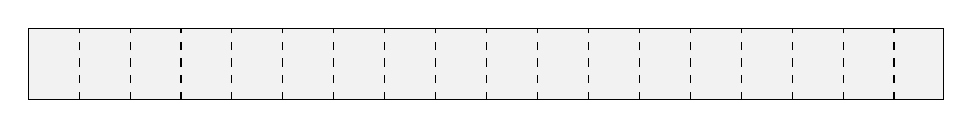
\begin{tikzpicture}[scale=\linewidth/120cm]

    % shaft
    \draw[fill=gray!10] (0,-4.5) -- (115.0, -4.5) -- (115.0, 4.5) -- (0, 4.5) -- cycle;

    % Devisions
    \draw[dashed] (6.4, -4.5) -- (6.4, 4.5);
    \draw[dashed] (12.8, -4.5) -- (12.8, 4.5);
    \draw[dashed] (19.2, -4.5) -- (19.2, 4.5);
    \draw[dashed] (25.6, -4.5) -- (25.6, 4.5);
    \draw[dashed] (32.0, -4.5) -- (32.0, 4.5);
    \draw[dashed] (38.4, -4.5) -- (38.4, 4.5);
    \draw[dashed] (44.8, -4.5) -- (44.8, 4.5);
    \draw[dashed] (51.2, -4.5) -- (51.2, 4.5);
    \draw[dashed] (57.6, -4.5) -- (57.6, 4.5);
    \draw[dashed] (64.0, -4.5) -- (64.0, 4.5);
    \draw[dashed] (70.4, -4.5) -- (70.4, 4.5);
    \draw[dashed] (76.8, -4.5) -- (76.8, 4.5);
    \draw[dashed] (83.2, -4.5) -- (83.2, 4.5);
    \draw[dashed] (89.6, -4.5) -- (89.6, 4.5);
    \draw[dashed] (96.0, -4.5) -- (96.0, 4.5);
    \draw[dashed] (102.4, -4.5) -- (102.4, 4.5);
    \draw[dashed] (108.8, -4.5) -- (108.8, 4.5);
        
\end{tikzpicture}
    \caption{Coarse Model}
    \label{fig:coarse_model}
\end{figure}

The fine model (figure \ref{fig:fine_model}) have more complex geometry. Here the shaft is broken up into 6 section with varying diameter and length, each with one element. This includes more of the intrecasiess of the orginal geometry. The diamters are round giving a slightly different diamter at the ends.
\begin{figure}[ht]
    \centering
    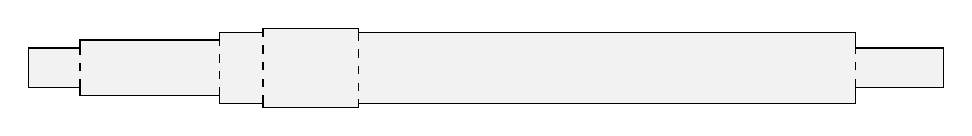
\begin{tikzpicture}[scale=\linewidth/120cm]

    % shaft
    \draw[fill=gray!10] (0,-2.5) -- (6.5,-2.5) -- (6.5,-3.5) -- (24.0, -3.5) -- (24.0, -4.485) -- (29.5, -4.485) -- (29.5, -4.985) -- (41.5, -4.985) -- (41.5, -4.485) -- (104.0, -4.485) -- (104.0, -2.5) -- (115.0, -2.5) -- (115.0, 2.5) -- (104.0, 2.5) -- (104.0, 4.485) -- (41.5, 4.485) -- (41.5, 4.985) -- (29.5, 4.985) -- (29.5, 4.485) -- (24.0, 4.485) -- (24.0, 3.5) -- (6.5, 3.5) -- (6.5, 2.5) -- (0, 2.5) -- cycle;

    % Devisions
    \draw[dashed] (6.5, -2.5) -- (6.5, 2.5);
    \draw[dashed] (24, -3.5) -- (24, 3.5);
    \draw[dashed] (29.5, -4.485) -- (29.5, 4.485);
    \draw[dashed] (41.5, -4.985) -- (41.5, 4.985);
    \draw[dashed] (104, -4.485) -- (104, 4.485);
    
\end{tikzpicture}
    \caption{Fine Model}
    \label{fig:fine_model}
\end{figure}

The very fine model (figure \ref{fig:very_fine_model}) have the same 6 sections as the mechanical geometry (figure \ref{fig:shaft_geometry}) discretizes into approximatly equally sized elements. The very fine mesh consist of 19 elements in total.
\begin{figure}[ht]
    \centering
    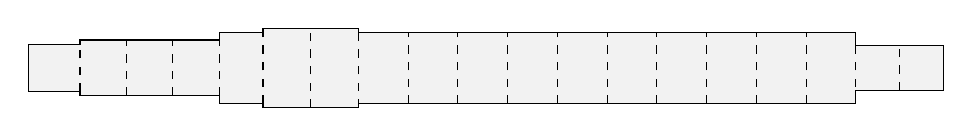
\begin{tikzpicture}[scale=\linewidth/120cm]

    % shaft
    \draw[fill=gray!10] (0,-2.975) -- (6.5,-2.975) -- (6.5,-3.5) -- (24.0, -3.5) -- (24.0, -4.485) -- (29.5, -4.485) -- (29.5, -4.985) -- (41.5, -4.985) -- (41.5, -4.485) -- (104.0, -4.485) -- (104.0, -2.8225) -- (115.0, -2.8225) -- (115.0, 2.8225) -- (104.0, 2.8225) -- (104.0, 4.485) -- (41.5, 4.485) -- (41.5, 4.985) -- (29.5, 4.985) -- (29.5, 4.485) -- (24.0, 4.485) -- (24.0, 3.5) -- (6.5, 3.5) -- (6.5, 2.975) -- (0, 2.975) -- cycle;

    % Devisions
    \draw[dashed] (6.5, -2.975) -- (6.5, 2.975);

    \draw[dashed] (12.3, -3.5) -- (12.3, 3.5);
    \draw[dashed] (18.1, -3.5) -- (18.1, 3.5);
    \draw[dashed] (24, -3.5) -- (24, 3.5);

    \draw[dashed] (29.5, -4.485) -- (29.5, 4.485);

    \draw[dashed] (35.5, -4.985) -- (35.5, 4.985);
    \draw[dashed] (41.5, -4.985) -- (41.5, 4.985);

    \draw[dashed] (47.75, -4.485) -- (47.75, 4.485);
    \draw[dashed] (54, -4.485) -- (54, 4.485);
    \draw[dashed] (60.25, -4.485) -- (60.25, 4.485);
    \draw[dashed] (66.5, -4.485) -- (66.5, 4.485);
    \draw[dashed] (72.75, -4.485) -- (72.75, 4.485);
    \draw[dashed] (79, -4.485) -- (79, 4.485);
    \draw[dashed] (85.25, -4.485) -- (85.25, 4.485);
    \draw[dashed] (91.5, -4.485) -- (91.5, 4.485);
    \draw[dashed] (97.75, -4.485) -- (97.75, 4.485);
    \draw[dashed] (104, -4.485) -- (104, 4.485);

    \draw[dashed] (109.5, -2.8225) -- (109.5, 2.8225);
    

\end{tikzpicture}
    \caption{Very Fine Model}
    \label{fig:very_fine_model}
\end{figure}

For each of the discretized models, the mathematical model is created the same way:

The goverining equation for the system can be written as:
\begin{equation}
    M \ddot{q} - \Omega G \dot{q} + K q = Q
\end{equation}
Where $M$ is the mass matrix, $G$ is the gyroscopic matrix, $\Omega$ is the rotational speed, $K$ is the stiffness matrix, $q$ is the displacement vector and $Q$ is the force vector. The mass matrix for each element can be found by taking the linear motion into account ( $\mathbf{M_t^e}$) and the angular motion ($\mathbf{M_R^e}$):

\begin{equation}
    \mathbf{M^e} = \mathbf{M_t^e} + \mathbf{M_R^e} 
\end{equation}

For each element this matrices can be found:
\begin{equation}
    \mathbf{M_t^e} = \int_{0}^{l} \mu \Psi^T \Psi ds
    \label{eq:mass_matrix_linear}
\end{equation}
\begin{equation}
    \mathbf{M_R^e} = \int_{0}^{l} I_d \Theta^T \Theta ds
    \label{eq:mass_matrix_angular}
\end{equation}
\begin{equation}
    \mathbf{K_B^e} = \int_{0}^{l} E I \Psi''^T \Psi'' ds
\end{equation}
Where:
\begin{equation}
    \Psi(s) =
    \begin{bmatrix}
        \psi_1(s) & 0 & 0 & \psi_2(s) & \psi_3(s) & 0 & 0 & \psi_4(s) \\
        0 & \psi_1(s) & -\psi_2(s) & 0 & 0 & \psi_3(s) & -\psi_4(s) & 0
    \end{bmatrix}
    \label{eq:psi}
\end{equation}
\begin{equation}
    \Theta(s) = 
    \begin{bmatrix}
        0 & -\theta_1(s) & \theta_2(s) & 0 & 0 & -\theta_3(s) & \theta_4(s) & 0 \\
        \theta_1(s) & 0 & 0 & \theta_2(s) & \theta_3(s) & 0 & 0 & \theta_4(s)
    \end{bmatrix}
    \label{eq:theta}
\end{equation}
Equation \ref{eq:psi} and \ref{eq:theta} are the shape functions for the linear and angular motion.

The elements are then assembled into each global matrix describing the enitre system.

\subsubsection{Undamped natural frequencies}
The eigenvalues of the global stiffness and mass matrix is found to find the natural frequencies of the system. The 4 lowest natural frequencies is found for each of the three models.

To make the system solveable a very small bearing stiffnes of \SI{0.01}{\pascal} is added.

\subsubsection{Convergence}
To compare the three mathematical models, a convergence study is done. Here the 4 lowest (non rigid body) natural frequencies are compared.
The resulting natural frequencies are shown in table \ref{tab:natural_freq}.
\begin{table}[ht]
    \centering
    \caption{Undamped Natural Frequencies of Shaft}
    \label{tab:natural_freq}
    \begin{tabular}{@{}cccc@{}}
        \toprule
        Mode    &   Coarse Model (\si{\hertz})    &   Fine Model (\si{\hertz})  &   Very Fine Model (\si{\hertz}) \\ \midrule
        1       &   303.9   &   392.9   &   371.4   \\
        2       &   828.5   &   1066.2  &   916     \\
        3       &   1601.5  &   1786.4  &   1612.2  \\
        4       &   2602.7  &   3660.2  &   2550.7  \\ \bottomrule
    \end{tabular}
\end{table}

\subsection{Validation}
The experimental results from \cite[6]{Problem} is compared to the mathematical model. The experimantal natural frequencies and the discrepancy between the 3 mathematical models and the experimental results is shown in table \ref{tab:validation}.

\begin{table}[ht]
    \centering
    \caption{Validation of Mathematical Model}
    \label{tab:validation}
    \begin{adjustwidth}{-0.5cm}{-0.5cm}        
    \begin{tabular}{@{}ccccc@{}}
        \toprule
        Mode    &   Experimental (\si{\hertz})    &   Coarse Model (\si{\percent})    &   Fine Model (\si{\percent})  &   Very Fine Model (\si{\percent}) \\ \midrule
        1       &   388     &   21.7   &   -1.3   &   4.3   \\
        2       &   930     &   10.9   &   -14.7  &   1.5     \\
        3       &   1689    &   5.2  &   -5.8  &   4.6  \\
        4       &   2624    &   0.8  &   -39.5  &   2.8  \\ \bottomrule
    \end{tabular}
    \end{adjustwidth}
\end{table}


\subsection{Model adjustment}
As the very fine model is within \SI{5}{\percent} of the experimental results, this model is deemed accurate enough for further analysis. This model is choosen for further analysis and is refered to as system (I)

\section{Lateral Dynamics of Flexible Shaft and Discs}
The next step is to add the discs to the shaft. Both a disc with a width of \SI{80}{\milli \meter} and a disc with a width of \SI{100}{\milli \meter} is implemeted.

\subsection{Modelling}
To implement the disc in the system a mechanical and mathematical model is created.

\subsubsection{Mechanical model}
The discs are assumed to be rigid bodies thats mounted to the shaft at a point. And with a assumtion of axisymmetry the discs can be modelled as a point mass at the mounting point. Therefore only the mass and the moment of inertia in two directions is needed. To calculate these the discs are drawn in CAD and the mass and moment of inertia is calculated. The mass and moment of inertia of the discs is shown in table \ref{tab:disc_mass_moment}.
\begin{table}[ht]
    \centering
    \caption{Mass and Moment of Inertia of Discs}
    \label{tab:disc_mass_moment}
    \begin{tabular}{@{}cccc@{}}
        \toprule
        Width    &   Mass                    &   $Id$   &   $Ip$                       \\ \midrule
        \SI{80}{\milli \meter} &  \SI{35.89}{\kilo \gram}   &   \SI{0.221}{\kilo \gram \square \meter} & \SI{0.403}{\kilo \gram \square \meter} \\ 
        \SI{100}{\milli \meter} &   \SI{45.96}{\kilo \gram}   &   \SI{0.297}{\kilo \gram \square \meter} & \SI{0.518}{\kilo \gram \square \meter}\\ \bottomrule
    \end{tabular}
\end{table}

As the CAD model is nearly a perfect reproduction of the disc, only few simplifications are made. Only small details like the chamfers and raoundings are neglected.

\subsubsection{Mathematical model - one disc}
The mass and moment of inertia of the \SI{100}{\milli \meter} disc is added to the mathematical model of the shaft, in the closest node corresponding to the placement seen in figure \ref{fig:shaft_geometry}.
As the disc is assumed to be rigid the extra stifness of the disc is not added. The natural frequencies of the system is calculated, as before, and shown in table \ref{tab:natural_freq_one_disc}.
\begin{table}[ht]
    \centering
    \caption{Undamped Natural Frequencies of Shaft and One Disc}
    \label{tab:natural_freq_one_disc}
    \begin{tabular}{@{}cc@{}}
        \toprule
        Mode    &   Natural Frequency (\si{\hertz})    \\ \midrule
        1       &   288.8   \\
        2       &   596.5   \\
        3       &   1243.5  \\
        4       &   1852.1  \\ 
        5       &   2.283.5 \\ \bottomrule
    \end{tabular}
\end{table}
This model is refered to as system (II)

\subsubsection{Mathematical model - two discs}
The mass and moment of inertia of the \SI{100}{\milli \meter} disc is added to the mathematical system (II) in the node corresponding to the placement seen in figure \ref{fig:shaft_geometry}.
The disc is assumed to be rigid and the extra stifness of the disc is not added. The natural frequencies of the system is calculated and shown in table \ref{tab:natural_freq_two_discs}.
\begin{table}[ht]
    \centering
    \caption{Undamped Natural Frequencies of Shaft and Two Discs}
    \label{tab:natural_freq_two_discs}
    \begin{tabular}{@{}cc@{}}
        \toprule
        Mode    &   Natural Frequency (\si{\hertz})    \\ \midrule
        1       &   242.5   \\
        2       &   502.4   \\
        3       &   929.8  \\
        4       &   1262.9  \\ 
        5       &   2276.9 \\ \bottomrule
    \end{tabular}
\end{table}
This model is refered to as system (III)

\subsection{Validation}
With the natural frequencies of the systems (II) and (III) the experimental results from \cite[6]{Problem} is compared. The experimantal natural frequencies and the discrepancy between the mathematical models and the experimental results is shown in table \ref{tab:validation_two_discs}.
\begin{table}[ht]
    \begin{adjustwidth}{-1cm}{-1cm}
    \centering
    \caption{Validation of Mathematical Model}
    \label{tab:validation_two_discs}
    \begin{tabular}{@{}ccccc@{}}
        \toprule
        Mode    &   Experimental (\si{\hertz})    &   System (II) (\si{\percent})    &   System (III) (\si{\percent})  \\ \midrule
        1       &   241     &   4       &   -0.6    \\
        2       &   498     &   10.8    &   -0.9    \\
        3       &   708     &   7.8     &   -31.3   \\
        4       &   1250    &   7.2     &   -1      \\ 
        5       &   2350    &   4.2     &   3       \\ \bottomrule
    \end{tabular}
    \end{adjustwidth}
\end{table}

A major discrepancy is seen in the third mode of system (III). This is due to an interaction between the two discs. As the discs is assumed as point masses, this model can not account for this.

\subsection{Model adjustment}
As only one natural frequency is significantly off, both models is deemed accurate enough for further analysis.

\section{Modelling of Ball Bearing}
Including the ball bearings in the locations seen on figure \ref{fig:shaft_geometry} the system (I) is considered with the ball bearing stiffness going from \SIrange{e1}{10e9}{\pascal}.
To include the ball bearings in the mathematical system the stiffness matrix is updated with the ball bearing stiffness in the nodes where the bearings are mounted. The ball bearings are assumes to not have any damping.
The 8 first natural frequencies compared with the stifnees can be seen on figure \ref{fig:ball_bearing_stiffness}.
\begin{figure}[ht]
    \centering
    \begin{tikzpicture}

\begin{axis}[%
width=0.9\linewidth,
height=0.6\linewidth,
xmode=log,
ymode=log,
xlabel={Stiffness [\si{\newton \per \square \meter}]},
ylabel={Eigenfrequency [\si{\hertz}]},
grid=major,
legend pos=south east,
]
\addplot []
  table[row sep=crcr]{%
10	0.558817169537322\\
100	1.76716900355551\\
1000	5.58827870662501\\
10000	17.6715970158956\\
100000	55.879562490757\\
1000000	176.613998439708\\
10000000	555.56285341882\\
100000000	1489.30744562933\\
1000000000	1616.49133852598\\
};
\addlegendentry{1}

\addplot [color=red]
  table[row sep=crcr]{%
10	0.905483025557055\\
100	2.86338849220888\\
1000	9.05476056401027\\
10000	28.6314938158507\\
100000	90.4719654351087\\
1000000	283.9222647486\\
10000000	830.038370073486\\
100000000	1663.06489217114\\
1000000000	3259.85266871539\\
};
\addlegendentry{2}

\addplot [color=blue]
  table[row sep=crcr]{%
10	2333.65180752057\\
100	2333.65333036973\\
1000	2333.66855900639\\
10000	2333.82085866914\\
100000	2335.345179351\\
1000000	2350.71877075002\\
10000000	2515.18902486417\\
100000000	3932.52102629454\\
1000000000	7063.0111266213\\
};
\addlegendentry{3}

\addplot [color=green]
  table[row sep=crcr]{%
10	5755.27680532091\\
100	5755.27748269065\\
1000	5755.28425635248\\
10000	5755.35199440482\\
100000	5756.02951901966\\
1000000	5762.81914536959\\
10000000	5832.13233188595\\
100000000	6622.14946572135\\
1000000000	9716.37500170846\\
};
\addlegendentry{4}

\addplot [color=purple]
  table[row sep=crcr]{%
10	10127.4544127093\\
100	10127.4546794837\\
1000	10127.4573471899\\
10000	10127.4840248031\\
100000	10127.7508468415\\
1000000	10130.4236700464\\
10000000	10157.6171130726\\
100000000	10480.3164842834\\
1000000000	14149.0154727874\\
};
\addlegendentry{5}

\addplot [color=orange]
  table[row sep=crcr]{%
10	16019.1003535951\\
100	16019.1004920402\\
1000	16019.1018765057\\
10000	16019.1157211188\\
100000	16019.2541811847\\
1000000	16020.6401605633\\
10000000	16034.6390047921\\
100000000	16189.7635301771\\
1000000000	19796.3836166394\\
};
\addlegendentry{6}

\addplot [color=cyan]
  table[row sep=crcr]{%
10	22964.4386460796\\
100	22964.4387014646\\
1000	22964.439255301\\
10000	22964.4447938927\\
100000	22964.5001807139\\
1000000	22965.0541637429\\
10000000	22970.6055171908\\
100000000	23027.3181513416\\
1000000000	23809.3940691991\\
};
\addlegendentry{7}

\addplot [color=purple]
  table[row sep=crcr]{%
10	30342.7931571478\\
100	30342.7931709179\\
1000	30342.7933084283\\
10000	30342.7946834812\\
100000	30342.8084342607\\
1000000	30342.9459565207\\
10000000	30344.3226354927\\
100000000	30358.2365901199\\
1000000000	30513.8834687328\\
};
\addlegendentry{8}

\end{axis}
\end{tikzpicture}%
    \caption{The 8 lowest natural frequencies compared to ball bearing stiffness}
    \label{fig:ball_bearing_stiffness}
\end{figure}
As expected, the lowest eigenfrequencies, at the lowest stiffness, can be considered rigid body movements with a very low natural frequency. With increasing stiffness the lowest natural frequencies rises to the same level as the other natural frequencies.

The first mode shape of system (I) is found for a bearing stifness of \SI{e1}{\pascal} and \SI{e9}{\pascal} and shown in figure \ref{fig:mode_shape}.
\begin{figure}[ht]
    \begin{subfigure}[t]{0.45\textwidth}
        \centering
        
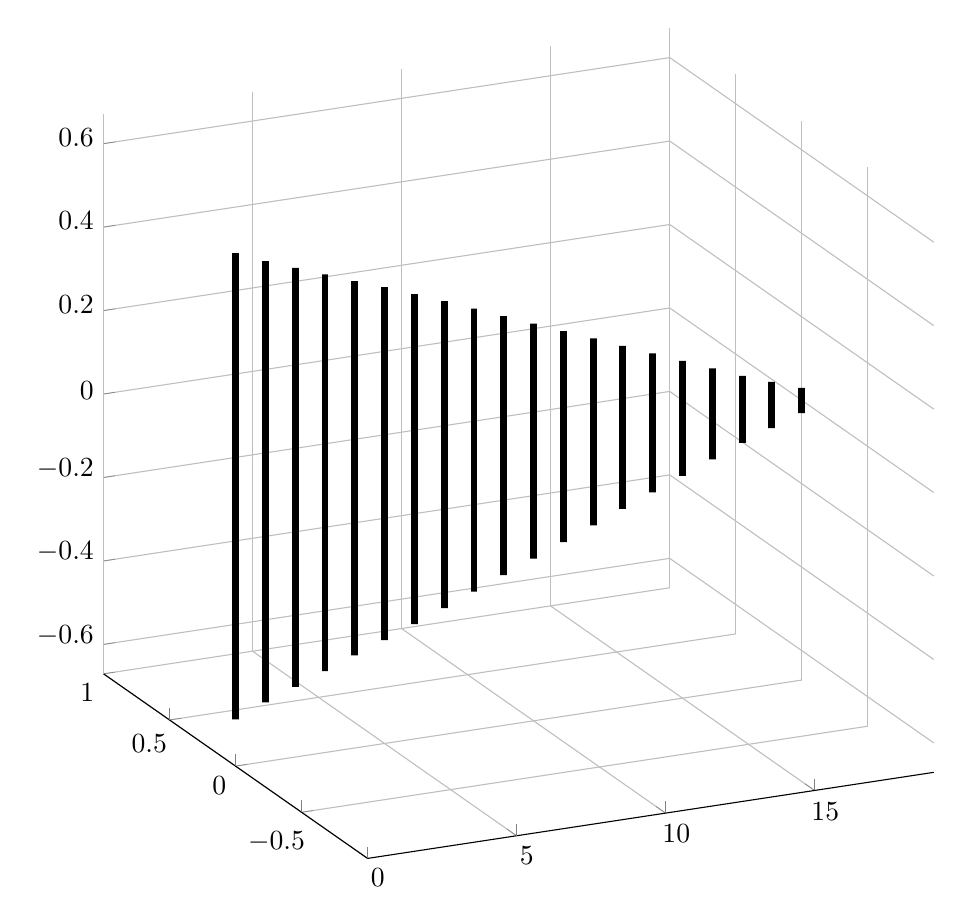
\begin{tikzpicture}

\begin{axis}[%
width=1\linewidth,
height=1\linewidth,
view={-25}{20},
axis x line*=bottom,
axis y line*=left,
axis z line*=left,
xmajorgrids,
ymajorgrids,
zmajorgrids
]
\addplot3 [color=black, line width=2.5pt]
 table[row sep=crcr] {%
0	0	0\\
0	0	-0.0451085412117611\\
0	0	-0.0899226863402309\\
0	0	-0.134149960646758\\
0	0	-0.177501719542518\\
0	0	-0.219695032396641\\
0	0	-0.260454529052796\\
0	0	-0.299514197003149\\
0	0	-0.336619117490623\\
0	0	-0.371527129208979\\
0	0	-0.404010408742755\\
0	0	-0.43385695743249\\
0	0	-0.46087198496136\\
0	0	-0.484879180633413\\
0	0	-0.505721864046515\\
0	0	-0.523264007650291\\
0	0	-0.537391124515418\\
0	0	-0.548011015520367\\
0	0	-0.555054371079127\\
0	0	-0.558475223482836\\
0	0	-0.55825124690312\\
0	0	-0.554383903099241\\
0	0	-0.546898431878073\\
0	0	-0.535843686369199\\
0	0	-0.521291814190169\\
0	0	-0.50333778658277\\
0	0	-0.482098778593345\\
0	0	-0.457713404342347\\
0	0	-0.430340812374072\\
0	0	-0.400159646990652\\
0	0	-0.367366882349072\\
0	0	-0.332176536930345\\
0	0	-0.294818276770715\\
0	0	-0.255535916570773\\
0	0	-0.214585828464811\\
0	0	-0.172235268835434\\
0	0	-0.128760634093281\\
0	0	-0.0844456568053291\\
0	0	-0.0395795539445564\\
0	-0	0.00554486065378761\\
0	-0	0.050633087310446\\
0	-0	0.0953908625229056\\
0	-0	0.139526079444759\\
0	-0	0.182750694289886\\
0	-0	0.224782606219502\\
0	-0	0.265347498443197\\
0	-0	0.304180628518208\\
0	-0	0.341028556162743\\
0	-0	0.375650797306944\\
0	-0	0.407821393586522\\
0	-0	0.437330387035925\\
0	-0	0.463985190356606\\
0	-0	0.487611843817488\\
0	-0	0.508056150584594\\
0	-0	0.525184683070238\\
0	-0	0.538885653733951\\
0	-0	0.549069644651935\\
0	-0	0.555670191093609\\
0	-0	0.558644215296584\\
0	0	0.557972307609087\\
0	0	0.553658853164979\\
0	0	0.54573200326465\\
0	0	0.534243491648559\\
0	0	0.519268296862491\\
0	0	0.500904152918081\\
0	0	0.479270911442204\\
0	0	0.454509759478119\\
0	0	0.426782298043286\\
0	0	0.396269487457565\\
0	0	0.363170466324983\\
0	0	0.327701251876877\\
0	0	0.290093330158471\\
0	0	0.250592145259892\\
0	0	0.209455497451488\\
0	0	0.166951860677867\\
0	0	0.123358630391323\\
0	0	0.0789603131600051\\
0	0	0.0340466698661426\\
0	0	-0.0110891753874474\\
0	0	-0.0561526483205568\\
0	0	-0.100849646983208\\
0	0	-0.144888461180664\\
0	0	-0.187981676288904\\
0	0	-0.229848049035514\\
0	0	-0.270214343003903\\
0	0	-0.308817111881645\\
0	0	-0.345404418814729\\
0	0	-0.379737480646577\\
0	0	-0.411592226310839\\
0	0	-0.44076075920732\\
0	0	-0.467052714016959\\
0	0	-0.490296499100787\\
0	0	-0.510340416374457\\
0	0	-0.527053651349611\\
0	0	-0.540327126880688\\
0	0	-0.550074215045279\\
0	0	-0.556231302512028\\
0	0	-0.55875820570625\\
0	0	-0.557638433063749\\
0	0	-0.552879292661248\\
};
 \addplot3 [color=black, line width=2.5pt]
 table[row sep=crcr] {%
1	0	0\\
1	0	-0.0426946957518551\\
1	0	-0.0851107491253709\\
1	0	-0.126971336271973\\
1	0	-0.168003258534173\\
1	0	-0.207938725447476\\
1	0	-0.246517102446277\\
1	0	-0.283486611867566\\
1	0	-0.318605976150985\\
1	0	-0.351645992511098\\
1	0	-0.382391028804922\\
1	0	-0.410640430832113\\
1	0	-0.436209831883202\\
1	0	-0.458932355989264\\
1	0	-0.478659707020129\\
1	0	-0.49526313652326\\
1	0	-0.508634283986798\\
1	0	-0.518685884042885\\
1	0	-0.52535233599578\\
1	0	-0.528590131957806\\
1	0	-0.528378140798934\\
1	0	-0.524717746056854\\
1	0	-0.51763283690746\\
1	0	-0.507169652254694\\
1	0	-0.49339647895727\\
1	0	-0.476403206161775\\
1	0	-0.456300738650737\\
1	0	-0.433220273034393\\
1	0	-0.407312441510006\\
1	0	-0.378746328776891\\
1	0	-0.34770836852316\\
1	0	-0.314401126686141\\
1	0	-0.279041979427391\\
1	0	-0.241861694450363\\
1	0	-0.203102924919597\\
1	0	-0.163018625810726\\
1	0	-0.121870403026805\\
1	0	-0.0799268060552814\\
1	0	-0.0374615753084115\\
1	-0	0.00524814441434808\\
1	-0	0.0479236126823133\\
1	-0	0.0902863126032686\\
1	-0	0.132059768534257\\
1	-0	0.172971350470377\\
1	-0	0.212754053335435\\
1	-0	0.251148239562098\\
1	-0	0.287903333588782\\
1	-0	0.322779457214336\\
1	-0	0.355548995137535\\
1	-0	0.385998080464068\\
1	-0	0.413927990486015\\
1	-0	0.439156443624404\\
1	-0	0.4615187890705\\
1	-0	0.480869081361743\\
1	-0	0.497081032879246\\
1	-0	0.510048838050472\\
1	-0	0.519687863878015\\
1	-0	0.525935202287837\\
1	-0	0.528750080692098\\
1	0	0.528114128087105\\
1	0	0.52403149494971\\
1	0	0.516528826149662\\
1	0	0.505655087054708\\
1	0	0.491481243963342\\
1	0	0.474099800950828\\
1	0	0.453624196151217\\
1	0	0.430188061415465\\
1	0	0.403944350177408\\
1	0	0.37506433921949\\
1	0	0.34373651085311\\
1	0	0.310165322808919\\
1	0	0.274569873865243\\
1	0	0.23718247392328\\
1	0	0.1982471278613\\
1	0	0.158017943062836\\
1	0	0.11675747101194\\
1	0	0.074734993778931\\
1	0	0.0322247665796785\\
1	0	-0.0104957721218124\\
1	0	-0.053147811285948\\
1	0	-0.0954529869280589\\
1	0	-0.137135198831259\\
1	0	-0.177922412485064\\
1	0	-0.217548434489611\\
1	0	-0.25575464983849\\
1	0	-0.292291709742006\\
1	0	-0.326921158975459\\
1	0	-0.359416992131734\\
1	0	-0.389567128621491\\
1	0	-0.417174796794509\\
1	0	-0.442059818148877\\
1	0	-0.464059783246769\\
1	0	-0.483031111662319\\
1	0	-0.498849989043958\\
1	0	-0.511413175175573\\
1	0	-0.52063867776277\\
1	0	-0.526466287546831\\
1	0	-0.528857971254031\\
1	0	-0.527798119815732\\
1	0	-0.52329365023931\\
};
 \addplot3 [color=black, line width=2.5pt]
 table[row sep=crcr] {%
2	0	0\\
2	0	-0.0405284241983435\\
2	0	-0.0807923439586039\\
2	0	-0.120528981102704\\
2	0	-0.159478998706323\\
2	0	-0.197388193633679\\
2	0	-0.234009155567179\\
2	0	-0.269102881704472\\
2	0	-0.302440336584747\\
2	0	-0.333803946864244\\
2	0	-0.362989021285471\\
2	0	-0.389805086572874\\
2	0	-0.414077130536347\\
2	0	-0.43564674426963\\
2	0	-0.454373155989142\\
2	0	-0.470134149766008\\
2	0	-0.482826863155289\\
2	0	-0.492368458516757\\
2	0	-0.498696663645917\\
2	0	-0.501770178186912\\
2	0	-0.501568943174887\\
2	0	-0.498094271948684\\
2	0	-0.491368841579482\\
2	0	-0.481436544871302\\
2	0	-0.468362203899309\\
2	0	-0.452231146955448\\
2	0	-0.433148651662449\\
2	0	-0.411239257890652\\
2	0	-0.386645954961823\\
2	0	-0.359529248444595\\
2	0	-0.330066112631995\\
2	0	-0.298448835537595\\
2	0	-0.264883763948297\\
2	0	-0.229589956724039\\
2	0	-0.192797755133507\\
2	0	-0.154747279556409\\
2	0	-0.115686862363431\\
2	0	-0.0758714272015025\\
2	0	-0.0355608252618013\\
2	-0	0.00498186061132955\\
2	-0	0.0454920329025068\\
2	-0	0.0857053062927735\\
2	-0	0.125359233142184\\
2	-0	0.164195016326336\\
2	-0	0.201959198248201\\
2	-0	0.238405315002101\\
2	-0	0.273295504894103\\
2	-0	0.306402060820992\\
2	-0	0.337508916376402\\
2	-0	0.366413055985165\\
2	-0	0.392925839862817\\
2	-0	0.416874235153027\\
2	-0	0.438101945208084\\
2	-0	0.456470429642298\\
2	-0	0.471859808501047\\
2	-0	0.484169644644523\\
2	-0	0.493319599240007\\
2	-0	0.499249956084694\\
2	-0	0.501922011337124\\
2	0	0.501318326113672\\
2	0	0.497442840301565\\
2	0	0.490320846845626\\
2	0	0.479998826676568\\
2	0	0.466544145358159\\
2	0	0.450044613433051\\
2	0	0.430607913336642\\
2	0	0.408360896619142\\
2	0	0.383448756062463\\
2	0	0.356034078095015\\
2	0	0.326295781688713\\
2	0	0.294427950663398\\
2	0	0.260638567019481\\
2	0	0.2251481535656\\
2	0	0.188188334700029\\
2	0	0.150000324738748\\
2	0	0.11083335365593\\
2	0	0.0709430405111031\\
2	0	0.0305897251786147\\
2	0	-0.00996323073278906\\
2	0	-0.0504511626814162\\
2	0	-0.0906098304975324\\
2	0	-0.130177142918648\\
2	0	-0.168894868100191\\
2	0	-0.206510318938094\\
2	0	-0.242778002204238\\
2	0	-0.277461220731814\\
2	0	-0.310333618194148\\
2	0	-0.341180656395114\\
2	0	-0.369801015429801\\
2	0	-0.396007907577395\\
2	0	-0.419630296351317\\
2	0	-0.440514012750616\\
2	0	-0.458522761427508\\
2	0	-0.473539010204425\\
2	0	-0.485464757135242\\
2	0	-0.494222170104523\\
2	0	-0.499754094790521\\
2	0	-0.502024427676766\\
2	0	-0.501018351677811\\
2	0	-0.496742432841364\\
};
 \addplot3 [color=black, line width=2.5pt]
 table[row sep=crcr] {%
3	0	0\\
3	0	-0.0383621526816279\\
3	0	-0.0764739388651889\\
3	0	-0.114086626042864\\
3	0	-0.150954739023264\\
3	0	-0.186837661999092\\
3	0	-0.221501208900539\\
3	0	-0.254719151785698\\
3	0	-0.286274697293097\\
3	0	-0.315961901520452\\
3	0	-0.343587014095581\\
3	0	-0.368969742667542\\
3	0	-0.391944429565435\\
3	0	-0.412361132945523\\
3	0	-0.430086605370683\\
3	0	-0.445005163435593\\
3	0	-0.457019442762142\\
3	0	-0.466051033437654\\
3	0	-0.472040991748824\\
3	0	-0.474950224871578\\
3	0	-0.474759746006216\\
3	0	-0.471470798292738\\
3	0	-0.465104846697622\\
3	0	-0.45570343792501\\
3	0	-0.443327929266576\\
3	0	-0.428059088159704\\
3	0	-0.40999656506742\\
3	0	-0.389258243120278\\
3	0	-0.365979468764678\\
3	0	-0.340312168438718\\
3	0	-0.3124238570405\\
3	0	-0.282496544660013\\
3	0	-0.250725548709693\\
3	0	-0.217318219206162\\
3	0	-0.182492585522459\\
3	0	-0.146475933442588\\
3	0	-0.109503321805091\\
3	0	-0.0718160484166078\\
3	0	-0.0336600752474771\\
3	-0	0.00471557681283409\\
3	-0	0.0430604531640027\\
3	-0	0.0811243000600908\\
3	-0	0.118658697863925\\
3	-0	0.155418682331368\\
3	-0	0.191164343344326\\
3	-0	0.225662390658555\\
3	-0	0.25868767644755\\
3	-0	0.290024664705833\\
3	-0	0.319468837921696\\
3	-0	0.346828031838931\\
3	-0	0.371923689596358\\
3	-0	0.394592027060132\\
3	-0	0.414685101743424\\
3	-0	0.432071778337285\\
3	-0	0.446638584551253\\
3	-0	0.458290451678156\\
3	-0	0.466951335049887\\
3	-0	0.472564710334824\\
3	-0	0.475093942437849\\
3	0	0.474522524595389\\
3	0	0.470854186105051\\
3	0	0.464112867986755\\
3	0	0.454342566734223\\
3	0	0.441607047176555\\
3	0	0.425989426323873\\
3	0	0.407591630913018\\
3	0	0.386533732193572\\
3	0	0.362953162295655\\
3	0	0.337003817293786\\
3	0	0.308855052820563\\
3	0	0.278690578785191\\
3	0	0.246707260410355\\
3	0	0.213113833412334\\
3	0	0.178129541709615\\
3	0	0.141982706550846\\
3	0	0.104909236400546\\
3	0	0.0671510873076848\\
3	0	0.0289546838053234\\
3	0	-0.00943068935281138\\
3	0	-0.0477545141226892\\
3	0	-0.0857666741492712\\
3	0	-0.123219087124226\\
3	0	-0.159867323868658\\
3	0	-0.19547220357407\\
3	0	-0.229801354790405\\
3	0	-0.262630731973531\\
3	0	-0.29374607769459\\
3	0	-0.322944320968254\\
3	0	-0.350034902573856\\
3	0	-0.374841018719818\\
3	0	-0.397200774934742\\
3	0	-0.416968242654409\\
3	0	-0.434014411608992\\
3	0	-0.448228031794821\\
3	0	-0.459516339535667\\
3	0	-0.467805662894984\\
3	0	-0.473041902487941\\
3	0	-0.475190884555293\\
3	0	-0.474238583994769\\
3	0	-0.470191215894414\\
};
 \addplot3 [color=black, line width=2.5pt]
 table[row sep=crcr] {%
4	0	0\\
4	0	-0.036195881246346\\
4	0	-0.0721555339341099\\
4	0	-0.107644271225202\\
4	0	-0.142430479660647\\
4	0	-0.176287130761117\\
4	0	-0.208993262704093\\
4	0	-0.240335422407632\\
4	0	-0.27010905860914\\
4	0	-0.298119856847373\\
4	0	-0.324185007635045\\
4	0	-0.348134399545445\\
4	0	-0.369811729426528\\
4	0	-0.38907552249676\\
4	0	-0.405800055665196\\
4	0	-0.41987617804982\\
4	0	-0.431212023339139\\
4	0	-0.439733609347867\\
4	0	-0.445385320853763\\
4	0	-0.448130272564451\\
4	0	-0.447950549845348\\
4	0	-0.444847325637612\\
4	0	-0.438840852803069\\
4	0	-0.429970331946068\\
4	0	-0.418293655574924\\
4	0	-0.403887030272628\\
4	0	-0.386844479342716\\
4	0	-0.367277229176207\\
4	0	-0.345312983344421\\
4	0	-0.321095089155243\\
4	0	-0.294781602112206\\
4	0	-0.266544254382103\\
4	0	-0.236567334003319\\
4	0	-0.2050464821496\\
4	0	-0.1721874162988\\
4	0	-0.1382045876397\\
4	0	-0.103319781479199\\
4	0	-0.0677606697841616\\
4	0	-0.0317593253046052\\
4	-0	0.00444929302434867\\
4	-0	0.0406288735169058\\
4	-0	0.0765432939996157\\
4	-0	0.111958162837551\\
4	-0	0.146642348666317\\
4	-0	0.180369488846248\\
4	-0	0.212919466794036\\
4	-0	0.244079848550131\\
4	-0	0.273647269206328\\
4	-0	0.301428760145146\\
4	-0	0.327243008428931\\
4	-0	0.350921540119406\\
4	-0	0.372309819804862\\
4	-0	0.391268259159041\\
4	-0	0.407673127949458\\
4	-0	0.421417361549566\\
4	-0	0.43241125968463\\
4	-0	0.440583071850994\\
4	-0	0.445879465588097\\
4	-0	0.448265874547086\\
4	0	0.447726724084405\\
4	0	0.444265532908049\\
4	0	0.437904890113085\\
4	0	0.428686307756339\\
4	0	0.416669949932378\\
4	0	0.40193424011897\\
4	0	0.384575349354615\\
4	0	0.364706568588522\\
4	0	0.34245756929931\\
4	0	0.317973557207936\\
4	0	0.291414324608038\\
4	0	0.262953207498578\\
4	0	0.232775954324929\\
4	0	0.201079513711457\\
4	0	0.168070749097328\\
4	0	0.13396508866434\\
4	0	0.0989851193678605\\
4	0	0.0633591342468124\\
4	0	0.0273196424934961\\
4	0	-0.00889814799285283\\
4	0	-0.0450578656653338\\
4	0	-0.0809235179830722\\
4	0	-0.116261031591369\\
4	0	-0.150839779976485\\
4	0	-0.184434088624986\\
4	0	-0.216824707864386\\
4	0	-0.247800243772751\\
4	0	-0.277158537818586\\
4	0	-0.304707986226928\\
4	0	-0.330268790460952\\
4	0	-0.35367413065794\\
4	0	-0.37477125436133\\
4	0	-0.393422473443327\\
4	0	-0.409506062711787\\
4	0	-0.422917054336699\\
4	0	-0.433567922911537\\
4	0	-0.441389156678486\\
4	0	-0.446329711189517\\
4	0	-0.448357342442537\\
4	0	-0.447458817318423\\
4	0	-0.443639999945568\\
};
 \addplot3 [color=black, line width=2.5pt]
 table[row sep=crcr] {%
5	0	0\\
5	0	-0.0341533968343257\\
5	0	-0.0680838951667487\\
5	0	-0.101570051218666\\
5	0	-0.134393321163979\\
5	0	-0.166339487432065\\
5	0	-0.197200056775906\\
5	0	-0.226773620981027\\
5	0	-0.254867171334732\\
5	0	-0.281297358276877\\
5	0	-0.305891688011224\\
5	0	-0.3284896482678\\
5	0	-0.348943755869116\\
5	0	-0.367120519263387\\
5	0	-0.382901309742914\\
5	0	-0.396183135661689\\
5	0	-0.406879314599389\\
5	0	-0.414920039084948\\
5	0	-0.420252832187574\\
5	0	-0.422842890001837\\
5	0	-0.422673308791646\\
5	0	-0.419745195310685\\
5	0	-0.414077659579296\\
5	0	-0.405707690164976\\
5	0	-0.39468991278043\\
5	0	-0.381096233774689\\
5	0	-0.365015370843987\\
5	0	-0.34655227402518\\
5	0	-0.325827440750527\\
5	0	-0.302976129434044\\
5	0	-0.278147476721894\\
5	0	-0.251503524167972\\
5	0	-0.223218160686983\\
5	0	-0.193475987686989\\
5	0	-0.162471114288005\\
5	0	-0.130405890489529\\
5	0	-0.0974895865548552\\
5	0	-0.0639370272310139\\
5	0	-0.0299671897179772\\
5	-0	0.00419822546268624\\
5	-0	0.0383362413726172\\
5	-0	0.0722240598918763\\
5	-0	0.105640515787109\\
5	-0	0.138367520122856\\
5	-0	0.170191483595727\\
5	-0	0.200904710502216\\
5	-0	0.23030675424255\\
5	-0	0.258205725514053\\
5	-0	0.284419544656209\\
5	-0	0.308777129974149\\
5	-0	0.331119514285088\\
5	-0	0.351300882400685\\
5	-0	0.369189522774322\\
5	-0	0.384668687102465\\
5	-0	0.397637352270013\\
5	-0	0.408010879666887\\
5	-0	0.415721567572892\\
5	-0	0.420719093005772\\
5	-0	0.422970840148786\\
5	0	0.422462113214359\\
5	0	0.419196232354572\\
5	0	0.413194511992543\\
5	0	0.404496121716117\\
5	0	0.393157830641731\\
5	0	0.379253636916827\\
5	0	0.362874284778839\\
5	0	0.344126672322598\\
5	0	0.323133153841327\\
5	0	0.300030741294387\\
5	0	0.274970210113341\\
5	0	0.248115115182182\\
5	0	0.21964072341382\\
5	0	0.189732869889275\\
5	0	0.158586745024834\\
5	0	0.126405620682621\\
5	0	0.0933995235384666\\
5	0	0.0597838643652072\\
5	0	0.0257780321772514\\
5	0	-0.00839603758842424\\
5	0	-0.0425153115102353\\
5	0	-0.0763571137858279\\
5	0	-0.109700579501955\\
5	0	-0.142328096085776\\
5	0	-0.174026723530104\\
5	0	-0.204589584123654\\
5	0	-0.23381721261636\\
5	0	-0.261518858008056\\
5	0	-0.287513728464536\\
5	0	-0.311632171236177\\
5	0	-0.333716779878517\\
5	0	-0.353623421548623\\
5	0	-0.371222177672725\\
5	0	-0.386398191845925\\
5	0	-0.399052419430277\\
5	0	-0.409102273959054\\
5	0	-0.416482166128515\\
5	0	-0.421143931859496\\
5	0	-0.423057146635142\\
5	0	-0.422209324063269\\
5	0	-0.418605997367471\\
};
 \addplot3 [color=black, line width=2.5pt]
 table[row sep=crcr] {%
6	0	0\\
6	0	-0.0319252320889507\\
6	0	-0.0636421075555707\\
6	0	-0.0949436295948029\\
6	0	-0.125625512161436\\
6	0	-0.155487513221191\\
6	0	-0.184334741609\\
6	0	-0.211978928965412\\
6	0	-0.23823965844996\\
6	0	-0.262945542212429\\
6	0	-0.285935339937382\\
6	0	-0.30705901116188\\
6	0	-0.326178694498563\\
6	0	-0.343169607373291\\
6	0	-0.357920860405307\\
6	0	-0.370336181114952\\
6	0	-0.380334542235735\\
6	0	-0.387850690530151\\
6	0	-0.392835572657968\\
6	0	-0.39525665531763\\
6	0	-0.395098137571371\\
6	0	-0.392361053968357\\
6	0	-0.387063267792806\\
6	0	-0.379239354481172\\
6	0	-0.368940375969245\\
6	0	-0.356233547441876\\
6	0	-0.341201798660235\\
6	0	-0.323943232729576\\
6	0	-0.304570485839781\\
6	0	-0.283209992157279\\
6	0	-0.260001158665944\\
6	0	-0.235095455342284\\
6	0	-0.208655426602791\\
6	0	-0.180853630475145\\
6	0	-0.151871512416648\\
6	0	-0.121898221129802\\
6	0	-0.091129374103472\\
6	0	-0.0597657809362078\\
6	0	-0.0280121327738184\\
6	-0	0.00392433358556287\\
6	-0	0.0358351882003366\\
6	-0	0.0675121682812242\\
6	-0	0.0987485373961489\\
6	-0	0.129340434713511\\
6	-0	0.159088205478163\\
6	-0	0.187797704036877\\
6	-0	0.21528156090924\\
6	-0	0.241360405634592\\
6	-0	0.265864037414199\\
6	-0	0.288632535908619\\
6	-0	0.309517304940739\\
6	-0	0.32838204229288\\
6	-0	0.345103629268679\\
6	-0	0.359572934214133\\
6	-0	0.371695524753699\\
6	-0	0.381392284093123\\
6	-0	0.388599927366757\\
6	-0	0.393271414659487\\
6	-0	0.395376258007722\\
6	0	0.394900720375836\\
6	0	0.391847905309465\\
6	0	0.386237736680551\\
6	0	0.378106828656315\\
6	0	0.367508246740795\\
6	0	0.354511161448501\\
6	0	0.339200396870426\\
6	0	0.32167587707866\\
6	0	0.302051973982595\\
6	0	0.280456760892854\\
6	0	0.257031176664489\\
6	0	0.231928105874576\\
6	0	0.205311381037326\\
6	0	0.177354713368656\\
6	0	0.148240559078464\\
6	0	0.118158928589635\\
6	0	0.0873061464552808\\
6	0	0.055883570067483\\
6	0	0.0240962755197477\\
6	0	-0.00784828080024533\\
6	0	-0.0397416161526323\\
6	0	-0.0713755820857315\\
6	0	-0.102543722894714\\
6	0	-0.133042623032743\\
6	0	-0.162673234680844\\
6	0	-0.191242176812265\\
6	0	-0.218562997273129\\
6	0	-0.244457389642525\\
6	0	-0.268756356930349\\
6	0	-0.291301314518135\\
6	0	-0.311945125144659\\
6	0	-0.330553059181574\\
6	0	-0.347003673931968\\
6	0	-0.361189606213165\\
6	0	-0.373018273051095\\
6	0	-0.382412475913194\\
6	0	-0.389310904536395\\
6	0	-0.393668537062021\\
6	0	-0.395456933866146\\
6	0	-0.394664423167764\\
6	0	-0.391296177203425\\
};
 \addplot3 [color=black, line width=2.5pt]
 table[row sep=crcr] {%
7	0	0\\
7	0	-0.0296970674189703\\
7	0	-0.0592003200946897\\
7	0	-0.0883172081951582\\
7	0	-0.11685770345557\\
7	0	-0.144635539377515\\
7	0	-0.171469426877418\\
7	0	-0.197184237450405\\
7	0	-0.221612146127814\\
7	0	-0.244593726768953\\
7	0	-0.265978992538805\\
7	0	-0.285628374781109\\
7	0	-0.303413633898312\\
7	0	-0.319218696293623\\
7	0	-0.332940411912965\\
7	0	-0.3444892274428\\
7	0	-0.353789770770279\\
7	0	-0.3607813428913\\
7	0	-0.365418314056082\\
7	0	-0.36767042156686\\
7	0	-0.367522967284159\\
7	0	-0.364976913552628\\
7	0	-0.360048876920403\\
7	0	-0.352771019692978\\
7	0	-0.343190840029349\\
7	0	-0.331370861950343\\
7	0	-0.317388227282264\\
7	0	-0.301334192198995\\
7	0	-0.283313531648308\\
7	0	-0.263443855549342\\
7	0	-0.241854841224013\\
7	0	-0.218687387071798\\
7	0	-0.194092693011359\\
7	0	-0.168231273690403\\
7	0	-0.14127191090395\\
7	0	-0.11339055205795\\
7	0	-0.0847691618672997\\
7	0	-0.0555945347825444\\
7	0	-0.0260570758958129\\
7	-0	0.00365044171770719\\
7	-0	0.0333341351126842\\
7	-0	0.0628002768300088\\
7	-0	0.0918565592383929\\
7	-0	0.120313349609616\\
7	-0	0.147984927736301\\
7	-0	0.17469069801504\\
7	-0	0.200256368084339\\
7	-0	0.224515086325127\\
7	-0	0.247308530800053\\
7	-0	0.268487942524722\\
7	-0	0.287915096327346\\
7	-0	0.305463202960581\\
7	-0	0.321017736578031\\
7	-0	0.334477182174967\\
7	-0	0.345753698115181\\
7	-0	0.354773689420054\\
7	-0	0.361478288078339\\
7	-0	0.365823737241951\\
7	-0	0.367781676800378\\
7	0	0.367339328469908\\
7	0	0.364499579189745\\
7	0	0.359280962280698\\
7	0	0.351717536489448\\
7	0	0.341858663707765\\
7	0	0.329768686817388\\
7	0	0.315526509763068\\
7	0	0.299225082594391\\
7	0	0.280970794837188\\
7	0	0.260882781153647\\
7	0	0.239092143822641\\
7	0	0.215741097114691\\
7	0	0.190982039145695\\
7	0	0.164976557266878\\
7	0	0.137894373482178\\
7	0	0.109912236775692\\
7	0	0.081212769578277\\
7	0	0.0519832759017333\\
7	0	0.0224145189191497\\
7	0	-0.00730052403060091\\
7	0	-0.0369679208888831\\
7	0	-0.0663940505541954\\
7	0	-0.0953868665296405\\
7	0	-0.123757150293903\\
7	0	-0.151319746215752\\
7	0	-0.177894769952513\\
7	0	-0.203308782446056\\
7	0	-0.227395921854304\\
7	0	-0.249998986030856\\
7	0	-0.27097045848803\\
7	0	-0.29017347114749\\
7	0	-0.307482697595159\\
7	0	-0.322785171010693\\
7	0	-0.33598102143339\\
7	0	-0.346984127552832\\
7	0	-0.355722678770437\\
7	0	-0.36213964386367\\
7	0	-0.366193143194233\\
7	0	-0.36785672203106\\
7	0	-0.367119523204297\\
7	0	-0.363986357963463\\
};
 \addplot3 [color=black, line width=2.5pt]
 table[row sep=crcr] {%
8	0	0\\
8	0	-0.0273760626236868\\
8	0	-0.0545734582943788\\
8	0	-0.0814146861098944\\
8	0	-0.107724569659573\\
8	0	-0.133331400294435\\
8	0	-0.15806805776537\\
8	0	-0.181773100915612\\
8	0	-0.204291821309238\\
8	0	-0.225477252919271\\
8	0	-0.245191131285781\\
8	0	-0.26330479588414\\
8	0	-0.279700029814209\\
8	0	-0.294269831330332\\
8	0	-0.306919112176816\\
8	0	-0.317565318171291\\
8	0	-0.326138967985776\\
8	0	-0.332584106609154\\
8	0	-0.336858670531591\\
8	0	-0.338934762267536\\
8	0	-0.338798832425697\\
8	0	-0.336451768137687\\
8	0	-0.331908887268264\\
8	0	-0.325199838444913\\
8	0	-0.316368407559244\\
8	0	-0.305472232003042\\
8	0	-0.292582424503971\\
8	0	-0.277783109015947\\
8	0	-0.261170871693124\\
8	0	-0.242854130530656\\
8	0	-0.222952427786218\\
8	0	-0.20159564980021\\
8	0	-0.17892317930641\\
8	0	-0.155082985765426\\
8	0	-0.130230659657793\\
8	0	-0.104528397039295\\
8	0	-0.0781439409857092\\
8	0	-0.0512494868355066\\
8	0	-0.0240205583753451\\
8	-0	0.00336513769720687\\
8	-0	0.0307288715574772\\
8	-0	0.057892056714831\\
8	-0	0.0846774155383534\\
8	-0	0.110910136240401\\
8	-0	0.136419013767091\\
8	-0	0.161037567149825\\
8	-0	0.184605126025573\\
8	-0	0.206967879234867\\
8	-0	0.227979878653923\\
8	-0	0.247503991709511\\
8	-0	0.265412796360064\\
8	-0	0.281589412702043\\
8	-0	0.295928265774166\\
8	-0	0.308335774581128\\
8	-0	0.31873096283999\\
8	-0	0.327045987463249\\
8	-0	0.333226581329519\\
8	-0	0.337232407452105\\
8	-0	0.339037322234048\\
8	0	0.338629546091523\\
8	0	0.336011740332034\\
8	0	0.331200989785674\\
8	0	0.324228691302808\\
8	0	0.315140348845872\\
8	0	0.303995276512619\\
8	0	0.290866211428986\\
8	0	0.275838839037997\\
8	0	0.259011233882858\\
8	0	0.240493219533912\\
8	0	0.220405651836821\\
8	0	0.198879630159774\\
8	0	0.176055641787449\\
8	0	0.152082645045727\\
8	0	0.127117097141071\\
8	0	0.101321933059247\\
8	0	0.0748655021875236\\
8	0	0.0479204696003476\\
8	0	0.0206626891791503\\
8	0	-0.00672994407925248\\
8	0	-0.0340786550753857\\
8	0	-0.0612049553637342\\
8	0	-0.0879318080385473\\
8	0	-0.114084783146322\\
8	0	-0.13949319608429\\
8	0	-0.163991221555277\\
8	0	-0.187418975808816\\
8	0	-0.209623560105393\\
8	0	-0.230460058593766\\
8	0	-0.249792484088809\\
8	0	-0.267494665577377\\
8	0	-0.28345107165996\\
8	0	-0.297557564554049\\
8	0	-0.309722079738258\\
8	0	-0.319865226801611\\
8	0	-0.327920807576588\\
8	0	-0.333836248174407\\
8	0	-0.337572942102902\\
8	0	-0.339106502227675\\
8	0	-0.338426919932129\\
8	0	-0.335538630437637\\
};
 \addplot3 [color=black, line width=2.5pt]
 table[row sep=crcr] {%
9	0	0\\
9	0	-0.0250550578719939\\
9	0	-0.0499465965809644\\
9	0	-0.074512164154266\\
9	0	-0.0985914360351045\\
9	0	-0.122027261423658\\
9	0	-0.144666688905011\\
9	0	-0.166361964670254\\
9	0	-0.186971496815953\\
9	0	-0.206360779428613\\
9	0	-0.224403270423172\\
9	0	-0.240981217406428\\
9	0	-0.255986426175469\\
9	0	-0.269320966835603\\
9	0	-0.28089781292937\\
9	0	-0.290641409405437\\
9	0	-0.298488165720578\\
9	0	-0.304386870856578\\
9	0	-0.308299027543475\\
9	0	-0.310199103507894\\
9	0	-0.310074698106699\\
9	0	-0.307926623258475\\
9	0	-0.30376889814462\\
9	0	-0.297628657714659\\
9	0	-0.289545975592888\\
9	0	-0.27957360254214\\
9	0	-0.267776622191552\\
9	0	-0.25423202627521\\
9	0	-0.239028212153799\\
9	0	-0.222264405898663\\
9	0	-0.204050014703427\\
9	0	-0.184503912849621\\
9	0	-0.163753665886359\\
9	0	-0.141934698087386\\
9	0	-0.119189408619\\
9	0	-0.0956662421870801\\
9	0	-0.0715187202285462\\
9	0	-0.0469044389700727\\
9	0	-0.0219840408931249\\
9	-0	0.00307983368206481\\
9	-0	0.0281236080511994\\
9	-0	0.052983836691834\\
9	-0	0.0774982719731445\\
9	-0	0.101506923047787\\
9	-0	0.124853100015099\\
9	-0	0.147384436541027\\
9	-0	0.168953884260751\\
9	-0	0.189420672474158\\
9	-0	0.208651226870803\\
9	-0	0.226520041288398\\
9	-0	0.242910496815395\\
9	-0	0.257715622891876\\
9	-0	0.270838795441504\\
9	-0	0.282194367478249\\
9	-0	0.29170822807231\\
9	-0	0.299318286027195\\
9	-0	0.304974875111291\\
9	-0	0.308641078199228\\
9	-0	0.310292968207563\\
9	0	0.309919764252333\\
9	0	0.30752390200935\\
9	0	0.303121017818017\\
9	0	0.296739846632432\\
9	0	0.288422034485772\\
9	0	0.278221866691898\\
9	0	0.266205913558047\\
9	0	0.252452595920818\\
9	0	0.237051673340948\\
9	0	0.220103658297112\\
9	0	0.201719160201949\\
9	0	0.18201816352153\\
9	0	0.161129244709533\\
9	0	0.139188733066736\\
9	0	0.11633982100237\\
9	0	0.0927316295041348\\
9	0	0.0685182349159776\\
9	0	0.0438576633752651\\
9	0	0.0189108594720519\\
9	0	-0.00615936413862005\\
9	0	-0.0311893893161513\\
9	0	-0.0560158602707288\\
9	0	-0.0804767496874668\\
9	0	-0.104412416180396\\
9	0	-0.127666646174942\\
9	0	-0.150087673419162\\
9	0	-0.171529169469999\\
9	0	-0.191851198690262\\
9	0	-0.210921131523634\\
9	0	-0.22861451008733\\
9	0	-0.244815860433191\\
9	0	-0.259419446176097\\
9	0	-0.272329958571201\\
9	0	-0.283463138536292\\
9	0	-0.292746326559707\\
9	0	-0.300118936904882\\
9	0	-0.305532853016707\\
9	0	-0.308952741549084\\
9	0	-0.310356282964244\\
9	0	-0.309734317198832\\
9	0	-0.307090903446084\\
};
 \addplot3 [color=black, line width=2.5pt]
 table[row sep=crcr] {%
10	0	0\\
10	0	-0.0227340531284645\\
10	0	-0.0453197348838239\\
10	0	-0.0676096422229156\\
10	0	-0.0894583024427596\\
10	0	-0.11072312259264\\
10	0	-0.131265320091789\\
10	0	-0.1509508284791\\
10	0	-0.169651172383588\\
10	0	-0.187244306005192\\
10	0	-0.20361540963368\\
10	0	-0.218657639007234\\
10	0	-0.232272822620135\\
10	0	-0.244372102428625\\
10	0	-0.254876513773448\\
10	0	-0.263717500734281\\
10	0	-0.270837363552636\\
10	0	-0.276189635203178\\
10	0	-0.279739384655811\\
10	0	-0.281463444849322\\
10	0	-0.281350563888732\\
10	0	-0.279401478479592\\
10	0	-0.27562890911995\\
10	0	-0.27005747708138\\
10	0	-0.262723543720874\\
10	0	-0.25367497317233\\
10	0	-0.242970819966382\\
10	0	-0.230680943617308\\
10	0	-0.216885552692356\\
10	0	-0.201674681339089\\
10	0	-0.18514760168712\\
10	0	-0.167412175959148\\
10	0	-0.148584152519662\\
10	0	-0.128786410455591\\
10	0	-0.108148157619042\\
10	0	-0.0868040873660354\\
10	0	-0.0648934994946857\\
10	0	-0.0425593911199214\\
10	0	-0.0199475234180676\\
10	-0	0.00279452966792624\\
10	-0	0.025518344554085\\
10	-0	0.0480756166861004\\
10	-0	0.0703191284331864\\
10	-0	0.0921037098882463\\
10	-0	0.113287186303788\\
10	-0	0.133731305980251\\
10	-0	0.153302642550978\\
10	-0	0.171873465775167\\
10	-0	0.189322575155666\\
10	-0	0.20553609094109\\
10	-0	0.220408197349872\\
10	-0	0.233841833165679\\
10	-0	0.245749325197088\\
10	-0	0.256052960467315\\
10	-0	0.264685493399676\\
10	-0	0.271590584688666\\
10	-0	0.276723168992431\\
10	-0	0.280049749046915\\
10	-0	0.281548614282179\\
10	0	0.281209982514123\\
10	0	0.279036063786864\\
10	0	0.275041045949124\\
10	0	0.269251002058741\\
10	0	0.261703720219647\\
10	0	0.252448456961829\\
10	0	0.241545615773844\\
10	0	0.229066352885894\\
10	0	0.215092112876275\\
10	0	0.199714097132027\\
10	0	0.183032668632803\\
10	0	0.165156696942592\\
10	0	0.146202847684118\\
10	0	0.126294821133096\\
10	0	0.105562544901575\\
10	0	0.084141325979237\\
10	0	0.0621709676667565\\
10	0	0.0397948571644724\\
10	0	0.017159029771115\\
10	0	-0.0055887841999945\\
10	0	-0.0283001235670791\\
10	0	-0.0508267651959747\\
10	0	-0.0730216913626075\\
10	0	-0.0947400492484896\\
10	0	-0.115840096307191\\
10	0	-0.136184125331949\\
10	0	-0.155639363187072\\
10	0	-0.174078837337642\\
10	0	-0.191382204522226\\
10	0	-0.207436536160339\\
10	0	-0.222137055368773\\
10	0	-0.235387820776759\\
10	0	-0.247102352677086\\
10	0	-0.257204197426686\\
10	0	-0.265627426413187\\
10	0	-0.272317066330963\\
10	0	-0.277229457958558\\
10	0	-0.28033254109593\\
10	0	-0.281606063801935\\
10	0	-0.281041714566455\\
10	0	-0.278643176554589\\
};
 \addplot3 [color=black, line width=2.5pt]
 table[row sep=crcr] {%
11	0	0\\
11	0	-0.0204130483669287\\
11	0	-0.040692873150788\\
11	0	-0.0607071202380151\\
11	0	-0.0803251687795595\\
11	0	-0.0994189836739238\\
11	0	-0.117863951174598\\
11	0	-0.135539692168387\\
11	0	-0.152330847816851\\
11	0	-0.168127832433465\\
11	0	-0.182827548682914\\
11	0	-0.196334060434852\\
11	0	-0.208559218880831\\
11	0	-0.219423237828093\\
11	0	-0.228855214415651\\
11	0	-0.236793591854249\\
11	0	-0.243186561170178\\
11	0	-0.247992399331023\\
11	0	-0.25117974154658\\
11	0	-0.252727785967817\\
11	0	-0.252626429447922\\
11	0	-0.25087633347941\\
11	0	-0.24748891987697\\
11	0	-0.242486296234202\\
11	0	-0.23590111164077\\
11	0	-0.227776343601597\\
11	0	-0.218165017548768\\
11	0	-0.207129860776696\\
11	0	-0.194742893059129\\
11	0	-0.181084956619779\\
11	0	-0.166245188524168\\
11	0	-0.150320438936076\\
11	0	-0.13341463903528\\
11	0	-0.115638122721792\\
11	0	-0.0971069065334252\\
11	0	-0.0779419324762378\\
11	0	-0.0582682787094266\\
11	0	-0.038214343236061\\
11	0	-0.0179110059272109\\
11	-0	0.00250922565157427\\
11	-0	0.0229130810367588\\
11	-0	0.0431673966422886\\
11	-0	0.0631399848375324\\
11	-0	0.0827004966557552\\
11	-0	0.101721272502748\\
11	-0	0.120078175313554\\
11	-0	0.137651400719783\\
11	-0	0.154326258940045\\
11	-0	0.169993923290577\\
11	-0	0.184552140430988\\
11	-0	0.197905897709775\\
11	-0	0.209968043254269\\
11	-0	0.220659854758026\\
11	-0	0.229911553253575\\
11	-0	0.237662758517398\\
11	-0	0.243862883135024\\
11	-0	0.248471462654394\\
11	-0	0.251458419672789\\
11	-0	0.252804260133796\\
11	0	0.252500200553181\\
11	0	0.250548225343369\\
11	0	0.246961073862385\\
11	0	0.241762157271792\\
11	0	0.234985405746241\\
11	0	0.226675047031809\\
11	0	0.216885317798326\\
11	0	0.205680109669539\\
11	0	0.19313255224124\\
11	0	0.179324535808759\\
11	0	0.164346176918686\\
11	0	0.148295230232842\\
11	0	0.131276450542904\\
11	0	0.113400909099425\\
11	0	0.0947852687171704\\
11	0	0.0755510223876953\\
11	0	0.0558237003682932\\
11	0	0.0357320509221604\\
11	0	0.0154072000565874\\
11	0	-0.00501820425694237\\
11	0	-0.025410857795592\\
11	0	-0.0456376700809635\\
11	0	-0.0655666329799117\\
11	0	-0.0850676822415451\\
11	0	-0.104013546347689\\
11	0	-0.122280577136872\\
11	0	-0.13974955678087\\
11	0	-0.156306475847142\\
11	0	-0.171843277369235\\
11	0	-0.186258562069048\\
11	0	-0.199458250128412\\
11	0	-0.211356195190983\\
11	0	-0.221874746587253\\
11	0	-0.230945256113362\\
11	0	-0.238508526056277\\
11	0	-0.244515195541356\\
11	0	-0.248926062680829\\
11	0	-0.25171234042074\\
11	0	-0.25285584441658\\
11	0	-0.25234911171148\\
11	0	-0.250195449442395\\
};
 \addplot3 [color=black, line width=2.5pt]
 table[row sep=crcr] {%
12	0	0\\
12	0	-0.0180920435696161\\
12	0	-0.0360660113464322\\
12	0	-0.0538045981467169\\
12	0	-0.0711920349755783\\
12	0	-0.0881148445809621\\
12	0	-0.104462582050834\\
12	0	-0.120128555620121\\
12	0	-0.135010522983133\\
12	0	-0.149011358567071\\
12	0	-0.162039687411717\\
12	0	-0.174010481518368\\
12	0	-0.184845614775997\\
12	0	-0.194474372842991\\
12	0	-0.202833914656754\\
12	0	-0.209869682559202\\
12	0	-0.215535758361501\\
12	0	-0.219795163024226\\
12	0	-0.222620097997121\\
12	0	-0.223992126643372\\
12	0	-0.223902294564348\\
12	0	-0.222351188039532\\
12	0	-0.219348930200231\\
12	0	-0.214915114962033\\
12	0	-0.209078679147216\\
12	0	-0.201877713631655\\
12	0	-0.193359214748789\\
12	0	-0.183578777573059\\
12	0	-0.172600233084588\\
12	0	-0.160495231583092\\
12	0	-0.147342775069847\\
12	0	-0.133228701649546\\
12	0	-0.11824512531707\\
12	0	-0.10248983478532\\
12	0	-0.0860656552776151\\
12	0	-0.069079777449836\\
12	0	-0.0516430578220441\\
12	0	-0.0338692952852247\\
12	0	-0.0158744884049627\\
12	-0	0.00222392163082454\\
12	-0	0.0203078174792743\\
12	-0	0.03825917652282\\
12	-0	0.0559608411312166\\
12	-0	0.0732972832783197\\
12	-0	0.0901553585234268\\
12	-0	0.106425044436402\\
12	-0	0.122000158647334\\
12	-0	0.136779051834444\\
12	-0	0.15066527112755\\
12	-0	0.163568189597432\\
12	-0	0.175403597722821\\
12	-0	0.186094252974859\\
12	-0	0.195570383932228\\
12	-0	0.203770145636883\\
12	-0	0.210640023218583\\
12	-0	0.216135181153979\\
12	-0	0.220219755880875\\
12	-0	0.222867089857947\\
12	-0	0.224059905542337\\
12	0	0.223790418149697\\
12	0	0.222060386460753\\
12	0	0.218881101342813\\
12	0	0.21427331206112\\
12	0	0.208267090860989\\
12	0	0.200901636704508\\
12	0	0.192225019442686\\
12	0	0.182293866092701\\
12	0	0.171172991267712\\
12	0	0.158934974171199\\
12	0	0.145659684916529\\
12	0	0.131433763263184\\
12	0	0.116350053171608\\
12	0	0.100506996867002\\
12	0	0.084007992366641\\
12	0	0.0669607186637398\\
12	0	0.0494764329719909\\
12	0	0.0316692446172229\\
12	0	0.0136553703150566\\
12	0	-0.00444762430509512\\
12	0	-0.0225215919795687\\
12	0	-0.0404485748859658\\
12	0	-0.0581115744823011\\
12	0	-0.0753953150855075\\
12	0	-0.0921869962058883\\
12	0	-0.108377028727481\\
12	0	-0.123859750129738\\
12	0	-0.138534114082694\\
12	0	-0.152304349915063\\
12	0	-0.165080587651313\\
12	0	-0.176779444538472\\
12	0	-0.187324569234776\\
12	0	-0.196647140108554\\
12	0	-0.204686314395274\\
12	0	-0.211389625281348\\
12	0	-0.216713324323202\\
12	0	-0.220622666966823\\
12	0	-0.223092139304388\\
12	0	-0.224105624588061\\
12	0	-0.223656508414228\\
12	0	-0.221747721891699\\
};
 \addplot3 [color=black, line width=2.5pt]
 table[row sep=crcr] {%
13	0	0\\
13	0	-0.0157710387262997\\
13	0	-0.031439149450369\\
13	0	-0.0469020759186063\\
13	0	-0.0620589009905726\\
13	0	-0.0768107052639451\\
13	0	-0.0910612126614467\\
13	0	-0.104717418766396\\
13	0	-0.117690197806115\\
13	0	-0.129894884321776\\
13	0	-0.141251825728492\\
13	0	-0.151686902159416\\
13	0	-0.161132010201145\\
13	0	-0.169525507363387\\
13	0	-0.176812614382098\\
13	0	-0.182945772730507\\
13	0	-0.187884955004767\\
13	0	-0.191597926158542\\
13	0	-0.194060453881592\\
13	0	-0.195256466749367\\
13	0	-0.195178159111444\\
13	0	-0.193826042034268\\
13	0	-0.191208939965739\\
13	0	-0.187343933143386\\
13	0	-0.182256246122024\\
13	0	-0.175979083148385\\
13	0	-0.168553411457143\\
13	0	-0.160027693902625\\
13	0	-0.150457572671165\\
13	0	-0.139905506138304\\
13	0	-0.128440361240869\\
13	0	-0.116136964024248\\
13	0	-0.103075611298191\\
13	0	-0.0893415465882412\\
13	0	-0.0750244038029604\\
13	0	-0.0602176222477806\\
13	0	-0.0450178368033455\\
13	0	-0.0295242472482667\\
13	0	-0.0138379708423494\\
13	-0	0.00193861760441989\\
13	-0	0.0177025538701517\\
13	-0	0.0333509563060672\\
13	-0	0.0487816972826056\\
13	-0	0.0638940697145066\\
13	-0	0.078589444314862\\
13	-0	0.0927719132886372\\
13	-0	0.106348916264667\\
13	-0	0.119231844381046\\
13	-0	0.131336618581417\\
13	-0	0.142584238347961\\
13	-0	0.152901297289856\\
13	-0	0.162220462222257\\
13	-0	0.17048091260914\\
13	-0	0.177628737502052\\
13	-0	0.18361728738416\\
13	-0	0.188407478623352\\
13	-0	0.19196804854739\\
13	-0	0.194275759476407\\
13	-0	0.195315550381147\\
13	0	0.195080635177166\\
13	0	0.19357254701349\\
13	0	0.190801128266677\\
13	0	0.186784466305601\\
13	0	0.181548775446164\\
13	0	0.175128225866363\\
13	0	0.167564720598263\\
13	0	0.158907622052332\\
13	0	0.149213429858932\\
13	0	0.138545412129505\\
13	0	0.126973192543994\\
13	0	0.114572295959321\\
13	0	0.101423655504462\\
13	0	0.0876130843790145\\
13	0	0.0732307158024991\\
13	0	0.0583704147695191\\
13	0	0.0431291654498817\\
13	0	0.0276064382317581\\
13	0	0.0119035405388033\\
13	0	-0.00387704434193862\\
13	0	-0.0196323261062784\\
13	0	-0.035259479588117\\
13	0	-0.0506565158369265\\
13	0	-0.0657229477377575\\
13	0	-0.0803604458296781\\
13	0	-0.0944734800425133\\
13	0	-0.10796994316366\\
13	0	-0.120761751965986\\
13	0	-0.132765422073618\\
13	0	-0.143902612813817\\
13	0	-0.154100638499024\\
13	0	-0.163292942802246\\
13	0	-0.171419533129828\\
13	0	-0.178427372156717\\
13	0	-0.184270723968905\\
13	0	-0.188911452553996\\
13	0	-0.192319270691825\\
13	0	-0.194471937620766\\
13	0	-0.195355404189693\\
13	0	-0.19496390454827\\
13	0	-0.19329999377715\\
};
 \addplot3 [color=black, line width=2.5pt]
 table[row sep=crcr] {%
14	0	0\\
14	0	-0.0134500338334397\\
14	0	-0.0268122874555418\\
14	0	-0.0399995535431559\\
14	0	-0.0529257668106129\\
14	0	-0.0655065657056324\\
14	0	-0.0776598429859964\\
14	0	-0.089306281583709\\
14	0	-0.100369872259381\\
14	0	-0.110778409668425\\
14	0	-0.120463963601533\\
14	0	-0.129363322323949\\
14	0	-0.137418405120107\\
14	0	-0.144576641351229\\
14	0	-0.150791313551996\\
14	0	-0.156021862327099\\
14	0	-0.160234151057806\\
14	0	-0.163400688690966\\
14	0	-0.165500809156435\\
14	0	-0.166520806241978\\
14	0	-0.1664540230454\\
14	0	-0.165300895420112\\
14	0	-0.163068949130577\\
14	0	-0.15977275073621\\
14	0	-0.155433812524287\\
14	0	-0.150080452112289\\
14	0	-0.143747607635997\\
14	0	-0.136476609729474\\
14	0	-0.128314911785089\\
14	0	-0.119315780254012\\
14	0	-0.109537947008404\\
14	0	-0.0990452260341128\\
14	0	-0.0879060969555059\\
14	0	-0.0761932581105017\\
14	0	-0.0639831520926215\\
14	0	-0.0513554668565556\\
14	0	-0.0383926156432264\\
14	0	-0.0251791991185603\\
14	0	-0.0118014532362651\\
14	-0	0.0016533135719252\\
14	-0	0.0150972902054178\\
14	-0	0.0284427359845447\\
14	-0	0.0416025532807502\\
14	-0	0.0544908559499746\\
14	-0	0.0670235298594136\\
14	-0	0.0791187818494353\\
14	-0	0.0906976735479123\\
14	-0	0.10168463655309\\
14	-0	0.112007965622698\\
14	-0	0.121600286650571\\
14	-0	0.130398996376563\\
14	-0	0.138346670960049\\
14	-0	0.145391440750497\\
14	-0	0.151487328809211\\
14	-0	0.156594550972916\\
14	-0	0.160679775500857\\
14	-0	0.16371634061085\\
14	-0	0.165684428484562\\
14	-0	0.166571194606386\\
14	0	0.166370851591803\\
14	0	0.165084706958132\\
14	0	0.162721154591153\\
14	0	0.159295619963312\\
14	0	0.154830459461015\\
14	0	0.149354814478063\\
14	0	0.142904421227446\\
14	0	0.135521377512766\\
14	0	0.127253867981408\\
14	0	0.11815584965258\\
14	0	0.108286699772582\\
14	0	0.0977108282955369\\
14	0	0.0864972575187009\\
14	0	0.0747191716157959\\
14	0	0.0624534390083077\\
14	0	0.0497801106919316\\
14	0	0.0367818977922851\\
14	0	0.0235436317595694\\
14	0	0.0101517107251559\\
14	0	-0.00330646436660264\\
14	0	-0.0167430601713144\\
14	0	-0.0300703841795028\\
14	0	-0.0432014570324178\\
14	0	-0.0560505801835431\\
14	0	-0.068533895201021\\
14	0	-0.0805699310607631\\
14	0	-0.0920801358584013\\
14	0	-0.102989389469913\\
14	0	-0.113226493815099\\
14	0	-0.122724637524261\\
14	0	-0.131421831975479\\
14	0	-0.139261315856742\\
14	0	-0.146191925612599\\
14	0	-0.152168429357642\\
14	0	-0.157151822077587\\
14	0	-0.161109580191338\\
14	0	-0.164015873812669\\
14	0	-0.165851735326223\\
14	0	-0.16660518317763\\
14	0	-0.166271300069845\\
14	0	-0.164852265055363\\
};
 \addplot3 [color=black, line width=2.5pt]
 table[row sep=crcr] {%
15	0	0\\
15	0	-0.0111290288933249\\
15	0	-0.0221854253665135\\
15	0	-0.033097031027173\\
15	0	-0.0437926324447064\\
15	0	-0.0542024259171719\\
15	0	-0.0642584730376996\\
15	0	-0.0738951440872572\\
15	0	-0.0830495463600124\\
15	0	-0.0916619346258696\\
15	0	-0.0996761010513424\\
15	0	-0.107039742033984\\
15	0	-0.113704799556269\\
15	0	-0.119627774831123\\
15	0	-0.124770012192112\\
15	0	-0.129097951375531\\
15	0	-0.132583346547885\\
15	0	-0.135203450649306\\
15	0	-0.136941163849815\\
15	0	-0.137785145149542\\
15	0	-0.137729886394545\\
15	0	-0.136775748225196\\
15	0	-0.134928957722496\\
15	0	-0.132201567767696\\
15	0	-0.128611378380455\\
15	0	-0.124181820548907\\
15	0	-0.118941803309816\\
15	0	-0.112925525076833\\
15	0	-0.106172250448198\\
15	0	-0.098726053950522\\
15	0	-0.090635532391093\\
15	0	-0.0819534876959968\\
15	0	-0.072736582303976\\
15	0	-0.0630449693650683\\
15	0	-0.0529419001574872\\
15	0	-0.0424933112849006\\
15	0	-0.0317673943482204\\
15	0	-0.0208341509003904\\
15	0	-0.00976493558871806\\
15	-0	0.00136800953362184\\
15	-0	0.0124920264876417\\
15	-0	0.0235345155630928\\
15	-0	0.0344234091327302\\
15	-0	0.0450876419939969\\
15	-0	0.0554576151684879\\
15	-0	0.0654656501322611\\
15	-0	0.0750464305125047\\
15	-0	0.0841374283678789\\
15	-0	0.0926793122704558\\
15	-0	0.100616334525956\\
15	-0	0.107896695005131\\
15	-0	0.11447287921178\\
15	-0	0.120301968381043\\
15	-0	0.125345919584143\\
15	-0	0.1295718140115\\
15	-0	0.132952071813836\\
15	-0	0.135464632099116\\
15	-0	0.137093096910609\\
15	-0	0.137826838246401\\
15	0	0.13766106742192\\
15	0	0.136596866322773\\
15	0	0.134641180343932\\
15	0	0.13180677306136\\
15	0	0.128112142931892\\
15	0	0.123581402565027\\
15	0	0.118244121354556\\
15	0	0.112135132497065\\
15	0	0.105294305656796\\
15	0	0.097766286760532\\
15	0	0.0896002066207194\\
15	0	0.08084936028846\\
15	0	0.0715708592290439\\
15	0	0.0618252585900624\\
15	0	0.0516761619946954\\
15	0	0.0411898064394489\\
15	0	0.0304346300054608\\
15	0	0.0194808252046636\\
15	0	0.00839988087584187\\
15	0	-0.00273588437964989\\
15	0	-0.0138537941775261\\
15	0	-0.0248812886652408\\
15	0	-0.0357463980761271\\
15	0	-0.0463782124324033\\
15	0	-0.05670734433158\\
15	0	-0.0666663817959422\\
15	0	-0.0761903282296326\\
15	0	-0.085217026612002\\
15	0	-0.0936875651587755\\
15	0	-0.101546661803529\\
15	0	-0.108743024990202\\
15	0	-0.115229688421964\\
15	0	-0.120964317581746\\
15	0	-0.125909486023946\\
15	0	-0.13003291963414\\
15	0	-0.133307707262645\\
15	0	-0.135712476357267\\
15	0	-0.137231532448984\\
15	0	-0.137854961580224\\
15	0	-0.137578695007251\\
15	0	-0.136404535754391\\
};
 \addplot3 [color=black, line width=2.5pt]
 table[row sep=crcr] {%
16	0	0\\
16	0	-0.00880802391321331\\
16	0	-0.0175585631977526\\
16	0	-0.0261945083922419\\
16	0	-0.0346594979214124\\
16	0	-0.0428982859339122\\
16	0	-0.0508571028584628\\
16	0	-0.0584840063252319\\
16	0	-0.06572922016217\\
16	0	-0.0725454592538887\\
16	0	-0.0788882381429231\\
16	0	-0.0847161613593255\\
16	0	-0.0899911935837852\\
16	0	-0.0946789078810833\\
16	0	-0.0987487103838136\\
16	0	-0.102174039959996\\
16	0	-0.10493254156147\\
16	0	-0.107006212121734\\
16	0	-0.108381518051039\\
16	0	-0.109049483561916\\
16	0	-0.109005749248699\\
16	0	-0.108250600538718\\
16	0	-0.106788965829491\\
16	0	-0.10463038432406\\
16	0	-0.101788943774405\\
16	0	-0.0982831885392246\\
16	0	-0.0941359985561663\\
16	0	-0.0893744400183468\\
16	0	-0.0840295887297324\\
16	0	-0.0781363272922177\\
16	0	-0.0717331174480453\\
16	0	-0.0648617490633463\\
16	0	-0.0575670673910365\\
16	0	-0.0498966803930562\\
16	0	-0.0419006480320837\\
16	0	-0.033631155560528\\
16	0	-0.0251421729390448\\
16	0	-0.0164891026073442\\
16	0	-0.00772841790607661\\
16	-0	0.00108270549040196\\
16	-0	0.0098867627249703\\
16	-0	0.0186262950570596\\
16	-0	0.0272442648609952\\
16	-0	0.0356844278759776\\
16	-0	0.0438917002782518\\
16	-0	0.0518125181798085\\
16	-0	0.059395187207386\\
16	-0	0.0665902198802847\\
16	-0	0.0733506585851312\\
16	-0	0.0796323820397344\\
16	-0	0.0853943932459277\\
16	-0	0.0905990870521052\\
16	-0	0.0952124955792334\\
16	-0	0.0992045099085902\\
16	-0	0.102549076584412\\
16	-0	0.105224367648996\\
16	-0	0.107212923100533\\
16	-0	0.108501764843954\\
16	-0	0.109082481391078\\
16	0	0.108951282757294\\
16	0	0.108109025196495\\
16	0	0.10656120561282\\
16	0	0.104317925685706\\
16	0	0.101393825942344\\
16	0	0.0978079902078497\\
16	0	0.0935838210567055\\
16	0	0.0887488870783593\\
16	0	0.0833347429537644\\
16	0	0.0773767235171193\\
16	0	0.070913713146841\\
16	0	0.0639878919908167\\
16	0	0.0566444606821667\\
16	0	0.0489313453421336\\
16	0	0.0408988847953629\\
16	0	0.0325995020389333\\
16	0	0.0240873621092567\\
16	0	0.0154180185797452\\
16	0	0.00664805099633936\\
16	0	-0.00216530438286457\\
16	0	-0.0109645281339483\\
16	0	-0.0196921930615573\\
16	0	-0.0282913389913667\\
16	0	-0.0367058445145837\\
16	0	-0.0448807932583372\\
16	0	-0.0527628322915275\\
16	0	-0.0603005203270417\\
16	0	-0.0674446634478275\\
16	0	-0.0741486361657459\\
16	0	-0.0803686857178471\\
16	0	-0.0860642176141116\\
16	0	-0.0911980605730598\\
16	0	-0.0957367091161559\\
16	0	-0.0996505422377406\\
16	0	-0.102914016723365\\
16	0	-0.105505833854855\\
16	0	-0.107409078414126\\
16	0	-0.108611329078546\\
16	0	-0.109104739487377\\
16	0	-0.10888608945021\\
16	0	-0.107956805963192\\
};
 \addplot3 [color=black, line width=2.5pt]
 table[row sep=crcr] {%
17	0	0\\
17	0	-0.00648701890447506\\
17	0	-0.0129317009719252\\
17	0	-0.019291985672177\\
17	0	-0.025526363285473\\
17	0	-0.0315941458112303\\
17	0	-0.0374557325139373\\
17	0	-0.04307286837313\\
17	0	-0.0484088937507037\\
17	0	-0.0534289836461306\\
17	0	-0.0581003749781122\\
17	0	-0.0623925804093347\\
17	0	-0.0662775873188245\\
17	0	-0.0697300406233315\\
17	0	-0.0727274082545759\\
17	0	-0.0752501282123882\\
17	0	-0.0772817362340176\\
17	0	-0.0788089732463864\\
17	0	-0.0798218719000166\\
17	0	-0.0803138216198734\\
17	0	-0.0802816117485776\\
17	0	-0.0797254525004189\\
17	0	-0.0786489735894148\\
17	0	-0.077059200540369\\
17	0	-0.0749665088375334\\
17	0	-0.0723845562101162\\
17	0	-0.0693301934965692\\
17	0	-0.0658233546693877\\
17	0	-0.0618869267381651\\
17	0	-0.0575466003799656\\
17	0	-0.0528307022718604\\
17	0	-0.0477700102198911\\
17	0	-0.0423975522910004\\
17	0	-0.0367483912588768\\
17	0	-0.0308593957705006\\
17	0	-0.024768999726852\\
17	0	-0.0185169514481557\\
17	0	-0.0121440542607074\\
17	0	-0.00569190019831732\\
17	-0	0.000797401443663221\\
17	-0	0.00728149893016628\\
17	-0	0.0137180744904899\\
17	-0	0.0200651205007147\\
17	-0	0.0262812136419818\\
17	-0	0.032325785245365\\
17	-0	0.0381593860589619\\
17	-0	0.0437439437092292\\
17	-0	0.0490430111762682\\
17	-0	0.0540220046614125\\
17	-0	0.0586484292947022\\
17	-0	0.0628920912091868\\
17	-0	0.0667252945979774\\
17	-0	0.0701230224679769\\
17	-0	0.0730630999106171\\
17	-0	0.0755263388240342\\
17	-0	0.07749666314217\\
17	-0	0.0789612137535017\\
17	-0	0.0799104324246619\\
17	-0	0.0803381241812297\\
17	0	0.0802414977385701\\
17	0	0.0796211837188557\\
17	0	0.0784812305353782\\
17	0	0.0768290779710112\\
17	0	0.0746755086232601\\
17	0	0.07203457753279\\
17	0	0.0689235204547017\\
17	0	0.0653626413712141\\
17	0	0.0613751799798897\\
17	0	0.0569871600222274\\
17	0	0.0522272194424886\\
17	0	0.0471264234852087\\
17	0	0.0417180619511916\\
17	0	0.036037431935175\\
17	0	0.0301216074631065\\
17	0	0.0240091975324672\\
17	0	0.0177400941347671\\
17	0	0.0113552119047174\\
17	0	0.00489622109523027\\
17	0	-0.00159472437904189\\
17	0	-0.00807526205473516\\
17	0	-0.014503097393873\\
17	0	-0.0208362798146576\\
17	0	-0.0270334764774679\\
17	0	-0.0330542420392291\\
17	0	-0.0388592826156303\\
17	0	-0.0444107122284704\\
17	0	-0.0496723000644537\\
17	0	-0.0546097069317287\\
17	0	-0.0591907093709616\\
17	0	-0.063385409958307\\
17	0	-0.067166432427756\\
17	0	-0.0705091003394161\\
17	0	-0.0733915981276649\\
17	0	-0.0757951134781123\\
17	0	-0.0777039601041639\\
17	0	-0.0791056801218976\\
17	0	-0.0799911253551142\\
17	0	-0.0803545170399338\\
17	0	-0.080193483539282\\
17	0	-0.0795090758211263\\
};
 \addplot3 [color=black, line width=2.5pt]
 table[row sep=crcr] {%
18	0	0\\
18	0	-0.00444453446490993\\
18	0	-0.00886006214965421\\
18	0	-0.0132177655837243\\
18	0	-0.0174892046804166\\
18	0	-0.0216465023480251\\
18	0	-0.0256625264267074\\
18	0	-0.0295110667636318\\
18	0	-0.033167006270745\\
18	0	-0.0366064848487678\\
18	0	-0.039807055107589\\
18	0	-0.0427478288667624\\
18	0	-0.0454096134799888\\
18	0	-0.0477750370938753\\
18	0	-0.0498286620234837\\
18	0	-0.0515570855047346\\
18	0	-0.0529490271661178\\
18	0	-0.053995402648834\\
18	0	-0.0546893828948935\\
18	0	-0.0550264387162351\\
18	0	-0.0550043703539885\\
18	0	-0.0546233218349662\\
18	0	-0.053885780031688\\
18	0	-0.0527965584320724\\
18	0	-0.0513627657247215\\
18	0	-0.0495937594048225\\
18	0	-0.0475010847034538\\
18	0	-0.0450983992388654\\
18	0	-0.0424013838814901\\
18	0	-0.0394276404144151\\
18	0	-0.0361965766572219\\
18	0	-0.0327292798029215\\
18	0	-0.0290483787946385\\
18	0	-0.0251778966402271\\
18	0	-0.0211430936286726\\
18	0	-0.016970302471509\\
18	0	-0.0126867564451859\\
18	0	-0.0083204116559944\\
18	0	-0.00389976458752067\\
18	-0	0.000546333878614912\\
18	-0	0.0049888667549594\\
18	-0	0.00939884032450152\\
18	-0	0.0137474733650732\\
18	-0	0.0180063849869267\\
18	-0	0.0221477798575843\\
18	-0	0.026144629605112\\
18	-0	0.0299708492159053\\
18	-0	0.0336014672757494\\
18	-0	0.0370127889430904\\
18	-0	0.0401825505908913\\
18	-0	0.04309006510782\\
18	-0	0.0457163569104748\\
18	-0	0.0480442857855055\\
18	-0	0.0500586587533882\\
18	-0	0.0517463292237852\\
18	-0	0.0530962827953655\\
18	-0	0.0540997091401196\\
18	-0	0.0547500595030262\\
18	-0	0.0550430894418032\\
18	0	0.0549768865278074\\
18	0	0.0545518828272963\\
18	0	0.0537708520815936\\
18	0	0.0526388916045627\\
18	0	0.0511633890155305\\
18	0	0.0493539740247789\\
18	0	0.0472224555862667\\
18	0	0.0447827448277518\\
18	0	0.0420507642612988\\
18	0	0.039044343866703\\
18	0	0.035783104726028\\
18	0	0.0322883309687072\\
18	0	0.0285828308629421\\
18	0	0.0246907879599732\\
18	0	0.0206376032627114\\
18	0	0.0164497294488024\\
18	0	0.0121544982300463\\
18	0	0.00777994197489639\\
18	0	0.00335461075819555\\
18	0	-0.00109261396784188\\
18	0	-0.00553270786534792\\
18	0	-0.00993669313504644\\
18	0	-0.0142758276367697\\
18	0	-0.0185217924719707\\
18	0	-0.0226468768039942\\
18	0	-0.0266241587098967\\
18	0	-0.0304276808835053\\
18	0	-0.0340326200430084\\
18	0	-0.037415448937456\\
18	0	-0.0405540898948551\\
18	0	-0.0434280589097401\\
18	0	-0.0460185993298508\\
18	0	-0.0483088042694221\\
18	0	-0.0502837269501717\\
18	0	-0.0519304782498533\\
18	0	-0.0532383108217394\\
18	0	-0.0541986892360328\\
18	0	-0.0548053456854393\\
18	0	-0.0550543208913429\\
18	0	-0.0549439899436162\\
18	0	-0.0544750729054225\\
};
 \addplot3 [color=black, line width=2.5pt]
 table[row sep=crcr] {%
19	0	0\\
19	0	-0.00240205001397654\\
19	0	-0.00478842330472089\\
19	0	-0.00714354546146308\\
19	0	-0.0094520460306262\\
19	0	-0.0116988588294524\\
19	0	-0.0138693202738377\\
19	0	-0.01594926507865\\
19	0	-0.0179251187059514\\
19	0	-0.0197839859577726\\
19	0	-0.021513735135247\\
19	0	-0.0231030772148493\\
19	0	-0.024541639525004\\
19	0	-0.0258200334422198\\
19	0	-0.0269299156649395\\
19	0	-0.0278640426652079\\
19	0	-0.0286163179627846\\
19	0	-0.0291818319131718\\
19	0	-0.0295568937498856\\
19	0	-0.0297390556718498\\
19	0	-0.0297271288187089\\
19	0	-0.0295211910297976\\
19	0	-0.0291225863361318\\
19	0	-0.0285339161887324\\
19	0	-0.0277590224805336\\
19	0	-0.0268029624726776\\
19	0	-0.0256719757888398\\
19	0	-0.0243734436929901\\
19	0	-0.0229158409163606\\
19	0	-0.0213086803480164\\
19	0	-0.0195624509499995\\
19	0	-0.0176885493022367\\
19	0	-0.0156992052239764\\
19	0	-0.0136074019571773\\
19	0	-0.0114267914327647\\
19	0	-0.00917160517275913\\
19	0	-0.00685656140976585\\
19	0	-0.0044967690299994\\
19	0	-0.00210762896674918\\
19	-0	0.000295266312169187\\
19	-0	0.00269623456699197\\
19	-0	0.00507960613447277\\
19	-0	0.00742982619426833\\
19	-0	0.00973155628581466\\
19	-0	0.0119697744131539\\
19	-0	0.0141298730843891\\
19	-0	0.0161977546459217\\
19	-0	0.0181599232892846\\
19	-0	0.0200035731300967\\
19	-0	0.0217166717843011\\
19	-0	0.0232880388962371\\
19	-0	0.0247074191060385\\
19	-0	0.0259655489801461\\
19	-0	0.0270542174681189\\
19	-0	0.0279663194911791\\
19	-0	0.0286959023127509\\
19	-0	0.0292382043883609\\
19	-0	0.0295896864413505\\
19	-0	0.0297480545615872\\
19	0	0.0297122751764245\\
19	0	0.0294825817962037\\
19	0	0.0290604734902736\\
19	0	0.028448705103474\\
19	0	0.0276512692769349\\
19	0	0.0266733703905298\\
19	0	0.0255213905970458\\
19	0	0.0242028481697439\\
19	0	0.0227263484351502\\
19	0	0.0211015276113106\\
19	0	0.0193389899180411\\
19	0	0.0174502383696183\\
19	0	0.0154475997015832\\
19	0	0.013344143921617\\
19	0	0.0111535990095293\\
19	0	0.00889026132306226\\
19	0	0.00656890229423661\\
19	0	0.00420467202517581\\
19	0	0.00181300041258039\\
19	0	-0.000590503553847169\\
19	0	-0.00299015366180908\\
19	0	-0.00537028885080376\\
19	0	-0.00771537542236705\\
19	0	-0.0100101084190984\\
19	0	-0.012239511510833\\
19	0	-0.0143890347360636\\
19	0	-0.0164446494607121\\
19	0	-0.0183929399345142\\
19	0	-0.0202211908474819\\
19	0	-0.021917470315019\\
19	0	-0.0234707077500926\\
19	0	-0.0248707661142389\\
19	0	-0.0261085080758637\\
19	0	-0.0271758556440624\\
19	0	-0.0280658428887661\\
19	0	-0.0287726614031415\\
19	0	-0.0292916982115383\\
19	0	-0.0296195658755829\\
19	0	-0.0297541246019338\\
19	0	-0.0296944962074143\\
19	0	-0.0294410698503819\\
};
 \end{axis}

\end{tikzpicture}%
        \caption{}
        \label{fig:mode_shape_low_stiffness}
    \end{subfigure}
    \hfill
    \begin{subfigure}[t]{0.45\textwidth}
        \centering
        % This file was created by matlab2tikz.
%
%The latest updates can be retrieved from
%  http://www.mathworks.com/matlabcentral/fileexchange/22022-matlab2tikz-matlab2tikz
%where you can also make suggestions and rate matlab2tikz.
%
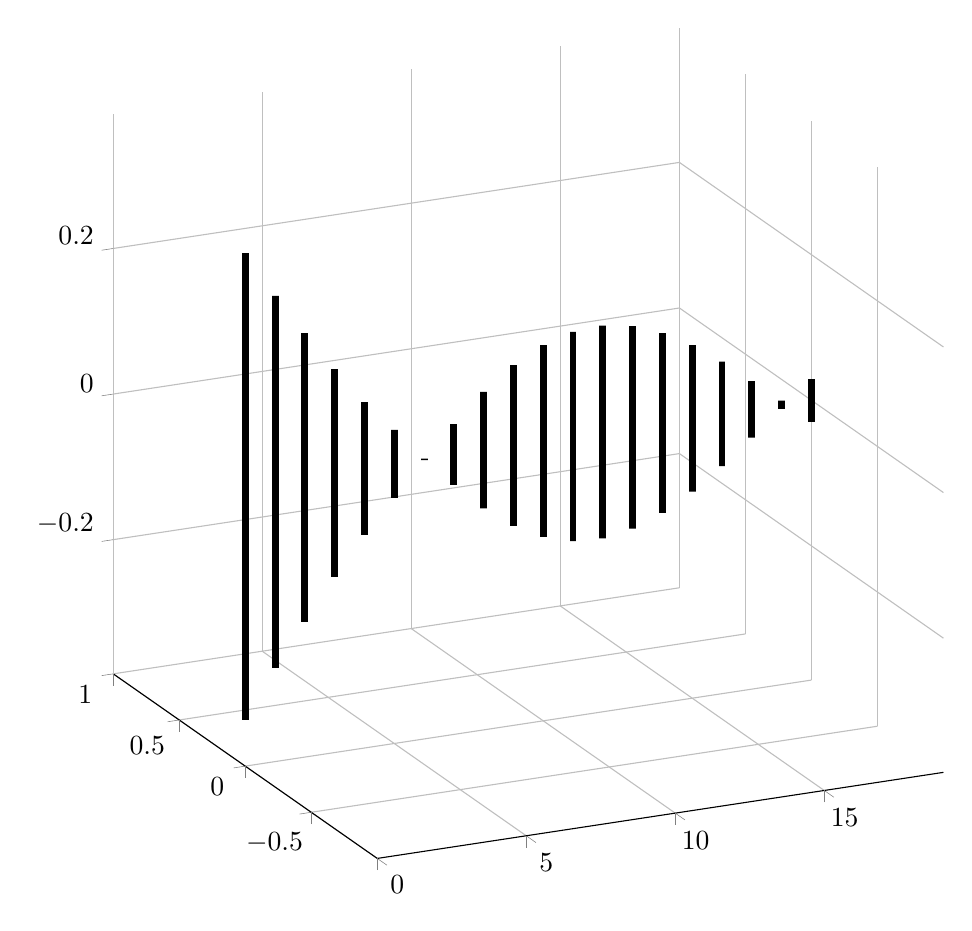
\begin{tikzpicture}

\begin{axis}[%
width=1\linewidth,
height=1\linewidth,
tick align=outside,
view={-25}{20},
axis x line*=bottom,
axis y line*=left,
axis z line*=left,
xmajorgrids,
ymajorgrids,
zmajorgrids
]
\addplot3 [color=black, line width=2.5pt]
 table[row sep=crcr] {%
0	0	-0.320282904058686\\
0	0	-0.319237757951462\\
0	0	-0.316109140664392\\
0	0	-0.310917470784525\\
0	0	-0.30369663119163\\
0	0	-0.294493747925191\\
0	0	-0.283368882621338\\
0	0	-0.270394640526984\\
0	0	-0.255655696649427\\
0	0	-0.239248243133942\\
0	0	-0.221279361476006\\
0	0	-0.201866323665337\\
0	0	-0.181135826822763\\
0	0	-0.159223166324974\\
0	0	-0.136271352813673\\
0	0	-0.112430178851879\\
0	0	-0.0878552413187397\\
0	0	-0.0627069259230924\\
0	0	-0.0371493604632426\\
0	0	-0.0113493436643922\\
0	0	0.0145247434154509\\
0	0	0.0403040363064895\\
0	0	0.0658202892030899\\
0	0	0.0909069730020881\\
0	0	0.115400362137221\\
0	0	0.139140603116573\\
0	0	0.161972757789343\\
0	0	0.183747814533159\\
0	0	0.204323660762541\\
0	0	0.223566010411534\\
0	0	0.241349280337394\\
0	0	0.257557409925574\\
0	0	0.272084618546951\\
0	0	0.284836095923818\\
0	0	0.295728620899047\\
0	0	0.3046911045701\\
0	0	0.311665054243167\\
0	0	0.316604955179495\\
0	0	0.319478567642473\\
0	-0	0.320267137306839\\
0	-0	0.318965517656781\\
0	-0	0.315582203574126\\
0	-0	0.310139275897395\\
0	-0	0.30267225731357\\
0	-0	0.293229880523064\\
0	-0	0.28187377019095\\
0	-0	0.268678040760156\\
0	-0	0.253728812751457\\
0	-0	0.237123650707083\\
0	-0	0.218970926446139\\
0	-0	0.199389111787486\\
0	-0	0.178506005356049\\
0	-0	0.156457898518721\\
0	-0	0.133388685893298\\
0	-0	0.109448926235595\\
0	-0	0.0847948598337892\\
0	-0	0.0595873888228403\\
0	-0	0.0339910270738683\\
0	-0	0.00817282651191804\\
0	0	-0.0176987131306122\\
0	0	-0.043454744009503\\
0	0	-0.0689271721361616\\
0	0	-0.0939497544251113\\
0	0	-0.118359183661758\\
0	0	-0.141996154309509\\
0	0	-0.164706402200368\\
0	0	-0.186341711323574\\
0	0	-0.206760881141588\\
0	0	-0.225830648120345\\
0	0	-0.24342655545949\\
0	0	-0.259433765346417\\
0	0	-0.273747808433005\\
0	0	-0.286275265643674\\
0	0	-0.296934377865019\\
0	0	-0.305655579537947\\
0	0	-0.312381952669874\\
0	0	-0.317069598303939\\
0	0	-0.319687923020857\\
0	0	-0.320219838603615\\
0	0	-0.318661873561892\\
0	0	-0.315024195788372\\
0	0	-0.309330546199077\\
0	0	-0.301618083790811\\
0	0	-0.291937143126931\\
0	0	-0.280350905834185\\
0	0	-0.266934988254565\\
0	0	-0.251776947943319\\
0	0	-0.234975712233898\\
0	0	-0.216640932599269\\
0	0	-0.196892269023274\\
0	0	-0.175858609052501\\
0	0	-0.153677226625462\\
0	0	-0.130492886168874\\
0	0	-0.106456897808064\\
0	0	-0.0817261298575771\\
0	0	-0.0564619850368498\\
0	0	-0.030829347092577\\
0	0	-0.00499550470252365\\
0	0	0.0208709403161884\\
0	0	0.0466011733688597\\
};
 \addplot3 [color=black, line width=2.5pt]
 table[row sep=crcr] {%
1	0	-0.255392830894929\\
1	0	-0.254559433858621\\
1	0	-0.25206468182657\\
1	0	-0.247924856531842\\
1	0	-0.242166976102702\\
1	0	-0.23482861873168\\
1	0	-0.225957677425505\\
1	0	-0.215612047436506\\
1	0	-0.203859248415422\\
1	0	-0.190775983751602\\
1	0	-0.176447639976514\\
1	0	-0.160967729497657\\
1	0	-0.144437280299803\\
1	0	-0.126964176596632\\
1	0	-0.108662454735919\\
1	0	-0.0896515589534662\\
1	0	-0.0700555618330438\\
1	0	-0.0500023545599011\\
1	0	-0.0296228122525868\\
1	0	-0.00904993982044527\\
1	0	0.0115819960787379\\
1	0	0.0321383433157591\\
1	0	0.0524849430827565\\
1	0	0.0724890054663614\\
1	0	0.0920199760869054\\
1	0	0.110950388147655\\
1	0	0.129156694333268\\
1	0	0.146520073128165\\
1	0	0.162927204292487\\
1	0	0.178271008434546\\
1	0	0.192451345853061\\
1	0	0.205375670088234\\
1	0	0.216959631916353\\
1	0	0.227127629846001\\
1	0	0.235813303523132\\
1	0	0.242959966824837\\
1	0	0.248520977815287\\
1	0	0.252460043149345\\
1	0	0.25475145493722\\
1	-0	0.255380258524262\\
1	-0	0.254342350090924\\
1	-0	0.2516445034359\\
1	-0	0.247304325767653\\
1	-0	0.241350142792846\\
1	-0	0.233820813851636\\
1	-0	0.224765478306338\\
1	-0	0.214243234838617\\
1	-0	0.202322755748245\\
1	-0	0.189081838770657\\
1	-0	0.174606899338336\\
1	-0	0.158992406599701\\
1	-0	0.142340266876291\\
1	-0	0.124759158582021\\
1	-0	0.106363822945111\\
1	-0	0.0872743151616895\\
1	-0	0.0676152208683674\\
1	-0	0.047514843047363\\
1	-0	0.0271043646707748\\
1	-0	0.00651699254890428\\
1	0	-0.014112912029785\\
1	0	-0.0346507101932857\\
1	0	-0.0549623641922858\\
1	0	-0.0749153121832445\\
1	0	-0.0943793333791258\\
1	0	-0.113227397921476\\
1	0	-0.131336495927248\\
1	0	-0.148588440299683\\
1	0	-0.164870638063793\\
1	0	-0.180076825192404\\
1	0	-0.194107760126995\\
1	0	-0.206871871467145\\
1	0	-0.218285855601515\\
1	0	-0.228275220379978\\
1	0	-0.236774771278696\\
1	0	-0.243729036885225\\
1	0	-0.249092630926772\\
1	0	-0.252830548478864\\
1	0	-0.254918394421255\\
1	0	-0.255342542650075\\
1	0	-0.254100225007144\\
1	0	-0.251199549346065\\
1	0	-0.246659446617174\\
1	0	-0.240509547316721\\
1	0	-0.232789988106588\\
1	0	-0.223551149866653\\
1	0	-0.212853328889346\\
1	0	-0.200766343362328\\
1	0	-0.187369077707537\\
1	0	-0.172748967750421\\
1	0	-0.157001430079347\\
1	0	-0.140229239319416\\
1	0	-0.122541857384829\\
1	0	-0.104054719087385\\
1	0	-0.0848884787634867\\
1	0	-0.0651682228364857\\
1	0	-0.0450226534534794\\
1	0	-0.0245832485244761\\
1	0	-0.00398340364583643\\
1	0	0.0166424384918584\\
1	0	0.0371596655296898\\
};
 \addplot3 [color=black, line width=2.5pt]
 table[row sep=crcr] {%
2	0	-0.197901113059282\\
2	0	-0.19725532280539\\
2	0	-0.195322166724933\\
2	0	-0.192114261354893\\
2	0	-0.187652542747537\\
2	0	-0.181966129833505\\
2	0	-0.175092134380212\\
2	0	-0.167075418785855\\
2	0	-0.157968303289761\\
2	0	-0.147830224509921\\
2	0	-0.136727347536242\\
2	0	-0.124732134111147\\
2	0	-0.111922869715737\\
2	0	-0.0983831526479535\\
2	0	-0.0842013484271972\\
2	0	-0.0694700130861937\\
2	0	-0.0542852891139161\\
2	0	-0.0387462779918846\\
2	0	-0.0229543934189166\\
2	0	-0.00701269944543771\\
2	0	0.00897476216305168\\
2	0	0.0249036509434625\\
2	0	0.0406700087020211\\
2	0	0.0561709379863338\\
2	0	0.0713052736346353\\
2	0	0.085974243019428\\
2	0	0.100082110676501\\
2	0	0.113536803112225\\
2	0	0.126250509711392\\
2	0	0.138140255823829\\
2	0	0.1491284442896\\
2	0	0.159143361868598\\
2	0	0.168119647269358\\
2	0	0.175998717722552\\
2	0	0.182729151315189\\
2	0	0.188267022590242\\
2	0	0.19257618922146\\
2	0	0.195628527892408\\
2	0	0.197404117840288\\
2	-0	0.197891370866676\\
2	-0	0.197087106966661\\
2	-0	0.194996575082812\\
2	-0	0.191633418848507\\
2	-0	0.187019587544222\\
2	-0	0.181185192847888\\
2	-0	0.174168312314241\\
2	-0	0.166014740865717\\
2	-0	0.156777691916777\\
2	-0	0.146517450082236\\
2	-0	0.135300977736148\\
2	-0	0.123201477989019\\
2	-0	0.110297916935508\\
2	-0	0.0966745082906384\\
2	-0	0.0824201637779635\\
2	-0	0.0676279128566871\\
2	-0	0.0523942955748206\\
2	-0	0.0368187325108542\\
2	-0	0.0210028759159563\\
2	-0	0.0050499462913969\\
2	0	-0.0109359412690454\\
2	0	-0.0268504565751379\\
2	0	-0.0425897352400542\\
2	0	-0.0580510565402172\\
2	0	-0.0731335138111462\\
2	0	-0.0877386730040401\\
2	0	-0.1017712151051\\
2	0	-0.115139558224905\\
2	0	-0.127756455297847\\
2	0	-0.139539563490802\\
2	0	-0.150411981604841\\
2	0	-0.160302751962712\\
2	0	-0.169147323506547\\
2	0	-0.176887973083458\\
2	0	-0.18347418216954\\
2	0	-0.188862966573626\\
2	0	-0.193019156969029\\
2	0	-0.195915628422401\\
2	0	-0.197533477421715\\
2	0	-0.197862145248026\\
2	0	-0.196899486885817\\
2	0	-0.194651785022221\\
2	0	-0.191133709043728\\
2	0	-0.186368219297999\\
2	0	-0.180386417245612\\
2	0	-0.173227342479688\\
2	0	-0.164937717938156\\
2	0	-0.155571644971478\\
2	0	-0.145190250255959\\
2	0	-0.133861286857011\\
2	0	-0.121658692045998\\
2	0	-0.108662104756519\\
2	0	-0.0949563458294043\\
2	0	-0.0806308644385416\\
2	0	-0.0657791543103835\\
2	0	-0.0504981435471136\\
2	0	-0.0348875620357236\\
2	0	-0.0190492905715442\\
2	0	-0.00308669594409935\\
2	0	0.0128960436752213\\
2	0	0.0287946186408878\\
};
 \addplot3 [color=black, line width=2.5pt]
 table[row sep=crcr] {%
3	0	-0.142368348240829\\
3	0	-0.141903772320384\\
3	0	-0.140513076564246\\
3	0	-0.138205337199947\\
3	0	-0.134995615442322\\
3	0	-0.130904859198099\\
3	0	-0.125959766351616\\
3	0	-0.120192610523932\\
3	0	-0.113641030442475\\
3	0	-0.106347784295906\\
3	0	-0.0983604706773605\\
3	0	-0.089731217937304\\
3	0	-0.0805163439734157\\
3	0	-0.0707759886778339\\
3	0	-0.0605737214405643\\
3	0	-0.0499761262706364\\
3	0	-0.0390523672426692\\
3	0	-0.0278737371049155\\
3	0	-0.0165131919947432\\
3	0	-0.00504487529818628\\
3	0	0.00645636623895697\\
3	0	0.0179154709904277\\
3	0	0.0292576523312046\\
3	0	0.0404088867244362\\
3	0	0.0512963968281593\\
3	0	0.0618491264688594\\
3	0	0.0719982043820088\\
3	0	0.0816773936930291\\
3	0	0.0908235242051895\\
3	0	0.0993769046731575\\
3	0	0.107281712371546\\
3	0	0.114486357415978\\
3	0	0.120943819458961\\
3	0	0.126611954563176\\
3	0	0.131453770249383\\
3	0	0.135437666923897\\
3	0	0.138537644109964\\
3	0	0.140733470137099\\
3	0	0.142010814180924\\
3	-0	0.14236133979177\\
3	-0	0.141782759301621\\
3	-0	0.14027884875434\\
3	-0	0.137859423261719\\
3	-0	0.134540272946197\\
3	-0	0.130343059888314\\
3	-0	0.12529517675145\\
3	-0	0.119429568006529\\
3	-0	0.112784514923446\\
3	-0	0.105403385732437\\
3	-0	0.0973343525859524\\
3	-0	0.0886300771682433\\
3	-0	0.0793473670044925\\
3	-0	0.0695468047125618\\
3	-0	0.0592923526169976\\
3	-0	0.048650935305741\\
3	-0	0.0376920028539431\\
3	-0	0.0264870775654557\\
3	-0	0.0151092871901437\\
3	-0	0.00363288766342467\\
3	0	-0.00786722151717419\\
3	0	-0.0193159861155981\\
3	0	-0.0306386869907317\\
3	0	-0.041761427742905\\
3	0	-0.0526116169908645\\
3	0	-0.0631184421316802\\
3	0	-0.0732133314916471\\
3	0	-0.0828304018520001\\
3	0	-0.0919068884287144\\
3	0	-0.100383554500175\\
3	0	-0.108205078009321\\
3	0	-0.115320412617155\\
3	0	-0.121683120851223\\
3	0	-0.127251677174834\\
3	0	-0.131989738999041\\
3	0	-0.135866383868673\\
3	0	-0.138856311274441\\
3	0	-0.140940007774014\\
3	0	-0.142103874344418\\
3	0	-0.14234031513461\\
3	0	-0.141647787038991\\
3	0	-0.140030809768317\\
3	0	-0.13749993635229\\
3	0	-0.134071684266337\\
3	0	-0.129768427632066\\
3	0	-0.124618251194949\\
3	0	-0.118654767032224\\
3	0	-0.111916895187261\\
3	0	-0.104448609662046\\
3	0	-0.0962986514255513\\
3	0	-0.0875202103109949\\
3	0	-0.0781705778780709\\
3	0	-0.0683107735056933\\
3	0	-0.0580051461555281\\
3	0	-0.0473209544053581\\
3	0	-0.0363279274931477\\
3	0	-0.0250978102366082\\
3	0	-0.0137038947982973\\
3	0	-0.00222054235213651\\
3	0	0.00927730222685945\\
3	0	0.0207145994823171\\
};
 \addplot3 [color=black, line width=2.5pt]
 table[row sep=crcr] {%
4	0	-0.0909067307234081\\
4	0	-0.0906100841820784\\
4	0	-0.0897220805901035\\
4	0	-0.0882485154082186\\
4	0	-0.0861990057024244\\
4	0	-0.083586927379231\\
4	0	-0.0804293278892305\\
4	0	-0.0767468149687295\\
4	0	-0.0725634221455552\\
4	0	-0.0679064518868\\
4	0	-0.0628062974121812\\
4	0	-0.0572962443359345\\
4	0	-0.0514122534318024\\
4	0	-0.0451927259388801\\
4	0	-0.0386782529400234\\
4	0	-0.0319113504484761\\
4	0	-0.0249361819316441\\
4	0	-0.017798270082935\\
4	0	-0.0105441997227552\\
4	0	-0.00322131376764734\\
4	0	0.00412259574820468\\
4	0	0.0114395995825902\\
4	0	0.0186819440903589\\
4	0	0.0258023628824931\\
4	0	0.0327543853051548\\
4	0	0.0394926397254511\\
4	0	0.045973149644558\\
4	0	0.0521536207056493\\
4	0	0.0579937167235061\\
4	0	0.063455322934327\\
4	0	0.0685027947476698\\
4	0	0.0731031903770688\\
4	0	0.0772264858310914\\
4	0	0.0808457708617156\\
4	0	0.0839374245911938\\
4	0	0.0864812696711925\\
4	0	0.0884607039681038\\
4	0	0.0898628089151\\
4	0	0.0906784338237823\\
4	-0	0.0909022556051723\\
4	-0	0.090532813510285\\
4	-0	0.0895725186635506\\
4	-0	0.088027638326869\\
4	-0	0.0859082549969923\\
4	-0	0.0832282006031862\\
4	-0	0.0800049662346179\\
4	-0	0.0762595879866288\\
4	-0	0.0720165096709013\\
4	-0	0.0673034232855291\\
4	-0	0.0621510882861453\\
4	-0	0.056593130837615\\
4	-0	0.0506658243564577\\
4	-0	0.0444078527762618\\
4	-0	0.037860058081119\\
4	-0	0.0310651737547699\\
4	-0	0.024067545885081\\
4	-0	0.0169128437440308\\
4	-0	0.00964776173207806\\
4	-0	0.00231971463213637\\
4	0	-0.00502347183794925\\
4	0	-0.0123338731548491\\
4	0	-0.0195637787640389\\
4	0	-0.0266660034576463\\
4	0	-0.0335941953236765\\
4	0	-0.0403031382568231\\
4	0	-0.0467490470565568\\
4	0	-0.0528898531865668\\
4	0	-0.0586854793305763\\
4	0	-0.0640981009526729\\
4	0	-0.0690923931551084\\
4	0	-0.073635761222476\\
4	0	-0.0776985533476445\\
4	0	-0.0812542541511147\\
4	0	-0.0842796577308165\\
4	0	-0.0867550191129529\\
4	0	-0.0886641831154663\\
4	0	-0.0899946897831109\\
4	0	-0.0907378557060219\\
4	0	-0.0908888306910636\\
4	0	-0.090446629416098\\
4	0	-0.0894141378605845\\
4	0	-0.0877980944705425\\
4	0	-0.0856090461808025\\
4	0	-0.0828612795815607\\
4	0	-0.0795727276784713\\
4	0	-0.0757648528547985\\
4	0	-0.0714625067994607\\
4	0	-0.066693768315133\\
4	0	-0.0614897600649368\\
4	0	-0.0558844454536978\\
4	0	-0.049914406969407\\
4	0	-0.0436186074315139\\
4	0	-0.0370381357042414\\
4	0	-0.0302159385344956\\
4	0	-0.0231965402645023\\
4	0	-0.0160257522484357\\
4	0	-0.00875037386950213\\
4	0	-0.00141788710875628\\
4	0	0.00592385334098385\\
4	0	0.0132269323936864\\
};
 \addplot3 [color=black, line width=2.5pt]
 table[row sep=crcr] {%
5	0	-0.0463704644144806\\
5	0	-0.0462191484692372\\
5	0	-0.0457661881808852\\
5	0	-0.0450145397464375\\
5	0	-0.0439691087192365\\
5	0	-0.0426367179933835\\
5	0	-0.0410260632748485\\
5	0	-0.039147656329872\\
5	0	-0.0370137563810441\\
5	0	-0.0346382900987956\\
5	0	-0.0320367607104687\\
5	0	-0.0292261468201574\\
5	0	-0.0262247915996586\\
5	0	-0.0230522830737175\\
5	0	-0.0197293262808736\\
5	0	-0.0162776081442345\\
5	0	-0.0127196559340856\\
5	0	-0.00907869024606271\\
5	0	-0.00537847345441162\\
5	0	-0.00164315462938658\\
5	0	0.002102888069081\\
5	0	0.00583520649284348\\
5	0	0.00952944206376829\\
5	0	0.0131614847474003\\
5	0	0.0167076304045304\\
5	0	0.0201447354937315\\
5	0	0.0234503681152142\\
5	0	0.0266029544102273\\
5	0	0.0295819193605469\\
5	0	0.032367821069138\\
5	0	0.0349424776456223\\
5	0	0.0372890858684461\\
5	0	0.0393923308493143\\
5	0	0.041238485984175\\
5	0	0.0428155025384372\\
5	0	0.0441130882817517\\
5	0	0.0451227746591554\\
5	0	0.0458379720601913\\
5	0	0.0462540128252991\\
5	-0	0.046368181708797\\
5	-0	0.0461797335996431\\
5	-0	0.0456898983843235\\
5	-0	0.0449018729201289\\
5	-0	0.0438208001712067\\
5	-0	0.0424537356435538\\
5	-0	0.0408096013380096\\
5	-0	0.0388991275217685\\
5	-0	0.0367347826984359\\
5	-0	0.0343306922336691\\
5	-0	0.0317025461674847\\
5	-0	0.0288674968148859\\
5	-0	0.0258440468231082\\
5	-0	0.0226519284160651\\
5	-0	0.0193119746140936\\
5	-0	0.0158459832694686\\
5	-0	0.0122765748050453\\
5	-0	0.00862704458448101\\
5	-0	0.00492121087752986\\
5	-0	0.0011832594126447\\
5	0	-0.00256241446859985\\
5	0	-0.00629136502510234\\
5	0	-0.00997925565875667\\
5	0	-0.0136020177446642\\
5	0	-0.0171360077124469\\
5	0	-0.020558161353488\\
5	0	-0.0238461443470297\\
5	0	-0.0269784980227353\\
5	0	-0.029934779408413\\
5	0	-0.0326956946488932\\
5	0	-0.0352432249253166\\
5	0	-0.037560744053034\\
5	0	-0.0396331269906271\\
5	0	-0.0414468485518778\\
5	0	-0.0429900716764542\\
5	0	-0.0442527246832219\\
5	0	-0.0452265670019971\\
5	0	-0.0459052429547487\\
5	0	-0.0462843232352534\\
5	0	-0.0463613338164903\\
5	0	-0.0461357720971142\\
5	0	-0.0456091101816301\\
5	0	-0.0447847852728596\\
5	0	-0.0436681772394037\\
5	0	-0.0422665735045041\\
5	0	-0.0405891214854523\\
5	0	-0.0386467688939467\\
5	0	-0.0364521922870195\\
5	0	-0.0340197143348392\\
5	0	-0.0313652103453315\\
5	0	-0.0285060046556751\\
5	0	-0.025460757566863\\
5	0	-0.0222493435592377\\
5	0	-0.0188927215838155\\
5	0	-0.0154127982759277\\
5	0	-0.0118322849839016\\
5	0	-0.00817454954586789\\
5	0	-0.0044634637820571\\
5	0	-0.000723247697911154\\
5	0	0.00302168858519914\\
5	0	0.00674690414002804\\
};
 \addplot3 [color=black, line width=2.5pt]
 table[row sep=crcr] {%
6	0	-0.000732829710254917\\
6	0	-0.000730438342781895\\
6	0	-0.000723279847367597\\
6	0	-0.000711400943168875\\
6	0	-0.00069487915658707\\
6	0	-0.000673822315300222\\
6	0	-0.00064836784453723\\
6	0	-0.000618681870186754\\
6	0	-0.000584958134594315\\
6	0	-0.000547416732123545\\
6	0	-0.000506302672733795\\
6	0	-0.000461884282948765\\
6	0	-0.000414451454652066\\
6	0	-0.000364313753138759\\
6	0	-0.000311798396770473\\
6	0	-0.000257248121419663\\
6	0	-0.000201018943640497\\
6	0	-0.000143477837164784\\
6	0	-8.5000337887049e-05\\
6	0	-2.59680929695706e-05\\
6	0	3.32336299371181e-05\\
6	0	9.22184571024636e-05\\
6	0	0.000150601430342835\\
6	0	0.000208001519410056\\
6	0	0.000264044108744675\\
6	0	0.00031836344236447\\
6	0	0.00037060501093185\\
6	0	0.000420427865421239\\
6	0	0.000467506842286533\\
6	0	0.000511534685606299\\
6	0	0.000552224052356779\\
6	0	0.000589309387725488\\
6	0	0.000622548658226376\\
6	0	0.000651724931305563\\
6	0	0.000676647791128512\\
6	0	0.000697154581308667\\
6	0	0.000713111466467014\\
6	0	0.000724414305694403\\
6	0	0.000730989332216091\\
6	-0	0.000732793634822725\\
6	-0	0.000729815437925775\\
6	-0	0.000722074178409659\\
6	-0	0.000709620378778985\\
6	-0	0.000692535317428817\\
6	-0	0.000670930498189898\\
6	-0	0.000644946922610787\\
6	-0	0.000614754169726294\\
6	-0	0.000580549289317996\\
6	-0	0.00054255551588985\\
6	-0	0.000501020811752013\\
6	-0	0.000456216248721272\\
6	-0	0.000408434238999739\\
6	-0	0.000357986626777803\\
6	-0	0.000305202653016281\\
6	-0	0.000250426806690395\\
6	-0	0.000194016576519226\\
6	-0	0.000136340117853708\\
6	-0	7.77738499499983e-05\\
6	-0	1.86999993093455e-05\\
6	0	-4.04958948824034e-05\\
6	0	-9.94274969351805e-05\\
6	0	-0.000157710196033375\\
6	0	-0.000214963616357305\\
6	0	-0.000270814099565432\\
6	0	-0.000324897143435677\\
6	0	-0.000376859780750298\\
6	0	-0.000426362882898796\\
6	0	-0.000473083373164614\\
6	0	-0.000516716335250877\\
6	0	-0.000556977003284083\\
6	0	-0.000593602620308204\\
6	0	-0.000626354153139936\\
6	0	-0.000655017852393278\\
6	0	-0.000679406647492101\\
6	0	-0.000699361367566311\\
6	0	-0.000714751780263561\\
6	0	-0.000725477441696804\\
6	0	-0.000731468351980611\\
6	0	-0.000732685412077959\\
6	0	-0.000729120678975926\\
6	0	-0.000720797417524915\\
6	0	-0.00070776994860309\\
6	0	-0.000690123294596963\\
6	0	-0.000667972624511848\\
6	0	-0.000641462502333638\\
6	0	-0.000610765943547363\\
6	0	-0.000576083285970087\\
6	0	-0.000537640882267503\\
6	0	-0.000495689622687408\\
6	0	-0.000450503297651256\\
6	0	-0.000402376810890172\\
6	0	-0.000351624254787203\\
6	0	-0.000298576860486882\\
6	0	-0.000243580836150486\\
6	0	-0.000186995107465399\\
6	0	-0.000129188975154885\\
6	0	-7.0539704776318e-05\\
6	0	-1.1430064537746e-05\\
6	0	4.77541727979883e-05\\
6	0	0.000106626747618047\\
};
 \addplot3 [color=black, line width=2.5pt]
 table[row sep=crcr] {%
7	0	0.0415318129956375\\
7	0	0.04139628652161\\
7	0	0.0409905915986062\\
7	0	0.0403173759512728\\
7	0	0.0393810332497321\\
7	0	0.0381876744347627\\
7	0	0.0367450878353961\\
7	0	0.0350626883392179\\
7	0	0.0331514559471083\\
7	0	0.0310238641134371\\
7	0	0.0286937983393944\\
7	0	0.0261764655507476\\
7	0	0.0234882948514628\\
7	0	0.0206468303009093\\
7	0	0.0176706164144277\\
7	0	0.0145790771345283\\
7	0	0.0113923890626018\\
7	0	0.008131349778482\\
7	0	0.0048172421072597\\
7	0	0.00147169521919406\\
7	0	-0.00188345653076004\\
7	0	-0.00522631610254101\\
7	0	-0.0085350666796771\\
7	0	-0.0117881140544123\\
7	0	-0.0149642275600002\\
7	0	-0.0180426786303863\\
7	0	-0.0210033760829834\\
7	0	-0.0238269972416321\\
7	0	-0.0264951140439861\\
7	0	-0.0289903133102954\\
7	0	-0.0312963103886671\\
7	0	-0.033398055435109\\
7	0	-0.0352818316347313\\
7	0	-0.0369353447230761\\
7	0	-0.0383478032233232\\
7	0	-0.0395099888757127\\
7	0	-0.0404143167995338\\
7	0	-0.0410548849950405\\
7	0	-0.0414275128622228\\
7	-0	-0.0415297684850471\\
7	-0	-0.0413609845030968\\
7	-0	-0.040922262467029\\
7	-0	-0.0402164656494213\\
7	-0	-0.039248200357929\\
7	-0	-0.0380237858727095\\
7	-0	-0.0365512132043139\\
7	-0	-0.0348400929412093\\
7	-0	-0.0329015925272982\\
7	-0	-0.0307483633787863\\
7	-0	-0.0283944583160648\\
7	-0	-0.0258552398494763\\
7	-0	-0.0231472799175296\\
7	-0	-0.0202882517319105\\
7	-0	-0.0172968144351508\\
7	-0	-0.0141924913237241\\
7	-0	-0.0109955424313342\\
7	-0	-0.00772683230396552\\
7	-0	-0.00440769382964905\\
7	-0	-0.00105978901164382\\
7	0	0.00229503240631705\\
7	0	0.00563487554004846\\
7	0	0.00893794325953984\\
7	0	0.0121826784455996\\
7	0	0.0153479046800941\\
7	0	0.0184129644515825\\
7	0	0.0213578539743617\\
7	0	0.0241633537410404\\
7	0	0.0268111539566041\\
7	0	0.0292839740353397\\
7	0	0.0315656753807354\\
7	0	0.0336413667123089\\
7	0	0.0354975012519618\\
7	0	0.037121965135582\\
7	0	0.0385041564728858\\
7	0	0.0396350545395242\\
7	0	0.0405072786498779\\
7	0	0.0411151363263154\\
7	0	0.0414546604505409\\
7	0	0.0415236351545686\\
7	0	0.0413216102823489\\
7	0	0.0408499043276641\\
7	0	0.0401115958291188\\
7	0	0.0391115032783866\\
7	0	0.0378561536728377\\
7	0	0.0363537399177868\\
7	0	0.0346140673563705\\
7	0	0.0326484897760209\\
7	0	0.0304698353091828\\
7	0	0.0280923227118758\\
7	0	0.025531468566499\\
7	0	0.0228039860145114\\
7	0	0.0199276756798965\\
7	0	0.016921309495288\\
7	0	0.0138045081889543\\
7	0	0.0105976132322072\\
7	0	0.00732155408295928\\
7	0	0.00399771159184912\\
7	0	0.00064777846239968\\
7	0	-0.00270638232409751\\
7	0	-0.00604288019499827\\
};
 \addplot3 [color=black, line width=2.5pt]
 table[row sep=crcr] {%
8	0	0.0798833858524693\\
8	0	0.0796227106534575\\
8	0	0.0788423863253069\\
8	0	0.0775475055715217\\
8	0	0.0757465192932397\\
8	0	0.0734511814353267\\
8	0	0.0706764722755096\\
8	0	0.0674405006571909\\
8	0	0.063764385804014\\
8	0	0.0596721194875021\\
8	0	0.0551904094473206\\
8	0	0.0503485050860624\\
8	0	0.045178006576141\\
8	0	0.0397126586246365\\
8	0	0.0339881302420624\\
8	0	0.028041781952374\\
8	0	0.0219124219634924\\
8	0	0.0156400528896752\\
8	0	0.00926561067872021\\
8	0	0.00283069744786877\\
8	0	-0.00362269002797593\\
8	0	-0.0100524344037211\\
8	0	-0.0164165726384451\\
8	0	-0.0226735698627086\\
8	0	-0.0287825904514503\\
8	0	-0.0347037645333385\\
8	0	-0.0403984481972344\\
8	0	-0.0458294756975562\\
8	0	-0.0509614020125545\\
8	0	-0.0557607341724658\\
8	0	-0.0601961498478081\\
8	0	-0.0642387017712233\\
8	0	-0.0678620066587304\\
8	0	-0.0710424173974148\\
8	0	-0.0737591773757883\\
8	0	-0.0759945559496007\\
8	0	-0.0777339641589981\\
8	0	-0.0789660499418137\\
8	0	-0.0796827722215907\\
8	-0	-0.0798794533868101\\
8	-0	-0.0795548098188236\\
8	-0	-0.0787109602692537\\
8	-0	-0.0773534120321873\\
8	-0	-0.075491025001408\\
8	-0	-0.0731359538472443\\
8	-0	-0.0703035686904104\\
8	-0	-0.067012354790552\\
8	-0	-0.0632837919041713\\
8	-0	-0.0591422140992865\\
8	-0	-0.0546146509417328\\
8	-0	-0.049730651089583\\
8	-0	-0.0445220894469827\\
8	-0	-0.0390229591359875\\
8	-0	-0.0332691496440776\\
8	-0	-0.027298212595245\\
8	-0	-0.0211491166733254\\
8	-0	-0.014861993297038\\
8	-0	-0.0084778747065626\\
8	-0	-0.00203842617099916\\
8	0	0.00441432593556664\\
8	0	0.0108382684147118\\
8	0	0.0171914760909738\\
8	0	0.0234324854320377\\
8	0	0.0295205651560567\\
8	0	0.0354159820600192\\
8	0	0.041080260334261\\
8	0	0.0464764326707334\\
8	0	0.0515692815261962\\
8	0	0.0563255689657579\\
8	0	0.060714253586713\\
8	0	0.064706693106946\\
8	0	0.0682768312957307\\
8	0	0.0714013680269412\\
8	0	0.0740599113448402\\
8	0	0.076235110550003\\
8	0	0.077912769436807\\
8	0	0.0790819389434535\\
8	0	0.079734988609852\\
8	0	0.079867656377004\\
8	0	0.0794790764028764\\
8	0	0.0785717847132274\\
8	0	0.0771517026505049\\
8	0	0.0752280982288363\\
8	0	0.0728135256473228\\
8	0	0.0699237433563982\\
8	0	0.0665776112119823\\
8	0	0.0627969673886432\\
8	0	0.0586064858550797\\
8	0	0.0540335153420965\\
8	0	0.0491079008540288\\
8	0	0.0438617888885053\\
8	0	0.0383294176357592\\
8	0	0.0325468935267318\\
8	0	0.0265519555883015\\
8	0	0.0203837291435499\\
8	0	0.0140824704645134\\
8	0	0.0076893040439173\\
8	0	0.00124595420056014\\
8	0	-0.00520552723000301\\
8	0	-0.0116230353422808\\
};
 \addplot3 [color=black, line width=2.5pt]
 table[row sep=crcr] {%
9	0	0.110224200938618\\
9	0	0.109864517692734\\
9	0	0.108787815389427\\
9	0	0.107001121011445\\
9	0	0.104516095229092\\
9	0	0.101348956298102\\
9	0	0.0975203742129269\\
9	0	0.093055335806218\\
9	0	0.0879829816749304\\
9	0	0.0823364159973239\\
9	0	0.0761524904820747\\
9	0	0.0694715638595284\\
9	0	0.0623372384847512\\
9	0	0.0547960757714098\\
9	0	0.0468972923136708\\
9	0	0.0386924386793482\\
9	0	0.0302350629706204\\
9	0	0.0215803613480522\\
9	0	0.01278481779874\\
9	0	0.00390583549959375\\
9	0	-0.00499863781837439\\
9	0	-0.0138704880597369\\
9	0	-0.0226518140400962\\
9	0	-0.0312853053719897\\
9	0	-0.039714616495021\\
9	0	-0.0478847344091506\\
9	0	-0.0557423377111734\\
9	0	-0.0632361445911696\\
9	0	-0.0703172475177686\\
9	0	-0.0769394324279352\\
9	0	-0.0830594803381242\\
9	0	-0.0886374494083665\\
9	0	-0.0936369356184283\\
9	0	-0.0980253103547658\\
9	0	-0.101773933357693\\
9	0	-0.104858339638979\\
9	0	-0.107258399149989\\
9	0	-0.108958448158296\\
9	0	-0.109947391475361\\
9	-0	-0.110218774868098\\
9	-0	-0.109770827181739\\
9	-0	-0.108606471899083\\
9	-0	-0.106733308060702\\
9	-0	-0.10416356067061\\
9	-0	-0.100914000911079\\
9	-0	-0.0970058366873065\\
9	-0	-0.0924645742162848\\
9	-0	-0.0873198515631952\\
9	-0	-0.0816052452117366\\
9	-0	-0.0753580509307863\\
9	-0	-0.0686190403675417\\
9	-0	-0.0614321949557131\\
9	-0	-0.0538444188753876\\
9	-0	-0.0459052329379001\\
9	-0	-0.0376664513935396\\
9	-0	-0.0291818437713709\\
9	-0	-0.0205067839581374\\
9	-0	-0.0116978888064958\\
9	-0	-0.0028126486311647\\
9	0	0.00609094799548247\\
9	0	0.0149547926996504\\
9	0	0.0237210365442262\\
9	0	0.032332467573698\\
9	0	0.0407328842018804\\
9	0	0.0488674620055727\\
9	0	0.0566831115303103\\
9	0	0.0641288247730265\\
9	0	0.0711560080803448\\
9	0	0.0777187992898747\\
9	0	0.0837743670447238\\
9	0	0.08928319032778\\
9	0	0.0942093163914147\\
9	0	0.098520595399256\\
9	0	0.102188890248667\\
9	0	0.105190260204545\\
9	0	0.107505117145975\\
9	0	0.109118353406014\\
9	0	0.110019440370267\\
9	0	0.110202497190763\\
9	0	0.109666329166688\\
9	0	0.108414435541466\\
9	0	0.106454986665327\\
9	0	0.103800770672379\\
9	0	0.100469110020224\\
9	0	0.0964817484367777\\
9	0	0.0918647090121541\\
9	0	0.0866481243617404\\
9	0	0.0808660399688968\\
9	0	0.0745561919907409\\
9	0	0.0677597609771429\\
9	0	0.0605211031102584\\
9	0	0.0528874607186362\\
9	0	0.0449086539552003\\
9	0	0.0366367556513346\\
9	0	0.028125751469103\\
9	0	0.0194311875695827\\
9	0	0.0106098080967692\\
9	0	0.00171918484297209\\
9	0	-0.00718265848734757\\
9	0	-0.0160376249630963\\
};
 \addplot3 [color=black, line width=2.5pt]
 table[row sep=crcr] {%
10	0	0.131657492937914\\
10	0	0.131227868644868\\
10	0	0.129941799662859\\
10	0	0.127807679383934\\
10	0	0.124839435916486\\
10	0	0.121056441184936\\
10	0	0.116483384500933\\
10	0	0.1111501114312\\
10	0	0.10509142901362\\
10	0	0.09834687859282\\
10	0	0.0909604777577991\\
10	0	0.0829804330658313\\
10	0	0.0744588254275088\\
10	0	0.0654512702062348\\
10	0	0.0560165542504847\\
10	0	0.0462162522277102\\
10	0	0.0361143247638386\\
10	0	0.0257767010110697\\
10	0	0.0152708483682951\\
10	0	0.00466533216231513\\
10	0	-0.00597063183645403\\
10	0	-0.0165676291433239\\
10	0	-0.0270564995855647\\
10	0	-0.0373687886688968\\
10	0	-0.0474371943384466\\
10	0	-0.0571960062184298\\
10	0	-0.066581534463911\\
10	0	-0.0755325254257837\\
10	0	-0.0839905614161785\\
10	0	-0.0919004419652727\\
10	0	-0.0992105440812691\\
10	0	-0.105873159162346\\
10	0	-0.111844804361761\\
10	0	-0.117086506374008\\
10	0	-0.121564055789944\\
10	0	-0.125248230360847\\
10	0	-0.128114985714305\\
10	0	-0.130145612277249\\
10	0	-0.131326857381988\\
10	-0	-0.131651011758327\\
10	-0	-0.131115959847302\\
10	-0	-0.129725193608145\\
10	-0	-0.127487789728388\\
10	-0	-0.124418350385828\\
10	-0	-0.120536907948971\\
10	-0	-0.115868794237917\\
10	-0	-0.110444475198936\\
10	-0	-0.104299352071722\\
10	-0	-0.0974735303469707\\
10	-0	-0.0900115580221814\\
10	-0	-0.0819621348638951\\
10	-0	-0.0733777945738654\\
10	-0	-0.064314561933456\\
10	-0	-0.0548315871638804\\
10	-0	-0.0449907598885916\\
10	-0	-0.0348563052172556\\
10	-0	-0.0244943645874223\\
10	-0	-0.0139725640994884\\
10	-0	-0.00335957316216444\\
10	0	0.00727534367109644\\
10	0	0.0178627787498197\\
10	0	0.0283336343081375\\
10	0	0.0386195734239891\\
10	0	0.0486534660127534\\
10	0	0.0583698269445867\\
10	0	0.0677052434261394\\
10	0	0.0765987888573878\\
10	0	0.0849924204625913\\
10	0	0.0928313581002782\\
10	0	0.100064441779997\\
10	0	0.106644465552535\\
10	0	0.112528485594517\\
10	0	0.117678100476682\\
10	0	0.12205970178672\\
10	0	0.125644693470988\\
10	0	0.128409678463606\\
10	0	0.130336611384912\\
10	0	0.131412916312708\\
10	0	0.13163156885767\\
10	0	0.130991142007286\\
10	0	0.129495815439091\\
10	0	0.127155348242452\\
10	0	0.123985015226913\\
10	0	0.120005507232775\\
10	0	0.115242796094539\\
10	0	0.109727965138496\\
10	0	0.10349700632071\\
10	0	0.0965905853293602\\
10	0	0.0890537761844612\\
10	0	0.0809357670670795\\
10	0	0.0722895392979161\\
10	0	0.0631715215603664\\
10	0	0.0536412216247377\\
10	0	0.0437608379771319\\
10	0	0.0335948538876602\\
10	0	0.0232096165672571\\
10	0	0.0126729041596855\\
10	0	0.00205348339470943\\
10	0	-0.00857933921063335\\
10	0	-0.0191561696736238\\
};
 \addplot3 [color=black, line width=2.5pt]
 table[row sep=crcr] {%
11	0	0.143626272002769\\
11	0	0.143157591229688\\
11	0	0.141754607705525\\
11	0	0.13942647785262\\
11	0	0.136188395962156\\
11	0	0.132061495030244\\
11	0	0.127072708835672\\
11	0	0.121254596159474\\
11	0	0.114645128293516\\
11	0	0.107287441224911\\
11	0	0.0992295541135983\\
11	0	0.0905240559004179\\
11	0	0.0812277620909973\\
11	0	0.0714013439554131\\
11	0	0.0611089325636176\\
11	0	0.0504177002408506\\
11	0	0.0393974221746226\\
11	0	0.0281200210343956\\
11	0	0.016659097575951\\
11	0	0.00508945029390708\\
11	0	-0.00651341274267866\\
11	0	-0.0180737666856694\\
11	0	-0.029516164117994\\
11	0	-0.0407659274531677\\
11	0	-0.051749636310596\\
11	0	-0.0623956066858582\\
11	0	-0.0726343587887167\\
11	0	-0.0823990704955581\\
11	0	-0.0916260134568564\\
11	0	-0.100254969013449\\
11	0	-0.108229621207192\\
11	0	-0.115497924321059\\
11	0	-0.122012442549958\\
11	0	-0.127730659585455\\
11	0	-0.13261525609393\\
11	0	-0.136634353277223\\
11	0	-0.139761720926212\\
11	0	-0.141976948609478\\
11	0	-0.143265578879805\\
11	-0	-0.143619201629169\\
11	-0	-0.14303550897641\\
11	-0	-0.141518310329375\\
11	-0	-0.139077507523221\\
11	-0	-0.135729030197146\\
11	-0	-0.131494731831294\\
11	-0	-0.126402247122355\\
11	-0	-0.120484811628654\\
11	-0	-0.113781044861836\\
11	-0	-0.10633469824073\\
11	-0	-0.0981943695523907\\
11	-0	-0.0894131857838178\\
11	-0	-0.080048456394344\\
11	-0	-0.0701612992915601\\
11	-0	-0.0598162419518101\\
11	-0	-0.049080800288498\\
11	-0	-0.0380250380166808\\
11	-0	-0.0267211093897034\\
11	-0	-0.0152427882921604\\
11	-0	-0.00366498676250637\\
11	0	0.00793673391237426\\
11	0	0.0194866563398463\\
11	0	0.0309094011830118\\
11	0	0.0421304191159135\\
11	0	0.0530764773617592\\
11	0	0.0636761376388287\\
11	0	0.0738602223948016\\
11	0	0.0835622662866735\\
11	0	0.0927189499597288\\
11	0	0.101270513294556\\
11	0	0.109161145425094\\
11	0	0.116339348982297\\
11	0	0.12275827618622\\
11	0	0.128376034593059\\
11	0	0.133155960501719\\
11	0	0.137066858235547\\
11	0	0.140083203737588\\
11	0	0.142185311150625\\
11	0	0.14335946129482\\
11	0	0.143597991204483\\
11	0	0.142899344139599\\
11	0	0.141268079745723\\
11	0	0.138714844295945\\
11	0	0.135256301209119\\
11	0	0.13091502229784\\
11	0	0.125719340455915\\
11	0	0.119703164746755\\
11	0	0.112905759099487\\
11	0	0.105371486057109\\
11	0	0.0971495172490844\\
11	0	0.0882935124779481\\
11	0	0.0788612695143261\\
11	0	0.0689143468859501\\
11	0	0.058517662122493\\
11	0	0.0477390680782334\\
11	0	0.0366489100976404\\
11	0	0.0253195669139835\\
11	0	0.0138249782772511\\
11	0	0.00224016239425726\\
11	0	-0.00935927366968412\\
11	0	-0.020897627432208\\
};
 \addplot3 [color=black, line width=2.5pt]
 table[row sep=crcr] {%
12	0	0.145979531524442\\
12	0	0.145503171602718\\
12	0	0.144077200749768\\
12	0	0.141710925412282\\
12	0	0.138419788833881\\
12	0	0.134225270266438\\
12	0	0.129154744788027\\
12	0	0.1232413046424\\
12	0	0.116523543265987\\
12	0	0.109045303411946\\
12	0	0.100855391015114\\
12	0	0.0920072566652756\\
12	0	0.0825586467675917\\
12	0	0.0725712266668444\\
12	0	0.0621101781951401\\
12	0	0.0512437742696354\\
12	0	0.0400429333166234\\
12	0	0.0285807564299893\\
12	0	0.0169320502847168\\
12	0	0.00517283891910227\\
12	0	-0.00662013242802288\\
12	0	-0.0183698981869086\\
12	0	-0.0299997747644683\\
12	0	-0.0414338610115711\\
12	0	-0.0525975335837962\\
12	0	-0.0634179339627318\\
12	0	-0.0738244439593247\\
12	0	-0.0837491465959598\\
12	0	-0.0931272693593711\\
12	0	-0.101897606931541\\
12	0	-0.110002920639681\\
12	0	-0.117390312018324\\
12	0	-0.12401156804552\\
12	0	-0.12982347579998\\
12	0	-0.134788104485596\\
12	0	-0.138873052982741\\
12	0	-0.142051661310718\\
12	0	-0.144303184621278\\
12	0	-0.145612928587667\\
12	-0	-0.145972345305574\\
12	-0	-0.145379089080123\\
12	-0	-0.143837031734797\\
12	-0	-0.141356237342396\\
12	-0	-0.137952896542941\\
12	-0	-0.133649220877184\\
12	-0	-0.128473297825362\\
12	-0	-0.122458907497248\\
12	-0	-0.115645302169871\\
12	-0	-0.108076950111714\\
12	-0	-0.0998032453653021\\
12	-0	-0.0908781853822539\\
12	-0	-0.0813600186146711\\
12	-0	-0.0713108643628283\\
12	-0	-0.0607963073601854\\
12	-0	-0.049884969741619\\
12	-0	-0.038648063188378\\
12	-0	-0.0271589241726408\\
12	-0	-0.0154925353348511\\
12	-0	-0.00372503611751232\\
12	0	0.00806677415076411\\
12	0	0.0198059374778852\\
12	0	0.0314158394664044\\
12	0	0.042820709329216\\
12	0	0.0539461143995154\\
12	0	0.0647194459076605\\
12	0	0.0750703928545636\\
12	0	0.0849314008889275\\
12	0	0.0942381131935145\\
12	0	0.10292979050305\\
12	0	0.110949707512561\\
12	0	0.118245523089027\\
12	0	0.124769621870203\\
12	0	0.130479425021204\\
12	0	0.135337668120728\\
12	0	0.139312644363327\\
12	0	0.142378411490496\\
12	0	0.14451496110005\\
12	0	0.14570834922883\\
12	0	0.14595078735649\\
12	0	0.145240693236447\\
12	0	0.143582701222243\\
12	0	0.14098763202193\\
12	0	0.137472422077873\\
12	0	0.133060013032868\\
12	0	0.127779202003952\\
12	0	0.121664453641097\\
12	0	0.114755675197341\\
12	0	0.10709795607836\\
12	0	0.0987412735712703\\
12	0	0.0897401666731968\\
12	0	0.0801533801483212\\
12	0	0.0700434811364454\\
12	0	0.0594764508152273\\
12	0	0.0485212537810606\\
12	0	0.0372493879589927\\
12	0	0.0257344179791412\\
12	0	0.0140514950649823\\
12	0	0.00227686656690527\\
12	0	-0.00951262165798746\\
12	0	-0.0212400267721719\\
};
 \addplot3 [color=black, line width=2.5pt]
 table[row sep=crcr] {%
13	0	0.139009238646083\\
13	0	0.138555624160895\\
13	0	0.137197741171889\\
13	0	0.134944451757573\\
13	0	0.131810461770989\\
13	0	0.127816224863539\\
13	0	0.122987808996404\\
13	0	0.117356726310781\\
13	0	0.110959727467249\\
13	0	0.103838561796506\\
13	0	0.0960397048268137\\
13	0	0.0876140549664197\\
13	0	0.078616601320523\\
13	0	0.0691060648107452\\
13	0	0.059144514939297\\
13	0	0.0487969646989929\\
13	0	0.0381309462728867\\
13	0	0.0272160702926816\\
13	0	0.0161235715323663\\
13	0	0.0049258440020602\\
13	0	-0.00630403152377303\\
13	0	-0.0174927644602055\\
13	0	-0.0285673327350311\\
13	0	-0.0394554593595317\\
13	0	-0.0500860841365357\\
13	0	-0.0603898274272159\\
13	0	-0.0702994429499032\\
13	0	-0.0797502566557714\\
13	0	-0.0886805888171198\\
13	0	-0.0970321565735372\\
13	0	-0.104750454308775\\
13	0	-0.111785109375838\\
13	0	-0.118090210848692\\
13	0	-0.123624609155029\\
13	0	-0.128352184634557\\
13	0	-0.132242083270117\\
13	0	-0.13526891805313\\
13	0	-0.137412934669203\\
13	0	-0.138660140422555\\
13	-0	-0.139002395557855\\
13	-0	-0.138437466383465\\
13	-0	-0.13696903984939\\
13	-0	-0.134606699484793\\
13	-0	-0.131365862852116\\
13	-0	-0.127267680925998\\
13	-0	-0.122338900053702\\
13	-0	-0.116611687397923\\
13	-0	-0.11012342100124\\
13	-0	-0.102916445842303\\
13	-0	-0.095037797475846\\
13	-0	-0.0865388950601576\\
13	-0	-0.0774752057754267\\
13	-0	-0.067905882823107\\
13	-0	-0.0578933793688574\\
13	-0	-0.0475030409486158\\
13	-0	-0.0368026789979291\\
13	-0	-0.0258621282878508\\
13	-0	-0.014752791155756\\
13	-0	-0.00354717150560143\\
13	0	0.00768159838107073\\
13	0	0.0188602351351685\\
13	0	0.029915782576143\\
13	0	0.0407760878527197\\
13	0	0.0513702723407871\\
13	0	0.0616291942251771\\
13	0	0.0714858997463486\\
13	0	0.0808760601669574\\
13	0	0.0897383916065\\
13	0	0.0980150550040237\\
13	0	0.10565203359859\\
13	0	0.112599485463901\\
13	0	0.11881206879632\\
13	0	0.124249237833314\\
13	0	0.128875507471049\\
13	0	0.132660684854137\\
13	0	0.135580066426085\\
13	0	0.137614599154421\\
13	0	0.138751004878282\\
13	0	0.138981866966911\\
13	0	0.138305678723509\\
13	0	0.136726853218529\\
13	0	0.134255694488244\\
13	0	0.130908330286554\\
13	0	0.126706606828915\\
13	0	0.121677946215352\\
13	0	0.115855167463041\\
13	0	0.109276272316496\\
13	0	0.101984197233238\\
13	0	0.09402653316358\\
13	0	0.0854552149533712\\
13	0	0.0763261823967601\\
13	0	0.0666990151510951\\
13	0	0.0566365438966462\\
13	0	0.0462044402788705\\
13	0	0.0354707883094224\\
13	0	0.0245056400231118\\
13	0	0.0133805582907719\\
13	0	0.00216814977181392\\
13	0	-0.00905840894539153\\
13	0	-0.0202258489227147\\
};
 \addplot3 [color=black, line width=2.5pt]
 table[row sep=crcr] {%
14	0	0.123457644935113\\
14	0	0.123054778358796\\
14	0	0.121848807895589\\
14	0	0.1198476041831\\
14	0	0.117064227863927\\
14	0	0.113516844346763\\
14	0	0.109228605251795\\
14	0	0.104227497314129\\
14	0	0.0985461597313377\\
14	0	0.0922216711472296\\
14	0	0.0852953076620274\\
14	0	0.0778122734483053\\
14	0	0.0698214057307764\\
14	0	0.0613748560553555\\
14	0	0.0525277499276555\\
14	0	0.0433378270422552\\
14	0	0.0338650644507402\\
14	0	0.0241712851278727\\
14	0	0.0143197544905399\\
14	0	0.00437476750275865\\
14	0	-0.00559877093855058\\
14	0	-0.0155357695984509\\
14	0	-0.0253713757149916\\
14	0	-0.0350413982538427\\
14	0	-0.0444827268442339\\
14	0	-0.0536337436620589\\
14	0	-0.0624347255720327\\
14	0	-0.0708282339043644\\
14	0	-0.0787594893221095\\
14	0	-0.0861767293326703\\
14	0	-0.0930315461101832\\
14	0	-0.0992792024240313\\
14	0	-0.104878923611609\\
14	0	-0.109794163689808\\
14	0	-0.11399284386848\\
14	0	-0.117447561909237\\
14	0	-0.12013577096324\\
14	0	-0.122039926720801\\
14	0	-0.123147601912451\\
14	-0	-0.123451567414188\\
14	-0	-0.122949839427583\\
14	-0	-0.121645692426831\\
14	-0	-0.119547637788241\\
14	-0	-0.11666936824165\\
14	-0	-0.113029668506281\\
14	-0	-0.108652292694273\\
14	-0	-0.103565809282007\\
14	-0	-0.0978034146609881\\
14	-0	-0.0914027164851382\\
14	-0	-0.0844054882284532\\
14	-0	-0.0768573965548801\\
14	-0	-0.0688077032797056\\
14	-0	-0.0603089438675721\\
14	-0	-0.0514165845653713\\
14	-0	-0.0421886604076987\\
14	-0	-0.0326853964573909\\
14	-0	-0.0229688147530747\\
14	-0	-0.0131023295289483\\
14	-0	-0.00315033334854419\\
14	0	0.00682222314646921\\
14	0	0.0167502551297226\\
14	0	0.0265689683593241\\
14	0	0.0362142820505686\\
14	0	0.0456232470923447\\
14	0	0.0547344568777943\\
14	0	0.0634884480679838\\
14	0	0.0718280886730432\\
14	0	0.0796989509180051\\
14	0	0.0870496664598726\\
14	0	0.0938322616376322\\
14	0	0.100002470567235\\
14	0	0.10552002403817\\
14	0	0.110348912326166\\
14	0	0.114457620206826\\
14	0	0.117819332636367\\
14	0	0.120412109757154\\
14	0	0.122219030085833\\
14	0	0.123228300949591\\
14	0	0.123433335449776\\
14	0	0.122832795450591\\
14	0	0.121430600312292\\
14	0	0.1192359013119\\
14	0	0.116263021918373\\
14	0	0.112531364312008\\
14	0	0.108065282758184\\
14	0	0.102893924661843\\
14	0	0.0970510403400652\\
14	0	0.0905747627542193\\
14	0	0.0835073586392598\\
14	0	0.0758949526543887\\
14	0	0.067787226355386\\
14	0	0.0592370939532346\\
14	0	0.0503003569751666\\
14	0	0.0410353400819463\\
14	0	0.0315025104181925\\
14	0	0.0217640829800076\\
14	0	0.0118836145754421\\
14	0	0.00192558902776418\\
14	0	-0.00804500367133486\\
14	0	-0.0179630915119908\\
};
 \addplot3 [color=black, line width=2.5pt]
 table[row sep=crcr] {%
15	0	0.100495820853365\\
15	0	0.100167883225018\\
15	0	0.0991862105899326\\
15	0	0.0975572097298641\\
15	0	0.0952915121451891\\
15	0	0.0924039046695523\\
15	0	0.0889132329651737\\
15	0	0.0848422785286439\\
15	0	0.0802176100099165\\
15	0	0.0750694098148477\\
15	0	0.0694312771229435\\
15	0	0.0633400086058981\\
15	0	0.0568353582780404\\
15	0	0.0499597780459998\\
15	0	0.0427581406508644\\
15	0	0.035277446811023\\
15	0	0.0275665184769884\\
15	0	0.0196756802001448\\
15	0	0.0116564306949304\\
15	0	0.00356110673797016\\
15	0	-0.00455745840231544\\
15	0	-0.0126462797764015\\
15	0	-0.0206525665542811\\
15	0	-0.0285240665591867\\
15	0	-0.0362094072858496\\
15	0	-0.043658431177676\\
15	0	-0.050822522974691\\
15	0	-0.057654926995848\\
15	0	-0.064111052284994\\
15	0	-0.0701487636289898\\
15	0	-0.0757286565486842\\
15	0	-0.0808143144680449\\
15	0	-0.0853725463830581\\
15	0	-0.0893736034792761\\
15	0	-0.0927913732842822\\
15	0	-0.0956035500879568\\
15	0	-0.0977917805183157\\
15	0	-0.0993417833228349\\
15	0	-0.100243442573522\\
15	-0	-0.100490873687441\\
15	-0	-0.100082461831817\\
15	-0	-0.0990208724630664\\
15	-0	-0.0973130339309844\\
15	-0	-0.0949700922616053\\
15	-0	-0.0920073384138546\\
15	-0	-0.0884441084847352\\
15	-0	-0.084303657514353\\
15	-0	-0.0796130077143778\\
15	-0	-0.0744027721104608\\
15	-0	-0.0687069547495877\\
15	-0	-0.0625627287762925\\
15	-0	-0.0560101938260943\\
15	-0	-0.0490921143195031\\
15	-0	-0.04185364036459\\
15	-0	-0.0343420130896221\\
15	-0	-0.0266062563288776\\
15	-0	-0.0186968566738197\\
15	-0	-0.0106654339777419\\
15	-0	-0.0025644044643009\\
15	0	0.00555336136137696\\
15	0	0.0136348837664083\\
15	0	0.021627419556729\\
15	0	0.0294788062999256\\
15	0	0.0371378027577868\\
15	0	0.0445544233067792\\
15	0	0.0516802641638893\\
15	0	0.0584688192887501\\
15	0	0.0648757839003538\\
15	0	0.0708593436274798\\
15	0	0.0763804474057293\\
15	0	0.0814030623401316\\
15	0	0.0858944088699904\\
15	0	0.0898251747011909\\
15	0	0.0931697061097608\\
15	0	0.0959061753681637\\
15	0	0.0980167232016354\\
15	0	0.0994875753448353\\
15	0	0.10030913243812\\
15	0	0.100476032676743\\
15	0	0.0999871868040945\\
15	0	0.0988457852206276\\
15	0	0.0970592771620432\\
15	0	0.0946393220826507\\
15	0	0.0916017135611822\\
15	0	0.087966276225685\\
15	0	0.0837567363702019\\
15	0	0.0790005671076428\\
15	0	0.0737288090694435\\
15	0	0.0679758678221956\\
15	0	0.0617792893233851\\
15	0	0.0551795148817056\\
15	0	0.0482196172211698\\
15	0	0.0409450193715705\\
15	0	0.0334031982199209\\
15	0	0.0256433746576153\\
15	0	0.0177161923455301\\
15	0	0.00967338719357356\\
15	0	0.0015674497117866\\
15	0	-0.00654871756337213\\
15	0	-0.014622145331789\\
};
 \addplot3 [color=black, line width=2.5pt]
 table[row sep=crcr] {%
16	0	0.071675706596224\\
16	0	0.0714418146688614\\
16	0	0.0707416653574925\\
16	0	0.0695798281119255\\
16	0	0.0679638855390309\\
16	0	0.0659043839156669\\
16	0	0.0634147643595279\\
16	0	0.0605112751071235\\
16	0	0.0572128654713959\\
16	0	0.0535410621710498\\
16	0	0.0495198288387189\\
16	0	0.0451754096248731\\
16	0	0.0405361579181695\\
16	0	0.0356323513000853\\
16	0	0.0304959939415113\\
16	0	0.0251606077309443\\
16	0	0.0196610134974567\\
16	0	0.0140331037562691\\
16	0	0.00831360846007832\\
16	0	0.00253985528493783\\
16	0	-0.00325047398483853\\
16	0	-0.0090195893828232\\
16	0	-0.0147298393926603\\
16	0	-0.0203439566766717\\
16	0	-0.0258253012971615\\
16	0	-0.0311380998430618\\
16	0	-0.0362476789012846\\
16	0	-0.0411206913490545\\
16	0	-0.0457253339903489\\
16	0	-0.0500315551160649\\
16	0	-0.0540112506332937\\
16	0	-0.0576384474836854\\
16	0	-0.0608894731538448\\
16	0	-0.0637431101714647\\
16	0	-0.0661807345788964\\
16	0	-0.068186437480423\\
16	0	-0.0697471288699703\\
16	0	-0.0708526230616357\\
16	0	-0.0714957051654807\\
16	-0	-0.0716721781747408\\
16	-0	-0.0713808903571422\\
16	-0	-0.0706237427715601\\
16	-0	-0.0694056768609602\\
16	-0	-0.0677346422025985\\
16	-0	-0.0656215446259533\\
16	-0	-0.063080175036992\\
16	-0	-0.0601271194132941\\
16	-0	-0.0567816505574377\\
16	-0	-0.0530656023151088\\
16	-0	-0.049003227078836\\
16	-0	-0.0446210375073374\\
16	-0	-0.0399476334934811\\
16	-0	-0.0350135155101343\\
16	-0	-0.0298508855520808\\
16	-0	-0.0244934369731356\\
16	-0	-0.0189761345900654\\
16	-0	-0.0133349864884404\\
16	-0	-0.00760680901970489\\
16	-0	-0.00182898652318559\\
16	0	0.00396077265881184\\
16	0	0.00972468228047682\\
16	0	0.0154251248003974\\
16	0	0.0210248968884324\\
16	0	0.0264874522292776\\
16	0	0.0317771400380947\\
16	0	0.0368594377315565\\
16	0	0.0417011762358051\\
16	0	0.0462707564608749\\
16	0	0.0505383555287829\\
16	0	0.0544761214093614\\
16	0	0.0580583546935625\\
16	0	0.0612616763179099\\
16	0	0.0640651801454639\\
16	0	0.0664505694074939\\
16	0	0.0684022761153884\\
16	0	0.0699075626634722\\
16	0	0.0709566049596314\\
16	0	0.0715425565412029\\
16	0	0.0716615932576826\\
16	0	0.0713129382286359\\
16	0	0.0704988669139252\\
16	0	0.0692246922631631\\
16	0	0.0674987300413145\\
16	0	0.0653322445567424\\
16	0	0.0627393751459014\\
16	0	0.0597370438944659\\
16	0	0.0563448451971432\\
16	0	0.0525849178769455\\
16	0	0.0484818006985236\\
16	0	0.0440622722185357\\
16	0	0.0393551760182539\\
16	0	0.0343912324590068\\
16	0	0.0292028381890182\\
16	0	0.0238238547101373\\
16	0	0.0182893873843584\\
16	0	0.0126355563224196\\
16	0	0.00689926064975298\\
16	0	0.00111793768827741\\
16	0	-0.00467068137429001\\
16	0	-0.0104288177330069\\
};
 \addplot3 [color=black, line width=2.5pt]
 table[row sep=crcr] {%
17	0	0.0388592947010906\\
17	0	0.0387324891798728\\
17	0	0.0383529001989296\\
17	0	0.0377230051052609\\
17	0	0.0368469148420161\\
17	0	0.035730347118861\\
17	0	0.0343805890959565\\
17	0	0.0328064498250843\\
17	0	0.0310182027583102\\
17	0	0.029027518699395\\
17	0	0.0268473896355383\\
17	0	0.0244920439465596\\
17	0	0.0219768535448953\\
17	0	0.0193182335524509\\
17	0	0.0165335351690595\\
17	0	0.0136409324317259\\
17	0	0.0106593036037128\\
17	0	0.00760810796756863\\
17	0	0.00450725882619598\\
17	0	0.00137699354080342\\
17	0	-0.00176225854607373\\
17	0	-0.00489000944049876\\
17	0	-0.00798584620984088\\
17	0	-0.0110295642056029\\
17	0	-0.0140012989269049\\
17	0	-0.0168816556640303\\
17	0	-0.019651836075931\\
17	0	-0.0222937608755946\\
17	0	-0.0247901878225833\\
17	0	-0.0271248242526771\\
17	0	-0.0292824334102093\\
17	0	-0.031248933889127\\
17	0	-0.0330114915337864\\
17	0	-0.0345586031997002\\
17	0	-0.0358801718275838\\
17	0	-0.0369675723407356\\
17	0	-0.0378137079356802\\
17	0	-0.0384130563986995\\
17	0	-0.0387617061459715\\
17	-0	-0.0388573817521048\\
17	-0	-0.03869945880046\\
17	-0	-0.0382889679583382\\
17	-0	-0.0376285882504408\\
17	-0	-0.0367226295745004\\
17	-0	-0.0355770045731929\\
17	-0	-0.0341991900459059\\
17	-0	-0.0325981781522047\\
17	-0	-0.0307844177254621\\
17	-0	-0.0287697460796616\\
17	-0	-0.0265673117544302\\
17	-0	-0.024191488702497\\
17	-0	-0.0216577824796236\\
17	-0	-0.018982729049248\\
17	-0	-0.0161837868622832\\
17	-0	-0.013279222916399\\
17	-0	-0.0102879935384098\\
17	-0	-0.00722962066782981\\
17	-0	-0.00412406444901653\\
17	-0	-0.000991592963417484\\
17	0	0.00214735004790172\\
17	0	0.00527227860815301\\
17	0	0.0083627982043685\\
17	0	0.0113987388900144\\
17	0	0.0143602869219958\\
17	0	0.0172281140729375\\
17	0	0.0199835037747994\\
17	0	0.0226084732705605\\
17	0	0.0250858909767659\\
17	0	0.0273995882909779\\
17	0	0.0295344651144366\\
17	0	0.0314765884012429\\
17	0	0.0332132830908974\\
17	0	0.0347332148307303\\
17	0	0.0360264639483459\\
17	0	0.0370845901913059\\
17	0	0.0379006878115372\\
17	0	0.03846943063496\\
17	0	0.038787106822195\\
17	0	0.0388516430934869\\
17	0	0.0386626182597442\\
17	0	0.0382212659713844\\
17	0	0.0375304666670462\\
17	0	0.036594728774714\\
17	0	0.0354201592879438\\
17	0	0.0340144239092203\\
17	0	0.0323866970205681\\
17	0	0.0305476018079251\\
17	0	0.0285091409300529\\
17	0	0.0262846181844648\\
17	0	0.0238885516816092\\
17	0	0.0213365790939714\\
17	0	0.0186453555984709\\
17	0	0.0158324451782259\\
17	0	0.0129162059930911\\
17	0	0.0099156705670849\\
17	0	0.00685042157465105\\
17	0	0.00374046403642309\\
17	0	0.000606094758590304\\
17	0	-0.00253223013204299\\
17	0	-0.00565402869278757\\
};
 \addplot3 [color=black, line width=2.5pt]
 table[row sep=crcr] {%
18	0	0.00564320121665283\\
18	0	0.00562478634121264\\
18	0	0.00556966189761261\\
18	0	0.00547818764965477\\
18	0	0.00535096059426247\\
18	0	0.00518881106524369\\
18	0	0.00499279731420595\\
18	0	0.00476419860399009\\
18	0	0.00450450685969778\\
18	0	0.00421541693180142\\
18	0	0.00389881553488335\\
18	0	0.00355676893419429\\
18	0	0.00319150946039361\\
18	0	0.00280542094048133\\
18	0	0.00240102314000544\\
18	0	0.00198095531808081\\
18	0	0.00154795900254606\\
18	0	0.00110486009767451\\
18	0	0.000654550441211288\\
18	0	0.000199968931102778\\
18	0	-0.000255917654907437\\
18	0	-0.000710134021637093\\
18	0	-0.00115971577441192\\
18	0	-0.00160172876587135\\
18	0	-0.00203328824536828\\
18	0	-0.00245157768598658\\
18	0	-0.00285386716630355\\
18	0	-0.00323753118693098\\
18	0	-0.00360006580555689\\
18	0	-0.00393910497865793\\
18	0	-0.00425243600323016\\
18	0	-0.00453801395775915\\
18	0	-0.00479397504818222\\
18	0	-0.00501864877174153\\
18	0	-0.00521056881934223\\
18	0	-0.00536848264526236\\
18	0	-0.00549135964175893\\
18	0	-0.00557839786521939\\
18	0	-0.00562902926996116\\
18	-0	-0.00564292341552115\\
18	-0	-0.0056199896232402\\
18	-0	-0.00556037756806768\\
18	-0	-0.00546447630172393\\
18	-0	-0.00533291171359566\\
18	-0	-0.00516654244593561\\
18	-0	-0.00496645429002552\\
18	-0	-0.00473395309987509\\
18	-0	-0.00447055626970505\\
18	-0	-0.00417798283083565\\
18	-0	-0.00385814223261206\\
18	-0	-0.00351312188058685\\
18	-0	-0.00314517351329035\\
18	-0	-0.00275669850649916\\
18	-0	-0.00235023220091341\\
18	-0	-0.00192842735552593\\
18	-0	-0.00149403683467372\\
18	-0	-0.0010498956417624\\
18	-0	-0.000598902416918843\\
18	-0	-0.000144000519325557\\
18	0	0.000311841182299133\\
18	0	0.00076564768570611\\
18	0	0.00121445727115037\\
18	0	0.00165534083073906\\
18	0	0.00208542098494175\\
18	0	0.00250189086150105\\
18	0	0.00290203241418505\\
18	0	0.00328323416182614\\
18	0	0.00364300823187438\\
18	0	0.00397900659723229\\
18	0	0.00428903640040336\\
18	0	0.00457107426494256\\
18	0	0.00482327950080696\\
18	0	0.00504400611742293\\
18	0	0.00523181356606812\\
18	0	0.00538547614145904\\
18	0	0.00550399098118586\\
18	0	0.00558658461078696\\
18	0	0.00563271799174757\\
18	0	0.00564209003947705\\
18	0	0.00561463958830547\\
18	0	0.00555054579067474\\
18	0	0.00545022694791934\\
18	0	0.0053143377802673\\
18	0	0.0051437651538784\\
18	0	0.00493962229280683\\
18	0	0.00470324151366306\\
18	0	0.00443616553039164\\
18	0	0.00414013738591314\\
18	0	0.00381708907634043\\
18	0	0.00346912894201211\\
18	0	0.00309852790763415\\
18	0	0.00270770466133196\\
18	0	0.00229920986934038\\
18	0	0.00187570952935244\\
18	0	0.00143996757116983\\
18	0	0.000994827818209749\\
18	0	0.00054319542759474\\
18	0	8.80179299545473e-05\\
18	0	-0.000367734007318174\\
18	0	-0.000821085967811796\\
};
 \addplot3 [color=black, line width=2.5pt]
 table[row sep=crcr] {%
19	0	-0.0291922311608187\\
19	0	-0.0290969711691916\\
19	0	-0.0288118128984862\\
19	0	-0.0283386174037434\\
19	0	-0.0276804729448922\\
19	0	-0.0268416748315508\\
19	0	-0.0258276973901463\\
19	0	-0.0246451582363068\\
19	0	-0.0233017750856996\\
19	0	-0.0218063153851823\\
19	0	-0.020168539092996\\
19	0	-0.0183991349814394\\
19	0	-0.0165096508777354\\
19	0	-0.0145124182983692\\
19	0	-0.0124204719687608\\
19	0	-0.0102474647535195\\
19	0	-0.00800757855247942\\
19	0	-0.00571543174404286\\
19	0	-0.00338598377989244\\
19	0	-0.00103443755372532\\
19	0	0.00132385981881109\\
19	0	0.00367351716143265\\
19	0	0.00599919968608899\\
19	0	0.00828572907382219\\
19	0	0.0105181825344467\\
19	0	0.0126819901985479\\
19	0	0.0147630302061811\\
19	0	0.0167477208716839\\
19	0	0.0186231093230998\\
19	0	0.0203769560377149\\
19	0	0.021997814721998\\
19	0	0.0234751070146143\\
19	0	0.0247991915249726\\
19	0	0.0259614267567327\\
19	0	0.0269542275056094\\
19	0	0.0277711143633997\\
19	0	0.028406756005149\\
19	0	0.028857003983475\\
19	0	0.0291189198029672\\
19	-0	0.0291907940979635\\
19	-0	0.0290721577885432\\
19	-0	0.0287637851419269\\
19	-0	0.0282676887193041\\
19	-0	0.0275871062410673\\
19	-0	0.026726479456175\\
19	-0	0.0256914251535511\\
19	-0	0.0244886985047106\\
19	-0	0.023126148976854\\
19	-0	0.0216126691041556\\
19	-0	0.0199581364515886\\
19	-0	0.0181733491500504\\
19	-0	0.016269955423513\\
19	-0	0.0142603775681313\\
19	-0	0.0121577308794524\\
19	-0	0.00997573805683816\\
19	-0	0.00772863964373081\\
19	-0	0.00543110108826542\\
19	-0	0.00309811703078661\\
19	-0	0.000744913442927515\\
19	0	-0.00161315174307018\\
19	0	-0.00396068886626298\\
19	0	-0.00628237697598646\\
19	0	-0.00856306382240578\\
19	0	-0.0107878647460582\\
19	0	-0.0129422598209954\\
19	0	-0.015012188617532\\
19	0	-0.0169841419661399\\
19	0	-0.0188452501236028\\
19	0	-0.0205833667660221\\
19	0	-0.0221871482605053\\
19	0	-0.0236461276981756\\
19	0	-0.0249507832053363\\
19	0	-0.0260926000869644\\
19	0	-0.0270641263969595\\
19	0	-0.0278590215724746\\
19	0	-0.0284720978149242\\
19	0	-0.0288993539475979\\
19	0	-0.0291380015289136\\
19	0	-0.0291864830508841\\
19	0	-0.0290444821040271\\
19	0	-0.0287129254423774\\
19	0	-0.0281939769351259\\
19	0	-0.0274910234443584\\
19	0	-0.0266086527210607\\
19	0	-0.0255526234636515\\
19	0	-0.0243298277344515\\
19	0	-0.0229482459793734\\
19	0	-0.0214168949443929\\
19	0	-0.0197457688287178\\
19	0	-0.0179457740587126\\
19	0	-0.0160286581082704\\
19	0	-0.0140069328301769\\
19	0	-0.0118937927988381\\
19	0	-0.00970302919729744\\
19	0	-0.00744893981055051\\
19	0	-0.00514623571257613\\
19	0	-0.00280994525608122\\
19	0	-0.00045531599155947\\
19	0	0.00190228484422067\\
19	0	0.00424747062084798\\
};
 \end{axis}
\end{tikzpicture}%
        \caption{}
        \label{fig:mode_shape_high_stiffness}
    \end{subfigure}
    \caption{First mode shape of system (I) with (\subref{fig:mode_shape_low_stiffness}) \SI{e1}{\pascal} and (\subref{fig:mode_shape_high_stiffness}) \SI{e9}{\pascal} bearing stiffness}
    \label{fig:mode_shape}
\end{figure}
From figure \ref{fig:mode_shape_low_stiffness} it can be seen that the first mode shape is a rigid body movement. With a bearing stiffness of \SI{e9}{\pascal} the first mode shape is a bending of the shaft with two clear focus points (figure \ref{fig:mode_shape_high_stiffness}).

\subsection{Prediction of critical speeds}
Another important aspect of the shaft system is the critical speeds. The critical speed is the speed at which the exitaction frequency is the same as the natural frequency.

\subsubsection{Campbell diagram}
The campbell diagram of system (I), (II) and (III) is shown in figure \ref{fig:campbell_diagram}.
\begin{figure}[ht]
    \centering
    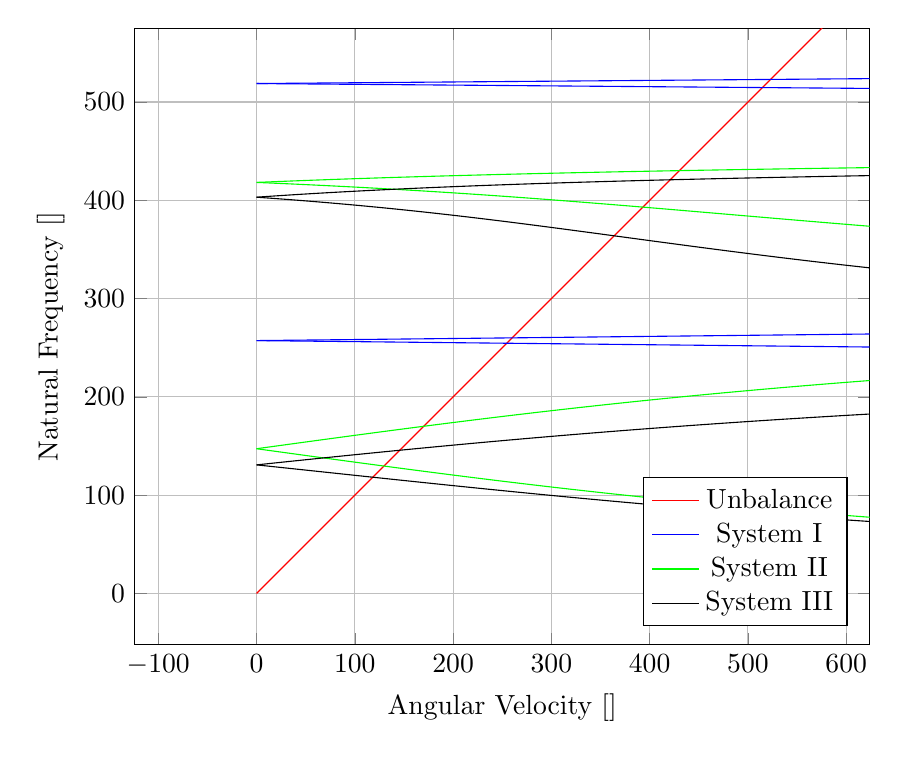
\begin{tikzpicture}
\begin{axis}[%
width=0.9\linewidth,
%height=0.9\linewidth,
xmax=500,
xmin=0,
xlabel={Angular Velocity [\si{\hertz}]},
ylabel={Natural Frequency [\si{\hertz}]},
grid=major,
legend pos=south east,
axis equal,
]
\addplot [color=red]
  table[row sep=crcr]{%
0	0\\
5	5\\
10	10\\
15	15\\
20	20\\
25	25\\
30	30\\
35	35\\
40	40\\
45	45\\
50	50\\
55	55\\
60	60\\
65	65\\
70	70\\
75	75\\
80	80\\
85	85\\
90	90\\
95	95\\
100	100\\
105	105\\
110	110\\
115	115\\
120	120\\
125	125\\
130	130\\
135	135\\
140	140\\
145	145\\
150	150\\
155	155\\
160	160\\
165	165\\
170	170\\
175	175\\
180	180\\
185	185\\
190	190\\
195	195\\
200	200\\
205	205\\
210	210\\
215	215\\
220	220\\
225	225\\
230	230\\
235	235\\
240	240\\
245	245\\
250	250\\
255	255\\
260	260\\
265	265\\
270	270\\
275	275\\
280	280\\
285	285\\
290	290\\
295	295\\
300	300\\
305	305\\
310	310\\
315	315\\
320	320\\
325	325\\
330	330\\
335	335\\
340	340\\
345	345\\
350	350\\
355	355\\
360	360\\
365	365\\
370	370\\
375	375\\
380	380\\
385	385\\
390	390\\
395	395\\
400	400\\
405	405\\
410	410\\
415	415\\
420	420\\
425	425\\
430	430\\
435	435\\
440	440\\
445	445\\
450	450\\
455	455\\
460	460\\
465	465\\
470	470\\
475	475\\
480	480\\
485	485\\
490	490\\
495	495\\
500	500\\
505	505\\
510	510\\
515	515\\
520	520\\
525	525\\
530	530\\
535	535\\
540	540\\
545	545\\
550	550\\
555	555\\
560	560\\
565	565\\
570	570\\
575	575\\
580	580\\
585	585\\
590	590\\
595	595\\
600	600\\
605	605\\
610	610\\
615	615\\
620	620\\
625	625\\
630	630\\
635	635\\
640	640\\
645	645\\
650	650\\
655	655\\
660	660\\
665	665\\
670	670\\
675	675\\
680	680\\
685	685\\
690	690\\
695	695\\
700	700\\
705	705\\
710	710\\
715	715\\
720	720\\
725	725\\
730	730\\
735	735\\
740	740\\
745	745\\
};
\addlegendentry{Unbalance}

\addplot [color=blue]
  table[row sep=crcr]{%
0	257.272586991077\\
5	257.216756305163\\
10	257.166122314727\\
15	257.115113452385\\
20	257.060285088651\\
25	257.006790700351\\
30	256.953798539078\\
35	256.900706325953\\
40	256.847882348684\\
45	256.794879138477\\
50	256.742532382384\\
55	256.689223408172\\
60	256.635850618845\\
65	256.583058553164\\
70	256.530018642645\\
75	256.47699236764\\
80	256.424003816099\\
85	256.371086173661\\
90	256.318116876878\\
95	256.265263191479\\
100	256.212319765853\\
105	256.159394682353\\
110	256.106752104767\\
115	256.053904622839\\
120	256.001041150304\\
125	255.948179779131\\
130	255.895431240398\\
135	255.842572540307\\
140	255.789661495036\\
145	255.736877230452\\
150	255.683959418278\\
155	255.631219413459\\
160	255.578409877976\\
165	255.525595660325\\
170	255.472849380452\\
175	255.420032040628\\
180	255.367247823351\\
185	255.314557456\\
190	255.261824507237\\
195	255.209027533111\\
200	255.156337577049\\
205	255.103646916983\\
210	255.05097839932\\
215	254.998312161035\\
220	254.945601851016\\
225	254.89291431462\\
230	254.840222127444\\
235	254.787605105338\\
240	254.73493260357\\
245	254.682319127622\\
250	254.629667800461\\
255	254.576984844884\\
260	254.524359435086\\
265	254.471844001447\\
270	254.419224724266\\
275	254.36665612185\\
280	254.314119482326\\
285	254.261582356509\\
290	254.209060912088\\
295	254.156497885873\\
300	254.103917115442\\
305	254.051426738989\\
310	253.998890147311\\
315	253.946435423718\\
320	253.893967788625\\
325	253.841492125426\\
330	253.788963802845\\
335	253.736492205133\\
340	253.684076970925\\
345	253.631700556921\\
350	253.579199966467\\
355	253.526812832744\\
360	253.474305751572\\
365	253.42198545965\\
370	253.369589224185\\
375	253.317210879281\\
380	253.264804116779\\
385	253.212472339583\\
390	253.16015523988\\
395	253.107793817576\\
400	253.055450943874\\
405	253.003114728444\\
410	252.950783914853\\
415	252.898505482253\\
420	252.846201228413\\
425	252.793908633072\\
430	252.74162843635\\
435	252.689403058539\\
440	252.63709690339\\
445	252.584841969055\\
450	252.53265104473\\
455	252.480423980978\\
460	252.428225846147\\
465	252.376023952813\\
470	252.323783055811\\
475	252.271581465921\\
480	252.219446918785\\
485	252.167281918348\\
490	252.115116109234\\
495	252.062986545162\\
500	252.010818678475\\
505	251.958701019062\\
510	251.906588852122\\
515	251.854491409917\\
520	251.80238160639\\
525	251.750276248531\\
530	251.698228550162\\
535	251.646125626471\\
540	251.594063256866\\
545	251.542032218959\\
550	251.489974349878\\
555	251.43796467612\\
560	251.385925740567\\
565	251.333893372762\\
570	251.281886309016\\
575	251.229975567328\\
580	251.177919587345\\
585	251.125961961362\\
590	251.074027360075\\
595	251.022048319568\\
600	250.970120457379\\
605	250.918198835664\\
610	250.866280950737\\
615	250.814339414972\\
620	250.762468557909\\
625	250.710594434505\\
630	250.658660864527\\
635	250.606825572877\\
640	250.554973768381\\
645	250.503079748869\\
650	250.4512487828\\
655	250.399394117994\\
660	250.347593152592\\
665	250.295742301692\\
670	250.243950719676\\
675	250.192169572187\\
680	250.140362795618\\
685	250.088615974885\\
690	250.036825857548\\
695	249.985083794921\\
700	249.933315581399\\
705	249.881633481997\\
710	249.829863184676\\
715	249.77814613184\\
720	249.726446144214\\
725	249.674741992092\\
730	249.623055710882\\
735	249.571388361496\\
740	249.519696356051\\
745	249.468024828992\\
};
\addlegendentry{System I}

\addplot [color=blue, forget plot]
  table[row sep=crcr]{%
0	257.272586991678\\
5	257.32318875337\\
10	257.378520396871\\
15	257.433736022089\\
20	257.485082668883\\
25	257.537785769627\\
30	257.590992830365\\
35	257.644100233949\\
40	257.69747405442\\
45	257.750670246285\\
50	257.804527292591\\
55	257.857414814236\\
60	257.910238207089\\
65	257.963648275598\\
70	258.016805617063\\
75	258.069976641877\\
80	258.123186267204\\
85	258.176468491851\\
90	258.229694872041\\
95	258.28304079911\\
100	258.336296219102\\
105	258.38956981736\\
110	258.443132287204\\
115	258.496484122984\\
120	258.549818154693\\
125	258.603156043906\\
130	258.656608235401\\
135	258.709947265627\\
140	258.763232444281\\
145	258.816648674979\\
150	258.869924916958\\
155	258.923386651969\\
160	258.976773695564\\
165	259.030157146567\\
170	259.083608721162\\
175	259.136986770483\\
180	259.19039917147\\
185	259.243907688037\\
190	259.297372149763\\
195	259.350771063142\\
200	259.404278819459\\
205	259.45778662604\\
210	259.511314527084\\
215	259.564845236061\\
220	259.618332381135\\
225	259.671840430029\\
230	259.725343785915\\
235	259.778922402504\\
240	259.83244551418\\
245	259.88602850883\\
250	259.939556719227\\
255	259.993066347048\\
260	260.046635473117\\
265	260.10031761741\\
270	260.153890913211\\
275	260.207517376141\\
280	260.261175014517\\
285	260.314831289872\\
290	260.368519424466\\
295	260.422146697615\\
300	260.475744325985\\
305	260.529446100188\\
310	260.583102043708\\
315	260.636841735359\\
320	260.690567820785\\
325	260.744284730834\\
330	260.797944116262\\
335	260.85166473043\\
340	260.9054416642\\
345	260.959260363744\\
350	261.012946670578\\
355	261.066751700558\\
360	261.12042964918\\
365	261.174303930184\\
370	261.228096292745\\
375	261.281907386223\\
380	261.335689001881\\
385	261.389548417645\\
390	261.443421736652\\
395	261.497247942817\\
400	261.551092425887\\
405	261.604942963693\\
410	261.658797908255\\
415	261.712708875078\\
420	261.766592755772\\
425	261.820485086567\\
430	261.874390681818\\
435	261.928355179252\\
440	261.982229879735\\
445	262.036160454569\\
450	262.0901564329\\
455	262.144115206768\\
460	262.198102888742\\
465	262.252087013453\\
470	262.306025810245\\
475	262.360007115338\\
480	262.414058894589\\
485	262.468077629632\\
490	262.522092511554\\
495	262.576147241797\\
500	262.630159227649\\
505	262.684224406054\\
510	262.738293755012\\
515	262.792378248858\\
520	262.846448070927\\
525	262.900522489443\\
530	262.954656590078\\
535	263.008729460318\\
540	263.062847945203\\
545	263.116996733271\\
550	263.171114032988\\
555	263.225285797228\\
560	263.279422070553\\
565	263.333562990593\\
570	263.387734778904\\
575	263.442006481675\\
580	263.496120732853\\
585	263.55033938918\\
590	263.604582382794\\
595	263.658776244684\\
600	263.713023326611\\
605	263.767278014891\\
610	263.821535648101\\
615	263.875762736236\\
620	263.930068931748\\
625	263.984368829717\\
630	264.038601594424\\
635	264.09294135351\\
640	264.147261213319\\
645	264.201534635613\\
650	264.255874779487\\
655	264.310188277114\\
660	264.364557924818\\
665	264.418873174279\\
670	264.473248815248\\
675	264.527639153555\\
680	264.581996035901\\
685	264.636421157372\\
690	264.690793360841\\
695	264.745218948886\\
700	264.799614775185\\
705	264.854102959176\\
710	264.908491749726\\
715	264.962938600759\\
720	265.017402632613\\
725	265.071861741121\\
730	265.126339144609\\
735	265.180833437148\\
740	265.235300632998\\
745	265.28978661919\\
};
\addplot [color=blue, forget plot]
  table[row sep=crcr]{%
0	518.821665977453\\
5	518.78558453498\\
10	518.741514550627\\
15	518.700751312816\\
20	518.659852156303\\
25	518.620042397766\\
30	518.580270986675\\
35	518.540870738576\\
40	518.50077036672\\
45	518.461011139881\\
50	518.422040908847\\
55	518.381859106328\\
60	518.342349590047\\
65	518.301686858617\\
70	518.261788576499\\
75	518.221972889584\\
80	518.182107620019\\
85	518.142103527475\\
90	518.102256206976\\
95	518.062159787043\\
100	518.022301292406\\
105	517.982414511259\\
110	517.943269733785\\
115	517.90327501769\\
120	517.863317873793\\
125	517.823393043221\\
130	517.783500985608\\
135	517.743526941726\\
140	517.703283465541\\
145	517.663319677564\\
150	517.623724691199\\
155	517.583696076342\\
160	517.543860584638\\
165	517.504029401468\\
170	517.464075436581\\
175	517.424307526636\\
180	517.384477921139\\
185	517.344443267144\\
190	517.304527127367\\
195	517.264807224166\\
200	517.224831581256\\
205	517.184885260127\\
210	517.144901411533\\
215	517.104944868159\\
220	517.065125442707\\
225	517.025261512638\\
230	516.985446971159\\
235	516.945467093764\\
240	516.905641120994\\
245	516.86570347409\\
250	516.825637379609\\
255	516.785906913326\\
260	516.746073105567\\
265	516.705977492349\\
270	516.666168293412\\
275	516.626251833317\\
280	516.586414092721\\
285	516.546447741534\\
290	516.506577557585\\
295	516.466775628609\\
300	516.426597388137\\
305	516.386674699898\\
310	516.346878509292\\
315	516.307029060585\\
320	516.267083192251\\
325	516.227190693619\\
330	516.187458364281\\
335	516.147607978865\\
340	516.10764442683\\
345	516.067590203371\\
350	516.027896085392\\
355	515.987932666367\\
360	515.94828949868\\
365	515.908199656497\\
370	515.868343993342\\
375	515.828452819239\\
380	515.788665016504\\
385	515.748716428428\\
390	515.708751888374\\
395	515.66891613624\\
400	515.6290676741\\
405	515.589231943915\\
410	515.549401352133\\
415	515.509474395464\\
420	515.469618949079\\
425	515.429770767964\\
430	515.389913872064\\
435	515.349946927465\\
440	515.310203379067\\
445	515.270361216757\\
450	515.230380554287\\
455	515.190524367992\\
460	515.150608790909\\
465	515.11073989488\\
470	515.070974460166\\
475	515.031147978421\\
480	514.991180919872\\
485	514.951314509181\\
490	514.911468885121\\
495	514.871565381276\\
500	514.831789003052\\
505	514.791893311319\\
510	514.752019171346\\
515	514.712133318357\\
520	514.672303788986\\
525	514.63249220188\\
530	514.592550289604\\
535	514.552785719906\\
540	514.51293392399\\
545	514.473036023459\\
550	514.433222933524\\
555	514.393320660539\\
560	514.353514521255\\
565	514.313717531102\\
570	514.273881715408\\
575	514.233832192074\\
580	514.194170349703\\
585	514.154286028785\\
590	514.114377695127\\
595	514.074590111562\\
600	514.03471283684\\
605	513.994843098689\\
610	513.954983093407\\
615	513.915210401837\\
620	513.87528072888\\
625	513.835393885634\\
630	513.795687993028\\
635	513.755749746744\\
640	513.715873631395\\
645	513.676131905172\\
650	513.636270773673\\
655	513.59648167198\\
660	513.556582967559\\
665	513.516844056985\\
670	513.476969678335\\
675	513.437102881036\\
680	513.397326252617\\
685	513.357415037909\\
690	513.317549307736\\
695	513.277682425144\\
700	513.237916873851\\
705	513.197953585915\\
710	513.158245250987\\
715	513.118428995463\\
720	513.078579743249\\
725	513.038778950939\\
730	512.998953008496\\
735	512.959108670901\\
740	512.919348133546\\
745	512.8795709902\\
};
\addplot [color=blue, forget plot]
  table[row sep=crcr]{%
0	518.821665977702\\
5	518.865507567108\\
10	518.901276110817\\
15	518.940644423583\\
20	518.97938094363\\
25	519.019432039367\\
30	519.059525625568\\
35	519.099998158819\\
40	519.139769619993\\
45	519.179881681912\\
50	519.220788866453\\
55	519.26047937891\\
60	519.300847868392\\
65	519.340052477696\\
70	519.380027651246\\
75	519.420088287963\\
80	519.460098474768\\
85	519.499966575482\\
90	519.539996544418\\
95	519.579772635221\\
100	519.61978901693\\
105	519.659773914085\\
110	519.700499868828\\
115	519.740378005554\\
120	519.78029738673\\
125	519.820245006711\\
130	519.860225552847\\
135	519.900125740357\\
140	519.939756117359\\
145	519.979663623156\\
150	520.019947185045\\
155	520.059788094977\\
160	520.09982791398\\
165	520.139870755099\\
170	520.179791003693\\
175	520.219896643281\\
180	520.259942529903\\
185	520.299780418661\\
190	520.339738195887\\
195	520.379892907511\\
200	520.419789958499\\
205	520.459715175477\\
210	520.499606189102\\
215	520.539522166004\\
220	520.579575023081\\
225	520.619585736787\\
230	520.659644930623\\
235	520.699538886211\\
240	520.739586836913\\
245	520.779520589816\\
250	520.819329004499\\
255	520.859472010869\\
260	520.899511920336\\
265	520.939287148447\\
270	520.979351216656\\
275	521.01930655894\\
280	521.05934412891\\
285	521.099249376058\\
290	521.139250155391\\
295	521.179324986162\\
300	521.219014060118\\
305	521.258967328999\\
310	521.299042029393\\
315	521.339067046927\\
320	521.378990963227\\
325	521.418970992593\\
330	521.459114413768\\
335	521.499134437715\\
340	521.539044241911\\
345	521.578858067317\\
350	521.619039234504\\
355	521.658947394017\\
360	521.699179689079\\
365	521.738957978982\\
370	521.778976426533\\
375	521.818956995386\\
380	521.859040837224\\
385	521.89896197308\\
390	521.938867522723\\
395	521.978904807318\\
400	522.018928176801\\
405	522.05896466705\\
410	522.09900665932\\
415	522.138951281786\\
420	522.178963830507\\
425	522.218988924671\\
430	522.25900383048\\
435	522.298905343817\\
440	522.339035605014\\
445	522.379065208487\\
450	522.418953683062\\
455	522.458968071637\\
460	522.498923284524\\
465	522.538923086479\\
470	522.579030187433\\
475	522.619074860438\\
480	522.658977328796\\
485	522.698978978444\\
490	522.739006079917\\
495	522.778970886861\\
500	522.819066010633\\
505	522.859038901296\\
510	522.899033797409\\
515	522.939017738097\\
520	522.979058868705\\
525	523.019115415391\\
530	523.059042814273\\
535	523.099149778818\\
540	523.13916559565\\
545	523.179136617646\\
550	523.219195151587\\
555	523.259159657842\\
560	523.299222616269\\
565	523.339299131266\\
570	523.379328889173\\
575	523.419145536941\\
580	523.459354821025\\
585	523.499338377764\\
590	523.539298675404\\
595	523.579378425806\\
600	523.619369742251\\
605	523.659366256801\\
610	523.699370951295\\
615	523.739470845206\\
620	523.779405499069\\
625	523.819384615964\\
630	523.859550112616\\
635	523.899476655875\\
640	523.939468214364\\
645	523.979594055705\\
650	524.019600903437\\
655	524.059677957022\\
660	524.099646565406\\
665	524.139774878142\\
670	524.179770613543\\
675	524.21976546784\\
680	524.259859727207\\
685	524.299807923306\\
690	524.339809043382\\
695	524.379807237106\\
700	524.419907596664\\
705	524.459807280264\\
710	524.499969047814\\
715	524.540018454664\\
720	524.580034050728\\
725	524.62009865794\\
730	524.660135188494\\
735	524.700156968001\\
740	524.740262595971\\
745	524.780353972661\\
};
\addplot [color=green]
  table[row sep=crcr]{%
0	147.243635606529\\
5	146.556929034497\\
10	145.870226144453\\
15	145.183565480321\\
20	144.497020772435\\
25	143.810653460489\\
30	143.124560753936\\
35	142.438784449493\\
40	141.753448022229\\
45	141.068505041038\\
50	140.384256707839\\
55	139.700649142517\\
60	139.0177084055\\
65	138.335479520391\\
70	137.654171987065\\
75	136.973736051567\\
80	136.294372434826\\
85	135.615957260473\\
90	134.938703399124\\
95	134.262640368648\\
100	133.587863921073\\
105	132.914432581398\\
110	132.242380212444\\
115	131.571805410464\\
120	130.902733163032\\
125	130.235255901257\\
130	129.569471292244\\
135	128.905347389691\\
140	128.243058533374\\
145	127.58260478703\\
150	126.92403169731\\
155	126.267398970743\\
160	125.612795655613\\
165	124.960256062301\\
170	124.30983173035\\
175	123.66159272741\\
180	123.01557186772\\
185	122.371812565112\\
190	121.730372045947\\
195	121.091360089192\\
200	120.454744510771\\
205	119.820566146531\\
210	119.18892021048\\
215	118.559837265263\\
220	117.933347164506\\
225	117.309468669867\\
230	116.688301774829\\
235	116.069827701973\\
240	115.454141560758\\
245	114.841201434232\\
250	114.231093022464\\
255	113.623849706979\\
260	113.019488808523\\
265	112.418044247496\\
270	111.819545913117\\
275	111.224009628654\\
280	110.631492107925\\
285	110.041989076696\\
290	109.455530878174\\
295	108.872135928363\\
300	108.291854455186\\
305	107.71468446405\\
310	107.140644299746\\
315	106.569760130946\\
320	106.00204113708\\
325	105.43750543642\\
330	104.876169530755\\
335	104.318043367474\\
340	103.763146071133\\
345	103.211492044891\\
350	102.663086074237\\
355	102.117917728489\\
360	101.576028464366\\
365	101.037407963788\\
370	100.502064133367\\
375	99.9700070812725\\
380	99.4412376133965\\
385	98.9157569064249\\
390	98.3935794563024\\
395	97.8746876165648\\
400	97.3590984767039\\
405	96.8468090905265\\
410	96.3378111505528\\
415	95.8321120812699\\
420	95.3297051513636\\
425	94.8305907938342\\
430	94.3347613008163\\
435	93.8422113327983\\
440	93.3529393260448\\
445	92.8669409357996\\
450	92.3842111342971\\
455	91.9047339445616\\
460	91.4285060333275\\
465	90.9555258044782\\
470	90.485772852519\\
475	90.0192442616835\\
480	89.5559308587307\\
485	89.0958272421979\\
490	88.6389089474763\\
495	88.1851740535295\\
500	87.7346092252898\\
505	87.2872028916842\\
510	86.842940734763\\
515	86.4018131124755\\
520	85.9638039339654\\
525	85.5288988434159\\
530	85.0970853502923\\
535	84.6683474152265\\
540	84.2426702490239\\
545	83.8200428239067\\
550	83.4004447658437\\
555	82.9838613616171\\
560	82.5702801150373\\
565	82.1596819027643\\
570	81.7520506771562\\
575	81.3473699243088\\
580	80.9456251517408\\
585	80.5467926326406\\
590	80.1508647623674\\
595	79.7578156416532\\
600	79.3676343384703\\
605	78.9802982299195\\
610	78.5957915103441\\
615	78.2140981813318\\
620	77.8351967737321\\
625	77.4590712745137\\
630	77.0857023393728\\
635	76.7150725578415\\
640	76.3471609266898\\
645	75.9819535634827\\
650	75.6194274017191\\
655	75.2595675787181\\
660	74.9023528811955\\
665	74.5477654054762\\
670	74.1957859513432\\
675	73.8463956807976\\
680	73.4995773310182\\
685	73.1553109224073\\
690	72.8135778479752\\
695	72.4743593053272\\
700	72.1376368061668\\
705	71.8033901241329\\
710	71.4716021603126\\
715	71.1422544183783\\
720	70.8153267804997\\
725	70.490801091945\\
730	70.1686602420114\\
735	69.8488834433355\\
740	69.5314537540011\\
745	69.2163510003807\\
};
\addlegendentry{System II}

\addplot [color=green, forget plot]
  table[row sep=crcr]{%
0	147.243635606758\\
5	147.930193998975\\
10	148.61660943431\\
15	149.302771611007\\
20	149.988607334787\\
25	150.674029885481\\
30	151.358993233954\\
35	152.043387653956\\
40	152.72719884439\\
45	153.410215201274\\
50	154.092631185835\\
55	154.774234842691\\
60	155.454897068255\\
65	156.13451019951\\
70	156.813183514079\\
75	157.490692800356\\
80	158.167139266229\\
85	158.842206899974\\
90	159.516014448534\\
95	160.188445554438\\
100	160.859476677991\\
105	161.529037074486\\
110	162.19701305804\\
115	162.863395100759\\
120	163.528061135981\\
125	164.190996512224\\
130	164.852204175635\\
135	165.511476595918\\
140	166.168930899041\\
145	166.824428705411\\
150	167.477891759974\\
155	168.129266916242\\
160	168.778564833091\\
165	169.425697148933\\
170	170.070609506263\\
175	170.713286103856\\
180	171.353648666987\\
185	171.991633192236\\
190	172.627208462206\\
195	173.260470856939\\
200	173.891214357555\\
205	174.519364808565\\
210	175.145018756456\\
215	175.768105809976\\
220	176.388561468548\\
225	177.006295479241\\
230	177.621425400787\\
235	178.233778224805\\
240	178.84347269604\\
245	179.450279928305\\
250	180.054304531576\\
255	180.655519967306\\
260	181.253866192436\\
265	181.849328808358\\
270	182.44188131747\\
275	183.03146996772\\
280	183.618163331813\\
285	184.201853233733\\
290	184.782540263491\\
295	185.360190169164\\
300	185.934880480738\\
305	186.506523878128\\
310	187.07510158013\\
315	187.640630227451\\
320	188.203068371845\\
325	188.76241660836\\
330	189.318668063937\\
335	189.871801055301\\
340	190.421833093628\\
345	190.968769019652\\
350	191.512582426847\\
355	192.053189373125\\
360	192.590721996159\\
365	193.125093046335\\
370	193.65631495243\\
375	194.184405416071\\
380	194.709346635953\\
385	195.231128901969\\
390	195.749805163203\\
395	196.265289837601\\
400	196.777659707154\\
405	197.286903339837\\
410	197.792979646086\\
415	198.295947208029\\
420	198.795783180799\\
425	199.292512657544\\
430	199.786121056651\\
435	200.276605901265\\
440	200.763995308646\\
445	201.248307603602\\
450	201.729557912351\\
455	202.207706858847\\
460	202.682777558576\\
465	203.154833376918\\
470	203.62380188182\\
475	204.089737928167\\
480	204.552659988592\\
485	205.012612607045\\
490	205.469506053091\\
495	205.923427811069\\
500	206.374377267556\\
505	206.822367984245\\
510	207.267404880539\\
515	207.709523290941\\
520	208.148719010118\\
525	208.585002127522\\
530	209.018396827578\\
535	209.44890942241\\
540	209.876551838631\\
545	210.301371824871\\
550	210.723344761104\\
555	211.142493784685\\
560	211.558862531998\\
565	211.972441067058\\
570	212.383253221305\\
575	212.791310963491\\
580	213.196651775148\\
585	213.599236678193\\
590	213.999162177825\\
595	214.396372973348\\
600	214.790944164611\\
605	215.18284713185\\
610	215.572118021545\\
615	215.958793464173\\
620	216.342856597386\\
625	216.724346606834\\
630	217.103270464343\\
635	217.479655371896\\
640	217.853491236596\\
645	218.224843230015\\
650	218.593684858253\\
655	218.960069155425\\
660	219.323991707111\\
665	219.685476224512\\
670	220.044533842354\\
675	220.401184218417\\
680	220.755459050193\\
685	221.107364657455\\
690	221.456920766256\\
695	221.804144687453\\
700	222.149056427138\\
705	222.491657558007\\
710	222.831984075107\\
715	223.170057926412\\
720	223.505877177927\\
725	223.839464709575\\
730	224.170860006015\\
735	224.500051409857\\
740	224.827078899775\\
745	225.151924868536\\
};
\addplot [color=green, forget plot]
  table[row sep=crcr]{%
0	418.208170844837\\
5	417.996240190607\\
10	417.780752339464\\
15	417.563490504093\\
20	417.343616735382\\
25	417.121410397931\\
30	416.896740821938\\
35	416.669403110155\\
40	416.439518844835\\
45	416.207075598458\\
50	415.972071517441\\
55	415.734148793872\\
60	415.493710402879\\
65	415.250783431045\\
70	415.004881488608\\
75	414.756432519737\\
80	414.505151071216\\
85	414.251000604269\\
90	413.994128713516\\
95	413.734478721729\\
100	413.47190384116\\
105	413.206400319661\\
110	412.938092858449\\
115	412.66682729699\\
120	412.392757399501\\
125	412.115710160731\\
130	411.835513482911\\
135	411.55247530664\\
140	411.266450418003\\
145	410.977419019596\\
150	410.685368261685\\
155	410.390370469031\\
160	410.092264327137\\
165	409.791136330592\\
170	409.487036763035\\
175	409.17978984153\\
180	408.869508433576\\
185	408.556315209345\\
190	408.240087526208\\
195	407.920539972447\\
200	407.598209537647\\
205	407.272790220232\\
210	406.94434079625\\
215	406.612857790779\\
220	406.278415567288\\
225	405.941085311674\\
230	405.600614366269\\
235	405.257337586214\\
240	404.910912912451\\
245	404.561821552384\\
250	404.209821184792\\
255	403.854836378601\\
260	403.497077604144\\
265	403.13659094052\\
270	402.773250970069\\
275	402.407270043357\\
280	402.038470615599\\
285	401.667106166417\\
290	401.293156019042\\
295	400.916703232638\\
300	400.537595262169\\
305	400.156032729006\\
310	399.772071138714\\
315	399.385702694091\\
320	398.997024829567\\
325	398.60609933713\\
330	398.212946272431\\
335	397.817660335719\\
340	397.420252799767\\
345	397.020770062713\\
350	396.619298954207\\
355	396.216051618409\\
360	395.810902661543\\
365	395.403939192083\\
370	394.995280506915\\
375	394.58496309545\\
380	394.173073592031\\
385	393.759710167891\\
390	393.344838239258\\
395	392.928694462843\\
400	392.511218356362\\
405	392.092521691475\\
410	391.672687144709\\
415	391.251774203796\\
420	390.829865553969\\
425	390.407013143399\\
430	389.983325316669\\
435	389.558873424849\\
440	389.13370552198\\
445	388.707895925824\\
450	388.281494764845\\
455	387.854669932161\\
460	387.42740329039\\
465	386.999777616579\\
470	386.571904842649\\
475	386.14381690024\\
480	385.71560167984\\
485	385.2873252747\\
490	384.859049844325\\
495	384.430834380087\\
500	384.002762299715\\
505	383.57488634104\\
510	383.147284988877\\
515	382.719985806896\\
520	382.29308863697\\
525	381.866647412062\\
530	381.440710899331\\
535	381.015346762999\\
540	380.590614374444\\
545	380.16653650169\\
550	379.743206640942\\
555	379.32066961895\\
560	378.898951339785\\
565	378.4781947443\\
570	378.058234178723\\
575	377.639327352106\\
580	377.221432737435\\
585	376.80464715757\\
590	376.38893638239\\
595	375.974411873878\\
600	375.561060094338\\
605	375.148960909394\\
610	374.738134285192\\
615	374.328602295889\\
620	373.920425441472\\
625	373.513621711706\\
630	373.10823079207\\
635	372.704279968678\\
640	372.301811986563\\
645	371.900823675737\\
650	371.501375372379\\
655	371.103466306868\\
660	370.707137182389\\
665	370.312407909918\\
670	369.919304789798\\
675	369.52784787863\\
680	369.138047073888\\
685	368.749929422098\\
690	368.363512185017\\
695	367.978812216369\\
700	367.595842122415\\
705	367.214628096035\\
710	366.835144018613\\
715	366.457454645964\\
720	366.08155758151\\
725	365.707459383202\\
730	365.335160652947\\
735	364.964684634748\\
740	364.59603461422\\
745	364.22921546498\\
};
\addplot [color=green, forget plot]
  table[row sep=crcr]{%
0	418.208170845272\\
5	418.41887140035\\
10	418.626081847182\\
15	418.831621066071\\
20	419.034718386527\\
25	419.235704936555\\
30	419.434495560264\\
35	419.630965144434\\
40	419.825270184973\\
45	420.0174541993\\
50	420.207571918488\\
55	420.395315861471\\
60	420.581147275375\\
65	420.765140392903\\
70	420.946863557047\\
75	421.126775313835\\
80	421.304678655925\\
85	421.480561298864\\
90	421.654630401638\\
95	421.826868627833\\
100	421.997177812785\\
105	422.16559943307\\
110	422.332303842491\\
115	422.497181564994\\
120	422.660429278354\\
125	422.821906688305\\
130	422.981485528751\\
135	423.139520340162\\
140	423.295891613225\\
145	423.450622151415\\
150	423.603728106729\\
155	423.75531769991\\
160	423.905259014693\\
165	424.053664798422\\
170	424.200608346404\\
175	424.345952498843\\
180	424.489825719555\\
185	424.632377442358\\
190	424.773501657996\\
195	424.912914080641\\
200	425.051198364448\\
205	425.188036749266\\
210	425.32350776072\\
215	425.457618469591\\
220	425.590450799091\\
225	425.72208591634\\
230	425.852253221121\\
235	425.98131101284\\
240	426.108890494308\\
245	426.23549927227\\
250	426.360870747098\\
255	426.484910608384\\
260	426.607830538543\\
265	426.729669140242\\
270	426.850268182929\\
275	426.96984153855\\
280	427.088157474013\\
285	427.205483579333\\
290	427.321758713191\\
295	427.437049305027\\
300	427.551138907955\\
305	427.664221857793\\
310	427.776318865906\\
315	427.887375446245\\
320	427.997476821434\\
325	428.106620045038\\
330	428.214783603408\\
335	428.322026889602\\
340	428.42830804087\\
345	428.533621530796\\
350	428.638006560211\\
355	428.741662510215\\
360	428.844367236028\\
365	428.946158850507\\
370	429.047113118066\\
375	429.147202872802\\
380	429.246460399269\\
385	429.344938700219\\
390	429.442505264159\\
395	429.539394125202\\
400	429.635437036638\\
405	429.730699113703\\
410	429.825203690052\\
415	429.91894296858\\
420	430.011939286877\\
425	430.104174404886\\
430	430.195704752791\\
435	430.286540705745\\
440	430.376620973791\\
445	430.466055747281\\
450	430.554717820411\\
455	430.64278836685\\
460	430.730158788303\\
465	430.816833988771\\
470	430.90290606053\\
475	430.988318101042\\
480	431.073095331336\\
485	431.157228428865\\
490	431.240776721881\\
495	431.323681096155\\
500	431.405997023797\\
505	431.487708197435\\
510	431.568847718119\\
515	431.649368107176\\
520	431.729332252119\\
525	431.808741488912\\
530	431.887587501115\\
535	431.965894048876\\
540	432.043672668518\\
545	432.120873131594\\
550	432.197568696049\\
555	432.273758075952\\
560	432.349400600715\\
565	432.424629270453\\
570	432.499179398057\\
575	432.573323131467\\
580	432.646946554717\\
585	432.720165510855\\
590	432.792813049184\\
595	432.865056803405\\
600	432.936777059853\\
605	433.008075800207\\
610	433.07891640828\\
615	433.149273465815\\
620	433.219211813846\\
625	433.288700416782\\
630	433.357764199472\\
635	433.426385228576\\
640	433.494623444941\\
645	433.5623956215\\
650	433.629790832241\\
655	433.696745358938\\
660	433.763305815861\\
665	433.829466102129\\
670	433.895247467653\\
675	433.960644300999\\
680	434.025639683953\\
685	434.090254591802\\
690	434.154498571605\\
695	434.218369603048\\
700	434.281866380915\\
705	434.345028616292\\
710	434.407766626201\\
715	434.470178096842\\
720	434.532262094178\\
725	434.594006377939\\
730	434.655377046782\\
735	434.716429043975\\
740	434.777139473737\\
745	434.837527713762\\
};
\addplot [color=black]
  table[row sep=crcr]{%
0	130.803903895619\\
5	130.276573284169\\
10	129.748476992757\\
15	129.219876509548\\
20	128.690840106557\\
25	128.161055708166\\
30	127.630943489819\\
35	127.100463761011\\
40	126.569621479213\\
45	126.03848042\\
50	125.507201653895\\
55	124.975750153557\\
60	124.444057054387\\
65	123.912307815972\\
70	123.380524403987\\
75	122.848785714771\\
80	122.317114745439\\
85	121.785557008025\\
90	121.254166243174\\
95	120.723031906455\\
100	120.192146539641\\
105	119.661626005079\\
110	119.131436010311\\
115	118.601697085719\\
120	118.072449562586\\
125	117.543719167486\\
130	117.015581903537\\
135	116.488053120412\\
140	115.961222494416\\
145	115.435134447831\\
150	114.909799798545\\
155	114.385281894818\\
160	113.861621867336\\
165	113.338905863959\\
170	112.817132184315\\
175	112.296362581399\\
180	111.776677212688\\
185	111.258085865506\\
190	110.740597575528\\
195	110.224351169728\\
200	109.709315736712\\
205	109.195508990753\\
210	108.683041987936\\
215	108.171938075671\\
220	107.662204790531\\
225	107.153913456389\\
230	106.647104921076\\
235	106.141783236123\\
240	105.638026099803\\
245	105.135822564585\\
250	104.635257709053\\
255	104.136330189039\\
260	103.639079735629\\
265	103.143561776671\\
270	102.649776819824\\
275	102.157780111697\\
280	101.667581876676\\
285	101.179231351348\\
290	100.692727431587\\
295	100.208138224701\\
300	99.7254918976935\\
305	99.2447716150982\\
310	98.7660192553957\\
315	98.2892703416997\\
320	97.8145453797171\\
325	97.3418665090394\\
330	96.8712487614912\\
335	96.4027221430597\\
340	95.936291456148\\
345	95.4719975276023\\
350	95.0098522597937\\
355	94.5498715177542\\
360	94.0920629200549\\
365	93.6364563201433\\
370	93.1830464563343\\
375	92.7318705370307\\
380	92.2829411041461\\
385	91.8362668616714\\
390	91.3918470881858\\
395	90.949709861512\\
400	90.5098536487509\\
405	90.0722981504767\\
410	89.6370520475605\\
415	89.2041224229448\\
420	88.7735167731116\\
425	88.3452291649982\\
430	87.9192947236326\\
435	87.4956946879432\\
440	87.0744470057392\\
445	86.6555547493536\\
450	86.2390148600961\\
455	85.824838255745\\
460	85.4130227986783\\
465	85.0035790374145\\
470	84.5964981127788\\
475	84.1917851048689\\
480	83.7894423994916\\
485	83.3894739975056\\
490	82.991868345572\\
495	82.5966366129513\\
500	82.2037703738872\\
505	81.8132675244862\\
510	81.4251322731929\\
515	81.0393514093962\\
520	80.6559310100952\\
525	80.2748598902475\\
530	79.8961409708293\\
535	79.5197709914107\\
540	79.1457343855335\\
545	78.7740368243035\\
550	78.4046613072508\\
555	78.0376145253539\\
560	77.6728859565968\\
565	77.3104672656032\\
570	76.9503502036759\\
575	76.5925304977168\\
580	76.2369996148269\\
585	75.8837501342443\\
590	75.5327705119365\\
595	75.1840602772768\\
600	74.8375993395776\\
605	74.4933923999748\\
610	74.1514181991442\\
615	73.8116758881726\\
620	73.4741492556414\\
625	73.1388365535029\\
630	72.8057239503934\\
635	72.4747964222721\\
640	72.1460478580664\\
645	71.8194694428927\\
650	71.4950516213707\\
655	71.1727771850663\\
660	70.8526418207705\\
665	70.5346332107361\\
670	70.218735158267\\
675	69.9049455094481\\
680	69.5932397542301\\
685	69.2836179397042\\
690	68.9760614764057\\
695	68.6705657542979\\
700	68.3671123667637\\
705	68.0656917362538\\
710	67.7662918243856\\
715	67.4689010706449\\
720	67.1735058248694\\
725	66.8800970219982\\
730	66.5886597179132\\
735	66.2991810275753\\
740	66.0116496932902\\
745	65.7260554219829\\
};
\addlegendentry{System III}

\addplot [color=black, forget plot]
  table[row sep=crcr]{%
0	130.803903896033\\
5	131.330690962876\\
10	131.856614318957\\
15	132.381841214025\\
20	132.906349279923\\
25	133.429707120885\\
30	133.952260050874\\
35	134.473866587815\\
40	134.994437133056\\
45	135.513934140389\\
50	136.032434879865\\
55	136.549812145612\\
60	137.06587759837\\
65	137.58074469884\\
70	138.094337317583\\
75	138.606646789618\\
80	139.117602656334\\
85	139.62715455068\\
90	140.135268461166\\
95	140.641958098396\\
100	141.147106139101\\
105	141.650768138938\\
110	142.152787356263\\
115	142.653229473975\\
120	143.152048541384\\
125	143.649173944809\\
130	144.14461580018\\
135	144.638280021748\\
140	145.130215668803\\
145	145.620383108735\\
150	146.108690734732\\
155	146.595135950015\\
160	147.079679969419\\
165	147.562368595976\\
170	148.043089829987\\
175	148.521850609566\\
180	148.998686185732\\
185	149.473517396045\\
190	149.946249465829\\
195	150.417052731529\\
200	150.885753796223\\
205	151.352299922612\\
210	151.816797925876\\
215	152.279204324622\\
220	152.739429976901\\
225	153.197530510551\\
230	153.653496708617\\
235	154.107241080663\\
240	154.558835583595\\
245	155.008166603892\\
250	155.455337217593\\
255	155.900249894426\\
260	156.342908511765\\
265	156.783361880929\\
270	157.22151979201\\
275	157.657435102668\\
280	158.091048193024\\
285	158.522408433172\\
290	158.951419928507\\
295	159.378194105046\\
300	159.802732014947\\
305	160.224904452218\\
310	160.644754522648\\
315	161.062313940528\\
320	161.477569097288\\
325	161.890518912359\\
330	162.301139026861\\
335	162.709457466141\\
340	163.115423702036\\
345	163.519108541654\\
350	163.920492309939\\
355	164.319567924605\\
360	164.716307770551\\
365	165.110760152164\\
370	165.502851899335\\
375	165.892670912751\\
380	166.280216551647\\
385	166.665475706719\\
390	167.048405577469\\
395	167.42907241894\\
400	167.807431299362\\
405	168.183529766253\\
410	168.557369090903\\
415	168.928950916666\\
420	169.298279174943\\
425	169.665301444574\\
430	170.030152748422\\
435	170.392728955497\\
440	170.753096074922\\
445	171.111255336919\\
450	171.467179436317\\
455	171.820912633423\\
460	172.172441548252\\
465	172.52181608387\\
470	172.868989720532\\
475	173.213993505292\\
480	173.556845197705\\
485	173.897576111098\\
490	174.236136029268\\
495	174.572601468695\\
500	174.906944101464\\
505	175.239172567079\\
510	175.569336366019\\
515	175.897382801046\\
520	176.223381964448\\
525	176.547295108259\\
530	176.869179236544\\
535	177.189053239434\\
540	177.506860038579\\
545	177.822680435818\\
550	178.136452165852\\
555	178.448270335362\\
560	178.758119480957\\
565	179.066000002756\\
570	179.371912617824\\
575	179.675891137577\\
580	179.977940098985\\
585	180.278076050323\\
590	180.576285858411\\
595	180.872638496193\\
600	181.167059335685\\
605	181.459667196648\\
610	181.750377878555\\
615	182.039269903345\\
620	182.32630699719\\
625	182.611555751036\\
630	182.895006525897\\
635	183.176628529426\\
640	183.456463429711\\
645	183.734546279258\\
650	184.010895055693\\
655	184.285460153619\\
660	184.558328434873\\
665	184.829480132775\\
670	185.098902691334\\
675	185.366659956984\\
680	185.632703223109\\
685	185.89709801101\\
690	186.159803278661\\
695	186.420899497879\\
700	186.68036187263\\
705	186.938191232102\\
710	187.194412883301\\
715	187.449043025791\\
720	187.70207722367\\
725	187.953561443488\\
730	188.203476938606\\
735	188.451829426034\\
740	188.698643840538\\
745	188.943956870723\\
};
\addplot [color=black, forget plot]
  table[row sep=crcr]{%
0	403.171424503726\\
5	402.820115671006\\
10	402.463899723504\\
15	402.102390667794\\
20	401.736068743526\\
25	401.36431534114\\
30	400.987438198565\\
35	400.605310745489\\
40	400.217837999288\\
45	399.824994368896\\
50	399.426627651883\\
55	399.022770704665\\
60	398.613386654043\\
65	398.198282564663\\
70	397.777567989739\\
75	397.351270373986\\
80	396.91908011217\\
85	396.481191724842\\
90	396.037608832101\\
95	395.587954076726\\
100	395.132637342163\\
105	394.671211451821\\
110	394.204144952438\\
115	393.731043656573\\
120	393.25195394217\\
125	392.766980068375\\
130	392.276017815954\\
135	391.779277640947\\
140	391.276459986903\\
145	390.767620522539\\
150	390.253017100706\\
155	389.732563086075\\
160	389.206345274049\\
165	388.674167817308\\
170	388.13635632241\\
175	387.592780799394\\
180	387.043510687054\\
185	386.488571541021\\
190	385.928342556933\\
195	385.362311562059\\
200	384.791089635597\\
205	384.214655909916\\
210	383.632900045058\\
215	383.04597347464\\
220	382.45414797854\\
225	381.857367857781\\
230	381.255705316952\\
235	380.64946064199\\
240	380.03861394151\\
245	379.423439828919\\
250	378.803856122774\\
255	378.180202522293\\
260	377.552570379944\\
265	376.920973240914\\
270	376.285746411417\\
275	375.646907687848\\
280	375.004739911026\\
285	374.359343502581\\
290	373.710977156881\\
295	373.059565752074\\
300	372.405306178588\\
305	371.748622557031\\
310	371.089585711369\\
315	370.428305910114\\
320	369.764972702946\\
325	369.099762775155\\
330	368.432886807505\\
335	367.764477464212\\
340	367.094789023364\\
345	366.423884392479\\
350	365.75195472926\\
355	365.079223276676\\
360	364.405877355356\\
365	363.732018772969\\
370	363.057937929265\\
375	362.383677405615\\
380	361.70937794916\\
385	361.0352496584\\
390	360.361519904291\\
395	359.688251056918\\
400	359.015663529004\\
405	358.343845437912\\
410	357.672950696369\\
415	357.003124478278\\
420	356.334516435551\\
425	355.667323827901\\
430	355.001531082447\\
435	354.337401924384\\
440	353.675028656427\\
445	353.01437712561\\
450	352.355774155416\\
455	351.69923732886\\
460	351.044894074735\\
465	350.392809827197\\
470	349.743132079099\\
475	349.095938085189\\
480	348.451308625531\\
485	347.809315795699\\
490	347.170092614712\\
495	346.533664668506\\
500	345.900138347493\\
505	345.269586028233\\
510	344.642049496191\\
515	344.01763539874\\
520	343.396367466829\\
525	342.778333802886\\
530	342.163560288671\\
535	341.552102091921\\
540	340.944068886422\\
545	340.339368779692\\
550	339.7381676064\\
555	339.140455859443\\
560	338.546270594263\\
565	337.955652107009\\
570	337.368633281539\\
575	336.785232512886\\
580	336.205478106914\\
585	335.629390460724\\
590	335.057000111545\\
595	334.488302828674\\
600	333.923344861416\\
605	333.362103853249\\
610	332.804622308239\\
615	332.25088904708\\
620	331.700924284729\\
625	331.154721590023\\
630	330.612288783535\\
635	330.073642924106\\
640	329.538763445445\\
645	329.007658595898\\
650	328.480319837266\\
655	327.956753689305\\
660	327.436951306424\\
665	326.920894471405\\
670	326.408588281911\\
675	325.90001755248\\
680	325.395177636231\\
685	324.894052262891\\
690	324.396632987894\\
695	323.902901463743\\
700	323.412846353679\\
705	322.926453347546\\
710	322.44370621134\\
715	321.964582926984\\
720	321.48908013958\\
725	321.017166341781\\
730	320.548818844856\\
735	320.084043863324\\
740	319.622795919381\\
745	319.165064342975\\
};
\addplot [color=black, forget plot]
  table[row sep=crcr]{%
0	403.171424504001\\
5	403.517866425882\\
10	403.859528831973\\
15	404.196161895155\\
20	404.528354985015\\
25	404.855649574052\\
30	405.178455604435\\
35	405.4967823631\\
40	405.810638254215\\
45	406.120149451482\\
50	406.425309145562\\
55	406.726202009613\\
60	407.022946591543\\
65	407.315456972108\\
70	407.603952468493\\
75	407.888571516853\\
80	408.169106355217\\
85	408.445856102313\\
90	408.71893362829\\
95	408.988013489802\\
100	409.253645579971\\
105	409.515421239113\\
110	409.773936665536\\
115	410.028838742835\\
120	410.280246740331\\
125	410.528340716246\\
130	410.773065570869\\
135	411.014736518362\\
140	411.25301656053\\
145	411.488025803306\\
150	411.720095428681\\
155	411.949147943309\\
160	412.175308862695\\
165	412.398353729929\\
170	412.618674406752\\
175	412.83609261747\\
180	413.050711911938\\
185	413.262505856287\\
190	413.471918062534\\
195	413.678279188036\\
200	413.88229088673\\
205	414.083879174876\\
210	414.282820401396\\
215	414.479242890321\\
220	414.67339856646\\
225	414.865134701712\\
230	415.054420348102\\
235	415.241546851346\\
240	415.426341548862\\
245	415.609078441183\\
250	415.789475622523\\
255	415.967856991726\\
260	416.14418535477\\
265	416.318311938213\\
270	416.490538862676\\
275	416.660699870414\\
280	416.82902369339\\
285	416.995321766098\\
290	417.159960620227\\
295	417.322561169107\\
300	417.483149494096\\
305	417.642162162481\\
310	417.799476529478\\
315	417.955014526804\\
320	418.108830416031\\
325	418.260955222701\\
330	418.411491938937\\
335	418.560375567758\\
340	418.707795076375\\
345	418.853556295715\\
350	418.997737950962\\
355	419.140411249679\\
360	419.281683569556\\
365	419.421429465712\\
370	419.559915710979\\
375	419.696918199891\\
380	419.83243143878\\
385	419.966560741151\\
390	420.099479474897\\
395	420.231014005824\\
400	420.361334912432\\
405	420.49033334468\\
410	420.618048184042\\
415	420.744520743387\\
420	420.869756492682\\
425	420.993972174744\\
430	421.116810771628\\
435	421.238620210059\\
440	421.359311699684\\
445	421.478702642806\\
450	421.59710710931\\
455	421.714420004569\\
460	421.830694994309\\
465	421.945847184797\\
470	422.060037462793\\
475	422.173234353836\\
480	422.285391326425\\
485	422.39650572625\\
490	422.506751908416\\
495	422.61595748331\\
500	422.724247370097\\
505	422.831637403603\\
510	422.938040833892\\
515	423.043636729359\\
520	423.148284100884\\
525	423.25212719378\\
530	423.355062471624\\
535	423.457093541914\\
540	423.558450210138\\
545	423.658799500584\\
550	423.758496674777\\
555	423.857317193533\\
560	423.955306555893\\
565	424.052574793149\\
570	424.149092696001\\
575	424.244769073516\\
580	424.339824680833\\
585	424.434105590872\\
590	424.52769939936\\
595	424.620529763021\\
600	424.712724202946\\
605	424.804119398136\\
610	424.894943937405\\
615	424.985072153744\\
620	425.074510879001\\
625	425.163277546948\\
630	425.251367701576\\
635	425.33898233341\\
640	425.425877068084\\
645	425.512162197953\\
650	425.597801318865\\
655	425.682887657352\\
660	425.767348051013\\
665	425.85121277081\\
670	425.934552846958\\
675	426.017263337855\\
680	426.099475555951\\
685	426.18109494511\\
690	426.262249707801\\
695	426.342782348326\\
700	426.422774455533\\
705	426.502283502697\\
710	426.581274292349\\
715	426.659736819002\\
720	426.737737256468\\
725	426.815182458035\\
730	426.892147341856\\
735	426.968688915914\\
740	427.044745592705\\
745	427.120272612166\\
};
\end{axis}

\end{tikzpicture}%
    \caption{Campbell diagram of system (I), (II) and (III)}
    \label{fig:campbell_diagram}
\end{figure}
The natural frequencies, in a campbell diagram, is split up in two lines as the angulare velocity is increased. This is a result of the gyroscopic effect. The upper line is the forward line and the lower line is the backward line. However, as there is no unbalance in the system, only the upper (forward) line is of interrest. From figure \ref{fig:campbell_diagram} it can be seen that the first critical speed of system (I) is $\approx \SI{260}{\hertz}$, system (II) is $\approx \SI{175}{\hertz}$ and system (III) is $\approx \SI{145}{\hertz}$.

The natural frequency at $\Omega = 0$ is lower for the heavier system (II) and (III). With system (III) having the lowest natural frequency. When increasing the angular velocity, the system (I) with the lowest moment of inertia, have an almost constant natural frequency. While the two other systems have a natural frequency that increases with the angular velocity. This is especially prevellent for the first natural frequency.

\subsubsection{First mode shapes}
The first mode shape of system (I), (II) and (III) is shown in figure \ref{fig:first_mode_shape}. The mode shape is normalized to 1 between the two bearings.
\begin{figure}[ht]
    \centering
    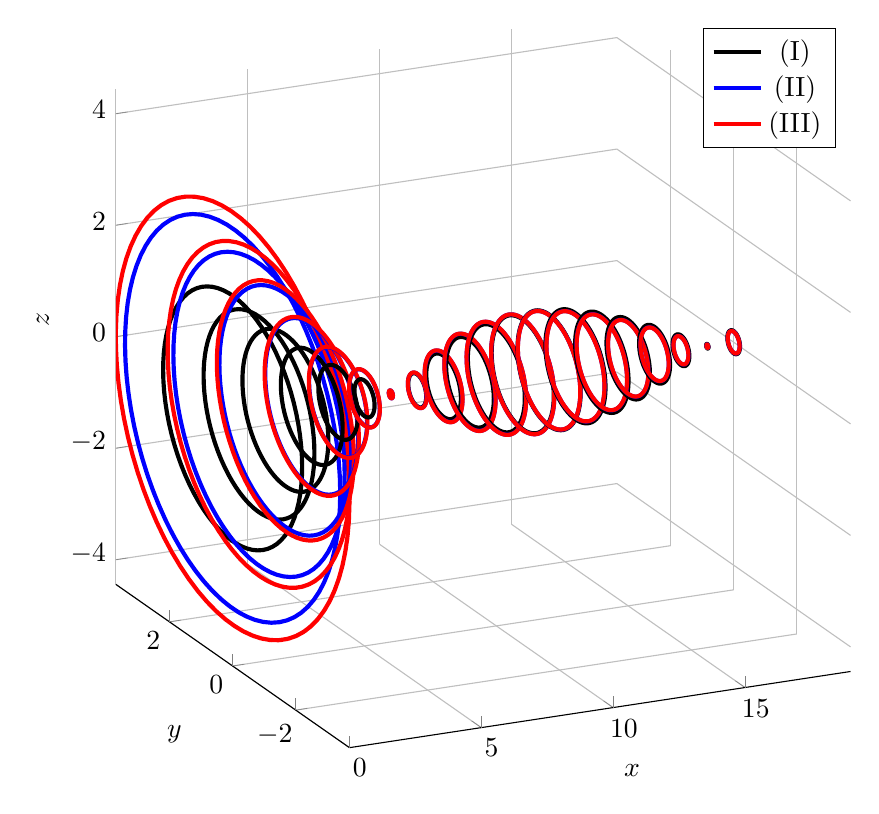
\begin{tikzpicture}

\begin{axis}[%
width=0.9\linewidth,
height=0.9\linewidth,
view={-25}{20},
axis x line*=bottom,
axis y line*=left,
axis z line*=left,
xmajorgrids,
ymajorgrids,
zmajorgrids,
xlabel={$x$},
ylabel={$y$},
zlabel={$z$},
]
\addplot3 [color=black, line width=1.5pt]
 table[row sep=crcr] {%
0	2.20144334269997	0\\
0	2.19425960010635	-0.177700809295844\\
0	2.17275525625534	-0.35424187321201\\
0	2.13707065695361	-0.528471015323349\\
0	2.08743869393266	-0.6992511477158\\
0	2.02418328490579	-0.86546769206939\\
0	1.94771725955367	-1.02603585383476\\
0	1.85853966523549	-1.17990770202911\\
0	1.75723251000959	-1.32607900844597\\
0	1.6444569642199	-1.46359580164352\\
0	1.52094904543826	-1.59156059293742\\
0	1.3875148149242	-1.70913823376502\\
0	1.24502511695211	-1.81556136619339\\
0	1.09440989533896	-1.910135430999\\
0	0.936652124265149	-1.99224320063442\\
0	0.772781392998376	-2.06134880749812\\
0	0.60386718638907	-2.11700124121716\\
0	0.431011904991588	-2.15883729211834\\
0	0.255343670364566	-2.18658392167735\\
0	0.0780089625058859	-2.20006004447562\\
0	-0.0998348625267575	-2.19917771003497\\
0	-0.277027125976733	-2.18394267681701\\
0	-0.452411401434586	-2.1544543746412\\
0	-0.624843062131669	-2.1109052557667\\
0	-0.793196751224666	-2.05357953887322\\
0	-0.95637372631701	-1.98285135413815\\
0	-1.11330903028395	-1.89918230151586\\
0	-1.26297844160165	-1.80311843815478\\
0	-1.40440515881973	-1.69528671461371\\
0	-1.53666617555174	-1.57639088313585\\
0	-1.6588983043779	-1.44720690468484\\
0	-1.77030381034578	-1.30857788471827\\
0	-1.87015561730231	-1.16140857074985\\
0	-1.95780205307881	-1.00665944761127\\
0	-2.03267110255989	-0.845340468950345\\
0	-2.09427414087904	-0.678504465876275\\
0	-2.14220912237679	-0.50724027576969\\
0	-2.17616320450876	-0.332665636101608\\
0	-2.1959147895792	-0.155919889639046\\
0	-2.20133497097469	0.0218434513540375\\
0	-2.19238837445944	0.199464233391513\\
0	-2.16913338904143	0.375783233383068\\
0	-2.13172178590278	0.549649724180073\\
0	-2.08039772788136	0.719928984673596\\
0	-2.015496175968	0.885509705430689\\
0	-1.93744070321939	1.04531124153689\\
0	-1.84674073035362	1.19829066530999\\
0	-1.74398820107025	1.34344957285634\\
0	-1.62985371879284	1.47984060004735\\
0	-1.5050821700473	1.60657360539048\\
0	-1.37048786303934	1.72282147944271\\
0	-1.22694921315886	1.82782554285214\\
0	-1.07540301009559	1.92090049779784\\
0	-0.916838303981075	2.00143890051302\\
0	-0.752289950458494	2.06891512570196\\
0	-0.582831856807657	2.12288879697745\\
0	-0.409569973203694	2.16300766093032\\
0	-0.233635074851172	2.18900988607376\\
0	-0.0561753821003419	2.20072577165856\\
0	0.121650933290538	2.19807885520698\\
0	0.29868330683964	2.18108641153693\\
0	0.473766355641899	2.14985934001976\\
0	0.645757418852307	2.10460144080727\\
0	0.813534015140056	2.04560808475183\\
0	0.976001168443222	1.97326428569995\\
0	1.13209855421326	1.88804218774051\\
0	1.28080741951008	1.79049798380673\\
0	1.42115723178446	1.68126828574227\\
0	1.5522320129552	1.56106596952195\\
0	1.67317631744243	1.43067552274274\\
0	1.78320081514188	1.2909479247491\\
0	1.88158744290368	1.14279509280709\\
0	1.96769409089489	0.987183930573533\\
0	2.04095879326088	0.825130017702473\\
0	2.10090339573548	0.657690981772846\\
0	2.14713667626389	0.485959595794901\\
0	2.17935689827161	0.311056646343681\\
0	2.19735377991606	0.134123618864991\\
0	2.20100986646862	-0.0436847521076363\\
0	2.19030129687031	-0.22120801920471\\
0	2.16529795945853	-0.397287595756778\\
0	2.12616303584823	-0.570774317186752\\
0	2.07315193594454	-0.740535940909972\\
0	2.00661063103721	-0.905464535794662\\
0	1.92697339585595	-1.06448371295632\\
0	1.83475997432268	-1.21655565069494\\
0	1.73057218749827	-1.3606878677277\\
0	1.61509000586155	-1.49593970051215\\
0	1.48906711155456	-1.62142844238653\\
0	1.35332597955636	-1.73633510446067\\
0	1.20875250988785	-1.83990976065958\\
0	1.05629024587972	-1.93147644203605\\
0	0.896934216237577	-2.01043754840988\\
0	0.731724441093217	-2.0762777485417\\
0	0.561739144424111	-2.12856734338734\\
0	0.388087717139669	-2.16696507048285\\
0	0.211903476759736	-2.19122033115755\\
0	0.0343362709387177	-2.20117482603952\\
0	-0.143455026892547	-2.19676358817958\\
0	-0.320310080790593	-2.17801540705116\\
};
\addlegendentry{(I)}
 \addplot3 [color=blue, line width=1.5pt]
 table[row sep=crcr] {%
0	3.40827651465001	0\\
0	3.39715463806375	-0.27511649954073\\
0	3.36386159404634	-0.548437480589001\\
0	3.30861466609878	-0.818179142912296\\
0	3.23177441740412	-1.08258104632002\\
0	3.13384233765027	-1.33991759998863\\
0	3.01545757011107	-1.58850932434614\\
0	2.87739274034586	-1.8267338120164\\
0	2.72054891374119	-2.05303631628779\\
0	2.54594971480363	-2.26593989800186\\
0	2.35473464658367	-2.46405506463921\\
0	2.14815165383051	-2.6460888386942\\
0	1.92754897841383	-2.81085319615476\\
0	1.69436636016696	-2.95727282001443\\
0	1.45012564057844	-3.08439211821407\\
0	1.19642083065585	-3.19138146021153\\
0	0.934907707782942	-3.27754259147691\\
0	0.667293009465199	-3.34231319057631\\
0	0.39532329448948	-3.38527053910262\\
0	0.120773544194392	-3.40613428050218\\
0	-0.15456442175611	-3.40476824979192\\
0	-0.428893639492664	-3.38118136222557\\
0	-0.70042372863354	-3.33552755510924\\
0	-0.967382577011251	-3.268104783146\\
0	-1.22802790617362	-3.17935307386628\\
0	-1.48065864217829	-3.06985165583511\\
0	-1.72362601747035	-2.94031517837871\\
0	-1.95534433138797	-2.79158904750184\\
0	-2.17430129906866	-2.62464390843569\\
0	-2.37906792121509	-2.4405693108253\\
0	-2.56830781030666	-2.24056659790001\\
0	-2.74078591239005	-2.02594106603499\\
0	-2.8953765675272	-1.79809344587366\\
0	-3.0310708562948	-1.55851076060853\\
0	-3.14698318438931	-1.30875662108297\\
0	-3.24235706236372	-1.05046102105174\\
0	-3.31657004277529	-0.785309699200653\\
0	-3.36913778252232	-0.515033137352771\\
0	-3.39971720385784	-0.241395266663396\\
0	-3.40810873344985	0.0338180444885096\\
0	-3.39425760487546	0.308810645779831\\
0	-3.35825421604804	0.581787827326819\\
0	-3.30033353924494	0.850968032667739\\
0	-3.22087358758595	1.1145944859011\\
0	-3.12039294797098	1.37094665709624\\
0	-2.99954739657799	1.61835149114838\\
0	-2.85912561900971	1.85519432679436\\
0	-2.70004406302112	2.07992943452716\\
0	-2.523340957421	2.29109010463466\\
0	-2.33016953618225	2.48729821952418\\
0	-2.12179051198342	2.66727324785991\\
0	-1.89956384830185	2.82984060181416\\
0	-1.6649398837571	2.97393930288953\\
0	-1.41944986663057	3.0986289062819\\
0	-1.16469596133701	3.20309563859316\\
0	-0.902340792069219	3.28665770883648\\
0	-0.634096591858657	3.34876975807251\\
0	-0.36171402786916	3.38902641863629\\
0	-0.0869707758543842	3.40716495972613\\
0	0.188340081653373	3.40306700208811\\
0	0.462421757705115	3.3767592906057\\
0	0.733485487473512	3.32841351975211\\
0	0.99976220243579	3.25834521304465\\
0	1.25951407601075	3.16701166381408\\
0	1.51104586529864	3.05500895072854\\
0	1.75271597490309	2.92306804754963\\
0	1.98294717062843	2.77205005251017\\
0	2.20023687313043	2.60294056844836\\
0	2.40316696434015	2.41684327037603\\
0	2.59041304266026	2.21497270246136\\
0	2.76075306653082	1.99864635143589\\
0	2.91307532995318	1.76927604815789\\
0	3.04638571792063	1.52835875344886\\
0	3.15981419440395	1.27746678833834\\
0	3.25262048054878	1.01823757247843\\
0	3.32419888602658	0.752362937699057\\
0	3.37408226200801	0.481578086447996\\
0	3.4019450499599	0.207650267177116\\
0	3.4076054063683	-0.0676327594161301\\
0	3.39102638952082	-0.34247438801823\\
0	3.3523162006027	-0.615080894052591\\
0	3.29172747753341	-0.883673140231681\\
0	3.20965564615212	-1.14649818790677\\
0	3.10663633951321	-1.4018407374351\\
0	2.98334190213421	-1.64803432290001\\
0	2.84057700201104	-1.88347218812309\\
0	2.67927337903817	-2.10661777298691\\
0	2.50048376410753	-2.31601474163086\\
0	2.30537500857265	-2.51029648707173\\
0	2.09522046891774	-2.68819505021848\\
0	1.87139169633241	-2.84854939507202\\
0	1.6353494854291	-2.99031298610282\\
0	1.38863434052283	-3.11256061835341\\
0	1.13285642169411	-3.2144944556899\\
0	0.869685036250887	-3.29544923779439\\
0	0.600837744172435	-3.35489662191547\\
0	0.328069148637333	-3.39244863104088\\
0	0.0531594447929611	-3.40786018598808\\
0	-0.222097198498272	-3.40103070488736\\
0	-0.495904348110677	-3.37200475961876\\
};
\addlegendentry{(II)}
 \addplot3 [color=red, line width=1.5pt]
 table[row sep=crcr] {%
0	6.28661281415439e-06	-3.70115186664535\\
0	-0.298751074067591	-3.68907478764803\\
0	-0.595558667725567	-3.65292135549722\\
0	-0.888479411256302	-3.59292752171204\\
0	-1.1756015886678	-3.50948482965019\\
0	-1.4550513276914	-3.40313785914207\\
0	-1.72500482940932	-3.27458067234856\\
0	-1.98370027108374	-3.12465228403835\\
0	-2.22944930450502	-2.95433118584754\\
0	-2.46064807481623	-2.76472896025836\\
0	-2.67578768790079	-2.55708302597461\\
0	-2.87346405801904	-2.33274856204048\\
0	-3.05238707142402	-2.09318966340907\\
0	-3.21138900615129	-1.8399697856828\\
0	-3.34943215303176	-1.57474154138719\\
0	-3.46561558818994	-1.29923591437143\\
0	-3.55918105282748	-1.01525096272695\\
0	-3.62951790191839	-0.724640083953036\\
0	-3.67616708951868	-0.429299918955692\\
0	-3.69882416468069	-0.131157973823085\\
0	-3.69734125841983	0.167839959837387\\
0	-3.67172804876564	0.465742503900487\\
0	-3.62215169759922	0.760605429184367\\
0	-3.54893575968903	1.05050434425495\\
0	-3.45255807104521	1.3335472547614\\
0	-3.33364763037379	1.60788691133547\\
0	-3.19298049398373	1.87173286546745\\
0	-3.03147471093824	2.12336315467747\\
0	-2.85018433150539	2.36113554071994\\
0	-2.65029252801153	2.58349822747632\\
0	-2.43310387299326	2.78899998858695\\
0	-2.2000358250439	2.97629963872519\\
0	-1.95260947792114	3.14417478670033\\
0	-1.69243963329092	3.29152981326338\\
0	-1.42122426189652	3.4174030215492\\
0	-1.1407334219336	3.5209729134886\\
0	-0.852797706954223	3.60156355122778\\
0	-0.559296298693197	3.65864896856472\\
0	-0.262144702788958	3.69185660361145\\
0	0.0367177525597138	3.70096973027951\\
0	0.335340573412337	3.68592887271964\\
0	0.631774829777406	3.64683219348456\\
0	0.924085875096138	3.58393485288154\\
0	1.21036597250689	3.4976473436959\\
0	1.48874674548633	3.38853281215356\\
0	1.75741137160953	3.25730338260735\\
0	2.0146064398478	3.10481550993327\\
0	2.2586533940187	2.93206438996916\\
0	2.48795948770399	2.74017746447517\\
0	2.70102817913926	2.53040706300537\\
0	2.89646889823409	2.30412222971245\\
0	3.07300612197951	2.06279978842713\\
0	3.22948769901284	1.80801470432487\\
0	3.36489236901068	1.54142980508367\\
0	3.4783364278355	1.26478492861654\\
0	3.56907949493645	0.979885568204945\\
0	3.63652934536404	0.688591089139455\\
0	3.68024577486313	0.392802593770487\\
0	3.69994347281906	0.0944505141665512\\
0	3.69549388430691	-0.20451798664473\\
0	3.66692604909157	-0.50215172262848\\
0	3.61442641210272	-0.796508218950101\\
0	3.53833760662198	-1.08566638933013\\
0	3.43915621812328	-1.36773907380897\\
0	3.31752954336074	-1.64088535509503\\
0	3.17425136585542	-1.90332257311517\\
0	3.01025677535189	-2.15333795935551\\
0	2.82661606505467	-2.38929981506244\\
0	2.62452774647383	-2.60966816035056\\
0	2.4053107274674	-2.81300478471712\\
0	2.17039570452996	-2.9979826333695\\
0	1.92131582550447	-3.16339446810678\\
0	1.65969668365647	-3.30816074623109\\
0	1.38724570841297	-3.4313366660679\\
0	1.10574102200639	-3.53211833311337\\
0	0.817019834749442	-3.60984800656614\\
0	0.522966454678006	-3.66401839200245\\
0	0.225499989815661	-3.69427595217915\\
0	-0.0734381766801383	-3.70042321435678\\
0	-0.371897056748178	-3.68242005908436\\
0	-0.667928790339008	-3.64038398203469\\
0	-0.959601357915795	-3.57458932718141\\
0	-1.24501118957379	-3.48546549632225\\
0	-1.52229558848627	-3.37359414663408\\
0	-1.78964488759674	-3.23970539454929\\
0	-2.04531426021795	-3.08467305072883\\
0	-2.28763510745721	-2.9095089172301\\
0	-2.51502594814908	-2.71535618408873\\
0	-2.72600274022352	-2.50348196841074\\
0	-2.9191885661482	-2.27526904466789\\
0	-3.09332261923393	-2.03220682016758\\
0	-3.24726843215504	-1.77588161459486\\
0	-3.38002129398217	-1.50796630706625\\
0	-3.49071480732098	-1.23020941826257\\
0	-3.57862654276239	-0.944423698895197\\
0	-3.64318275374102	-0.652474298981892\\
0	-3.68396212103098	-0.356266595144126\\
0	-3.70069850244087	-0.0577337553697903\\
0	-3.69328266976238	0.241175877601531\\
0	-3.66176302163659	0.538511501929639\\
};
\addlegendentry{(III)}
 \addplot3 [color=black, line width=1.5pt]
 table[row sep=crcr] {%
1	1.75518070978734	0\\
1	1.74945320993311	-0.141678428075701\\
1	1.73230809028736	-0.282432207000889\\
1	1.70385724664491	-0.421342722249114\\
1	1.66428636040242	-0.557503389157729\\
1	1.61385368672865	-0.690025569655994\\
1	1.55288836908957	-0.818044371866677\\
1	1.48178829112866	-0.940724294730641\\
1	1.40101747992174	-1.05726468081541\\
1	1.31110307755378	-1.16690494172048\\
1	1.21263190078225	-1.26892952197645\\
1	1.10624661124018	-1.36267256904142\\
1	0.992641521173543	-1.44752227891664\\
1	0.872558062086411	-1.52292488902001\\
1	0.746779945867349	-1.58838829225855\\
1	0.616128049977342	-1.64348524871284\\
1	0.481455060080599	-1.68785617397281\\
1	0.343639905082503	-1.72121148592699\\
1	0.203582020893855	-1.74333349468934\\
1	0.0621954803583219	-1.75407782332904\\
1	-0.0795969723464815	-1.75337435013111\\
1	-0.220869943900462	-1.74122766623837\\
1	-0.360701431321851	-1.71771704568777\\
1	-0.498178839321337	-1.68299592803687\\
1	-0.632404936257884	-1.63729091695693\\
1	-0.76250370982535	-1.58090030132822\\
1	-0.887626084253376	-1.51419210848947\\
1	-1.00695546170984	-1.43760170234664\\
1	-1.11971305173951	-1.35162894201691\\
1	-1.22516295395692	-1.25683491955136\\
1	-1.32261696082171	-1.15383829802763\\
1	-1.41143904915176	-1.04331127391127\\
1	-1.49104953106068	-0.925975190037211\\
1	-1.5609288372289	-0.802595827842714\\
1	-1.62062090781752	-0.673978409576448\\
1	-1.66973616889413	-0.540962343101393\\
1	-1.70795407494556	-0.404415743588937\\
1	-1.735025200884	-0.265229767857795\\
1	-1.75077286989321	-0.124312798334079\\
1	-1.75509430649092	0.0174154854097249\\
1	-1.74796130728206	0.159030108845403\\
1	-1.72942042502523	0.29960683923662\\
1	-1.69959266481104	0.438228217545302\\
1	-1.65867269433534	0.573989546130198\\
1	-1.60692757342123	0.70600479315955\\
1	-1.54469501108162	0.833412375203343\\
1	-1.47238116149738	0.955380780265673\\
1	-1.39045797329538	1.07111399455911\\
1	-1.29946010942614	1.17985669760376\\
1	-1.19998145774307	1.28089919174587\\
1	-1.09267125505676	1.37358203392383\\
1	-0.978229849960158	1.457300339453\\
1	-0.857404132078206	1.53150772974107\\
1	-0.730982657572322	1.59571989816974\\
1	-0.599790502712735	1.64951777087011\\
1	-0.464683879106197	1.69255024176367\\
1	-0.326544545722253	1.72453646401865\\
1	-0.18627405418736	1.74526768296689\\
1	-0.0447878649043617	1.75460859851898\\
1	0.0969906276022101	1.75249824818577\\
1	0.238136121122003	1.73895040494366\\
1	0.377727444645045	1.71405348734665\\
1	0.514853570286092	1.67796998247212\\
1	0.648619559010958	1.63093538546626\\
1	0.778152401360671	1.57325666261008\\
1	0.902606715054605	1.50531024793672\\
1	1.02117026228777	1.42753958647493\\
1	1.13306925071421	1.34045224015231\\
1	1.23757338352025	1.24461657524659\\
1	1.33400062562873	1.14065805300366\\
1	1.4217216549282	1.02925514763156\\
1	1.5001639694766	0.911134918310806\\
1	1.56881562387406	0.787068264120286\\
1	1.62722857042001	0.657864892846583\\
1	1.67502158324871	0.524368036512485\\
1	1.71188274635914	0.387448948113118\\
1	1.7375714893016	0.24800121547619\\
1	1.75192015723504	0.106934929356344\\
1	1.7548351051085	-0.0348292561750945\\
1	1.74629730882558	-0.176366132280725\\
1	1.72636248940314	-0.316751973633871\\
1	1.69516074931404	-0.455070567013404\\
1	1.65289572338725	-0.590419190871624\\
1	1.59984324980682	-0.721914506850151\\
1	1.5363495698834	-0.848698324793526\\
1	1.46282906834726	-0.969943203635717\\
1	1.37976156891056	-1.084857851606\\
1	1.28768920274904	-1.19269229051031\\
1	1.18721287034073	-1.29274275038391\\
1	1.07898831975305	-1.38435626257105\\
1	0.963721866973034	-1.46693492125522\\
1	0.84216578621132	-1.53993978562773\\
1	0.71511340026477	-1.60289439722737\\
1	0.583393902979845	-1.6553878894958\\
1	0.447866947607389	-1.69707766925427\\
1	0.309417036367392	-1.7276916526015\\
1	0.168947747839562	-1.74703004064022\\
1	0.027375839854118	-1.75496662344338\\
1	-0.114374733630444	-1.75144960374977\\
1	-0.255378852614284	-1.73650193501332\\
};
 \addplot3 [color=blue, line width=1.5pt]
 table[row sep=crcr] {%
1	2.71256870379224	0\\
1	2.70371705862036	-0.218958881430312\\
1	2.67721989242289	-0.436488751073425\\
1	2.63325013612904	-0.651169923435164\\
1	2.57209475366379	-0.861601304740338\\
1	2.49415286910844	-1.06640953702184\\
1	2.39993316185985	-1.26425796119494\\
1	2.29005054678865	-1.45385534062025\\
1	2.16522216106287	-1.63396428822194\\
1	2.02626268382871	-1.80340934216252\\
1	1.87407901929402	-1.96108463736913\\
1	1.70966437791464	-2.10596112284403\\
1	1.53409179431235	-2.23709327765617\\
1	1.34850712422881	-2.35362528178271\\
1	1.15412156622031	-2.45479660152712\\
1	0.952203756899525	-2.53994695306124\\
1	0.744071491314009	-2.60852061169725\\
1	0.531083122497327	-2.6600700387656\\
1	0.314628696322875	-2.69425880242839\\
1	0.0961208795177285	-2.71086377336588\\
1	-0.123014259956083	-2.70977658100622\\
1	-0.341346559982038	-2.69100432079437\\
1	-0.557451098089648	-2.65466950788452\\
1	-0.769917491058986	-2.60100927755793\\
1	-0.977359099636359	-2.53037383758483\\
1	-1.1784220782875	-2.44322418263079\\
1	-1.37179421092606	-2.34012908562416\\
1	-1.55621347495194	-2.22176138572023\\
1	-1.73047627770721	-2.08889359708823\\
1	-1.89344531159521	-1.94239286718004\\
1	-2.04405697659728	-1.78321531738475\\
1	-2.18132832174485	-1.61239980300448\\
1	-2.30436346024412	-1.43106113327595\\
1	-2.41235941638565	-1.24038279568699\\
1	-2.50461136607968	-1.04160923207158\\
1	-2.58051723681543	-0.836037716893026\\
1	-2.63958163702306	-0.625009890720469\\
1	-2.68141908919397	-0.409903004154832\\
1	-2.70575654565862	-0.192120929349655\\
1	-2.71243517060305	0.0269150022107937\\
1	-2.70141137669384	0.245775275879859\\
1	-2.67275710954623	0.463031523423379\\
1	-2.62665937817871	0.67726584511263\\
1	-2.56341903451864	0.887080063495676\\
1	-2.48344880992417	1.0911048484534\\
1	-2.38727062153713	1.28800865398647\\
1	-2.27551216604641	1.47650640840832\\
1	-2.14890282309246	1.65536790122842\\
1	-2.00826889504892	1.82342581198985\\
1	-1.85452821424822	1.9795833286618\\
1	-1.68868415284684	2.12282130586623\\
1	-1.51181907442386	2.2522049162216\\
1	-1.32508727005055	2.36688975139395\\
1	-1.12970742493279	2.46612733303795\\
1	-0.926954664792041	2.54926999766089\\
1	-0.718152233893325	2.61577512352946\\
1	-0.504662859032651	2.66520867203262\\
1	-0.28787985584593	2.69724802038825\\
1	-0.0692180354830623	2.71168406720637\\
1	0.149895529006125	2.70842259716707\\
1	0.368030816311951	2.68748489590671\\
1	0.583764189746427	2.64900761109951\\
1	0.795687688456288	2.59324186064109\\
1	1.00241821632932	2.52055159375426\\
1	1.20260656862363	2.43141121571329\\
1	1.39494623740851	2.32640249168843\\
1	1.57818193834909	2.20621074991761\\
1	1.75111780318569	2.0716204089848\\
1	1.91262518444044	1.92350985839571\\
1	2.06165002141471	1.76284572586245\\
1	2.19721971940383	1.5906765687108\\
1	2.31844949723268	1.4081260305827\\
1	2.42454816168568	1.2163855080958\\
1	2.51482327114495	1.01670637532055\\
1	2.58868565473664	0.810391816820804\\
1	2.64565325749184	0.598788322558677\\
1	2.68535428642687	0.383276900171493\\
1	2.70752963701061	0.165264061972683\\
1	2.71203458418252	-0.0538273545008115\\
1	2.69883972688534	-0.272567472485962\\
1	2.66803117994796	-0.489528707931866\\
1	2.61981001206617	-0.703295086474792\\
1	2.55449093354925	-0.912471484643838\\
1	2.47250024239672	-1.11569273498549\\
1	2.3743730421099	-1.3116325356834\\
1	2.26074974939596	-1.49901210652572\\
1	2.13237191455662	-1.67660853472782\\
1	1.99007738183919	-1.84326275614207\\
1	1.83479482133541	-1.99788711976648\\
1	1.66753766811517	-2.13947248618289\\
1	1.48939750815061	-2.26709481359777\\
1	1.3015369541967	-2.37992118850245\\
1	1.10518205812307	-2.47721526159432\\
1	0.901614309217239	-2.55834205348196\\
1	0.692162270681498	-2.62277209881048\\
1	0.478192908906816	-2.67008490176065\\
1	0.261102672112499	-2.69997168037003\\
1	0.0423083765758263	-2.71223738176552\\
1	-0.17676204006828	-2.70680195515512\\
1	-0.394678838109955	-2.68370087427092\\
};
 \addplot3 [color=red, line width=1.5pt]
 table[row sep=crcr] {%
1	4.91520496458414e-06	-2.89375560187186\\
1	-0.233579334352592	-2.88431310497285\\
1	-0.465639153296257	-2.8560464462127\\
1	-0.694660027967395	-2.80914010492512\\
1	-0.919147278053057	-2.74390021034385\\
1	-1.13763581145763	-2.66075254368288\\
1	-1.34869968607013	-2.56023975932081\\
1	-1.55096141602336	-2.44301784322485\\
1	-1.74310096170842	-2.30985183172842\\
1	-1.92386434487253	-2.16161081860311\\
1	-2.09207183257428	-1.99926228301083\\
1	-2.24662563658489	-1.8238657753543\\
1	-2.386517077986	-1.63656600223429\\
1	-2.51083317020505	-1.43858535564415\\
1	-2.61876257752475	-1.23121593515875\\
1	-2.70960091017914	-1.01581111518449\\
1	-2.78275532147828	-0.793776712305506\\
1	-2.83774837695889	-0.566561810371734\\
1	-2.87422117030952	-0.33564930320766\\
1	-2.89193566573427	-0.102546216663954\\
1	-2.89077625146804	0.131226126826026\\
1	-2.87075049430438	0.364142036994835\\
1	-2.83198909021164	0.594681412995766\\
1	-2.77474501135962	0.821339664178887\\
1	-2.69939185512376	1.04263752964147\\
1	-2.60642140584163	1.25713073246647\\
1	-2.49644042523498	1.46341940564185\\
1	-2.37016669244401	1.66015722814328\\
1	-2.22842431951841	1.84606021155473\\
1	-2.07213837293793	2.01991507988193\\
1	-1.90232883626468	2.18058718786877\\
1	-1.72010395332919	2.3270279261385\\
1	-1.52665299539525	2.45828156483104\\
1	-1.32323849950784	2.57349149107197\\
1	-1.11118802867974	2.67190579956506\\
1	-0.891885507693169	2.75288219982204\\
1	-0.666762191062229	2.81589220800296\\
1	-0.437287322103007	2.86052459600958\\
1	-0.204958544073755	2.88648807532171\\
1	0.0287078740341053	2.89361319806069\\
1	0.262186933263843	2.88185346287288\\
1	0.493954857436457	2.85128561841577\\
1	0.722499037913407	2.80210916246609\\
1	0.946327905475562	2.73464503991881\\
1	1.16398066489063	2.64933354817453\\
1	1.37403682863744	2.54673146358547\\
1	1.57512548756626	2.42750840771395\\
1	1.76593425799115	2.29244247711871\\
1	1.94521784682212	2.14241516519069\\
1	2.11180617883765	1.97840560918045\\
1	2.26461203305588	1.80148419996329\\
1	2.40263813836632	1.61280559624741\\
1	2.52498368211348	1.41360118881695\\
1	2.63085018915449	1.20517106399143\\
1	2.71954673302208	0.988875518750971\\
1	2.79049444518237	0.766126182903177\\
1	2.84323029295867	0.538376806231742\\
1	2.87741010146487	0.307113770753533\\
1	2.89281079982612	0.0738463900048722\\
1	2.88933187702707	-0.159902941332269\\
1	2.86699603788634	-0.392608683176816\\
1	2.82594905487591	-0.622752106323205\\
1	2.76645881675265	-0.848831204265587\\
1	2.6889135802109	-1.06937049588308\\
1	2.59381943596657	-1.28293065500997\\
1	2.48179700581008	-1.48811790404437\\
1	2.35357739218439	-1.68359311028913\\
1	2.20999740672293	-1.86808052565859\\
1	2.05199410888768	-2.04037611271231\\
1	1.88059869035056	-2.19935540267712\\
1	1.69692974503094	-2.34398083417254\\
1	1.50218596871174	-2.47330852474456\\
1	1.29763833587925	-2.58649443101375\\
1	1.08462180484368	-2.68279985723436\\
1	0.864526605276165	-2.76159627631337\\
1	0.638789165023015	-2.82236943182546\\
1	0.408882735412641	-2.86472269425279\\
1	0.176307776237859	-2.88837964954518\\
1	-0.0574178368349219	-2.893185903107\\
1	-0.290768718519338	-2.87911008743696\\
1	-0.522221929173475	-2.84624406684482\\
1	-0.750266914103003	-2.79480233790874\\
1	-0.973415362035294	-2.72512062958625\\
1	-1.19021091842419	-2.637653712115\\
1	-1.39923869019266	-2.53297242900333\\
1	-1.59913447988154	-2.41175997148096\\
1	-1.78859368893876	-2.27480741972435\\
1	-1.96637983204265	-2.12300857995622\\
1	-2.13133260689154	-1.95735415111464\\
1	-2.28237546679297	-1.77892525916203\\
1	-2.41852264663083	-1.58888640123188\\
1	-2.53888559635634	-1.38847784566238\\
1	-2.64267878001508	-1.17900753751746\\
1	-2.72922480246368	-0.961842562422724\\
1	-2.79795883031695	-0.738400224427011\\
1	-2.84843227827276	-0.510138796118617\\
1	-2.88031573675612	-0.278548001364799\\
1	-2.89340112177568	-0.0451392927878484\\
1	-2.88760303296171	0.188564012569275\\
1	-2.86295931092246	0.421036675009143\\
};
 \addplot3 [color=black, line width=1.5pt]
 table[row sep=crcr] {%
2	1.35992831095826	0\\
2	1.35549059741723	-0.10977360017724\\
2	1.34220641905827	-0.218830774660525\\
2	1.32016247365466	-0.326459773431781\\
2	1.28950262866504	-0.431958167309403\\
2	1.25042698229778	-0.534637432277389\\
2	1.20319055759141	-0.6338274430639\\
2	1.14810163803389	-0.728880846642375\\
2	1.08551975558336	-0.819177287112018\\
2	1.01585334422113	-0.904127454384422\\
2	0.939557074350892	-0.983176930253009\\
2	0.857128885440771	-1.05580980674433\\
2	0.769106736274542	-1.12155205313642\\
2	0.676065094020979	-1.17997460966976\\
2	0.578611185035149	-1.23069618776004\\
2	0.477381031860369	-1.27338575843741\\
2	0.373035302294911	-1.30776471277179\\
2	0.266254997614079	-1.33360868018431\\
2	0.157737008088013	-1.35074899277797\\
2	0.0481895648016656	-1.35907378613067\\
2	-0.0616723825398339	-1.35852872936647\\
2	-0.171131831654186	-1.3491173797402\\
2	-0.27947440712084	-1.33090115942145\\
2	-0.385993022675994	-1.30399895462934\\
2	-0.489992495935676	-1.26858633973426\\
2	-0.590794085429434	-1.22489443139048\\
2	-0.687739920334154	-1.17320838017798\\
2	-0.780197293997819	-1.11386550959755\\
2	-0.867562793232002	-1.04725311456499\\
2	-0.949266236423677	-0.973805933772126\\
2	-1.02477439476471	-0.894003312411084\\
2	-1.0935944723128	-0.808366073779054\\
2	-1.15527732217165	-0.717453120180561\\
2	-1.20942037780027	-0.621857785311198\\
2	-1.25567028032057	-0.52220396192853\\
2	-1.29372518467642	-0.419142030082561\\
2	-1.32333672959317	-0.313344612479698\\
2	-1.34431165848107	-0.205502184682393\\
2	-1.35651308070375	-0.0963185687940272\\
2	-1.35986136498038	0.0134936599609802\\
2	-1.35433465909074	0.123217823783382\\
2	-1.33996903249138	0.232137819620319\\
2	-1.31685824091217	0.339542792735524\\
2	-1.28515311446953	0.444731776026943\\
2	-1.24506057328978	0.547018264813764\\
2	-1.19684227706696	0.645734697236005\\
2	-1.14081291736877	0.740236811025791\\
2	-1.07733816383564	0.829907848216336\\
2	-1.00683227767678	0.914162580347034\\
2	-0.929755408038575	0.992451127894589\\
2	-0.846610588890313	1.06426254900308\\
2	-0.757940456026579	1.1291281740915\\
2	-0.66432370561264	1.18662466457576\\
2	-0.566371317385634	1.23637677574286\\
2	-0.464722567160486	1.27805980574543\\
2	-0.360040854664469	1.31140171473375\\
2	-0.253009373929651	1.3361849002948\\
2	-0.144326654499899	1.3522476176112\\
2	-0.0347020025523156	1.3594850350715\\
2	0.0751491283138798	1.35784991844255\\
2	0.184509806408957	1.34735293913862\\
2	0.292666300930891	1.32806260457562\\
2	0.398912740053318	1.30010481106472\\
2	0.502555717722728	1.2636620221635\\
2	0.602918819099116	1.21897207784703\\
2	0.699347035105301	1.16632664227059\\
2	0.791211037273803	1.10606930025474\\
2	0.877911284991972	1.03859331491555\\
2	0.958881938339851	0.964339061074869\\
2	1.03359455098407	0.883791151201012\\
2	1.10156151902647	0.797475272637153\\
2	1.16233926329895	0.705954756758957\\
2	1.21553112433561	0.609826902452435\\
2	1.26078995112841	0.509719077906466\\
2	1.29782036677126	0.406284626161224\\
2	1.32638069620583	0.30019860113451\\
2	1.34628454348809	0.192153361954345\\
2	1.35740200828155	0.0828540543509747\\
2	1.35966053363794	-0.0269859914015466\\
2	1.35304537953238	-0.136649915959302\\
2	1.33759971906264	-0.245422009414571\\
2	1.31342435668445	-0.352592382300204\\
2	1.28067707032201	-0.457461598607524\\
2	1.23957158164721	-0.559345240580839\\
2	1.19037616124788	-0.65757837549693\\
2	1.13341187778845	-0.75151989527755\\
2	1.06905050258956	-0.840556700612928\\
2	0.997712083302164	-0.924107702289014\\
2	0.919862202511325	-1.00162761360427\\
2	0.836008939161167	-1.07261050912518\\
2	0.746699552631805	-1.1365931265546\\
2	0.652516911109376	-1.19315789016377\\
2	0.554075687558985	-1.24193563605576\\
2	0.45201834812716	-1.28260802147426\\
2	0.347010959155051	-1.31490960243363\\
2	0.239738840167519	-1.33862956611078\\
2	0.130902091208315	-1.35361310669255\\
2	0.0212110237118464	-1.35976243569938\\
2	-0.0886184752686781	-1.35703742019133\\
2	-0.197869615221717	-1.3454558446915\\
};
 \addplot3 [color=blue, line width=1.5pt]
 table[row sep=crcr] {%
2	2.09018109777002	0\\
2	2.08336042576398	-0.168719677703709\\
2	2.06294292413425	-0.336338224425217\\
2	2.02906184552767	-0.501761695596241\\
2	1.98193831119025	-0.663910472574968\\
2	1.92187986784301	-0.821726308661977\\
2	1.84927848051111	-0.974179235634461\\
2	1.76460797440586	-1.12027428572398\\
2	1.66842094255504	-1.25905798516749\\
2	1.56134513936349	-1.38962457695217\\
2	1.44407938364084	-1.51112193214195\\
2	1.31738899783518	-1.62275711120616\\
2	1.18210081323764	-1.72380153905477\\
2	1.0390977737562	-1.81359576000604\\
2	0.889313173476466	-1.8915537416537\\
2	0.733724565617281	-1.95716669954491\\
2	0.573347382633967	-2.01000641770776\\
2	0.409228309106679	-2.04972804335715\\
2	0.242438450665126	-2.07607233753966\\
2	0.0740663435319108	-2.088867367029\\
2	-0.0947891496930232	-2.08802962642983\\
2	-0.263026011641961	-2.0735645831668\\
2	-0.429546262378233	-2.04556664180206\\
2	-0.593263125245167	-2.00421852791388\\
2	-0.753108119598033	-1.94979009555767\\
2	-0.908038034129016	-1.8826365660923\\
2	-1.05704173527455	-1.80319620986575\\
2	-1.19914676627069	-1.71198748589044\\
2	-1.33342569378846	-1.60960565817577\\
2	-1.45900216072857	-1.49671891080108\\
2	-1.57505660567254	-1.37406398708347\\
2	-1.68083161166291	-1.24244138130118\\
2	-1.77563684940424	-1.10271011435299\\
2	-1.85885358262358	-0.95578212744999\\
2	-1.92993870618684	-0.802616330428495\\
2	-1.98842829061647	-0.644212343527292\\
2	-2.03394060987774	-0.481603973472753\\
2	-2.06617863267297	-0.315852466449489\\
2	-2.08493196098466	-0.148039581990317\\
2	-2.09007820321566	0.0207394670119605\\
2	-2.0815837729649	0.189383162094695\\
2	-2.05950410822548	0.356790868168158\\
2	-2.02398330957446	0.52187001669307\\
2	-1.97525319971587	0.683543236212643\\
2	-1.91363181051452	0.840755383702497\\
2	-1.83952130739498	0.992480430849066\\
2	-1.75340536465181	1.13772816031397\\
2	-1.65584600880086	1.27555062828184\\
2	-1.54747995057317	1.40504835111457\\
2	-1.42901442949027	1.52537617573532\\
2	-1.30122259814091	1.63574879542993\\
2	-1.16493847628309	1.73544587506744\\
2	-1.02105150770311	1.82381675229053\\
2	-0.870500755355547	1.90028468399395\\
2	-0.714268772669018	1.96435061037691\\
2	-0.553375191016033	2.01559641200365\\
2	-0.388870065197588	2.05368763861534\\
2	-0.221827020372499	2.078375691884\\
2	-0.053336245157296	2.08949944786302\\
2	0.115502623373493	2.08698630854537\\
2	0.283587676351452	2.07085267566677\\
2	0.449821924604963	2.04120384366153\\
2	0.613120458042061	1.9982333124696\\
2	0.77241752620042	1.94222152467991\\
2	0.926673493754095	1.87353403525169\\
2	1.0748816255826	1.79261912575901\\
2	1.21607465712027	1.70000487872892\\
2	1.34933110710534	1.59629573116714\\
2	1.47378129152909	1.48216852976443\\
2	1.58861299953575	1.35836811352882\\
2	1.69307679423009	1.22570245267326\\
2	1.78649090379733	1.08503737548426\\
2	1.86824567101421	0.937290917585833\\
2	1.9378075321118	0.783427330477962\\
2	1.9947224990226	0.624450788452012\\
2	2.03861912228516	0.461398834954308\\
2	2.06921091526943	0.295335611169498\\
2	2.0862982239012	0.127344911016597\\
2	2.08976952968306	-0.0414768921164343\\
2	2.07960217750806	-0.21002800073667\\
2	2.0558625235158	-0.377208384010056\\
2	2.01870550202616	-0.541926956995324\\
2	1.96837361437703	-0.703108701493487\\
2	1.90519534626514	-0.859701682039477\\
2	1.82958302391921	-1.01068391124675\\
2	1.74203012309681	-1.15507001969898\\
2	1.64310804846744	-1.29191768685846\\
2	1.53346240440092	-1.42033379102058\\
2	1.41380878149928	-1.53948023817739\\
2	1.28492808637107	-1.64857943174877\\
2	1.14766144512763	-1.74691934748353\\
2	1.00290471386323	-1.83385818040982\\
2	0.851602631945847	-1.90882853350675\\
2	0.694742656276399	-1.97134112076061\\
2	0.533348516756631	-2.02098796043778\\
2	0.368473535025067	-2.05744503773406\\
2	0.201193750065691	-2.0804744194227\\
2	0.0326008955542759	-2.08992580670025\\
2	-0.136204725225011	-2.08573751609565\\
2	-0.304121420391661	-2.06793688204084\\
};
 \addplot3 [color=red, line width=1.5pt]
 table[row sep=crcr] {%
2	3.68757102091328e-06	-2.17099784484823\\
2	-0.175239478517776	-2.16391374956425\\
2	-0.349338962839711	-2.14270710198\\
2	-0.521158523678457	-2.1075163050192\\
2	-0.689576798995144	-2.05857102766504\\
2	-0.853494624878103	-1.99619070605005\\
2	-1.01184220911891	-1.92078245869025\\
2	-1.16358611309715	-1.83283842946957\\
2	-1.30773599640734	-1.7329325757153\\
2	-1.44335108020995	-1.62171692232676\\
2	-1.56954628712421	-1.49991730640442\\
2	-1.68549801759119	-1.36832864015138\\
2	-1.79044952500851	-1.22780972296371\\
2	-1.88371585455633	-1.07927763656778\\
2	-1.96468831348191	-0.923701759784184\\
2	-2.03283844366797	-0.762097441980219\\
2	-2.08772147055822	-0.595519376500575\\
2	-2.12897920593106	-0.425054717323679\\
2	-2.1563423855768	-0.25181598386721\\
2	-2.16963242662184	-0.0769338002487719\\
2	-2.1687625930307	0.0984504836118277\\
2	-2.15373856167954	0.273192240891099\\
2	-2.12465838530664	0.446151038146761\\
2	-2.08171185258163	0.616198078234968\\
2	-2.02517924946999	0.782223567284485\\
2	-1.95542952997659	0.943143957648018\\
2	-1.87291790820676	1.09790901956039\\
2	-1.77818288745992	1.24550869535105\\
2	-1.67184274574527	1.38497969147781\\
2	-1.5545915006563	1.51541176535934\\
2	-1.42719437993896	1.63595366597632\\
2	-1.29048282731445	1.74581868947043\\
2	-1.14534907615036	1.8442898134832\\
2	-0.992740326394822	1.93072437672593\\
2	-0.833652562777058	2.00455827324004\\
2	-0.669124054619247	2.0653096339745\\
2	-0.500228579682547	2.11258197165273\\
2	-0.328068416271051	2.14606676840458\\
2	-0.153767149329996	2.16554548927529\\
2	0.0215376625115507	2.17089100847053\\
2	0.196701911095756	2.16206843902939\\
2	0.370582405635895	2.13913536051037\\
2	0.542044333629096	2.10224144320458\\
2	0.709968667089114	2.05162747132849\\
2	0.873259465763128	1.98762377157145\\
2	1.03085102966892	1.91064805725379\\
2	1.18171485427216	1.82120270216537\\
2	1.32486634291153	1.71987146187662\\
2	1.45937123266387	1.60731566392009\\
2	1.58435169171144	1.48426989170682\\
2	1.69899204841773	1.35153719034604\\
2	1.80254411472133	1.20998382565694\\
2	1.89433206910559	1.06053363057718\\
2	1.97375686727559	0.904161975865758\\
2	2.04030015175693	0.741889404449752\\
2	2.09352763490042	0.574774970959777\\
2	2.13309193321416	0.403909329922873\\
2	2.15873483452482	0.230407617722067\\
2	2.17028898317187	0.0554021747776854\\
2	2.16767897223645	-0.119964844551614\\
2	2.15092183567656	-0.29454892611747\\
2	2.12012693715677	-0.467210665531323\\
2	2.07549525629793	-0.636823204365652\\
2	2.01731807700509	-0.802279584475315\\
2	1.94597508643418	-0.96249997244182\\
2	1.86193189700427	-1.11643870699097\\
2	1.76573700762778	-1.26309112338963\\
2	1.65801822399083	-1.40150011028301\\
2	1.53947856124637	-1.53076235617975\\
2	1.41089165586079	-1.65003424481813\\
2	1.27309671655799	-1.75853736093756\\
2	1.1269930473132	-1.85556357052279\\
2	0.973534178141457	-1.94047964236503\\
2	0.813721641985683	-2.01273138077789\\
2	0.648598438318733	-2.07184724249642\\
2	0.479242226118575	-2.11744141415396\\
2	0.306758290641915	-2.14921633025191\\
2	0.132272329897841	-2.16696461518922\\
2	-0.0430768921001722	-2.17057043667714\\
2	-0.218144977356139	-2.1600102617063\\
2	-0.391789362683043	-2.13535301013238\\
2	-0.562876776519611	-2.09675960487803\\
2	-0.7302906351063	-2.04448192168656\\
2	-0.892938329750102	-1.97886114528179\\
2	-1.04975835761867	-1.90032554266233\\
2	-1.19972724952532	-1.80938766806267\\
2	-1.34186624949156	-1.70664101782266\\
2	-1.47524770249353	-1.59275615699693\\
2	-1.59900110870367	-1.46847634298358\\
2	-1.71231880471491	-1.33461267473404\\
2	-1.81446123466982	-1.1920387992023\\
2	-1.90476177689303	-1.04168520958118\\
2	-1.98263109452647	-0.884533172537788\\
2	-2.04756098177354	-0.721608324081283\\
2	-2.09912768065005	-0.55397397585881\\
2	-2.13699464659547	-0.382724175565464\\
2	-2.16091474489517	-0.208976566758679\\
2	-2.17073186357872	-0.0338650946767678\\
2	-2.16638193226806	0.141467394333763\\
2	-2.14789334032594	0.315876611482992\\
};
 \addplot3 [color=black, line width=1.5pt]
 table[row sep=crcr] {%
3	0.978288227821097	0\\
3	0.975095880929978	-0.0789675602980194\\
3	0.965539674768136	-0.157419747235821\\
3	0.949681976895895	-0.234844550982458\\
3	0.927626280887158	-0.310736666813807\\
3	0.899516530889639	-0.384600792929959\\
3	0.865536182188726	-0.455954862989593\\
3	0.825907003906137	-0.524333192264535\\
3	0.780887631647392	-0.589289516881475\\
3	0.73077187954412	-0.650399906315539\\
3	0.675886822707466	-0.707265530127646\\
3	0.616590662607259	-0.759515260888832\\
3	0.553270389308326	-0.806808096303835\\
3	0.486339255821101	-0.848835384726208\\
3	0.416234081049934	-0.885322839540365\\
3	0.343412398941094	-0.916032329263932\\
3	0.268349472436269	-0.940763431687463\\
3	0.191535191719663	-0.959354741908619\\
3	0.113470877001957	-0.971684925724047\\
3	0.0346660067074214	-0.977673511504117\\
3	-0.0443651075826825	-0.977281415382432\\
3	-0.123106677729787	-0.97051119633251\\
3	-0.201044805274291	-0.957407039466924\\
3	-0.277670835339053	-0.938054467667869\\
3	-0.352484676311193	-0.912579783431195\\
3	-0.42499806363667	-0.881149244566642\\
3	-0.49473774642682	-0.84396797913397\\
3	-0.561248576079808	-0.801278646696562\\
3	-0.624096476759433	-0.753359854629655\\
3	-0.682871278344778	-0.700524339819029\\
3	-0.737189393361762	-0.643116927617069\\
3	-0.786696320425875	-0.58151228137688\\
3	-0.831068957857658	-0.516112457251877\\
3	-0.870017712371354	-0.447344280219172\\
3	-0.903288389074602	-0.375656558451889\\
3	-0.93066385044429	-0.301517154220485\\
3	-0.951965433451444	-0.225409930439544\\
3	-0.967054115586429	-0.147831592788064\\
3	-0.975831422174533	-0.0692884480128242\\
3	-0.978240069060427	0.00970690042860231\\
3	-0.9742643364671	0.0886388978196447\\
3	-0.9639301715893	0.166992402897605\\
3	-0.947305019251941	0.244256049868169\\
3	-0.924497381738641	0.319925585779724\\
3	-0.895656110663148	0.393507161476471\\
3	-0.860969435505147	0.464520554652264\\
3	-0.820663735150646	0.532502303970279\\
3	-0.775002060454315	0.597008733794\\
3	-0.72428241746614	0.657618849788936\\
3	-0.668835822526718	0.713937086497252\\
3	-0.60902414192442	0.765595888953538\\
3	-0.545237730213644	0.81225811149309\\
3	-0.477892882607458	0.853619218097134\\
3	-0.407429118071282	0.889409269914675\\
3	-0.334306310849246	0.919394686989614\\
3	-0.259001689143971	0.943379772695424\\
3	-0.18200672053761	0.961207990928309\\
3	-0.103823904481085	0.972762987723392\\
3	-0.0249634927850179	0.977969350626456\\
3	0.054059840484299	0.976793100865284\\
3	0.132730357970298	0.969241915108494\\
3	0.210534624930994	0.955365075364575\\
3	0.286964860116069	0.935253147348121\\
3	0.361522249747044	0.909037389412347\\
3	0.433720202972204	0.876888895905454\\
3	0.503087527549901	0.839017480541605\\
3	0.569171505034457	0.7956703070741\\
3	0.631540845394827	0.7471302762075\\
3	0.689788501782976	0.693714179276355\\
3	0.743534327081732	0.635770630740339\\
3	0.792427554894395	0.573677792989161\\
3	0.836149088784219	0.507840908306065\\
3	0.874413584823271	0.438689654097283\\
3	0.906971313859147	0.366675338648273\\
3	0.933609791345649	0.292267955708322\\
3	0.954155164100515	0.215953117126475\\
3	0.968473344939671	0.138228883557587\\
3	0.976470887782935	0.0596025139225825\\
3	0.978095597519898	-0.0194128451627962\\
3	0.97333687065574	-0.0983015083846434\\
3	0.96222576451381	-0.176548617296096\\
3	0.944834794543321	-0.253643500486071\\
3	0.921277461054998	-0.329083006421774\\
3	0.89170750847341	-0.402374787213506\\
3	0.856317921940379	-0.473040511870664\\
3	0.815339667818034	-0.540618988077932\\
3	0.769040186311481	-0.604669172117739\\
3	0.717721646048831	-0.664773047295044\\
3	0.661718972009868	-0.720538352078717\\
3	0.601397659673897	-0.771601140154582\\
3	0.537151389652476	-0.817628155682223\\
3	0.469399458374891	-0.858319008253684\\
3	0.398584041594728	-0.893408133359427\\
3	0.325167308576982	-0.922666525566784\\
3	0.24962840579963	-0.945903233099487\\
3	0.172460329855259	-0.96296660406407\\
3	0.0941667099613671	-0.973745276189781\\
3	0.0152585210780058	-0.97816890362256\\
3	-0.0637492509158181	-0.976208616029758\\
3	-0.142340970222538	-0.967877207019279\\
};
 \addplot3 [color=blue, line width=1.5pt]
 table[row sep=crcr] {%
3	1.47287260211487	0\\
3	1.4680663291386	-0.11889045848275\\
3	1.45367887783779	-0.237004991068147\\
3	1.42980414637888	-0.353572735856452\\
3	1.39659795065045	-0.467832925893517\\
3	1.35427700734742	-0.57903985423517\\
3	1.30311751959261	-0.686467740724058\\
3	1.2434533743266	-0.789415468716437\\
3	1.17567396323013	-0.887211160845172\\
3	1.10022164140092	-0.979216563955713\\
3	1.01758884037021	-1.06483121459724\\
3	0.92831485430096	-1.14349635788335\\
3	0.83298232034198	-1.21469859414618\\
3	0.732213416108724	-1.27797322958465\\
3	0.626665799107439	-1.33290730903895\\
3	0.517028314603595	-1.37914231109837\\
3	0.404016499946722	-1.41637648795303\\
3	0.288367914692214	-1.4443668347188\\
3	0.170837326997553	-1.46293067538274\\
3	0.0521917877084267	-1.47194685501864\\
3	-0.0667943757168071	-1.4713565304917\\
3	-0.185344612772695	-1.46116355449199\\
3	-0.302685217980742	-1.44143445039026\\
3	-0.418050380395695	-1.41229797808028\\
3	-0.530687181589008	-1.37394429364111\\
3	-0.639860509490661	-1.32662370830373\\
3	-0.744857856019683	-1.27064505482151\\
3	-0.844993967192156	-1.20637367190615\\
3	-0.939615315358255	-1.13422901988355\\
3	-1.02810436438075	-1.05468194313076\\
3	-1.10988359991876	-0.968251597160317\\
3	-1.18441929851347	-0.87550206040722\\
3	-1.25122501087742	-0.777038652831136\\
3	-1.30986473665383	-0.673503985360267\\
3	-1.35995576992649	-0.565573765959657\\
3	-1.40117119690906	-0.453952389695225\\
3	-1.43324202951306	-0.339368341574489\\
3	-1.45595896086992	-0.222569442166862\\
3	-1.46917373134996	-0.104317967032464\\
3	-1.47280009616302	0.0146143281880253\\
3	-1.46681438822591	0.133451244554247\\
3	-1.4512556726231	0.251417205605759\\
3	-1.42622549165259	0.367742319079096\\
3	-1.39188720212096	0.481667401527507\\
3	-1.34846490921258	0.59244893305076\\
3	-1.29624200389104	0.699363909798466\\
3	-1.23555931337823	0.801714562577604\\
3	-1.16681287678183	0.898832910768739\\
3	-1.09045136038833	0.99008512183029\\
3	-1.00697312949034	1.07487564793902\\
3	-0.916922995858678	1.15265111276937\\
3	-0.820888662086441	1.22290392304507\\
3	-0.719496886010717	1.28517558129247\\
3	-0.613409390244403	1.33905967817542\\
3	-0.503318543514149	1.38420454488248\\
3	-0.389942841989703	1.42031554825589\\
3	-0.27402222009529	1.44715701368345\\
3	-0.156313221406511	1.46455376320376\\
3	-0.0375840611493783	1.47239225878646\\
3	0.0813903874744202	1.47062134332613\\
3	0.199833650414836	1.45925257451366\\
3	0.316972720348526	1.43836014940619\\
3	0.432043101628715	1.40808042018796\\
3	0.54429379968449	1.36861100428231\\
3	0.65299222230678	1.32020949462265\\
3	0.757428960833274	1.26319177849965\\
3	0.856922420028389	1.19792997595651\\
3	0.950823266441889	1.12485001118721\\
3	1.03851866621439	1.04442883278767\\
3	1.1194362846722	0.957191301001634\\
3	1.19304802160849	0.863706762276208\\
3	1.258873457873	0.764585333483055\\
3	1.31648299077638	0.660473920055667\\
3	1.36550063784633	0.552051994030062\\
3	1.40560649063709	0.440027159543007\\
3	1.43653880257779	0.325130534729077\\
3	1.45809569723356	0.208111980156142\\
3	1.47013648583051	0.0897352049403274\\
3	1.47258258544606	-0.0292272175200703\\
3	1.46541803187192	-0.14799889166247\\
3	1.44868958380291	-0.265804666822849\\
3	1.42250641767119	-0.381875696173875\\
3	1.38703941511806	-0.495454454521722\\
3	1.34252004775302	-0.605799682213464\\
3	1.28923886647911	-0.712191222889136\\
3	1.22754360524334	-0.813934723505416\\
3	1.15783691158823	-0.910366165956705\\
3	1.08057371881554	-1.00085620071847\\
3	0.996258276912625	-1.08481425422981\\
3	0.905440861618621	-1.1616923832088\\
3	0.808714183108563	-1.23098885074588\\
3	0.706709517733633	-1.29225140083629\\
3	0.600092588063372	-1.34508020998066\\
3	0.489559218118336	-1.38913049659041\\
3	0.375830792148843	-1.42411477116806\\
3	0.259649546597588	-1.44980471257671\\
3	0.14177372597267	-1.46603265815367\\
3	0.0229726342456785	-1.47269269794285\\
3	-0.0959783859286323	-1.4697413659049\\
3	-0.214303013403493	-1.45719792359359\\
};
 \addplot3 [color=red, line width=1.5pt]
 table[row sep=crcr] {%
3	2.53579523064397e-06	-1.49290982897991\\
3	-0.120505293708923	-1.48803837528181\\
3	-0.240226658265846	-1.47345539783006\\
3	-0.358380209158309	-1.44925607087171\\
3	-0.474194829837755	-1.41559832873323\\
3	-0.586914668534208	-1.37270183507901\\
3	-0.695804071242241	-1.32084654929989\\
3	-0.800152382888379	-1.26037089938801\\
3	-0.899278585345645	-1.19166957322266\\
3	-0.992535742025733	-1.11519094268191\\
3	-1.07931522004166	-1.03143413739136\\
3	-1.15905066238537	-0.940945787207903\\
3	-1.23122168419638	-0.844316454698211\\
3	-1.29535726899805	-0.742176780895178\\
3	-1.35103884273636	-0.635193369486454\\
3	-1.39790300555888	-0.524064436296576\\
3	-1.43564390350511	-0.409515252455857\\
3	-1.46401522462977	-0.292293410995707\\
3	-1.48283180653139	-0.173163947762442\\
3	-1.49197084479503	-0.0529043484924304\\
3	-1.49137269446215	0.0677005253656506\\
3	-1.48104125929712	0.187863558965345\\
3	-1.46104396630966	0.306800521083523\\
3	-1.4315113256997	0.423735182321814\\
3	-1.39263607909646	0.537904381084991\\
3	-1.34467194165076	0.648563004273726\\
3	-1.28793194619016	0.754988850185772\\
3	-1.22278640024359	0.856487341888336\\
3	-1.14966046926875	0.952396060300365\\
3	-1.06903140185509	1.04208906740002\\
3	-0.981425415011825	1.12498099134243\\
3	-0.887414259868712	1.2005308468266\\
3	-0.78761149020329	1.26824556577826\\
3	-0.68266845814759	1.32768321530611\\
3	-0.573270063207915	1.37845588192966\\
3	-0.460130282341253	1.42023220325521\\
3	-0.343987510260819	1.45273953057718\\
3	-0.225599740381709	1.47576570829076\\
3	-0.105739617857717	1.48916045850291\\
3	0.0148106030048559	1.49283636180496\\
3	0.135264164046503	1.48676942780603\\
3	0.254834937947725	1.47099925170383\\
3	0.372742558805151	1.44562875587075\\
3	0.488217515106366	1.41082351814204\\
3	0.600506171864736	1.36681069118967\\
3	0.70887568913776	1.31387752003469\\
3	0.812618804828813	1.25236946737318\\
3	0.91105845055777	1.18268795895088\\
3	1.00355217047559	1.10528776370082\\
3	1.0894963141839	1.02067402574239\\
3	1.16832997639492	0.929398967612122\\
3	1.23953865762001	0.832058286242224\\
3	1.30265762199572	0.729287265208051\\
3	1.35727493033284	0.621756628617624\\
3	1.40303412859357	0.510168163702266\\
3	1.43963657425077	0.395250140677085\\
3	1.46684338534659	0.277752559763089\\
3	1.4844769995301	0.158442256390735\\
3	1.49242233289898	0.0380978965302682\\
3	1.49062753108238	-0.0824951051886758\\
3	1.47910430766296	-0.202549711401896\\
3	1.45792786772936	-0.321282398526031\\
3	1.42723641705831	-0.437918270341676\\
3	1.38723026012931	-0.551696115270904\\
3	1.33817049285879	-0.661873374343447\\
3	1.28037729858551	-0.767730987428619\\
3	1.21422785842814	-0.868578086104572\\
3	1.14015388965286	-0.963756502537368\\
3	1.05863882811673	-1.05264506494315\\
3	0.970214673175116	-1.13466365159954\\
3	0.875458515644593	-1.20927697694819\\
3	0.774988771481333	-1.2759980850789\\
3	0.669461145755292	-1.3343915277954\\
3	0.559564353261015	-1.3840762065216\\
3	0.446015623693976	-1.42472785950077\\
3	0.329556020727467	-1.45608117805534\\
3	0.210945605539569	-1.47793153809566\\
3	0.0909584763549406	-1.49013633557731\\
3	-0.0296222836246941	-1.49261591719121\\
3	-0.150009716929534	-1.4853541002124\\
3	-0.269418127815707	-1.4683982781149\\
3	-0.387068210024739	-1.44185911126326\\
3	-0.502192132842741	-1.40590980469947\\
3	-0.614038552265661	-1.36078497773876\\
3	-0.72187751456581	-1.3067791327516\\
3	-0.825005220257006	-1.24424473312547\\
3	-0.922748617366853	-1.1735899029501\\
3	-1.01446979403867	-1.09527576343912\\
3	-1.09957014179517	-1.00981342347167\\
3	-1.17749426229288	-0.917760643894805\\
3	-1.24773359207013	-0.819718197356796\\
3	-1.30982972163233	-0.716325947428526\\
3	-1.36337738721259	-0.608258672602133\\
3	-1.40802711568245	-0.496221662421157\\
3	-1.44348750535107	-0.380946114483545\\
3	-1.46952712776721	-0.263184362358515\\
3	-1.48597603811234	-0.143704965561752\\
3	-1.49272688432741	-0.0232876936337114\\
3	-1.48973560773459	0.0972815629431453\\
3	-1.47702173058154	0.217215921774752\\
};
 \addplot3 [color=black, line width=1.5pt]
 table[row sep=crcr] {%
4	0.624731628233026	0\\
4	0.622693006061711	-0.050428423034679\\
4	0.616590444397941	-0.100527730344727\\
4	0.606463770959564	-0.149970954144188\\
4	0.592379076400743	-0.198435408506166\\
4	0.574428282978352	-0.245604795338111\\
4	0.552728544631169	-0.291171268667585\\
4	0.527421482387192	-0.334837443766169\\
4	0.4986722600891	-0.376318337999179\\
4	0.466668506470054	-0.415343230734434\\
4	0.431619090614775	-0.451657430171589\\
4	0.393752758797745	-0.485023935561008\\
4	0.353316641595037	-0.515224983963881\\
4	0.310574641012973	-0.542063471458816\\
4	0.265805708159821	-0.565364239519561\\
4	0.219302022701139	-0.584975218168448\\
4	0.171367085980352	-0.600768418444879\\
4	0.122313740249599	-0.612640767711632\\
4	0.0724621269381418	-0.620514782347428\\
4	0.0221375972834714	-0.62433907343553\\
4	-0.0283314110388449	-0.624088682148019\\
4	-0.0786155174286249	-0.619765242636928\\
4	-0.128386548028429	-0.611396971369124\\
4	-0.177319677515238	-0.599038482974539\\
4	-0.225095549038287	-0.58277043380962\\
4	-0.271402358467483	-0.562698995562219\\
4	-0.315937889349812	-0.538955162333392\\
4	-0.358411485292785	-0.511693895718376\\
4	-0.398545946902385	-0.481093113466257\\
4	-0.436079340895347	-0.447352528318762\\
4	-0.470766709578797	-0.410692344606346\\
4	-0.502381669540508	-0.371351821108118\\
4	-0.530717889116096	-0.329587709554934\\
4	-0.555590434990623	-0.285672578966609\\
4	-0.576836979146151	-0.239893036759281\\
4	-0.594318858278242	-0.192547858232674\\
4	-0.607921978767221	-0.143946036644974\\
4	-0.617557561298021	-0.0944047666012784\\
4	-0.62316272026891	-0.0442473739168399\\
4	-0.624700874207667	0.0061987945343848\\
4	-0.62216198451666	0.0566045072141965\\
4	-0.615562620988679	0.106640796614673\\
4	-0.60494585366595	0.155981106229523\\
4	-0.590380971748105	0.204303421790303\\
4	-0.571963031383603	0.251292372858186\\
4	-0.549812235295918	0.296641291055507\\
4	-0.524073148293284	0.340054211504214\\
4	-0.494913753781893	0.381247804409085\\
4	-0.462524357440107	0.419953224179414\\
4	-0.42711634520875	0.45591786402109\\
4	-0.388920803703307	0.488907004547897\\
4	-0.34818701205177	0.518705345652554\\
4	-0.305180815001005	0.545118411639898\\
4	-0.260182887909355	0.567973820451779\\
4	-0.213486904948854	0.587122408700164\\
4	-0.165397622472063	0.602439205166091\\
4	-0.116228890052235	0.613824246410997\\
4	-0.0663016021775538	0.621203229177436\\
4	-0.0159416039674758	0.624527995321367\\
4	0.0345224354206887	0.623776846111148\\
4	0.0847611678159747	0.618954683841986\\
4	0.134446715489479	0.610092979841637\\
4	0.183254811013385	0.597249569076138\\
4	0.23086691355775	0.580508272696071\\
4	0.276972287813255	0.559978350986766\\
4	0.321270031972063	0.535793790292693\\
4	0.363471041531377	0.508112428569887\\
4	0.403299896103139	0.477114925273352\\
4	0.440496656915823	0.443003582302398\\
4	0.474818563277105	0.406001023698875\\
4	0.506041616925624	0.366348742715102\\
4	0.533962043931754	0.324305525733916\\
4	0.558397624606415	0.28014576332694\\
4	0.579188882738442	0.234157659473786\\
4	0.596200126399073	0.186641350629516\\
4	0.609320333520843	0.137906946916082\\
4	0.618463876471271	0.088272508221686\\
4	0.623571080892471	0.0380619684168427\\
4	0.624608615159484	-0.0123969787654787\\
4	0.621569707915569	-0.0627750183880529\\
4	0.614474192264749	-0.112743363548215\\
4	0.603368376333166	-0.161975901170511\\
4	0.588324741044038	-0.210151320348913\\
4	0.56944146707864	-0.256955209348168\\
4	0.546841794110566	-0.302082107578462\\
4	0.520673216495134	-0.34523749915138\\
4	0.491106520663215	-0.386139735006442\\
4	0.458334670501802	-0.424521871063655\\
4	0.42257154799578	-0.460133410405581\\
4	0.384050557349969	-0.492741938118758\\
4	0.343023101701467	-0.522134638124837\\
4	0.299756942363896	-0.548119682102026\\
4	0.254534451311737	-0.570527481432171\\
4	0.207650768309765	-0.589211794002787\\
4	0.159411874714838	-0.604050678640605\\
4	0.110132596521221	-0.614947290947637\\
4	0.0601345496822949	-0.621830515345809\\
4	0.00974404111835409	-0.624655429205198\\
4	-0.0407100608907235	-0.623403596026784\\
4	-0.0908984730292155	-0.618083185766295\\
};
 \addplot3 [color=blue, line width=1.5pt]
 table[row sep=crcr] {%
4	0.918358017272536	0\\
4	0.915361234445144	-0.0741299714101043\\
4	0.906390444146478	-0.147776141467928\\
4	0.891504193282666	-0.22045786629912\\
4	0.87079963538232	-0.291700796378236\\
4	0.844411896534389	-0.361039972320336\\
4	0.812513193502151	-0.42802285938881\\
4	0.775311709768879	-0.492212300915083\\
4	0.733050236850535	-0.553189371354981\\
4	0.686004589742842	-0.61055611036162\\
4	0.634481806844121	-0.663938120031165\\
4	0.578818146101943	-0.712987008370818\\
4	0.519376890461485	-0.757382663042005\\
4	0.456545976938143	-0.796835340539411\\
4	0.390735464787968	-0.831087557171064\\
4	0.322374859299669	-0.859915769498196\\
4	0.251910308674154	-0.883131833267647\\
4	0.179801692285877	-0.90058423131527\\
4	0.106519619329151	-0.912159062426545\\
4	0.0325423574374301	-0.917780784700705\\
4	-0.041647288679391	-0.9174127085669\\
4	-0.115565128208423	-0.911057236234758\\
4	-0.188728744253483	-0.898755846016631\\
4	-0.260660642277517	-0.880588821623807\\
4	-0.33089136641977	-0.85667472820343\\
4	-0.398962563349392	-0.827169638535718\\
4	-0.464429973659568	-0.792266114441602\\
4	-0.526866331279154	-0.752191950048544\\
4	-0.585864151979125	-0.707208685116456\\
4	-0.641038392774932	-0.657609898126349\\
4	-0.692028964868478	-0.603719290271694\\
4	-0.738503083729253	-0.545888572857099\\
4	-0.780157440977082	-0.484495171891995\\
4	-0.816720183891918	-0.419939764860036\\
4	-0.847952689631625	-0.352643665740237\\
4	-0.87365112257851	-0.283046075346223\\
4	-0.893647764650742	-0.211601214928963\\
4	-0.907812109896522	-0.138775361750213\\
4	-0.916051716227263	-0.0650438059737046\\
4	-0.91831280873102	0.00911225126542331\\
4	-0.914580630628717	0.0832088383685095\\
4	-0.904879539582696	0.156762371862393\\
4	-0.889272848729023	0.229292812455376\\
4	-0.867862413471067	0.300326797962462\\
4	-0.840787966731068	0.369400732653174\\
4	-0.808226206998124	0.436063812859643\\
4	-0.770389645124347	0.499880969098668\\
4	-0.727525217395452	0.5604357055063\\
4	-0.679912673927425	0.617332818053671\\
4	-0.627862752907224	0.670200973803947\\
4	-0.571715152593148	0.71869513437713\\
4	-0.511836314310376	0.762498807806252\\
4	-0.448617030910752	0.801326114088437\\
4	-0.382469896304902	0.834923650950254\\
4	-0.313826612712092	0.863072147650626\\
4	-0.24313517320173	0.88558789602794\\
4	-0.170856937914378	0.902323949451767\\
4	-0.0974636230440052	0.913171081854372\\
4	-0.0234342222325492	0.918058500583002\\
4	0.0507481195309943	0.916954308420578\\
4	0.12459925910482	0.909865711759484\\
4	0.197637214902889	0.896838973569814\\
4	0.269385312496348	0.877959111469031\\
4	0.339375295578347	0.853349342863558\\
4	0.407150381988892	0.823170280783509\\
4	0.472268244854889	0.787618885658886\\
4	0.53430389938931	0.746927179878334\\
4	0.592852476509077	0.701360733519768\\
4	0.647531865169957	0.651216931135582\\
4	0.697985206173533	0.596823030904089\\
4	0.743883221170708	0.538534028813917\\
4	0.784926361661728	0.476730341820555\\
4	0.820846763967522	0.411815325095663\\
4	0.851409997413434	0.344212639572563\\
4	0.876416594316016	0.274363486968344\\
4	0.895703351787592	0.202723730327909\\
4	0.909144396862502	0.12976091888243\\
4	0.91665200799358	0.0559512366391578\\
4	0.918177187557484	-0.0182236053827151\\
4	0.913709981632454	-0.0922795129876453\\
4	0.903279544961521	-0.165733168192879\\
4	0.88695395067719	-0.238105183551717\\
4	0.864839746029395	-0.308923230824557\\
4	0.83708125701624	-0.377725123578778\\
4	0.803859646455766	-0.444061833599194\\
4	0.765391731646135	-0.507500421422817\\
4	0.721928569330663	-0.567626861872085\\
4	0.673753817202759	-0.624048746146023\\
4	0.621181882644237	-0.676397842834441\\
4	0.564555870779083	-0.724332501140948\\
4	0.504245345234439	-0.767539880630448\\
4	0.440643916223022	-0.805737992948866\\
4	0.374166671688039	-0.838677542190069\\
4	0.305247468276	-0.866143551899013\\
4	0.234336099817586	-0.887956768092643\\
4	0.161895361796184	-0.9039748291419\\
4	0.0883980309625226	-0.914093194879709\\
4	0.0143237798076327	-0.918245828871228\\
4	-0.0598439539685067	-0.9164056293936\\
4	-0.133621122561564	-0.908584606312453\\
};
 \addplot3 [color=red, line width=1.5pt]
 table[row sep=crcr] {%
4	1.57511622572627e-06	-0.927325162085905\\
4	-0.0748522024146738	-0.924299244845001\\
4	-0.149217465029669	-0.915240987161206\\
4	-0.222608875773527	-0.90020950678721\\
4	-0.294547453431385	-0.879302905076534\\
4	-0.36456369854857	-0.852657626735506\\
4	-0.432200657568716	-0.82044756933144\\
4	-0.497016905092411	-0.782882948368709\\
4	-0.558589424792989	-0.740208925339674\\
4	-0.616516370187473	-0.692704007704354\\
4	-0.670419687244784	-0.64067823124119\\
4	-0.719947581715057	-0.584471136631603\\
4	-0.764776815077294	-0.52444955348395\\
4	-0.804614814121094	-0.461005206259206\\
4	-0.83920158039451	-0.394552157723053\\
4	-0.868311387056215	-0.325524106609394\\
4	-0.891754252057658	-0.254371557131826\\
4	-0.90937717804064	-0.181558878815935\\
4	-0.921065150858259	-0.107561275841114\\
4	-0.926741890202469	-0.0328616856711677\\
4	-0.926370347439376	0.0420523727855391\\
4	-0.919952947403199	0.116691980916241\\
4	-0.907531572570843	0.190570011278955\\
4	-0.889187289720385	0.263204306787776\\
4	-0.865039820857388	0.334120827459678\\
4	-0.835246761862005	0.4028567441859\\
4	-0.800002553956274	0.468963459336771\\
4	-0.759537214704216	0.532009534486286\\
4	-0.714114836826741	0.591583506148988\\
4	-0.664031864628668	0.647296571152519\\
4	-0.609615159286585	0.698785124120056\\
4	-0.551219865624246	0.745713130502026\\
4	-0.489227094297746	0.787774319669756\\
4	-0.42404143451748	0.824694183758062\\
4	-0.356088313539808	0.856231769211558\\
4	-0.285811220161437	0.882181249342336\\
4	-0.21366881033709	0.902373267635893\\
4	-0.140131913810337	0.916676043038361\\
4	-0.0656804612934853	0.924996230011498\\
4	0.00919964774903049	0.92727952774239\\
4	0.0840197162716757	0.923511034531917\\
4	0.158291439076965	0.913715345049097\\
4	0.231530089687255	0.897956389816608\\
4	0.303257683860406	0.876337017975047\\
4	0.373006099102956	0.848998326048984\\
4	0.440320129821648	0.81611873709554\\
4	0.50476045817419	0.777912836245339\\
4	0.565906521230295	0.734629970235534\\
4	0.623359255730793	0.686552620074923\\
4	0.676743702531428	0.633994557461773\\
4	0.725711453733727	0.577298796986292\\
4	0.769942926531991	0.516835357482493\\
4	0.809149448936386	0.452998847139736\\
4	0.843075143759904	0.386205888134467\\
4	0.87149859857353	0.316892397590014\\
4	0.89423431073085	0.245510742609975\\
4	0.911133898031283	0.172526787952565\\
4	0.922087067120691	0.0984168556139516\\
4	0.927022333309193	0.0236646161635521\\
4	0.925907487108367	-0.0512420678803536\\
4	0.918749804443042	-0.125814326033321\\
4	0.905595999165749	-0.199565470405811\\
4	0.886531918183749	-0.272014172019803\\
4	0.861681981188343	-0.342687602151031\\
4	0.83120836864303	-0.411124518195223\\
4	0.795309963330007	-0.476878273918768\\
4	0.754221052362906	-0.53951973444772\\
4	0.708209798136928	-0.598640076970791\\
4	0.657576488195575	-0.65385345887782\\
4	0.602651575436023	-0.704799535920424\\
4	0.543793521443532	-0.751145813960297\\
4	0.48138645703014	-0.792589818956746\\
4	0.415837675245888	-0.828861071031259\\
4	0.347574973224165	-0.859722849725582\\
4	0.277043860209348	-0.884973738932543\\
4	0.204704649988224	-0.904448941416798\\
4	0.131029456701162	-0.918021354346408\\
4	0.0564991136395267	-0.925602398815916\\
4	-0.0183999648615206	-0.927142597947126\\
4	-0.093178957954296	-0.922631899794675\\
4	-0.167349828515728	-0.912099742948979\\
4	-0.240428508269587	-0.895614864408413\\
4	-0.311938057006467	-0.873284850974622\\
4	-0.381411775283187	-0.845255437098737\\
4	-0.448396250286943	-0.811709553761017\\
4	-0.51245431498567	-0.772866134591324\\
4	-0.573167901252047	-0.72897868702213\\
4	-0.630140768340545	-0.6803336377993\\
4	-0.683001088910399	-0.627248463648483\\
4	-0.731403875717079	-0.570069619297122\\
4	-0.775033233134757	-0.509170276374625\\
4	-0.813604418815416	-0.444947887947522\\
4	-0.846865702029416	-0.377821594584421\\
4	-0.87460000655925	-0.308229488879787\\
4	-0.89662632742433	-0.236625756289346\\
4	-0.912800912190688	-0.163477710937152\\
4	-0.923018199155901	-0.0892627457397893\\
4	-0.927211506286287	-0.0144652167524302\\
4	-0.925353466410085	0.0604267179293159\\
4	-0.917456205826384	0.134924284081142\\
};
 \addplot3 [color=black, line width=1.5pt]
 table[row sep=crcr] {%
5	0.318776952500093	0\\
5	0.317736720608986	-0.0257317194977585\\
5	0.31462281389816	-0.0512955036725606\\
5	0.309455554947657	-0.0765245132134245\\
5	0.302268667321918	-0.101254093680312\\
5	0.293109055476535	-0.125322850103772\\
5	0.282036498641324	-0.148573700311993\\
5	0.269123260677556	-0.170854900110846\\
5	0.254453618455576	-0.192021033626185\\
5	0.238123311830796	-0.211933962345037\\
5	0.220238918807738	-0.230463726661878\\
5	0.200917159970057	-0.247489394046133\\
5	0.180284136716098	-0.262899848295447\\
5	0.15847450827157	-0.27659451472372\\
5	0.135630612850469	-0.288484016551074\\
5	0.11190153869991	-0.298490758211877\\
5	0.0874421510915753	-0.306549431773919\\
5	0.0624120816100437	-0.312607443163675\\
5	0.0369746863342729	-0.316625255415908\\
5	0.0112959797115748	-0.318576646707465\\
5	-0.0144564489179692	-0.3184488814912\\
5	-0.0401145290754629	-0.316242793613172\\
5	-0.0655108060372502	-0.311972780870631\\
5	-0.0904795337103101	-0.305666711046336\\
5	-0.114857756356455	-0.297365740032439\\
5	-0.138486372105577	-0.287124043230944\\
5	-0.161211171317035	-0.275008461983726\\
5	-0.182883843012426	-0.261098067339642\\
5	-0.203362942811369	-0.245483644005761\\
5	-0.222514816053168	-0.228267097850658\\
5	-0.240214470079701	-0.209560790826632\\
5	-0.256346389986672	-0.189486807651405\\
5	-0.270805292519313	-0.168176159035235\\
5	-0.28349681319232	-0.145767926653486\\
5	-0.294338122149598	-0.12240835544491\\
5	-0.30325846474449	-0.0982498991596494\\
5	-0.310199623312423	-0.0734502253860956\\
5	-0.315116297122293	-0.0481711865501908\\
5	-0.317976398026857	-0.0225777636028314\\
5	-0.318761259882595	0.00316301071071245\\
5	-0.317465760372314	0.0288831419721952\\
5	-0.314098354435399	0.0544147704880484\\
5	-0.308681019087557	0.0795912668077689\\
5	-0.301249109990163	0.104248319213256\\
5	-0.291851130705314	0.128225006081715\\
5	-0.280548416142494	0.151364846123467\\
5	-0.26741473226284	0.173516819640394\\
5	-0.252535794653454	0.194536354139897\\
5	-0.236008709113772	0.214286267871846\\
5	-0.217941337904917	0.23263766513064\\
5	-0.19845159579816	0.249470777479289\\
5	-0.177666680516735	0.264675745405338\\
5	-0.155722242593467	0.278153335307262\\
5	-0.13276150006204	0.289815587131982\\
5	-0.108934303759771	0.299586388436767\\
5	-0.0843961593421016	0.307401971128982\\
5	-0.059307212391526	0.313211327641734\\
5	-0.0338312032445243	0.316976543829323\\
5	-0.00813439835772135	0.318673046409871\\
5	0.0176154948124117	0.318289763340222\\
5	0.0432504223343834	0.31582919607645\\
5	0.0686030805877444	0.311307403248379\\
5	0.0935080081523222	0.304753895854641\\
5	0.117802665674533	0.296211444662295\\
5	0.141328496663138	0.285735801067977\\
5	0.163931962291273	0.273395333242354\\
5	0.185465543451225	0.259270579932551\\
5	0.20578870352216	0.243453724834607\\
5	0.224768805567385	0.226047994966418\\
5	0.242281977975173	0.207166986967606\\
5	0.258213922893623	0.186933925723175\\
5	0.272460662183402	0.165480860149434\\
5	0.284929216019983	0.142947801390834\\
5	0.295538209716551	0.119481809052161\\
5	0.304218404807218	0.0952360314297121\\
5	0.310913150924486	0.0703687060052739\\
5	0.315578755521832	0.0450421267260726\\
5	0.318184769028447	0.0194215848106378\\
5	0.318714183575119	-0.0063257100067079\\
5	0.317163543994271	-0.032031720752346\\
5	0.313542970369749	-0.0575286798887492\\
5	0.307876091989172	-0.0826501842314211\\
5	0.300199893129903	-0.107232280961535\\
5	0.290564471685115	-0.131114537646516\\
5	0.279032712205228	-0.154141089285208\\
5	0.265679875488599	-0.176161655544173\\
5	0.250593107399949	-0.197032521546266\\
5	0.233870870122171	-0.216617475810447\\
5	0.215622299553395	-0.234788699221493\\
5	0.195966493043186	-0.251427599227811\\
5	0.175031732116396	-0.266425583823087\\
5	0.152954645257477	-0.279684770260429\\
5	0.129879316219242	-0.291118623873675\\
5	0.105956343675623	-0.300652522836664\\
5	0.0813418583554856	-0.308224245174628\\
5	0.0561965040720843	-0.313784374849267\\
5	0.0306843892983391	-0.31729662426726\\
5	0.00497201613039817	-0.318738071107371\\
5	-0.0207728063705419	-0.318099307920532\\
5	-0.0463820573661703	-0.315384503526554\\
};
 \addplot3 [color=blue, line width=1.5pt]
 table[row sep=crcr] {%
5	0.483392883721161	0\\
5	0.481815477670827	-0.0390195320058513\\
5	0.477093554292176	-0.0777844071975871\\
5	0.469257930714537	-0.11604163075163\\
5	0.458359745299502	-0.153541520978672\\
5	0.444470123891867	-0.190039338844596\\
5	0.427679715624388	-0.225296885233672\\
5	0.408098101305889	-0.25908405552969\\
5	0.385853078253796	-0.29118034136919\\
5	0.361089826238577	-0.321376269765781\\
5	0.333969959983453	-0.349474770213247\\
5	0.304670474403144	-0.375292460845186\\
5	0.273382589465433	-0.398660845257202\\
5	0.240310502214443	-0.419427412180722\\
5	0.205670054100406	-0.43745663083152\\
5	0.169687322313455	-0.452630835436928\\
5	0.13259714431496	-0.464850993168953\\
5	0.0946415851958767	-0.474037350471463\\
5	0.05606835786475	-0.480129953563269\\
5	0.0171292063758352	-0.483089039720083\\
5	-0.0219217370516231	-0.482895296781695\\
5	-0.0608296106002165	-0.479549989190729\\
5	-0.0993404861828422	-0.473074949740393\\
5	-0.137203026677281	-0.463512437085083\\
5	-0.174170126251123	-0.45092485994378\\
5	-0.210000523071621	-0.435394369796203\\
5	-0.24446037387532	-0.417022324729938\\
5	-0.277324780121169	-0.395928627937691\\
5	-0.308379255766869	-0.372250945181886\\
5	-0.337421127089146	-0.346143806333752\\
5	-0.364260855412198	-0.317777596850594\\
5	-0.38872327411164	-0.287337445773286\\
5	-0.410648731820802	-0.255022017501322\\
5	-0.429894134378346	-0.221042215230807\\
5	-0.446333878717045	-0.185619804517237\\
5	-0.459860672598808	-0.148985965946254\\
5	-0.470386234846028	-0.111379786358211\\
5	-0.477841871499274	-0.0730466984734052\\
5	-0.482178924141089	-0.0342368791016073\\
5	-0.483369087459963	0.00479638361020708\\
5	-0.481404593981928	0.0437983432359346\\
5	-0.476298264764152	0.0825144576457242\\
5	-0.468083425719672	0.120692050248042\\
5	-0.456813690119381	0.158081959056493\\
5	-0.442562608690733	0.194440162818959\\
5	-0.425423189596761	0.229529373596266\\
5	-0.405507291428224	0.263120585396621\\
5	-0.382944893170444	0.294994568758787\\
5	-0.357883245909321	0.324943301529781\\
5	-0.330485911812822	0.352771326499275\\
5	-0.300931696659943	0.378297027030225\\
5	-0.269413482883853	0.40135381236049\\
5	-0.236136970745275	0.42179120483967\\
5	-0.201319335851666	0.439475822005444\\
5	-0.165187811783781	0.454292247089982\\
5	-0.12797820707994	0.466143782275177\\
5	-0.0899333662567553	0.474953079780634\\
5	-0.0513015849102914	0.480662646665715\\
5	-0.0123349892413394	0.483235220051084\\
5	0.0267121094193415	0.482654010310911\\
5	0.065584874346804	0.478922810648578\\
5	0.104029606586616	0.472065972340741\\
5	0.141795400694032	0.462128245811318\\
5	0.178635782241616	0.449174488572623\\
5	0.214310316408307	0.433289241939727\\
5	0.248586177151637	0.414576179280582\\
5	0.28123966672206	0.393157429402844\\
5	0.312057675602464	0.369172779493231\\
5	0.340839073344701	0.342778762811361\\
5	0.367396021226006	0.314147637092128\\
5	0.391555198158391	0.283466260323964\\
5	0.413158931850236	0.25093487124011\\
5	0.432066227837689	0.216765782481875\\
5	0.448153689669993	0.181181994962829\\
5	0.461316324243264	0.144415742477125\\
5	0.471468227026783	0.106706976050408\\
5	0.478543142709757	0.0683017979250359\\
5	0.482494897609537	0.0294508554000467\\
5	0.483297701019233	-0.00959229499171143\\
5	0.480946313528013	-0.0485728422932455\\
5	0.475456081215556	-0.0872363841199555\\
5	0.466862835497506	-0.125330586989663\\
5	0.455222659275551	-0.162606833150171\\
5	0.440611520918353	-0.198821843156509\\
5	0.42312477846209	-0.233739263608282\\
5	0.402876557266402	-0.267131209684933\\
5	0.379999005187405	-0.298779752411719\\
5	0.3546414301288	-0.328478340949921\\
5	0.326969325599764	-0.356033150628867\\
5	0.297163290639215	-0.381264347921968\\
5	0.265417851155441	-0.404007264111056\\
5	0.231940190373511	-0.424113469979206\\
5	0.196948796676051	-0.44145174451819\\
5	0.160672037662116	-0.455908931328397\\
5	0.123346669730413	-0.467390677122\\
5	0.0852162929139145	-0.475822047509632\\
5	0.0465297610502215	-0.481148016051683\\
5	0.00753955766353779	-0.483333823382489\\
5	-0.0314998518421254	-0.482365204063628\\
5	-0.0703336809242717	-0.478248479685778\\
};
 \addplot3 [color=red, line width=1.5pt]
 table[row sep=crcr] {%
5	8.2738018911084e-07	-0.487109438148516\\
5	-0.0393186931769363	-0.485519971037059\\
5	-0.0783816044764695	-0.480761809616424\\
5	-0.116932966593961	-0.472866007519655\\
5	-0.154721178176141	-0.461884095857031\\
5	-0.191499618490315	-0.447887746903772\\
5	-0.227028256968277	-0.43096830633858\\
5	-0.261075219740209	-0.411236197085807\\
5	-0.293418302934765	-0.388820198652017\\
5	-0.323846422868938	-0.363866606660273\\
5	-0.352160993663206	-0.336538278067352\\
5	-0.378177223291092	-0.307013568295187\\
5	-0.401725319604618	-0.27548516721323\\
5	-0.422651598464653	-0.242158841568569\\
5	-0.440819486744051	-0.207252092071194\\
5	-0.456110413657603	-0.170992733898818\\
5	-0.468424584601618	-0.13361740988541\\
5	-0.477681632452764	-0.0953700460969824\\
5	-0.483821142075527	-0.0565002598741322\\
5	-0.486803044615146	-0.0172617307310933\\
5	-0.486607879002722	0.0220894552565601\\
5	-0.48323691896581	0.0612964767703711\\
5	-0.476712164715571	0.100103453365948\\
5	-0.467076199364738	0.138257115449389\\
5	-0.454391911013478	0.175508457214282\\
5	-0.438742082316906	0.211614361751538\\
5	-0.420228850212921	0.246339187725969\\
5	-0.398973039336373	0.279456307264334\\
5	-0.375113373469966	0.310749585017981\\
5	-0.348805570178292	0.34001478874715\\
5	-0.320221324533747	0.367060922220901\\
5	-0.289547188566956	0.39171147173365\\
5	-0.25698335375484	0.413805558103037\\
5	-0.222742344492296	0.433198986630758\\
5	-0.187047631074394	0.449765188173877\\
5	-0.150132171241335	0.463396045184847\\
5	-0.112236889804602	0.474002597329148\\
5	-0.0736091062768766	0.481515622075422\\
5	-0.0345009207676116	0.485886086468943\\
5	0.00483243132144273	0.487085467139967\\
5	0.0441342450628675	0.485105936458461\\
5	0.0831480213609054	0.479960413620297\\
5	0.121619140965455	0.471682480331496\\
5	0.159296526217448	0.460326161640808\\
5	0.195934279680415	0.44596557335099\\
5	0.231293288963879	0.428694438309928\\
5	0.265142787264869	0.40862547473846\\
5	0.297261859442848	0.385889660586936\\
5	0.327440883798819	0.360635378721591\\
5	0.355482900148983	0.333027448519593\\
5	0.381204895264374	0.303246050192957\\
5	0.404438997287181	0.271485548861609\\
5	0.425033571328521	0.237953226050159\\
5	0.442854209097369	0.20286792688714\\
5	0.45778460610194	0.166458631835611\\
5	0.469727320698544	0.128962962276594\\
5	0.478604410034082	0.0906256296984688\\
5	0.484357938731768	0.0516968386135435\\
5	0.486950357000184	0.0124306536249905\\
5	0.486364745697987	-0.0269166586986885\\
5	0.482604926754885	-0.066088302320093\\
5	0.475695438228216	-0.104828627684871\\
5	0.465681374157939	-0.142884800191272\\
5	0.452628090265184	-0.18000845028821\\
5	0.436620777415115	-0.215957294432648\\
5	0.417763905627834	-0.250496716327301\\
5	0.396180542265932	-0.283401298118882\\
5	0.372011548848475	-0.314456291563675\\
5	0.345414661733327	-0.343459019559047\\
5	0.316563462667626	-0.370220198893943\\
5	0.285646245925029	-0.394565175585574\\
5	0.252864789423215	-0.416335064740008\\
5	0.218433037841829	-0.435387787497486\\
5	0.182575706335342	-0.451598998294947\\
5	0.145526813953567	-0.464862896394084\\
5	0.107528156341286	-0.475092916378577\\
5	0.0688277276847628	-0.482222293114051\\
5	0.0296781022041367	-0.486204497483608\\
5	-0.00966521424528876	-0.48701354005514\\
5	-0.0489454517047588	-0.48464414069859\\
5	-0.08790625189382	-0.479111763046157\\
5	-0.126293341305295	-0.470452513570549\\
5	-0.163856190694211	-0.458722905939939\\
5	-0.200349650130191	-0.443999492187542\\
5	-0.235535548942337	-0.426378363102925\\
5	-0.269184250114706	-0.405974521105728\\
5	-0.301076148987806	-0.382921129694628\\
5	-0.331003106484985	-0.357368644369975\\
5	-0.358769807509915	-0.32948383070201\\
5	-0.384195035649737	-0.299448675953159\\
5	-0.407112855864654	-0.267459201357574\\
5	-0.427373697445271	-0.233724182809454\\
5	-0.444845330169877	-0.198463788309436\\
5	-0.459413727290883	-0.161908141061626\\
5	-0.47098380971823	-0.124295817599044\\
5	-0.479480066542933	-0.0858722907393298\\
5	-0.48484704785097	-0.0468883275325774\\
5	-0.487049726611234	-0.00759835265693007\\
5	-0.486073727275717	0.0317412120569514\\
5	-0.48192541959999	0.0708736211356151\\
};
 \addplot3 [color=black, line width=1.5pt]
 table[row sep=crcr] {%
6	0.00530647126891151	0\\
6	0.00528915520951677	-0.000428339021813254\\
6	0.00523732004274741	-0.000853882534683962\\
6	0.005151304065291	-0.00127385327426055\\
6	0.00503166865125063	-0.00168551034630198\\
6	0.00487919458839662	-0.00208616711483174\\
6	0.00469487698243852	-0.00247320873618096\\
6	0.0044799187625737	-0.00284410922448676\\
6	0.00423572283069834	-0.00319644793726959\\
6	0.00396388290551779	-0.00352792537349818\\
6	0.00366617312131139	-0.0038363781810378\\
6	0.00334453644923435	-0.00411979327553722\\
6	0.0030010720167237	-0.00437632097860906\\
6	0.00263802140776698	-0.00460428708955847\\
6	0.00225775403344338	-0.00480220381187544\\
6	0.00186275166821505	-0.00496877946318003\\
6	0.00145559225289077	-0.00510292690524966\\
6	0.00103893306997017	-0.0052037706391108\\
6	0.000615493401172963	-0.0052706525188896\\
6	0.000188036780336752	-0.00530313604713081\\
6	-0.000240647042491781	-0.00530100922355179\\
6	-0.00066776030806304	-0.0052642859286398\\
6	-0.00109051550720186	-0.00519320583306246\\
6	-0.00150615357318886	-0.00508823283348271\\
6	-0.0019119618885151	-0.00495005202498669\\
6	-0.00230529198849098	-0.00477956522988376\\
6	-0.00268357684616854	-0.00457788511205937\\
6	-0.00304434762576908	-0.00434632791529285\\
6	-0.00338524979527655	-0.00408640487293281\\
6	-0.00370405849303965	-0.00379981234499383\\
6	-0.00399869304809407	-0.00348842074704377\\
6	-0.00426723055943971	-0.00315426234313603\\
6	-0.0045079184456489	-0.00279951798245499\\
6	-0.00471918588290218	-0.00242650286623633\\
6	-0.00489965405680247	-0.00203765143785316\\
6	-0.00504814516106016	-0.00163550149468095\\
6	-0.0051636900843202	-0.00122267762543361\\
6	-0.00524553473496408	-0.000801874081065195\\
6	-0.00529314496260827	-0.000375837191028377\\
6	-0.00530621004417981	5.26525603518038e-05\\
6	-0.00528464471181722	0.000480798680412365\\
6	-0.00522858970936219	0.000905806919163474\\
6	-0.00513841087380985	0.00132490350566301\\
6	-0.00501469674771264	0.00173535325073676\\
6	-0.00485825473812016	0.00213447739789891\\
6	-0.00467010584712312	0.00251967110597048\\
6	-0.00445147800839211	0.00288842044929751\\
6	-0.00420379807319946	0.00323831882461873\\
6	-0.00392868249822658	0.00356708265750506\\
6	-0.00362792679593184	0.00387256630586456\\
6	-0.00330349381632999	0.00415277606324672\\
6	-0.0029575009366609	0.004405883170555\\
6	-0.00259220624255281	0.004630235751248\\
6	-0.00220999379086732	0.00482436959213551\\
6	-0.00181335805040653	0.00498701769940981\\
6	-0.00140488762202847	0.00511711856754555\\
6	-0.000987248344419672	0.00521382310710239\\
6	-0.000563165895783265	0.00527650018621668\\
6	-0.00013540800499094	0.00530474074961622\\
6	0.000293233611704395	0.0052983604882759\\
6	0.000719961470506959	0.0052574010422909\\
6	0.00114199057755777	0.00518212972911703\\
6	0.00155656660490001	0.00507303779895184\\
6	0.0019609838663067	0.00493083722864267\\
6	0.00235260297565326	0.00475645607504563\\
6	0.00272886807258963	0.00455103241816153\\
6	0.00308732350309014	0.00431590693357813\\
6	0.00342562984601772	0.0040526141426939\\
6	0.00374157918110639	0.00376287239782778\\
6	0.00403310949871739	0.00344857266757603\\
6	0.00429831815732519	0.00311176619560737\\
6	0.00453547430090451	0.00275465111343993\\
6	0.00474303015517749	0.00237955809457036\\
6	0.00491963112899752	0.00198893514358179\\
6	0.00506412465494386	0.00158533161950303\\
6	0.00517556771142998	0.00117138159768876\\
6	0.00525323297723338	0.000749786678807654\\
6	0.00529661357827996	0.000323298357133748\\
6	0.00530542639570363	-0.000105299936787497\\
6	0.00527961391359138	-0.000533211001901772\\
6	0.00521934459435477	-0.000957642122280291\\
6	0.00512501177927792	-0.00137582329348243\\
6	0.00499723112141763	-0.0017850253006943\\
6	0.00483683656760934	-0.00218257753065814\\
6	0.00464487491580202	-0.00256588540114495\\
6	0.00442259898324307	-0.00293244729421862\\
6	0.0041714594301001	-0.00327987088277866\\
6	0.0038930952918821	-0.00360588874382785\\
6	0.00358932328244899	-0.00390837315656658\\
6	0.00326212593742236	-0.00418534998873575\\
6	0.00291363867537821	-0.00443501158058042\\
6	0.00254613586126531	-0.00465572854234837\\
6	0.00216201596300497	-0.0048460603883286\\
6	0.00176378589814595	-0.00500476493802762\\
6	0.00135404467273439	-0.00513080642312804\\
6	0.000935466419178145	-0.00522336224731993\\
6	0.000510782943806719	-0.00528182835488801\\
6	8.27658980287e-05	-0.00530582317301677\\
6	-0.000345791310555648	-0.0052951901020848\\
6	-0.000772091749031061	-0.00524999853769549\\
};
 \addplot3 [color=blue, line width=1.5pt]
 table[row sep=crcr] {%
6	0.0654941036309064	0\\
6	0.0652803834897794	-0.00528669101355172\\
6	0.064640617888106	-0.010538879002041\\
6	0.0635789821878529	-0.0157222861207185\\
6	0.0621024050411921	-0.0208030834158463\\
6	0.060220523171391	-0.0257481116057562\\
6	0.0579456184797658	-0.030525097491365\\
6	0.0552925378891628	-0.0351028645837667\\
6	0.0522785964470996	-0.0394515365742617\\
6	0.0489234643209541	-0.0435427323188998\\
6	0.0452490384227153	-0.0473497510649889\\
6	0.0412792995011221	-0.0508477467107096\\
6	0.037040155633865	-0.0540138899605493\\
6	0.0325592731412792	-0.0568275173182641\\
6	0.0278658960250565	-0.0592702659449837\\
6	0.0229906551103867	-0.0613261935023203\\
6	0.0179653681371439	-0.0629818821983403\\
6	0.0128228321048009	-0.0642265263573521\\
6	0.00759660922630981	-0.0650520029419959\\
6	0.00232080788789863	-0.065452924567381\\
6	-0.00297013995567356	-0.0654266746612785\\
6	-0.00824170349759713	-0.064973424540901\\
6	-0.0134594784406398	-0.064096132294819\\
6	-0.0185894115331233	-0.0628005234773114\\
6	-0.0235980228138383	-0.0610950537411459\\
6	-0.028452624115441	-0.0589908536526636\\
6	-0.0331215324002905	-0.0565016560493243\\
6	-0.0375742765364153	-0.0536437064138076\\
6	-0.0417817961641063	-0.0504356568496029\\
6	-0.0457166313552546	-0.0468984443500454\\
6	-0.0493531018276442	-0.0430551541552617\\
6	-0.0526674745445749	-0.0389308690888127\\
6	-0.0556381186059949	-0.0345525058573202\\
6	-0.0582456464202632	-0.0299486393814522\\
6	-0.0604730402351987	-0.0251493163047508\\
6	-0.0623057632026248	-0.0201858588974175\\
6	-0.0637318542515585	-0.0150906606348575\\
6	-0.0647420061508648	-0.00989697478511693\\
6	-0.0653296262519079	-0.00463869738497586\\
6	-0.0654908795147693	0.000649853978920763\\
6	-0.065224713537227	0.00593416414013234\\
6	-0.0645328654231462	0.0111797456119753\\
6	-0.0634198504454562	0.0163523636664267\\
6	-0.0618929325777035	0.0214182597634254\\
6	-0.0599620770865027	0.0263443718723837\\
6	-0.0576398854942871	0.0310985502480032\\
6	-0.0549415133368163	0.0356497672521595\\
6	-0.0518845712521885	0.0399683198524723\\
6	-0.0484890100468894	0.0440260234759789\\
6	-0.0447769904889811	0.047796395952744\\
6	-0.0407727386782131	0.0512548303489164\\
6	-0.0365023879369659	0.0543787555612594\\
6	-0.0319938082539098	0.0571477836250483\\
6	-0.027276424393496	0.0595438427739478\\
6	-0.0223810238583701	0.0615512953834677\\
6	-0.0173395559580189	0.0631570400282514\\
6	-0.0121849232950103	0.0643505969871308\\
6	-0.00695076702966631	0.0651241766379095\\
6	-0.00167124732461805	0.0654727302955005\\
6	0.00361917959785198	0.0653939831616318\\
6	0.00888598633067033	0.0648884491710738\\
6	0.0140947996214119	0.0639594276374996\\
6	0.0192116247056664	0.062612981720866\\
6	0.0242030671702423	0.0608578988568463\\
6	0.0290365508982431	0.058705633406569\\
6	0.0336805306736199	0.0561702319009514\\
6	0.0381046980576595	0.0532682413675136\\
6	0.0422801791937774	0.0500186013379684\\
6	0.0461797232496634	0.046442520241387\\
6	0.0497778802669315	0.0425633369896494\\
6	0.0530511672575603	0.0384063686585244\\
6	0.0559782214631087	0.0339987452584749\\
6	0.0585399397764813	0.0293692326735386\\
6	0.0607196034163187	0.0245480449238531\\
6	0.0625029870403416	0.0195666469770762\\
6	0.0638784515855297	0.0144575493956302\\
6	0.0648370202292252	0.00925409615998378\\
6	0.0653724369754085	0.00399024705271939\\
6	0.065481207483789	-0.00129964397636582\\
6	0.0651626218752445	-0.00658105301764917\\
6	0.0644187593647711	-0.0118195115182969\\
6	0.063254474691709	-0.016980831237598\\
6	0.0616773664358032	-0.0220313273728707\\
6	0.0596977274258839	-0.0269380383997349\\
6	0.0573284775648162	-0.0316689411919855\\
6	0.0545850795091327	-0.0361931600171103\\
6	0.0514854377536542	-0.0404811680434653\\
6	0.048049781779714	-0.0445049800439921\\
6	0.0443005340296057	-0.0482383350388179\\
6	0.0402621635689046	-0.0516568676847397\\
6	0.0359610263917213	-0.0547382672930379\\
6	0.0314251934111166	-0.0574624234378073\\
6	0.0266842672572818	-0.0598115572045064\\
6	0.0217691890791293	-0.0617703372221473\\
6	0.0167120366101849	-0.0633259797218529\\
6	0.0115458148166803	-0.0644683319687619\\
6	0.00630424049416165	-0.0651899385227692\\
6	0.00102152221841929	-0.065486089895661\\
6	-0.00426786291313383	-0.0653548532870874\\
6	-0.00952939429256166	-0.0647970851987775\\
};
 \addplot3 [color=red, line width=1.5pt]
 table[row sep=crcr] {%
6	1.11481123070334e-07	-0.0656280292160396\\
6	-0.00529738815886256	-0.0654138810476681\\
6	-0.0105603149600077	-0.0647728161611764\\
6	-0.0157543209918477	-0.0637090183981752\\
6	-0.0208455081279681	-0.0622294305213081\\
6	-0.0258006492785116	-0.0603437089030523\\
6	-0.0305874052432361	-0.0580641605044328\\
6	-0.0351745357698561	-0.0554056625549542\\
6	-0.0395321034402173	-0.0523855654579492\\
6	-0.0436316690536636	-0.049023579555021\\
6	-0.0474464772324468	-0.0453416464886019\\
6	-0.0509516310378457	-0.0413637960021634\\
6	-0.054124254457382	-0.0371159891126585\\
6	-0.0569436417026755	-0.0326259486787135\\
6	-0.0593913923435638	-0.0279229784703475\\
6	-0.0614515313965473	-0.0230377719210432\\
6	-0.063110613583815	-0.0180022118103264\\
6	-0.0643578110824167	-0.0128491621842057\\
6	-0.0651849841908941	-0.00761225387148188\\
6	-0.0655867344521746	-0.0023256649957298\\
6	-0.0655604398860255	0.00297610208457954\\
6	-0.0651062721011285	0.00825844595204181\\
6	-0.0642271951750936	0.0134868919527799\\
6	-0.0629289463097232	0.0186273171915955\\
6	-0.0612199983877757	0.0236461732314054\\
6	-0.0591115046756009	0.028510705043538\\
6	-0.0566172260325354	0.0331891647799347\\
6	-0.053753441102123	0.0376510189720941\\
6	-0.0505388400712828	0.0418671478044979\\
6	-0.0469944026907982	0.045810035161981\\
6	-0.0431432613532107	0.0494539482107226\\
6	-0.0390105501217272	0.0527751053408415\\
6	-0.034623240695437	0.055751831374537\\
6	-0.0300099663813945	0.0583646990268246\\
6	-0.0252008352223941	0.0605966556956399\\
6	-0.0202272335000405	0.0624331347538271\\
6	-0.0151216208955287	0.0638621506166775\\
6	-0.00991731864499709	0.0648743769645699\\
6	-0.00464829207203324	0.0654632076102011\\
6	0.00065107108338796	0.0656247996131625\\
6	0.00594618509282166	0.0653580983604808\\
6	0.011202491959421	0.0646648444494375\\
6	0.0163856869570181	0.0635495623277458\\
6	0.0214619425162606	0.0620195307652257\\
6	0.0263981289966351	0.0600847353496886\\
6	0.0311620309035328	0.0577578033170638\\
6	0.0357225571392391	0.0550539211410895\\
6	0.0400499439156672	0.0519907354204124\\
6	0.0441159490045462	0.0485882377099426\\
6	0.0478940360573121	0.0448686340481036\\
6	0.0513595477917564	0.0408562000314902\\
6	0.054489866915149	0.0365771223827768\\
6	0.0572645637335866	0.0320593280458645\\
6	0.0596655294842112	0.0273323019236602\\
6	0.0616770945201199	0.0224268944480026\\
6	0.0632861305766438	0.0173751202376087\\
6	0.0644821364515671	0.0122099491580797\\
6	0.065257306540104	0.00696509114758897\\
6	0.0656065817773452	0.00167477621256608\\
6	0.0655276826557059	-0.00362646897078942\\
6	0.0650211241018887	-0.00890404639117819\\
6	0.0640902121162694	-0.0141235125024314\\
6	0.0627410221966384	-0.0192508030156419\\
6	0.060982359687112	-0.0242524552161121\\
6	0.0588257023109933	-0.0290958263541933\\
6	0.0562851252626352	-0.033749306684709\\
6	0.0533772093471856	-0.0381825257645864\\
6	0.0501209327677307	-0.0423665506623133\\
6	0.0465375472660774	-0.0462740747856304\\
6	0.042650439425526	-0.0498795960950931\\
6	0.0384849780408291	-0.0531595835404122\\
6	0.034068348551458	-0.0560926306333437\\
6	0.0294293756187317	-0.0586595951548519\\
6	0.0245983350047388	-0.0608437240847594\\
6	0.0196067559808052	-0.0626307629385476\\
6	0.0144872155550674	-0.0640090487977289\\
6	0.00927312586210358	-0.0649695864266407\\
6	0.00399851610220043	-0.0655061069788914\\
6	-0.00130218954659307	-0.0656151089103177\\
6	-0.00659439659419211	-0.0652958808314397\\
6	-0.0118435660157264	-0.0645505061502676\\
6	-0.0170154396668019	-0.0633838494751623\\
6	-0.022076263865627	-0.0618035248664872\\
6	-0.0269930096828162	-0.0598198461442558\\
6	-0.0317335885011755	-0.0574457595760848\\
6	-0.0362670614386405	-0.0546967593847598\\
6	-0.0405638412675897	-0.0515907866268425\\
6	-0.0445958855127308	-0.0481481121022784\\
6	-0.0483368794673245	-0.0443912040591829\\
6	-0.0517624079333113	-0.0403445815572169\\
6	-0.0548501145644985	-0.036034654446558\\
6	-0.0575798477728685	-0.0314895510068305\\
6	-0.0599337922457689	-0.0267389343708882\\
6	-0.0618965852156509	-0.0218138089315417\\
6	-0.0634554167235328	-0.0167463179946953\\
6	-0.0646001132218313	-0.0115695339994889\\
6	-0.0653232039709346	-0.00631724267455153\\
6	-0.0656199697961882	-0.00102372253904694\\
6	-0.065488473887084	0.00427647881242644\\
6	-0.0649295744376487	0.00954877018102664\\
};
 \addplot3 [color=black, line width=1.5pt]
 table[row sep=crcr] {%
7	-0.284871375533873	0\\
7	-0.283941784208748	0.0229948568050446\\
7	-0.281159077112014	0.0458396401296042\\
7	-0.276541415284756	0.0683852559317585\\
7	-0.270118935404404	0.0904845626545154\\
7	-0.261933553100927	0.111993331529489\\
7	-0.252038689398939	0.132771187870577\\
7	-0.24049892207108	0.152682527214372\\
7	-0.227389564178076	0.171597400328237\\
7	-0.21279617254607	0.189392361310108\\
7	-0.196813989389133	0.20595127324501\\
7	-0.179547320721101	0.221166066160244\\
7	-0.161108855613509	0.23493744233254\\
7	-0.141618930742376	0.24717552434406\\
7	-0.12120474502373	0.257800441657773\\
7	-0.0999995294634446	0.266742851884002\\
7	-0.0781416776392908	0.273944393336135\\
7	-0.0557738424900097	0.279358065921945\\
7	-0.0330420053061231	0.28294853788468\\
7	-0.0100945229986101	0.284692376392008\\
7	0.0129188401366496	0.284578200467895\\
7	0.0358478898395809	0.282606755269332\\
7	0.0585429821127322	0.27879090722315\\
7	0.0808559998568653	0.273155560054652\\
7	0.102641319541406	0.265737492256112\\
7	0.123756761600888	0.256585117055862\\
7	0.144064518354718	0.245758166454527\\
7	0.16343205339431	0.233327301390486\\
7	0.18173296656782	0.219373650578802\\
7	0.198847818917254	0.203988281033307\\
7	0.214664912184092	0.187271603727457\\
7	0.229081017796055	0.169332718272817\\
7	0.242002050577377	0.150288700892084\\
7	0.253343682785668	0.130263840333606\\
7	0.263031894467931	0.109388826714122\\
7	0.271003456543892	0.0877998985836531\\
7	0.277206343463846	0.0656379537791341\\
7	0.281600072747863	0.0430476298697107\\
7	0.284155969190372	0.020176360195069\\
7	0.284857352005831	-0.00282658834253152\\
7	0.283699643694101	-0.0258110894527766\\
7	0.280690399915006	-0.0486271372405189\\
7	0.275849260177127	-0.0711258252032543\\
7	0.269207819662646	-0.0931603180535297\\
7	0.260809423024754	-0.114586810023786\\
7	0.250708881503403	-0.135265463399363\\
7	0.238972115205585	-0.155061321154429\\
7	0.225675722884791	-0.173845187734619\\
7	0.210906482027411	-0.191494472238039\\
7	0.19476078250873	-0.207893988491713\\
7	0.177343997514681	-0.222936706801856\\
7	0.158769795834988	-0.236524452471758\\
7	0.139159400015933	-0.248568546528467\\
7	0.118640795214337	-0.258990384476652\\
7	0.0973478939160814	-0.267721949302456\\
7	0.0754196619705541	-0.274706255379285\\
7	0.0529992116448527	-0.27989772037842\\
7	0.0302328676168358	-0.283262462757227\\
7	0.00726921200272119	-0.284778522883426\\
7	-0.0157418853482517	-0.284436006352295\\
7	-0.0386502449634063	-0.282237148561446\\
7	-0.0613063578769428	-0.278196300121736\\
7	-0.0835623613842562	-0.272339833199541\\
7	-0.105273004052109	-0.264705969401625\\
7	-0.126296593686618	-0.255344530325896\\
7	-0.146495922072247	-0.244316612406062\\
7	-0.16573916044659	-0.231694188172275\\
7	-0.183900719866732	-0.217559636530088\\
7	-0.200862070852089	-0.202005205123311\\
7	-0.216512516954421	-0.185132408289606\\
7	-0.230749917206396	-0.167051364537985\\
7	-0.243481352733721	-0.147880077872111\\
7	-0.254623733180262	-0.127743667649747\\
7	-0.264104338988395	-0.106773552004617\\
7	-0.271861295995442	-0.0851065901599665\\
7	-0.277843979248792	-0.0628841892314467\\
7	-0.282013343404259	-0.0402513813486476\\
7	-0.284342177551355	-0.0173558771183771\\
7	-0.284815282802394	0.0056528983928632\\
7	-0.283429571486413	0.0286247808656368\\
7	-0.280194087300527	0.0514098467589883\\
7	-0.275129946287202	0.0738593917704426\\
7	-0.268270199022661	0.0958269013387774\\
7	-0.259659614915817	0.117169006855679\\
7	-0.249354390025507	0.137746421345674\\
7	-0.237421780302901	0.157424848507723\\
7	-0.223939662652714	0.176075859185699\\
7	-0.208996026677892	0.193577729547586\\
7	-0.192688400424853	0.20981623550308\\
7	-0.175123213877092	0.224685398174936\\
7	-0.156415104351246	0.238088175558806\\
7	-0.136686168328874	0.24993709585753\\
7	-0.11606516460679	0.260154828356493\\
7	-0.0946866739665113	0.268674688114283\\
7	-0.0726902208471357	0.275441071174855\\
7	-0.0502193627539772	0.280409817460813\\
7	-0.0274207533458121	0.28354849897945\\
7	-0.00444318531542119	0.284836631460582\\
7	0.0185633806900559	0.284265808044953\\
7	0.0414487947712848	0.281839754150706\\
};
 \addplot3 [color=blue, line width=1.5pt]
 table[row sep=crcr] {%
7	-0.295682900141229	0\\
7	-0.294718028684966	0.023867561156354\\
7	-0.291829711446831	0.0475793532203501\\
7	-0.287036798721231	0.0709806237099985\\
7	-0.280370570941897	0.0939186467292465\\
7	-0.271874534533462	0.116243719717251\\
7	-0.261604137971424	0.137810140466174\\
7	-0.249626409903585	0.158477158031106\\
7	-0.236019521694727	0.178109891326093\\
7	-0.22087227724954	0.19658020941116\\
7	-0.204283533443409	0.213767567725226\\
7	-0.186361554943557	0.229559794807325\\
7	-0.167223307631245	0.243853824371681\\
7	-0.146993695236419	0.256556367958834\\
7	-0.12580474416684	0.267584523772816\\
7	-0.103794741851814	0.276866317730886\\
7	-0.0811073342240356	0.2843411731947\\
7	-0.0578905882297229	0.289960306317283\\
7	-0.0342960254854903	0.293687044425605\\
7	-0.0104776333886747	0.295497065360865\\
7	0.0134091398649889	0.295378556214474\\
7	0.0372083997974385	0.293332290423736\\
7	0.0607648230769696	0.289371622724095\\
7	0.0839246712193936	0.283522401990879\\
7	0.106536793945859	0.27582280253937\\
7	0.128453615649025	0.266323074984209\\
7	0.149532098529525	0.255085218284118\\
7	0.169634676116905	0.242182575112308\\
7	0.188630151082528	0.227699353193342\\
7	0.206394551484941	0.211730075730408\\
7	0.222811939859529	0.194378964509708\\
7	0.237775169872018	0.175759259708088\\
7	0.251186585597593	0.155992480843103\\
7	0.262958658861879	0.135207633688844\\
7	0.273014560484235	0.113540368333512\\
7	0.281288661695206	0.0911320938735874\\
7	0.287726962455691	0.0681290555224393\\
7	0.292287443882436	0.0446813801565407\\
7	0.294940342479795	0.02094209652842\\
7	0.29566834438801	-0.0029338634591718\\
7	0.294466698380269	-0.0267906758998005\\
7	0.291343246871084	-0.0504726418514547\\
7	0.286318374733607	-0.0738252034890863\\
7	0.279424876259929	-0.0966959528097699\\
7	0.270707741132631	-0.118935626307281\\
7	0.260223860804419	-0.14039907912445\\
7	0.248041657202127	-0.16094623232559\\
7	0.234240636178305	-0.180442987106734\\
7	0.218910868624756	-0.198762099977176\\
7	0.202152402634462	-0.215784013200542\\
7	0.184074610548383	-0.231397635075603\\
7	0.16479547514853	-0.245501064964422\\
7	0.144440819655929	-0.25800225833599\\
7	0.12314348655878	-0.268819627485049\\
7	0.101042470630136	-0.277882574005544\\
7	0.0782820117933297	-0.285131949543592\\
7	0.0550106537555068	-0.290520441822907\\
7	0.0313802745529587	-0.294012883423322\\
7	0.00754509533531726	-0.29558648129721\\
7	-0.0163393261423285	-0.295230965525873\\
7	-0.0401171107505325	-0.292948656345078\\
7	-0.0636330753140029	-0.288754449002278\\
7	-0.0867337453980471	-0.282675716544376\\
7	-0.109268356943099	-0.274752131170447\\
7	-0.131089840210278	-0.265035405315366\\
7	-0.152055779616351	-0.253588954154116\\
7	-0.172029343193848	-0.240487481729411\\
7	-0.190880175610306	-0.225816493403728\\
7	-0.208485248918443	-0.209671737817683\\
7	-0.224729665484934	-0.192158581996732\\
7	-0.239507407857561	-0.173391323684524\\
7	-0.252722030676809	-0.153492445390863\\
7	-0.264287290116217	-0.132591815022672\\
7	-0.274127706743514	-0.110825838314951\\
7	-0.282179058129086	-0.0883365685932926\\
7	-0.288388797986808	-0.065270779678003\\
7	-0.292716399111783	-0.0417790079804204\\
7	-0.295133617876816	-0.0180145700430786\\
7	-0.29562467856144	0.00586743806435528\\
7	-0.294186376310468	0.0297111529630373\\
7	-0.290828098050144	0.0533609611906673\\
7	-0.285571761225365	0.0766625147961529\\
7	-0.278451670757819	0.0994637386750507\\
7	-0.269514295158568	0.121615823071517\\
7	-0.25881796325627	0.142974194769308\\
7	-0.246432483520297	0.163399460633456\\
7	-0.232438688463207	0.182758317344699\\
7	-0.216927907095969	0.200924421389377\\
7	-0.200001368878919	0.217779213626898\\
7	-0.181769543058475	0.233212693053326\\
7	-0.162351417701391	0.247124134711198\\
7	-0.141873723131821	0.259422747060222\\
7	-0.120470104839383	0.270028264518576\\
7	-0.0982802512561184	0.278871471307671\\
7	-0.0754489820948401	0.285894653181545\\
7	-0.0521253031987233	0.291051974092737\\
7	-0.0284614340705604	0.294309775336359\\
7	-0.0046118144284119	0.295646795220047\\
7	0.0192679037287428	0.295054307826126\\
7	0.0430218719671775	0.292536179960383\\
};
 \addplot3 [color=red, line width=1.5pt]
 table[row sep=crcr] {%
7	-5.05642178382865e-07	0.297691565769545\\
7	0.024029188232377	0.296720180458028\\
7	0.0479020581727006	0.293812282534624\\
7	0.0714623004392223	0.288986850084999\\
7	0.0945561516235422	0.28227537577939\\
7	0.117032892168917	0.27372166133906\\
7	0.138745830025372	0.263381531669031\\
7	0.159553258019721	0.251322470522796\\
7	0.179319378692318	0.237623180076799\\
7	0.197915190564694	0.222373067289078\\
7	0.215219330053949	0.205671660394281\\
7	0.231118863539232	0.187627959343266\\
7	0.245510024410972	0.16835972442654\\
7	0.258298890292589	0.147992707724287\\
7	0.269401996014869	0.126659832398827\\
7	0.278746878342486	0.104500325185771\\
7	0.286272548897581	0.0816588077455843\\
7	0.291929892193906	0.0582843528057416\\
7	0.295681986183807	0.0345295112534693\\
7	0.297504343226027	0.0105493165286512\\
7	0.297385069901689	-0.013499727185383\\
7	0.295324944635424	-0.0374606663697177\\
7	0.291337412615063	-0.061177122510255\\
7	0.285448498043061	-0.0844943126854064\\
7	0.277696634292303	-0.107260059740325\\
7	0.268132413074807	-0.129325785454874\\
7	0.256818254260302	-0.150547480223538\\
7	0.243827998499611	-0.17078664291875\\
7	0.229246425311516	-0.189911184803732\\
7	0.213168699778272	-0.207796291595546\\
7	0.195699751460845	-0.224325238052204\\
7	0.176953589587328	-0.239390149767504\\
7	0.157052558983866	-0.252892707201844\\
7	0.136126541604204	-0.264744787354206\\
7	0.114312108868965	-0.274869038887528\\
7	0.0917516303468345	-0.28319938695395\\
7	0.0685923445947632	-0.289681464425268\\
7	0.0449853982212219	-0.294272966714194\\
7	0.0210848594439836	-0.296943927870732\\
7	-0.00295328741966826	-0.297676916151759\\
7	-0.0269721599679506	-0.296467147787433\\
7	-0.0508150015908433	-0.29332251820196\\
7	-0.0743262045253874	-0.288263550484947\\
7	-0.0973523254131533	-0.28132326144965\\
7	-0.119743086731955	-0.272546946152258\\
7	-0.141352357566069	-0.261991882278549\\
7	-0.162039107314075	-0.249726956327171\\
7	-0.18166832611003	-0.235832214029264\\
7	-0.200111905950963	-0.220398337938531\\
7	-0.217249476780091	-0.20352605560122\\
7	-0.232969192069159	-0.185325482168539\\
7	-0.247168458772875	-0.165915401741864\\
7	-0.259754606891482	-0.14542249214097\\
7	-0.270645494271623	-0.123980498154754\\
7	-0.279770042698351	-0.10172935867013\\
7	-0.287068701779511	-0.0788142933758096\\
7	-0.292493837595029	-0.0553848550014933\\
7	-0.296010043574608	-0.0315939532779292\\
7	-0.297594371574934	-0.00759685698786255\\
7	-0.297236481648284	0.0164498193791133\\
7	-0.294938709525094	0.0403891377543218\\
7	-0.290716051370065	0.0640648607295687\\
7	-0.28459606591129	0.0873224712239254\\
7	-0.276618694581154	0.110010180922977\\
7	-0.266836000842839	0.131979920909068\\
7	-0.255311830403682	0.1530883080173\\
7	-0.242121394532976	0.17319758061047\\
7	-0.227350779203641	0.192176497665697\\
7	-0.211096383261304	0.209901195304963\\
7	-0.193464289287517	0.226255995179505\\
7	-0.174569571263095	0.241134159432219\\
7	-0.154535543550062	0.254438587310898\\
7	-0.133492956093611	0.26608244888594\\
7	-0.11157914109654	0.275989751736618\\
7	-0.0889371167352682	0.284095836907514\\
7	-0.0657146537669669	0.290347800898292\\
7	-0.0420633111194711	0.294704840932753\\
7	-0.0181374467581006	0.297138521253799\\
7	0.00590678971513751	0.297632958706373\\
7	0.0299124761552719	0.296184926397174\\
7	0.0537229420100116	0.292803874754631\\
7	0.0771827908133955	0.287511869851694\\
7	0.100138914364254	0.280343449393955\\
7	0.122441491970554	0.271345397313006\\
7	0.143944968238169	0.26057643843609\\
7	0.164509003022631	0.248106855224783\\
7	0.183999387344121	0.234018029084005\\
7	0.202288919288057	0.218401909234958\\
7	0.219258234174828	0.201360412618344\\
7	0.23479658358064	0.183004758744316\\
7	0.248802558125295	0.163454743830213\\
7	0.261184749309698	0.142837958963317\\
7	0.271862346083671	0.121288957391236\\
7	0.280765662250659	0.0989483763744806\\
7	0.287836591267256	0.0759620193323842\\
7	0.293028985469367	0.052479904272635\\
7	0.296308957250012	0.0286552847147496\\
7	0.29765510022318	0.0046436494973244\\
7	0.297058628930327	-0.0193982920032895\\
7	0.29452343617773	-0.0433136326200155\\
};
 \addplot3 [color=black, line width=1.5pt]
 table[row sep=crcr] {%
8	-0.547971821284247	0\\
8	-0.546183681459654	0.0442323611081738\\
8	-0.540830932089731	0.0881760444290558\\
8	-0.531948507322359	0.131544256200145\\
8	-0.51959437735545	0.174053958412634\\
8	-0.503849170100638	0.215427716028789\\
8	-0.48481564497381	0.255395507632131\\
8	-0.462618022246738	0.293696487693417\\
8	-0.437401172336724	0.330080688951162\\
8	-0.409329670325272	0.364310653796315\\
8	-0.378586721876371	0.396162984014015\\
8	-0.345372967564268	0.42542979876822\\
8	-0.30990517341416	0.451920091313808\\
8	-0.272414816201847	0.475460975581729\\
8	-0.233146572745244	0.495898814501497\\
8	-0.192356723047226	0.513100222697143\\
8	-0.150311477711516	0.526952937012648\\
8	-0.107285240547579	0.537366549185454\\
8	-0.0635588177034204	0.544273095886351\\
8	-0.0194175850142107	0.547627502274894\\
8	0.024850374472665	0.547407876175543\\
8	0.0689561506408933	0.543615650954612\\
8	0.112611891846292	0.536275576165556\\
8	0.155532683549867	0.525435556023651\\
8	0.197438407782164	0.511166336764239\\
8	0.238055571303321	0.493561044924973\\
8	0.277119090527527	0.472734579565399\\
8	0.31437402156278	0.448822862390496\\
8	0.349577224074998	0.421981950672168\\
8	0.382498948117487	0.392387018758101\\
8	0.41292433356946	0.360231214815066\\
8	0.440654812397699	0.325724400268009\\
8	0.46550940458965	0.289091780161841\\
8	0.48732589930017	0.250572433384735\\
8	0.505961913503309	0.210417752345257\\
8	0.521295821239944	0.168889802286623\\
8	0.533227547396627	0.126259610945842\\
8	0.541679220835141	0.0828053997200945\\
8	0.54659568261018	0.0388107678844555\\
8	0.547944845958322	-0.00543715828852564\\
8	0.545717905708865	-0.0496495994278221\\
8	0.539929395749839	-0.0935380077516941\\
8	0.530617094174135	-0.136815950244013\\
8	0.517841776724809	-0.179200978028794\\
8	0.501686820148677	-0.220416469742656\\
8	0.482257658046871	-0.260193436874654\\
8	0.459681092773684	-0.298272279291104\\
8	0.434104467874531	-0.33440447948817\\
8	0.405694706464012	-0.368354224514844\\
8	0.374637221820007	-0.399899944981028\\
8	0.341134707303695	-0.428835761106521\\
8	0.305405813502948	-0.45497282637345\\
8	0.267683721232591	-0.478140560012925\\
8	0.228214619704678	-0.498187760282242\\
8	0.187256099800866	-0.51498359126692\\
8	0.145075472932986	-0.528418436767351\\
8	0.101948026463634	-0.538404615697234\\
8	0.0581552270725536	-0.54487695432483\\
8	0.0139828837943699	-0.547793211622376\\
8	-0.0302807172835923	-0.547134354947645\\
8	-0.0743466944897092	-0.542904684258457\\
8	-0.117927455923481	-0.535131804049459\\
8	-0.160738576393396	-0.523866443194342\\
8	-0.202500653687611	-0.50918212386925\\
8	-0.242941132062682	-0.491174681718143\\
8	-0.281796081049564	-0.469961640391685\\
8	-0.318811917967661	-0.445681444541675\\
8	-0.353747062905149	-0.418492556276792\\
8	-0.386373515364506	-0.388572420976539\\
8	-0.416478342283439	-0.356116309212904\\
8	-0.443865067719811	-0.321336042337796\\
8	-0.468354955130915	-0.28445861005358\\
8	-0.489788173878466	-0.245724688989\\
8	-0.508024842346207	-0.205387071948823\\
8	-0.522945940862367	-0.163709018088564\\
8	-0.534454088468848	-0.120962534781686\\
8	-0.542474178467666	-0.0774266023924798\\
8	-0.546953868596805	-0.033385353540481\\
8	-0.547863922636405	0.0108737812607768\\
8	-0.545198401215836	0.0550619494883493\\
8	-0.538974700576367	0.0988907617750672\\
8	-0.529233439036448	0.142074174051982\\
8	-0.516038191900593	0.184330354384476\\
8	-0.499475076541932	0.225383522318326\\
8	-0.479652190366358	0.264965748731425\\
8	-0.456698905326341	0.30281870444462\\
8	-0.430765023588677	0.338695346179552\\
8	-0.402019799866618	0.372361528860263\\
8	-0.370650836797044	0.403597533736061\\
8	-0.336862860571859	0.432199502352514\\
8	-0.300876384814333	0.457980767011911\\
8	-0.262926271420458	0.480773069040083\\
8	-0.223260197757835	0.500427656908692\\
8	-0.182137040225747	0.51681625704622\\
8	-0.139825184725949	0.529831911001751\\
8	-0.0966007750707092	0.539389673497892\\
8	-0.0527459107596583	0.54542716681707\\
8	-0.00854680588750576	0.547904987903049\\
8	0.035708078801737	0.546806965520776\\
8	0.0797299185230255	0.542140265796223\\
};
 \addplot3 [color=blue, line width=1.5pt]
 table[row sep=crcr] {%
8	-0.596597136976065	0\\
8	-0.59465032318304	0.0481573953992495\\
8	-0.588822587476554	0.0960004966935202\\
8	-0.579151963952154	0.143217060984789\\
8	-0.565701566902878	0.189498934401962\\
8	-0.548559178910553	0.234544063234248\\
8	-0.527836677942137	0.278058465252487\\
8	-0.503669307190099	0.319758148352815\\
8	-0.476214792422147	0.359370964000843\\
8	-0.44565231260083	0.39663838338004\\
8	-0.412181330491144	0.431317184652482\\
8	-0.376020290888072	0.463181040320237\\
8	-0.337405194959928	0.492021994327639\\
8	-0.2965880600119	0.517651819264313\\
8	-0.253835274721987	0.539903244811288\\
8	-0.209425860583703	0.558631049412896\\
8	-0.163649650902058	0.573713008049767\\
8	-0.116805399227404	0.585050689927382\\
8	-0.0691988295722504	0.592570100874156\\
8	-0.0211406411361039	0.596222166256508\\
8	0.0270555194397206	0.595983051259219\\
8	0.0750751050534536	0.591854316440819\\
8	0.122604721000984	0.58386290754876\\
8	0.16933417031297	0.572060979660874\\
8	0.214958478222278	0.55652555680082\\
8	0.259179882549273	0.537358029249007\\
8	0.301709777014927	0.51468349182974\\
8	0.342270594798918	0.488649927493198\\
8	0.380597620049883	0.459427241520483\\
8	0.416440715525182	0.427206152654932\\
8	0.449565955084944	0.392196948396575\\
8	0.479757150386064	0.354628112583193\\
8	0.506817261812366	0.314744834214922\\
8	0.530569684432649	0.27280740725439\\
8	0.550859400593932	0.229089531845935\\
8	0.56755399162763	0.183876528040801\\
8	0.580544502065879	0.137463473686254\\
8	0.58974615072777	0.0901532786314816\\
8	0.595098884034689	0.0422547078187704\\
8	0.596567767943587	-0.00591963383796056\\
8	0.594143215940294	-0.0540553416357903\\
8	0.587841051604875	-0.101838263011557\\
8	0.577702405340726	-0.14895654782506\\
8	0.56379344594138	-0.195102683615732\\
8	0.546204948746934	-0.239975502549925\\
8	0.525051703208477	-0.283282146960653\\
8	0.500471763726973	-0.324739980651919\\
8	0.472625548655943	-0.364078433493709\\
8	0.441694793348186	-0.401040767269085\\
8	0.407881364079384	-0.435385751248779\\
8	0.371405940589382	-0.466889236557815\\
8	0.3325065758394	-0.495345619059242\\
8	0.291437142384777	-0.520569181207602\\
8	0.248465675502804	-0.542395304114684\\
8	0.203872623889086	-0.560681541917138\\
8	0.157949019339028	-0.575308551434217\\
8	0.110994577359872	-0.586180871048309\\
8	0.0633157411093979	-0.593227543725011\\
8	0.0152236814273389	-0.596402580106641\\
8	-0.0329677339879153	-0.595685258656881\\
8	-0.0809439890033808	-0.591080260897667\\
8	-0.128391971707473	-0.582617640855743\\
8	-0.17500201790151	-0.570352628918253\\
8	-0.22046993209007	-0.554365271377517\\
8	-0.264498972780458	-0.534759908017438\\
8	-0.306801789134404	-0.511664491151028\\
8	-0.347102296332664	-0.485229750553288\\
8	-0.385137477413149	-0.455628209739406\\
8	-0.420659099823074	-0.42305306000843\\
8	-0.453435335482241	-0.38771689960087\\
8	-0.483252273784281	-0.349850346198941\\
8	-0.509915317661408	-0.309700531824872\\
8	-0.533250453601432	-0.267529489960104\\
8	-0.553105387328385	-0.223612445411733\\
8	-0.569350537734871	-0.178236018087152\\
8	-0.581879882579344	-0.131696352399796\\
8	-0.59061165042896	-0.0842971845142158\\
8	-0.59548885433211	-0.0363478600443873\\
8	-0.596479663737686	0.0118386848574405\\
8	-0.593577612233774	0.0599479658451681\\
8	-0.586801639750004	0.107666002827392\\
8	-0.576195968948118	0.154681369124985\\
8	-0.561829816607487	0.200687223964099\\
8	-0.543796941889179	0.245383315039754\\
8	-0.522215034426796	0.288477938080484\\
8	-0.497224946237634	0.329689840625152\\
8	-0.468989772467009	0.368750057587142\\
8	-0.437693786965191	0.405403666626312\\
8	-0.40354123964377	0.439411451872456\\
8	-0.366755023460394	0.470551465142173\\
8	-0.32757521973165	0.498620474460011\\
8	-0.286257531267961	0.523435290430279\\
8	-0.243071613556461	0.544833961803103\\
8	-0.198299314883217	0.562676832431986\\
8	-0.152232836880456	0.576847452724749\\
8	-0.105172827503769	0.58725333963938\\
8	-0.0574264188852959	0.593826580264743\\
8	-0.00930522286862471	0.596524275046947\\
8	0.0388767026926746	0.59532881776871\\
8	0.0868049036001389	0.590248010454462\\
};
 \addplot3 [color=red, line width=1.5pt]
 table[row sep=crcr] {%
8	-1.01815149685222e-06	0.599418079238208\\
8	0.0483840696082615	0.597462142340391\\
8	0.0964533838979912	0.591606932491269\\
8	0.143893205464681	0.581890663093452\\
8	0.190393923372439	0.568376746342901\\
8	0.235652055645246	0.551153379376\\
8	0.279372229909706	0.530332968660347\\
8	0.321269111111335	0.506051396385935\\
8	0.36106926372337	0.478467133644528\\
8	0.398512936294561	0.447760206184985\\
8	0.433355756689326	0.414131019494407\\
8	0.465370326956423	0.377799050873103\\
8	0.494347707417429	0.339001417039392\\
8	0.520098780289269	0.297991326612637\\
8	0.542455483941255	0.255036427574189\\
8	0.561271909731393	0.210417060491385\\
8	0.57642525426358	0.164424428904737\\
8	0.587816620850864	0.117358698819077\\
8	0.595371664954127	0.0695270397021423\\
8	0.599041079383793	0.0212416197758071\\
8	0.598800916097937	-0.0271824313165287\\
8	0.594652742496631	-0.0754290791699442\\
8	0.586623631192471	-0.123183447182838\\
8	0.574765983324061	-0.170133871565484\\
8	0.559157186565571	-0.215973935380518\\
8	0.53989911006433	-0.260404468340396\\
8	0.517117439602707	-0.303135499310372\\
8	0.490960857323253	-0.343888148774181\\
8	0.461600071370558	-0.382396448911459\\
8	0.429226701782747	-0.418409079408356\\
8	0.394052029903742	-0.451691007672763\\
8	0.356305619478106	-0.482025022749454\\
8	0.31623381842774	-0.509213152924222\\
8	0.274098151088452	-0.533077957765157\\
8	0.230173611399269	-0.553463686168699\\
8	0.184746868183822	-0.570237292852607\\
8	0.138114394236841	-0.5832893066618\\
8	0.0905805314260843	-0.59253454502018\\
8	0.0424555044375923	-0.597912669865626\\
8	-0.00594660387263701	-0.599388581439923\\
8	-0.0543099023069105	-0.596952647363591\\
8	-0.10231875295605	-0.590620765500581\\
8	-0.149659831176548	-0.580434260202563\\
8	-0.196024170470428	-0.566459612609951\\
8	-0.241109178922152	-0.54878802676983\\
8	-0.284620614032476	-0.527534834402471\\
8	-0.326274503060744	-0.50283874220116\\
8	-0.365798996342696	-0.474860926577755\\
8	-0.402936141488301	-0.443783981762024\\
8	-0.437443566880528	-0.409810728119881\\
8	-0.469096063487847	-0.3731628884679\\
8	-0.497687054666963	-0.334079641022992\\
8	-0.523029944363236	-0.292816058431292\\
8	-0.544959334909942	-0.249641443063731\\
8	-0.563332106478495	-0.204837569442835\\
8	-0.57802835113475	-0.158696845271357\\
8	-0.588952155405347	-0.111520403064591\\
8	-0.596032226246761	-0.0636161348411253\\
8	-0.599222356331751	-0.0152966826984222\\
8	-0.598501725616552	0.033122601612486\\
8	-0.593875037220671	0.0813257147965708\\
8	-0.585372486732475	0.128998064376605\\
8	-0.573049565140911	0.175828521847419\\
8	-0.556986696679478	0.221511453222903\\
8	-0.537288713946048	0.265748713723622\\
8	-0.514084173724098	0.308251593586921\\
8	-0.487524517970569	0.348742702300399\\
8	-0.45778308544609	0.386957778961507\\
8	-0.425053980438042	0.422647416948138\\
8	-0.389550805959627	0.455578691644354\\
8	-0.351505269692585	0.485536680598044\\
8	-0.311165671771721	0.512325866189388\\
8	-0.268795284280556	0.535771411655752\\
8	-0.224670633034155	0.555720302145169\\
8	-0.179079692862885	0.572042343351454\\
8	-0.132320008175396	0.584631011213457\\
8	-0.0846967510667773	0.593404147132986\\
8	-0.0365207296454198	0.598304494174136\\
8	0.0118936404229513	0.599300070744577\\
8	0.0602303879155849	0.596384379320003\\
8	0.108174048205194	0.58957644884953\\
8	0.155411722106196	0.578920710565294\\
8	0.201635117977883	0.564486708006747\\
8	0.246542563756925	0.546368643152169\\
8	0.289840975787925	0.524684761619503\\
8	0.331247771602637	0.499576580948934\\
8	0.370492714164303	0.471207967003767\\
8	0.407319675540855	0.439764064517338\\
8	0.44148830849655	0.405450088765662\\
8	0.47277561509256	0.36848998625182\\
8	0.500977402059251	0.32912497314299\\
8	0.525909613441767	0.28761196099886\\
8	0.547409531821597	0.244221880065732\\
8	0.56533684027445	0.199237911079168\\
8	0.579574538133695	0.152953637115116\\
8	0.590029704582737	0.105671127551282\\
8	0.596634105092813	0.0576989666435459\\
8	0.599344636748369	0.00935023958373641\\
8	0.598143609553638	-0.0390595108174923\\
8	0.593038861884515	-0.0872143434871556\\
};
 \addplot3 [color=black, line width=1.5pt]
 table[row sep=crcr] {%
9	-0.755883895667114	0\\
9	-0.753417297852936	0.0610150524711811\\
9	-0.746033602397968	0.121631896709801\\
9	-0.733780998203109	0.18145492334686\\
9	-0.71673945058287	0.240093703779271\\
9	-0.695020179380273	0.297165538260499\\
9	-0.668764933102415	0.352297953549642\\
9	-0.638145063813946	0.405131133818312\\
9	-0.603360408826099	0.455320268950262\\
9	-0.564637986479793	0.502537804907837\\
9	-0.522230514534635	0.546475581478467\\
9	-0.476414760833424	0.586846843449426\\
9	-0.427489737006339	0.623388112085147\\
9	-0.375774747003422	0.655860904693086\\
9	-0.321607303191409	0.684053291055585\\
9	-0.265340923615258	0.707781276569829\\
9	-0.207342824800337	0.726890003069003\\
9	-0.147991525152936	0.7412547594876\\
9	-0.0876743746002518	0.750781795774885\\
9	-0.0267850265924083	0.755408934744611\\
9	0.0342791310348072	0.755105977867785\\
9	0.0951195695692704	0.749874902360155\\
9	0.155339220377656	0.739749848278113\\
9	0.214545066331523	0.724796895707268\\
9	0.27235070679169	0.705113633497806\\
9	0.328378879410797	0.680828522361273\\
9	0.382263922295774	0.652100056485441\\
9	0.433654160461193	0.619115729138893\\
9	0.482214200998553	0.582090809016202\\
9	0.527627121982324	0.54126693530976\\
9	0.569596540827094	0.496910540677353\\
9	0.607848548596907	0.44931111239784\\
9	0.642133497642716	0.398779303063303\\
9	0.672227630901139	0.345644903138031\\
9	0.697934542221073	0.290254688616235\\
9	0.719086458187488	0.232970157825498\\
9	0.735545333076728	0.174165172146505\\
9	0.747203749797205	0.114223516046604\\
9	0.753985620935589	0.0535363923514199\\
9	0.755846685333196	-0.00750013089866923\\
9	0.752774796951724	-0.0684877053443544\\
9	0.744790004143069	-0.129028302085477\\
9	0.731944418805901	-0.188726809374197\\
9	0.714321876282913	-0.247193611269675\\
9	0.692037388218397	-0.304047130424955\\
9	0.665236391947016	-0.358916318410826\\
9	0.634093801312548	-0.41144307732382\\
9	0.598812865111342	-0.461284596873989\\
9	0.559623840610724	-0.508115591699698\\
9	0.516782490799499	-0.551630424307849\\
9	0.470568415178086	-0.591545099784377\\
9	0.421283224982191	-0.627599119256777\\
9	0.369248574749252	-0.659557180012203\\
9	0.314804063074402	-0.687210711175535\\
9	0.258305016256458	-0.710379234924945\\
9	0.200120169298725	-0.728911544361159\\
9	0.14062925939933	-0.742686690343153\\
9	0.080220547636892	-0.751614770849827\\
9	0.0192882850260035	-0.755637517715952\\
9	-0.0417698605199688	-0.754728676913144\\
9	-0.102555399526106	-0.74889417989397\\
9	-0.162671621655001	-0.738172104880965\\
9	-0.221726184794457	-0.722632428353167\\
9	-0.279333675636449	-0.702376568352094\\
9	-0.335118125035963	-0.67753672258771\\
9	-0.388715461733531	-0.64827500566417\\
9	-0.439775888427472	-0.614782391056149\\
9	-0.487966164688678	-0.577277464740823\\
9	-0.53297178181873	-0.536004998619804\\
9	-0.574499015457381	-0.49123435304143\\
9	-0.612276842543259	-0.443257718849179\\
9	-0.646058710116979	-0.39238821042929\\
9	-0.675624144422733	-0.338957822203118\\
9	-0.700780189806745	-0.283315261900951\\
9	-0.721362668021765	-0.225823674758195\\
9	-0.737237249718889	-0.166858273486733\\
9	-0.748300331133733	-0.106803889489169\\
9	-0.754479710245342	-0.0460524612977297\\
9	-0.755735057994992	0.0149995233707712\\
9	-0.752058181489479	0.0759536152497256\\
9	-0.743473077471168	0.136412003959377\\
9	-0.730035775705817	0.195980114273834\\
9	-0.711833973310276	0.254269181274202\\
9	-0.688986462406618	0.310898787581363\\
9	-0.661642354838017	0.365499346109429\\
9	-0.62998010900621	0.417714512136437\\
9	-0.594206365181767	0.467203508950179\\
9	-0.554554596888409	0.51364335189106\\
9	-0.511283587162951	0.556730956277042\\
9	-0.464675739635419	0.596185115453489\\
9	-0.415035235451866	0.63174833605841\\
9	-0.362686048068578	0.663188518525425\\
9	-0.307969828873851	0.69030047185683\\
9	-0.251243677436654	0.712907252780756\\
9	-0.192877810934368	0.730861320552569\\
9	-0.133253147969872	0.744045499863797\\
9	-0.0727588225468969	0.752373745574288\\
9	-0.0117896444284629	0.755791704276638\\
9	0.0492564775469434	0.75427706902791\\
9	0.109981132374952	0.747839724933515\\
};
 \addplot3 [color=blue, line width=1.5pt]
 table[row sep=crcr] {%
9	-0.810173011914793	0\\
9	-0.807529258037048	0.065397266325268\\
9	-0.799615250581533	0.130367724366629\\
9	-0.786482639473861	0.194487351358923\\
9	-0.768217133299802	0.257337677395085\\
9	-0.744937939937346	0.31850851652537\\
9	-0.716796988559192	0.3776006437922\\
9	-0.683977938083217	0.434228400729277\\
9	-0.646694978542124	0.48802221232043\\
9	-0.605191433195049	0.538630998991538\\
9	-0.559738170504252	0.585724467893934\\
9	-0.510631836340992	0.62899526852545\\
9	-0.458192917957885	0.668160998620693\\
9	-0.402763652363029	0.70296604721931\\
9	-0.344705792746675	0.733183262883657\\
9	-0.284398247537607	0.758615436178437\\
9	-0.222234607497696	0.779096586737038\\
9	-0.158620576993772	0.794493046514701\\
9	-0.0939713262113387	0.804704332158754\\
9	-0.0287087815906401	0.809663800802497\\
9	0.0367411278312538	0.809339085002766\\
9	0.101951250200881	0.803732303982596\\
9	0.166495998609402	0.792880049800339\\
9	0.22995412864017	0.776853148535498\\
9	0.291911487575493	0.755756198049874\\
9	0.351963717320171	0.729726885340773\\
9	0.409718893401479	0.698935087941508\\
9	0.464800082822443	0.663581765233789\\
9	0.516847804074839	0.623897646907758\\
9	0.56552237325692	0.580141727129269\\
9	0.610506120984172	0.532599574242089\\
9	0.651505465624669	0.481581467036558\\
9	0.688252829328288	0.42742036974816\\
9	0.720508384345006	0.370469759001942\\
9	0.748061618235135	0.31110131688503\\
9	0.770732707756303	0.249702505203122\\
9	0.788373692460675	0.186674036752339\\
9	0.800869440343027	0.122427260109897\\
9	0.808138399237505	0.0573814750114907\\
9	0.810133129059135	-0.00803880416371538\\
9	0.806840611416479	-0.0734066189409035\\
9	0.798282334574777	-0.138295353248554\\
9	0.784514153215077	-0.202281517682739\\
9	0.765625923904615	-0.264947513365545\\
9	0.741740918657514	-0.325884357359619\\
9	0.71301502041313	-0.384694351851683\\
9	0.679635705682673	-0.440993679684904\\
9	0.641820821003753	-0.494414909300629\\
9	0.599817161188185	-0.544609392741263\\
9	0.553898858641968	-0.591249541063987\\
9	0.504365594269384	-0.634030962315048\\
9	0.451540641637523	-0.672674448111387\\
9	0.395768757165839	-0.706927795864367\\
9	0.337413930110138	-0.736567454753076\\
9	0.276857007025528	-0.761399984704913\\
9	0.214493206211988	-0.781263318861591\\
9	0.150729538364286	-0.796027821291208\\
9	0.0859821502600945	-0.805597133043322\\
9	0.0206736088224193	-0.809908801025374\\
9	-0.044769856718348	-0.808934685596126\\
9	-0.109921136564049	-0.802681144216036\\
9	-0.174355027835301	-0.791188989955967\\
9	-0.237651009612742	-0.774533225135033\\
9	-0.299395987421958	-0.752822551825964\\
9	-0.359186989250519	-0.72619866242262\\
9	-0.416633795501837	-0.694835314899692\\
9	-0.471361485721742	-0.658937198799819\\
9	-0.523012885476845	-0.618738599349111\\
9	-0.571250897415383	-0.574501868419613\\
9	-0.61576070129713	-0.526515712317789\\
9	-0.656251808634124	-0.475093307573606\\
9	-0.692459958532797	-0.420570257027312\\
9	-0.724148842364515	-0.363302399553293\\
9	-0.751111646008642	-0.303663487715605\\
9	-0.773172399602838	-0.242042748511736\\
9	-0.790187125991599	-0.178842343124106\\
9	-0.802044780377808	-0.114474742258015\\
9	-0.808667975044759	-0.0493600341955663\\
9	-0.810013484418836	0.0160768168657025\\
9	-0.806072527176611	0.0814087442963251\\
9	-0.796870823555214	0.146209366239723\\
9	-0.782468427491947	0.210055768347916\\
9	-0.762959334688669	0.272531263886905\\
9	-0.738470869158872	0.333228113198208\\
9	-0.709162852261087	0.391750184768249\\
9	-0.675226559641832	0.447715540538437\\
9	-0.636883472895503	0.50075892858317\\
9	-0.594383834088374	0.550534166887569\\
9	-0.548005012580439	0.596716402667482\\
9	-0.498049694803863	0.63900423248653\\
9	-0.444843908812269	0.677121669333492\\
9	-0.388734896493413	0.710819943822095\\
9	-0.330088847332043	0.739879127757888\\
9	-0.269288508513278	0.764109569476139\\
9	-0.206730686963925	0.783353131583207\\
9	-0.142823659634394	0.797484223023368\\
9	-0.0779845089227227	0.80641061873545\\
9	-0.0126364006307904	0.81007406154986\\
9	0.0527941777821568	0.808450642397783\\
9	0.117880200624428	0.801550956351173\\
};
 \addplot3 [color=red, line width=1.5pt]
 table[row sep=crcr] {%
9	-1.38023604122655e-06	0.812597541212372\\
9	0.0655915747067322	0.809945987032303\\
9	0.130756453232671	0.802008406750426\\
9	0.195067963712056	0.788836604137891\\
9	0.258106383930711	0.770516543559646\\
9	0.319460300362268	0.747167788937179\\
9	0.378729293214669	0.718942723427337\\
9	0.435526549727234	0.686025554909902\\
9	0.48948138866289	0.648631113774514\\
9	0.540241679519726	0.607003450853042\\
9	0.587476140673166	0.56141424464786\\
9	0.630876501450153	0.512161028251073\\
9	0.670159514024821	0.45956524752653\\
9	0.705068802005223	0.403970163227671\\
9	0.73537653364651	0.345738610742832\\
9	0.760884908770513	0.285250632088779\\
9	0.781427449687509	0.22290099560702\\
9	0.796870087695112	0.159096619550323\\
9	0.807112038063358	0.0942539163741424\\
9	0.812086457795495	0.0287960750651384\\
9	0.811760881871676	-0.0368497007566125\\
9	0.806137435128441	-0.102254980936478\\
9	0.79525281839121	-0.166992904888986\\
9	0.779178068950248	-0.230640967457904\\
9	0.758018096943373	-0.292783776351085\\
9	0.73191100067113	-0.353015763153958\\
9	0.701027165312959	-0.410943830228531\\
9	0.665568150926495	-0.4661899162232\\
9	0.625765376987348	-0.51839346344984\\
9	0.581878612054576	-0.567213771025103\\
9	0.53419427841889	-0.612332218418392\\
9	0.483023582798124	-0.65345434489478\\
9	0.428700485279776	-0.690311771281587\\
9	0.371579519766118	-0.722663951516425\\
9	0.312033480146498	-0.750299742545425\\
9	0.250450987297773	-0.773038782325855\\
9	0.18723395279161	-0.790732666939758\\
9	0.122794955861474	-0.803265919136294\\
9	0.0575545507482661	-0.810556741981702\\
9	-0.00806147800207851	-0.812557552698263\\
9	-0.0736248943760177	-0.809255293208227\\
9	-0.138707805729071	-0.800671515355962\\
9	-0.202885455381533	-0.786862240252143\\
9	-0.265738994747638	-0.767917592657943\\
9	-0.326858216906183	-0.743961212795397\\
9	-0.385844233772252	-0.715149449422677\\
9	-0.442312079397761	-0.681670339440595\\
9	-0.495893222410657	-0.643742380689827\\
9	-0.546237971195617	-0.601613105948057\\
9	-0.593017756119074	-0.555557467433707\\
9	-0.635927273903896	-0.505876042359602\\
9	-0.674686480158657	-0.452893071247854\\
9	-0.709042417057491	-0.396954341808669\\
9	-0.738770864242366	-0.338424932193743\\
9	-0.763677802173335	-0.277686828352634\\
9	-0.783600678376373	-0.215136431042206\\
9	-0.79840946832476	-0.151181968759363\\
9	-0.808007524030288	-0.0862408334813097\\
9	-0.812332204806051	-0.0207368566013185\\
9	-0.811355286084201	0.0449024571616482\\
9	-0.805083143620586	0.110248719826898\\
9	-0.793556711884058	0.17487545598047\\
9	-0.776851216902024	0.238360886121447\\
9	-0.755075685305806	0.300290679360875\\
9	-0.728372232779957	0.360260657508131\\
9	-0.696915136559405	0.417879432896768\\
9	-0.660909698027663	0.472770962734384\\
9	-0.620590902839247	0.5245770033058\\
9	-0.576221887310865	0.572959448012456\\
9	-0.528092221090307	0.617602533989071\\
9	-0.476516017311025	0.658214902896303\\
9	-0.421829882566266	0.694531502439882\\
9	-0.364390720082042	0.726315316206131\\
9	-0.304573400426291	0.753358910524321\\
9	-0.242768314956097	0.775485788260393\\
9	-0.179378827970127	0.792551540706685\\
9	-0.114818644194566	0.804444790049958\\
9	-0.0495091087833349	0.811087916266813\\
9	0.0161235425461136	0.812437563702501\\
9	0.0816509652947462	0.808484924026976\\
9	0.146645501726642	0.799255793721522\\
9	0.21068297193159	0.78481040572077\\
9	0.273345442190041	0.765243036308874\\
9	0.334223952572942	0.740681389835398\\
9	0.392921185975111	0.711285765266494\\
9	0.449054061162942	0.677248010010803\\
9	0.502256232913216	0.638790267847799\\
9	0.552180482926138	0.596163529130103\\
9	0.598500985908532	0.549645992721717\\
9	0.640915436037868	0.499541250362814\\
9	0.679147019928973	0.446176305310615\\
9	0.712946223227067	0.389899438187512\\
9	0.742092459036586	0.331077933964727\\
9	0.766395507558031	0.270095684916128\\
9	0.7856967575372	0.207350685186236\\
9	0.799870241424627	0.143252433323891\\
9	0.808823457489354	0.0782192597336512\\
9	0.812497973521616	0.0126755964870205\\
9	0.810869808184422	-0.052950792688202\\
9	0.8039495875252	-0.118231604162267\\
};
 \addplot3 [color=black, line width=1.5pt]
 table[row sep=crcr] {%
10	-0.902549401626067	0\\
10	-0.899604205420671	0.0728539123605188\\
10	-0.890787838313407	0.14523235143205\\
10	-0.876157839383914	0.216662947051317\\
10	-0.855809689759883	0.286679515054243\\
10	-0.829876189469661	0.354825099777181\\
10	-0.798526590737024	0.420654956329318\\
10	-0.761965493374597	0.483739453172768\\
10	-0.720431509484992	0.543666876066985\\
10	-0.674195706184372	0.600046115077844\\
10	-0.623559836511826	0.652509217114914\\
10	-0.568854370070343	0.700713787338057\\
10	-0.510436336252192	0.744345223760837\\
10	-0.448686994124673	0.783118770466833\\
10	-0.384009344183476	0.816781376038752\\
10	-0.316825498212924	0.845113345071524\\
10	-0.247573924418436	0.867929771990922\\
10	-0.176706585810546	0.885081747820082\\
10	-0.104685990516519	0.89645733201805\\
10	-0.0319821732703812	0.901982283047791\\
10	0.0409303722186349	0.901620542905657\\
10	0.113575789998682	0.895374472450105\\
10	0.185479967498417	0.883284835993807\\
10	0.256173629772127	0.865430535259706\\
10	0.325195402172624	0.841928094437344\\
10	0.39209482146366	0.812930899700159\\
10	0.456435275720208	0.778628198146987\\
10	0.517796853829614	0.739243862701056\\
10	0.5757790859967	0.695034931027225\\
10	0.630003557367161	0.64628992800308\\
10	0.68011637771176	0.593326982692097\\
10	0.725790491053163	0.536491752108229\\
10	0.766727810161893	0.476155165322277\\
10	0.802661161990844	0.412711002632867\\
10	0.833356031351679	0.346573325601329\\
10	0.858612091453189	0.278173774723078\\
10	0.878264511312739	0.207958752371954\\
10	0.892185031508088	0.136386509402743\\
10	0.900282801248838	0.063924154425843\\
10	0.902504971304421	-0.00895539472726261\\
10	0.898837038918967	-0.0817764974517941\\
10	0.889302942461998	-0.154063894587354\\
10	0.873964905197208	-0.225345810146149\\
10	0.852923029188968	-0.295157030308663\\
10	0.826314641996883	-0.363041939592027\\
10	0.794313400422118	-0.428557494375882\\
10	0.757128157154807	-0.491276114379313\\
10	0.715001597719243	-0.550788473217948\\
10	0.668208656612692	-0.606706169828954\\
10	0.617054722974711	-0.658664263329147\\
10	0.56187364749751	-0.706323654762745\\
10	0.503025563585001	-0.74937330019454\\
10	0.440894536980562	-0.78753224070496\\
10	0.375886059202911	-0.820551436038502\\
10	0.308424401148966	-0.848215389938392\\
10	0.238949844135077	-0.870343556559926\\
10	0.167915806447978	-0.886791518783667\\
10	0.0957858841586936	-0.897451930738374\\
10	0.0230308255122281	-0.902255218382381\\
10	-0.0498745413606545	-0.901170033571161\\
10	-0.122454407358578	-0.894203458647648\\
10	-0.194235087726913	-0.881400960220078\\
10	-0.264748113510807	-0.862846092429024\\
10	-0.333533288967854	-0.838659951640206\\
10	-0.400141694986527	-0.809000386121976\\
10	-0.464138618908881	-0.774060965865429\\
10	-0.525106391636352	-0.734069719270502\\
10	-0.582647113502585	-0.689287644942941\\
10	-0.636385251123167	-0.640007008314735\\
10	-0.68597008827421	-0.586549434204948\\
10	-0.731078014804382	-0.529263807769638\\
10	-0.771414638642045	-0.468523997540092\\
10	-0.806716707113715	-0.404726415409739\\
10	-0.836753825034557	-0.338287429494195\\
10	-0.861329958357986	-0.269640646749171\\
10	-0.880284713570965	-0.199234083080919\\
10	-0.893494384485167	-0.127527239418202\\
10	-0.900872759592209	-0.0549881028284894\\
10	-0.902371684713875	0.0179099077497288\\
10	-0.897981377275224	0.0906910312251503\\
10	-0.887730490149517	0.162880269357684\\
10	-0.8716859246583	0.2340064867838\\
10	-0.849952393947063	0.30360548583124\\
10	-0.822671739586062	0.371223036055609\\
10	-0.790022005856441	0.436417838726933\\
10	-0.752216277763221	0.498764406918747\\
10	-0.709501290358734	0.557855842403151\\
10	-0.662155818452627	0.613306491228688\\
10	-0.610488857217794	0.664754460649738\\
10	-0.554837605566338	0.711863980980912\\
10	-0.495565265456829	0.754327596962108\\
10	-0.433058671495466	0.791868174332463\\
10	-0.367725766301267	0.824240708517557\\
10	-0.299992938112083	0.851233923625634\\
10	-0.23030223800723	0.872671651317178\\
10	-0.159108494908275	0.888413980548793\\
10	-0.0868763471865776	0.898358170687702\\
10	-0.0140772102505268	0.902439322037535\\
10	0.0588138000968602	0.900630799399271\\
10	0.131320968450537	0.892944405903026\\
};
 \addplot3 [color=blue, line width=1.5pt]
 table[row sep=crcr] {%
10	-0.942432279229324	0\\
10	-0.939356937350388	0.0760732506303576\\
10	-0.930150982604363	0.151650017303859\\
10	-0.914874496673062	0.226237056313242\\
10	-0.893627179912645	0.299347583303287\\
10	-0.866547700669873	0.370504450216995\\
10	-0.833812790277939	0.439243259351494\\
10	-0.795636089638262	0.505115394200116\\
10	-0.752266754915938	0.567690947300182\\
10	-0.703987831448594	0.626561525978207\\
10	-0.651114406481184	0.681342917681131\\
10	-0.593991552782689	0.731677597498561\\
10	-0.532992076565491	0.777237061510976\\
10	-0.468514084405391	0.817723970735518\\
10	-0.400978385041498	0.852874091677154\\
10	-0.330825743012877	0.882458020820395\\
10	-0.258514002055792	0.906282681806883\\
10	-0.184515097035388	0.924192585527642\\
10	-0.109311973913133	0.93607084490617\\
10	-0.0333954378515009	0.941839937749476\\
10	0.0427390499735705	0.941462212688405\\
10	0.118594605947205	0.934940134905283\\
10	0.193676166873506	0.922316270045167\\
10	0.267493720952706	0.903673006415704\\
10	0.339565505790914	0.879132017288624\\
10	0.409421152571001	0.848853466812115\\
10	0.47660475586452	0.813034964716585\\
10	0.540677849049856	0.771910276635838\\
10	0.601222265917876	0.725747798460592\\
10	0.657842869789088	0.674848804681325\\
10	0.710170132331041	0.619545482152447\\
10	0.757862545245575	0.560198762110219\\
10	0.800608849086307	0.497195964593534\\
10	0.838130064660209	0.430948270640996\\
10	0.870181313755561	0.361888038761721\\
10	0.896553417313478	0.29046598319364\\
10	0.917074260612735	0.217148232365095\\
10	0.931609916558133	0.142413286757366\\
10	0.940065519741405	0.0667488960223116\\
10	0.942385885570183	-0.00935112426371251\\
10	0.93855587042436	-0.0853901154345479\\
10	0.928600470489304	-0.160871817124047\\
10	0.912584658620925	-0.235303606056427\\
10	0.89061296030726	-0.308199711099538\\
10	0.862828771494023	-0.379084383598349\\
10	0.829413422726257	-0.447495002297807\\
10	0.790584995713873	-0.512985092591115\\
10	0.746596900044627	-0.57512724038864\\
10	0.697736219333477	-0.63351588159038\\
10	0.644321837601981	-0.687769948956813\\
10	0.586702358115749	-0.737535359103588\\
10	0.525253828262398	-0.782487323388977\\
10	0.460377285318393	-0.822332467612298\\
10	0.392496139122028	-0.856810746689353\\
10	0.32205340873428	-0.885697141808931\\
10	0.249508831122146	-0.908803128994082\\
10	0.175335860734371	-0.925977909483748\\
10	0.100018579551477	-0.937109393904793\\
10	0.0240485377763449	-0.94212493381134\\
10	-0.0520784542157526	-0.940991795817108\\
10	-0.127865561730696	-0.933717375226364\\
10	-0.202818168294153	-0.920349147769261\\
10	-0.276447103713251	-0.900974359756545\\
10	-0.348271836593669	-0.875719458675818\\
10	-0.417823610476533	-0.844749267945491\\
10	-0.484648503127448	-0.808265911212323\\
10	-0.548310389011553	-0.766507493213005\\
10	-0.608393785620309	-0.719746545808977\\
10	-0.664506565073778	-0.668288249336312\\
10	-0.71628251330141	-0.612468440878798\\
10	-0.763383720099121	-0.552651422463022\\
10	-0.805502784464192	-0.489227583480058\\
10	-0.842364820815139	-0.422610852850732\\
10	-0.873729253003137	-0.353235997562672\\
10	-0.899391384406597	-0.281555785209932\\
10	-0.919183733861839	-0.208038029053576\\
10	-0.932977128711042	-0.133162534888325\\
10	-0.940681547833819	-0.0574179696412096\\
10	-0.942246709160458	0.0187013278610149\\
10	-0.93766239783249	0.0946985731414922\\
10	-0.926958532868868	0.170077778284177\\
10	-0.910204971902688	0.244346988946068\\
10	-0.88751105526279	0.317021495044757\\
10	-0.859024892375767	0.387626994167092\\
10	-0.824932395145588	0.455702687053284\\
10	-0.785456064619384	0.520804284954138\\
10	-0.740853538858095	0.582506909234187\\
10	-0.691415911489143	0.640407864296788\\
10	-0.637465831914917	0.694129265733994\\
10	-0.579355399575862	0.743320506548832\\
10	-0.517463866011029	0.787660545354481\\
10	-0.452195159713359	0.826860001616641\\
10	-0.383975249933449	0.860663044264726\\
10	-0.313249366636671	0.888849061346064\\
10	-0.240479094757289	0.911234099826276\\
10	-0.166139361713608	0.927672066139136\\
10	-0.0907153378448389	0.938055679650648\\
10	-0.0146992699986199	0.942317172814665\\
10	0.0614127310655332	0.940428733450551\\
10	0.137123928490194	0.932402686256409\\
};
 \addplot3 [color=red, line width=1.5pt]
 table[row sep=crcr] {%
10	-1.60304588726914e-06	0.943771223372149\\
10	0.0761797044141165	0.940691641653299\\
10	0.151863833157998	0.931472736262075\\
10	0.226556838791393	0.916174673401296\\
10	0.299771245379212	0.894897294246651\\
10	0.37102922690534	0.867779463343912\\
10	0.43986572575317	0.834998162324287\\
10	0.505831487854541	0.796767334852683\\
10	0.568495994698493	0.753336490347189\\
10	0.62745027306442	0.704989075582472\\
10	0.682309564142173	0.652040624804635\\
10	0.7327158346194	0.594836700430608\\
10	0.778340113347773	0.533750637771891\\
10	0.818884638338104	0.46918110850146\\
10	0.854084800072207	0.401549518765614\\
10	0.883710868448701	0.331297258921702\\
10	0.907569492092013	0.258882822851034\\
10	0.925504960239513	0.184778815647464\\
10	0.937400218971192	0.109468869210646\\
10	0.943177635149594	0.0334444858740254\\
10	0.942799503084206	-0.0427981693327226\\
10	0.936268290613624	-0.118761506851841\\
10	0.923626622999469	-0.193949760062673\\
10	0.904957004737161	-0.267872220849632\\
10	0.880381281099134	-0.340046442156392\\
10	0.850059842924654	-0.410001386625133\\
10	0.814190579846118	-0.477280500771636\\
10	0.773007588783471	-0.541444694632889\\
10	0.726779646135624	-0.602075207440914\\
10	0.675808453639955	-0.658776340620249\\
10	0.620426669348094	-0.711178040272503\\
10	0.560995736568631	-0.758938312293653\\
10	0.497903524945909	-0.801745454362095\\
10	0.431561799070155	-0.839320090230596\\
10	0.362403531139807	-0.871416993045581\\
10	0.290880075214624	-0.897826685794032\\
10	0.217458221501567	-0.918376808432882\\
10	0.142617149898288	-0.932933242778445\\
10	0.066845302676637	-0.94140098781444\\
10	-0.00936280328373152	-0.943724779705993\\
10	-0.0855098039070332	-0.939889452473163\\
10	-0.161098733914947	-0.929920036970089\\
10	-0.235636270217508	-0.91388159752379\\
10	-0.308635951533631	-0.891878807298778\\
10	-0.379621353228788	-0.864055265158807\\
10	-0.448129196649567	-0.830592558484214\\
10	-0.513712372662399	-0.791709078061234\\
10	-0.575942859663627	-0.74765859277784\\
10	-0.634414517016861	-0.698728593428149\\
10	-0.688745735686517	-0.645238416434424\\
10	-0.738581928768495	-0.587537159731967\\
10	-0.783597845663787	-0.526001404418675\\
10	-0.823499694791825	-0.461032757038677\\
10	-0.858027060989897	-0.393055228540045\\
10	-0.886954605084931	-0.32251246701257\\
10	-0.910093534545579	-0.249864862265817\\
10	-0.927292835616536	-0.175586541144133\\
10	-0.938440258893705	-0.100162273188373\\
10	-0.943463051907966	-0.0240843068391787\\
10	-0.942328433936403	0.052150843169955\\
10	-0.935043809942198	0.128045636263145\\
10	-0.921656722246929	0.203104753167618\\
10	-0.902254540250675	0.276838328562121\\
10	-0.876963890224948	0.348765148130692\\
10	-0.845949828899836	0.418415789156576\\
10	-0.80941476623886	0.485335684159513\\
10	-0.767597144431928	0.549088087581923\\
10	-0.720769881727821	0.609256926162209\\
10	-0.669238591262345	0.665449514392516\\
10	-0.613339586506794	0.717299117338825\\
10	-0.553437686353951	0.764467344097385\\
10	-0.489923834166491	0.806646356266854\\
10	-0.42321254632682	0.843560877022792\\
10	-0.353739206940117	0.874969987682503\\
10	-0.2819572263464	0.900668700035119\\
10	-0.208335081986305	0.920489294175296\\
10	-0.133353260933031	0.934302413109289\\
10	-0.0575011240447027	0.942017906989575\\
10	0.0187262877970804	0.943585421468219\\
10	0.0948314845187557	0.938994726329156\\
10	0.17031777367071	0.928275782254603\\
10	0.244692502037576	0.911498545289862\\
10	0.3174702708869	0.888772510282653\\
10	0.388176103872197	0.860245996276671\\
10	0.456348546915425	0.826105178523156\\
10	0.521542679837808	0.786572873427982\\
10	0.583333020083927	0.741907084364145\\
10	0.641316299588245	0.692399317840263\\
10	0.695114096661126	0.638372681014437\\
10	0.744375305717627	0.580179772969852\\
10	0.78877842873066	0.518200383514456\\
10	0.828033673453573	0.452839014523287\\
10	0.861884844718344	0.38452224000013\\
10	0.890111016466014	0.313695922087773\\
10	0.912527973597059	0.240822301196285\\
10	0.92898941423158	0.166376979240279\\
10	0.939387904532928	0.0908458156737379\\
10	0.94365557986317	0.0147217565801143\\
10	0.941764587694424	-0.0614983824877211\\
10	0.933727269385398	-0.137317158921192\\
};
 \addplot3 [color=black, line width=1.5pt]
 table[row sep=crcr] {%
11	-0.984239283628415	0\\
11	-0.981027517271779	0.0794479309421678\\
11	-0.971413179452458	0.158377353436342\\
11	-0.955459017120838	0.236273143024614\\
11	-0.93326915341583	0.312626921143998\\
11	-0.904988408116304	0.386940373004898\\
11	-0.870801352490254	0.458728499789442\\
11	-0.830931104710097	0.527522783944536\\
11	-0.785637873695718	0.592874246911705\\
11	-0.735217260888708	0.654356379337775\\
11	-0.67999833104108	0.711567924642674\\
11	-0.620341464609262	0.764135497777712\\
11	-0.556636005769482	0.811716022083269\\
11	-0.489297721404528	0.853998968342038\\
11	-0.418766087645529	0.890708381414831\\
11	-0.345501421677855	0.921604681232369\\
11	-0.269981877530103	0.946486226389054\\
11	-0.192700325452825	0.965190630134092\\
11	-0.114161135253401	0.97759582017131\\
11	-0.0348768845802874	0.983620835350969\\
11	0.0446349863603411	0.983226354054082\\
11	0.123855551822911	0.97641495082076\\
11	0.202267787235981	0.963231079547754\\
11	0.279359943507969	0.943760783364838\\
11	0.354628886903018	0.918131133083499\\
11	0.427583382689662	0.886509397882838\\
11	0.49774730113191	0.849101953645114\\
11	0.564662724899188	0.806152936065556\\
11	0.62789293761496	0.757942647326787\\
11	0.68702527403958	0.704785726736525\\
11	0.741673813285969	0.647029097267699\\
11	0.791481897491126	0.585049701402661\\
11	0.836124459505629	0.519252041058284\\
11	0.87531014440972	0.450065537647337\\
11	0.908783211010115	0.377941729505434\\
11	0.936325200907622	0.303351324974249\\
11	0.957756364242592	0.22678113037372\\
11	0.972936832813201	0.148730872912524\\
11	0.981767532910352	0.0697099392717457\\
11	0.984190831911677	-0.00976594885296764\\
11	0.980190914414694	-0.0891781005540529\\
11	0.969793885454346	-0.168008240892917\\
11	0.953067600131276	-0.245741893366049\\
11	0.93012122076275	-0.321871737581053\\
11	0.901104504446433	-0.395900920229079\\
11	0.866206825686666	-0.467346297744951\\
11	0.825655940461959	-0.535741589492123\\
11	0.779716499799887	-0.600640420893519\\
11	0.728688322560388	-0.661619236647604\\
11	0.672904438699945	-0.718280065016886\\
11	0.612728915787097	-0.770253115148016\\
11	0.548554482954279	-0.817199190472359\\
11	0.480799967793028	-0.858811902436214\\
11	0.409907562920372	-0.894819670113037\\
11	0.336339940055879	-0.924987492647395\\
11	0.260577230444021	-0.949118482962983\\
11	0.183113891328818	-0.967055152725132\\
11	0.104455478931364	-0.978680440171625\\
11	0.025115348991077	-0.983918474103804\\
11	-0.0543886935957928	-0.982735069051861\\
11	-0.133537774174585	-0.975137948382653\\
11	-0.211815334712331	-0.961176693893979\\
11	-0.288710505058657	-0.940942422224259\\
11	-0.363721437085343	-0.914567190189515\\
11	-0.4363585799446	-0.882223132928645\\
11	-0.506147875070471	-0.844121340481795\\
11	-0.572633850071502	-0.800510480133727\\
11	-0.635382591322728	-0.751675173513307\\
11	-0.693984575856666	-0.697934139040799\\
11	-0.748057344071291	-0.639638111846084\\
11	-0.797247995811829	-0.577167554733248\\
11	-0.841235493535992	-0.51093017513066\\
11	-0.879732757531247	-0.441358264231934\\
11	-0.912488539509948	-0.368905875693549\\
11	-0.939289062354491	-0.294045862302089\\
11	-0.959959415310866	-0.217266789950967\\
11	-0.974364695525042	-0.13906974906722\\
11	-0.982410888472057	-0.0599650842982887\\
11	-0.984045481531788	0.019530936197905\\
11	-0.979257806706962	0.0988994901220212\\
11	-0.968079110246708	0.17762258707171\\
11	-0.950582348721241	0.255186449150722\\
11	-0.926881712878587	0.33108486408556\\
11	-0.897131882390848	0.404822488965888\\
11	-0.861527016353815	0.475918083047209\\
11	-0.820299486128341	0.543907648517254\\
11	-0.773718358793433	0.608347458728224\\
11	-0.722087641108661	0.668816954131427\\
11	-0.665744295446461	0.724921487014322\\
11	-0.605056040643155	0.776294897126722\\
11	-0.540418952121177	0.82260190138662\\
11	-0.472254876945076	0.863540282069459\\
11	-0.401008680681636	0.898842859199882\\
11	-0.327145344032205	0.928279234273346\\
11	-0.251146928185731	0.951657293927392\\
11	-0.17350942869784	0.968824463749009\\
11	-0.0947395384287194	0.979668704035273\\
11	-0.0153513406662315	0.984119241008518\\
11	0.0641370459838623	0.982147028713849\\
11	0.1432068490437	0.973764938584466\\
};
 \addplot3 [color=blue, line width=1.5pt]
 table[row sep=crcr] {%
11	-1	0\\
11	-0.996736803326123	0.0807201240582876\\
11	-0.986968510209557	0.160913436835891\\
11	-0.970758872373517	0.240056565229765\\
11	-0.948213680290546	0.317632990053239\\
11	-0.919480072752278	0.393136417043402\\
11	-0.884745576583806	0.466074081136613\\
11	-0.844236882769864	0.535969962447134\\
11	-0.798218366980284	0.602367892960144\\
11	-0.74699036415039	0.664834533663639\\
11	-0.690887208377067	0.722962202689274\\
11	-0.630275050922945	0.776371536004601\\
11	-0.565549470569224	0.824713963291961\\
11	-0.497132891912955	0.867673982855494\\
11	-0.425471828457955	0.904971220709299\\
11	-0.35103396849205	0.936362260408359\\
11	-0.274305122769344	0.961642231680002\\
11	-0.19578605391814	0.98064614748789\\
11	-0.115989208267063	0.993249980802312\\
11	-0.0354353714187402	0.999371474049369\\
11	0.0453497306018852	0.998970675956256\\
11	0.125838862442388	0.992050202288981\\
11	0.205506720368158	0.978655218780849\\
11	0.283833360601198	0.958873146363122\\
11	0.36030759267774	0.932833090621631\\
11	0.434430315678286	0.900704999202942\\
11	0.505717775556525	0.862698552669166\\
11	0.573704722308532	0.819061796040134\\
11	0.63794744637729	0.770079519954026\\
11	0.698026674475794	0.716071402011649\\
11	0.753550305929445	0.657389920434666\\
11	0.80415597167928	0.594418053654078\\
11	0.84951339924499	0.527566780842337\\
11	0.889326568213041	0.457272399701611\\
11	0.923335642182326	0.383993679013361\\
11	0.951318664558728	0.308208864532819\\
11	0.97309300713116	0.230412557769072\\
11	0.988516561975105	0.151112488021061\\
11	0.997488668904832	0.0708261987364665\\
11	0.999950772421358	-0.00992233018040798\\
11	0.995886803868673	-0.0906061020675988\\
11	0.985323286304103	-0.170698542892989\\
11	0.968329161398412	-0.249676937883573\\
11	0.945015339495333	-0.327025842967664\\
11	0.915533975767047	-0.402240448765669\\
11	0.880077477189673	-0.474829875174651\\
11	0.83887724681966	-0.544320375044979\\
11	0.792202173566422	-0.610258426040567\\
11	0.740356877317543	-0.672213690504032\\
11	0.683679720869575	-0.729781824009524\\
11	0.622540601639331	-0.782587114273487\\
11	0.55733853756784	-0.830284933200819\\
11	0.48849906297232	-0.872563986063369\\
11	0.416471451341833	-0.909148343131785\\
11	0.341725783201781	-0.939799240501465\\
11	0.264749878183484	-0.964316638359711\\
11	0.186046111321391	-0.982540526524239\\
11	0.106128134355995	-0.994351968732561\\
11	0.0255175234405285	-0.99967387886682\\
11	-0.0552596248701709	-0.998471524048121\\
11	-0.135676127132719	-0.990752751316951\\
11	-0.215207153621699	-0.976567936420318\\
11	-0.293333653574893	-0.956009655039802\\
11	-0.369545742722723	-0.929212078606246\\
11	-0.443346030993557	-0.896350098644222\\
11	-0.514252868676963	-0.857638185361147\\
11	-0.581803489859171	-0.813328987930352\\
11	-0.645557032615462	-0.763711685603194\\
11	-0.705097416248497	-0.709110100411512\\
11	-0.760036056794608	-0.64988058377768\\
11	-0.810014403075603	-0.586409690825047\\
11	-0.85470627674478	-0.519111657567155\\
11	-0.893820001055126	-0.448425697440576\\
11	-0.927100304456498	-0.374813134825258\\
11	-0.954329986598164	-0.298754394260166\\
11	-0.975331335863734	-0.220745865003762\\
11	-0.989967289187067	-0.141296661402454\\
11	-0.998142326579755	-0.0609253002101094\\
11	-0.999803094532142	0.0198436834562374\\
11	-0.994938754219311	0.10048315943888\\
11	-0.983581052239521	0.180466842798199\\
11	-0.965804113423418	0.25927272855519\\
11	-0.941723957066235	0.336386498501284\\
11	-0.911497739740235	0.411304877841286\\
11	-0.875322729629102	0.483538919762646\\
11	-0.83343501907818	0.552617196494686\\
11	-0.78610798376296	0.61808887603167\\
11	-0.733650498531895	0.679526664439799\\
11	-0.676404921567634	0.736529594545508\\
11	-0.614744860022867	0.788725642804951\\
11	-0.54907273171308	0.835774157275989\\
11	-0.479817138779608	0.877368080846756\\
11	-0.407430070463467	0.913235955211154\\
11	-0.332383953245778	0.943143692512532\\
11	-0.255168567606726	0.966896103093121\\
11	-0.17628785152549	0.984338169378513\\
11	-0.096256611582767	0.995356057583334\\
11	-0.0155971631305331	0.999877860635296\\
11	0.0651640785433979	0.997874067469042\\
11	0.145500033808613	0.989357755626961\\
};
 \addplot3 [color=red, line width=1.5pt]
 table[row sep=crcr] {%
11	-1.69855258270289e-06	1\\
11	0.0807184012346798	0.996736940434044\\
11	0.160911700985083	0.98696878353058\\
11	0.240054827680602	0.970759280123841\\
11	0.317631262145649	0.948214219809031\\
11	0.393134710054391	0.919480740517814\\
11	0.466072406206662	0.884746368238294\\
11	0.535968330507495	0.844237793146654\\
11	0.602366314661497	0.7982193901379\\
11	0.664833019306581	0.746991493411302\\
11	0.722960762157096	0.690888436371275\\
11	0.776370178698782	0.630276369636076\\
11	0.824712698070814	0.565550871394836\\
11	0.867672817976348	0.49713436570871\\
11	0.904970163774614	0.425473365605282\\
11	0.936361318316107	0.351035558958921\\
11	0.961641410578647	0.274306756175746\\
11	0.980645452736263	0.195787719603822\\
11	0.993249416934635	0.115990895361103\\
11	0.999371044745665	0.0354370689105\\
11	0.998970384018329	-0.0453480337909049\\
11	0.992050049622133	-0.125837177386243\\
11	0.978655206381444	-0.205505058064187\\
11	0.958873274312083	-0.283831731898252\\
11	0.932833358083913	-0.360306008205374\\
11	0.900705404432981	-0.434428785777389\\
11	0.862699093022271	-0.505716310211834\\
11	0.819062467989749	-0.573703331083461\\
11	0.770080319114743	-0.637946138351522\\
11	0.71607232316783	-0.69802545818602\\
11	0.657390957574484	-0.75354918931365\\
11	0.594419200008752	-0.804154962024937\\
11	0.527568028930304	-0.849512503141503\\
11	0.457273741377358	-0.889325791508732\\
11	0.383995105520585	-0.923334989946273\\
11	0.308210366561572	-0.95131814104768\\
11	0.230414125516523	-0.973092615761756\\
11	0.151114111255474	-0.988516305301576\\
11	0.0708278668639768	-0.99748854860233\\
11	-0.00992062804665795	-0.999950789275025\\
11	-0.0906043770364039	-0.995886957768514\\
11	-0.170696806222581	-0.985323576245709\\
11	-0.249675200908145	-0.968329585489508\\
11	-0.327024117023402	-0.945015894968136\\
11	-0.402238745116764	-0.915534658996322\\
11	-0.474828204939786	-0.880078283716397\\
11	-0.544318749124764	-0.838878171380122\\
11	-0.610256855046395	-0.792203210126576\\
11	-0.672212184688832	-0.740358019112391\\
11	-0.729780393200836	-0.683680960447315\\
11	-0.782585767809332	-0.62254193090999\\
11	-0.830283679868752	-0.557339947856075\\
11	-0.872562834043128	-0.488500545074035\\
11	-0.909147299941906	-0.416472995584251\\
11	-0.939798312950216	-0.341727379506566\\
11	-0.964315832500658	-0.264751516132525\\
11	-0.982539847616734	-0.186047780224787\\
11	-0.994351421207421	-0.106129823321828\\
11	-0.99967346629741	-0.0255192214459409\\
11	-0.99847124912703	0.0552579289070295\\
11	-0.990752615838424	0.135674444280371\\
11	-0.976567941268541	0.215205494863101\\
11	-0.956009800183132	0.293332029735755\\
11	-0.929212363097422	0.36954416440086\\
11	-0.896350520626542	0.443344508489718\\
11	-0.857638742080589	0.514251411927605\\
11	-0.813329675753545	0.581802108371615\\
11	-0.763712500041133	0.645555735405839\\
11	-0.709111036148856	0.705096211782906\\
11	-0.649881634707439	0.760034952933867\\
11	-0.58641085008844	0.81001340702394\\
11	-0.519112917598372	0.854705395002821\\
11	-0.448427050016157	0.893819239377466\\
11	-0.374814571117764	0.927099667814144\\
11	-0.298755904895788	0.954329479146095\\
11	-0.220747440123497	0.975330960913781\\
11	-0.141298290726451	0.989967049186301\\
11	-0.0609269731047588	0.998142223094517\\
11	0.0198419779089039	0.999803128237816\\
11	0.100481432369935	0.994938924895921\\
11	0.180465105479174	0.983581358773164\\
11	0.259270992324512	0.965804553813535\\
11	0.336384774690279	0.941724528438667\\
11	0.411303177700221	0.91149843836598\\
11	0.48353725438731	0.875323550948655\\
11	0.552615576753975	0.833435957731285\\
11	0.618087312496647	0.786109033623599\\
11	0.67952516731471	0.733651652748263\\
11	0.736528173601181	0.676406172606861\\
11	0.788724307315026	0.61474619972018\\
11	0.835772915956399	0.549074151325088\\
11	0.877366941798841	0.479818629041364\\
11	0.913234925868789	0.407431621648935\\
11	0.94314277959361	0.332385555231314\\
11	0.966895312555709	0.255170209937141\\
11	0.984337506381971	0.17628952348229\\
11	0.995355526454637	0.0962583022541029\\
11	0.999877464840799	0.0155988614824207\\
11	0.997873809591855	-0.0651623835950729\\
11	0.989357637350094	-0.145498353325749\\
};
 \addplot3 [color=black, line width=1.5pt]
 table[row sep=crcr] {%
12	-1	0\\
12	-0.996736803326123	0.0807201382582352\\
12	-0.986968510209557	0.160913465143112\\
12	-0.970758872373517	0.240056607459515\\
12	-0.948213680290546	0.31763304592991\\
12	-0.919480072752278	0.393136486202321\\
12	-0.884745576583806	0.466074163126422\\
12	-0.844236882769864	0.535970056732735\\
12	-0.798218366980284	0.602367998926192\\
12	-0.746990364150389	0.664834650618557\\
12	-0.690887208377067	0.72296232986977\\
12	-0.630275050922945	0.776371672580643\\
12	-0.565549470569224	0.824714108372202\\
12	-0.497132891912955	0.867674135493082\\
12	-0.425471828457955	0.904971379908062\\
12	-0.35103396849205	0.936362425129303\\
12	-0.274305122769344	0.961642400848093\\
12	-0.19578605391814	0.98064631999907\\
12	-0.115989208267063	0.993250155530706\\
12	-0.0354353714187399	0.999371649854631\\
12	0.0453497306018852	0.998970851691011\\
12	0.125838862442388	0.992050376806315\\
12	0.205506720368158	0.978655390941794\\
12	0.283833360601199	0.958873315044087\\
12	0.360307592677741	0.932833254721737\\
12	0.434430315678286	0.900705157651209\\
12	0.505717775556525	0.862698704431497\\
12	0.573704722308532	0.819061940126069\\
12	0.63794744637729	0.770079655423203\\
12	0.698026674475794	0.716071527979943\\
12	0.753550305929445	0.657390036079959\\
12	0.80415597167928	0.594418158221623\\
12	0.849513399244991	0.527566873649685\\
12	0.889326568213042	0.457272480143064\\
12	0.923335642182326	0.383993746563927\\
12	0.951318664558728	0.308208918751637\\
12	0.97309300713116	0.230412598302287\\
12	0.988516561975105	0.151112514604139\\
12	0.997488668904832	0.0708262111959156\\
12	0.999950772421358	-0.00992233192590292\\
12	0.995886803868673	-0.0906061180066464\\
12	0.985323286304103	-0.170698572921566\\
12	0.968329161398412	-0.249676981805698\\
12	0.945015339495333	-0.327025900496687\\
12	0.915533975767047	-0.402240519526131\\
12	0.880077477189673	-0.474829958704743\\
12	0.83887724681966	-0.54432047079955\\
12	0.792202173566421	-0.610258533394684\\
12	0.740356877317543	-0.672213808757062\\
12	0.683679720869575	-0.729781952389699\\
12	0.622540601639331	-0.782587251942949\\
12	0.55733853756784	-0.830285079261082\\
12	0.48849906297232	-0.872564139561186\\
12	0.416471451341833	-0.90914850306537\\
12	0.341725783201781	-0.939799405827028\\
12	0.264749878183483	-0.964316807998273\\
12	0.186046111321391	-0.982540699368671\\
12	0.106128134355994	-0.994352143654812\\
12	0.0255175234405285	-0.99967405472528\\
12	-0.0552596248701718	-0.998471699695067\\
12	-0.135676127132719	-0.990752925606043\\
12	-0.215207153621699	-0.976568108214077\\
12	-0.293333653574892	-0.956009823217034\\
12	-0.369545742722723	-0.929212242069359\\
12	-0.443346030993557	-0.896350256326393\\
12	-0.514252868676963	-0.85763833623328\\
12	-0.581803489859171	-0.813329131007796\\
12	-0.645557032615463	-0.763711819952168\\
12	-0.705097416248497	-0.709110225155203\\
12	-0.760036056794609	-0.649880698101961\\
12	-0.810014403075603	-0.586409793983794\\
12	-0.85470627674478	-0.519111748887112\\
12	-0.893820001055127	-0.448425776325754\\
12	-0.927100304456498	-0.374813200760821\\
12	-0.954329986598164	-0.298754446815792\\
12	-0.975331335863734	-0.220745903836454\\
12	-0.989967289187067	-0.141296686258773\\
12	-0.998142326579755	-0.0609253109278332\\
12	-0.999803094532142	0.0198436869470555\\
12	-0.994938754219311	0.100483177115458\\
12	-0.983581052239521	0.180466874545174\\
12	-0.965804113423418	0.259272774165367\\
12	-0.941723957066235	0.336386557676995\\
12	-0.911497739740235	0.411304950196325\\
12	-0.875322729629102	0.483539004824797\\
12	-0.833435019078179	0.552617293708799\\
12	-0.78610798376296	0.618088984763288\\
12	-0.733650498531894	0.679526783979297\\
12	-0.676404921567633	0.736529724112723\\
12	-0.614744860022866	0.788725781554277\\
12	-0.549072731713079	0.835774304301894\\
12	-0.479817138779607	0.87736823518969\\
12	-0.407430070463466	0.913236115863815\\
12	-0.332383953245778	0.943143858426437\\
12	-0.255168567606724	0.966896273185451\\
12	-0.176287851525489	0.984338342539179\\
12	-0.0962566115827653	0.99535623268222\\
12	-0.0155971631305331	0.999878036529639\\
12	0.0651640785434006	0.997874243010886\\
12	0.145500033808614	0.989357929670652\\
};
 \addplot3 [color=blue, line width=1.5pt]
 table[row sep=crcr] {%
12	-0.990198517683124	0\\
12	-0.986967305173742	0.0799289470901979\\
12	-0.977294755809425	0.159336246431813\\
12	-0.961243996451997	0.23770365475466\\
12	-0.938919780670558	0.314519715526379\\
12	-0.910467805078476	0.38928309691895\\
12	-0.876073758459986	0.461505863697396\\
12	-0.83596210989214	0.530716661677057\\
12	-0.790394643771321	0.596463793966408\\
12	-0.739668751305292	0.65831816891864\\
12	-0.684115489621203	0.715876100552536\\
12	-0.624097421156555	0.76876194316597\\
12	-0.560006247434121	0.81663054294752\\
12	-0.492260252663732	0.859169490586004\\
12	-0.421301573854995	0.896101160176535\\
12	-0.347593315257252	0.927184521116375\\
12	-0.271616525959091	0.952216711165461\\
12	-0.193867060372771	0.971034360405178\\
12	-0.114852342093285	0.983514657454705\\
12	-0.0350880522523874	0.989576150986402\\
12	0.0449052360193158	0.989179281309205\\
12	0.124605455057383	0.982326638550736\\
12	0.20349244988247	0.969062945753108\\
12	0.281051372936326	0.949474766992763\\
12	0.356776044179473	0.923689942429256\\
12	0.43017225462125	0.891876753970091\\
12	0.500760991722078	0.8542428269968\\
12	0.568081565617716	0.811033775320031\\
12	0.631694615762526	0.76253159820721\\
12	0.691184978369211	0.709052839944397\\
12	0.746164395931	0.650946523943765\\
12	0.796274051142855	0.588591874879523\\
12	0.841186908684341	0.522395843718525\\
12	0.880609849580773	0.452790451798189\\
12	0.914285584212934	0.38022997128531\\
12	0.941994331490341	0.305187960417219\\
12	0.963555253229088	0.228154172874446\\
12	0.978827634372967	0.149631361455563\\
12	0.987711801355277	0.0701319969146609\\
12	0.990149772607724	-0.00982507662436968\\
12	0.986125636970943	-0.0897180278486778\\
12	0.975665657536987	-0.16902544393286\\
12	0.958838100246049	-0.247229733484159\\
12	0.935752788356093	-0.323820504547479\\
12	0.906560385693067	-0.398297895624055\\
12	0.871451413359517	-0.470175837964205\\
12	0.830655006318928	-0.538985227843191\\
12	0.784437417970819	-0.604276988116644\\
12	0.733100282476337	-0.665624999074652\\
12	0.676978646175065	-0.7226288794666\\
12	0.616438780940825	-0.774916599546703\\
12	0.551875793747355	-0.82214690908646\\
12	0.483711048044786	-0.864011564507879\\
12	0.412389413776023	-0.900237340602312\\
12	0.338376363980508	-0.930587813705638\\
12	0.262154936934073	-0.954864904692095\\
12	0.184222583651151	-0.972910171716566\\
12	0.105087921323782	-0.984605844268384\\
12	0.0252674138857556	-0.989875591788009\\
12	-0.0547179986341687	-0.988685021830286\\
12	-0.134346299971805	-0.981041904523065\\
12	-0.21309780451101	-0.966996121856297\\
12	-0.290458548956434	-0.946639342132543\\
12	-0.36592364666015	-0.920104421703573\\
12	-0.439000582710517	-0.887564537897559\\
12	-0.509212428278222	-0.849232058795707\\
12	-0.576100953241419	-0.805357157234632\\
12	-0.639229616775746	-0.756226178080015\\
12	-0.698186416391462	-0.702159769427379\\
12	-0.752586576823747	-0.643510789926492\\
12	-0.802075061227442	-0.580662005887021\\
12	-0.846328888287143	-0.514023593195036\\
12	-0.885059240120314	-0.444030460343834\\
12	-0.918013347216397	-0.371139410050044\\
12	-0.944976138110057	-0.295826157979415\\
12	-0.96577164302217	-0.218582228039256\\
12	-0.980264142307813	-0.139911744500086\\
12	-0.988359052216058	-0.0603281418823374\\
12	-0.990003542180727	0.019649185919275\\
12	-0.985186879613456	0.0994982754046142\\
12	-0.973940499948781	0.17869800000724\\
12	-0.956337801484132	0.256731471171362\\
12	-0.932493666353672	0.333089411769872\\
12	-0.902563710762298	0.4072734798472\\
12	-0.866743269373082	0.478799520994936\\
12	-0.82526612047642	0.547200728133943\\
12	-0.778402960260952	0.612030688080972\\
12	-0.726459636143767	0.672866295016687\\
12	-0.66977515068984	0.729310511840679\\
12	-0.608719449147962	0.780994961391745\\
12	-0.543691005042515	0.827582330622156\\
12	-0.475114219578526	0.868768572035276\\
12	-0.403436651832456	0.904284888019127\\
12	-0.329126097805626	0.933899485125336\\
12	-0.252667537403506	0.957419086844352\\
12	-0.174559969266083	0.974690195003975\\
12	-0.0953131541064561	0.985600091558803\\
12	-0.0154442878119158	0.990077574232536\\
12	0.0645253739798593	0.988093421212038\\
12	0.144073917800133	0.979660581860383\\
};
 \addplot3 [color=red, line width=1.5pt]
 table[row sep=crcr] {%
12	-1.67977538401461e-06	0.988944592851611\\
12	0.0798260263513981	0.98571760773969\\
12	0.159132756430823	0.976057441789853\\
12	0.237400923547268	0.960027141044894\\
12	0.314119718855523	0.937731325552956\\
12	0.388788445320242	0.909315506575949\\
12	0.460919785461739	0.874965136925815\\
12	0.53004298178155	0.834904400626533\\
12	0.595706909111039	0.789394749800991\\
12	0.657483018831694	0.738733198331596\\
12	0.714968135751986	0.683250383430845\\
12	0.767787089387249	0.62330840777282\\
12	0.815595162469845	0.559298476268709\\
12	0.858080340709637	0.491638342909668\\
12	0.894965349121984	0.420769584339961\\
12	0.926009461633351	0.34715471795408\\
12	0.951010072154356	0.271274183326303\\
12	0.969804016866807	0.193623206673048\\
12	0.982268639094954	0.114708568811791\\
12	0.988322589811204	0.0350452977101101\\
12	0.987926358551875	-0.0448466927894163\\
12	0.981082531278023	-0.124445996131452\\
12	0.967835773498441	-0.203233115952182\\
12	0.94827253876498	-0.280693856516918\\
12	0.922520504442666	-0.356322678563727\\
12	0.890747738436991	-0.429625998651503\\
12	0.853161602316654	-0.500125410479659\\
12	0.810007397990399	-0.567360807155817\\
12	0.761566766770268	-0.630893384034377\\
12	0.708155851269618	-0.690308502528234\\
12	0.650123232132068	-0.745218396203292\\
12	0.587847653057112	-0.795264701494745\\
12	0.52173554896975	-0.84012079652866\\
12	0.452218393466306	-0.879493932784801\\
12	0.379749882848012	-0.913127145688625\\
12	0.304802975120488	-0.940800931663174\\
12	0.227866803283762	-0.962334680695756\\
12	0.149443483057911	-0.977587855069932\\
12	0.0700448358783664	-0.986460906569934\\
12	-0.00981095145209988	-0.98889592617148\\
12	-0.0896027086542745	-0.984877021978839\\
12	-0.168809683334746	-0.974430422941601\\
12	-0.246914939620866	-0.957624307674227\\
12	-0.323408731887583	-0.934568359495601\\
12	-0.397791831557904	-0.905413050592542\\
12	-0.469578785264954	-0.870348659979126\\
12	-0.538301083111605	-0.829604031660996\\
12	-0.603510216350347	-0.783445081109364\\
12	-0.6647806045278	-0.732173059792049\\
12	-0.721712372990146	-0.676122589087903\\
12	-0.773933962622418	-0.615659476416069\\
12	-0.82110455478943	-0.55117832783287\\
12	-0.862916295652255	-0.483099972677476\\
12	-0.899096305343466	-0.411868717074101\\
12	-0.929408458888493	-0.337949444215466\\
12	-0.953654927250085	-0.261824580352226\\
12	-0.971677468438419	-0.183990946289496\\
12	-0.983358460260575	-0.104956514938856\\
12	-0.988621667969228	-0.0252370960873146\\
12	-0.987432741800602	0.0546470299802466\\
12	-0.979799441154534	0.134174508034871\\
12	-0.965771583953583	0.212826310472818\\
12	-0.945440721511667	0.290089124693868\\
12	-0.918939541034182	0.36545870318126\\
12	-0.886440999649104	0.438443154419332\\
12	-0.848157195620739	0.508566153171034\\
12	-0.804337984113026	0.575370049163786\\
12	-0.755269346536452	0.638418853895181\\
12	-0.70127152412088	0.697301086065432\\
12	-0.642696927895317	0.751632457066204\\
12	-0.579927838714916	0.801058378999224\\
12	-0.513373912345748	0.845256278856382\\
12	-0.443469505890137	0.883937703758064\\
12	-0.370670843001352	0.916850203510111\\
12	-0.295453036388598	0.943778978193082\\
12	-0.218306987044584	0.964548280031024\\
12	-0.139736180432554	0.979022560390585\\
12	-0.0602534005421086	0.987107354424711\\
12	0.0196226167408155	0.988749897587402\\
12	0.0993705691083758	0.983939469995885\\
12	0.178469990054745	0.972707466392796\\
12	0.256404645645247	0.95512719125173\\
12	0.332665903662078	0.93131338036342\\
12	0.406756053138223	0.901421452024832\\
12	0.478191552615009	0.865646492718227\\
12	0.546506185923856	0.824221983900039\\
12	0.611254104896383	0.777418278209054\\
12	0.672012739144927	0.725540835038743\\
12	0.728385553923111	0.66892822698911\\
12	0.78000463806757	0.607949930208732\\
12	0.826533105130928	0.543003913048073\\
12	0.867667292035261	0.474514038761492\\
12	0.903138740896792	0.402927299208922\\
12	0.932715951087636	0.328710897611167\\
12	0.956205890099957	0.252349199397909\\
12	0.973455253352047	0.174340571048389\\
12	0.984351464714325	0.0951941275557335\\
12	0.988823411225439	0.0154264097422548\\
12	0.986841907203428	-0.0644419868891455\\
12	0.97841988472296	-0.143889809765997\\
};
 \addplot3 [color=black, line width=1.5pt]
 table[row sep=crcr] {%
13	-0.951901381485742	0\\
13	-0.948795140063819	0.0768376111756227\\
13	-0.939496688351402	0.153173749876811\\
13	-0.924066711701892	0.228510216435754\\
13	-0.90260591221225	0.302355335438256\\
13	-0.875254351501503	0.374227164590896\\
13	-0.842190536613524	0.443656640066001\\
13	-0.80363025500985	0.510190637796693\\
13	-0.759825166255825	0.573394930742782\\
13	-0.711061159591293	0.632857022827236\\
13	-0.657656488104958	0.688188841047831\\
13	-0.599959691689548	0.739029268194213\\
13	-0.538347322333374	0.785046499640857\\
13	-0.473221486593943	0.825940208834568\\
13	-0.405007221292392	0.861443507343698\\
13	-0.334149719556005	0.891324686677035\\
13	-0.261111425312754	0.915388730504554\\
13	-0.18636901520032	0.933478587410699\\
13	-0.110410287586855	0.945476195873697\\
13	-0.0337309790069589	0.951303254781485\\
13	0.0431684712099408	0.950921734455571\\
13	0.119786187003503	0.944334124847671\\
13	0.195622131023054	0.931583419289309\\
13	0.270181368068022	0.91275283390042\\
13	0.342977295229743	0.887965264488219\\
13	0.413534817653447	0.857382484480826\\
13	0.481393449194153	0.821204089130236\\
13	0.546110317730385	0.7796661928752\\
13	0.607263055521843	0.733039888365514\\
13	0.664452555747406	0.681629477204761\\
13	0.717305577233242	0.625770483958346\\
13	0.765477180371515	0.565827466388204\\
13	0.808652978331955	0.50219163620545\\
13	0.846551188873968	0.435278305868868\\
13	0.878924473368381	0.365524178092441\\
13	0.905561551026624	0.293384495751669\\
13	0.926288577802266	0.219330070789489\\
13	0.940970280965638	0.143844211512346\\
13	0.949510841946883	0.0674195683300762\\
13	0.951854521685625	-0.00944508147445118\\
13	0.947986024406009	-0.0862480889620752\\
13	0.937930597442947	-0.162488207495641\\
13	0.921753866468077	-0.237667864072718\\
13	0.899561407190825	-0.311296406682737\\
13	0.871498056329786	-0.382893306495001\\
13	0.837746966351336	-0.451991293978857\\
13	0.79852841014459	-0.518139408488447\\
13	0.754098343433884	-0.580905941409269\\
13	0.704746734311038	-0.639881253658407\\
13	0.650795670789534	-0.694680449150316\\
13	0.592597258731444	-0.744945886780076\\
13	0.53053132386607	-0.790349514529918\\
13	0.465002932897842	-0.830595010465731\\
13	0.396439749881663	-0.865419716650564\\
13	0.325289245119072	-0.894596353353634\\
13	0.252015774791039	-0.917934502367251\\
13	0.177097550386882	-0.935281849750946\\
13	0.101023517707975	-0.946525179892151\\
13	0.0242901658151338	-0.951591114395826\\
13	-0.0526017132543004	-0.950446590980727\\
13	-0.12915029285227	-0.943099079256856\\
13	-0.204855986838109	-0.92959653197585\\
13	-0.2792247100742	-0.910027072072463\\
13	-0.351771103019935	-0.884518417539626\\
13	-0.422021699378988	-0.853237047890592\\
13	-0.489518016126606	-0.816387117648149\\
13	-0.55381954575017	-0.774209123951894\\
13	-0.614506631174495	-0.72697833697931\\
13	-0.671183204608971	-0.675003003424303\\
13	-0.723479372441764	-0.618622334758033\\
13	-0.771053829311015	-0.558204293401428\\
13	-0.813596085597891	-0.494143191257679\\
13	-0.850828493803962	-0.426857116277668\\
13	-0.882508060587992	-0.356785203853542\\
13	-0.908428032636062	-0.284384770848409\\
13	-0.928419246015022	-0.210128330966608\\
13	-0.942351230202863	-0.134500510943412\\
13	-0.950133059590661	-0.0579948876803263\\
13	-0.951713946898866	0.0188892330319202\\
13	-0.947083574635065	0.0956500751793631\\
13	-0.936272162429999	0.171786667312444\\
13	-0.919350269812364	0.246802112082743\\
13	-0.896428335709568	0.320206829190535\\
13	-0.867655957679861	0.391521750578392\\
13	-0.833220915579812	0.460281447017774\\
13	-0.793347946039114	0.526037165683243\\
13	-0.748297275740932	0.588359758889927\\
13	-0.698362923080213	0.646842484880105\\
13	-0.643870779283985	0.701103662379918\\
13	-0.585176481517025	0.750789161601488\\
13	-0.52266309185383	0.795574715433217\\
13	-0.456738597264844	0.835168035734501\\
13	-0.387833246933006	0.869310720923112\\
13	-0.316396744278348	0.897779942405558\\
13	-0.242895312016579	0.920389898844142\\
13	-0.167808649406266	0.93699302876957\\
13	-0.0916268015427707	0.947480973625145\\
13	-0.014846961131213	0.951785284957329\\
13	0.0620297763887084	0.949877871137278\\
13	0.138501683188641	0.941771180697858\\
};
 \addplot3 [color=blue, line width=1.5pt]
 table[row sep=crcr] {%
13	-0.921087355388037	0\\
13	-0.918081666193584	0.0743502854644751\\
13	-0.909084214920192	0.148215331720491\\
13	-0.894153722473996	0.221113066421532\\
13	-0.873387631121577	0.292567730276777\\
13	-0.846921468543395	0.362112982043377\\
13	-0.814927963326842	0.429294942052834\\
13	-0.777615917671534	0.493675154408252\\
13	-0.735228844664027	0.55483344851999\\
13	-0.688043379015629	0.612370681304195\\
13	-0.636367471635456	0.665911342147577\\
13	-0.580538379821676	0.715106003637373\\
13	-0.520920466187711	0.759633602062092\\
13	-0.45790282068851	0.799203532799583\\
13	-0.39189672126645	0.833557546917109\\
13	-0.32333294968971	0.862471436605465\\
13	-0.252658980101006	0.885756498447332\\
13	-0.18033605862532	0.903260764970002\\
13	-0.106836193096261	0.914869996444885\\
13	-0.0326390725472802	0.920508426460911\\
13	0.0417710634276504	0.920139256405931\\
13	0.115908585012098	0.913764895628937\\
13	0.189289641578375	0.901426945715698\\
13	0.261435319487057	0.883205928980456\\
13	0.33187476766577	0.859220762945618\\
13	0.400148270568502	0.82962798423924\\
13	0.465810248460081	0.794620726975412\\
13	0.528432165444794	0.754427462285066\\
13	0.587605326260209	0.709310507223499\\
13	0.642943543583215	0.659564312786097\\
13	0.694085658440398	0.605513542205312\\
13	0.740697897273565	0.547510952070703\\
13	0.78247605027727	0.485935090100679\\
13	0.819147456791669	0.42118782459118\\
13	0.850472784793233	0.353691721665115\\
13	0.876247592869677	0.283887287439619\\
13	0.896303664485032	0.212230093109866\\
13	0.910510105826924	0.139187801712247\\
13	0.918774200071085	0.0652371159714449\\
13	0.921042012487813	-0.00913933284906004\\
13	0.91729874244124	-0.083456134788456\\
13	0.907568819984096	-0.157228269164939\\
13	0.891915746417578	-0.229974270011466\\
13	0.870441679856884	-0.301219368312034\\
13	0.843286768507165	-0.370498590531038\\
13	0.810628236001211	-0.437359793213446\\
13	0.772679224768318	-0.501366613850852\\
13	0.72968740498295	-0.562101318754836\\
13	0.681933358171761	-0.619167529351334\\
13	0.629728746028188	-0.672192809103129\\
13	0.573414276385648	-0.720831094177185\\
13	0.513357479624198	-0.764764951993349\\
13	0.449950310022709	-0.803707652914229\\
13	0.383606587711067	-0.837405041555591\\
13	0.314759297917234	-0.865637195504368\\
13	0.24385776513533	-0.888219860618838\\
13	0.171364720657248	-0.905005653543622\\
13	0.09775328260623	-0.91588502359144\\
13	0.0235038681818886	-0.920786967713983\\
13	-0.0508989417314007	-0.919679493895739\\
13	-0.124969565129967	-0.912569829946469\\
13	-0.198224587989997	-0.899504376329675\\
13	-0.270185919217609	-0.880568403334928\\
13	-0.340383910859381	-0.855885494570414\\
13	-0.408360423209638	-0.825616740407697\\
13	-0.473671814810375	-0.789959686642588\\
13	-0.535891837829914	-0.749147045233582\\
13	-0.594614419923924	-0.703445175532074\\
13	-0.649456314423265	-0.653152345916463\\
13	-0.700059601552497	-0.598596787175395\\
13	-0.746094024355126	-0.540134550344517\\
13	-0.787259144080405	-0.47814718297738\\
13	-0.823286300964799	-0.413039239016011\\
13	-0.853940367611279	-0.345235638512767\\
13	-0.879021283523203	-0.275178894434926\\
13	-0.898365360777807	-0.203326224651003\\
13	-0.911846352317979	-0.130146567947093\\
13	-0.919376275890209	-0.0561175235479014\\
13	-0.920905988251386	0.018277765883667\\
13	-0.916425505896933	0.0925537674255595\\
13	-0.905964070217083	0.166225726675416\\
13	-0.889589956656064	0.238812831448474\\
13	-0.867410029119696	0.309841349747007\\
13	-0.839569042539506	0.378847721521694\\
13	-0.806248698145107	0.445381584046828\\
13	-0.767666457610499	0.509008711164628\\
13	-0.724074123813647	0.569313847215934\\
13	-0.675756197471858	0.625903417161986\\
13	-0.623028020378184	0.678408095209936\\
13	-0.566233717356851	0.726485215178245\\
13	-0.505743950369285	0.769821006870974\\
13	-0.441953499428364	0.808132643865498\\
13	-0.375278686108756	0.841170089348997\\
13	-0.306154656468574	0.868717727957038\\
13	-0.235032541115033	0.890595772964265\\
13	-0.162376510948652	0.906661439643281\\
13	-0.0886607478013844	0.916809877133944\\
13	-0.0143663497394586	0.920974852741324\\
13	0.0600218087718367	0.919129184196326\\
13	0.134018241349645	0.911284917057862\\
};
 \addplot3 [color=red, line width=1.5pt]
 table[row sep=crcr] {%
13	-1.5608060974072e-06	0.91889913856566\\
13	0.0741720692027698	0.915900715943137\\
13	0.147861623112603	0.906924764980879\\
13	0.220586173908966	0.892029866265537\\
13	0.291871092567323	0.871313229765002\\
13	0.361251145668747	0.844910060397918\\
13	0.42827353169621	0.812992675633204\\
13	0.492500836195392	0.775769380878464\\
13	0.553513886513466	0.733483109996969\\
13	0.610914487484708	0.686409839825699\\
13	0.664328020208784	0.634856789041958\\
13	0.713405886961043	0.579160413133437\\
13	0.757827786278391	0.51968420855736\\
13	0.797303803372629	0.456816340419622\\
13	0.831576302228396	0.390967109156624\\
13	0.860421607037151	0.322566272753235\\
13	0.883651461993475	0.25206024197314\\
13	0.901114259926512	0.179909166906599\\
13	0.912696031747999	0.106583933849958\\
13	0.918321190259364	0.0325630921164615\\
13	0.917953023463519	-0.0416702691648065\\
13	0.911593934161792	-0.115631673878598\\
13	0.899285424272298	-0.188838420805198\\
13	0.881107823972101	-0.260812733918455\\
13	0.85717976743088	-0.331084880540058\\
13	0.827657418557668	-0.399196236999761\\
13	0.792733451813762	-0.464702281793862\\
13	0.752635794743398	-0.527175496707376\\
13	0.707626140428939	-0.586208156966081\\
13	0.657998239578887	-0.641414992208764\\
13	0.604075983395215	-0.692435700913146\\
13	0.546211289731974	-0.738937301865341\\
13	0.484781806340958	-0.780616307326235\\
13	0.420188446193926	-0.817200703711847\\
13	0.352852770966852	-0.848451726860974\\
13	0.283214239762603	-0.874165420304026\\
13	0.211727341027978	-0.894173966363169\\
13	0.138858626383331	-0.908346781396505\\
13	0.0650836657231776	-0.916591368038282\\
13	-0.0091160565399993	-0.918853918873084\\
13	-0.0832562838324162	-0.915119667604196\\
13	-0.15685314786787	-0.905412985424258\\
13	-0.229426326562504	-0.889797221959276\\
13	-0.300502178805662	-0.868374291824051\\
13	-0.369616835628077	-0.841284009487303\\
13	-0.436319227593231	-0.808703176787467\\
13	-0.500174028653924	-0.770844429054338\\
13	-0.56076449726129	-0.727954847367275\\
13	-0.617695196184074	-0.680314346006889\\
13	-0.670594573287543	-0.628233845624343\\
13	-0.719117386428867	-0.572053244050881\\
13	-0.762946956643149	-0.512139197990883\\
13	-0.801797234914907	-0.448882730075994\\
13	-0.835414669046467	-0.382696676897615\\
13	-0.863579858439347	-0.314012994672925\\
13	-0.886108985988855	-0.243279940128693\\
13	-0.90285501774682	-0.170959145001563\\
13	-0.913708662522976	-0.0975226032477571\\
13	-0.918599085162257	-0.0234495906248589\\
13	-0.917494368842883	0.0507764632503\\
13	-0.910401723378091	0.124671129953481\\
13	-0.89736743816206	0.197752143823475\\
13	-0.878476580067118	0.269542549417516\\
13	-0.853852438263869	0.339573814310102\\
13	-0.823655719587571	0.407388886919903\\
13	-0.788083499702117	0.472545179408162\\
13	-0.747367936906732	0.534617456181018\\
13	-0.701774756979595	0.593200609144262\\
13	-0.651601518946886	0.647912301598102\\
13	-0.597175673095535	0.698395463516864\\
13	-0.538852423903853	0.744320621928429\\
13	-0.477012411837384	0.785388051184445\\
13	-0.412059229139503	0.821329729087805\\
13	-0.344416785829685	0.851911086110934\\
13	-0.274526543099975	0.876932536288791\\
13	-0.202844632165595	0.896230779795384\\
13	-0.129838877373222	0.909679868702668\\
13	-0.0559857429952801	0.917192028966266\\
13	0.0182327763633156	0.918718233273405\\
13	0.0923323014515418	0.914248521014449\\
13	0.165829229621792	0.903812063289751\\
13	0.238243891010975	0.887476972527578\\
13	0.309103679054723	0.865349857955617\\
13	0.377946134903721	0.837575129827215\\
13	0.444321965612073	0.804334056943265\\
13	0.507797976399795	0.765843583620708\\
13	0.567959897852338	0.722354913828589\\
13	0.624415089605746	0.674151871732143\\
13	0.676795102872115	0.621549049344646\\
13	0.724758085081307	0.564889753376206\\
13	0.767991010945293	0.504543764679117\\
13	0.806211725384311	0.440904924912575\\
13	0.8391707849819	0.374388566177091\\
13	0.866653085950754	0.305428800393835\\
13	0.888479267984649	0.234475686119476\\
13	0.904506884834351	0.161992291287017\\
13	0.914631333967874	0.0884516710423136\\
13	0.918786539247741	0.0143337804001233\\
13	0.916945382169856	-0.0598776581311185\\
13	0.909119878849524	-0.133698311512655\\
};
 \addplot3 [color=black, line width=1.5pt]
 table[row sep=crcr] {%
14	-0.845082913281214	0\\
14	-0.842325241529445	0.0682152096429815\\
14	-0.834070223924713	0.135985219995533\\
14	-0.820371735958999	0.202867737312914\\
14	-0.801319179353037	0.268426259979021\\
14	-0.777036898585518	0.332232927287639\\
14	-0.747683369372111	0.393871311829702\\
14	-0.713450164390608	0.452939137262369\\
14	-0.674560703002272	0.509050903722669\\
14	-0.631268793129206	0.561840403751246\\
14	-0.583856974804018	0.610963112306281\\
14	-0.532634676202428	0.656098435269438\\
14	-0.477936194193288	0.69695180176918\\
14	-0.420118512585715	0.733256586666151\\
14	-0.359558972312334	0.764775850653708\\
14	-0.296652808753928	0.791303886617036\\
14	-0.231810572277878	0.812667562158694\\
14	-0.165455448824975	0.828727449528745\\
14	-0.098020498031511	0.83937873558509\\
14	-0.0299458269117506	0.844551905845267\\
14	0.0383242824535594	0.844213198165303\\
14	0.106344272476807	0.838364823084746\\
14	0.173670217947591	0.827044949399819\\
14	0.239862723263258	0.810327455058835\\
14	0.304489790097446	0.788321445005653\\
14	0.367129636791083	0.761170539117895\\
14	0.427373451065404	0.729051934887132\\
14	0.484828058091684	0.692175250958354\\
14	0.539118486504831	0.650781159076242\\
14	0.589890415614002	0.605139813366691\\
14	0.636812487838805	0.555549087204723\\
14	0.679578471279211	0.502332629175671\\
14	0.717909258305384	0.445837750817207\\
14	0.751554687123862	0.386433159927633\\
14	0.780295174431821	0.324506554233755\\
14	0.803943148504084	0.260462091123024\\
14	0.822344273359978	0.194717749953446\\
14	0.835378456020652	0.127702604155882\\
14	0.842960630283096	0.0598540209320634\\
14	0.845041311895642	-0.00838519317580161\\
14	0.841606921511656	-0.0765696822147049\\
14	0.832679873313692	-0.144254447388962\\
14	0.818318428729725	-0.210997751297397\\
14	0.798616316196152	-0.276364000885373\\
14	0.773702119449149	-0.339926590296412\\
14	0.74373843833663	-0.401270685069816\\
14	0.708920827627683	-0.459995929513532\\
14	0.669476520745221	-0.515719059582877\\
14	0.625662946751292	-0.56807640421245\\
14	0.577766050263748	-0.616726258776555\\
14	0.526098425269206	-0.661351115187996\\
14	0.470997275011722	-0.701659734080744\\
14	0.412822211271792	-0.737389045552602\\
14	0.351952907398412	-0.768305866062858\\
14	0.288786620411465	-0.794208420279802\\
14	0.223735598346144	-0.814927657945901\\
14	0.157224389760122	-0.830328357166282\\
14	0.0896870729626639	-0.840310006920002\\
14	0.0215644230488435	-0.844807463034507\\
14	-0.0466989647721118	-0.843791373342132\\
14	-0.114657576780031	-0.837268369243885\\
14	-0.181867888341583	-0.82528102243032\\
14	-0.247891258526492	-0.807907567041938\\
14	-0.312296792850789	-0.785261389082414\\
14	-0.374664155463699	-0.757490286416934\\
14	-0.434586312424749	-0.724775504185195\\
14	-0.491672188167365	-0.687330551924327\\
14	-0.545549217811851	-0.645399810121672\\
14	-0.595865778670337	-0.599256935291597\\
14	-0.642293485074754	-0.54920307398544\\
14	-0.684529331550874	-0.495564897390659\\
14	-0.722297670351219	-0.438692469346166\\
14	-0.755352010440685	-0.378956961688024\\
14	-0.783476626193998	-0.316748231836036\\
14	-0.806487965305999	-0.25247227843088\\
14	-0.824235846726183	-0.186548591627281\\
14	-0.836604440799313	-0.119407415336252\\
14	-0.843513025215309	-0.0514869392841008\\
14	-0.844916511834796	0.0167695607860902\\
14	-0.840805740952038	0.0849166161063222\\
14	-0.831207541074777	0.152509472188085\\
14	-0.816184553830843	0.219106991465089\\
14	-0.795834825144247	0.28427453233055\\
14	-0.77029116534892	0.347586785779272\\
14	-0.739720282416226	0.408630551141518\\
14	-0.704321693953172	0.467007432793104\\
14	-0.664326425072024	0.522336440241958\\
14	-0.619995500629548	0.574256474621928\\
14	-0.571618241676127	0.622428685366021\\
14	-0.519510377232776	0.666538681678489\\
14	-0.464011983719363	0.706298584372831\\
14	-0.405485265482127	0.741448904684594\\
14	-0.344312190905636	0.771760237797124\\
14	-0.280891999536869	0.797034760027634\\
14	-0.215638596490885	0.817107519902371\\
14	-0.148977851143246	0.831847514694818\\
14	-0.0813448177389416	0.841158545401015\\
14	-0.0131808960572733	0.844979844572101\\
14	0.0550690493367429	0.843286472906585\\
14	0.122959592453498	0.836089482014041\\
};
 \addplot3 [color=blue, line width=1.5pt]
 table[row sep=crcr] {%
14	-0.801454312840319	0\\
14	-0.798839009792394	0.0646934914427934\\
14	-0.791010169145034	0.128964767713392\\
14	-0.77801888499176	0.192394369181891\\
14	-0.75994994356305	0.254568329319216\\
14	-0.736921269878043	0.315080876405523\\
14	-0.709083158119487	0.373537081756053\\
14	-0.676617290754775	0.42955543718107\\
14	-0.639735552804705	0.482770344858378\\
14	-0.59867864899849	0.532834503368509\\
14	-0.553714532840009	0.579421174320403\\
14	-0.505136657837846	0.622226314774664\\
14	-0.453262062312264	0.660970561547382\\
14	-0.398429300278418	0.695401054444157\\
14	-0.340996231909684	0.725293086525186\\
14	-0.281337688001406	0.750451570631146\\
14	-0.219843023677684	0.770712312598727\\
14	-0.156913577306681	0.785943082856332\\
14	-0.0929600512085717	0.79604447940627\\
14	-0.0283998312506479	0.800950576561295\\
14	0.0363457371770275	0.800629355201571\\
14	0.100854099027372	0.795082911744043\\
14	0.16470424735673	0.784347444460396\\
14	0.227479470981792	0.768493017232895\\
14	0.288770074100688	0.74762310228993\\
14	0.348176050128943	0.721873904905553\\
14	0.40530969229979	0.691413474470283\\
14	0.45979812399103	0.656440607734684\\
14	0.511285732264547	0.617183551383569\\
14	0.55943648873621	0.573898512408362\\
14	0.603936142629295	0.526867985999486\\
14	0.644494271698656	0.47639891187164\\
14	0.680846177640537	0.422820671054477\\
14	0.712754613617822	0.366482936222452\\
14	0.740011332626211	0.307753389593399\\
14	0.762438446596085	0.247015323289754\\
14	0.779889587360023	0.184665137823399\\
14	0.792250861909033	0.121109755029991\\
14	0.799441595703127	0.0567639623370071\\
14	0.801414859185106	-0.00795229430216527\\
14	0.798157774061309	-0.0726166511407046\\
14	0.78969159735042	-0.136807083150303\\
14	0.776071582651806	-0.200104658322504\\
14	0.757386619538793	-0.262096271783774\\
14	0.733758653430344	-0.322377341880404\\
14	0.705341889727291	-0.380554450637518\\
14	0.67232178740723	-0.436247911359534\\
14	0.634913848646284	-0.489094246614882\\
14	0.593362212367136	-0.538748560432697\\
14	0.547938060892386	-0.584886789229593\\
14	0.498937850102049	-0.627207816776072\\
14	0.446681374645862	-0.665435439399484\\
14	0.391509680837621	-0.69932016859784\\
14	0.333782840852779	-0.728640859299909\\
14	0.273877602755803	-0.753206153144941\\
14	0.212184931694102	-0.772855727362601\\
14	0.149107458305699	-0.787461341102429\\
14	0.0850568509933093	-0.796927672384072\\
14	0.0204511292144155	-0.801192940206027\\
14	-0.0442880646781366	-0.800229307752755\\
14	-0.108738217239989	-0.794043064068687\\
14	-0.172478701424199	-0.782674583013451\\
14	-0.235093521758806	-0.76619805976618\\
14	-0.296174029296906	-0.744721026598589\\
14	-0.355321588620424	-0.718383651077074\\
14	-0.412150179491658	-0.687357821274033\\
14	-0.466288916173181	-0.651846023958704\\
14	-0.51738446797406	-0.61208002308885\\
14	-0.565103365224923	-0.568319347228016\\
14	-0.609134175632188	-0.520849595760035\\
14	-0.649189536807719	-0.469980574955103\\
14	-0.685008031708795	-0.416044276052213\\
14	-0.71635589474857	-0.359392708553723\\
14	-0.743028537442233	-0.300395602872898\\
14	-0.764851883631942	-0.239437997327788\\
14	-0.781683505576299	-0.176917725229718\\
14	-0.793413553489814	-0.113242818466611\\
14	-0.799965472465815	-0.0488288445263812\\
14	-0.801296502103883	0.0159038056599443\\
14	-0.797397955581041	0.080532661354806\\
14	-0.788295276345383	0.144635929224325\\
14	-0.774047872062119	0.207795246127508\\
14	-0.754748726895786	0.26959840951867\\
14	-0.730523794659014	0.329642067643385\\
14	-0.701531176788404	0.387534351970691\\
14	-0.667960090512361	0.44289743468127\\
14	-0.630029633945032	0.495369994520408\\
14	-0.587987356165837	0.544609574922632\\
14	-0.542107641616798	0.590294819017957\\
14	-0.492689919361745	0.63212756693323\\
14	-0.440056708894463	0.669834801700738\\
14	-0.384551515249619	0.703170431074333\\
14	-0.326536587153781	0.731916893624226\\
14	-0.266390552847744	0.755886578628463\\
14	-0.204505949009697	0.774923050494281\\
14	-0.141286658906458	0.788902069718334\\
14	-0.0771452764924041	0.797732403722547\\
14	-0.0125004136590398	0.801356422273818\\
14	0.0522260317908716	0.799750473601581\\
14	0.116611629614325	0.792925038758568\\
};
 \addplot3 [color=red, line width=1.5pt]
 table[row sep=crcr] {%
14	-1.35678463360387e-06	0.798782835205692\\
14	0.0644764732436201	0.796176359234465\\
14	0.12853350444581	0.788373723168691\\
14	0.191751675439621	0.775425850080486\\
14	0.253718399574423	0.757417242882639\\
14	0.314029257634039	0.734465432829369\\
14	0.372290637235633	0.706720212461126\\
14	0.428122301698941	0.674362657999553\\
14	0.481159871620416	0.637603947572839\\
14	0.531057202956541	0.596683982984184\\
14	0.577488646096014	0.55186982401827\\
14	0.620151171177203	0.503453945504057\\
14	0.658766345780219	0.451752328509006\\
14	0.693082152086411	0.397102398122341\\
14	0.72287463164578	0.339860821286194\\
14	0.747949347017915	0.280401179046842\\
14	0.768142650747216	0.219111528417857\\
14	0.783322753390555	0.156391869767389\\
14	0.793390583627021	0.092651536258429\\
14	0.798280434836334	0.0283065223795726\\
14	0.797960393926088	-0.0362232309986402\\
14	0.792432549609153	-0.100516577323029\\
14	0.781732978771905	-0.164153912925838\\
14	0.76593151102228	-0.22671991552332\\
14	0.745131272954284	-0.287806254772327\\
14	0.719468015103277	-0.347014257194746\\
14	0.689109225984577	-0.403957508077434\\
14	0.654253038997536	-0.45826437336663\\
14	0.615126939329034	-0.509580425097974\\
14	0.571986279295671	-0.557570754532812\\
14	0.525112611814106	-0.601922157904366\\
14	0.474811852875976	-0.642345180508707\\
14	0.421412285019802	-0.678576005800014\\
14	0.365262414830013	-0.710378177161123\\
14	0.306728698445892	-0.737544141112418\\
14	0.24619314992467	-0.759896601887482\\
14	0.184050848067516	-0.777289678535007\\
14	0.120707357979886	-0.789609856995264\\
14	0.0565760841941114	-0.796776730937506\\
14	-0.00792442737118988	-0.798743526523312\\
14	-0.0723732210064114	-0.795497407671055\\
14	-0.1363496785335	-0.787059559829219\\
14	-0.19943626442564	-0.773485051711827\\
14	-0.261221250808332	-0.754862475898356\\
14	-0.321301404557456	-0.731313370643714\\
14	-0.379284618957253	-0.702991426671778\\
14	-0.434792472742981	-0.670081484129285\\
14	-0.487462699826946	-0.632798326246316\\
14	-0.536951553589483	-0.591385277576465\\
14	-0.582936050304608	-0.546112615965078\\
14	-0.625116077058858	-0.497275808609733\\
14	-0.663216350406218	-0.445193583725078\\
14	-0.696988212976165	-0.390205850397137\\
14	-0.726211256309481	-0.332671480202911\\
14	-0.750694759330556	-0.2729659650733\\
14	-0.770278933068142	-0.211478966685072\\
14	-0.784835963501037	-0.14861177337548\\
14	-0.794270845722661	-0.0847746811767331\\
14	-0.798522003980446	-0.0203843160626957\\
14	-0.797561693543418	0.0441390851160911\\
14	-0.791396181775225	0.108374417263401\\
14	-0.780065707230857	0.171902455334816\\
14	-0.763644217044007	0.234308590365271\\
14	-0.742238884318989	0.295185535370244\\
14	-0.715989408676908	0.354135983460825\\
14	-0.685067104520976	0.410775200824747\\
14	-0.649673782971334	0.464733537650583\\
14	-0.610040434766297	0.515658840607819\\
14	-0.566425722725941	0.563218751138001\\
14	-0.519114293616789	0.607102874557426\\
14	-0.468414920435054	0.647024805814938\\
14	-0.414658487232602	0.682723998683947\\
14	-0.358195829637485	0.713967466189594\\
14	-0.299395445162629	0.740551301173388\\
14	-0.238641088246117	0.762302007071534\\
14	-0.176329265718774	0.779077630221748\\
14	-0.11286664904463	0.7907686863087\\
14	-0.0486674202229781	0.797298874901715\\
14	0.0158494313262702	0.7986255774214\\
14	0.0802628432523443	0.794740135285256\\
14	0.144152428292145	0.785667906416993\\
14	0.207101217882876	0.771468099750746\\
14	0.268698383462907	0.752233388810282\\
14	0.328541917700552	0.728089306885129\\
14	0.386241258152058	0.69919342775095\\
14	0.441419836225732	0.665734337281103\\
14	0.493717534816696	0.627930402661055\\
14	0.542793038572763	0.586028347238227\\
14	0.588326061452683	0.540301640308387\\
14	0.630019437038826	0.491048712347459\\
14	0.667601057962124	0.438591007336844\\
14	0.700825651781785	0.383270884893561\\
14	0.729476381729722	0.32544938589672\\
14	0.753366261872595	0.265503876192733\\
14	0.77233937745556	0.203825583757359\\
14	0.786271902463291	0.140817045388049\\
14	0.79507290775726	0.0768894795904671\\
14	0.798684954515063	0.0124601028047748\\
14	0.797084469098767	-0.052050593512975\\
14	0.790281896905748	-0.116221587183476\\
};
 \addplot3 [color=black, line width=1.5pt]
 table[row sep=crcr] {%
15	-0.687604680860735	0\\
15	-0.685360891553208	0.0555035449323814\\
15	-0.678644167482238	0.110644851898339\\
15	-0.66749834463112	0.165064047038905\\
15	-0.651996165023964	0.218405969280922\\
15	-0.632238801982635	0.270322488257915\\
15	-0.608355199829855	0.320474776345793\\
15	-0.580501232347834	0.368535519985205\\
15	-0.548858685484656	0.414191055858574\\
15	-0.513634070947673	0.457143417980289\\
15	-0.475057278426878	0.497112282339928\\
15	-0.433380075244355	0.533836796407017\\
15	-0.388874463221709	0.56707728155725\\
15	-0.341830903489181	0.596616797309464\\
15	-0.292556420822065	0.62226255716456\\
15	-0.241372599876254	0.643847186806021\\
15	-0.188613486400279	0.661229816450542\\
15	-0.134623407121366	0.674297000219643\\
15	-0.0797547225337632	0.6829634565321\\
15	-0.0243655272555643	0.687172624685087\\
15	0.0311826870376296	0.686897033991571\\
15	0.0865273908495762	0.682138483064821\\
15	0.141307382873484	0.67292802807995\\
15	0.195165147333817	0.6593257800891\\
15	0.247749187274878	0.641420512713075\\
15	0.298716318568196	0.619329082769766\\
15	0.347733909667146	0.593195667620598\\
15	0.394482052491255	0.563190824212355\\
15	0.438655650272177	0.529510375955456\\
15	0.479966408735209	0.492374134703355\\
15	0.518144717621125	0.45202446617392\\
15	0.552941410268786	0.408724708175426\\
15	0.58412938977477	0.362757451960433\\
15	0.611505111117101	0.314422697924117\\
15	0.63488990957012	0.264035897683686\\
15	0.654131166740765	0.211925895317045\\
15	0.669103306616234	0.15843278119699\\
15	0.679708615122444	0.103905672427664\\
15	0.685877877844507	0.0487004343690129\\
15	0.687570831747234	-0.00682264188053678\\
15	0.684776427947537	-0.0623011908855035\\
15	0.677512903823784	-0.117373137812718\\
15	0.665827663991498	-0.171679061474106\\
15	0.649796970922188	-0.224864540050742\\
15	0.629525447224461	-0.276582464189044\\
15	0.605145392835726	-0.326495302372958\\
15	0.576815921580765	-0.374277303787392\\
15	0.54472192273232	-0.419616624296173\\
15	0.509072854350979	-0.46221736165954\\
15	0.470101376279481	-0.501801486708557\\
15	0.428061831713062	-0.538110657872825\\
15	0.383228587255724	-0.570907907219197\\
15	0.335894242295851	-0.599979186997713\\
15	0.286367719387509	-0.625134766601417\\
15	0.234972248100345	-0.646210470822924\\
15	0.182043255496272	-0.663068751326404\\
15	0.127926177000526	-0.675599584342123\\
15	0.0729742019541988	-0.683721188724847\\
15	0.0175459685616809	-0.687380559689759\\
15	-0.0379967767233384	-0.686553814742536\\
15	-0.0932915400975139	-0.681246349545903\\
15	-0.147977446184995	-0.671492802705411\\
15	-0.201697593252077	-0.657356829704279\\
15	-0.254101382488302	-0.638930687462664\\
15	-0.304846806152199	-0.616334632232717\\
15	-0.353602679648341	-0.589716134758976\\
15	-0.400050802968277	-0.559248917826282\\
15	-0.443888037388958	-0.525131822476547\\
15	-0.484828283875277	-0.487587510293907\\
15	-0.522604350274909	-0.446861010227638\\
15	-0.556969695119399	-0.403218119436848\\
15	-0.587700036650762	-0.356943668593672\\
15	-0.614594816572453	-0.308339662966264\\
15	-0.637478508971701	-0.257723311413624\\
15	-0.65620176587066	-0.205424956155812\\
15	-0.670642391930057	-0.151785916830683\\
15	-0.68070614194404	-0.0971562629076676\\
15	-0.686327335921464	-0.0418925289967191\\
15	-0.687469287739349	0.0136446120367941\\
15	-0.684124544570947	0.0690927029650777\\
15	-0.676314935525822	0.124089867736352\\
15	-0.664091429184495	0.178277173220308\\
15	-0.647533800957437	0.231300971746903\\
15	-0.626750112439366	0.28281520915016\\
15	-0.601876006156766	0.332483683253776\\
15	-0.573073820311412	0.379982238058767\\
15	-0.540531529297406	0.425000879313028\\
15	-0.504461516906342	0.467245797655749\\
15	-0.465099190227143	0.506441286132886\\
15	-0.4227014432868	0.542331539569176\\
15	-0.377544980458904	0.574682324053345\\
15	-0.329924510582063	0.60328250564074\\
15	-0.280150823574098	0.627945428296506\\
15	-0.228548762094793	0.648510132086285\\
15	-0.175455101494913	0.664842403664065\\
15	-0.121216351887809	0.676835652201267\\
15	-0.0661864966881031	0.684411605040421\\
15	-0.0107246823767031	0.687520818533313\\
15	0.0448071254304188	0.686143000729687\\
15	0.100046504312198	0.680287143810491\\
};
 \addplot3 [color=blue, line width=1.5pt]
 table[row sep=crcr] {%
15	-0.640763581286461	0\\
15	-0.638672643699266	0.0517225156706131\\
15	-0.632413477218839	0.103107469859024\\
15	-0.622026931627662	0.153819504142044\\
15	-0.607580793607786	0.203527651836476\\
15	-0.589169344338285	0.251907498017879\\
15	-0.566912744179195	0.298643296779969\\
15	-0.540956248457736	0.343430031916602\\
15	-0.511469259474918	0.385975407577516\\
15	-0.478644220919481	0.42600175590602\\
15	-0.442695361904695	0.463247849208648\\
15	-0.403857298824893	0.497470604829838\\
15	-0.362383504156598	0.528446671604965\\
15	-0.31854465219744	0.555973887537886\\
15	-0.272626852539218	0.579872599189655\\
15	-0.224929782804165	0.599986834167528\\
15	-0.175764732830907	0.61618531906215\\
15	-0.125452573074532	0.628362336189461\\
15	-0.0743216604797846	0.636438413545887\\
15	-0.0227056954944879	0.640360843473891\\
15	0.0290584557908402	0.640104026652886\\
15	0.0806329601635989	0.635669639170463\\
15	0.131681222121536	0.627086621583589\\
15	0.181870080627395	0.614410990041147\\
15	0.230871983448892	0.597725470700513\\
15	0.278367124893426	0.577138959824116\\
15	0.324045532985822	0.552785813079594\\
15	0.36760909246737	0.524824968681856\\
15	0.408773490413265	0.493438910099778\\
15	0.447270071770588	0.458832475097302\\
15	0.482847592706859	0.421231518881618\\
15	0.515273860326109	0.38088144008324\\
15	0.544337248051055	0.33804557918802\\
15	0.569848076781387	0.29300349987355\\
15	0.591639852814182	0.246049164466637\\
15	0.609570354447304	0.197489015429528\\
15	0.623522560174174	0.147639975395866\\
15	0.633405412412149	0.0968273788089177\\
15	0.639154411780125	0.0453828486610302\\
15	0.640732038046873	-0.0063578678084608\\
15	0.638127995002818	-0.0580570903317807\\
15	0.631359277657162	-0.109377409446969\\
15	0.620470061321762	-0.159983888564749\\
15	0.605531413305671	-0.209546249896451\\
15	0.586640829101925	-0.257741029976783\\
15	0.563921596093609	-0.304253690713631\\
15	0.537521988931892	-0.348780672187376\\
15	0.507614301837339	-0.391031373802332\\
15	0.47439372414005	-0.430730050860542\\
15	0.438077066397317	-0.467617614180138\\
15	0.398901345402646	-0.501453321013256\\
15	0.357122237320928	-0.532016346227904\\
15	0.313012409045225	-0.559107223499634\\
15	0.266859738665363	-0.582549147107236\\
15	0.218965436662294	-0.602189125836416\\
15	0.169642080090003	-0.617898981460649\\
15	0.119211572574714	-0.629576185282693\\
15	0.0680030434451983	-0.637144527277203\\
15	0.0163506997053142	-0.640554613467334\\
15	-0.0354083551323571	-0.639784188289259\\
15	-0.0869363211166383	-0.634838279840735\\
15	-0.137896906473105	-0.625749167065759\\
15	-0.187957522376491	-0.612576169089482\\
15	-0.236791453556177	-0.595405258078268\\
15	-0.28407999056857	-0.574348498151514\\
15	-0.329514509820287	-0.549543314007131\\
15	-0.372798487767123	-0.52115159403391\\
15	-0.413649436143344	-0.489358633764215\\
15	-0.451800745591217	-0.454371926562454\\
15	-0.487003425658553	-0.416419809441771\\
15	-0.519027729808339	-0.375749972846874\\
15	-0.547664654835002	-0.332627844128771\\
15	-0.572727304901551	-0.287334855261468\\
15	-0.594052111295314	-0.240166606106208\\
15	-0.6114998999417	-0.191430935210505\\
15	-0.624956799708954	-0.141445910732689\\
15	-0.634334985575955	-0.0905377546040008\\
15	-0.639573251812845	-0.0390387134759446\\
15	-0.640637411433702	0.0127151096520465\\
15	-0.637520519314256	0.064385948972988\\
15	-0.630242917518501	0.115636580264863\\
15	-0.618852102538385	0.166132521748542\\
15	-0.603422415313019	0.215544217047434\\
15	-0.584054556050468	0.263549186002042\\
15	-0.560874927018584	0.30983412930232\\
15	-0.534034807594085	0.354096973202212\\
15	-0.503709366953834	0.396048840971738\\
15	-0.470096520851895	0.435415938220159\\
15	-0.433415639943465	0.471941339785876\\
15	-0.393906118085696	0.505386666531083\\
15	-0.351825809959213	0.535533641097799\\
15	-0.307449348207045	0.562185512471755\\
15	-0.261066351073966	0.585168340056913\\
15	-0.212979532243916	0.604332128880207\\
15	-0.163502725211422	0.619551808517743\\
15	-0.112958835080769	0.63072804935358\\
15	-0.0616777311602737	0.637787910843875\\
15	-0.00999409410542957	0.64068531755556\\
15	0.0417547683386999	0.639401359872747\\
15	0.0932311227405078	0.633944417408316\\
};
 \addplot3 [color=red, line width=1.5pt]
 table[row sep=crcr] {%
15	-1.08385489060335e-06	0.638094822633056\\
15	0.0515059937935533	0.636012681219031\\
15	0.102676923066733	0.62977967087321\\
15	0.153177742352243	0.619436470672853\\
15	0.202678863439041	0.60505058441094\\
15	0.25085722253976	0.586715900039873\\
15	0.29739838873206	0.564552076921764\\
15	0.341998616058506	0.538703764884373\\
15	0.384366825892167	0.509339660179431\\
15	0.424226506630228	0.476651404504546\\
15	0.461317518317477	0.440852334274105\\
15	0.495397790421976	0.402176088301916\\
15	0.526244901682573	0.360875082982408\\
15	0.55365753171754	0.317218864921954\\
15	0.577456774920572	0.27149235177169\\
15	0.597487308069147	0.223993972742858\\
15	0.613618404024972	0.17503372094038\\
15	0.625744784910709	0.124931130225925\\
15	0.633787309194814	0.074013189814235\\
15	0.637693488200298	0.0226122102128958\\
15	0.637437828666487	-0.0289363455667552\\
15	0.63302199912806	-0.0802960513731905\\
15	0.624474819025541	-0.131131713564093\\
15	0.611852070618295	-0.181111558611912\\
15	0.595236134927556	-0.229909398388404\\
15	0.574735454085483	-0.277206758996668\\
15	0.550483823599149	-0.322694959257064\\
15	0.522639519148431	-0.366077125282011\\
15	0.491384263616669	-0.407070127991753\\
15	0.456922041095649	-0.4454064309261\\
15	0.41947776560518	-0.480835836292604\\
15	0.379295813215735	-0.513127117855767\\
15	0.336638427154088	-0.542069530010403\\
15	0.291784006300864	-0.56747418319036\\
15	0.245025288249937	-0.589175276636121\\
15	0.196667438787745	-0.607031180475784\\
15	0.147026060261328	-0.62092536005731\\
15	0.0964251318332752	-0.630767136499506\\
15	0.0451948950662697	-0.636492278498071\\
15	-0.00633030136324887	-0.638063421524348\\
15	-0.0578141837560614	-0.635470311680945\\
15	-0.108920748044602	-0.628729872622692\\
15	-0.159316452687672	-0.61788609510622\\
15	-0.208672395493734	-0.603009749888977\\
15	-0.256666460165985	-0.584197925851429\\
15	-0.302985418560018	-0.561573396356832\\
15	-0.347326974933894	-0.535283817983976\\
15	-0.389401738849066	-0.50550076686227\\
15	-0.42893511384621	-0.472418618898429\\
15	-0.46566908956973	-0.436253281202854\\
15	-0.499363925644828	-0.397240782994902\\
15	-0.529799716317489	-0.355635735183355\\
15	-0.556777825645934	-0.311709668675483\\
15	-0.580122183876906	-0.265749262259538\\
15	-0.59968043654614	-0.218054471626212\\
15	-0.615324938803521	-0.168936571739816\\
15	-0.626953588473588	-0.118716125335425\\
15	-0.63449049241449	-0.0677208908003746\\
15	-0.637886461826485	-0.0162836830940997\\
15	-0.637119333277394	0.0352597983331968\\
15	-0.632194113349876	0.086573160447209\\
15	-0.623142945966503	0.137321512062784\\
15	-0.610024902605873	0.187173649475529\\
15	-0.592925596778913	0.235804218027462\\
15	-0.571956625281422	0.282895835499489\\
15	-0.547254839869491	0.328141163472604\\
15	-0.518981454111109	0.371244913139308\\
15	-0.487320991243009	0.411925772474512\\
15	-0.45248007989944	0.44991824218847\\
15	-0.414686105572425	0.484974368479576\\
15	-0.374185726604595	0.516865361278405\\
15	-0.331243264399829	0.545383087421704\\
15	-0.286138978357795	0.570341429011276\\
15	-0.239167236790874	0.5915774980926\\
15	-0.19063459576076	0.608952699725692\\
15	-0.140857798373022	0.622353636510197\\
15	-0.0901617075870033	0.631692848661432\\
15	-0.0388771860323665	0.636909384807339\\
15	0.012661063330572	0.637969199781118\\
15	0.0641166816140137	0.634865376813374\\
15	0.11515384921309	0.627618172673676\\
15	0.165439477496693	0.61627488546691\\
15	0.214645382674907	0.600909545947246\\
15	0.262450427655505	0.58162243436431\\
15	0.308542617910937	0.558539425994835\\
15	0.352621137677336	0.531811169631088\\
15	0.394398313196521	0.501612104387601\\
15	0.433601490188094	0.468139321242885\\
15	0.469974813298529	0.431611276746187\\
15	0.503280895913839	0.392266367284118\\
15	0.533302369438006	0.350361373212058\\
15	0.559843301925931	0.306169783004557\\
15	0.582730476812383	0.259980008361972\\
15	0.601814523391433	0.212093501922265\\
15	0.616970891668439	0.162822789862511\\
15	0.628100665222303	0.112489432230135\\
15	0.635131206772941	0.0614219243155582\\
15	0.638016632240744	0.00995355276272369\\
15	0.636738110204136	-0.041579779590648\\
15	0.631303984800829	-0.0928417459470988\\
};
 \addplot3 [color=black, line width=1.5pt]
 table[row sep=crcr] {%
16	-0.490118631337363	0\\
16	-0.488519277849778	0.0395624436883668\\
16	-0.483731655396985	0.0788666873074249\\
16	-0.47578700988631	0.117656215903081\\
16	-0.464737191199367	0.155677873753944\\
16	-0.450654314799325	0.192683516565148\\
16	-0.433630291077041	0.228431630955619\\
16	-0.413776225507688	0.262688910669405\\
16	-0.391221693532722	0.295231779224069\\
16	-0.366113894899587	0.32584784905876\\
16	-0.33861669297826	0.354337307658974\\
16	-0.308909545324441	0.380514221611621\\
16	-0.277186332468958	0.404207750079617\\
16	-0.243654092577163	0.425263259776383\\
16	-0.208531670236418	0.443543334163499\\
16	-0.172048288190247	0.458928670285091\\
16	-0.134442051340538	0.471318857385841\\
16	-0.0959583927813021	0.480633032231077\\
16	-0.0568484720057572	0.486810406852049\\
16	-0.0173675357406839	0.489810665272124\\
16	0.0222267478941141	0.489614226624709\\
16	0.061675971029314	0.486222372945685\\
16	0.100722672517472	0.479657240806339\\
16	0.139112018225744	0.469961676841393\\
16	0.176593464183674	0.457198958115009\\
16	0.2129223917317	0.441452379149784\\
16	0.24786170399874	0.422824708313926\\
16	0.28118337328964	0.401437517114462\\
16	0.312669929283603	0.377430386773763\\
16	0.342115878331047	0.350959997267584\\
16	0.369329044585991	0.32219910476991\\
16	0.394131824221216	0.291335414178214\\
16	0.416362344540706	0.25857035407746\\
16	0.43587552042453	0.224117762137928\\
16	0.452544001211407	0.188202489526466\\
16	0.466259001839212	0.151058933439327\\
16	0.476931012819083	0.112929507333872\\
16	0.484490384409554	0.0740630588429873\\
16	0.488887781178164	0.0347132456975557\\
16	0.490094503983895	-0.00486311974367523\\
16	0.488102677279055	-0.0444077465525619\\
16	0.4829253005082	-0.0836625509397592\\
16	0.474596163268646	-0.122371340611047\\
16	0.463169624786266	-0.160281486779015\\
16	0.4487202591458	-0.197145572917901\\
16	0.431342368591042	-0.232723009501156\\
16	0.411149368071307	-0.266781604183334\\
16	0.388273045050859	-0.299099077178666\\
16	0.362862699412078	-0.32946451194638\\
16	0.335084169065706	-0.357679731715007\\
16	0.305118747627407	-0.383560592861942\\
16	0.273162001224317	-0.406938186707163\\
16	0.239422492153578	-0.427659941877711\\
16	0.204120417722745	-0.445590620048487\\
16	0.167486173155545	-0.460613198560758\\
16	0.129758847942022	-0.472629634158054\\
16	0.0911846654464788	-0.48156150285503\\
16	0.0520153759569478	-0.487350511763239\\
16	0.0125066136637909	-0.489958879533451\\
16	-0.0270837717095847	-0.489369582931603\\
16	-0.0664973977354424	-0.485586467939118\\
16	-0.105477035587077	-0.478634224652516\\
16	-0.143768288815314	-0.468558226146134\\
16	-0.18112125363981	-0.455424232349597\\
16	-0.217292149919414	-0.439317960872647\\
16	-0.252044912157266	-0.42034452757831\\
16	-0.285152730157078	-0.39862776055542\\
16	-0.3163995292757	-0.374309391967812\\
16	-0.345581380611224	-0.347548133054463\\
16	-0.37250783192322	-0.318518638317524\\
16	-0.397003150598966	-0.287410365658333\\
16	-0.418907470553605	-0.254426339900635\\
16	-0.438077835579099	-0.219781827770715\\
16	-0.454389132332671	-0.183702932982076\\
16	-0.467734906875696	-0.146425120593659\\
16	-0.478028059433975	-0.108191680272257\\
16	-0.485201412845125	-0.0692521384884424\\
16	-0.489208150983161	-0.0298606300086798\\
16	-0.490022124298954	0.00972576068813121\\
16	-0.48763802048247	0.0492486772450853\\
16	-0.482071399132997	0.0884501775624819\\
16	-0.473358590211081	0.127074417229427\\
16	-0.461556456934909	0.164869319265096\\
16	-0.446742024668584	0.201588219272264\\
16	-0.4290119782243	0.236991475266189\\
16	-0.408482030859226	0.270848031672462\\
16	-0.385286169085276	0.302936927286576\\
16	-0.359575778220426	0.333048737353658\\
16	-0.331518654388585	0.360986940356797\\
16	-0.301297909416086	0.386569200593765\\
16	-0.269110775771881	0.409628558171532\\
16	-0.235167319350871	0.430014518652198\\
16	-0.199689068501239	0.447594035238895\\
16	-0.162907568243323	0.462252377091514\\
16	-0.125062869115723	0.4738938781053\\
16	-0.0864019605110769	0.482442561265479\\
16	-0.0471771587261171	0.487842634503141\\
16	-0.00764446024628249	0.490058854816231\\
16	0.0319381289880519	0.489076758279241\\
16	0.0713122774298177	0.484902754440476\\
};
 \addplot3 [color=blue, line width=1.5pt]
 table[row sep=crcr] {%
16	-0.449067233831822	0\\
16	-0.447601839128035	0.0362487627231896\\
16	-0.443215218758921	0.0722609517624783\\
16	-0.435936001534474	0.107801537406882\\
16	-0.425811694489567	0.142638567814676\\
16	-0.412908372834348	0.176544682822351\\
16	-0.397310248721431	0.209298597786473\\
16	-0.379119121644263	0.240686547774307\\
16	-0.358453714053591	0.270503682677853\\
16	-0.335448896528041	0.298555404146227\\
16	-0.310254807555679	0.324658635611046\\
16	-0.283035873671178	0.348643017116122\\
16	-0.253969736343573	0.37035201715355\\
16	-0.223246092618165	0.3896439542499\\
16	-0.191065457078981	0.406392921635241\\
16	-0.157637853211732	0.420489608960248\\
16	-0.123181442707928	0.431842015698537\\
16	-0.0879211016558674	0.440376051578291\\
16	-0.0520869529108332	0.446036020124514\\
16	-0.0159128642228169	0.448784982156138\\
16	0.0203650780764069	0.448604996865646\\
16	0.0565101098655464	0.445497238907841\\
16	0.0922863344495785	0.439481990733586\\
16	0.12746026211437	0.430598510218549\\
16	0.161802333972396	0.418904774450869\\
16	0.195088420154333	0.404477101349871\\
16	0.227101282568751	0.387409651585304\\
16	0.257631992683346	0.367813814047775\\
16	0.286481295074724	0.345817478881033\\
16	0.313460907847671	0.321564202820585\\
16	0.338394751436859	0.295212272285973\\
16	0.361120097771355	0.266933670341338\\
16	0.381488632302016	0.236912954266296\\
16	0.399367421960578	0.205346051062534\\
16	0.414639782733146	0.17243897875713\\
16	0.427206041185971	0.138406501847872\\
16	0.43698418497348	0.103470729665668\\
16	0.443910398083104	0.0678596668016873\\
16	0.447939477323679	0.0318057250597108\\
16	0.449045127339253	-0.00445579335471579\\
16	0.447220132222919	-0.0406882315090332\\
16	0.442476402610664	-0.0766551222598981\\
16	0.434844897947873	-0.112121731530775\\
16	0.42437542443581	-0.146856590278851\\
16	0.411136309976759	-0.180633005153057\\
16	0.395213958239255	-0.213230537984047\\
16	0.37671228475376	-0.2444364444504\\
16	0.35575203871903	-0.274047062531744\\
16	0.332470014945355	-0.301869141687209\\
16	0.307018161077812	-0.327721104084474\\
16	0.279562585926173	-0.351434229648124\\
16	0.250282475373463	-0.372853757193226\\
16	0.219368922938417	-0.391839894457696\\
16	0.187023682624001	-0.408268730441594\\
16	0.153457852191437	-0.422033044099042\\
16	0.118890495453169	-0.433043004104949\\
16	0.0835472125762642	-0.441226755129574\\
16	0.0476586677269788	-0.446530886794671\\
16	0.0114590836656768	-0.448920782250625\\
16	-0.0248152868830318	-0.44838084409963\\
16	-0.0609277031085048	-0.444914596190442\\
16	-0.0966424811777162	-0.438544660620359\\
16	-0.131726532400659	-0.42931261009451\\
16	-0.16595088445882	-0.417278696606034\\
16	-0.199092175768594	-0.402521458207869\\
16	-0.230934113226843	-0.385137206442527\\
16	-0.261268883824758	-0.365239397775087\\
16	-0.289898510917305	-0.34295789313167\\
16	-0.316636146296677	-0.318438110375959\\
16	-0.3413072896372	-0.291840075255018\\
16	-0.363750927353096	-0.263337377008326\\
16	-0.383820583436474	-0.233116035456111\\
16	-0.401385275417382	-0.201373286960841\\
16	-0.41633036920692	-0.168316297185134\\
16	-0.428558327244397	-0.13416080904716\\
16	-0.437989345065823	-0.0991297346974911\\
16	-0.444561872139224	-0.063451700706728\\
16	-0.44823301356763	-0.027359555958569\\
16	-0.448978810038045	0.00891114801359601\\
16	-0.446794394189345	0.0451236943286438\\
16	-0.441694022378595	0.0810417456651991\\
16	-0.43371098163845	0.116430886691955\\
16	-0.422897372432892	0.151060153954331\\
16	-0.409323768629106	0.184703543232829\\
16	-0.393078756904661	0.217141484535466\\
16	-0.37426835859601	0.248162275097909\\
16	-0.353015337761544	0.27756346103899\\
16	-0.329458399975055	0.305153158654366\\
16	-0.303751287078608	0.330751306725055\\
16	-0.276061773802799	0.354190841667772\\
16	-0.246570572802875	0.375318787857593\\
16	-0.215470155256858	0.393997256007054\\
16	-0.182963494722934	0.410104343085877\\
16	-0.149262742454167	0.423534927908099\\
16	-0.114587842815981	0.434201357194281\\
16	-0.0791650978427067	0.442034017631284\\
16	-0.0432256903014973	0.446981790196138\\
16	-0.0070041749026522	0.449012383778888\\
16	0.0292630524966833	0.448112545927085\\
16	0.0653392977048703	0.444288149336498\\
};
 \addplot3 [color=red, line width=1.5pt]
 table[row sep=crcr] {%
16	-7.58984780901163e-07	0.446837844256544\\
16	0.0360680363000738	0.4453797857558\\
16	0.0719014373927532	0.441015003584074\\
16	0.107265581422739	0.433771984026698\\
16	0.141929668075684	0.423697997878328\\
16	0.175667465887051	0.410858791935149\\
16	0.208258788717636	0.395338159905417\\
16	0.239490932774923	0.377237395538766\\
16	0.2691600648017	0.356674631543347\\
16	0.297072552372075	0.33378406860531\\
16	0.323046227612848	0.308715099542342\\
16	0.346911576102712	0.28163133430737\\
16	0.368512843190041	0.252709532205655\\
16	0.387709050509012	0.222138448294039\\
16	0.404374916059877	0.190117601491196\\
16	0.41840167184857	0.15685597243869\\
16	0.429697773749422	0.122570639611105\\
16	0.438189498958132	0.0874853625765326\\
16	0.443821427135785	0.0518291216536145\\
16	0.446556802103788	0.0158346234959164\\
16	0.446377771729148	-0.0202632176432299\\
16	0.443285504434509	-0.0562288130535449\\
16	0.437300181572573	-0.0918274371123955\\
16	0.42846086571465	-0.126826759196534\\
16	0.416825245712955	-0.160998359963136\\
16	0.402469260200462	-0.194119222104275\\
16	0.385486601985522	-0.225973185845601\\
16	0.365988106575736	-0.256352359690054\\
16	0.344101028821836	-0.285058477199545\\
16	0.319968212402479	-0.311904190959719\\
16	0.293747157570205	-0.336714295282878\\
16	0.265608993242844	-0.359326869669209\\
16	0.235737360148879	-0.379594335563662\\
16	0.204327212315821	-0.397384419511647\\
16	0.17158354472354	-0.41258101642763\\
16	0.137720055426392	-0.425084947342591\\
16	0.102957750875656	-0.434814606684984\\
16	0.067523503544506	-0.441706494870803\\
16	0.0316485712690061	-0.445715632726837\\
16	-0.00443291203148993	-0.446815855042453\\
16	-0.0404854644043927	-0.444999981334049\\
16	-0.0762737927117254	-0.440279862707716\\
16	-0.111564328245696	-0.432686304514257\\
16	-0.146126751089958	-0.422268865301352\\
16	-0.179735493277978	-0.409095533374981\\
16	-0.212171210938313	-0.393252283080996\\
16	-0.243222215818995	-0.374842513702722\\
16	-0.27268585684833	-0.353986374636563\\
16	-0.300369842715504	-0.330819981249781\\
16	-0.326093496839313	-0.305494526538066\\
16	-0.349688936534605	-0.278175294380578\\
16	-0.371002168680714	-0.249040580832335\\
16	-0.389894094741143	-0.218280530494027\\
16	-0.406241418575325	-0.186095895553559\\
16	-0.419937451117735	-0.152696725598306\\
16	-0.430892806672697	-0.118300996748884\\
16	-0.439035986280596	-0.083133189061248\\
16	-0.444313844348209	-0.047422821481545\\
16	-0.446691935497753	-0.0114029539151927\\
16	-0.446154739370969	0.024691333813736\\
16	-0.442705761921085	0.060624476185916\\
16	-0.436367512531587	0.0961619593800048\\
16	-0.427181357111128	0.131071851802089\\
16	-0.415207248123334	0.165126317762494\\
16	-0.400523333313448	0.198103104421116\\
16	-0.383225445685406	0.229786992296874\\
16	-0.363426478057952	0.259971199874705\\
16	-0.341255646281704	0.288458733143066\\
16	-0.316857645925679	0.315063671254341\\
16	-0.2903917079371	0.339612379917423\\
16	-0.262030559437597	0.361944644603397\\
16	-0.231959296438073	0.381914716168576\\
16	-0.200374175829325	0.399392262070743\\
16	-0.167481334532383	0.414263216970588\\
16	-0.133495444167877	0.426430527166977\\
16	-0.0986383100245977	0.435814784007584\\
16	-0.0631374234709403	0.442354742140991\\
16	-0.0272244772567479	0.446007719227942\\
16	0.00886614660470948	0.446749874503076\\
16	0.0448989065059452	0.444576364369145\\
16	0.0806386384824392	0.439501374008225\\
16	0.115852090985169	0.43155802480365\\
16	0.150309447171971	0.420798158176827\\
16	0.183785824782645	0.407291997249731\\
16	0.216062743809046	0.391127688541192\\
16	0.246929552381554	0.372410726688034\\
16	0.276184801566035	0.351263265945589\\
16	0.303637560098825	0.327823322960965\\
16	0.329108660479258	0.30224387602213\\
16	0.352431868287251	0.274691866661425\\
16	0.373454967094518	0.24534711012946\\
16	0.392040751888853	0.214401121850054\\
16	0.408067924528012	0.182055867515256\\
16	0.421431885379101	0.148522444977786\\
16	0.432045415976919	0.114019706543422\\
16	0.439839248245979	0.0787728306547592\\
16	0.444762516571205	0.0430118522881271\\
16	0.44678308976695	0.00697016165484793\\
16	0.445887780777752	-0.0291170189950882\\
16	0.442082432742241	-0.0650141705259488\\
};
 \addplot3 [color=black, line width=1.5pt]
 table[row sep=crcr] {%
17	-0.265384762641572	0\\
17	-0.264518759966823	0.0214218947460428\\
17	-0.26192640381667	0.0427039817807187\\
17	-0.257624612927046	0.0637073658327783\\
17	-0.251641462477398	0.084294970556264\\
17	-0.244016000861019	0.104332433144662\\
17	-0.234797994839875	0.12368898123543\\
17	-0.224047604747141	0.142238286381873\\
17	-0.211834991857206	0.159859288522277\\
17	-0.198239860485593	0.176436986065492\\
17	-0.183350937807247	0.191863186436552\\
17	-0.167265394788091	0.206037212183974\\
17	-0.15008821200908	0.218866558040408\\
17	-0.131931494521638	0.230267494648402\\
17	-0.11291374020599	0.240165615011119\\
17	-0.093159066407392	0.248496320101668\\
17	-0.0727963998975096	0.255205240461764\\
17	-0.0519586354475958	0.260248591038198\\
17	-0.0307817685049384	0.263593456941319\\
17	-0.00940400763307826	0.265218008260546\\
17	0.0120351274916406	0.265111642534957\\
17	0.0333957166403586	0.263275053949116\\
17	0.0545383522061516	0.259720228802552\\
17	0.0753250490329089	0.254470367282454\\
17	0.0956201449607386	0.247559732050123\\
17	0.115291186210585	0.239033424629368\\
17	0.134209791829692	0.228947091056222\\
17	0.152252491556199	0.217366558711019\\
17	0.169301531634634	0.20436740670302\\
17	0.185245643323245	0.190034472611417\\
17	0.19998076907757	0.174461298801918\\
17	0.213410741670909	0.157749521932479\\
17	0.225447911819467	0.140008209632488\\
17	0.236013720216062	0.12135314868452\\
17	0.24503921023906	0.101906089354249\\
17	0.252465477990416	0.0817939508003211\\
17	0.258244056725677	0.0611479927500033\\
17	0.262337233167027	0.0401029588465733\\
17	0.264718293634967	0.0187961972593018\\
17	0.265371698392299	-0.00263323570472585\\
17	0.264293183062562	-0.0240454831367672\\
17	0.261489786461028	-0.0453008002876212\\
17	0.25697980465663	-0.0662604665968302\\
17	0.250792671564614	-0.0867876910376225\\
17	0.242968766849233	-0.10674850486896\\
17	0.233559152390175	-0.126012635968238\\
17	0.222625239032651	-0.1444543590384\\
17	0.210238385796062	-0.16195331614068\\
17	0.196479434156972	-0.178395302197853\\
17	0.181438180445829	-0.193673010341491\\
17	0.165212789800795	-0.207686732238796\\
17	0.147909155503442	-0.220345008828402\\
17	0.12964020787754	-0.23156522721818\\
17	0.110525177261344	-0.241274159849469\\
17	0.09068881586351	-0.249408442408932\\
17	0.0702605835811088	-0.255914987368984\\
17	0.0493738030934149	-0.260751330457881\\
17	0.0281647897456585	-0.263885907798259\\
17	0.0067719619014654	-0.265298261905417\\
17	-0.0146650624298329	-0.264979175200905\\
17	-0.0360063767952445	-0.262930730170068\\
17	-0.0571126993826629	-0.259166295770929\\
17	-0.077846282028758	-0.253710440183109\\
17	-0.0980718092176735	-0.246598770466222\\
17	-0.117657281203308	-0.2378777001742\\
17	-0.136474875491583	-0.227604146442182\\
17	-0.154401781060314	-0.215845158522903\\
17	-0.171320999872252	-0.202677480196895\\
17	-0.187122110450293	-0.188187048912391\\
17	-0.201701988531474	-0.172468434923731\\
17	-0.214965480096474	-0.155624224088688\\
17	-0.226826022382176	-0.137764348352803\\
17	-0.237206208824305	-0.11900536829027\\
17	-0.246038294243117	-0.0994697123837812\\
17	-0.253264636975089	-0.0792848780080876\\
17	-0.258838075065085	-0.0585825993319846\\
17	-0.262722234063831	-0.0374979875693071\\
17	-0.264891764421875	-0.0161686491900033\\
17	-0.265332506930722	0.00526621215381623\\
17	-0.264041585131394	0.0266667041256673\\
17	-0.261027424087333	0.0478931586971063\\
17	-0.256309695399128	0.0688070436762214\\
17	-0.249919188819905	0.0892718668232096\\
17	-0.241897611309292	0.109154066652421\\
17	-0.232297314837392	0.128323884107152\\
17	-0.221180954715237	0.146656209418288\\
17	-0.208621080681578	0.16403139861987\\
17	-0.194699663414758	0.180336054392676\\
17	-0.179507559559818	0.195463766139734\\
17	-0.163143918762295	0.20931580446373\\
17	-0.145715536578635	0.221801765513895\\
17	-0.127336157486384	0.23284016099709\\
17	-0.108125732542986	0.242358950002464\\
17	-0.0882096365379983	0.250296009168772\\
17	-0.0677178497479006	0.256599538125873\\
17	-0.0467841096336847	0.261228397564312\\
17	-0.0255450380175742	0.264152377726643\\
17	-0.00413924943527842	0.265352395568185\\
17	0.0172935535169971	0.264820619300481\\
17	0.0386134919366397	0.262560519504626\\
};
 \addplot3 [color=blue, line width=1.5pt]
 table[row sep=crcr] {%
17	-0.236886943039725	0\\
17	-0.236113934355112	0.0191215433707278\\
17	-0.233799953260013	0.038118292028002\\
17	-0.229960101705253	0.056866265717757\\
17	-0.224619440072474	0.07524310778922\\
17	-0.217812823620231	0.0931288837425431\\
17	-0.209584675004856	0.110406863968525\\
17	-0.199988694360739	0.126964285571957\\
17	-0.189087508832121	0.142693088306629\\
17	-0.176952263843716	0.157490619819007\\
17	-0.163662158777693	0.171260305597864\\
17	-0.149303930087343	0.183912279257533\\
17	-0.133971285220878	0.195363969041285\\
17	-0.117764291049758	0.205540636717096\\
17	-0.100788720792927	0.214375865348743\\
17	-0.0831553636991848	0.221811992758859\\
17	-0.0649793019929662	0.227800487854982\\
17	-0.046379159802479	0.232302267362553\\
17	-0.0274763289719825	0.235287950897741\\
17	-0.00839417681086259	0.236738052715383\\
17	0.0107427590499556	0.236643108880623\\
17	0.0298095834395737	0.235003739034273\\
17	0.0486818587621324	0.231830642348793\\
17	0.0672364171255096	0.227144527701282\\
17	0.0853521641834322	0.220975978519203\\
17	0.102910869444812	0.213365253180902\\
17	0.119797937892435	0.2043620222736\\
17	0.135903157875122	0.194025044423598\\
17	0.151121420392315	0.182421782814372\\
17	0.165353405076756	0.169627964895301\\
17	0.178506228398275	0.155727088154545\\
17	0.190494049858244	0.140809875181591\\
17	0.201238632218431	0.124973681575954\\
17	0.210669852107996	0.108321860566236\\
17	0.218726157676192	0.0909630884863021\\
17	0.22535497030395	0.0730106555107799\\
17	0.230513027752633	0.0545817262788171\\
17	0.234166666510421	0.0357965752315593\\
17	0.23629204149363	0.0167778016538378\\
17	0.236875281669107	-0.00235047045698727\\
17	0.235912580582052	-0.0214634024730577\\
17	0.233410221198434	-0.0404362558820077\\
17	0.22938453489989	-0.0591452063795616\\
17	0.223861794898697	-0.0774681519956481\\
17	0.216878044768461	-0.0952855099798877\\
17	0.208478863209575	-0.112480997245657\\
17	0.19871906658469	-0.128942389279254\\
17	0.187662351165575	-0.144562252561215\\
17	0.175380877426189	-0.159238645719724\\
17	0.161954799095046	-0.172875784840103\\
17	0.147471740040452	-0.185384668588313\\
17	0.132026222402676	-0.196683659068673\\
17	0.115719049705283	-0.206699014624876\\
17	0.0986566489716843	-0.215365371107044\\
17	0.0809503761405255	-0.222626168463882\\
17	0.0627157893130249	-0.228434019875821\\
17	0.0440718945753526	-0.232751021020042\\
17	0.0251403693181009	-0.235548997448996\\
17	0.0060447681217713	-0.236809688467927\\
17	-0.0130902836090167	-0.236524866311359\\
17	-0.0321399029999389	-0.234696389840717\\
17	-0.0509797647417245	-0.231336192412677\\
17	-0.06948691248603	-0.226466203997381\\
17	-0.0875405613069305	-0.220118208054825\\
17	-0.105022885990859	-0.2123336341035\\
17	-0.121819790010295	-0.203163287335058\\
17	-0.137821650162582	-0.192667017039645\\
17	-0.152924032014073	-0.180913326005892\\
17	-0.167028371480315	-0.167978923444775\\
17	-0.180042618094041	-0.153948224355125\\
17	-0.191881835762727	-0.138912798598145\\
17	-0.202468757094936	-0.122970773276476\\
17	-0.211734287677712	-0.106226192318128\\
17	-0.219617957013898	-0.0887883374448773\\
17	-0.22606831317638	-0.0707710149567683\\
17	-0.231043258603611	-0.0522918129874316\\
17	-0.234510324844847	-0.0334713340776718\\
17	-0.236446884462037	-0.0144324080758472\\
17	-0.236840298705376	0.004700709498036\\
17	-0.235687999998765	0.0238031483927212\\
17	-0.232997508696816	0.0427502385780806\\
17	-0.228786384004065	0.0614183238907694\\
17	-0.223082109376693	0.079685569062987\\
17	-0.215921913154683	0.0974327548673602\\
17	-0.207352525595025	0.114544056188514\\
17	-0.197429873891685	0.130907797943333\\
17	-0.186218717172729	0.146417183916487\\
17	-0.17379222385679	0.160970993754531\\
17	-0.160231494127181	0.174474243569754\\
17	-0.1456250306402	0.186838805842389\\
17	-0.130068160921982	0.197983984575473\\
17	-0.113662415223569	0.207837041948661\\
17	-0.0965148638945503	0.216333673033858\\
17	-0.078737418599851	0.223418425474472\\
17	-0.0604461019401826	0.229045061389304\\
17	-0.0417602902429141	0.233176859139149\\
17	-0.0228019344652038	0.235786852986659\\
17	-0.0036947642940839	0.236858009085348\\
17	0.015436519362146	0.23638333664918\\
17	0.0344670582210988	0.234365933577186\\
};
 \addplot3 [color=red, line width=1.5pt]
 table[row sep=crcr] {%
17	-3.99860829906919e-07	0.235416608623631\\
17	0.0190024522094211	0.234648430207956\\
17	0.0378812868019815	0.23234884383831\\
17	0.0565128932163531	0.228532857519881\\
17	0.0747756742603752	0.22322537588039\\
17	0.0925504398413306	0.216461037632704\\
17	0.109721184847374	0.208283989508963\\
17	0.126175846242522	0.198747598141648\\
17	0.141807034434105	0.187914101771939\\
17	0.156512734139493	0.175854204058477\\
17	0.170196970177954	0.162646612637473\\
17	0.182770433842438	0.148377525445717\\
17	0.194151065763326	0.133140068158936\\
17	0.204264591460158	0.117033686417003\\
17	0.213045006086102	0.100163496802575\\
17	0.220435005201554	0.0826396008089268\\
17	0.226386358765446	0.0645763662742983\\
17	0.230860225903469	0.046091680972395\\
17	0.233827408398895	0.0273061832304068\\
17	0.235268541251624	0.00834247459583107\\
17	0.235174219061793	-0.0106756803094508\\
17	0.233545057413113	-0.0296241615257781\\
17	0.230391688855332	-0.0483793038113909\\
17	0.225734693512028	-0.0668187037304401\\
17	0.219604464766629	-0.0848220185059574\\
17	0.212041010903241	-0.102271751424154\\
17	0.203093693996843	-0.119054018664194\\
17	0.192820907756973	-0.1350592925488\\
17	0.18128969642741	-0.150183116364963\\
17	0.168575317229067	-0.164326786089537\\
17	0.154760749201764	-0.177397994570518\\
17	0.139936151650378	-0.189311433959829\\
17	0.124198275729751	-0.199989352465892\\
17	0.107649833008598	-0.209362061792399\\
17	0.0903988251334114	-0.217368391951553\\
17	0.0725578389672292	-0.223956090483462\\
17	0.054243311803484	-0.22908216347625\\
17	0.0355747714504243	-0.232713156161239\\
17	0.0166740561456229	-0.234825371251921\\
17	-0.00233548060828751	-0.235405023601782\\
17	-0.0213297750970923	-0.23444833017158\\
17	-0.0401848630835941	-0.231961534718954\\
17	-0.0587776888469868	-0.227960867049204\\
17	-0.0769869082928923	-0.222472437093195\\
17	-0.094693680892651	-0.215532064503683\\
17	-0.111782445283357	-0.207185044882167\\
17	-0.128141673466771	-0.197485854161977\\
17	-0.143664598684901	-0.18649779307691\\
17	-0.158249912221866	-0.174292574035734\\
17	-0.171802424584424	-0.160949853098809\\
17	-0.184233686746046	-0.146556710111298\\
17	-0.195462567400056	-0.131207080385847\\
17	-0.205415782454452	-0.115001141643789\\
17	-0.214028373312713	-0.0980446602159218\\
17	-0.221244130819156	-0.0804483007698392\\
17	-0.227015962101991	-0.0623269040687741\\
17	-0.23130619791993	-0.0437987374756083\\
17	-0.23408683850647	-0.0249847230935419\\
17	-0.235339736307385	-0.00600764858088212\\
17	-0.235056714418801	0.0130086342095114\\
17	-0.233239619952889	0.0319400175361367\\
17	-0.229900311982884	0.0506629477447869\\
17	-0.225060584146108	0.0690552316282979\\
17	-0.218752022410119	0.0869968339074824\\
17	-0.211015798930264	0.104370660628578\\
17	-0.201902403344001	0.121063323364446\\
17	-0.191471313255657	0.136965879232051\\
17	-0.179790606062196	0.151974541896568\\
17	-0.166936514653342	0.165991358921822\\
17	-0.152992929885758	0.178924851046424\\
17	-0.138050853078314	0.19069060921341\\
17	-0.122207802101687	0.201211845456946\\
17	-0.105567174938381	0.210419894050802\\
17	-0.0882375748668153	0.21825465964789\\
17	-0.0703321016736173	0.224665009486136\\
17	-0.0519676135199231	0.229609107100998\\
17	-0.0332639642790537	0.233054685366693\\
17	-0.0143432213229937	0.234979257084148\\
17	0.00467113113729431	0.235370261741309\\
17	0.0236549979584012	0.234225147487982\\
17	0.0424844829581912	0.231551387790213\\
17	0.0610366975110201	0.227366432655507\\
17	0.0791905625672447	0.221697594747216\\
17	0.0968275988627251	0.214581871131353\\
17	0.113832700161109	0.20606570181919\\
17	0.130094884482405	0.196204666681474\\
17	0.145508018415037	0.18506312271233\\
17	0.159971509784241	0.172713784010201\\
17	0.17339096415616	0.159237247217043\\
17	0.185678800893048	0.144721465512933\\
17	0.19675482473897	0.129261174599023\\
17	0.206546749205576	0.112957274415086\\
17	0.214990668342167	0.0959161706268265\\
17	0.222031473811061	0.078249080180646\\
17	0.227623214546282	0.0600713054581068\\
17	0.231729396648294	0.0415014817672348\\
17	0.234323221557542	0.0226608030818349\\
17	0.235387760952392	0.00367223108194728\\
17	0.23491606723002	-0.0153403073424449\\
17	0.232911218849197	-0.0342527288870451\\
};
 \addplot3 [color=black, line width=1.5pt]
 table[row sep=crcr] {%
18	-0.0381340954962894	0\\
18	-0.0380096564427046	0.00307818944384601\\
18	-0.0376371514201617	0.00613628941258258\\
18	-0.0370190115429619	0.00915434154291697\\
18	-0.0361592710350877	0.0121126488395026\\
18	-0.0350635409012705	0.0149919042252784\\
18	-0.0337389723073665	0.0177733165470483\\
18	-0.0321942099090357	0.0204387332139379\\
18	-0.0304393354333183	0.0229707586683436\\
18	-0.0284858018813189	0.0253528679161833\\
18	-0.0263463587814159	0.0275695143755084\\
18	-0.0240349689808242	0.0296062313396124\\
18	-0.0215667175185627	0.0314497263924494\\
18	-0.0189577131745551	0.0330879681601701\\
18	-0.0162249833373965	0.0345102648325996\\
18	-0.0133863628769173	0.0357073339421964\\
18	-0.0104603777468075	0.0366713629450868\\
18	-0.00746612407695603	0.0373960602087994\\
18	-0.00442314354459518	0.037876696073933\\
18	-0.00135129583762871	0.0381101337217748\\
18	0.00172937095750329	0.0380948496464128\\
18	0.00479875119752245	0.0378309435977348\\
18	0.00783681289964858	0.0373201379304213\\
18	0.0108237284781988	0.0365657663631815\\
18	0.0137400041472111	0.0355727522215934\\
18	0.0165666071445589	0.0343475763065451\\
18	0.0192850899472436	0.0328982345979783\\
18	0.0218777106671857	0.0312341860699784\\
18	0.0243275488417655	0.0293662909577888\\
18	0.0266186158634172	0.0273067398796442\\
18	0.0287359593275715	0.0250689742760002\\
18	0.030665760617929	0.0226675986854063\\
18	0.0323954250921859	0.0201182854295424\\
18	0.0339136642796235	0.0174376723294829\\
18	0.0352105695541085	0.014643254120732\\
18	0.036277676801685	0.0117532682756981\\
18	0.0371080216607111	0.00878657597877531\\
18	0.0376961849740223	0.0057625390308351\\
18	0.0380383281564834	0.00270089348649787\\
18	0.0381322182471044	-0.000378379151122608\\
18	0.0379772424822224	-0.00345518233756829\\
18	0.0375744122946384	-0.00650943564499079\\
18	0.0369263567126088	-0.00952120581492219\\
18	0.0360373052017734	-0.0124708368505605\\
18	0.0349130600619981	-0.0153390782995364\\
18	0.0335609585592844	-0.0181072108899375\\
18	0.0319898250398852	-0.0207571686996401\\
18	0.0302099133391499	-0.0232716570616232\\
18	0.0282328398609618	-0.0256342654357682\\
18	0.0260715077645168	-0.0278295745104986\\
18	0.0237400227532317	-0.0298432568352728\\
18	0.0212536010153743	-0.031662170327162\\
18	0.0186284699172343	-0.0332744440412526\\
18	0.0158817620969477	-0.0346695556451021\\
18	0.013031403650161	-0.0358384000916199\\
18	0.0100959971372799	-0.0367733490421856\\
18	0.0070947001758432	-0.0374683006521877\\
18	0.00404710041037452	-0.0379187193940618\\
18	0.000973087675709915	-0.0381216656579271\\
18	-0.00210727581188826	-0.0380758149366372\\
18	-0.00517388638864581	-0.0377814664700346\\
18	-0.00820673014769447	-0.0372405412919936\\
18	-0.0111860135577004	-0.0364565696929977\\
18	-0.0140922926432355	-0.0354346681800755\\
18	-0.0169065998838092	-0.0341815060844631\\
18	-0.0196105680033681	-0.0327052620349247\\
18	-0.022186549842364	-0.0310155705808051\\
18	-0.0246177335300593	-0.0291234593131702\\
18	-0.0268882522054071	-0.0270412768944102\\
18	-0.0289832875704288	-0.0247826124660118\\
18	-0.0308891666002549	-0.0223622069604752\\
18	-0.0325934507786634	-0.0197958568961907\\
18	-0.0340850172767297	-0.0171003112831458\\
18	-0.0353541315447831	-0.014293162312298\\
18	-0.036392510843907	-0.0113927305420169\\
18	-0.0371933783023511	-0.00841794533091369\\
18	-0.0377515071440623	-0.00538822129740099\\
18	-0.0380632548006809	-0.00232333161225673\\
18	-0.0381265866843744	0.00075672104886638\\
18	-0.0379410894663584	0.00383183505077007\\
18	-0.0375079737744427	0.00688194098988875\\
18	-0.0368300662919977	0.00988713267511136\\
18	-0.0359117913099073	0.0128277970434148\\
18	-0.0347591418519061	0.0156847421624277\\
18	-0.0333796405617489	0.0184393224845306\\
18	-0.0317822906074791	0.0210735605350333\\
18	-0.0299775169232122	0.0235702642402467\\
18	-0.0279770981719156	0.0259131391297177\\
18	-0.0257940898732203	0.0280868946803532\\
18	-0.023442739197965	0.0300773441083877\\
18	-0.020938391985555	0.0318714969579151\\
18	-0.0182973925909779	0.0334576438817135\\
18	-0.0155369772151137	0.0348254330610507\\
18	-0.0126751614145087	0.0359659377657256\\
18	-0.0097306225247662	0.0368717146134206\\
18	-0.00672257776490868	0.0375368521481423\\
18	-0.00367065881824641	0.0379570094207087\\
18	-0.000594783708290955	0.0381294443194912\\
18	0.00248497319410174	0.0380530314665134\\
18	0.005548512183971	0.0377282695621107\\
};
 \addplot3 [color=blue, line width=1.5pt]
 table[row sep=crcr] {%
18	-0.0284158260688515	0\\
18	-0.0283230996397381	0.00229372898649734\\
18	-0.0280455255215482	0.00457248819539564\\
18	-0.0275849152721602	0.00682140554775284\\
18	-0.0269442750152417	0.00902580372432085\\
18	-0.0261277858211036	0.0111712959555043\\
18	-0.0251407764193911	0.013243879915078\\
18	-0.0239896884216978	0.0152300291048755\\
18	-0.0226820342810744	0.0171167811340368\\
18	-0.0212263482628055	0.01889182231667\\
18	-0.0196321307464371	0.0205435680358087\\
18	-0.0179097862225629	0.0220612383491794\\
18	-0.0160705553890261	0.0234349283433448\\
18	-0.0141264417897036	0.0246556727770651\\
18	-0.0120901334746574	0.0257155045919888\\
18	-0.00997492019292878	0.0266075069088091\\
18	-0.00779460665840862	0.0273258581695396\\
18	-0.00556342245484465	0.0278658701312907\\
18	-0.00329592916798065	0.0282240184635875\\
18	-0.00100692535092007	0.0283979657495367\\
18	0.00128865005705244	0.0283865767407284\\
18	0.00357581522786502	0.028189925766314\\
18	0.00583964322196167	0.0278092962479045\\
18	0.00806535940738124	0.0272471723234571\\
18	0.0102384378848172	0.0265072226348127\\
18	0.0123446962893504	0.025594276384697\\
18	0.0143703883501407	0.0245142918194437\\
18	0.016302293603998	0.0232743173431351\\
18	0.018127803677325	0.0218824455169448\\
18	0.0198350045733229	0.0203477602439\\
18	0.0214127544274209	0.0186802774837578\\
18	0.0228507562234666	0.0168908798849114\\
18	0.0241396249961044	0.0149912457599465\\
18	0.0252709490807503	0.0129937728683792\\
18	0.0262373450114242	0.0109114975040015\\
18	0.0270325057081529	0.00875800941489973\\
18	0.0276512416394547	0.00654736311141297\\
18	0.0280895146912636	0.00429398614087054\\
18	0.0283444645212499	0.00201258492774299\\
18	0.028414427226539	-0.000281951206268772\\
18	0.0282989462029966	-0.00257464721580355\\
18	0.0279987751252065	-0.00485054006487629\\
18	0.027515873027694	-0.00709477638153663\\
18	0.026853391519496	-0.00929270939681668\\
18	0.0260156542155205	-0.0114299945353068\\
18	0.0250081285189353	-0.0134926830334967\\
18	0.0238373899387444	-0.0154673129748935\\
18	0.0225110791754295	-0.0173409971477834\\
18	0.0210378522547333	-0.0191015071522445\\
18	0.0194273240350308	-0.0207373532074952\\
18	0.0176900054569814	-0.0222378591387224\\
18	0.0158372349449958	-0.0235932320539984\\
18	0.0138811044082184	-0.0247946262565452\\
18	0.0118343803239717	-0.0258342009752312\\
18	0.00971042041870384	-0.026705171536528\\
18	0.00752308649021149	-0.0274018536439581\\
18	0.00528665394009482	-0.0279197004760502\\
18	0.00301571860687166	-0.0282553323606841\\
18	0.000725101507793897	-0.0284065588321606\\
18	-0.00157024788894076	-0.0283723929270424\\
18	-0.00385534923029872	-0.0281530576254653\\
18	-0.00611528904608678	-0.0277499843958824\\
18	-0.00833531808012489	-0.0271658038527379\\
18	-0.0105009475496934	-0.0264043285880426\\
18	-0.0125980437050285	-0.0254705282888983\\
18	-0.0146129200717325	-0.0243704973033656\\
18	-0.016532426774089	-0.0231114148663508\\
18	-0.0183440363563248	-0.0217014982450951\\
18	-0.0200359255417138	-0.0201499491100562\\
18	-0.0215970523959313	-0.018466893481188\\
18	-0.0230172283910609	-0.0166633156415504\\
18	-0.0242871848999353	-0.0147509864495583\\
18	-0.0253986336868431	-0.012742386517729\\
18	-0.0263443209998151	-0.0106506247592958\\
18	-0.0271180749114628	-0.0084893528342842\\
18	-0.0277148455994044	-0.00627267605340816\\
18	-0.0281307383033921	-0.00401506132126457\\
18	-0.028363038744049	-0.00173124271962305\\
18	-0.0284102308373248	0.000563874652987184\\
18	-0.0282720065890557	0.00285531195781317\\
18	-0.0279492681050561	0.00512811437367193\\
18	-0.0274441217036211	0.00736744869799586\\
18	-0.0267598641688647	0.00955870015414724\\
18	-0.0259009612346098	0.0116875677731995\\
18	-0.0248730184392529	0.0137401577276852\\
18	-0.0236827445418155	0.0157030740081799\\
18	-0.0223379077379438	0.0175635058509284\\
18	-0.0208472849616085	0.0193093113459281\\
18	-0.019220604603381	0.02092909667981\\
18	-0.0174684830191302	0.0224122904963464\\
18	-0.015602355243508	0.0237492128892794\\
18	-0.0136344003604153	0.0249311385771975\\
18	-0.0115774620175098	0.0259503538481534\\
18	-0.00944496460350928	0.0268002069023829\\
18	-0.00725082563535069	0.0274751512645663\\
18	-0.00500936492699983	0.027970781982308\\
18	-0.0027352111327129	0.028283864374589\\
18	-0.000443206274684732	0.0284123551425668\\
18	0.00185169112182617	0.0283554157049482\\
18	0.00413450365371754	0.0281134176709001\\
};
 \addplot3 [color=red, line width=1.5pt]
 table[row sep=crcr] {%
18	-4.75112306310585e-08	0.0279715546735984\\
18	0.00225781914543933	0.0278802818240608\\
18	0.00450095038625807	0.0276070512886931\\
18	0.00671470665441737	0.0271536462774438\\
18	0.00888464010573515	0.0265230258897622\\
18	0.0109965889009697	0.0257193058023513\\
18	0.0130367696315529	0.0247477314086431\\
18	0.0149918672755366	0.0236146435852976\\
18	0.0168491220966629	0.0223274373091473\\
18	0.0185964129194219	0.0208945133946703\\
18	0.0202223362366116	0.0193252236669698\\
18	0.0217162806331106	0.0176298099280852\\
18	0.0230684960401478	0.0158193371149639\\
18	0.0242701573680858	0.0139056210853296\\
18	0.0253134221024278	0.0119011515027476\\
18	0.0261914814871517	0.00981901032416748\\
18	0.0268986049613299	0.00767278642192618\\
18	0.0274301775590248	0.00547648689742208\\
18	0.0277827300283706	0.00324444566526158\\
18	0.0279539614732769	0.000991229904494185\\
18	0.0279427543699807	-0.00126845501252801\\
18	0.0277491818604462	-0.00351986149319451\\
18	0.0273745072750122	-0.00574829597322682\\
18	0.0268211758874005	-0.00793921481265853\\
18	0.0260927989558983	-0.0100783192133505\\
18	0.025194130154866	-0.012151648538572\\
18	0.0241310345503886	-0.014145671425607\\
18	0.0229104503225471	-0.0160473740967505\\
18	0.0215403434841266	-0.01784434529234\\
18	0.0200296558912828	-0.0195248572715186\\
18	0.0183882468854725	-0.0210779423520845\\
18	0.0166268289475119	-0.0224934644898994\\
18	0.014756897783714	-0.0237621854306995\\
18	0.012790657300387	-0.0248758250025766\\
18	0.0107409399563414	-0.025827115155637\\
18	0.00862112301321609	-0.026609847396154\\
18	0.00644504123020716	-0.02721891330564\\
18	0.0042268965729874	-0.0276503378803949\\
18	0.00198116552609207	-0.0279013054739441\\
18	-0.000277495386313557	-0.0279701781730545\\
18	-0.00253434525467593	-0.0278565064874008\\
18	-0.00477465498902725	-0.0275610322831161\\
18	-0.00698380344682036	-0.0270856839410816\\
18	-0.00914737285625614	-0.0264335637715547\\
18	-0.0112512429123334	-0.0256089277672717\\
18	-0.0132816829315137	-0.0246171578271653\\
18	-0.0152254414635628	-0.023464726631975\\
18	-0.0170698327757274	-0.022159155400987\\
18	-0.0188028196448173	-0.0207089648055981\\
18	-0.0204130919168582	-0.0191236193600631\\
18	-0.0218901403216059	-0.0174134656523516\\
18	-0.0232243250601772	-0.0155896648182452\\
18	-0.0244069387181697	-0.0136641196993754\\
18	-0.025430263093673	-0.0116493971605966\\
18	-0.02628761956929	-0.0095586460736836\\
18	-0.0269734126994218	-0.00740551150262177\\
18	-0.0274831667283458	-0.0052040456505525\\
18	-0.0278135548007588	-0.00296861614956807\\
18	-0.0279624206741427	-0.000713812291893041\\
18	-0.0279287927912518	0.00154565018557532\\
18	-0.0277128906208772	0.00379502514195461\\
18	-0.0273161232255076	0.00601963227149286\\
18	-0.0267410800652325	0.00820495291301852\\
18	-0.025991514097908	0.010336724804434\\
18	-0.0250723172858769	0.0124010351638483\\
18	-0.0239894886690984	0.014384411489864\\
18	-0.0227500952130539	0.0162739094884209\\
18	-0.0213622256869502	0.0180571975523507\\
18	-0.01983493787323	0.0197226372422956\\
18	-0.0181781994529208	0.0212593592437423\\
18	-0.0164028229526279	0.0226573343044431\\
18	-0.0145203951777326	0.0239074386892616\\
18	-0.0125432015923426	0.0250015137252567\\
18	-0.0104841461395207	0.0259324190483915\\
18	-0.0083566670250771	0.0266940792043577\\
18	-0.0061746490145516	0.0272815232993801\\
18	-0.00395233281577281	0.0276909174422249\\
18	-0.00170422213839706	0.0279195897656816\\
18	0.00055501096300584	0.0279660478642195\\
18	0.00281062184455183	0.0278299885340134\\
18	0.00504788950238848	0.0275122997517708\\
18	0.00725221264775655	0.0270150548794469\\
18	0.00940920500074385	0.0263414991326685\\
18	0.0115047891808066	0.0254960284011809\\
18	0.0135252885812924	0.0244841605595417\\
18	0.0154575166283549	0.0233124994553013\\
18	0.0172888628417212	0.0219886918096963\\
18	0.0190073751356471	0.0205213773121387\\
18	0.0206018378229295	0.0189201322342044\\
18	0.0220618448128928	0.0171954069311182\\
18	0.0233778675256301	0.0153584576386249\\
18	0.0245413170792634	0.013421273010367\\
18	0.0255446003443655	0.0113964958752159\\
18	0.0263811694997091	0.00929734072519712\\
18	0.0270455647659238	0.0071375074725176\\
18	0.027533450038164	0.0049310920385499\\
18	0.0278416411852344	0.00269249435830459\\
18	0.0279681268304829	0.000436324400790434\\
18	0.0279120814788359	-0.00182269318139051\\
18	0.0276738709043034	-0.00406981515091745\\
};
 \addplot3 [color=black, line width=1.5pt]
 table[row sep=crcr] {%
19	0.200204092273709	0\\
19	0.199550786945705	-0.0161605019125091\\
19	0.197595134689239	-0.0322155340328401\\
19	0.194349898860189	-0.0480603149061648\\
19	0.189836259144082	-0.0635914352599949\\
19	0.184083673329134	-0.0787075328937702\\
19	0.17712968505314	-0.0933099542084494\\
19	0.169019678778926	-0.107303398058703\\
19	0.15980658359749	-0.120596537725676\\
19	0.149550527791936	-0.133102616951073\\
19	0.138318446416648	-0.144740016142632\\
19	0.126183644452794	-0.155432785055684\\
19	0.113225318391188	-0.165111138474326\\
19	0.099528039364837	-0.173711911657189\\
19	0.0851812012044601	-0.181178972575387\\
19	0.0702784370191887	-0.187463588252216\\
19	0.0549170081100648	-0.19252474281373\\
19	0.0391971692045327	-0.196329405174466\\
19	0.0232215141546535	-0.198852744611304\\
19	0.00709430636927057	-0.200078292818527\\
19	-0.00907920165000768	-0.19999805138647\\
19	-0.0251934552280344	-0.19861254400228\\
19	-0.041143286407454	-0.195930813032133\\
19	-0.0568246003161593	-0.191970360507194\\
19	-0.0721350545313724	-0.186757033898474\\
19	-0.0869747270065521	-0.180324857426073\\
19	-0.101246768201974	-0.172715810003732\\
19	-0.11485803316292	-0.163979551267931\\
19	-0.127719689420296	-0.154173097479567\\
19	-0.139747796746262	-0.14336044941341\\
19	-0.15086385498118	-0.13161217466387\\
19	-0.160995316356533	-0.119004947093121\\
19	-0.170076058970196	-0.105621046427313\\
19	-0.178046818323985	-0.0915478212667192\\
19	-0.184855574107075	-0.076877119014409\\
19	-0.190457889701017	-0.0617046864439686\\
19	-0.194817202190588	-0.0461295448183951\\
19	-0.197905060987754	-0.0302533436383839\\
19	-0.199701313511402	-0.0141796972377038\\
19	-0.200194236711012	0.00198649144470147\\
19	-0.199380613575893	0.0181397155025568\\
19	-0.197265754130661	0.0341745526418261\\
19	-0.193863460779931	0.0499863532080713\\
19	-0.189195938228394	0.0654719231712609\\
19	-0.183293648564182	0.0805301976106009\\
19	-0.176195112451294	0.0950629003039618\\
19	-0.167946657728598	0.108975185117161\\
19	-0.158602117056125	0.122176255007141\\
19	-0.148222476581956	0.134579954599189\\
19	-0.136875477922636	0.1461053324708\\
19	-0.124635176054731	0.156677169472502\\
19	-0.111581456002926	0.166226469637614\\
19	-0.0977995114789308	0.174690910477062\\
19	-0.083379288873806	0.18201524972046\\
19	-0.0684149002324348	0.188151685848892\\
19	-0.0530040090412993	0.193060170066432\\
19	-0.0372471928381525	0.196708667674334\\
19	-0.0212472868034441	0.19907336714208\\
19	-0.00510871261748409	0.200138835510796\\
19	0.0110632030365184	0.199898119114807\\
19	0.0271629158758184	0.198352788963998\\
19	0.0430853528416408	0.195512930490786\\
19	0.0587265978472919	0.19139707772862\\
19	0.0739845699754165	0.186032092351586\\
19	0.0887596896982168	0.179452988364559\\
19	0.102955528772622	0.171702703588036\\
19	0.116479439568931	0.162831819429025\\
19	0.129243159725688	0.152898230766889\\
19	0.141163388184568	0.141966768108593\\
19	0.152162328845854	0.130108774479311\\
19	0.162168198296381	0.117401639809783\\
19	0.17111569429633	0.103928295859184\\
19	0.178946421967327	0.0897766749698474\\
19	0.185609274900393	0.0750391361862039\\
19	0.191060768696466	0.0598118624833333\\
19	0.195265324762703	0.044194233039035\\
19	0.198195502512361	0.0282881746462214\\
19	0.199832178452868	0.0121974964985768\\
19	0.200164670993253	-0.00397278730907532\\
19	0.199190810156412	-0.0201171431440615\\
19	0.196916951741233	-0.0361302065898566\\
19	0.19335793584215	-0.0519074700957105\\
19	0.188536989996851	-0.0673459650340333\\
19	0.182485577594231	-0.0823449337141597\\
19	0.17524319253194	-0.0968064869666729\\
19	0.166857101463668	-0.110636243006627\\
19	0.157382035318379	-0.123743943406203\\
19	0.146879832104732	-0.136044042156707\\
19	0.135419033331917	-0.147456263975479\\
19	0.123074436680806	-0.157906128213956\\
19	0.109926607844863	-0.167325434947688\\
19	0.0960613547267396	-0.175652710075868\\
19	0.0815691674221515	-0.182833606525493\\
19	0.0665446276459179	-0.188821258941745\\
19	0.0510857914544868	-0.193576589549725\\
19	0.0352935492935429	-0.197068563191386\\
19	0.0192709675472705	-0.199274389873184\\
19	0.00312261588659335	-0.200179673502536\\
19	-0.0130461151936342	-0.199778505842386\\
19	-0.0291297021944475	-0.198073505070681\\
};
 \addplot3 [color=blue, line width=1.5pt]
 table[row sep=crcr] {%
19	0.188078055252613	0\\
19	0.187464319568283	-0.0151816838688226\\
19	0.185627117995782	-0.0302642860970359\\
19	0.182578440835231	-0.0451493716897911\\
19	0.178338184952969	-0.0597397947234947\\
19	0.172934023926779	-0.0739403323583188\\
19	0.166401227437234	-0.0876583062999088\\
19	0.158782431083884	-0.100804187654388\\
19	0.150127358128568	-0.113292181229133\\
19	0.140492494981846	-0.125040785465953\\
19	0.129940722550465	-0.135973324352309\\
19	0.118540905851829	-0.146018447839141\\
19	0.106367444573804	-0.155110597499345\\
19	0.0934997875130958	-0.163190434387864\\
19	0.0800219140611454	-0.170205226310977\\
19	0.0660217861215918	-0.176109191977342\\
19	0.0515907740362874	-0.180863799784707\\
19	0.0368230602665071	-0.184438019292307\\
19	0.0218150247211595	-0.186808523737725\\
19	0.00666461574359067	-0.187959842276518\\
19	-0.00852928913783248	-0.187884460951033\\
19	-0.0236675285233654	-0.18658287172945\\
19	-0.0386513043081857	-0.184063569295008\\
19	-0.0533828264776869	-0.180342995606354\\
19	-0.06776595132358	-0.175445432590862\\
19	-0.0817068089155506	-0.169402843671214\\
19	-0.0951144157333486	-0.162254665159541\\
19	-0.107901268461029	-0.154047548880528\\
19	-0.119983915068011	-0.144835057703263\\
19	-0.131283499449856	-0.134677315968882\\
19	-0.141726276074221	-0.123640617095469\\
19	-0.151244091273214	-0.111796990921132\\
19	-0.159774828041034	-0.0992237336089479\\
19	-0.167262811433989	-0.0860029031817992\\
19	-0.173659171927074	-0.0722207839794373\\
19	-0.178922164355718	-0.0579673235329425\\
19	-0.183017440361145	-0.0433355455317553\\
19	-0.185918272561277	-0.0284209427144883\\
19	-0.187605728984138	-0.0133208536457525\\
19	-0.188068796625357	0.00186617255360331\\
19	-0.18730445332336	0.0170410193768195\\
19	-0.185317687483189	0.0321046498045358\\
19	-0.182121465520207	0.046958752659336\\
19	-0.17773664723617	0.0615063842231613\\
19	-0.172191849679959	0.0756526009301484\\
19	-0.165523260381459	0.0893050790056845\\
19	-0.157774401177508	0.102374717007677\\
19	-0.148995844171265	0.114776217337613\\
19	-0.139244881678781	0.126428642926236\\
19	-0.128585152316799	0.1372559454607\\
19	-0.117086225672117	0.14718746170577\\
19	-0.104823148263095	0.15615837467989\\
19	-0.0918759537565576	0.164110136676303\\
19	-0.0783291406366052	0.170990851368414\\
19	-0.0642711207342669	0.176755612505626\\
19	-0.0497936422171158	0.181366796989204\\
19	-0.0349911908046383	0.184794310415408\\
19	-0.0199603731172636	0.187015783483414\\
19	-0.00479928618355755	0.188016717986169\\
19	0.0103931227795707	0.187790581431393\\
19	0.0255177021353281	0.186338849675192\\
19	0.0404757429296193	0.183670997290043\\
19	0.0551696231045095	0.179804435730005\\
19	0.0695034446181722	0.174764399696721\\
19	0.0833836593132328	0.168583782447833\\
19	0.0967196794488404	0.161302921122639\\
19	0.109424468911896	0.152969333486056\\
19	0.121415111248964	0.143637407808999\\
19	0.132613350811659	0.13336804790913\\
19	0.142946103483794	0.122228275668583\\
19	0.152345933657065	0.110290793622805\\
19	0.16075149434236	0.0976335104752093\\
19	0.168107927544337	0.0843390326343301\\
19	0.174367222286283	0.0704941250919101\\
19	0.179488527948635	0.0561891451604347\\
19	0.183438420876184	0.0415174527657681\\
19	0.186191122514004	0.0265748011435555\\
19	0.187728667648439	0.0114587119159417\\
19	0.18804102165515	-0.00373216137289435\\
19	0.187126145989025	-0.0188986771085734\\
19	0.184990011488528	-0.0339418526436897\\
19	0.18164655940765	-0.0487635102975019\\
19	0.177117610429813	-0.0632669181020952\\
19	0.171432722257496	-0.0773574211132544\\
19	0.16462899670705	-0.0909430591658604\\
19	0.156750837567648	-0.103935167042102\\
19	0.14784966080469	-0.116248953135562\\
19	0.137983558998989	-0.127804052834596\\
19	0.127216922211737	-0.138525053013393\\
19	0.11562001774964	-0.148341984207707\\
19	0.103268531572836	-0.157190777263094\\
19	0.0902430743385417	-0.165013681475424\\
19	0.0766286553042039	-0.171759641494684\\
19	0.0625141275236413	-0.177384630532281\\
19	0.0479916079570679	-0.181851937697178\\
19	0.0331558762795755	-0.185132407585612\\
19	0.0181037563116929	-0.187204630560726\\
19	0.00293348410904843	-0.188055082480279\\
19	-0.0122559331647708	-0.187678212960522\\
19	-0.0273653633979133	-0.186076481600182\\
};
 \addplot3 [color=red, line width=1.5pt]
 table[row sep=crcr] {%
19	3.1823297692972e-07	-0.187353038252106\\
19	-0.015122837673128	-0.186741694127632\\
19	-0.030147295992044	-0.184911600252856\\
19	-0.0449750011989446	-0.181874700540267\\
19	-0.0595091818572053	-0.177650814991947\\
19	-0.0736549821868629	-0.172267510346441\\
19	-0.0873200811307471	-0.165759920167376\\
19	-0.100415294878014	-0.158170515548006\\
19	-0.112855158912777	-0.149548827928153\\
19	-0.124558485789152	-0.139951125832545\\
19	-0.135448894992466	-0.129440047640293\\
19	-0.14545531142854	-0.118084192782189\\
19	-0.154512429287712	-0.105957674033836\\
19	-0.162561138256235	-0.0931396338265247\\
19	-0.16954890929344	-0.0797137277325961\\
19	-0.175430137456913	-0.0657675784962689\\
19	-0.180166439538292	-0.0513922041731458\\
19	-0.183726904567179	-0.0366814241105806\\
19	-0.186088295548296	-0.021731246645714\\
19	-0.187235201115252	-0.00663924251730049\\
19	-0.187160136111183	0.00849609191931217\\
19	-0.185863590439834	0.0235759775181406\\
19	-0.183354025868249	0.038501997014128\\
19	-0.179647820801953	0.053176737332927\\
19	-0.174769163393038	0.0675044253469413\\
19	-0.168749893678761	0.0813915529284272\\
19	-0.161629295780945	0.0947474872203179\\
19	-0.153453841522342	0.107485062141897\\
19	-0.144276887133241	0.119521147268931\\
19	-0.134158325027718	0.130777190375513\\
19	-0.123164192922189	0.14117973009679\\
19	-0.111366242847291	0.150660875366726\\
19	-0.0988414728659102	0.159158748501902\\
19	-0.085671624553535	0.166617889039618\\
19	-0.0719426495205825	0.172989615694689\\
19	-0.057744148458379	0.17823234407266\\
19	-0.043168786369805	0.18231185806592\\
19	-0.0283116878010366	0.185201533161483\\
19	-0.0132698160213398	0.186882510203026\\
19	0.00185865979736458	0.187343818473169\\
19	0.0169750052711318	0.186582447292686\\
19	0.0319805651834193	0.184603365669385\\
19	0.0467774073478363	0.181419489868405\\
19	0.0612689617521133	0.177051599115596\\
19	0.0753606508119876	0.171528199984109\\
19	0.08896050662172	0.164885340349295\\
19	0.101979771172824	0.157166374126082\\
19	0.11433347562374	0.148421678324282\\
19	0.125940994839919	0.138708324268404\\
19	0.136726573585166	0.128089705127743\\
19	0.146619820930105	0.116635122187621\\
19	0.155556169651078	0.104419332561938\\
19	0.163477297621237	0.0915220612988466\\
19	0.170331508443693	0.0780274810637217\\
19	0.176074068842529	0.0640236627952406\\
19	0.180667500609758	0.0496020009197938\\
19	0.184081825202854	0.0348566168755086\\
19	0.186294759396502	0.019883744838722\\
19	0.187291860711705	0.00478110366189141\\
19	0.187066621673069	-0.0103527408780729\\
19	0.18562051227916	-0.0254190193588397\\
19	0.182962970408706	-0.0403194033207564\\
19	0.179111340225291	-0.0549566469970551\\
19	0.174090758982522	-0.0692352219779774\\
19	0.167933992968425	-0.0830619406667525\\
19	0.160681223659756	-0.0963465644585086\\
19	0.152379785481886	-0.109002392672904\\
19	0.143083856885714	-0.120946828396869\\
19	0.132854106757793	-0.132101917544553\\
19	0.121757298471306	-0.142394857616349\\
19	0.109865854162035	-0.151758472836643\\
19	0.097257382073016	-0.160131652569351\\
19	0.0840141700526155	-0.167459750149966\\
19	0.0702226485116665	-0.173694939531185\\
19	0.0559728263446095	-0.178796527414509\\
19	0.041357703496042	-0.182731218830714\\
19	0.0264726640064996	-0.185473334435915\\
19	0.0114148534986879	-0.187004978105068\\
19	-0.0037174548330634	-0.187316153729119\\
19	-0.0188255015923215	-0.186404830453546\\
19	-0.0338106857232193	-0.184276955932511\\
19	-0.0485752080197301	-0.180946417512134\\
19	-0.0630227094017555	-0.176434951596207\\
19	-0.0770588997923835	-0.17077200178587\\
19	-0.0905921734920214	-0.163994526719096\\
19	-0.103534207033222	-0.156146758864073\\
19	-0.115800535614377	-0.147279915840728\\
19	-0.127311104350231	-0.137451866154381\\
19	-0.137990790741559	-0.126726751523128\\
19	-0.14776989495414	-0.115174568263753\\
19	-0.156584594707294	-0.10287071046823\\
19	-0.16437736180319	-0.0898954779522287\\
19	-0.171097337578492	-0.0763335521869268\\
19	-0.176700664828003	-0.0622734436344219\\
19	-0.181150774034037	-0.0478069140936395\\
19	-0.184418622033475	-0.0330283778267398\\
19	-0.186482881564872	-0.0180342853745043\\
19	-0.187330080458553	-0.00292249408216936\\
19	-0.186954689561296	0.0122083705561023\\
19	-0.185359158821755	0.0272595585659898\\
};
\end{axis}
\end{tikzpicture}%
    \caption{First mode shape of system (I), (II) and (III)}
    \label{fig:first_mode_shape}
\end{figure}
The modeshape of all three systems is the same. It's clear the the displacement is larger with more mass at the discs. With a large jump in displacement when adding a single disc and a smaller jump when adding the second disc.

\subsection{Unbalance response \label{sec:unbalance_response_ball_bearing}}
A small unbalance is added to the \SI{100}{\milli \meter} disc and the unbalance response can be found an plotted in figure \ref{fig:unbalance_response}.
\begin{figure}[ht]
\begin{subfigure}[t]{0.49\textwidth}
    \centering
    
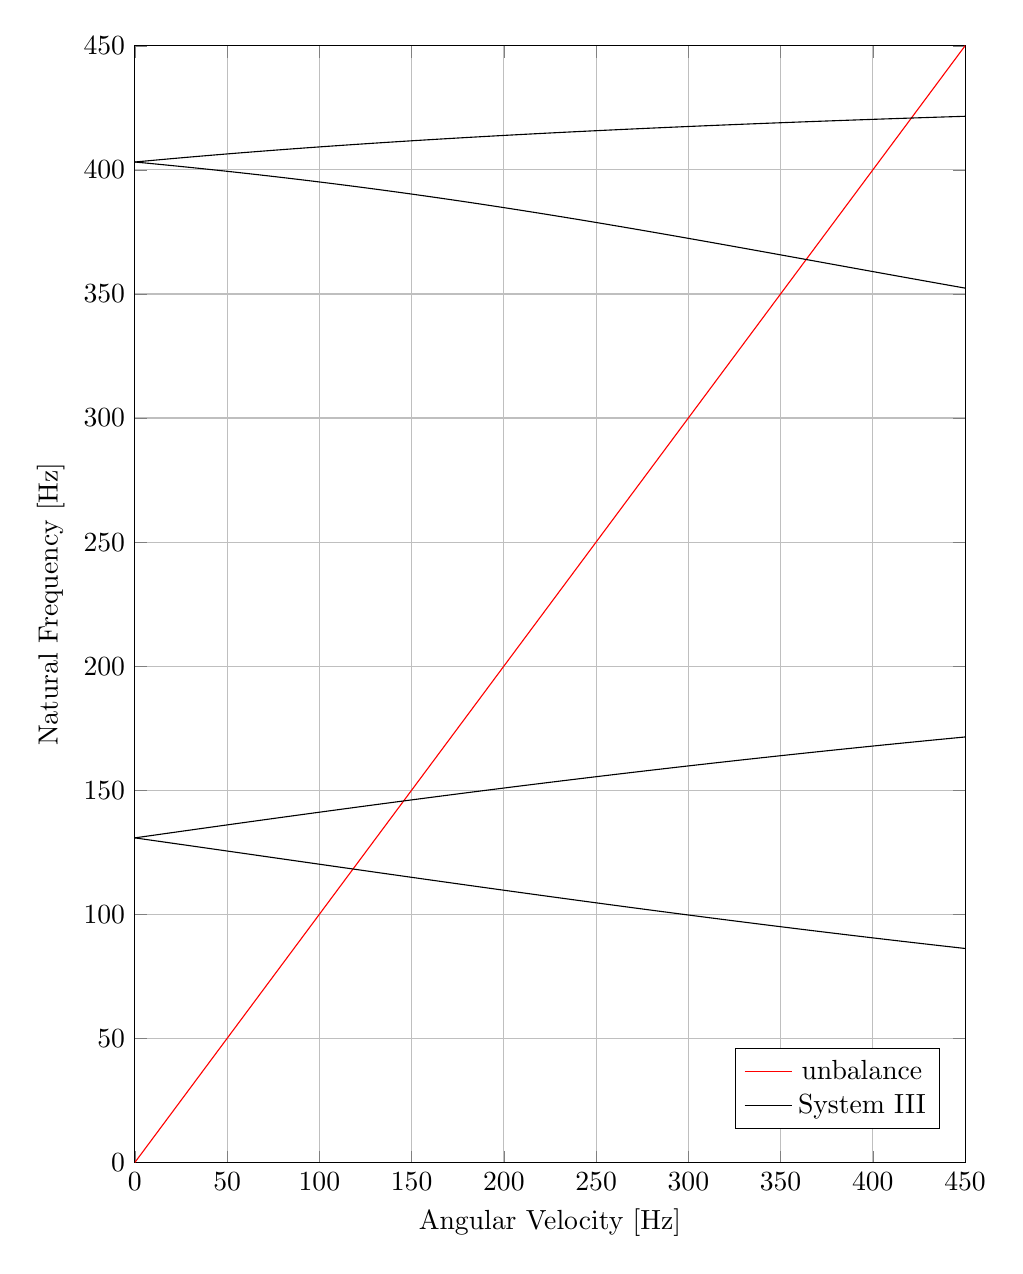
\begin{tikzpicture}
    \begin{axis}[%
    width=1\linewidth,
    height=1.3\linewidth,
    xmin=0,
    xmax=450,
    xlabel={Angular Velocity [Hz]},
    ymin=0,
    ymax=450,
    ylabel={Natural Frequency [Hz]},
    grid=major,
    legend pos = south east,
    ]
    \addplot [color=red]
      table[row sep=crcr]{%
    0	0\\
    7.5	7.5\\
    15	15\\
    22.5	22.5\\
    30	30\\
    37.5	37.5\\
    45	45\\
    52.5	52.5\\
    60	60\\
    67.5	67.5\\
    75	75\\
    82.5	82.5\\
    90	90\\
    97.5	97.5\\
    105	105\\
    112.5	112.5\\
    120	120\\
    127.5	127.5\\
    135	135\\
    142.5	142.5\\
    150	150\\
    157.5	157.5\\
    165	165\\
    172.5	172.5\\
    180	180\\
    187.5	187.5\\
    195	195\\
    202.5	202.5\\
    210	210\\
    217.5	217.5\\
    225	225\\
    232.5	232.5\\
    240	240\\
    247.5	247.5\\
    255	255\\
    262.5	262.5\\
    270	270\\
    277.5	277.5\\
    285	285\\
    292.5	292.5\\
    300	300\\
    307.5	307.5\\
    315	315\\
    322.5	322.5\\
    330	330\\
    337.5	337.5\\
    345	345\\
    352.5	352.5\\
    360	360\\
    367.5	367.5\\
    375	375\\
    382.5	382.5\\
    390	390\\
    397.5	397.5\\
    405	405\\
    412.5	412.5\\
    420	420\\
    427.5	427.5\\
    435	435\\
    442.5	442.5\\
    450	450\\
    457.5	457.5\\
    465	465\\
    472.5	472.5\\
    480	480\\
    487.5	487.5\\
    495	495\\
    502.5	502.5\\
    510	510\\
    517.5	517.5\\
    525	525\\
    532.5	532.5\\
    540	540\\
    547.5	547.5\\
    555	555\\
    562.5	562.5\\
    570	570\\
    577.5	577.5\\
    585	585\\
    592.5	592.5\\
    600	600\\
    607.5	607.5\\
    615	615\\
    622.5	622.5\\
    630	630\\
    637.5	637.5\\
    645	645\\
    652.5	652.5\\
    660	660\\
    667.5	667.5\\
    675	675\\
    682.5	682.5\\
    690	690\\
    697.5	697.5\\
    705	705\\
    712.5	712.5\\
    720	720\\
    727.5	727.5\\
    735	735\\
    742.5	742.5\\
    750	750\\
    757.5	757.5\\
    765	765\\
    772.5	772.5\\
    780	780\\
    787.5	787.5\\
    795	795\\
    802.5	802.5\\
    810	810\\
    817.5	817.5\\
    825	825\\
    832.5	832.5\\
    840	840\\
    847.5	847.5\\
    855	855\\
    862.5	862.5\\
    870	870\\
    877.5	877.5\\
    885	885\\
    892.5	892.5\\
    900	900\\
    907.5	907.5\\
    915	915\\
    922.5	922.5\\
    930	930\\
    937.5	937.5\\
    945	945\\
    952.5	952.5\\
    960	960\\
    967.5	967.5\\
    975	975\\
    982.5	982.5\\
    990	990\\
    997.5	997.5\\
    1005	1005\\
    1012.5	1012.5\\
    1020	1020\\
    1027.5	1027.5\\
    1035	1035\\
    1042.5	1042.5\\
    1050	1050\\
    1057.5	1057.5\\
    1065	1065\\
    1072.5	1072.5\\
    1080	1080\\
    1087.5	1087.5\\
    1095	1095\\
    1102.5	1102.5\\
    1110	1110\\
    1117.5	1117.5\\
    };
    \addlegendentry{unbalance}
    
    \addplot [black]
      table[row sep=crcr]{%
    0	130.803903895619\\
    7.5	130.01261155179\\
    15	129.219876509548\\
    22.5	128.425967083888\\
    30	127.630943489819\\
    37.5	126.835098381599\\
    45	126.03848042\\
    52.5	125.241574570652\\
    60	124.444057054387\\
    67.5	123.6464556624\\
    75	122.848785714771\\
    82.5	122.051306237278\\
    90	121.254166243174\\
    97.5	120.457548626825\\
    105	119.661626005079\\
    112.5	118.866529366171\\
    120	118.072449562586\\
    127.5	117.279599994112\\
    135	116.488053120412\\
    142.5	115.698092033291\\
    150	114.909799798545\\
    157.5	114.123342984866\\
    165	113.338905863959\\
    172.5	112.556620739347\\
    180	111.776677212688\\
    187.5	110.999202195297\\
    195	110.224351169728\\
    202.5	109.452246235456\\
    210	108.683041987936\\
    217.5	107.91690454177\\
    225	107.153913456389\\
    232.5	106.394246450013\\
    240	105.638026099803\\
    247.5	104.885319702469\\
    255	104.136330189039\\
    262.5	103.391099614829\\
    270	102.649776819824\\
    277.5	101.912443962138\\
    285	101.179231351348\\
    292.5	100.450216867413\\
    300	99.7254918976935\\
    307.5	99.0051426848409\\
    315	98.2892703416997\\
    322.5	97.5779534442154\\
    330	96.8712487614912\\
    337.5	96.1692440493102\\
    345	95.4719975276023\\
    352.5	94.7795833474879\\
    360	94.0920629200549\\
    367.5	93.4094740213905\\
    375	92.7318705370307\\
    382.5	92.0593219545774\\
    390	91.3918470881858\\
    397.5	90.7294915183138\\
    405	90.0722981504767\\
    412.5	89.4202973947728\\
    420	88.7735167731116\\
    427.5	88.1319774850496\\
    435	87.4956946879432\\
    442.5	86.8647104208531\\
    450	86.2390148600961\\
    457.5	85.6186371060751\\
    465	85.0035790374145\\
    472.5	84.3938411908464\\
    480	83.7894423994916\\
    487.5	83.1903744174381\\
    495	82.5966366129513\\
    502.5	82.0082218757706\\
    510	81.4251322731929\\
    517.5	80.8473437918009\\
    525	80.2748598902475\\
    532.5	79.7076644072505\\
    540	79.1457343855335\\
    547.5	78.5890605187277\\
    555	78.0376145253539\\
    562.5	77.4913905226237\\
    570	76.9503502036759\\
    577.5	76.4144777991894\\
    585	75.8837501342443\\
    592.5	75.3581332454361\\
    600	74.8375993395776\\
    607.5	74.3221244500585\\
    615	73.8116758881726\\
    622.5	73.3062214677756\\
    630	72.8057239503934\\
    637.5	72.3101512543249\\
    645	71.8194694428927\\
    652.5	71.3336470948589\\
    660	70.8526418207705\\
    667.5	70.3764192433836\\
    675	69.9049455094481\\
    682.5	69.4381701942424\\
    690	68.9760614764057\\
    697.5	68.5185873373897\\
    705	68.0656917362538\\
    712.5	67.6173451535238\\
    720	67.1735058248694\\
    727.5	66.7341317251169\\
    735	66.2991810275753\\
    742.5	65.8686135458549\\
    750	65.4423829859731\\
    757.5	65.0204531489132\\
    765	64.6027800314534\\
    772.5	64.1893199497449\\
    780	63.7800335030228\\
    787.5	63.3748748281117\\
    795	62.9738037828169\\
    802.5	62.5767786512393\\
    810	62.1837569968416\\
    817.5	61.7946960327045\\
    825	61.409553552932\\
    832.5	61.0282873525078\\
    840	60.6508599748495\\
    847.5	60.2772237910012\\
    855	59.9073410105462\\
    862.5	59.5411698986817\\
    870	59.1786663323732\\
    877.5	58.8197936236273\\
    885	58.4645101102651\\
    892.5	58.1127737008176\\
    900	57.7645478719144\\
    907.5	57.4197880309194\\
    915	57.078459904304\\
    922.5	56.7405210413445\\
    930	56.4059323951989\\
    937.5	56.0746566508458\\
    945	55.7466557898715\\
    952.5	55.4218894514376\\
    960	55.1003228678103\\
    967.5	54.7819196491237\\
    975	54.4666372556773\\
    982.5	54.1544442418124\\
    990	53.8453018141695\\
    997.5	53.5391760870518\\
    1005	53.2360323590907\\
    1012.5	52.9358302184237\\
    1020	52.6385378421288\\
    1027.5	52.3441228381217\\
    1035	52.0525481652717\\
    1042.5	51.763782051691\\
    1050	51.4777907428613\\
    1057.5	51.1945405125429\\
    1065	50.9139983416625\\
    1072.5	50.6361318296504\\
    1080	50.3609111783778\\
    1087.5	50.0883033752083\\
    1095	49.8182766308119\\
    1102.5	49.5508010531821\\
    1110	49.2858458740053\\
    1117.5	49.02338075055\\
    };
    \addlegendentry{System III}
    
    \addplot [black, forget plot]
      table[row sep=crcr]{%
    0	130.803903896033\\
    7.5	131.593757511252\\
    15	132.381841214025\\
    22.5	133.168099585939\\
    30	133.952260050874\\
    37.5	134.734300521283\\
    45	135.513934140389\\
    52.5	136.291360227898\\
    60	137.06587759837\\
    67.5	137.837749099193\\
    75	138.606646789618\\
    82.5	139.372540330538\\
    90	140.135268461166\\
    97.5	140.89471790308\\
    105	141.650768138938\\
    112.5	142.40324077929\\
    120	143.152048541384\\
    127.5	143.897145870872\\
    135	144.638280021748\\
    142.5	145.375537920101\\
    150	146.108690734732\\
    157.5	146.837649896548\\
    165	147.562368595976\\
    172.5	148.282718803641\\
    180	148.998686185732\\
    187.5	149.710148515927\\
    195	150.417052731529\\
    202.5	151.11928095871\\
    210	151.816797925876\\
    217.5	152.509605601564\\
    225	153.197530510551\\
    232.5	153.880626050119\\
    240	154.558835583595\\
    247.5	155.231989213804\\
    255	155.900249894426\\
    262.5	156.56340501819\\
    270	157.22151979201\\
    277.5	157.8745019685\\
    285	158.522408433172\\
    292.5	159.165158632513\\
    300	159.802732014947\\
    307.5	160.435104161031\\
    315	161.062313940528\\
    322.5	161.684346867158\\
    330	162.301139026861\\
    337.5	162.912736387315\\
    345	163.519108541654\\
    352.5	164.120294532046\\
    360	164.716307770551\\
    367.5	165.307094716303\\
    375	165.892670912751\\
    382.5	166.473133639132\\
    390	167.048405577469\\
    397.5	167.618520393405\\
    405	168.183529766253\\
    412.5	168.743442718713\\
    420	169.298279174943\\
    427.5	169.848042862886\\
    435	170.392728955497\\
    442.5	170.932471596099\\
    450	171.467179436317\\
    457.5	171.99696233137\\
    465	172.52181608387\\
    472.5	173.041739294702\\
    480	173.556845197705\\
    487.5	174.067118429096\\
    495	174.572601468695\\
    502.5	175.073310842174\\
    510	175.569336366019\\
    517.5	176.060621837892\\
    525	176.547295108259\\
    532.5	177.029377971693\\
    540	177.506860038579\\
    547.5	177.979831498615\\
    555	178.448270335362\\
    562.5	178.91232022433\\
    570	179.371912617824\\
    577.5	179.827143533226\\
    585	180.278076050323\\
    592.5	180.724700720356\\
    600	181.167059335685\\
    607.5	181.605239731017\\
    615	182.039269903345\\
    622.5	182.469191083679\\
    630	182.895006525897\\
    637.5	183.316776938425\\
    645	183.734546279258\\
    652.5	184.14839806846\\
    660	184.558328434873\\
    667.5	184.964390850437\\
    675	185.366659956984\\
    682.5	185.765114203765\\
    690	186.159803278661\\
    697.5	186.550838347164\\
    705	186.938191232102\\
    712.5	187.321915904463\\
    720	187.70207722367\\
    727.5	188.078703796534\\
    735	188.451829426034\\
    742.5	188.821509615794\\
    750	189.187744229824\\
    757.5	189.550623599345\\
    765	189.91017383109\\
    772.5	190.266412754476\\
    780	190.619407375033\\
    787.5	190.969156393699\\
    795	191.315728217422\\
    802.5	191.659153395184\\
    810	191.999480824137\\
    817.5	192.336730093168\\
    825	192.670939246855\\
    832.5	193.002136070787\\
    840	193.330421601824\\
    847.5	193.655738788288\\
    855	193.978182286912\\
    862.5	194.297776309777\\
    870	194.614504718139\\
    877.5	194.928468411766\\
    885	195.239684769964\\
    892.5	195.548152489004\\
    900	195.853973080147\\
    907.5	196.15708750315\\
    915	196.457624276936\\
    922.5	196.755558015901\\
    930	197.050912501566\\
    937.5	197.343749098068\\
    945	197.63410039125\\
    952.5	197.921953081407\\
    960	198.20737148185\\
    967.5	198.490393393636\\
    975	198.771046713099\\
    982.5	199.049342011349\\
    990	199.325292550877\\
    997.5	199.598973516352\\
    1005	199.870388177519\\
    1012.5	200.139572967499\\
    1020	200.406506225015\\
    1027.5	200.671294093052\\
    1035	200.933895451054\\
    1042.5	201.194387629136\\
    1050	201.452780106508\\
    1057.5	201.709071879636\\
    1065	201.963320064031\\
    1072.5	202.215508094109\\
    1080	202.46572648112\\
    1087.5	202.713958368449\\
    1095	202.960211216472\\
    1102.5	203.204534475252\\
    1110	203.446940940084\\
    1117.5	203.687457756117\\
    };
    \addplot [black, forget plot]
      table[row sep=crcr]{%
    0	403.171424503726\\
    7.5	402.642907562951\\
    15	402.102390667794\\
    22.5	401.550864341336\\
    30	400.987438198565\\
    37.5	400.412329939315\\
    45	399.824994368896\\
    52.5	399.225304935395\\
    60	398.613386654043\\
    67.5	397.988650239755\\
    75	397.351270373986\\
    82.5	396.700940300041\\
    90	396.037608832101\\
    97.5	395.361047085577\\
    105	394.671211451821\\
    112.5	393.968228837457\\
    120	393.25195394217\\
    127.5	392.522207698752\\
    135	391.779277640947\\
    142.5	391.022732244437\\
    150	390.253017100706\\
    157.5	389.470163176631\\
    165	388.674167817308\\
    172.5	387.865299281792\\
    180	387.043510687054\\
    187.5	386.209116568227\\
    195	385.362311562059\\
    202.5	384.503504472612\\
    210	383.632900045058\\
    217.5	382.750626016685\\
    225	381.857367857781\\
    232.5	380.953197050371\\
    240	380.03861394151\\
    247.5	379.114273414109\\
    255	378.180202522293\\
    262.5	377.237278395818\\
    270	376.285746411417\\
    277.5	375.326293489552\\
    285	374.359343502581\\
    292.5	373.385475314897\\
    300	372.405306178588\\
    307.5	371.419418868607\\
    315	370.428305910114\\
    322.5	369.432563931041\\
    330	368.432886807505\\
    337.5	367.42977698353\\
    345	366.423884392479\\
    352.5	365.415704821423\\
    360	364.405877355356\\
    367.5	363.395008473056\\
    375	362.383677405615\\
    382.5	361.372277656293\\
    390	360.361519904291\\
    397.5	359.351889924345\\
    405	358.343845437912\\
    412.5	357.337896401967\\
    420	356.334516435551\\
    427.5	355.334192380519\\
    435	354.337401924384\\
    442.5	353.3444109226\\
    450	352.355774155416\\
    457.5	351.371775923287\\
    465	350.392809827197\\
    472.5	349.41923831496\\
    480	348.451308625531\\
    487.5	347.489359844256\\
    495	346.533664668506\\
    502.5	345.584493359899\\
    510	344.642049496191\\
    517.5	343.7066144388\\
    525	342.778333802886\\
    532.5	341.857404775062\\
    540	340.944068886422\\
    547.5	340.038319020568\\
    555	339.140455859443\\
    562.5	338.250548380841\\
    570	337.368633281539\\
    577.5	336.494902699046\\
    585	335.629390460724\\
    592.5	334.772185656279\\
    600	333.923344861416\\
    607.5	333.082898458274\\
    615	332.25088904708\\
    622.5	331.427343330674\\
    630	330.612288783535\\
    637.5	329.80572804633\\
    645	329.007658595898\\
    652.5	328.218065832352\\
    660	327.436951306424\\
    667.5	326.664274825126\\
    675	325.90001755248\\
    682.5	325.144150429266\\
    690	324.396632987894\\
    697.5	323.657415363744\\
    705	322.926453347546\\
    712.5	322.203679361179\\
    720	321.48908013958\\
    727.5	320.782549168258\\
    735	320.084043863324\\
    742.5	319.393493141206\\
    750	318.710826486422\\
    757.5	318.035976575434\\
    765	317.368868643036\\
    772.5	316.709426295291\\
    780	316.057574365099\\
    787.5	315.413229955792\\
    795	314.776318258042\\
    802.5	314.146747315751\\
    810	313.524449643796\\
    817.5	312.909336266134\\
    825	312.301319636006\\
    832.5	311.700319497637\\
    840	311.106256304997\\
    847.5	310.519035877564\\
    855	309.938578467111\\
    862.5	309.36480173304\\
    870	308.797606694302\\
    877.5	308.236924341533\\
    885	307.682666927399\\
    892.5	307.134740048625\\
    900	306.59307957454\\
    907.5	306.05757561362\\
    915	305.528172866011\\
    922.5	305.004772602673\\
    930	304.4872903271\\
    937.5	303.975655197987\\
    945	303.469787799896\\
    952.5	302.969596771662\\
    960	302.474972732598\\
    967.5	301.98589913138\\
    975	301.502278207459\\
    982.5	301.024021751813\\
    990	300.551048876337\\
    997.5	300.083301932922\\
    1005	299.620695812416\\
    1012.5	299.163166451552\\
    1020	298.710615776433\\
    1027.5	298.263006000188\\
    1035	297.820239330497\\
    1042.5	297.38226989062\\
    1050	296.949006068385\\
    1057.5	296.520387013755\\
    1065	296.096354223575\\
    1072.5	295.676821645798\\
    1080	295.261755244355\\
    1087.5	294.851066665591\\
    1095	294.444692362741\\
    1102.5	294.042575191812\\
    1110	293.644651423361\\
    1117.5	293.250864424344\\
    };
    \addplot [black, forget plot]
      table[row sep=crcr]{%
    0	403.171424504001\\
    7.5	403.689566759961\\
    15	404.196161895155\\
    22.5	404.692604966684\\
    30	405.178455604435\\
    37.5	405.654338352331\\
    45	406.120149451482\\
    52.5	406.576193566943\\
    60	407.022946591543\\
    67.5	407.460226308726\\
    75	407.888571516853\\
    82.5	408.308048364639\\
    90	408.71893362829\\
    97.5	409.121304121322\\
    105	409.515421239113\\
    112.5	409.901703261391\\
    120	410.280246740331\\
    127.5	410.651077564859\\
    135	411.014736518362\\
    142.5	411.370858001228\\
    150	411.720095428681\\
    157.5	412.06257436296\\
    165	412.398353729929\\
    172.5	412.727763427836\\
    180	413.050711911938\\
    187.5	413.367505704876\\
    195	413.678279188036\\
    202.5	413.983364329149\\
    210	414.282820401396\\
    217.5	414.576547766233\\
    225	414.865134701712\\
    232.5	415.148314514284\\
    240	415.426341548862\\
    247.5	415.699681049824\\
    255	415.967856991726\\
    262.5	416.231554449255\\
    270	416.490538862676\\
    277.5	416.745187630151\\
    285	416.995321766098\\
    292.5	417.241267716797\\
    300	417.483149494096\\
    307.5	417.721083051071\\
    315	417.955014526804\\
    322.5	418.185053201474\\
    330	418.411491938937\\
    337.5	418.63424862506\\
    345	418.853556295715\\
    352.5	419.069314734378\\
    360	419.281683569556\\
    367.5	419.490849596096\\
    375	419.696918199891\\
    382.5	419.89966033124\\
    390	420.099479474897\\
    397.5	420.296388144237\\
    405	420.49033334468\\
    412.5	420.681433168792\\
    420	420.869756492682\\
    427.5	421.055430908137\\
    435	421.238620210059\\
    442.5	421.419035680806\\
    450	421.59710710931\\
    457.5	421.772657169368\\
    465	421.945847184797\\
    472.5	422.116820926307\\
    480	422.285391326425\\
    487.5	422.451760058629\\
    495	422.61595748331\\
    502.5	422.778082875167\\
    510	422.938040833892\\
    517.5	423.096119536092\\
    525	423.25212719378\\
    532.5	423.406159824465\\
    540	423.558450210138\\
    547.5	423.708696365814\\
    555	423.857317193533\\
    562.5	424.004076236761\\
    570	424.149092696001\\
    577.5	424.292456374382\\
    585	424.434105590872\\
    592.5	424.574178986049\\
    600	424.712724202946\\
    607.5	424.849649516186\\
    615	424.985072153744\\
    622.5	425.118894029581\\
    630	425.251367701576\\
    637.5	425.38246359441\\
    645	425.512162197953\\
    652.5	425.640397449287\\
    660	425.767348051013\\
    667.5	425.892987429851\\
    675	426.017263337855\\
    682.5	426.140341078691\\
    690	426.262249707801\\
    697.5	426.382844823307\\
    705	426.502283502697\\
    712.5	426.620577015049\\
    720	426.737737256468\\
    727.5	426.853753433165\\
    735	426.968688915914\\
    742.5	427.082521359826\\
    750	427.195365580306\\
    757.5	427.307134182525\\
    765	427.417845651502\\
    772.5	427.527599485487\\
    780	427.636343934725\\
    787.5	427.744182157186\\
    795	427.851057655694\\
    802.5	427.957030914287\\
    810	428.062059442133\\
    817.5	428.166257252255\\
    825	428.269497619846\\
    832.5	428.371934014355\\
    840	428.473468464286\\
    847.5	428.574222252339\\
    855	428.674142741146\\
    862.5	428.773242679933\\
    870	428.871622008984\\
    877.5	428.969189215019\\
    885	429.066072068841\\
    892.5	429.162174931895\\
    900	429.257473399378\\
    907.5	429.352171421413\\
    915	429.446054391539\\
    922.5	429.539273739104\\
    930	429.631850720097\\
    937.5	429.723734255995\\
    945	429.814931208086\\
    952.5	429.905550151536\\
    960	429.995476774025\\
    967.5	430.084782936705\\
    975	430.173446822492\\
    982.5	430.261520466128\\
    990	430.349049416027\\
    997.5	430.435937666652\\
    1005	430.522261199865\\
    1012.5	430.607974797903\\
    1020	430.693225434997\\
    1027.5	430.777841314839\\
    1035	430.861980961993\\
    1042.5	430.945539000039\\
    1050	431.028545892679\\
    1057.5	431.11109604214\\
    1065	431.193100665207\\
    1072.5	431.274672449339\\
    1080	431.355674031882\\
    1087.5	431.436194321209\\
    1095	431.516284918537\\
    1102.5	431.595891920893\\
    1110	431.675043471667\\
    1117.5	431.753745981281\\
    };
    \end{axis}
\end{tikzpicture}%    
    \caption{}
    \label{fig:unbalance_response_natural}
\end{subfigure}
\hfill
\begin{subfigure}[t]{0.49\textwidth}
    \centering
    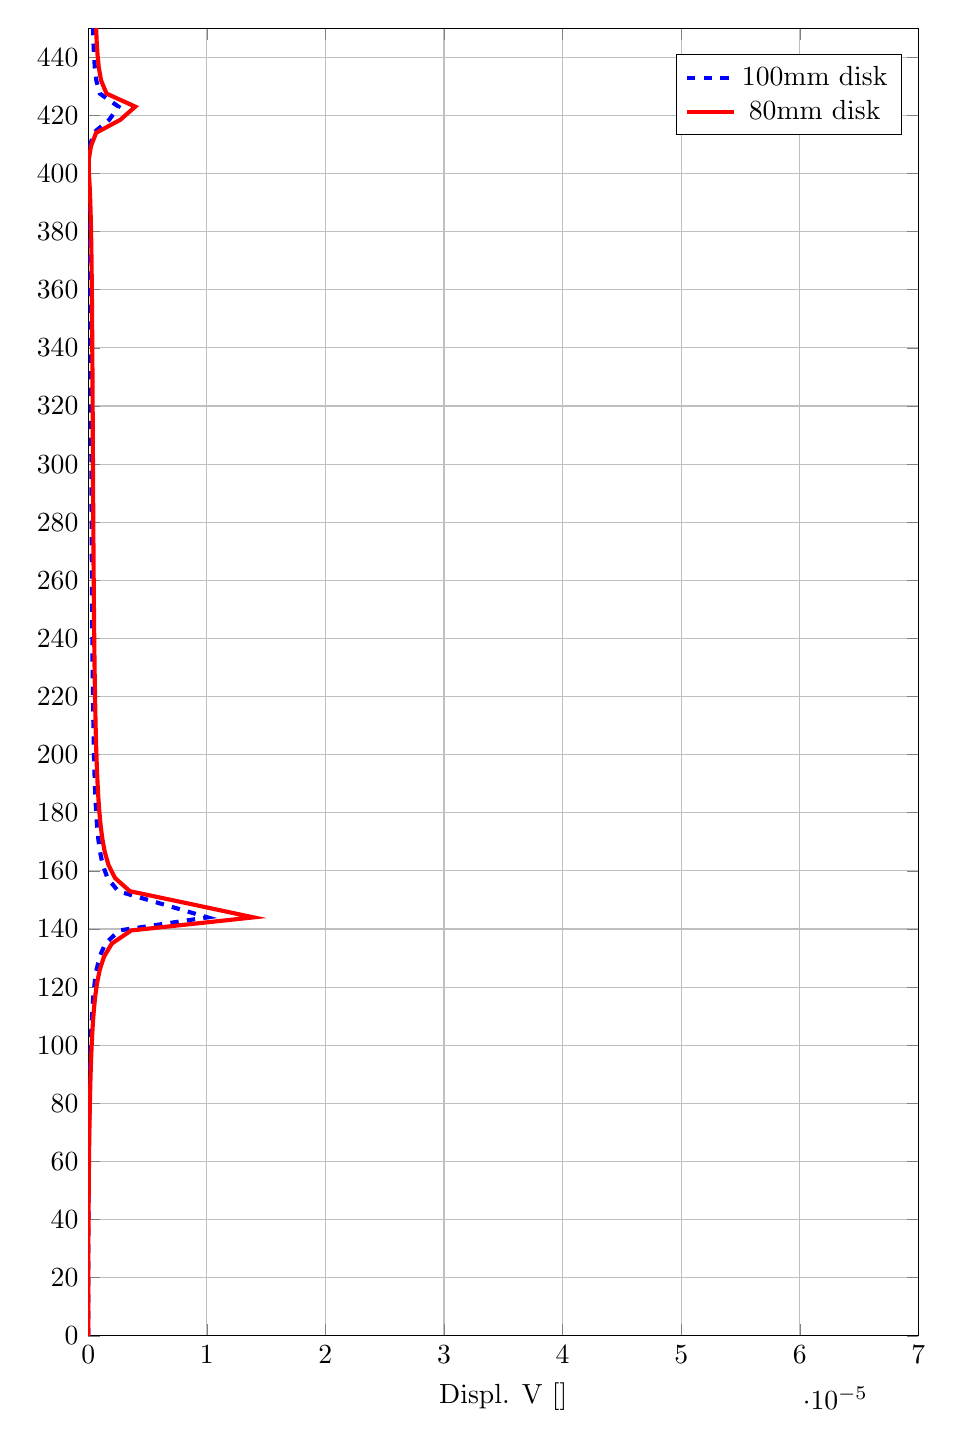
\begin{tikzpicture}

\begin{axis}[%
    width=1\linewidth,
    height=1.5\linewidth,
    xmin=0,
    xmax=7e-05,
    xlabel={Displ. V [\si{\meter}]},
    ymin=0,
    ymax=450,
    grid=major,
    ]
    \addplot [color=blue, dashed, line width=1.5pt]
      table[row sep=crcr]{%
    0	0\\
    2.33536039825968e-10	4.5\\
    9.36748387821509e-10	9\\
    2.11752485625866e-09	13.5\\
    3.78926629671696e-09	18\\
    5.97128296915819e-09	22.5\\
    8.68938004066146e-09	27\\
    1.19766660961999e-08	31.5\\
    1.5874633435508e-08	36\\
    2.04345787002309e-08	40.5\\
    2.57194594146702e-08	45\\
    3.18063198977937e-08	49.5\\
    3.87894741607144e-08	54\\
    4.67847123516737e-08	58.5\\
    5.59349146211689e-08	63\\
    6.64176341060982e-08	67.5\\
    7.84554860770015e-08	72\\
    9.23306166392138e-08	76.5\\
    1.08405233756433e-07	81\\
    1.27151369947678e-07	85.5\\
    1.49195095441845e-07	90\\
    1.75384071425718e-07	94.5\\
    2.06894188127415e-07	99\\
    2.45404468376152e-07	103.5\\
    2.93397291634169e-07	108\\
    3.54702883802163e-07	112.5\\
    4.35556282473915e-07	117\\
    5.46834181354803e-07	121.5\\
    7.09359445211531e-07	126\\
    9.68635813268812e-07	130.5\\
    1.44680668721819e-06	135\\
    2.62133842813075e-06	139.5\\
    1.00622914488689e-05	144\\
    6.31032319668101e-06	148.5\\
    2.53212470219972e-06	153\\
    1.63281644993207e-06	157.5\\
    1.2298126574528e-06	162\\
    1.00115570815366e-06	166.5\\
    8.53837128411111e-07	171\\
    7.51004947460305e-07	175.5\\
    6.75139553557536e-07	180\\
    6.16846431055669e-07	184.5\\
    5.70635262752876e-07	189\\
    5.33082602517155e-07	193.5\\
    5.01942845875901e-07	198\\
    4.75681707790006e-07	202.5\\
    4.53215138609939e-07	207\\
    4.33755347966474e-07	211.5\\
    4.16715951443639e-07	216\\
    4.01651345425739e-07	220.5\\
    3.88216715067878e-07	225\\
    3.7614091973257e-07	229.5\\
    3.65207661582446e-07	234\\
    3.55242124897147e-07	238.5\\
    3.46101313891985e-07	243\\
    3.37666943194839e-07	247.5\\
    3.29840122845495e-07	252\\
    3.22537325603195e-07	256.5\\
    3.15687283814822e-07	261\\
    3.09228568543276e-07	265.5\\
    3.03107674598101e-07	270\\
    2.97277483594518e-07	274.5\\
    2.9169601066071e-07	279\\
    2.86325363806904e-07	283.5\\
    2.81130861305685e-07	288\\
    2.7608026377792e-07	292.5\\
    2.71143085332884e-07	297\\
    2.66289952911219e-07	301.5\\
    2.61491985363007e-07	306\\
    2.5672016400964e-07	310.5\\
    2.51944664325998e-07	315\\
    2.47134113634286e-07	319.5\\
    2.42254731512338e-07	324\\
    2.37269296734899e-07	328.5\\
    2.32135864816597e-07	333\\
    2.26806130179444e-07	337.5\\
    2.21223280880736e-07	342\\
    2.15319122195282e-07	346.5\\
    2.09010131763621e-07	351\\
    2.02191924751747e-07	355.5\\
    1.94731300378737e-07	360\\
    1.86454513239284e-07	364.5\\
    1.77129472716116e-07	369\\
    1.66437830020524e-07	373.5\\
    1.53929521983272e-07	378\\
    1.38945373499466e-07	382.5\\
    1.20478067745203e-07	387\\
    9.69054277248407e-08	391.5\\
    6.54344196919938e-08	396\\
    2.0809020093935e-08	400.5\\
    4.8177173880853e-08	405\\
    1.70433681828533e-07	409.5\\
    4.5036800428842e-07	414\\
    1.77804017465607e-06	418.5\\
    2.5566997938065e-06	423\\
    9.85673558704698e-07	427.5\\
    6.86441060170491e-07	432\\
    5.58992158420021e-07	436.5\\
    4.88008639899028e-07	441\\
    4.42523291071426e-07	445.5\\
    4.10717975279491e-07	450\\
    };
    \addlegendentry{100mm disk}
    
    \addplot [color=red, line width=1.5pt]
      table[row sep=crcr]{%
    0	0\\
    3.15432249694727e-10	4.5\\
    1.26534132366486e-09	9\\
    2.86066830932807e-09	13.5\\
    5.12000104282192e-09	18\\
    8.07012340917477e-09	22.5\\
    1.17468267448046e-08	27\\
    1.61960302983985e-08	31.5\\
    2.14752783438853e-08	36\\
    2.76557089377233e-08	40.5\\
    3.48246267849306e-08	45\\
    4.30888651665247e-08	49.5\\
    5.25791969339253e-08	54\\
    6.34561639857961e-08	58.5\\
    7.59178572177679e-08	63\\
    9.02104253760791e-08	67.5\\
    1.0664247283341e-07	72\\
    1.2560511101647e-07	76.5\\
    1.4760041130616e-07	81\\
    1.73282651656763e-07	85.5\\
    2.0351958938806e-07	90\\
    2.394860798549e-07	94.5\\
    2.82811860848787e-07	99\\
    3.35823942729316e-07	103.5\\
    4.01962673963067e-07	108\\
    4.86536322439652e-07	112.5\\
    5.98185870994343e-07	117\\
    7.51984948700691e-07	121.5\\
    9.76791093951483e-07	126\\
    1.33566584595368e-06	130.5\\
    1.99788184078149e-06	135\\
    3.62513610998094e-06	139.5\\
    1.39366980989634e-05	144\\
    8.75379022761634e-06	148.5\\
    3.51828340274934e-06	153\\
    2.27249989666743e-06	157.5\\
    1.71453254021573e-06	162\\
    1.39819608043998e-06	166.5\\
    1.19459446815842e-06	171\\
    1.05265614530469e-06	175.5\\
    9.48101297889061e-07	180\\
    8.67910268030985e-07	184.5\\
    8.04474021509156e-07	189\\
    7.53047886519535e-07	193.5\\
    7.10519491233627e-07	198\\
    6.74762232885551e-07	202.5\\
    6.44273453257708e-07	207\\
    6.17961049546227e-07	211.5\\
    5.95012020352866e-07	216\\
    5.74808446571271e-07	220.5\\
    5.568720664319e-07	225\\
    5.40826696481742e-07	229.5\\
    5.26372131422894e-07	234\\
    5.13265625140954e-07	238.5\\
    5.01308496813792e-07	243\\
    4.90336274046557e-07	247.5\\
    4.80211322261852e-07	252\\
    4.70817250364241e-07	256.5\\
    4.62054603662179e-07	261\\
    4.53837501130258e-07	265.5\\
    4.4609097236363e-07	270\\
    4.38748816704315e-07	274.5\\
    4.31751853365164e-07	279\\
    4.25046463692692e-07	283.5\\
    4.18583349222457e-07	288\\
    4.1231644472928e-07	292.5\\
    4.06201935859213e-07	297\\
    4.0019733727127e-07	301.5\\
    3.9426059011863e-07	306\\
    3.88349137427707e-07	310.5\\
    3.82418932236296e-07	315\\
    3.76423325683572e-07	319.5\\
    3.7031176935983e-07	324\\
    3.64028246144591e-07	328.5\\
    3.57509313158008e-07	333\\
    3.50681593993103e-07	337.5\\
    3.4345848624756e-07	342\\
    3.35735739840896e-07	346.5\\
    3.27385386414563e-07	351\\
    3.18247216003274e-07	355.5\\
    3.08116523649622e-07	360\\
    2.96726034705456e-07	364.5\\
    2.83718468136632e-07	369\\
    2.68603508736517e-07	373.5\\
    2.50687732123789e-07	378\\
    2.28955285014766e-07	382.5\\
    2.01853546181357e-07	387\\
    1.66881928608342e-07	391.5\\
    1.1973469942847e-07	396\\
    5.23088935271285e-08	400.5\\
    5.26722130520064e-08	405\\
    2.39778366437882e-07	409.5\\
    6.69975020041552e-07	414\\
    2.71547284562442e-06	418.5\\
    3.96880663712846e-06	423\\
    1.54813397188613e-06	427.5\\
    1.08819632779155e-06	432\\
    8.9310164587941e-07	436.5\\
    7.85063278751982e-07	441\\
    7.16339009837819e-07	445.5\\
    6.68708860088106e-07	450\\
    };
    \addlegendentry{80mm disk}
    
    \end{axis}
    
    \end{tikzpicture}%
    \caption{}
    \label{fig:unbalance_response_disp}
\end{subfigure}
\caption{Unbalance response of system (III), (\subref{fig:unbalance_response_natural}) shows the natural frequencies and (\subref{fig:unbalance_response_disp}) shows the displacement}
\label{fig:unbalance_response}
\end{figure}
From figure \ref{fig:unbalance_response} it looks like the response is below the maximum. However, as there is no damping in the system,
the response will increase to infinity at the critical speed. As such, the maximum displacement is a function of how many steps, or how precise this infinity can be calculated.
Therefore it's not possible to determine wheter the response is below the maximum, as the maximum is always infinity even at very low unbalance.

\section{Modelling of Hydrodynamic Bearing}
Instead of using ball bearings, the use of hydrodynamic bearings is considered. The ball bearing positioned at \textcolor{red}{B1} in figure \ref{fig:shaft_geometry} is replaced with a two-axial-groove bearing for system  system (III)

\subsection{Hydrodynamic bearing - Properties}
First the properties of the specific hydrodynamic bearing is found.

\subsubsection{Assumptions}
The fluid inside the hydrodynamic bearing is assumed to be incompressible and the flow is assumed to be laminar. The bearing is assumed to be perfectly balanced.

\subsubsection{External static load}
To calculate the external static load a free body diagram is made. The free body diagram is shown in figure \ref{fig:free_body_diagram}.
\begin{figure}[ht]
    \centering
    %\begin{tikzpicture}[scale=\textwidth/1cm]
%
%    \draw[fill=gray!10] (0,0) -- (1,0) -- (1,0.01) -- (0,0.01) -- cycle;    % shaft
%
%    \draw[force] (0.3, -0.05)node[below]{$F_{R1}$} -- (0.3, 0);    % reaction force
%    \draw[force] (0.9, -0.05)node[below]{$F_{R2}$} -- (0.9, 0);    % reaction force
%
%    \draw[force] (0.5, 0.06)node[above]{$F_{S}$} -- (0.5, 0.01);    % Shaft gravity force
%    \draw[force] (0.05, 0.06)node[above]{$F_{D1}$} -- (0.05, 0.01);    % Disk 1 gravity force
%    \draw[force] (0.15, 0.06)node[above]{$F_{D2}$} -- (0.15, 0.01);    % Disk 2 gravity force
%
%    \draw[dim] (0, 0.11) -- (0.05, 0.11)node[midway, above]{$L_{D1}$};    % Disk 1 length
%    \draw[dim] (0, 0.11) -- (0.15, 0.11)node[midway, above]{$L_{D2}$};    % Disk 2 length
%    \draw[dim] (0, 0.11) -- (0.5, 0.11)node[midway, above]{$L_S$};    % Shaft length
%
%    \draw[dim] (0, -0.1) -- (0.3, -0.1)node[midway, below]{$L_{R1}$};    % Reaction 1 length
%    \draw[dim] (0, -0.1) -- (0.9, -0.1)node[midway, below]{$L_{R2}$};    % Reaction 2 length
%
%\end{tikzpicture}

\begin{tikzpicture}[scale=\linewidth/120cm]

    % Bearing mounts
    %\draw[red, dashed] (109.75, -7) -- (109.75, 7) node[above] {B1};
    %\draw[red, dashed] (35.5, -7) -- (35.5, 7) node[above] {B2};

    \draw[force] (109.75, -7.8225)node[right]{$F_{R2}$} -- (109.75, -2.8225);    % reaction force
    \draw[force] (35.5, -9.985)node[right]{$F_{R1}$} -- (35.5, -4.985);    % reaction force

    \draw[force] (57.5, 9.485)node[right]{$F_{S}$} -- (57.5, 4.485);    % Shaft gravity force

    % Discs
    %\draw[blue, dashed] (19, -7) -- (19, 7) node[above] {D100};
    %\draw[blue, dashed] (10, -7) -- (10, 7) node[above] {D80};
    
    \draw[force] (12.3, 8.5)node[left]{$F_{D1}$} -- (12.3, 3.5);    % Disk 1 gravity force
    \draw[force] (18.2, 8.5)node[right]{$F_{D2}$} -- (18.2, 3.5);    % Disk 2 gravity force

    % shaft
    \draw[fill=gray!10] (0,-2.975) -- (6.5,-2.975) -- (6.5,-3.5) -- (24.0, -3.5) -- (24.0, -4.485) -- (29.5, -4.485) -- (29.5, -4.985) -- (41.5, -4.985) -- (41.5, -4.485) -- (104.0, -4.485) -- (104.0, -2.8225) -- (115.0, -2.8225) -- (115.0, 2.8225) -- (104.0, 2.8225) -- (104.0, 4.485) -- (41.5, 4.485) -- (41.5, 4.985) -- (29.5, 4.985) -- (29.5, 4.485) -- (24.0, 4.485) -- (24.0, 3.5) -- (6.5, 3.5) -- (6.5, 2.975) -- (0, 2.975) -- cycle;

    \draw[dim] (0, 13) -- (12.3, 13)node[midway, above]{$L_{D1}$};    % Disk 1 length
    \draw[dim] (0, 13) -- (18.2, 13)node[above]{$L_{D2}$};    % Disk 2 length
    \draw[dim] (0, 13) -- (57.5, 13)node[midway, above]{$L_S$};    % Shaft length

    \draw[dim] (0, -13) -- (35.5, -13)node[midway, below]{$L_{R1}$};    % Reaction 1 length
    \draw[dim] (0, -13) -- (109.5, -13)node[midway, below]{$L_{R2}$};    % Reaction 2 length


\end{tikzpicture}
    \caption{Free body diagram of hydrodynamic bearing}
    \label{fig:free_body_diagram}
\end{figure}
With the geometry given the length can be found in table \ref{tab:hydrodynamic_bearing_properties}.
\begin{table}[ht]
    \centering
    \caption{Properties of Hydrodynamic Bearing}
    \label{tab:hydrodynamic_bearing_properties}
    \begin{tabular}{@{}ccccc@{}}
        \toprule
        $L_{D1}$    &   $L_{D2}$    &   $L_S$   &   $L_{R1}$   &   $L_{R2}$   \\ \midrule
        \SI{0.123}{\meter}  &   \SI{0.182}{\meter}  &   \SI{0.575}{\meter}   &   \SI{0.355}{\meter}   &   \SI{1.095}{\meter}   \\ \bottomrule
    \end{tabular}
\end{table}
The forces are found form the greavitational force and there respective weight. The forces are shown in table \ref{tab:hydrodynamic_bearing_forces}.
\begin{table}[ht]
    \centering
    \caption{Forces in Hydrodynamic Bearing}
    \label{tab:hydrodynamic_bearing_forces}
    \begin{tabular}{@{}ccc@{}}
        \toprule
        $F_{D1}$    &   $F_{D2}$    &   $F_S$   \\ \midrule
        \SI{347.6}{\newton}  &   \SI{445.0}{\newton}  &   \SI{206.2}{\newton}   \\ \bottomrule
    \end{tabular}
\end{table}
Force equilibirum can then be used to find the reaction forces:
\begin{equation}
    R_1 + R_2 - F_{D1} - F_{D2} - F_S = 0
    \label{eq:vertical_equilibrium}
\end{equation}
\begin{equation}
    -F_{D1} L_{D1} - F_{D2} L_{D2} - F_S L_S + R_1 L_{R1} + R_2 L_{R2} = 0
    \label{eq:moment_equilibrium}
\end{equation}
Solving equation \ref{eq:vertical_equilibrium} and \ref{eq:moment_equilibrium} for $R_1$ and $R_2$ gives the reaction forces shown in table \ref{tab:hydrodynamic_bearing_reactions}.
\begin{table}[ht]
    \centering
    \caption{Reaction Forces in Hydrodynamic Bearing}
    \label{tab:hydrodynamic_bearing_reactions}
    \begin{tabular}{@{}cc@{}}
        \toprule
        $F_{R1}$    &   $F_{R2}$    \\ \midrule
        \SI{1150.7}{\newton}  &   \SI{-151.9}{\newton}  \\ \bottomrule
    \end{tabular}
\end{table}
Thus the force on the hydrodynamic bearing is \SI{1150.7}{\newton}.

\subsubsection{Oil film thickness}
The oil thickness is calculated with the bearing dimensions, the force on the bearing and the table data from \cite[Table 1a]{Problem}. The oil flim thickness is shown in figure \ref{fig:oil_film_thickness}.
\begin{figure}[ht]
    \centering
    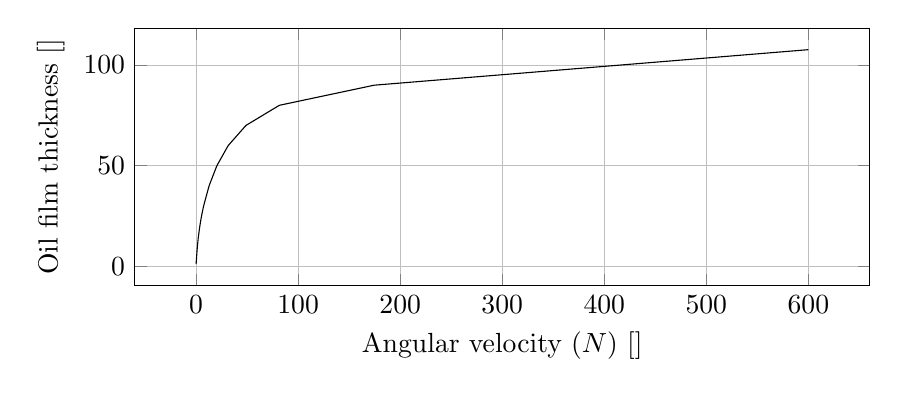
\begin{tikzpicture}

\begin{axis}[%
width=0.9\linewidth,
height=0.4\linewidth,
xlabel={Angular velocity ($N$) [\si{\hertz}]},
ylabel={Oil film thickness [\si{\micro\meter}]},
grid = major,
]
\addplot []
  table[row sep=crcr]{%
0	1.08826857789514\\
1.0016694490818	8.28216307638261\\
2.00333889816361	13.6247262499327\\
3.00500834724541	17.6284966950525\\
4.00667779632721	21.0745373053398\\
5.00834724540902	24.0731244618634\\
6.01001669449082	26.6892417811464\\
7.01168614357262	29.1342436164656\\
8.01335559265442	31.207658286659\\
9.01502504173623	33.0773655724914\\
10.016694490818	34.9470728583238\\
11.0183639398998	36.8167801441562\\
12.0200333889816	38.6864874299886\\
13.0217028380634	40.3899096976889\\
14.0233722871452	41.7006323310559\\
15.025041736227	43.011354964423\\
16.0267111853088	44.32207759779\\
17.0283806343907	45.632800231157\\
18.0300500834725	46.9435228645241\\
19.0317195325543	48.2542454978911\\
20.0333889816361	49.5649681312581\\
21.0350584307179	50.6045694246878\\
22.0367278797997	51.5094811359804\\
23.0383973288815	52.4143928472729\\
24.0400667779633	53.3193045585655\\
25.0417362270451	54.224216269858\\
26.0434056761269	55.1291279811505\\
27.0450751252087	56.0340396924431\\
28.0467445742905	56.9389514037356\\
29.0484140233723	57.8438631150281\\
30.0500834724541	58.7487748263207\\
31.0517529215359	59.6536865376132\\
32.0534223706177	60.3551269410464\\
33.0550918196995	60.9304214905333\\
34.0567612687813	61.5057160400202\\
35.0584307178631	62.0810105895071\\
36.0601001669449	62.656305138994\\
37.0617696160267	63.2315996884809\\
38.0634390651085	63.8068942379678\\
39.0651085141903	64.3821887874546\\
40.0667779632721	64.9574833369415\\
41.0684474123539	65.5327778864284\\
42.0701168614357	66.1080724359153\\
43.0717863105175	66.6833669854022\\
44.0734557595993	67.2586615348891\\
45.0751252086811	67.833956084376\\
46.0767946577629	68.4092506338628\\
47.0784641068447	68.9845451833497\\
48.0801335559265	69.5598397328366\\
49.0818030050083	70.071963075647\\
50.0834724540901	70.3783247513978\\
51.085141903172	70.6846864271487\\
52.0868113522538	70.9910481028995\\
53.0884808013356	71.2974097786504\\
54.0901502504174	71.6037714544012\\
55.0918196994992	71.9101331301521\\
56.093489148581	72.2164948059029\\
57.0951585976628	72.5228564816538\\
58.0968280467446	72.8292181574046\\
59.0984974958264	73.1355798331555\\
60.1001669449082	73.4419415089063\\
61.10183639399	73.7483031846571\\
62.1035058430718	74.054664860408\\
63.1051752921536	74.3610265361588\\
64.1068447412354	74.6673882119097\\
65.1085141903172	74.9737498876606\\
66.110183639399	75.2801115634114\\
67.1118530884808	75.5864732391622\\
68.1135225375626	75.8928349149131\\
69.1151919866444	76.1991965906639\\
70.1168614357262	76.5055582664148\\
71.118530884808	76.8119199421656\\
72.1202003338898	77.1182816179165\\
73.1218697829716	77.4246432936673\\
74.1235392320534	77.7310049694182\\
75.1252086811352	78.037366645169\\
76.126878130217	78.3437283209199\\
77.1285475792988	78.6500899966707\\
78.1302170283806	78.9564516724216\\
79.1318864774624	79.2628133481724\\
80.1335559265442	79.5691750239233\\
81.135225375626	79.8755366996741\\
82.1368948247079	80.06397273373\\
83.1385642737897	80.1717185773203\\
84.1402337228715	80.2794644209106\\
85.1419031719533	80.387210264501\\
86.1435726210351	80.4949561080913\\
87.1452420701169	80.6027019516817\\
88.1469115191987	80.710447795272\\
89.1485809682805	80.8181936388624\\
90.1502504173623	80.9259394824527\\
91.1519198664441	81.033685326043\\
92.1535893155259	81.1414311696334\\
93.1552587646077	81.2491770132237\\
94.1569282136895	81.3569228568141\\
95.1585976627713	81.4646687004044\\
96.1602671118531	81.5724145439947\\
97.1619365609349	81.6801603875851\\
98.1636060100167	81.7879062311754\\
99.1652754590985	81.8956520747657\\
100.16694490818	82.0033979183561\\
101.168614357262	82.1111437619464\\
102.170283806344	82.2188896055368\\
103.171953255426	82.3266354491271\\
104.173622704508	82.4343812927175\\
105.175292153589	82.5421271363078\\
106.176961602671	82.6498729798981\\
107.178631051753	82.7576188234885\\
108.180300500835	82.8653646670788\\
109.181969949917	82.9731105106692\\
110.183639398998	83.0808563542595\\
111.18530884808	83.1886021978499\\
112.186978297162	83.2963480414402\\
113.188647746244	83.4040938850305\\
114.190317195326	83.5118397286209\\
115.191986644407	83.6195855722112\\
116.193656093489	83.7273314158015\\
117.195325542571	83.8350772593919\\
118.196994991653	83.9428231029822\\
119.198664440735	84.0505689465726\\
120.200333889816	84.1583147901629\\
121.202003338898	84.2660606337533\\
122.20367278798	84.3738064773436\\
123.205342237062	84.4815523209339\\
124.207011686144	84.5892981645243\\
125.208681135225	84.6970440081146\\
126.210350584307	84.804789851705\\
127.212020033389	84.9125356952953\\
128.213689482471	85.0202815388856\\
129.215358931553	85.128027382476\\
130.217028380634	85.2357732260663\\
131.218697829716	85.3435190696567\\
132.220367278798	85.451264913247\\
133.22203672788	85.5590107568373\\
134.223706176962	85.6667566004277\\
135.225375626043	85.774502444018\\
136.227045075125	85.8822482876084\\
137.228714524207	85.9899941311987\\
138.230383973289	86.0977399747891\\
139.232053422371	86.2054858183794\\
140.233722871452	86.3132316619697\\
141.235392320534	86.4209775055601\\
142.237061769616	86.5287233491504\\
143.238731218698	86.6364691927407\\
144.24040066778	86.7442150363311\\
145.242070116861	86.8519608799214\\
146.243739565943	86.9597067235118\\
147.245409015025	87.0674525671021\\
148.247078464107	87.1751984106924\\
149.248747913189	87.2829442542828\\
150.25041736227	87.3906900978731\\
151.252086811352	87.4984359414635\\
152.253756260434	87.6061817850538\\
153.255425709516	87.7139276286441\\
154.257095158598	87.8216734722345\\
155.258764607679	87.9294193158248\\
156.260434056761	88.0371651594152\\
157.262103505843	88.1449110030055\\
158.263772954925	88.2526568465959\\
159.265442404007	88.3604026901862\\
160.267111853088	88.4681485337765\\
161.26878130217	88.5758943773669\\
162.270450751252	88.6836402209572\\
163.272120200334	88.7913860645476\\
164.273789649416	88.8991319081379\\
165.275459098497	89.0068777517282\\
166.277128547579	89.1146235953186\\
167.278797996661	89.2223694389089\\
168.280467445743	89.3301152824993\\
169.282136894825	89.4378611260896\\
170.283806343907	89.54560696968\\
171.285475792988	89.6533528132703\\
172.28714524207	89.7610986568606\\
173.288814691152	89.868844500451\\
174.290484140234	89.9765903440413\\
175.292153589316	90.0325217978449\\
176.293823038397	90.0740708486412\\
177.295492487479	90.1156198994374\\
178.297161936561	90.1571689502337\\
179.298831385643	90.19871800103\\
180.300500834725	90.2402670518263\\
181.302170283806	90.2818161026225\\
182.303839732888	90.3233651534188\\
183.30550918197	90.3649142042151\\
184.307178631052	90.4064632550114\\
185.308848080134	90.4480123058076\\
186.310517529215	90.4895613566039\\
187.312186978297	90.5311104074002\\
188.313856427379	90.5726594581965\\
189.315525876461	90.6142085089927\\
190.317195325543	90.655757559789\\
191.318864774624	90.6973066105853\\
192.320534223706	90.7388556613816\\
193.322203672788	90.7804047121778\\
194.32387312187	90.8219537629741\\
195.325542570952	90.8635028137704\\
196.327212020033	90.9050518645667\\
197.328881469115	90.9466009153629\\
198.330550918197	90.9881499661592\\
199.332220367279	91.0296990169555\\
200.333889816361	91.0712480677518\\
201.335559265442	91.112797118548\\
202.337228714524	91.1543461693443\\
203.338898163606	91.1958952201406\\
204.340567612688	91.2374442709369\\
205.34223706177	91.2789933217331\\
206.343906510851	91.3205423725294\\
207.345575959933	91.3620914233257\\
208.347245409015	91.403640474122\\
209.348914858097	91.4451895249182\\
210.350584307179	91.4867385757145\\
211.35225375626	91.5282876265108\\
212.353923205342	91.5698366773071\\
213.355592654424	91.6113857281033\\
214.357262103506	91.6529347788996\\
215.358931552588	91.6944838296959\\
216.360601001669	91.7360328804922\\
217.362270450751	91.7775819312884\\
218.363939899833	91.8191309820847\\
219.365609348915	91.860680032881\\
220.367278797997	91.9022290836773\\
221.368948247078	91.9437781344735\\
222.37061769616	91.9853271852698\\
223.372287145242	92.0268762360661\\
224.373956594324	92.0684252868624\\
225.375626043406	92.1099743376586\\
226.377295492487	92.1515233884549\\
227.378964941569	92.1930724392512\\
228.380634390651	92.2346214900475\\
229.382303839733	92.2761705408438\\
230.383973288815	92.31771959164\\
231.385642737896	92.3592686424363\\
232.387312186978	92.4008176932326\\
233.38898163606	92.4423667440288\\
234.390651085142	92.4839157948251\\
235.392320534224	92.5254648456214\\
236.393989983306	92.5670138964177\\
237.395659432387	92.6085629472139\\
238.397328881469	92.6501119980102\\
239.398998330551	92.6916610488065\\
240.400667779633	92.7332100996028\\
241.402337228715	92.774759150399\\
242.404006677796	92.8163082011953\\
243.405676126878	92.8578572519916\\
244.40734557596	92.8994063027879\\
245.409015025042	92.9409553535842\\
246.410684474124	92.9825044043804\\
247.412353923205	93.0240534551767\\
248.414023372287	93.065602505973\\
249.415692821369	93.1071515567693\\
250.417362270451	93.1487006075655\\
251.419031719533	93.1902496583618\\
252.420701168614	93.2317987091581\\
253.422370617696	93.2733477599543\\
254.424040066778	93.3148968107506\\
255.42570951586	93.3564458615469\\
256.427378964942	93.3979949123432\\
257.429048414023	93.4395439631394\\
258.430717863105	93.4810930139357\\
259.432387312187	93.522642064732\\
260.434056761269	93.5641911155283\\
261.435726210351	93.6057401663246\\
262.437395659432	93.6472892171208\\
263.439065108514	93.6888382679171\\
264.440734557596	93.7303873187134\\
265.442404006678	93.7719363695096\\
266.44407345576	93.8134854203059\\
267.445742904841	93.8550344711022\\
268.447412353923	93.8965835218985\\
269.449081803005	93.9381325726947\\
270.450751252087	93.979681623491\\
271.452420701169	94.0212306742873\\
272.45409015025	94.0627797250836\\
273.455759599332	94.1043287758798\\
274.457429048414	94.1458778266761\\
275.459098497496	94.1874268774724\\
276.460767946578	94.2289759282687\\
277.462437395659	94.2705249790649\\
278.464106844741	94.3120740298612\\
279.465776293823	94.3536230806575\\
280.467445742905	94.3951721314538\\
281.469115191987	94.4367211822501\\
282.470784641068	94.4782702330463\\
283.47245409015	94.5198192838426\\
284.474123539232	94.5613683346389\\
285.475792988314	94.6029173854351\\
286.477462437396	94.6444664362314\\
287.479131886477	94.6860154870277\\
288.480801335559	94.727564537824\\
289.482470784641	94.7691135886203\\
290.484140233723	94.8106626394165\\
291.485809682805	94.8522116902128\\
292.487479131886	94.8937607410091\\
293.489148580968	94.9353097918054\\
294.49081803005	94.9768588426016\\
295.492487479132	95.0184078933979\\
296.494156928214	95.0599569441942\\
297.495826377295	95.1015059949904\\
298.497495826377	95.1430550457867\\
299.499165275459	95.184604096583\\
300.500834724541	95.2261531473793\\
301.502504173623	95.2677021981756\\
302.504173622705	95.3092512489718\\
303.505843071786	95.3508002997681\\
304.507512520868	95.3923493505644\\
305.50918196995	95.4338984013607\\
306.510851419032	95.4754474521569\\
307.512520868114	95.5169965029532\\
308.514190317195	95.5585455537495\\
309.515859766277	95.6000946045457\\
310.517529215359	95.641643655342\\
311.519198664441	95.6831927061383\\
312.520868113523	95.7247417569346\\
313.522537562604	95.7662908077308\\
314.524207011686	95.8078398585271\\
315.525876460768	95.8493889093234\\
316.52754590985	95.8909379601197\\
317.529215358932	95.9324870109159\\
318.530884808013	95.9740360617122\\
319.532554257095	96.0155851125085\\
320.534223706177	96.0571341633048\\
321.535893155259	96.0986832141011\\
322.537562604341	96.1402322648973\\
323.539232053422	96.1817813156936\\
324.540901502504	96.2233303664899\\
325.542570951586	96.2648794172862\\
326.544240400668	96.3064284680824\\
327.54590984975	96.3479775188787\\
328.547579298831	96.389526569675\\
329.549248747913	96.4310756204713\\
330.550918196995	96.4726246712675\\
331.552587646077	96.5141737220638\\
332.554257095159	96.5557227728601\\
333.55592654424	96.5972718236564\\
334.557595993322	96.6388208744526\\
335.559265442404	96.6803699252489\\
336.560934891486	96.7219189760452\\
337.562604340568	96.7634680268415\\
338.564273789649	96.8050170776377\\
339.565943238731	96.846566128434\\
340.567612687813	96.8881151792303\\
341.569282136895	96.9296642300266\\
342.570951585977	96.9712132808228\\
343.572621035058	97.0127623316191\\
344.57429048414	97.0543113824154\\
345.575959933222	97.0958604332117\\
346.577629382304	97.1374094840079\\
347.579298831386	97.1789585348042\\
348.580968280467	97.2205075856005\\
349.582637729549	97.2620566363968\\
350.584307178631	97.303605687193\\
351.585976627713	97.3451547379893\\
352.587646076795	97.3867037887856\\
353.589315525876	97.4282528395819\\
354.590984974958	97.4698018903781\\
355.59265442404	97.5113509411744\\
356.594323873122	97.5528999919707\\
357.595993322204	97.594449042767\\
358.597662771285	97.6359980935632\\
359.599332220367	97.6775471443595\\
360.601001669449	97.7190961951558\\
361.602671118531	97.7606452459521\\
362.604340567613	97.8021942967483\\
363.606010016694	97.8437433475446\\
364.607679465776	97.8852923983409\\
365.609348914858	97.9268414491372\\
366.61101836394	97.9683904999334\\
367.612687813022	98.0099395507297\\
368.614357262104	98.051488601526\\
369.616026711185	98.0930376523223\\
370.617696160267	98.1345867031185\\
371.619365609349	98.1761357539148\\
372.621035058431	98.2176848047111\\
373.622704507513	98.2592338555074\\
374.624373956594	98.3007829063036\\
375.626043405676	98.3423319570999\\
376.627712854758	98.3838810078962\\
377.62938230384	98.4254300586925\\
378.631051752922	98.4669791094887\\
379.632721202003	98.508528160285\\
380.634390651085	98.5500772110813\\
381.636060100167	98.5916262618776\\
382.637729549249	98.6331753126738\\
383.639398998331	98.6747243634701\\
384.641068447412	98.7162734142664\\
385.642737896494	98.7578224650627\\
386.644407345576	98.7993715158589\\
387.646076794658	98.8409205666552\\
388.64774624374	98.8824696174515\\
389.649415692821	98.9240186682478\\
390.651085141903	98.965567719044\\
391.652754590985	99.0071167698403\\
392.654424040067	99.0486658206366\\
393.656093489149	99.0902148714329\\
394.65776293823	99.1317639222291\\
395.659432387312	99.1733129730254\\
396.661101836394	99.2148620238217\\
397.662771285476	99.256411074618\\
398.664440734558	99.2979601254142\\
399.666110183639	99.3395091762105\\
400.667779632721	99.3810582270068\\
401.669449081803	99.4226072778031\\
402.671118530885	99.4641563285993\\
403.672787979967	99.5057053793956\\
404.674457429048	99.5472544301919\\
405.67612687813	99.5888034809882\\
406.677796327212	99.6303525317844\\
407.679465776294	99.6719015825807\\
408.681135225376	99.713450633377\\
409.682804674457	99.7549996841733\\
410.684474123539	99.7965487349695\\
411.686143572621	99.8380977857658\\
412.687813021703	99.8796468365621\\
413.689482470785	99.9211958873584\\
414.691151919866	99.9627449381546\\
415.692821368948	100.004293988951\\
416.69449081803	100.045843039747\\
417.696160267112	100.087392090543\\
418.697829716194	100.12894114134\\
419.699499165275	100.170490192136\\
420.701168614357	100.212039242932\\
421.702838063439	100.253588293729\\
422.704507512521	100.295137344525\\
423.706176961603	100.336686395321\\
424.707846410684	100.378235446117\\
425.709515859766	100.419784496914\\
426.711185308848	100.46133354771\\
427.71285475793	100.502882598506\\
428.714524207012	100.544431649302\\
429.716193656093	100.585980700099\\
430.717863105175	100.627529750895\\
431.719532554257	100.669078801691\\
432.721202003339	100.710627852488\\
433.722871452421	100.752176903284\\
434.724540901503	100.79372595408\\
435.726210350584	100.835275004876\\
436.727879799666	100.876824055673\\
437.729549248748	100.918373106469\\
438.73121869783	100.959922157265\\
439.732888146912	101.001471208062\\
440.734557595993	101.043020258858\\
441.736227045075	101.084569309654\\
442.737896494157	101.12611836045\\
443.739565943239	101.167667411247\\
444.741235392321	101.209216462043\\
445.742904841402	101.250765512839\\
446.744574290484	101.292314563635\\
447.746243739566	101.333863614432\\
448.747913188648	101.375412665228\\
449.74958263773	101.416961716024\\
450.751252086811	101.458510766821\\
451.752921535893	101.500059817617\\
452.754590984975	101.541608868413\\
453.756260434057	101.583157919209\\
454.757929883139	101.624706970006\\
455.75959933222	101.666256020802\\
456.761268781302	101.707805071598\\
457.762938230384	101.749354122394\\
458.764607679466	101.790903173191\\
459.766277128548	101.832452223987\\
460.767946577629	101.874001274783\\
461.769616026711	101.91555032558\\
462.771285475793	101.957099376376\\
463.772954924875	101.998648427172\\
464.774624373957	102.040197477968\\
465.776293823038	102.081746528765\\
466.77796327212	102.123295579561\\
467.779632721202	102.164844630357\\
468.781302170284	102.206393681154\\
469.782971619366	102.24794273195\\
470.784641068447	102.289491782746\\
471.786310517529	102.331040833542\\
472.787979966611	102.372589884339\\
473.789649415693	102.414138935135\\
474.791318864775	102.455687985931\\
475.792988313856	102.497237036727\\
476.794657762938	102.538786087524\\
477.79632721202	102.58033513832\\
478.797996661102	102.621884189116\\
479.799666110184	102.663433239913\\
480.801335559265	102.704982290709\\
481.803005008347	102.746531341505\\
482.804674457429	102.788080392301\\
483.806343906511	102.829629443098\\
484.808013355593	102.871178493894\\
485.809682804674	102.91272754469\\
486.811352253756	102.954276595486\\
487.813021702838	102.995825646283\\
488.81469115192	103.037374697079\\
489.816360601002	103.078923747875\\
490.818030050083	103.120472798672\\
491.819699499165	103.162021849468\\
492.821368948247	103.203570900264\\
493.823038397329	103.24511995106\\
494.824707846411	103.286669001857\\
495.826377295492	103.328218052653\\
496.828046744574	103.369767103449\\
497.829716193656	103.411316154245\\
498.831385642738	103.452865205042\\
499.83305509182	103.494414255838\\
500.834724540902	103.535963306634\\
501.836393989983	103.577512357431\\
502.838063439065	103.619061408227\\
503.839732888147	103.660610459023\\
504.841402337229	103.702159509819\\
505.843071786311	103.743708560616\\
506.844741235392	103.785257611412\\
507.846410684474	103.826806662208\\
508.848080133556	103.868355713005\\
509.849749582638	103.909904763801\\
510.85141903172	103.951453814597\\
511.853088480801	103.993002865393\\
512.854757929883	104.03455191619\\
513.856427378965	104.076100966986\\
514.858096828047	104.117650017782\\
515.859766277129	104.159199068578\\
516.86143572621	104.200748119375\\
517.863105175292	104.242297170171\\
518.864774624374	104.283846220967\\
519.866444073456	104.325395271764\\
520.868113522538	104.36694432256\\
521.869782971619	104.408493373356\\
522.871452420701	104.450042424152\\
523.873121869783	104.491591474949\\
524.874791318865	104.533140525745\\
525.876460767947	104.574689576541\\
526.878130217028	104.616238627337\\
527.87979966611	104.657787678134\\
528.881469115192	104.69933672893\\
529.883138564274	104.740885779726\\
530.884808013356	104.782434830523\\
531.886477462437	104.823983881319\\
532.888146911519	104.865532932115\\
533.889816360601	104.907081982911\\
534.891485809683	104.948631033708\\
535.893155258765	104.990180084504\\
536.894824707846	105.0317291353\\
537.896494156928	105.073278186096\\
538.89816360601	105.114827236893\\
539.899833055092	105.156376287689\\
540.901502504174	105.197925338485\\
541.903171953255	105.239474389282\\
542.904841402337	105.281023440078\\
543.906510851419	105.322572490874\\
544.908180300501	105.36412154167\\
545.909849749583	105.405670592467\\
546.911519198664	105.447219643263\\
547.913188647746	105.488768694059\\
548.914858096828	105.530317744856\\
549.91652754591	105.571866795652\\
550.918196994992	105.613415846448\\
551.919866444073	105.654964897244\\
552.921535893155	105.696513948041\\
553.923205342237	105.738062998837\\
554.924874791319	105.779612049633\\
555.926544240401	105.821161100429\\
556.928213689483	105.862710151226\\
557.929883138564	105.904259202022\\
558.931552587646	105.945808252818\\
559.933222036728	105.987357303615\\
560.93489148581	106.028906354411\\
561.936560934892	106.070455405207\\
562.938230383973	106.112004456003\\
563.939899833055	106.1535535068\\
564.941569282137	106.195102557596\\
565.943238731219	106.236651608392\\
566.9449081803	106.278200659188\\
567.946577629382	106.319749709985\\
568.948247078464	106.361298760781\\
569.949916527546	106.402847811577\\
570.951585976628	106.444396862374\\
571.953255425709	106.48594591317\\
572.954924874791	106.527494963966\\
573.956594323873	106.569044014762\\
574.958263772955	106.610593065559\\
575.959933222037	106.652142116355\\
576.961602671118	106.693691167151\\
577.9632721202	106.735240217947\\
578.964941569282	106.776789268744\\
579.966611018364	106.81833831954\\
580.968280467446	106.859887370336\\
581.969949916528	106.901436421133\\
582.971619365609	106.942985471929\\
583.973288814691	106.984534522725\\
584.974958263773	107.026083573521\\
585.976627712855	107.067632624318\\
586.978297161937	107.109181675114\\
587.979966611018	107.15073072591\\
588.9816360601	107.192279776707\\
589.983305509182	107.233828827503\\
590.984974958264	107.275377878299\\
591.986644407346	107.316926929095\\
592.988313856427	107.358475979892\\
593.989983305509	107.400025030688\\
594.991652754591	107.441574081484\\
595.993322203673	107.48312313228\\
596.994991652755	107.524672183077\\
597.996661101836	107.566221233873\\
598.998330550918	107.607770284669\\
600	107.649319335466\\
};
\end{axis}
\end{tikzpicture}%
    \caption{Oil film thickness in Hydrodynamic Bearing}
    \label{fig:oil_film_thickness}
\end{figure}
It's clear that the oil film thickness is increasing with the angular velocity. Especially at low angular velocities the oil film thickness increases quite rapidly with the angular velocity.

\subsubsection{Stiffnes and damping}
The stiffness and damping of the hydrodynamic bearing is calculated from the bearing dimensions and the table data from \cite[Table 1a]{Problem}. The stiffness compared to the angular velocity is shown in figure \ref{fig:hydrodynamic_bearing_stiffness}.
\begin{figure}[ht]
    \centering
    % This file was created by matlab2tikz.
%
%The latest updates can be retrieved from
%  http://www.mathworks.com/matlabcentral/fileexchange/22022-matlab2tikz-matlab2tikz
%where you can also make suggestions and rate matlab2tikz.
%
\definecolor{mycolor1}{rgb}{0.00000,0.44700,0.74100}%
\definecolor{mycolor2}{rgb}{0.85000,0.32500,0.09800}%
%
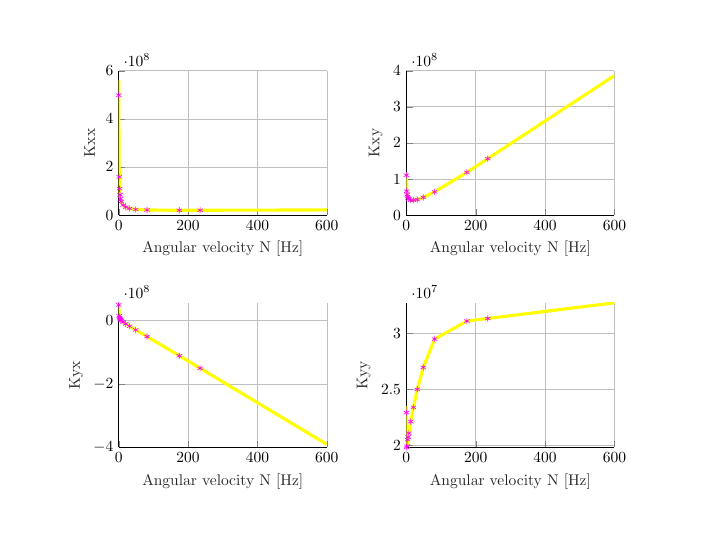
\begin{tikzpicture}[scale=0.56]

\begin{axis}[%
width=1.858in,
height=1.29in,
at={(0.813in,2.701in)},
scale only axis,
xmin=0,
xmax=600,
xlabel style={font=\color{white!15!black}},
xlabel={Angular velocity N [Hz]},
ymin=0,
ymax=600000000,
ylabel style={font=\color{white!15!black}},
ylabel={Kxx},
axis background/.style={fill=white},
axis x line*=bottom,
axis y line*=left,
xmajorgrids,
ymajorgrids
]
\addplot [color=mycolor1, only marks, mark=asterisk, mark options={solid, mycolor1}, forget plot]
  table[row sep=crcr]{%
234.77841101293	20367835.8276\\
174.508114226054	20137690.79\\
81.5421662410681	21633633.5344\\
48.8465150429587	23820011.3916\\
31.4350959711944	27502331.9932\\
20.3658453848465	33255957.9332\\
12.7237293216739	42001469.362\\
7.3663696072849	56615679.2496\\
5.31796736354792	67892786.092\\
3.64773168788546	84578301.318\\
2.29263481895177	110009327.9728\\
1.24085905149452	158800075.944\\
0.196567830697068	498264006.404\\
};
\addplot [color=mycolor2, line width=2.0pt, forget plot]
  table[row sep=crcr]{%
0	562161592.71088\\
1.0016694490818	236552565.808063\\
2.00333889816361	123429454.958988\\
3.00500834724541	96640254.0700133\\
4.00667779632721	80992459.6041695\\
5.00834724540902	70985865.2728369\\
6.01001669449082	64082834.0822733\\
7.01168614357262	58568324.6969214\\
8.01335559265442	54850782.0822265\\
9.01502504173623	52118352.6118736\\
10.016694490818	49385923.1415206\\
11.0183639398998	46653493.6711677\\
12.0200333889816	43921064.2008148\\
13.0217028380634	41660473.3902662\\
14.0233722871452	40514179.4132563\\
15.025041736227	39367885.4362465\\
16.0267111853088	38221591.4592367\\
17.0283806343907	37075297.4822269\\
18.0300500834725	35929003.5052171\\
19.0317195325543	34782709.5282072\\
20.0333889816361	33636415.5511974\\
21.0350584307179	32908111.3007585\\
22.0367278797997	32387458.9512083\\
23.0383973288815	31866806.601658\\
24.0400667779633	31346154.2521078\\
25.0417362270451	30825501.9025575\\
26.0434056761269	30304849.5530072\\
27.0450751252087	29784197.203457\\
28.0467445742905	29263544.8539067\\
29.0484140233723	28742892.5043565\\
30.0500834724541	28222240.1548062\\
31.0517529215359	27701587.805256\\
32.0534223706177	27371562.8680802\\
33.0550918196995	27159720.9709238\\
34.0567612687813	26947879.0737674\\
35.0584307178631	26736037.176611\\
36.0601001669449	26524195.2794547\\
37.0617696160267	26312353.3822983\\
38.0634390651085	26100511.4851419\\
39.0651085141903	25888669.5879855\\
40.0667779632721	25676827.6908292\\
41.0684474123539	25464985.7936728\\
42.0701168614357	25253143.8965164\\
43.0717863105175	25041301.99936\\
44.0734557595993	24829460.1022037\\
45.0751252086811	24617618.2050473\\
46.0767946577629	24405776.3078909\\
47.0784641068447	24193934.4107345\\
48.0801335559265	23982092.5135782\\
49.0818030050083	23804277.5440869\\
50.0834724540901	23737295.3056713\\
51.085141903172	23670313.0672557\\
52.0868113522538	23603330.82884\\
53.0884808013356	23536348.5904244\\
54.0901502504174	23469366.3520088\\
55.0918196994992	23402384.1135931\\
56.093489148581	23335401.8751775\\
57.0951585976628	23268419.6367619\\
58.0968280467446	23201437.3983462\\
59.0984974958264	23134455.1599306\\
60.1001669449082	23067472.921515\\
61.10183639399	23000490.6830993\\
62.1035058430718	22933508.4446837\\
63.1051752921536	22866526.2062681\\
64.1068447412354	22799543.9678524\\
65.1085141903172	22732561.7294368\\
66.110183639399	22665579.4910212\\
67.1118530884808	22598597.2526055\\
68.1135225375626	22531615.0141899\\
69.1151919866444	22464632.7757743\\
70.1168614357262	22397650.5373586\\
71.118530884808	22330668.298943\\
72.1202003338898	22263686.0605274\\
73.1218697829716	22196703.8221117\\
74.1235392320534	22129721.5836961\\
75.1252086811352	22062739.3452805\\
76.126878130217	21995757.1068648\\
77.1285475792988	21928774.8684492\\
78.1302170283806	21861792.6300336\\
79.1318864774624	21794810.3916179\\
80.1335559265442	21727828.1532023\\
81.135225375626	21660845.9147867\\
82.1368948247079	21624063.5797137\\
83.1385642737897	21607945.4184179\\
84.1402337228715	21591827.2571221\\
85.1419031719533	21575709.0958262\\
86.1435726210351	21559590.9345304\\
87.1452420701169	21543472.7732346\\
88.1469115191987	21527354.6119388\\
89.1485809682805	21511236.450643\\
90.1502504173623	21495118.2893471\\
91.1519198664441	21479000.1280513\\
92.1535893155259	21462881.9667555\\
93.1552587646077	21446763.8054597\\
94.1569282136895	21430645.6441638\\
95.1585976627713	21414527.482868\\
96.1602671118531	21398409.3215722\\
97.1619365609349	21382291.1602764\\
98.1636060100167	21366172.9989806\\
99.1652754590985	21350054.8376847\\
100.16694490818	21333936.6763889\\
101.168614357262	21317818.5150931\\
102.170283806344	21301700.3537973\\
103.171953255426	21285582.1925014\\
104.173622704508	21269464.0312056\\
105.175292153589	21253345.8699098\\
106.176961602671	21237227.708614\\
107.178631051753	21221109.5473181\\
108.180300500835	21204991.3860223\\
109.181969949917	21188873.2247265\\
110.183639398998	21172755.0634307\\
111.18530884808	21156636.9021349\\
112.186978297162	21140518.740839\\
113.188647746244	21124400.5795432\\
114.190317195326	21108282.4182474\\
115.191986644407	21092164.2569516\\
116.193656093489	21076046.0956557\\
117.195325542571	21059927.9343599\\
118.196994991653	21043809.7730641\\
119.198664440735	21027691.6117683\\
120.200333889816	21011573.4504725\\
121.202003338898	20995455.2891766\\
122.20367278798	20979337.1278808\\
123.205342237062	20963218.966585\\
124.207011686144	20947100.8052892\\
125.208681135225	20930982.6439933\\
126.210350584307	20914864.4826975\\
127.212020033389	20898746.3214017\\
128.213689482471	20882628.1601059\\
129.215358931553	20866509.99881\\
130.217028380634	20850391.8375142\\
131.218697829716	20834273.6762184\\
132.220367278798	20818155.5149226\\
133.22203672788	20802037.3536268\\
134.223706176962	20785919.1923309\\
135.225375626043	20769801.0310351\\
136.227045075125	20753682.8697393\\
137.228714524207	20737564.7084435\\
138.230383973289	20721446.5471476\\
139.232053422371	20705328.3858518\\
140.233722871452	20689210.224556\\
141.235392320534	20673092.0632602\\
142.237061769616	20656973.9019644\\
143.238731218698	20640855.7406685\\
144.24040066778	20624737.5793727\\
145.242070116861	20608619.4180769\\
146.243739565943	20592501.2567811\\
147.245409015025	20576383.0954852\\
148.247078464107	20560264.9341894\\
149.248747913189	20544146.7728936\\
150.25041736227	20528028.6115978\\
151.252086811352	20511910.450302\\
152.253756260434	20495792.2890061\\
153.255425709516	20479674.1277103\\
154.257095158598	20463555.9664145\\
155.258764607679	20447437.8051187\\
156.260434056761	20431319.6438228\\
157.262103505843	20415201.482527\\
158.263772954925	20399083.3212312\\
159.265442404007	20382965.1599354\\
160.267111853088	20366846.9986395\\
161.26878130217	20350728.8373437\\
162.270450751252	20334610.6760479\\
163.272120200334	20318492.5147521\\
164.273789649416	20302374.3534563\\
165.275459098497	20286256.1921604\\
166.277128547579	20270138.0308646\\
167.278797996661	20254019.8695688\\
168.280467445743	20237901.708273\\
169.282136894825	20221783.5469771\\
170.283806343907	20205665.3856813\\
171.285475792988	20189547.2243855\\
172.28714524207	20173429.0630897\\
173.288814691152	20157310.9017939\\
174.290484140234	20141192.740498\\
175.292153589316	20140684.6821551\\
176.293823038397	20144509.6052982\\
177.295492487479	20148334.5284413\\
178.297161936561	20152159.4515844\\
179.298831385643	20155984.3747275\\
180.300500834725	20159809.2978706\\
181.302170283806	20163634.2210137\\
182.303839732888	20167459.1441568\\
183.30550918197	20171284.0672999\\
184.307178631052	20175108.990443\\
185.308848080134	20178933.9135861\\
186.310517529215	20182758.8367292\\
187.312186978297	20186583.7598723\\
188.313856427379	20190408.6830154\\
189.315525876461	20194233.6061585\\
190.317195325543	20198058.5293016\\
191.318864774624	20201883.4524447\\
192.320534223706	20205708.3755878\\
193.322203672788	20209533.298731\\
194.32387312187	20213358.2218741\\
195.325542570952	20217183.1450172\\
196.327212020033	20221008.0681603\\
197.328881469115	20224832.9913034\\
198.330550918197	20228657.9144465\\
199.332220367279	20232482.8375896\\
200.333889816361	20236307.7607327\\
201.335559265442	20240132.6838758\\
202.337228714524	20243957.6070189\\
203.338898163606	20247782.530162\\
204.340567612688	20251607.4533051\\
205.34223706177	20255432.3764482\\
206.343906510851	20259257.2995913\\
207.345575959933	20263082.2227344\\
208.347245409015	20266907.1458775\\
209.348914858097	20270732.0690206\\
210.350584307179	20274556.9921637\\
211.35225375626	20278381.9153068\\
212.353923205342	20282206.8384499\\
213.355592654424	20286031.761593\\
214.357262103506	20289856.6847361\\
215.358931552588	20293681.6078792\\
216.360601001669	20297506.5310223\\
217.362270450751	20301331.4541654\\
218.363939899833	20305156.3773085\\
219.365609348915	20308981.3004516\\
220.367278797997	20312806.2235947\\
221.368948247078	20316631.1467378\\
222.37061769616	20320456.0698809\\
223.372287145242	20324280.993024\\
224.373956594324	20328105.9161671\\
225.375626043406	20331930.8393102\\
226.377295492487	20335755.7624533\\
227.378964941569	20339580.6855964\\
228.380634390651	20343405.6087395\\
229.382303839733	20347230.5318826\\
230.383973288815	20351055.4550257\\
231.385642737896	20354880.3781688\\
232.387312186978	20358705.3013119\\
233.38898163606	20362530.224455\\
234.390651085142	20366355.1475981\\
235.392320534224	20370180.0707412\\
236.393989983306	20374004.9938843\\
237.395659432387	20377829.9170274\\
238.397328881469	20381654.8401705\\
239.398998330551	20385479.7633136\\
240.400667779633	20389304.6864567\\
241.402337228715	20393129.6095998\\
242.404006677796	20396954.5327429\\
243.405676126878	20400779.455886\\
244.40734557596	20404604.3790291\\
245.409015025042	20408429.3021722\\
246.410684474124	20412254.2253153\\
247.412353923205	20416079.1484584\\
248.414023372287	20419904.0716015\\
249.415692821369	20423728.9947446\\
250.417362270451	20427553.9178877\\
251.419031719533	20431378.8410308\\
252.420701168614	20435203.7641739\\
253.422370617696	20439028.687317\\
254.424040066778	20442853.6104601\\
255.42570951586	20446678.5336032\\
256.427378964942	20450503.4567463\\
257.429048414023	20454328.3798894\\
258.430717863105	20458153.3030325\\
259.432387312187	20461978.2261756\\
260.434056761269	20465803.1493187\\
261.435726210351	20469628.0724618\\
262.437395659432	20473452.9956049\\
263.439065108514	20477277.918748\\
264.440734557596	20481102.8418911\\
265.442404006678	20484927.7650342\\
266.44407345576	20488752.6881773\\
267.445742904841	20492577.6113204\\
268.447412353923	20496402.5344635\\
269.449081803005	20500227.4576066\\
270.450751252087	20504052.3807497\\
271.452420701169	20507877.3038928\\
272.45409015025	20511702.2270359\\
273.455759599332	20515527.1501791\\
274.457429048414	20519352.0733221\\
275.459098497496	20523176.9964653\\
276.460767946578	20527001.9196084\\
277.462437395659	20530826.8427515\\
278.464106844741	20534651.7658946\\
279.465776293823	20538476.6890377\\
280.467445742905	20542301.6121808\\
281.469115191987	20546126.5353239\\
282.470784641068	20549951.458467\\
283.47245409015	20553776.3816101\\
284.474123539232	20557601.3047532\\
285.475792988314	20561426.2278963\\
286.477462437396	20565251.1510394\\
287.479131886477	20569076.0741825\\
288.480801335559	20572900.9973256\\
289.482470784641	20576725.9204687\\
290.484140233723	20580550.8436118\\
291.485809682805	20584375.7667549\\
292.487479131886	20588200.689898\\
293.489148580968	20592025.6130411\\
294.49081803005	20595850.5361842\\
295.492487479132	20599675.4593273\\
296.494156928214	20603500.3824704\\
297.495826377295	20607325.3056135\\
298.497495826377	20611150.2287566\\
299.499165275459	20614975.1518997\\
300.500834724541	20618800.0750428\\
301.502504173623	20622624.9981859\\
302.504173622705	20626449.921329\\
303.505843071786	20630274.8444721\\
304.507512520868	20634099.7676152\\
305.50918196995	20637924.6907583\\
306.510851419032	20641749.6139014\\
307.512520868114	20645574.5370445\\
308.514190317195	20649399.4601876\\
309.515859766277	20653224.3833307\\
310.517529215359	20657049.3064738\\
311.519198664441	20660874.2296169\\
312.520868113523	20664699.15276\\
313.522537562604	20668524.0759031\\
314.524207011686	20672348.9990462\\
315.525876460768	20676173.9221893\\
316.52754590985	20679998.8453324\\
317.529215358932	20683823.7684755\\
318.530884808013	20687648.6916186\\
319.532554257095	20691473.6147617\\
320.534223706177	20695298.5379048\\
321.535893155259	20699123.4610479\\
322.537562604341	20702948.384191\\
323.539232053422	20706773.3073341\\
324.540901502504	20710598.2304772\\
325.542570951586	20714423.1536203\\
326.544240400668	20718248.0767634\\
327.54590984975	20722072.9999065\\
328.547579298831	20725897.9230496\\
329.549248747913	20729722.8461927\\
330.550918196995	20733547.7693358\\
331.552587646077	20737372.6924789\\
332.554257095159	20741197.615622\\
333.55592654424	20745022.5387651\\
334.557595993322	20748847.4619082\\
335.559265442404	20752672.3850513\\
336.560934891486	20756497.3081944\\
337.562604340568	20760322.2313375\\
338.564273789649	20764147.1544806\\
339.565943238731	20767972.0776237\\
340.567612687813	20771797.0007668\\
341.569282136895	20775621.9239099\\
342.570951585977	20779446.847053\\
343.572621035058	20783271.7701961\\
344.57429048414	20787096.6933392\\
345.575959933222	20790921.6164823\\
346.577629382304	20794746.5396254\\
347.579298831386	20798571.4627685\\
348.580968280467	20802396.3859116\\
349.582637729549	20806221.3090547\\
350.584307178631	20810046.2321978\\
351.585976627713	20813871.1553409\\
352.587646076795	20817696.078484\\
353.589315525876	20821521.0016271\\
354.590984974958	20825345.9247702\\
355.59265442404	20829170.8479133\\
356.594323873122	20832995.7710564\\
357.595993322204	20836820.6941996\\
358.597662771285	20840645.6173426\\
359.599332220367	20844470.5404858\\
360.601001669449	20848295.4636289\\
361.602671118531	20852120.386772\\
362.604340567613	20855945.3099151\\
363.606010016694	20859770.2330582\\
364.607679465776	20863595.1562013\\
365.609348914858	20867420.0793444\\
366.61101836394	20871245.0024875\\
367.612687813022	20875069.9256306\\
368.614357262104	20878894.8487737\\
369.616026711185	20882719.7719168\\
370.617696160267	20886544.6950599\\
371.619365609349	20890369.618203\\
372.621035058431	20894194.5413461\\
373.622704507513	20898019.4644892\\
374.624373956594	20901844.3876323\\
375.626043405676	20905669.3107754\\
376.627712854758	20909494.2339185\\
377.62938230384	20913319.1570616\\
378.631051752922	20917144.0802047\\
379.632721202003	20920969.0033478\\
380.634390651085	20924793.9264909\\
381.636060100167	20928618.849634\\
382.637729549249	20932443.7727771\\
383.639398998331	20936268.6959202\\
384.641068447412	20940093.6190633\\
385.642737896494	20943918.5422064\\
386.644407345576	20947743.4653495\\
387.646076794658	20951568.3884926\\
388.64774624374	20955393.3116357\\
389.649415692821	20959218.2347788\\
390.651085141903	20963043.1579219\\
391.652754590985	20966868.081065\\
392.654424040067	20970693.0042081\\
393.656093489149	20974517.9273512\\
394.65776293823	20978342.8504943\\
395.659432387312	20982167.7736374\\
396.661101836394	20985992.6967805\\
397.662771285476	20989817.6199236\\
398.664440734558	20993642.5430667\\
399.666110183639	20997467.4662098\\
400.667779632721	21001292.3893529\\
401.669449081803	21005117.312496\\
402.671118530885	21008942.2356391\\
403.672787979967	21012767.1587822\\
404.674457429048	21016592.0819253\\
405.67612687813	21020417.0050684\\
406.677796327212	21024241.9282115\\
407.679465776294	21028066.8513546\\
408.681135225376	21031891.7744977\\
409.682804674457	21035716.6976408\\
410.684474123539	21039541.6207839\\
411.686143572621	21043366.543927\\
412.687813021703	21047191.4670701\\
413.689482470785	21051016.3902132\\
414.691151919866	21054841.3133563\\
415.692821368948	21058666.2364994\\
416.69449081803	21062491.1596425\\
417.696160267112	21066316.0827856\\
418.697829716194	21070141.0059287\\
419.699499165275	21073965.9290718\\
420.701168614357	21077790.8522149\\
421.702838063439	21081615.775358\\
422.704507512521	21085440.6985011\\
423.706176961603	21089265.6216442\\
424.707846410684	21093090.5447873\\
425.709515859766	21096915.4679304\\
426.711185308848	21100740.3910735\\
427.71285475793	21104565.3142166\\
428.714524207012	21108390.2373597\\
429.716193656093	21112215.1605028\\
430.717863105175	21116040.0836459\\
431.719532554257	21119865.006789\\
432.721202003339	21123689.9299321\\
433.722871452421	21127514.8530752\\
434.724540901503	21131339.7762183\\
435.726210350584	21135164.6993615\\
436.727879799666	21138989.6225046\\
437.729549248748	21142814.5456477\\
438.73121869783	21146639.4687907\\
439.732888146912	21150464.3919339\\
440.734557595993	21154289.315077\\
441.736227045075	21158114.2382201\\
442.737896494157	21161939.1613632\\
443.739565943239	21165764.0845063\\
444.741235392321	21169589.0076494\\
445.742904841402	21173413.9307925\\
446.744574290484	21177238.8539356\\
447.746243739566	21181063.7770787\\
448.747913188648	21184888.7002218\\
449.74958263773	21188713.6233649\\
450.751252086811	21192538.546508\\
451.752921535893	21196363.4696511\\
452.754590984975	21200188.3927942\\
453.756260434057	21204013.3159373\\
454.757929883139	21207838.2390804\\
455.75959933222	21211663.1622235\\
456.761268781302	21215488.0853666\\
457.762938230384	21219313.0085097\\
458.764607679466	21223137.9316528\\
459.766277128548	21226962.8547959\\
460.767946577629	21230787.777939\\
461.769616026711	21234612.7010821\\
462.771285475793	21238437.6242252\\
463.772954924875	21242262.5473683\\
464.774624373957	21246087.4705114\\
465.776293823038	21249912.3936545\\
466.77796327212	21253737.3167976\\
467.779632721202	21257562.2399407\\
468.781302170284	21261387.1630838\\
469.782971619366	21265212.0862269\\
470.784641068447	21269037.00937\\
471.786310517529	21272861.9325131\\
472.787979966611	21276686.8556562\\
473.789649415693	21280511.7787993\\
474.791318864775	21284336.7019424\\
475.792988313856	21288161.6250855\\
476.794657762938	21291986.5482286\\
477.79632721202	21295811.4713717\\
478.797996661102	21299636.3945148\\
479.799666110184	21303461.3176579\\
480.801335559265	21307286.240801\\
481.803005008347	21311111.1639441\\
482.804674457429	21314936.0870872\\
483.806343906511	21318761.0102303\\
484.808013355593	21322585.9333734\\
485.809682804674	21326410.8565165\\
486.811352253756	21330235.7796596\\
487.813021702838	21334060.7028027\\
488.81469115192	21337885.6259458\\
489.816360601002	21341710.5490889\\
490.818030050083	21345535.472232\\
491.819699499165	21349360.3953751\\
492.821368948247	21353185.3185182\\
493.823038397329	21357010.2416613\\
494.824707846411	21360835.1648044\\
495.826377295492	21364660.0879475\\
496.828046744574	21368485.0110906\\
497.829716193656	21372309.9342337\\
498.831385642738	21376134.8573768\\
499.83305509182	21379959.7805199\\
500.834724540902	21383784.703663\\
501.836393989983	21387609.6268061\\
502.838063439065	21391434.5499492\\
503.839732888147	21395259.4730923\\
504.841402337229	21399084.3962354\\
505.843071786311	21402909.3193785\\
506.844741235392	21406734.2425216\\
507.846410684474	21410559.1656647\\
508.848080133556	21414384.0888078\\
509.849749582638	21418209.0119509\\
510.85141903172	21422033.935094\\
511.853088480801	21425858.8582371\\
512.854757929883	21429683.7813803\\
513.856427378965	21433508.7045233\\
514.858096828047	21437333.6276664\\
515.859766277129	21441158.5508096\\
516.86143572621	21444983.4739526\\
517.863105175292	21448808.3970957\\
518.864774624374	21452633.3202389\\
519.866444073456	21456458.2433819\\
520.868113522538	21460283.1665251\\
521.869782971619	21464108.0896682\\
522.871452420701	21467933.0128113\\
523.873121869783	21471757.9359544\\
524.874791318865	21475582.8590974\\
525.876460767947	21479407.7822406\\
526.878130217028	21483232.7053837\\
527.87979966611	21487057.6285268\\
528.881469115192	21490882.5516698\\
529.883138564274	21494707.474813\\
530.884808013356	21498532.3979561\\
531.886477462437	21502357.3210992\\
532.888146911519	21506182.2442423\\
533.889816360601	21510007.1673854\\
534.891485809683	21513832.0905285\\
535.893155258765	21517657.0136716\\
536.894824707846	21521481.9368147\\
537.896494156928	21525306.8599578\\
538.89816360601	21529131.7831009\\
539.899833055092	21532956.706244\\
540.901502504174	21536781.6293871\\
541.903171953255	21540606.5525302\\
542.904841402337	21544431.4756733\\
543.906510851419	21548256.3988164\\
544.908180300501	21552081.3219595\\
545.909849749583	21555906.2451026\\
546.911519198664	21559731.1682457\\
547.913188647746	21563556.0913888\\
548.914858096828	21567381.0145319\\
549.91652754591	21571205.937675\\
550.918196994992	21575030.8608181\\
551.919866444073	21578855.7839612\\
552.921535893155	21582680.7071043\\
553.923205342237	21586505.6302474\\
554.924874791319	21590330.5533905\\
555.926544240401	21594155.4765336\\
556.928213689483	21597980.3996767\\
557.929883138564	21601805.3228198\\
558.931552587646	21605630.2459629\\
559.933222036728	21609455.169106\\
560.93489148581	21613280.0922491\\
561.936560934892	21617105.0153922\\
562.938230383973	21620929.9385353\\
563.939899833055	21624754.8616784\\
564.941569282137	21628579.7848215\\
565.943238731219	21632404.7079646\\
566.9449081803	21636229.6311077\\
567.946577629382	21640054.5542508\\
568.948247078464	21643879.4773939\\
569.949916527546	21647704.400537\\
570.951585976628	21651529.3236801\\
571.953255425709	21655354.2468232\\
572.954924874791	21659179.1699663\\
573.956594323873	21663004.0931094\\
574.958263772955	21666829.0162525\\
575.959933222037	21670653.9393956\\
576.961602671118	21674478.8625387\\
577.9632721202	21678303.7856818\\
578.964941569282	21682128.7088249\\
579.966611018364	21685953.631968\\
580.968280467446	21689778.5551111\\
581.969949916528	21693603.4782542\\
582.971619365609	21697428.4013973\\
583.973288814691	21701253.3245404\\
584.974958263773	21705078.2476835\\
585.976627712855	21708903.1708266\\
586.978297161937	21712728.0939697\\
587.979966611018	21716553.0171128\\
588.9816360601	21720377.9402559\\
589.983305509182	21724202.863399\\
590.984974958264	21728027.7865421\\
591.986644407346	21731852.7096852\\
592.988313856427	21735677.6328283\\
593.989983305509	21739502.5559714\\
594.991652754591	21743327.4791145\\
595.993322203673	21747152.4022576\\
596.994991652755	21750977.3254007\\
597.996661101836	21754802.2485438\\
598.998330550918	21758627.1716869\\
600	21762452.09483\\
};
\end{axis}

\begin{axis}[%
width=1.858in,
height=1.29in,
at={(3.381in,2.701in)},
scale only axis,
xmin=0,
xmax=600,
xlabel style={font=\color{white!15!black}},
xlabel={Angular velocity N [Hz]},
ymin=0,
ymax=400000000,
ylabel style={font=\color{white!15!black}},
ylabel={Kxy},
axis background/.style={fill=white},
axis x line*=bottom,
axis y line*=left,
xmajorgrids,
ymajorgrids
]
\addplot [color=mycolor1, only marks, mark=asterisk, mark options={solid, mycolor1}, forget plot]
  table[row sep=crcr]{%
234.77841101293	156498625.568\\
174.508114226054	118524694.364\\
81.5421662410681	64785828.0844\\
48.8465150429587	49135965.5276\\
31.4350959711944	43152194.55\\
20.3658453848465	41080889.2116\\
12.7237293216739	41656251.8056\\
7.3663696072849	44648137.2944\\
5.31796736354792	47294805.2268\\
3.64773168788546	51322343.3848\\
2.29263481895177	56615679.2496\\
1.24085905149452	66281770.8288\\
0.196567830697068	110584690.5668\\
};
\addplot [color=mycolor2, line width=2.0pt, forget plot]
  table[row sep=crcr]{%
0	118923867.084817\\
1.0016694490818	76429129.6754659\\
2.00333889816361	59274383.652524\\
3.00500834724541	53832976.0843141\\
4.00667779632721	50456795.3849099\\
5.00834724540902	48041410.5463124\\
6.01001669449082	46400632.8163539\\
7.01168614357262	45106411.2259142\\
8.01335559265442	44286819.7640716\\
9.01502504173623	43727424.754393\\
10.016694490818	43168029.7447145\\
11.0183639398998	42608634.7350359\\
12.0200333889816	42049239.7253574\\
13.0217028380634	41633817.8600912\\
14.0233722871452	41558403.7826563\\
15.025041736227	41482989.7052215\\
16.0267111853088	41407575.6277866\\
17.0283806343907	41332161.5503518\\
18.0300500834725	41256747.4729169\\
19.0317195325543	41181333.395482\\
20.0333889816361	41105919.3180472\\
21.0350584307179	41206113.9992789\\
22.0367278797997	41393548.845117\\
23.0383973288815	41580983.6909551\\
24.0400667779633	41768418.5367932\\
25.0417362270451	41955853.3826313\\
26.0434056761269	42143288.2284694\\
27.0450751252087	42330723.0743075\\
28.0467445742905	42518157.9201456\\
29.0484140233723	42705592.7659837\\
30.0500834724541	42893027.6118217\\
31.0517529215359	43080462.4576598\\
32.0534223706177	43364694.3783197\\
33.0550918196995	43708937.4611989\\
34.0567612687813	44053180.544078\\
35.0584307178631	44397423.6269571\\
36.0601001669449	44741666.7098362\\
37.0617696160267	45085909.7927153\\
38.0634390651085	45430152.8755944\\
39.0651085141903	45774395.9584735\\
40.0667779632721	46118639.0413526\\
41.0684474123539	46462882.1242317\\
42.0701168614357	46807125.2071108\\
43.0717863105175	47151368.2899899\\
44.0734557595993	47495611.3728691\\
45.0751252086811	47839854.4557482\\
46.0767946577629	48184097.5386273\\
47.0784641068447	48528340.6215064\\
48.0801335559265	48872583.7043855\\
49.0818030050083	49248586.751904\\
50.0834724540901	49728038.5637211\\
51.085141903172	50207490.3755383\\
52.0868113522538	50686942.1873555\\
53.0884808013356	51166393.9991726\\
54.0901502504174	51645845.8109898\\
55.0918196994992	52125297.622807\\
56.093489148581	52604749.4346241\\
57.0951585976628	53084201.2464413\\
58.0968280467446	53563653.0582585\\
59.0984974958264	54043104.8700757\\
60.1001669449082	54522556.6818928\\
61.10183639399	55002008.49371\\
62.1035058430718	55481460.3055272\\
63.1051752921536	55960912.1173443\\
64.1068447412354	56440363.9291615\\
65.1085141903172	56919815.7409787\\
66.110183639399	57399267.5527958\\
67.1118530884808	57878719.364613\\
68.1135225375626	58358171.1764302\\
69.1151919866444	58837622.9882474\\
70.1168614357262	59317074.8000645\\
71.118530884808	59796526.6118817\\
72.1202003338898	60275978.4236989\\
73.1218697829716	60755430.235516\\
74.1235392320534	61234882.0473332\\
75.1252086811352	61714333.8591504\\
76.126878130217	62193785.6709675\\
77.1285475792988	62673237.4827847\\
78.1302170283806	63152689.2946019\\
79.1318864774624	63632141.1064191\\
80.1335559265442	64111592.9182362\\
81.135225375626	64591044.7300534\\
82.1368948247079	65129610.3027455\\
83.1385642737897	65708624.2508339\\
84.1402337228715	66287638.1989223\\
85.1419031719533	66866652.1470107\\
86.1435726210351	67445666.0950991\\
87.1452420701169	68024680.0431875\\
88.1469115191987	68603693.9912759\\
89.1485809682805	69182707.9393643\\
90.1502504173623	69761721.8874527\\
91.1519198664441	70340735.8355411\\
92.1535893155259	70919749.7836295\\
93.1552587646077	71498763.7317179\\
94.1569282136895	72077777.6798063\\
95.1585976627713	72656791.6278947\\
96.1602671118531	73235805.5759831\\
97.1619365609349	73814819.5240715\\
98.1636060100167	74393833.4721599\\
99.1652754590985	74972847.4202483\\
100.16694490818	75551861.3683367\\
101.168614357262	76130875.3164251\\
102.170283806344	76709889.2645135\\
103.171953255426	77288903.2126019\\
104.173622704508	77867917.1606903\\
105.175292153589	78446931.1087787\\
106.176961602671	79025945.0568671\\
107.178631051753	79604959.0049555\\
108.180300500835	80183972.9530439\\
109.181969949917	80762986.9011323\\
110.183639398998	81342000.8492207\\
111.18530884808	81921014.7973091\\
112.186978297162	82500028.7453975\\
113.188647746244	83079042.6934859\\
114.190317195326	83658056.6415743\\
115.191986644407	84237070.5896627\\
116.193656093489	84816084.5377511\\
117.195325542571	85395098.4858395\\
118.196994991653	85974112.4339279\\
119.198664440735	86553126.3820163\\
120.200333889816	87132140.3301047\\
121.202003338898	87711154.2781931\\
122.20367278798	88290168.2262815\\
123.205342237062	88869182.1743699\\
124.207011686144	89448196.1224583\\
125.208681135225	90027210.0705467\\
126.210350584307	90606224.0186351\\
127.212020033389	91185237.9667235\\
128.213689482471	91764251.9148119\\
129.215358931553	92343265.8629003\\
130.217028380634	92922279.8109888\\
131.218697829716	93501293.7590771\\
132.220367278798	94080307.7071655\\
133.22203672788	94659321.6552539\\
134.223706176962	95238335.6033423\\
135.225375626043	95817349.5514308\\
136.227045075125	96396363.4995191\\
137.228714524207	96975377.4476075\\
138.230383973289	97554391.3956959\\
139.232053422371	98133405.3437844\\
140.233722871452	98712419.2918727\\
141.235392320534	99291433.2399611\\
142.237061769616	99870447.1880496\\
143.238731218698	100449461.136138\\
144.24040066778	101028475.084226\\
145.242070116861	101607489.032315\\
146.243739565943	102186502.980403\\
147.245409015025	102765516.928492\\
148.247078464107	103344530.87658\\
149.248747913189	103923544.824668\\
150.25041736227	104502558.772757\\
151.252086811352	105081572.720845\\
152.253756260434	105660586.668934\\
153.255425709516	106239600.617022\\
154.257095158598	106818614.56511\\
155.258764607679	107397628.513199\\
156.260434056761	107976642.461287\\
157.262103505843	108555656.409376\\
158.263772954925	109134670.357464\\
159.265442404007	109713684.305552\\
160.267111853088	110292698.253641\\
161.26878130217	110871712.201729\\
162.270450751252	111450726.149818\\
163.272120200334	112029740.097906\\
164.273789649416	112608754.045994\\
165.275459098497	113187767.994083\\
166.277128547579	113766781.942171\\
167.278797996661	114345795.89026\\
168.280467445743	114924809.838348\\
169.282136894825	115503823.786436\\
170.283806343907	116082837.734525\\
171.285475792988	116661851.682613\\
172.28714524207	117240865.630702\\
173.288814691152	117819879.57879\\
174.290484140234	118398893.526878\\
175.292153589316	119018686.569597\\
176.293823038397	119649798.888208\\
177.295492487479	120280911.20682\\
178.297161936561	120912023.525432\\
179.298831385643	121543135.844044\\
180.300500834725	122174248.162655\\
181.302170283806	122805360.481267\\
182.303839732888	123436472.799879\\
183.30550918197	124067585.11849\\
184.307178631052	124698697.437102\\
185.308848080134	125329809.755714\\
186.310517529215	125960922.074325\\
187.312186978297	126592034.392937\\
188.313856427379	127223146.711549\\
189.315525876461	127854259.030161\\
190.317195325543	128485371.348772\\
191.318864774624	129116483.667384\\
192.320534223706	129747595.985996\\
193.322203672788	130378708.304607\\
194.32387312187	131009820.623219\\
195.325542570952	131640932.941831\\
196.327212020033	132272045.260442\\
197.328881469115	132903157.579054\\
198.330550918197	133534269.897666\\
199.332220367279	134165382.216278\\
200.333889816361	134796494.534889\\
201.335559265442	135427606.853501\\
202.337228714524	136058719.172113\\
203.338898163606	136689831.490724\\
204.340567612688	137320943.809336\\
205.34223706177	137952056.127948\\
206.343906510851	138583168.446559\\
207.345575959933	139214280.765171\\
208.347245409015	139845393.083783\\
209.348914858097	140476505.402395\\
210.350584307179	141107617.721006\\
211.35225375626	141738730.039618\\
212.353923205342	142369842.35823\\
213.355592654424	143000954.676841\\
214.357262103506	143632066.995453\\
215.358931552588	144263179.314065\\
216.360601001669	144894291.632676\\
217.362270450751	145525403.951288\\
218.363939899833	146156516.2699\\
219.365609348915	146787628.588512\\
220.367278797997	147418740.907123\\
221.368948247078	148049853.225735\\
222.37061769616	148680965.544347\\
223.372287145242	149312077.862958\\
224.373956594324	149943190.18157\\
225.375626043406	150574302.500182\\
226.377295492487	151205414.818793\\
227.378964941569	151836527.137405\\
228.380634390651	152467639.456017\\
229.382303839733	153098751.774629\\
230.383973288815	153729864.09324\\
231.385642737896	154360976.411852\\
232.387312186978	154992088.730464\\
233.38898163606	155623201.049075\\
234.390651085142	156254313.367687\\
235.392320534224	156885425.686299\\
236.393989983306	157516538.004911\\
237.395659432387	158147650.323522\\
238.397328881469	158778762.642134\\
239.398998330551	159409874.960746\\
240.400667779633	160040987.279357\\
241.402337228715	160672099.597969\\
242.404006677796	161303211.916581\\
243.405676126878	161934324.235192\\
244.40734557596	162565436.553804\\
245.409015025042	163196548.872416\\
246.410684474124	163827661.191027\\
247.412353923205	164458773.509639\\
248.414023372287	165089885.828251\\
249.415692821369	165720998.146863\\
250.417362270451	166352110.465474\\
251.419031719533	166983222.784086\\
252.420701168614	167614335.102698\\
253.422370617696	168245447.421309\\
254.424040066778	168876559.739921\\
255.42570951586	169507672.058533\\
256.427378964942	170138784.377145\\
257.429048414023	170769896.695756\\
258.430717863105	171401009.014368\\
259.432387312187	172032121.33298\\
260.434056761269	172663233.651591\\
261.435726210351	173294345.970203\\
262.437395659432	173925458.288815\\
263.439065108514	174556570.607426\\
264.440734557596	175187682.926038\\
265.442404006678	175818795.24465\\
266.44407345576	176449907.563262\\
267.445742904841	177081019.881873\\
268.447412353923	177712132.200485\\
269.449081803005	178343244.519097\\
270.450751252087	178974356.837708\\
271.452420701169	179605469.15632\\
272.45409015025	180236581.474932\\
273.455759599332	180867693.793543\\
274.457429048414	181498806.112155\\
275.459098497496	182129918.430767\\
276.460767946578	182761030.749379\\
277.462437395659	183392143.06799\\
278.464106844741	184023255.386602\\
279.465776293823	184654367.705214\\
280.467445742905	185285480.023825\\
281.469115191987	185916592.342437\\
282.470784641068	186547704.661049\\
283.47245409015	187178816.97966\\
284.474123539232	187809929.298272\\
285.475792988314	188441041.616884\\
286.477462437396	189072153.935496\\
287.479131886477	189703266.254107\\
288.480801335559	190334378.572719\\
289.482470784641	190965490.891331\\
290.484140233723	191596603.209942\\
291.485809682805	192227715.528554\\
292.487479131886	192858827.847166\\
293.489148580968	193489940.165777\\
294.49081803005	194121052.484389\\
295.492487479132	194752164.803001\\
296.494156928214	195383277.121613\\
297.495826377295	196014389.440224\\
298.497495826377	196645501.758836\\
299.499165275459	197276614.077448\\
300.500834724541	197907726.396059\\
301.502504173623	198538838.714671\\
302.504173622705	199169951.033283\\
303.505843071786	199801063.351894\\
304.507512520868	200432175.670506\\
305.50918196995	201063287.989118\\
306.510851419032	201694400.30773\\
307.512520868114	202325512.626341\\
308.514190317195	202956624.944953\\
309.515859766277	203587737.263565\\
310.517529215359	204218849.582176\\
311.519198664441	204849961.900788\\
312.520868113523	205481074.2194\\
313.522537562604	206112186.538011\\
314.524207011686	206743298.856623\\
315.525876460768	207374411.175235\\
316.52754590985	208005523.493847\\
317.529215358932	208636635.812458\\
318.530884808013	209267748.13107\\
319.532554257095	209898860.449682\\
320.534223706177	210529972.768293\\
321.535893155259	211161085.086905\\
322.537562604341	211792197.405517\\
323.539232053422	212423309.724128\\
324.540901502504	213054422.04274\\
325.542570951586	213685534.361352\\
326.544240400668	214316646.679964\\
327.54590984975	214947758.998575\\
328.547579298831	215578871.317187\\
329.549248747913	216209983.635799\\
330.550918196995	216841095.95441\\
331.552587646077	217472208.273022\\
332.554257095159	218103320.591634\\
333.55592654424	218734432.910246\\
334.557595993322	219365545.228857\\
335.559265442404	219996657.547469\\
336.560934891486	220627769.866081\\
337.562604340568	221258882.184692\\
338.564273789649	221889994.503304\\
339.565943238731	222521106.821916\\
340.567612687813	223152219.140527\\
341.569282136895	223783331.459139\\
342.570951585977	224414443.777751\\
343.572621035058	225045556.096363\\
344.57429048414	225676668.414974\\
345.575959933222	226307780.733586\\
346.577629382304	226938893.052198\\
347.579298831386	227570005.370809\\
348.580968280467	228201117.689421\\
349.582637729549	228832230.008033\\
350.584307178631	229463342.326644\\
351.585976627713	230094454.645256\\
352.587646076795	230725566.963868\\
353.589315525876	231356679.282479\\
354.590984974958	231987791.601091\\
355.59265442404	232618903.919703\\
356.594323873122	233250016.238315\\
357.595993322204	233881128.556926\\
358.597662771285	234512240.875538\\
359.599332220367	235143353.19415\\
360.601001669449	235774465.512761\\
361.602671118531	236405577.831373\\
362.604340567613	237036690.149985\\
363.606010016694	237667802.468596\\
364.607679465776	238298914.787208\\
365.609348914858	238930027.10582\\
366.61101836394	239561139.424432\\
367.612687813022	240192251.743043\\
368.614357262104	240823364.061655\\
369.616026711185	241454476.380267\\
370.617696160267	242085588.698878\\
371.619365609349	242716701.01749\\
372.621035058431	243347813.336102\\
373.622704507513	243978925.654714\\
374.624373956594	244610037.973325\\
375.626043405676	245241150.291937\\
376.627712854758	245872262.610549\\
377.62938230384	246503374.92916\\
378.631051752922	247134487.247772\\
379.632721202003	247765599.566384\\
380.634390651085	248396711.884995\\
381.636060100167	249027824.203607\\
382.637729549249	249658936.522219\\
383.639398998331	250290048.840831\\
384.641068447412	250921161.159442\\
385.642737896494	251552273.478054\\
386.644407345576	252183385.796666\\
387.646076794658	252814498.115277\\
388.64774624374	253445610.433889\\
389.649415692821	254076722.752501\\
390.651085141903	254707835.071112\\
391.652754590985	255338947.389724\\
392.654424040067	255970059.708336\\
393.656093489149	256601172.026948\\
394.65776293823	257232284.345559\\
395.659432387312	257863396.664171\\
396.661101836394	258494508.982783\\
397.662771285476	259125621.301394\\
398.664440734558	259756733.620006\\
399.666110183639	260387845.938618\\
400.667779632721	261018958.257229\\
401.669449081803	261650070.575841\\
402.671118530885	262281182.894453\\
403.672787979967	262912295.213065\\
404.674457429048	263543407.531676\\
405.67612687813	264174519.850288\\
406.677796327212	264805632.1689\\
407.679465776294	265436744.487511\\
408.681135225376	266067856.806123\\
409.682804674457	266698969.124735\\
410.684474123539	267330081.443347\\
411.686143572621	267961193.761958\\
412.687813021703	268592306.08057\\
413.689482470785	269223418.399182\\
414.691151919866	269854530.717793\\
415.692821368948	270485643.036405\\
416.69449081803	271116755.355017\\
417.696160267112	271747867.673628\\
418.697829716194	272378979.99224\\
419.699499165275	273010092.310852\\
420.701168614357	273641204.629463\\
421.702838063439	274272316.948075\\
422.704507512521	274903429.266687\\
423.706176961603	275534541.585299\\
424.707846410684	276165653.90391\\
425.709515859766	276796766.222522\\
426.711185308848	277427878.541134\\
427.71285475793	278058990.859745\\
428.714524207012	278690103.178357\\
429.716193656093	279321215.496969\\
430.717863105175	279952327.815581\\
431.719532554257	280583440.134192\\
432.721202003339	281214552.452804\\
433.722871452421	281845664.771416\\
434.724540901503	282476777.090027\\
435.726210350584	283107889.408639\\
436.727879799666	283739001.727251\\
437.729549248748	284370114.045862\\
438.73121869783	285001226.364474\\
439.732888146912	285632338.683086\\
440.734557595993	286263451.001697\\
441.736227045075	286894563.320309\\
442.737896494157	287525675.638921\\
443.739565943239	288156787.957533\\
444.741235392321	288787900.276144\\
445.742904841402	289419012.594756\\
446.744574290484	290050124.913368\\
447.746243739566	290681237.231979\\
448.747913188648	291312349.550591\\
449.74958263773	291943461.869203\\
450.751252086811	292574574.187814\\
451.752921535893	293205686.506426\\
452.754590984975	293836798.825038\\
453.756260434057	294467911.14365\\
454.757929883139	295099023.462261\\
455.75959933222	295730135.780873\\
456.761268781302	296361248.099485\\
457.762938230384	296992360.418096\\
458.764607679466	297623472.736708\\
459.766277128548	298254585.05532\\
460.767946577629	298885697.373931\\
461.769616026711	299516809.692543\\
462.771285475793	300147922.011155\\
463.772954924875	300779034.329767\\
464.774624373957	301410146.648378\\
465.776293823038	302041258.96699\\
466.77796327212	302672371.285602\\
467.779632721202	303303483.604213\\
468.781302170284	303934595.922825\\
469.782971619366	304565708.241437\\
470.784641068447	305196820.560048\\
471.786310517529	305827932.87866\\
472.787979966611	306459045.197272\\
473.789649415693	307090157.515884\\
474.791318864775	307721269.834495\\
475.792988313856	308352382.153107\\
476.794657762938	308983494.471719\\
477.79632721202	309614606.79033\\
478.797996661102	310245719.108942\\
479.799666110184	310876831.427554\\
480.801335559265	311507943.746166\\
481.803005008347	312139056.064777\\
482.804674457429	312770168.383389\\
483.806343906511	313401280.702001\\
484.808013355593	314032393.020612\\
485.809682804674	314663505.339224\\
486.811352253756	315294617.657836\\
487.813021702838	315925729.976447\\
488.81469115192	316556842.295059\\
489.816360601002	317187954.613671\\
490.818030050083	317819066.932282\\
491.819699499165	318450179.250894\\
492.821368948247	319081291.569506\\
493.823038397329	319712403.888118\\
494.824707846411	320343516.206729\\
495.826377295492	320974628.525341\\
496.828046744574	321605740.843953\\
497.829716193656	322236853.162565\\
498.831385642738	322867965.481176\\
499.83305509182	323499077.799788\\
500.834724540902	324130190.1184\\
501.836393989983	324761302.437011\\
502.838063439065	325392414.755623\\
503.839732888147	326023527.074235\\
504.841402337229	326654639.392846\\
505.843071786311	327285751.711458\\
506.844741235392	327916864.03007\\
507.846410684474	328547976.348681\\
508.848080133556	329179088.667293\\
509.849749582638	329810200.985905\\
510.85141903172	330441313.304517\\
511.853088480801	331072425.623128\\
512.854757929883	331703537.94174\\
513.856427378965	332334650.260352\\
514.858096828047	332965762.578963\\
515.859766277129	333596874.897575\\
516.86143572621	334227987.216187\\
517.863105175292	334859099.534799\\
518.864774624374	335490211.85341\\
519.866444073456	336121324.172022\\
520.868113522538	336752436.490634\\
521.869782971619	337383548.809245\\
522.871452420701	338014661.127857\\
523.873121869783	338645773.446469\\
524.874791318865	339276885.76508\\
525.876460767947	339907998.083692\\
526.878130217028	340539110.402304\\
527.87979966611	341170222.720915\\
528.881469115192	341801335.039527\\
529.883138564274	342432447.358139\\
530.884808013356	343063559.676751\\
531.886477462437	343694671.995362\\
532.888146911519	344325784.313974\\
533.889816360601	344956896.632586\\
534.891485809683	345588008.951197\\
535.893155258765	346219121.269809\\
536.894824707846	346850233.588421\\
537.896494156928	347481345.907032\\
538.89816360601	348112458.225644\\
539.899833055092	348743570.544256\\
540.901502504174	349374682.862868\\
541.903171953255	350005795.181479\\
542.904841402337	350636907.500091\\
543.906510851419	351268019.818703\\
544.908180300501	351899132.137314\\
545.909849749583	352530244.455926\\
546.911519198664	353161356.774538\\
547.913188647746	353792469.093149\\
548.914858096828	354423581.411761\\
549.91652754591	355054693.730373\\
550.918196994992	355685806.048984\\
551.919866444073	356316918.367596\\
552.921535893155	356948030.686208\\
553.923205342237	357579143.00482\\
554.924874791319	358210255.323431\\
555.926544240401	358841367.642043\\
556.928213689483	359472479.960655\\
557.929883138564	360103592.279266\\
558.931552587646	360734704.597878\\
559.933222036728	361365816.91649\\
560.93489148581	361996929.235102\\
561.936560934892	362628041.553713\\
562.938230383973	363259153.872325\\
563.939899833055	363890266.190937\\
564.941569282137	364521378.509548\\
565.943238731219	365152490.82816\\
566.9449081803	365783603.146772\\
567.946577629382	366414715.465384\\
568.948247078464	367045827.783995\\
569.949916527546	367676940.102607\\
570.951585976628	368308052.421219\\
571.953255425709	368939164.73983\\
572.954924874791	369570277.058442\\
573.956594323873	370201389.377054\\
574.958263772955	370832501.695665\\
575.959933222037	371463614.014277\\
576.961602671118	372094726.332889\\
577.9632721202	372725838.651501\\
578.964941569282	373356950.970112\\
579.966611018364	373988063.288724\\
580.968280467446	374619175.607336\\
581.969949916528	375250287.925947\\
582.971619365609	375881400.244559\\
583.973288814691	376512512.563171\\
584.974958263773	377143624.881783\\
585.976627712855	377774737.200394\\
586.978297161937	378405849.519006\\
587.979966611018	379036961.837617\\
588.9816360601	379668074.156229\\
589.983305509182	380299186.474841\\
590.984974958264	380930298.793453\\
591.986644407346	381561411.112064\\
592.988313856427	382192523.430676\\
593.989983305509	382823635.749288\\
594.991652754591	383454748.067899\\
595.993322203673	384085860.386511\\
596.994991652755	384716972.705123\\
597.996661101836	385348085.023735\\
598.998330550918	385979197.342346\\
600	386610309.660958\\
};
\end{axis}

\begin{axis}[%
width=1.858in,
height=1.29in,
at={(0.813in,0.628in)},
scale only axis,
xmin=0,
xmax=600,
xlabel style={font=\color{white!15!black}},
xlabel={Angular velocity N [Hz]},
ymin=-400000000,
ymax=55562273.0307247,
ylabel style={font=\color{white!15!black}},
ylabel={Kyx},
axis background/.style={fill=white},
axis x line*=bottom,
axis y line*=left,
xmajorgrids,
ymajorgrids
]
\addplot [color=mycolor1, only marks, mark=asterisk, mark options={solid, mycolor1}, forget plot]
  table[row sep=crcr]{%
234.77841101293	-150744999.628\\
174.508114226054	-111160053.1608\\
81.5421662410681	-50746980.7908\\
48.8465150429587	-29458564.8128\\
31.4350959711944	-18066385.4516\\
20.3658453848465	-10632700.73712\\
12.7237293216739	-4913596.55276\\
7.3663696072849	270420.41918\\
5.31796736354792	2968870.98504\\
3.64773168788546	6064321.74076\\
2.29263481895177	9263337.7634\\
1.24085905149452	14268992.3312\\
0.196567830697068	49020893.0088\\
};
\addplot [color=mycolor2, line width=2.0pt, forget plot]
  table[row sep=crcr]{%
0	55562273.0307247\\
1.0016694490818	22228738.7511821\\
2.00333889816361	10640166.8291999\\
3.00500834724541	7581617.15481416\\
4.00667779632721	5399086.27798732\\
5.00834724540902	3542690.50203664\\
6.01001669449082	2057203.89699824\\
7.01168614357262	737660.57978904\\
8.01335559265442	-355631.686254448\\
9.01502504173623	-1324891.11648594\\
10.016694490818	-2294150.54671744\\
11.0183639398998	-3263409.97694893\\
12.0200333889816	-4232669.40718042\\
13.0217028380634	-5136589.97111752\\
14.0233722871452	-5886205.90081999\\
15.025041736227	-6635821.83052247\\
16.0267111853088	-7385437.76022494\\
17.0283806343907	-8135053.68992741\\
18.0300500834725	-8884669.61962989\\
19.0317195325543	-9634285.54933236\\
20.0333889816361	-10383901.4790348\\
21.0350584307179	-11082118.5862344\\
22.0367278797997	-11754801.4218533\\
23.0383973288815	-12427484.2574722\\
24.0400667779633	-13100167.0930912\\
25.0417362270451	-13772849.9287101\\
26.0434056761269	-14445532.764329\\
27.0450751252087	-15118215.599948\\
28.0467445742905	-15790898.4355669\\
29.0484140233723	-16463581.2711858\\
30.0500834724541	-17136264.1068048\\
31.0517529215359	-17808946.9424237\\
32.0534223706177	-18470952.4324395\\
33.0550918196995	-19126338.3017671\\
34.0567612687813	-19781724.1710946\\
35.0584307178631	-20437110.0404221\\
36.0601001669449	-21092495.9097497\\
37.0617696160267	-21747881.7790772\\
38.0634390651085	-22403267.6484047\\
39.0651085141903	-23058653.5177323\\
40.0667779632721	-23714039.3870598\\
41.0684474123539	-24369425.2563873\\
42.0701168614357	-25024811.1257149\\
43.0717863105175	-25680196.9950424\\
44.0734557595993	-26335582.8643699\\
45.0751252086811	-26990968.7336975\\
46.0767946577629	-27646354.603025\\
47.0784641068447	-28301740.4723526\\
48.0801335559265	-28957126.3416801\\
49.0818030050083	-29611762.8017429\\
50.0834724540901	-30263958.281053\\
51.085141903172	-30916153.7603631\\
52.0868113522538	-31568349.2396733\\
53.0884808013356	-32220544.7189834\\
54.0901502504174	-32872740.1982935\\
55.0918196994992	-33524935.6776036\\
56.093489148581	-34177131.1569137\\
57.0951585976628	-34829326.6362239\\
58.0968280467446	-35481522.115534\\
59.0984974958264	-36133717.5948441\\
60.1001669449082	-36785913.0741542\\
61.10183639399	-37438108.5534643\\
62.1035058430718	-38090304.0327745\\
63.1051752921536	-38742499.5120846\\
64.1068447412354	-39394694.9913947\\
65.1085141903172	-40046890.4707048\\
66.110183639399	-40699085.9500149\\
67.1118530884808	-41351281.4293251\\
68.1135225375626	-42003476.9086352\\
69.1151919866444	-42655672.3879453\\
70.1168614357262	-43307867.8672554\\
71.118530884808	-43960063.3465656\\
72.1202003338898	-44612258.8258757\\
73.1218697829716	-45264454.3051858\\
74.1235392320534	-45916649.7844959\\
75.1252086811352	-46568845.263806\\
76.126878130217	-47221040.7431162\\
77.1285475792988	-47873236.2224263\\
78.1302170283806	-48525431.7017364\\
79.1318864774624	-49177627.1810465\\
80.1335559265442	-49829822.6603566\\
81.135225375626	-50482018.1396668\\
82.1368948247079	-51133459.7300535\\
83.1385642737897	-51784385.4746925\\
84.1402337228715	-52435311.2193315\\
85.1419031719533	-53086236.9639705\\
86.1435726210351	-53737162.7086095\\
87.1452420701169	-54388088.4532485\\
88.1469115191987	-55039014.1978875\\
89.1485809682805	-55689939.9425265\\
90.1502504173623	-56340865.6871655\\
91.1519198664441	-56991791.4318045\\
92.1535893155259	-57642717.1764434\\
93.1552587646077	-58293642.9210824\\
94.1569282136895	-58944568.6657214\\
95.1585976627713	-59595494.4103604\\
96.1602671118531	-60246420.1549994\\
97.1619365609349	-60897345.8996384\\
98.1636060100167	-61548271.6442774\\
99.1652754590985	-62199197.3889164\\
100.16694490818	-62850123.1335554\\
101.168614357262	-63501048.8781944\\
102.170283806344	-64151974.6228334\\
103.171953255426	-64802900.3674724\\
104.173622704508	-65453826.1121114\\
105.175292153589	-66104751.8567504\\
106.176961602671	-66755677.6013893\\
107.178631051753	-67406603.3460284\\
108.180300500835	-68057529.0906674\\
109.181969949917	-68708454.8353063\\
110.183639398998	-69359380.5799454\\
111.18530884808	-70010306.3245843\\
112.186978297162	-70661232.0692233\\
113.188647746244	-71312157.8138623\\
114.190317195326	-71963083.5585013\\
115.191986644407	-72614009.3031403\\
116.193656093489	-73264935.0477793\\
117.195325542571	-73915860.7924183\\
118.196994991653	-74566786.5370573\\
119.198664440735	-75217712.2816963\\
120.200333889816	-75868638.0263353\\
121.202003338898	-76519563.7709743\\
122.20367278798	-77170489.5156133\\
123.205342237062	-77821415.2602523\\
124.207011686144	-78472341.0048913\\
125.208681135225	-79123266.7495303\\
126.210350584307	-79774192.4941693\\
127.212020033389	-80425118.2388082\\
128.213689482471	-81076043.9834473\\
129.215358931553	-81726969.7280862\\
130.217028380634	-82377895.4727252\\
131.218697829716	-83028821.2173642\\
132.220367278798	-83679746.9620032\\
133.22203672788	-84330672.7066422\\
134.223706176962	-84981598.4512812\\
135.225375626043	-85632524.1959202\\
136.227045075125	-86283449.9405592\\
137.228714524207	-86934375.6851982\\
138.230383973289	-87585301.4298372\\
139.232053422371	-88236227.1744762\\
140.233722871452	-88887152.9191152\\
141.235392320534	-89538078.6637542\\
142.237061769616	-90189004.4083932\\
143.238731218698	-90839930.1530322\\
144.24040066778	-91490855.8976711\\
145.242070116861	-92141781.6423102\\
146.243739565943	-92792707.3869492\\
147.245409015025	-93443633.1315881\\
148.247078464107	-94094558.8762271\\
149.248747913189	-94745484.6208661\\
150.25041736227	-95396410.3655051\\
151.252086811352	-96047336.1101441\\
152.253756260434	-96698261.8547831\\
153.255425709516	-97349187.5994221\\
154.257095158598	-98000113.3440611\\
155.258764607679	-98651039.0887001\\
156.260434056761	-99301964.8333391\\
157.262103505843	-99952890.5779781\\
158.263772954925	-100603816.322617\\
159.265442404007	-101254742.067256\\
160.267111853088	-101905667.811895\\
161.26878130217	-102556593.556534\\
162.270450751252	-103207519.301173\\
163.272120200334	-103858445.045812\\
164.273789649416	-104509370.790451\\
165.275459098497	-105160296.53509\\
166.277128547579	-105811222.279729\\
167.278797996661	-106462148.024368\\
168.280467445743	-107113073.769007\\
169.282136894825	-107763999.513646\\
170.283806343907	-108414925.258285\\
171.285475792988	-109065851.002924\\
172.28714524207	-109716776.747563\\
173.288814691152	-110367702.492202\\
174.290484140234	-111018628.236841\\
175.292153589316	-111675002.611483\\
176.293823038397	-112332889.392096\\
177.295492487479	-112990776.172709\\
178.297161936561	-113648662.953323\\
179.298831385643	-114306549.733936\\
180.300500834725	-114964436.51455\\
181.302170283806	-115622323.295163\\
182.303839732888	-116280210.075777\\
183.30550918197	-116938096.85639\\
184.307178631052	-117595983.637003\\
185.308848080134	-118253870.417617\\
186.310517529215	-118911757.19823\\
187.312186978297	-119569643.978844\\
188.313856427379	-120227530.759457\\
189.315525876461	-120885417.54007\\
190.317195325543	-121543304.320684\\
191.318864774624	-122201191.101297\\
192.320534223706	-122859077.881911\\
193.322203672788	-123516964.662524\\
194.32387312187	-124174851.443137\\
195.325542570952	-124832738.223751\\
196.327212020033	-125490625.004364\\
197.328881469115	-126148511.784978\\
198.330550918197	-126806398.565591\\
199.332220367279	-127464285.346205\\
200.333889816361	-128122172.126818\\
201.335559265442	-128780058.907431\\
202.337228714524	-129437945.688045\\
203.338898163606	-130095832.468658\\
204.340567612688	-130753719.249272\\
205.34223706177	-131411606.029885\\
206.343906510851	-132069492.810498\\
207.345575959933	-132727379.591112\\
208.347245409015	-133385266.371725\\
209.348914858097	-134043153.152339\\
210.350584307179	-134701039.932952\\
211.35225375626	-135358926.713565\\
212.353923205342	-136016813.494179\\
213.355592654424	-136674700.274792\\
214.357262103506	-137332587.055406\\
215.358931552588	-137990473.836019\\
216.360601001669	-138648360.616632\\
217.362270450751	-139306247.397246\\
218.363939899833	-139964134.177859\\
219.365609348915	-140622020.958473\\
220.367278797997	-141279907.739086\\
221.368948247078	-141937794.519699\\
222.37061769616	-142595681.300313\\
223.372287145242	-143253568.080926\\
224.373956594324	-143911454.86154\\
225.375626043406	-144569341.642153\\
226.377295492487	-145227228.422767\\
227.378964941569	-145885115.20338\\
228.380634390651	-146543001.983993\\
229.382303839733	-147200888.764607\\
230.383973288815	-147858775.54522\\
231.385642737896	-148516662.325834\\
232.387312186978	-149174549.106447\\
233.38898163606	-149832435.88706\\
234.390651085142	-150490322.667674\\
235.392320534224	-151148209.448287\\
236.393989983306	-151806096.228901\\
237.395659432387	-152463983.009514\\
238.397328881469	-153121869.790127\\
239.398998330551	-153779756.570741\\
240.400667779633	-154437643.351354\\
241.402337228715	-155095530.131968\\
242.404006677796	-155753416.912581\\
243.405676126878	-156411303.693194\\
244.40734557596	-157069190.473808\\
245.409015025042	-157727077.254421\\
246.410684474124	-158384964.035035\\
247.412353923205	-159042850.815648\\
248.414023372287	-159700737.596262\\
249.415692821369	-160358624.376875\\
250.417362270451	-161016511.157488\\
251.419031719533	-161674397.938102\\
252.420701168614	-162332284.718715\\
253.422370617696	-162990171.499329\\
254.424040066778	-163648058.279942\\
255.42570951586	-164305945.060555\\
256.427378964942	-164963831.841169\\
257.429048414023	-165621718.621782\\
258.430717863105	-166279605.402396\\
259.432387312187	-166937492.183009\\
260.434056761269	-167595378.963622\\
261.435726210351	-168253265.744236\\
262.437395659432	-168911152.524849\\
263.439065108514	-169569039.305463\\
264.440734557596	-170226926.086076\\
265.442404006678	-170884812.86669\\
266.44407345576	-171542699.647303\\
267.445742904841	-172200586.427916\\
268.447412353923	-172858473.20853\\
269.449081803005	-173516359.989143\\
270.450751252087	-174174246.769757\\
271.452420701169	-174832133.55037\\
272.45409015025	-175490020.330983\\
273.455759599332	-176147907.111597\\
274.457429048414	-176805793.89221\\
275.459098497496	-177463680.672824\\
276.460767946578	-178121567.453437\\
277.462437395659	-178779454.23405\\
278.464106844741	-179437341.014664\\
279.465776293823	-180095227.795277\\
280.467445742905	-180753114.575891\\
281.469115191987	-181411001.356504\\
282.470784641068	-182068888.137117\\
283.47245409015	-182726774.917731\\
284.474123539232	-183384661.698344\\
285.475792988314	-184042548.478958\\
286.477462437396	-184700435.259571\\
287.479131886477	-185358322.040185\\
288.480801335559	-186016208.820798\\
289.482470784641	-186674095.601411\\
290.484140233723	-187331982.382025\\
291.485809682805	-187989869.162638\\
292.487479131886	-188647755.943252\\
293.489148580968	-189305642.723865\\
294.49081803005	-189963529.504478\\
295.492487479132	-190621416.285092\\
296.494156928214	-191279303.065705\\
297.495826377295	-191937189.846319\\
298.497495826377	-192595076.626932\\
299.499165275459	-193252963.407545\\
300.500834724541	-193910850.188159\\
301.502504173623	-194568736.968772\\
302.504173622705	-195226623.749386\\
303.505843071786	-195884510.529999\\
304.507512520868	-196542397.310613\\
305.50918196995	-197200284.091226\\
306.510851419032	-197858170.871839\\
307.512520868114	-198516057.652453\\
308.514190317195	-199173944.433066\\
309.515859766277	-199831831.21368\\
310.517529215359	-200489717.994293\\
311.519198664441	-201147604.774906\\
312.520868113523	-201805491.55552\\
313.522537562604	-202463378.336133\\
314.524207011686	-203121265.116747\\
315.525876460768	-203779151.89736\\
316.52754590985	-204437038.677973\\
317.529215358932	-205094925.458587\\
318.530884808013	-205752812.2392\\
319.532554257095	-206410699.019814\\
320.534223706177	-207068585.800427\\
321.535893155259	-207726472.581041\\
322.537562604341	-208384359.361654\\
323.539232053422	-209042246.142267\\
324.540901502504	-209700132.922881\\
325.542570951586	-210358019.703494\\
326.544240400668	-211015906.484108\\
327.54590984975	-211673793.264721\\
328.547579298831	-212331680.045334\\
329.549248747913	-212989566.825948\\
330.550918196995	-213647453.606561\\
331.552587646077	-214305340.387175\\
332.554257095159	-214963227.167788\\
333.55592654424	-215621113.948401\\
334.557595993322	-216279000.729015\\
335.559265442404	-216936887.509628\\
336.560934891486	-217594774.290242\\
337.562604340568	-218252661.070855\\
338.564273789649	-218910547.851468\\
339.565943238731	-219568434.632082\\
340.567612687813	-220226321.412695\\
341.569282136895	-220884208.193309\\
342.570951585977	-221542094.973922\\
343.572621035058	-222199981.754535\\
344.57429048414	-222857868.535149\\
345.575959933222	-223515755.315762\\
346.577629382304	-224173642.096376\\
347.579298831386	-224831528.876989\\
348.580968280467	-225489415.657603\\
349.582637729549	-226147302.438216\\
350.584307178631	-226805189.218829\\
351.585976627713	-227463075.999443\\
352.587646076795	-228120962.780056\\
353.589315525876	-228778849.56067\\
354.590984974958	-229436736.341283\\
355.59265442404	-230094623.121896\\
356.594323873122	-230752509.90251\\
357.595993322204	-231410396.683123\\
358.597662771285	-232068283.463737\\
359.599332220367	-232726170.24435\\
360.601001669449	-233384057.024963\\
361.602671118531	-234041943.805577\\
362.604340567613	-234699830.58619\\
363.606010016694	-235357717.366804\\
364.607679465776	-236015604.147417\\
365.609348914858	-236673490.92803\\
366.61101836394	-237331377.708644\\
367.612687813022	-237989264.489257\\
368.614357262104	-238647151.269871\\
369.616026711185	-239305038.050484\\
370.617696160267	-239962924.831098\\
371.619365609349	-240620811.611711\\
372.621035058431	-241278698.392324\\
373.622704507513	-241936585.172938\\
374.624373956594	-242594471.953551\\
375.626043405676	-243252358.734165\\
376.627712854758	-243910245.514778\\
377.62938230384	-244568132.295391\\
378.631051752922	-245226019.076005\\
379.632721202003	-245883905.856618\\
380.634390651085	-246541792.637232\\
381.636060100167	-247199679.417845\\
382.637729549249	-247857566.198458\\
383.639398998331	-248515452.979072\\
384.641068447412	-249173339.759685\\
385.642737896494	-249831226.540299\\
386.644407345576	-250489113.320912\\
387.646076794658	-251147000.101525\\
388.64774624374	-251804886.882139\\
389.649415692821	-252462773.662752\\
390.651085141903	-253120660.443366\\
391.652754590985	-253778547.223979\\
392.654424040067	-254436434.004592\\
393.656093489149	-255094320.785206\\
394.65776293823	-255752207.565819\\
395.659432387312	-256410094.346433\\
396.661101836394	-257067981.127046\\
397.662771285476	-257725867.90766\\
398.664440734558	-258383754.688273\\
399.666110183639	-259041641.468886\\
400.667779632721	-259699528.2495\\
401.669449081803	-260357415.030113\\
402.671118530885	-261015301.810727\\
403.672787979967	-261673188.59134\\
404.674457429048	-262331075.371953\\
405.67612687813	-262988962.152567\\
406.677796327212	-263646848.93318\\
407.679465776294	-264304735.713794\\
408.681135225376	-264962622.494407\\
409.682804674457	-265620509.27502\\
410.684474123539	-266278396.055634\\
411.686143572621	-266936282.836247\\
412.687813021703	-267594169.616861\\
413.689482470785	-268252056.397474\\
414.691151919866	-268909943.178087\\
415.692821368948	-269567829.958701\\
416.69449081803	-270225716.739314\\
417.696160267112	-270883603.519928\\
418.697829716194	-271541490.300541\\
419.699499165275	-272199377.081155\\
420.701168614357	-272857263.861768\\
421.702838063439	-273515150.642381\\
422.704507512521	-274173037.422995\\
423.706176961603	-274830924.203608\\
424.707846410684	-275488810.984222\\
425.709515859766	-276146697.764835\\
426.711185308848	-276804584.545448\\
427.71285475793	-277462471.326062\\
428.714524207012	-278120358.106675\\
429.716193656093	-278778244.887289\\
430.717863105175	-279436131.667902\\
431.719532554257	-280094018.448515\\
432.721202003339	-280751905.229129\\
433.722871452421	-281409792.009742\\
434.724540901503	-282067678.790356\\
435.726210350584	-282725565.570969\\
436.727879799666	-283383452.351583\\
437.729549248748	-284041339.132196\\
438.73121869783	-284699225.912809\\
439.732888146912	-285357112.693423\\
440.734557595993	-286014999.474036\\
441.736227045075	-286672886.25465\\
442.737896494157	-287330773.035263\\
443.739565943239	-287988659.815876\\
444.741235392321	-288646546.59649\\
445.742904841402	-289304433.377103\\
446.744574290484	-289962320.157717\\
447.746243739566	-290620206.93833\\
448.747913188648	-291278093.718944\\
449.74958263773	-291935980.499557\\
450.751252086811	-292593867.28017\\
451.752921535893	-293251754.060784\\
452.754590984975	-293909640.841397\\
453.756260434057	-294567527.622011\\
454.757929883139	-295225414.402624\\
455.75959933222	-295883301.183237\\
456.761268781302	-296541187.963851\\
457.762938230384	-297199074.744464\\
458.764607679466	-297856961.525078\\
459.766277128548	-298514848.305691\\
460.767946577629	-299172735.086304\\
461.769616026711	-299830621.866918\\
462.771285475793	-300488508.647531\\
463.772954924875	-301146395.428145\\
464.774624373957	-301804282.208758\\
465.776293823038	-302462168.989371\\
466.77796327212	-303120055.769985\\
467.779632721202	-303777942.550598\\
468.781302170284	-304435829.331212\\
469.782971619366	-305093716.111825\\
470.784641068447	-305751602.892439\\
471.786310517529	-306409489.673052\\
472.787979966611	-307067376.453665\\
473.789649415693	-307725263.234279\\
474.791318864775	-308383150.014892\\
475.792988313856	-309041036.795506\\
476.794657762938	-309698923.576119\\
477.79632721202	-310356810.356732\\
478.797996661102	-311014697.137346\\
479.799666110184	-311672583.917959\\
480.801335559265	-312330470.698573\\
481.803005008347	-312988357.479186\\
482.804674457429	-313646244.259799\\
483.806343906511	-314304131.040413\\
484.808013355593	-314962017.821026\\
485.809682804674	-315619904.60164\\
486.811352253756	-316277791.382253\\
487.813021702838	-316935678.162866\\
488.81469115192	-317593564.94348\\
489.816360601002	-318251451.724093\\
490.818030050083	-318909338.504707\\
491.819699499165	-319567225.28532\\
492.821368948247	-320225112.065933\\
493.823038397329	-320882998.846547\\
494.824707846411	-321540885.62716\\
495.826377295492	-322198772.407774\\
496.828046744574	-322856659.188387\\
497.829716193656	-323514545.969001\\
498.831385642738	-324172432.749614\\
499.83305509182	-324830319.530227\\
500.834724540902	-325488206.310841\\
501.836393989983	-326146093.091454\\
502.838063439065	-326803979.872068\\
503.839732888147	-327461866.652681\\
504.841402337229	-328119753.433294\\
505.843071786311	-328777640.213908\\
506.844741235392	-329435526.994521\\
507.846410684474	-330093413.775135\\
508.848080133556	-330751300.555748\\
509.849749582638	-331409187.336361\\
510.85141903172	-332067074.116975\\
511.853088480801	-332724960.897588\\
512.854757929883	-333382847.678202\\
513.856427378965	-334040734.458815\\
514.858096828047	-334698621.239429\\
515.859766277129	-335356508.020042\\
516.86143572621	-336014394.800655\\
517.863105175292	-336672281.581269\\
518.864774624374	-337330168.361882\\
519.866444073456	-337988055.142496\\
520.868113522538	-338645941.923109\\
521.869782971619	-339303828.703722\\
522.871452420701	-339961715.484336\\
523.873121869783	-340619602.264949\\
524.874791318865	-341277489.045563\\
525.876460767947	-341935375.826176\\
526.878130217028	-342593262.606789\\
527.87979966611	-343251149.387403\\
528.881469115192	-343909036.168016\\
529.883138564274	-344566922.94863\\
530.884808013356	-345224809.729243\\
531.886477462437	-345882696.509856\\
532.888146911519	-346540583.29047\\
533.889816360601	-347198470.071083\\
534.891485809683	-347856356.851697\\
535.893155258765	-348514243.63231\\
536.894824707846	-349172130.412924\\
537.896494156928	-349830017.193537\\
538.89816360601	-350487903.97415\\
539.899833055092	-351145790.754764\\
540.901502504174	-351803677.535377\\
541.903171953255	-352461564.315991\\
542.904841402337	-353119451.096604\\
543.906510851419	-353777337.877217\\
544.908180300501	-354435224.657831\\
545.909849749583	-355093111.438444\\
546.911519198664	-355750998.219058\\
547.913188647746	-356408884.999671\\
548.914858096828	-357066771.780284\\
549.91652754591	-357724658.560898\\
550.918196994992	-358382545.341511\\
551.919866444073	-359040432.122125\\
552.921535893155	-359698318.902738\\
553.923205342237	-360356205.683351\\
554.924874791319	-361014092.463965\\
555.926544240401	-361671979.244578\\
556.928213689483	-362329866.025192\\
557.929883138564	-362987752.805805\\
558.931552587646	-363645639.586419\\
559.933222036728	-364303526.367032\\
560.93489148581	-364961413.147645\\
561.936560934892	-365619299.928259\\
562.938230383973	-366277186.708872\\
563.939899833055	-366935073.489485\\
564.941569282137	-367592960.270099\\
565.943238731219	-368250847.050712\\
566.9449081803	-368908733.831326\\
567.946577629382	-369566620.611939\\
568.948247078464	-370224507.392553\\
569.949916527546	-370882394.173166\\
570.951585976628	-371540280.953779\\
571.953255425709	-372198167.734393\\
572.954924874791	-372856054.515006\\
573.956594323873	-373513941.295619\\
574.958263772955	-374171828.076233\\
575.959933222037	-374829714.856847\\
576.961602671118	-375487601.63746\\
577.9632721202	-376145488.418073\\
578.964941569282	-376803375.198687\\
579.966611018364	-377461261.9793\\
580.968280467446	-378119148.759914\\
581.969949916528	-378777035.540527\\
582.971619365609	-379434922.32114\\
583.973288814691	-380092809.101754\\
584.974958263773	-380750695.882367\\
585.976627712855	-381408582.662981\\
586.978297161937	-382066469.443594\\
587.979966611018	-382724356.224207\\
588.9816360601	-383382243.004821\\
589.983305509182	-384040129.785434\\
590.984974958264	-384698016.566047\\
591.986644407346	-385355903.346661\\
592.988313856427	-386013790.127274\\
593.989983305509	-386671676.907888\\
594.991652754591	-387329563.688501\\
595.993322203673	-387987450.469115\\
596.994991652755	-388645337.249728\\
597.996661101836	-389303224.030341\\
598.998330550918	-389961110.810955\\
600	-390618997.591568\\
};
\end{axis}

\begin{axis}[%
width=1.858in,
height=1.29in,
at={(3.381in,0.628in)},
scale only axis,
xmin=0,
xmax=600,
xlabel style={font=\color{white!15!black}},
xlabel={Angular velocity N [Hz]},
ymin=19792473.2336,
ymax=32694341.38083,
ylabel style={font=\color{white!15!black}},
ylabel={Kyy},
axis background/.style={fill=white},
axis x line*=bottom,
axis y line*=left,
xmajorgrids,
ymajorgrids
]
\addplot [color=mycolor1, only marks, mark=asterisk, mark options={solid, mycolor1}, forget plot]
  table[row sep=crcr]{%
234.77841101293	31299725.1136\\
174.508114226054	31069580.076\\
81.5421662410681	29458564.8128\\
48.8465150429587	26926969.3992\\
31.4350959711944	24970736.5796\\
20.3658453848465	23359721.3164\\
12.7237293216739	22093923.6096\\
7.3663696072849	21058270.9404\\
5.31796736354792	20713053.384\\
3.64773168788546	20482908.3464\\
2.29263481895177	19907545.7524\\
1.24085905149452	19792473.2336\\
0.196567830697068	22899431.2412\\
};
\addplot [color=mycolor2, line width=2.0pt, forget plot]
  table[row sep=crcr]{%
0	23484256.6073986\\
1.0016694490818	20504106.1916779\\
2.00333889816361	19875894.509508\\
3.00500834724541	20210013.4877572\\
4.00667779632721	20532368.232108\\
5.00834724540902	20670390.222885\\
6.01001669449082	20829684.5679712\\
7.01168614357262	20998496.0797677\\
8.01335559265442	21183342.393206\\
9.01502504173623	21376979.1273255\\
10.016694490818	21570615.861445\\
11.0183639398998	21764252.5955645\\
12.0200333889816	21957889.329684\\
13.0217028380634	22143278.2897194\\
14.0233722871452	22309189.260076\\
15.025041736227	22475100.2304327\\
16.0267111853088	22641011.2007894\\
17.0283806343907	22806922.1711461\\
18.0300500834725	22972833.1415028\\
19.0317195325543	23138744.1118595\\
20.0333889816361	23304655.0822162\\
21.0350584307179	23457118.3734836\\
22.0367278797997	23602901.0313577\\
23.0383973288815	23748683.6892317\\
24.0400667779633	23894466.3471058\\
25.0417362270451	24040249.0049799\\
26.0434056761269	24186031.662854\\
27.0450751252087	24331814.320728\\
28.0467445742905	24477596.9786021\\
29.0484140233723	24623379.6364762\\
30.0500834724541	24769162.2943503\\
31.0517529215359	24914944.9522243\\
32.0534223706177	25040207.6773199\\
33.0550918196995	25152748.6851842\\
34.0567612687813	25265289.6930486\\
35.0584307178631	25377830.7009129\\
36.0601001669449	25490371.7087772\\
37.0617696160267	25602912.7166415\\
38.0634390651085	25715453.7245059\\
39.0651085141903	25827994.7323702\\
40.0667779632721	25940535.7402345\\
41.0684474123539	26053076.7480988\\
42.0701168614357	26165617.7559632\\
43.0717863105175	26278158.7638275\\
44.0734557595993	26390699.7716918\\
45.0751252086811	26503240.7795561\\
46.0767946577629	26615781.7874205\\
47.0784641068447	26728322.7952848\\
48.0801335559265	26840863.8031491\\
49.0818030050083	26945187.5384256\\
50.0834724540901	27022745.919749\\
51.085141903172	27100304.3010724\\
52.0868113522538	27177862.6823957\\
53.0884808013356	27255421.0637191\\
54.0901502504174	27332979.4450425\\
55.0918196994992	27410537.8263658\\
56.093489148581	27488096.2076892\\
57.0951585976628	27565654.5890126\\
58.0968280467446	27643212.9703359\\
59.0984974958264	27720771.3516593\\
60.1001669449082	27798329.7329827\\
61.10183639399	27875888.114306\\
62.1035058430718	27953446.4956294\\
63.1051752921536	28031004.8769528\\
64.1068447412354	28108563.2582761\\
65.1085141903172	28186121.6395995\\
66.110183639399	28263680.0209229\\
67.1118530884808	28341238.4022462\\
68.1135225375626	28418796.7835696\\
69.1151919866444	28496355.164893\\
70.1168614357262	28573913.5462163\\
71.118530884808	28651471.9275397\\
72.1202003338898	28729030.3088631\\
73.1218697829716	28806588.6901864\\
74.1235392320534	28884147.0715098\\
75.1252086811352	28961705.4528331\\
76.126878130217	29039263.8341565\\
77.1285475792988	29116822.2154799\\
78.1302170283806	29194380.5968032\\
79.1318864774624	29271938.9781266\\
80.1335559265442	29349497.35945\\
81.135225375626	29427055.7407733\\
82.1368948247079	29468870.9178468\\
83.1385642737897	29486228.9377038\\
84.1402337228715	29503586.9575608\\
85.1419031719533	29520944.9774179\\
86.1435726210351	29538302.9972749\\
87.1452420701169	29555661.017132\\
88.1469115191987	29573019.036989\\
89.1485809682805	29590377.056846\\
90.1502504173623	29607735.0767031\\
91.1519198664441	29625093.0965601\\
92.1535893155259	29642451.1164172\\
93.1552587646077	29659809.1362742\\
94.1569282136895	29677167.1561312\\
95.1585976627713	29694525.1759883\\
96.1602671118531	29711883.1958453\\
97.1619365609349	29729241.2157024\\
98.1636060100167	29746599.2355594\\
99.1652754590985	29763957.2554164\\
100.16694490818	29781315.2752735\\
101.168614357262	29798673.2951305\\
102.170283806344	29816031.3149875\\
103.171953255426	29833389.3348446\\
104.173622704508	29850747.3547016\\
105.175292153589	29868105.3745587\\
106.176961602671	29885463.3944157\\
107.178631051753	29902821.4142727\\
108.180300500835	29920179.4341298\\
109.181969949917	29937537.4539868\\
110.183639398998	29954895.4738439\\
111.18530884808	29972253.4937009\\
112.186978297162	29989611.513558\\
113.188647746244	30006969.533415\\
114.190317195326	30024327.553272\\
115.191986644407	30041685.5731291\\
116.193656093489	30059043.5929861\\
117.195325542571	30076401.6128431\\
118.196994991653	30093759.6327002\\
119.198664440735	30111117.6525572\\
120.200333889816	30128475.6724143\\
121.202003338898	30145833.6922713\\
122.20367278798	30163191.7121283\\
123.205342237062	30180549.7319854\\
124.207011686144	30197907.7518424\\
125.208681135225	30215265.7716995\\
126.210350584307	30232623.7915565\\
127.212020033389	30249981.8114135\\
128.213689482471	30267339.8312706\\
129.215358931553	30284697.8511276\\
130.217028380634	30302055.8709847\\
131.218697829716	30319413.8908417\\
132.220367278798	30336771.9106987\\
133.22203672788	30354129.9305558\\
134.223706176962	30371487.9504128\\
135.225375626043	30388845.9702699\\
136.227045075125	30406203.9901269\\
137.228714524207	30423562.0099839\\
138.230383973289	30440920.029841\\
139.232053422371	30458278.049698\\
140.233722871452	30475636.0695551\\
141.235392320534	30492994.0894121\\
142.237061769616	30510352.1092691\\
143.238731218698	30527710.1291262\\
144.24040066778	30545068.1489832\\
145.242070116861	30562426.1688403\\
146.243739565943	30579784.1886973\\
147.245409015025	30597142.2085543\\
148.247078464107	30614500.2284114\\
149.248747913189	30631858.2482684\\
150.25041736227	30649216.2681255\\
151.252086811352	30666574.2879825\\
152.253756260434	30683932.3078396\\
153.255425709516	30701290.3276966\\
154.257095158598	30718648.3475536\\
155.258764607679	30736006.3674107\\
156.260434056761	30753364.3872677\\
157.262103505843	30770722.4071247\\
158.263772954925	30788080.4269818\\
159.265442404007	30805438.4468388\\
160.267111853088	30822796.4666959\\
161.26878130217	30840154.4865529\\
162.270450751252	30857512.5064099\\
163.272120200334	30874870.526267\\
164.273789649416	30892228.546124\\
165.275459098497	30909586.5659811\\
166.277128547579	30926944.5858381\\
167.278797996661	30944302.6056951\\
168.280467445743	30961660.6255522\\
169.282136894825	30979018.6454092\\
170.283806343907	30996376.6652663\\
171.285475792988	31013734.6851233\\
172.28714524207	31031092.7049803\\
173.288814691152	31048450.7248374\\
174.290484140234	31065808.7446944\\
175.292153589316	31072573.9681551\\
176.293823038397	31076398.8912982\\
177.295492487479	31080223.8144413\\
178.297161936561	31084048.7375844\\
179.298831385643	31087873.6607275\\
180.300500834725	31091698.5838706\\
181.302170283806	31095523.5070137\\
182.303839732888	31099348.4301568\\
183.30550918197	31103173.3532999\\
184.307178631052	31106998.276443\\
185.308848080134	31110823.1995861\\
186.310517529215	31114648.1227292\\
187.312186978297	31118473.0458723\\
188.313856427379	31122297.9690154\\
189.315525876461	31126122.8921585\\
190.317195325543	31129947.8153016\\
191.318864774624	31133772.7384447\\
192.320534223706	31137597.6615878\\
193.322203672788	31141422.584731\\
194.32387312187	31145247.5078741\\
195.325542570952	31149072.4310172\\
196.327212020033	31152897.3541603\\
197.328881469115	31156722.2773034\\
198.330550918197	31160547.2004465\\
199.332220367279	31164372.1235896\\
200.333889816361	31168197.0467327\\
201.335559265442	31172021.9698758\\
202.337228714524	31175846.8930189\\
203.338898163606	31179671.816162\\
204.340567612688	31183496.7393051\\
205.34223706177	31187321.6624482\\
206.343906510851	31191146.5855913\\
207.345575959933	31194971.5087344\\
208.347245409015	31198796.4318775\\
209.348914858097	31202621.3550206\\
210.350584307179	31206446.2781637\\
211.35225375626	31210271.2013068\\
212.353923205342	31214096.1244499\\
213.355592654424	31217921.047593\\
214.357262103506	31221745.9707361\\
215.358931552588	31225570.8938792\\
216.360601001669	31229395.8170223\\
217.362270450751	31233220.7401654\\
218.363939899833	31237045.6633085\\
219.365609348915	31240870.5864516\\
220.367278797997	31244695.5095947\\
221.368948247078	31248520.4327378\\
222.37061769616	31252345.3558809\\
223.372287145242	31256170.279024\\
224.373956594324	31259995.2021671\\
225.375626043406	31263820.1253102\\
226.377295492487	31267645.0484533\\
227.378964941569	31271469.9715964\\
228.380634390651	31275294.8947395\\
229.382303839733	31279119.8178826\\
230.383973288815	31282944.7410257\\
231.385642737896	31286769.6641688\\
232.387312186978	31290594.5873119\\
233.38898163606	31294419.510455\\
234.390651085142	31298244.4335981\\
235.392320534224	31302069.3567412\\
236.393989983306	31305894.2798843\\
237.395659432387	31309719.2030274\\
238.397328881469	31313544.1261705\\
239.398998330551	31317369.0493136\\
240.400667779633	31321193.9724567\\
241.402337228715	31325018.8955998\\
242.404006677796	31328843.8187429\\
243.405676126878	31332668.741886\\
244.40734557596	31336493.6650291\\
245.409015025042	31340318.5881722\\
246.410684474124	31344143.5113153\\
247.412353923205	31347968.4344584\\
248.414023372287	31351793.3576015\\
249.415692821369	31355618.2807446\\
250.417362270451	31359443.2038877\\
251.419031719533	31363268.1270308\\
252.420701168614	31367093.0501739\\
253.422370617696	31370917.973317\\
254.424040066778	31374742.8964601\\
255.42570951586	31378567.8196032\\
256.427378964942	31382392.7427463\\
257.429048414023	31386217.6658894\\
258.430717863105	31390042.5890325\\
259.432387312187	31393867.5121756\\
260.434056761269	31397692.4353187\\
261.435726210351	31401517.3584618\\
262.437395659432	31405342.2816049\\
263.439065108514	31409167.204748\\
264.440734557596	31412992.1278911\\
265.442404006678	31416817.0510342\\
266.44407345576	31420641.9741773\\
267.445742904841	31424466.8973204\\
268.447412353923	31428291.8204635\\
269.449081803005	31432116.7436066\\
270.450751252087	31435941.6667497\\
271.452420701169	31439766.5898928\\
272.45409015025	31443591.513036\\
273.455759599332	31447416.4361791\\
274.457429048414	31451241.3593221\\
275.459098497496	31455066.2824652\\
276.460767946578	31458891.2056083\\
277.462437395659	31462716.1287514\\
278.464106844741	31466541.0518946\\
279.465776293823	31470365.9750377\\
280.467445742905	31474190.8981808\\
281.469115191987	31478015.8213239\\
282.470784641068	31481840.744467\\
283.47245409015	31485665.6676101\\
284.474123539232	31489490.5907532\\
285.475792988314	31493315.5138963\\
286.477462437396	31497140.4370394\\
287.479131886477	31500965.3601825\\
288.480801335559	31504790.2833256\\
289.482470784641	31508615.2064687\\
290.484140233723	31512440.1296118\\
291.485809682805	31516265.0527549\\
292.487479131886	31520089.975898\\
293.489148580968	31523914.8990411\\
294.49081803005	31527739.8221842\\
295.492487479132	31531564.7453273\\
296.494156928214	31535389.6684704\\
297.495826377295	31539214.5916135\\
298.497495826377	31543039.5147566\\
299.499165275459	31546864.4378997\\
300.500834724541	31550689.3610428\\
301.502504173623	31554514.2841859\\
302.504173622705	31558339.207329\\
303.505843071786	31562164.1304721\\
304.507512520868	31565989.0536152\\
305.50918196995	31569813.9767583\\
306.510851419032	31573638.8999014\\
307.512520868114	31577463.8230445\\
308.514190317195	31581288.7461876\\
309.515859766277	31585113.6693307\\
310.517529215359	31588938.5924738\\
311.519198664441	31592763.5156169\\
312.520868113523	31596588.43876\\
313.522537562604	31600413.3619031\\
314.524207011686	31604238.2850462\\
315.525876460768	31608063.2081893\\
316.52754590985	31611888.1313324\\
317.529215358932	31615713.0544755\\
318.530884808013	31619537.9776186\\
319.532554257095	31623362.9007617\\
320.534223706177	31627187.8239048\\
321.535893155259	31631012.7470479\\
322.537562604341	31634837.670191\\
323.539232053422	31638662.5933341\\
324.540901502504	31642487.5164772\\
325.542570951586	31646312.4396203\\
326.544240400668	31650137.3627634\\
327.54590984975	31653962.2859065\\
328.547579298831	31657787.2090496\\
329.549248747913	31661612.1321927\\
330.550918196995	31665437.0553358\\
331.552587646077	31669261.9784789\\
332.554257095159	31673086.901622\\
333.55592654424	31676911.8247651\\
334.557595993322	31680736.7479082\\
335.559265442404	31684561.6710513\\
336.560934891486	31688386.5941944\\
337.562604340568	31692211.5173375\\
338.564273789649	31696036.4404806\\
339.565943238731	31699861.3636237\\
340.567612687813	31703686.2867668\\
341.569282136895	31707511.2099099\\
342.570951585977	31711336.133053\\
343.572621035058	31715161.0561961\\
344.57429048414	31718985.9793392\\
345.575959933222	31722810.9024823\\
346.577629382304	31726635.8256254\\
347.579298831386	31730460.7487685\\
348.580968280467	31734285.6719116\\
349.582637729549	31738110.5950547\\
350.584307178631	31741935.5181978\\
351.585976627713	31745760.4413409\\
352.587646076795	31749585.3644841\\
353.589315525876	31753410.2876271\\
354.590984974958	31757235.2107702\\
355.59265442404	31761060.1339134\\
356.594323873122	31764885.0570564\\
357.595993322204	31768709.9801995\\
358.597662771285	31772534.9033426\\
359.599332220367	31776359.8264858\\
360.601001669449	31780184.7496289\\
361.602671118531	31784009.672772\\
362.604340567613	31787834.5959151\\
363.606010016694	31791659.5190582\\
364.607679465776	31795484.4422013\\
365.609348914858	31799309.3653444\\
366.61101836394	31803134.2884875\\
367.612687813022	31806959.2116306\\
368.614357262104	31810784.1347737\\
369.616026711185	31814609.0579168\\
370.617696160267	31818433.9810599\\
371.619365609349	31822258.904203\\
372.621035058431	31826083.8273461\\
373.622704507513	31829908.7504892\\
374.624373956594	31833733.6736323\\
375.626043405676	31837558.5967754\\
376.627712854758	31841383.5199185\\
377.62938230384	31845208.4430616\\
378.631051752922	31849033.3662047\\
379.632721202003	31852858.2893478\\
380.634390651085	31856683.2124909\\
381.636060100167	31860508.135634\\
382.637729549249	31864333.0587771\\
383.639398998331	31868157.9819202\\
384.641068447412	31871982.9050633\\
385.642737896494	31875807.8282064\\
386.644407345576	31879632.7513495\\
387.646076794658	31883457.6744926\\
388.64774624374	31887282.5976357\\
389.649415692821	31891107.5207788\\
390.651085141903	31894932.4439219\\
391.652754590985	31898757.367065\\
392.654424040067	31902582.2902081\\
393.656093489149	31906407.2133512\\
394.65776293823	31910232.1364943\\
395.659432387312	31914057.0596374\\
396.661101836394	31917881.9827805\\
397.662771285476	31921706.9059236\\
398.664440734558	31925531.8290667\\
399.666110183639	31929356.7522098\\
400.667779632721	31933181.6753529\\
401.669449081803	31937006.598496\\
402.671118530885	31940831.5216391\\
403.672787979967	31944656.4447822\\
404.674457429048	31948481.3679253\\
405.67612687813	31952306.2910684\\
406.677796327212	31956131.2142115\\
407.679465776294	31959956.1373546\\
408.681135225376	31963781.0604977\\
409.682804674457	31967605.9836408\\
410.684474123539	31971430.9067839\\
411.686143572621	31975255.829927\\
412.687813021703	31979080.7530701\\
413.689482470785	31982905.6762132\\
414.691151919866	31986730.5993563\\
415.692821368948	31990555.5224994\\
416.69449081803	31994380.4456425\\
417.696160267112	31998205.3687856\\
418.697829716194	32002030.2919287\\
419.699499165275	32005855.2150718\\
420.701168614357	32009680.1382149\\
421.702838063439	32013505.061358\\
422.704507512521	32017329.9845011\\
423.706176961603	32021154.9076442\\
424.707846410684	32024979.8307873\\
425.709515859766	32028804.7539304\\
426.711185308848	32032629.6770735\\
427.71285475793	32036454.6002166\\
428.714524207012	32040279.5233597\\
429.716193656093	32044104.4465028\\
430.717863105175	32047929.3696459\\
431.719532554257	32051754.292789\\
432.721202003339	32055579.2159321\\
433.722871452421	32059404.1390752\\
434.724540901503	32063229.0622183\\
435.726210350584	32067053.9853615\\
436.727879799666	32070878.9085046\\
437.729549248748	32074703.8316477\\
438.73121869783	32078528.7547908\\
439.732888146912	32082353.6779338\\
440.734557595993	32086178.601077\\
441.736227045075	32090003.5242201\\
442.737896494157	32093828.4473632\\
443.739565943239	32097653.3705063\\
444.741235392321	32101478.2936494\\
445.742904841402	32105303.2167925\\
446.744574290484	32109128.1399355\\
447.746243739566	32112953.0630787\\
448.747913188648	32116777.9862218\\
449.74958263773	32120602.9093648\\
450.751252086811	32124427.832508\\
451.752921535893	32128252.7556511\\
452.754590984975	32132077.6787942\\
453.756260434057	32135902.6019373\\
454.757929883139	32139727.5250804\\
455.75959933222	32143552.4482235\\
456.761268781302	32147377.3713666\\
457.762938230384	32151202.2945097\\
458.764607679466	32155027.2176528\\
459.766277128548	32158852.1407959\\
460.767946577629	32162677.063939\\
461.769616026711	32166501.9870821\\
462.771285475793	32170326.9102252\\
463.772954924875	32174151.8333683\\
464.774624373957	32177976.7565114\\
465.776293823038	32181801.6796545\\
466.77796327212	32185626.6027976\\
467.779632721202	32189451.5259407\\
468.781302170284	32193276.4490838\\
469.782971619366	32197101.3722269\\
470.784641068447	32200926.29537\\
471.786310517529	32204751.2185131\\
472.787979966611	32208576.1416562\\
473.789649415693	32212401.0647993\\
474.791318864775	32216225.9879424\\
475.792988313856	32220050.9110855\\
476.794657762938	32223875.8342286\\
477.79632721202	32227700.7573717\\
478.797996661102	32231525.6805148\\
479.799666110184	32235350.6036579\\
480.801335559265	32239175.526801\\
481.803005008347	32243000.4499441\\
482.804674457429	32246825.3730872\\
483.806343906511	32250650.2962303\\
484.808013355593	32254475.2193734\\
485.809682804674	32258300.1425165\\
486.811352253756	32262125.0656596\\
487.813021702838	32265949.9888027\\
488.81469115192	32269774.9119458\\
489.816360601002	32273599.8350889\\
490.818030050083	32277424.758232\\
491.819699499165	32281249.6813751\\
492.821368948247	32285074.6045182\\
493.823038397329	32288899.5276613\\
494.824707846411	32292724.4508044\\
495.826377295492	32296549.3739475\\
496.828046744574	32300374.2970906\\
497.829716193656	32304199.2202337\\
498.831385642738	32308024.1433768\\
499.83305509182	32311849.0665199\\
500.834724540902	32315673.989663\\
501.836393989983	32319498.9128061\\
502.838063439065	32323323.8359492\\
503.839732888147	32327148.7590923\\
504.841402337229	32330973.6822354\\
505.843071786311	32334798.6053785\\
506.844741235392	32338623.5285216\\
507.846410684474	32342448.4516647\\
508.848080133556	32346273.3748078\\
509.849749582638	32350098.2979509\\
510.85141903172	32353923.221094\\
511.853088480801	32357748.1442372\\
512.854757929883	32361573.0673802\\
513.856427378965	32365397.9905233\\
514.858096828047	32369222.9136665\\
515.859766277129	32373047.8368095\\
516.86143572621	32376872.7599526\\
517.863105175292	32380697.6830957\\
518.864774624374	32384522.6062388\\
519.866444073456	32388347.5293819\\
520.868113522538	32392172.4525251\\
521.869782971619	32395997.3756682\\
522.871452420701	32399822.2988113\\
523.873121869783	32403647.2219544\\
524.874791318865	32407472.1450974\\
525.876460767947	32411297.0682406\\
526.878130217028	32415121.9913837\\
527.87979966611	32418946.9145267\\
528.881469115192	32422771.8376699\\
529.883138564274	32426596.760813\\
530.884808013356	32430421.683956\\
531.886477462437	32434246.6070992\\
532.888146911519	32438071.5302423\\
533.889816360601	32441896.4533854\\
534.891485809683	32445721.3765285\\
535.893155258765	32449546.2996716\\
536.894824707846	32453371.2228147\\
537.896494156928	32457196.1459578\\
538.89816360601	32461021.0691008\\
539.899833055092	32464845.992244\\
540.901502504174	32468670.9153871\\
541.903171953255	32472495.8385302\\
542.904841402337	32476320.7616733\\
543.906510851419	32480145.6848164\\
544.908180300501	32483970.6079595\\
545.909849749583	32487795.5311026\\
546.911519198664	32491620.4542457\\
547.913188647746	32495445.3773888\\
548.914858096828	32499270.3005319\\
549.91652754591	32503095.223675\\
550.918196994992	32506920.1468181\\
551.919866444073	32510745.0699612\\
552.921535893155	32514569.9931043\\
553.923205342237	32518394.9162474\\
554.924874791319	32522219.8393905\\
555.926544240401	32526044.7625336\\
556.928213689483	32529869.6856767\\
557.929883138564	32533694.6088198\\
558.931552587646	32537519.5319629\\
559.933222036728	32541344.455106\\
560.93489148581	32545169.3782491\\
561.936560934892	32548994.3013922\\
562.938230383973	32552819.2245353\\
563.939899833055	32556644.1476784\\
564.941569282137	32560469.0708215\\
565.943238731219	32564293.9939646\\
566.9449081803	32568118.9171077\\
567.946577629382	32571943.8402508\\
568.948247078464	32575768.7633939\\
569.949916527546	32579593.686537\\
570.951585976628	32583418.6096801\\
571.953255425709	32587243.5328232\\
572.954924874791	32591068.4559663\\
573.956594323873	32594893.3791094\\
574.958263772955	32598718.3022525\\
575.959933222037	32602543.2253956\\
576.961602671118	32606368.1485387\\
577.9632721202	32610193.0716818\\
578.964941569282	32614017.9948249\\
579.966611018364	32617842.917968\\
580.968280467446	32621667.8411111\\
581.969949916528	32625492.7642542\\
582.971619365609	32629317.6873973\\
583.973288814691	32633142.6105404\\
584.974958263773	32636967.5336835\\
585.976627712855	32640792.4568266\\
586.978297161937	32644617.3799697\\
587.979966611018	32648442.3031128\\
588.9816360601	32652267.2262559\\
589.983305509182	32656092.149399\\
590.984974958264	32659917.0725421\\
591.986644407346	32663741.9956853\\
592.988313856427	32667566.9188283\\
593.989983305509	32671391.8419714\\
594.991652754591	32675216.7651145\\
595.993322203673	32679041.6882577\\
596.994991652755	32682866.6114007\\
597.996661101836	32686691.5345438\\
598.998330550918	32690516.4576869\\
600	32694341.38083\\
};
\end{axis}

\begin{axis}[%
width=5.833in,
height=4.375in,
at={(0in,0in)},
scale only axis,
xmin=0,
xmax=1,
ymin=0,
ymax=1,
axis line style={draw=none},
ticks=none,
axis x line*=bottom,
axis y line*=left
]
\end{axis}
\end{tikzpicture}%
    \caption{Stiffness of Hydrodynamic Bearing}
    \label{fig:hydrodynamic_bearing_stiffness}
\end{figure}
Also the damping can be found. The damping compared to the angular velocity is shown in figure \ref{fig:hydrodynamic_bearing_damping}.
\begin{figure}[ht]
    \centering
    % This file was created by matlab2tikz.
%
%The latest updates can be retrieved from
%  http://www.mathworks.com/matlabcentral/fileexchange/22022-matlab2tikz-matlab2tikz
%where you can also make suggestions and rate matlab2tikz.
%
\definecolor{mycolor1}{rgb}{0.00000,0.44700,0.74100}%
\definecolor{mycolor2}{rgb}{0.85000,0.32500,0.09800}%
%
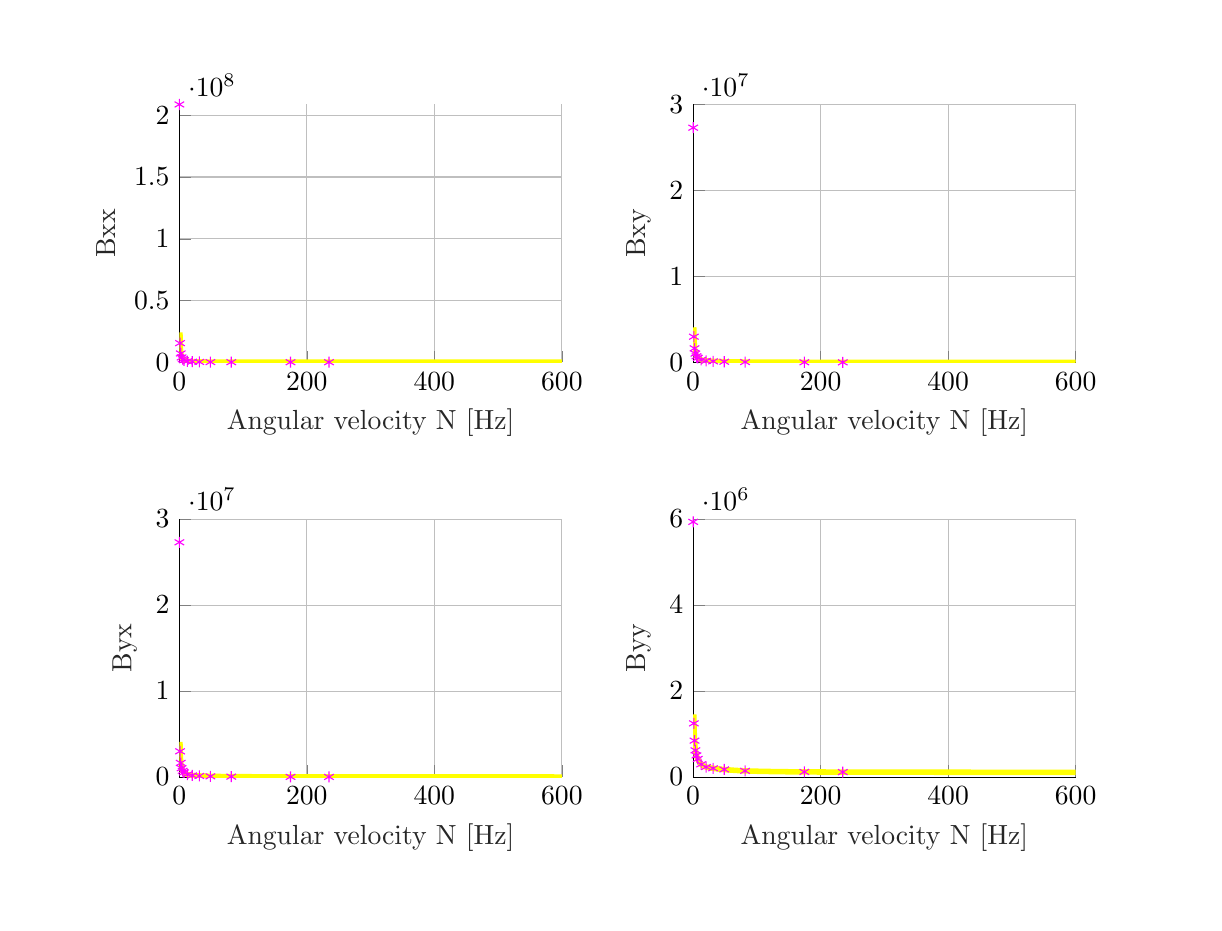
\begin{tikzpicture}

\begin{axis}[%
width=1.913in,
height=1.29in,
at={(0.758in,2.701in)},
scale only axis,
unbounded coords=jump,
xmin=0,
xmax=600,
xlabel style={font=\color{white!15!black}},
xlabel={Angular velocity N [Hz]},
ymin=0,
ymax=208702342.901601,
ylabel style={font=\color{white!15!black}},
ylabel={Bxx},
axis background/.style={fill=white},
axis x line*=bottom,
axis y line*=left,
xmajorgrids,
ymajorgrids
]
\addplot [color=mycolor1, only marks, mark=asterisk, mark options={solid, mycolor1}, forget plot]
  table[row sep=crcr]{%
234.77841101293	212179.047798931\\
174.508114226054	216193.855169977\\
81.5421662410681	251551.857748548\\
48.8465150429587	318696.352036701\\
31.4350959711944	426469.563344646\\
20.3658453848465	612401.746532875\\
12.7237293216739	980221.990580485\\
7.3663696072849	1819907.54839052\\
5.31796736354792	2634556.51017007\\
3.64773168788546	4101955.28295441\\
2.29263481895177	7285371.55025803\\
1.24085905149452	15644985.4385449\\
0.196567830697068	208702342.901601\\
};
\addplot [color=mycolor2, line width=2.0pt, forget plot]
  table[row sep=crcr]{%
0	inf\\
1.0016694490818	24322493.8666927\\
2.00333889816361	8709579.47343926\\
3.00500834724541	5253912.53260392\\
4.00667779632721	3683392.22679083\\
5.00834724540902	2832676.37422219\\
6.01001669449082	2297214.71942639\\
7.01168614357262	1926891.68993709\\
8.01335559265442	1658894.6173369\\
9.01502504173623	1455201.25414299\\
10.016694490818	1292246.56358786\\
11.0183639398998	1158919.99858821\\
12.0200333889816	1047814.52775517\\
13.0217028380634	957791.729576384\\
14.0233722871452	889378.034606642\\
15.025041736227	830086.165632866\\
16.0267111853088	778205.780280812\\
17.0283806343907	732428.969676059\\
18.0300500834725	691738.471360722\\
19.0317195325543	655331.183394368\\
20.0333889816361	622564.62422465\\
21.0350584307179	595603.195768336\\
22.0367278797997	572365.81475582\\
23.0383973288815	551149.07557048\\
24.0400667779633	531700.397983918\\
25.0417362270451	513807.614604281\\
26.0434056761269	497291.199176924\\
27.0450751252087	481998.221929371\\
28.0467445742905	467797.6001995\\
29.0484140233723	454576.331692379\\
30.0500834724541	442236.481085733\\
31.0517529215359	430692.749873064\\
32.0534223706177	420637.078455927\\
33.0550918196995	411651.693586803\\
34.0567612687813	403194.860768805\\
35.0584307178631	395221.275540406\\
36.0601001669449	387690.66726914\\
37.0617696160267	380567.11890443\\
38.0634390651085	373818.494137862\\
39.0651085141903	367415.952692656\\
40.0667779632721	361333.538319711\\
41.0684474123539	355547.82708691\\
42.0701168614357	350037.625912813\\
43.0717863105175	344783.713165418\\
44.0734557595993	339768.614633814\\
45.0751252086811	334976.409370282\\
46.0767946577629	330392.560857338\\
47.0784641068447	326003.769727923\\
48.0801335559265	321797.844895567\\
49.0818030050083	317893.599178851\\
50.0834724540901	314560.519219707\\
51.085141903172	311358.148278569\\
52.0868113522538	308278.945450552\\
53.0884808013356	305315.938955667\\
54.0901502504174	302462.673442075\\
55.0918196994992	299713.163038068\\
56.093489148581	297061.849434203\\
57.0951585976628	294503.564377843\\
58.0968280467446	292033.496047564\\
59.0984974958264	289647.158847125\\
60.1001669449082	287340.366220034\\
61.10183639399	285109.206138094\\
62.1035058430718	282950.018962022\\
63.1051752921536	280859.377410588\\
64.1068447412354	278834.068407636\\
65.1085141903172	276871.076604775\\
66.110183639399	274967.569402001\\
67.1118530884808	273120.883309757\\
68.1135225375626	271328.511514344\\
69.1151919866444	269588.092524595\\
70.1168614357262	267897.399791696\\
71.118530884808	266254.332206203\\
72.1202003338898	264656.905386973\\
73.1218697829716	263103.243686079\\
74.1235392320534	261591.572841965\\
75.1252086811352	260120.213220361\\
76.126878130217	258687.5735888\\
77.1285475792988	257292.145376239\\
78.1302170283806	255932.497374258\\
79.1318864774624	254607.270840681\\
80.1335559265442	253315.174970443\\
81.135225375626	252054.98270194\\
82.1368948247079	251071.284072747\\
83.1385642737897	250277.421516345\\
84.1402337228715	249502.46044938\\
85.1419031719533	248745.733760462\\
86.1435726210351	248006.605366634\\
87.1452420701169	247284.468430136\\
88.1469115191987	246578.743696741\\
89.1485809682805	245888.877946118\\
90.1502504173623	245214.342545509\\
91.1519198664441	244554.63209876\\
92.1535893155259	243909.263183461\\
93.1552587646077	243277.773169567\\
94.1569282136895	242659.719113416\\
95.1585976627713	242054.676721604\\
96.1602671118531	241462.239379622\\
97.1619365609349	240882.017240567\\
98.1636060100167	240313.636369657\\
99.1652754590985	239756.737940582\\
100.16694490818	239210.97748009\\
101.168614357262	238676.024157429\\
102.170283806344	238151.560115604\\
103.171953255426	237637.279841582\\
104.173622704508	237132.889572829\\
105.175292153589	236638.106737767\\
106.176961602671	236152.659427895\\
107.178631051753	235676.285899516\\
108.180300500835	235208.734103144\\
109.181969949917	234749.761238815\\
110.183639398998	234299.133335656\\
111.18530884808	233856.624854175\\
112.186978297162	233422.018309864\\
113.188647746244	232995.103916779\\
114.190317195326	232575.679249889\\
115.191986644407	232163.548925032\\
116.193656093489	231758.524295431\\
117.195325542571	231360.423163772\\
118.196994991653	230969.069508921\\
119.198664440735	230584.29322642\\
120.200333889816	230205.929881961\\
121.202003338898	229833.820477079\\
122.20367278798	229467.811226376\\
123.205342237062	229107.753345604\\
124.207011686144	228753.502850004\\
125.208681135225	228404.920362335\\
126.210350584307	228061.870930025\\
127.212020033389	227724.22385098\\
128.213689482471	227391.852507545\\
129.215358931553	227064.634208195\\
130.217028380634	226742.450036527\\
131.218697829716	226425.184707174\\
132.220367278798	226112.726428266\\
133.22203672788	225804.966770093\\
134.223706176962	225501.800539655\\
135.225375626043	225203.125660778\\
136.227045075125	224908.843059532\\
137.228714524207	224618.856554654\\
138.230383973289	224333.072752746\\
139.232053422371	224051.400947988\\
140.233722871452	223773.753026154\\
141.235392320534	223500.043372716\\
142.237061769616	223230.188784819\\
143.238731218698	222964.108386962\\
144.24040066778	222701.723550187\\
145.242070116861	222442.957814608\\
146.243739565943	222187.736815134\\
147.245409015025	221935.98821021\\
148.247078464107	221687.64161346\\
149.248747913189	221442.628528077\\
150.25041736227	221200.882283832\\
151.252086811352	220962.337976596\\
152.253756260434	220726.932410246\\
153.255425709516	220494.604040841\\
154.257095158598	220265.292922987\\
155.258764607679	220038.940658267\\
156.260434056761	219815.490345658\\
157.262103505843	219594.886533847\\
158.263772954925	219377.07517535\\
159.265442404007	219162.003582369\\
160.267111853088	218949.620384299\\
161.26878130217	218739.875486828\\
162.270450751252	218532.720032534\\
163.272120200334	218328.106362956\\
164.273789649416	218125.987982032\\
165.275459098497	217926.319520876\\
166.277128547579	217729.05670383\\
167.278797996661	217534.156315731\\
168.280467445743	217341.576170348\\
169.282136894825	217151.275079939\\
170.283806343907	216963.212825889\\
171.285475792988	216777.350130365\\
172.28714524207	216593.648628975\\
173.288814691152	216412.070844364\\
174.290484140234	216232.580160726\\
175.292153589316	216123.904008113\\
176.293823038397	216035.441342286\\
177.295492487479	215947.978254605\\
178.297161936561	215861.497898245\\
179.298831385643	215775.983802851\\
180.300500834725	215691.419864072\\
181.302170283806	215607.790333456\\
182.303839732888	215525.079808671\\
183.30550918197	215443.273224048\\
184.307178631052	215362.355841432\\
185.308848080134	215282.31324133\\
186.310517529215	215203.131314348\\
187.312186978297	215124.796252895\\
188.313856427379	215047.29454316\\
189.315525876461	214970.612957337\\
190.317195325543	214894.738546101\\
191.318864774624	214819.658631319\\
192.320534223706	214745.360798982\\
193.322203672788	214671.832892369\\
194.32387312187	214599.063005411\\
195.325542570952	214527.039476269\\
196.327212020033	214455.750881097\\
197.328881469115	214385.186028009\\
198.330550918197	214315.333951214\\
199.332220367279	214246.183905342\\
200.333889816361	214177.725359928\\
201.335559265442	214109.947994071\\
202.337228714524	214042.841691242\\
203.338898163606	213976.396534254\\
204.340567612688	213910.602800373\\
205.34223706177	213845.450956579\\
206.343906510851	213780.931654958\\
207.345575959933	213717.035728232\\
208.347245409015	213653.754185417\\
209.348914858097	213591.078207604\\
210.350584307179	213528.999143866\\
211.35225375626	213467.508507273\\
212.353923205342	213406.597971025\\
213.355592654424	213346.259364694\\
214.357262103506	213286.484670572\\
215.358931552588	213227.266020117\\
216.360601001669	213168.595690499\\
217.362270450751	213110.466101246\\
218.363939899833	213052.869810977\\
219.365609348915	212995.799514227\\
220.367278797997	212939.248038356\\
221.368948247078	212883.208340547\\
222.37061769616	212827.673504881\\
223.372287145242	212772.63673949\\
224.373956594324	212718.091373789\\
225.375626043406	212664.030855784\\
226.377295492487	212610.448749443\\
227.378964941569	212557.338732144\\
228.380634390651	212504.69459219\\
229.382303839733	212452.510226384\\
230.383973288815	212400.779637672\\
231.385642737896	212349.496932845\\
232.387312186978	212298.656320301\\
233.38898163606	212248.252107865\\
234.390651085142	212198.278700663\\
235.392320534224	212148.730599055\\
236.393989983306	212099.602396612\\
237.395659432387	212050.888778157\\
238.397328881469	212002.584517839\\
239.398998330551	211954.684477273\\
240.400667779633	211907.183603712\\
241.402337228715	211860.076928272\\
242.404006677796	211813.359564199\\
243.405676126878	211767.026705181\\
244.40734557596	211721.073623695\\
245.409015025042	211675.495669405\\
246.410684474124	211630.288267589\\
247.412353923205	211585.446917609\\
248.414023372287	211540.96719142\\
249.415692821369	211496.844732107\\
250.417362270451	211453.075252469\\
251.419031719533	211409.654533625\\
252.420701168614	211366.578423661\\
253.422370617696	211323.842836305\\
254.424040066778	211281.443749637\\
255.42570951586	211239.377204825\\
256.427378964942	211197.639304895\\
257.429048414023	211156.226213524\\
258.430717863105	211115.13415387\\
259.432387312187	211074.359407417\\
260.434056761269	211033.89831286\\
261.435726210351	210993.747265005\\
262.437395659432	210953.902713698\\
263.439065108514	210914.361162782\\
264.440734557596	210875.119169069\\
265.442404006678	210836.173341347\\
266.44407345576	210797.520339397\\
267.445742904841	210759.156873042\\
268.447412353923	210721.079701212\\
269.449081803005	210683.285631031\\
270.450751252087	210645.771516926\\
271.452420701169	210608.534259752\\
272.45409015025	210571.570805939\\
273.455759599332	210534.878146659\\
274.457429048414	210498.453317009\\
275.459098497496	210462.293395212\\
276.460767946578	210426.395501833\\
277.462437395659	210390.75679902\\
278.464106844741	210355.374489752\\
279.465776293823	210320.24581711\\
280.467445742905	210285.368063558\\
281.469115191987	210250.738550246\\
282.470784641068	210216.354636318\\
283.47245409015	210182.213718248\\
284.474123539232	210148.313229179\\
285.475792988314	210114.650638279\\
286.477462437396	210081.223450113\\
287.479131886477	210048.029204024\\
288.480801335559	210015.065473533\\
289.482470784641	209982.329865744\\
290.484140233723	209949.820020768\\
291.485809682805	209917.533611152\\
292.487479131886	209885.468341329\\
293.489148580968	209853.621947067\\
294.49081803005	209821.992194943\\
295.492487479132	209790.576881817\\
296.494156928214	209759.373834319\\
297.495826377295	209728.380908354\\
298.497495826377	209697.595988603\\
299.499165275459	209667.016988048\\
300.500834724541	209636.641847497\\
301.502504173623	209606.468535122\\
302.504173622705	209576.495046008\\
303.505843071786	209546.719401706\\
304.507512520868	209517.139649801\\
305.50918196995	209487.753863483\\
306.510851419032	209458.560141127\\
307.512520868114	209429.556605888\\
308.514190317195	209400.741405293\\
309.515859766277	209372.11271085\\
310.517529215359	209343.668717663\\
311.519198664441	209315.407644045\\
312.520868113523	209287.327731156\\
313.522537562604	209259.42724263\\
314.524207011686	209231.704464223\\
315.525876460768	209204.157703456\\
316.52754590985	209176.785289276\\
317.529215358932	209149.585571716\\
318.530884808013	209122.556921561\\
319.532554257095	209095.697730029\\
320.534223706177	209069.006408443\\
321.535893155259	209042.481387927\\
322.537562604341	209016.12111909\\
323.539232053422	208989.924071733\\
324.540901502504	208963.888734544\\
325.542570951586	208938.013614815\\
326.544240400668	208912.297238152\\
327.54590984975	208886.738148196\\
328.547579298831	208861.33490635\\
329.549248747913	208836.086091506\\
330.550918196995	208810.990299782\\
331.552587646077	208786.046144262\\
332.554257095159	208761.252254739\\
333.55592654424	208736.607277466\\
334.557595993322	208712.109874906\\
335.559265442404	208687.758725496\\
336.560934891486	208663.552523405\\
337.562604340568	208639.489978298\\
338.564273789649	208615.569815116\\
339.565943238731	208591.79077384\\
340.567612687813	208568.151609278\\
341.569282136895	208544.651090842\\
342.570951585977	208521.288002338\\
343.572621035058	208498.061141756\\
344.57429048414	208474.969321061\\
345.575959933222	208452.011365993\\
346.577629382304	208429.186115868\\
347.579298831386	208406.49242338\\
348.580968280467	208383.929154412\\
349.582637729549	208361.495187846\\
350.584307178631	208339.189415374\\
351.585976627713	208317.01074132\\
352.587646076795	208294.95808246\\
353.589315525876	208273.030367843\\
354.590984974958	208251.22653862\\
355.59265442404	208229.54554787\\
356.594323873122	208207.98636044\\
357.595993322204	208186.547952771\\
358.597662771285	208165.229312743\\
359.599332220367	208144.029439511\\
360.601001669449	208122.947343353\\
361.602671118531	208101.982045512\\
362.604340567613	208081.132578045\\
363.606010016694	208060.397983678\\
364.607679465776	208039.777315653\\
365.609348914858	208019.26963759\\
366.61101836394	207998.874023341\\
367.612687813022	207978.589556854\\
368.614357262104	207958.415332033\\
369.616026711185	207938.350452604\\
370.617696160267	207918.394031982\\
371.619365609349	207898.545193143\\
372.621035058431	207878.803068491\\
373.622704507513	207859.166799736\\
374.624373956594	207839.635537765\\
375.626043405676	207820.208442524\\
376.627712854758	207800.884682897\\
377.62938230384	207781.663436583\\
378.631051752922	207762.543889986\\
379.632721202003	207743.525238093\\
380.634390651085	207724.606684368\\
381.636060100167	207705.787440636\\
382.637729549249	207687.066726977\\
383.639398998331	207668.443771613\\
384.641068447412	207649.917810808\\
385.642737896494	207631.488088761\\
386.644407345576	207613.153857502\\
387.646076794658	207594.914376791\\
388.64774624374	207576.768914023\\
389.649415692821	207558.716744122\\
390.651085141903	207540.757149452\\
391.652754590985	207522.889419716\\
392.654424040067	207505.112851866\\
393.656093489149	207487.42675001\\
394.65776293823	207469.830425322\\
395.659432387312	207452.323195948\\
396.661101836394	207434.904386924\\
397.662771285476	207417.573330087\\
398.664440734558	207400.329363988\\
399.666110183639	207383.171833809\\
400.667779632721	207366.100091281\\
401.669449081803	207349.113494601\\
402.671118530885	207332.211408353\\
403.672787979967	207315.393203425\\
404.674457429048	207298.658256938\\
405.67612687813	207282.005952162\\
406.677796327212	207265.435678444\\
407.679465776294	207248.946831133\\
408.681135225376	207232.538811504\\
409.682804674457	207216.21102669\\
410.684474123539	207199.962889607\\
411.686143572621	207183.793818885\\
412.687813021703	207167.703238797\\
413.689482470785	207151.690579193\\
414.691151919866	207135.755275433\\
415.692821368948	207119.896768318\\
416.69449081803	207104.114504026\\
417.696160267112	207088.407934046\\
418.697829716194	207072.77651512\\
419.699499165275	207057.219709171\\
420.701168614357	207041.736983251\\
421.702838063439	207026.327809472\\
422.704507512521	207010.991664954\\
423.706176961603	206995.728031757\\
424.707846410684	206980.53639683\\
425.709515859766	206965.416251949\\
426.711185308848	206950.367093664\\
427.71285475793	206935.38842324\\
428.714524207012	206920.479746604\\
429.716193656093	206905.640574287\\
430.717863105175	206890.870421376\\
431.719532554257	206876.168807458\\
432.721202003339	206861.535256567\\
433.722871452421	206846.969297135\\
434.724540901503	206832.47046194\\
435.726210350584	206818.038288057\\
436.727879799666	206803.672316806\\
437.729549248748	206789.372093707\\
438.73121869783	206775.137168431\\
439.732888146912	206760.96709475\\
440.734557595993	206746.861430495\\
441.736227045075	206732.819737507\\
442.737896494157	206718.841581591\\
443.739565943239	206704.926532474\\
444.741235392321	206691.074163758\\
445.742904841402	206677.284052879\\
446.744574290484	206663.555781062\\
447.746243739566	206649.88893328\\
448.747913188648	206636.283098212\\
449.74958263773	206622.7378682\\
450.751252086811	206609.25283921\\
451.752921535893	206595.827610791\\
452.754590984975	206582.461786039\\
453.756260434057	206569.15497155\\
454.757929883139	206555.906777389\\
455.75959933222	206542.716817049\\
456.761268781302	206529.584707412\\
457.762938230384	206516.510068715\\
458.764607679466	206503.49252451\\
459.766277128548	206490.53170163\\
460.767946577629	206477.627230154\\
461.769616026711	206464.778743369\\
462.771285475793	206451.98587774\\
463.772954924875	206439.248272869\\
464.774624373957	206426.565571468\\
465.776293823038	206413.93741932\\
466.77796327212	206401.36346525\\
467.779632721202	206388.84336109\\
468.781302170284	206376.376761649\\
469.782971619366	206363.963324679\\
470.784641068447	206351.602710845\\
471.786310517529	206339.294583693\\
472.787979966611	206327.038609623\\
473.789649415693	206314.834457854\\
474.791318864775	206302.681800396\\
475.792988313856	206290.580312021\\
476.794657762938	206278.529670237\\
477.79632721202	206266.529555252\\
478.797996661102	206254.579649954\\
479.799666110184	206242.679639876\\
480.801335559265	206230.829213174\\
481.803005008347	206219.028060594\\
482.804674457429	206207.275875454\\
483.806343906511	206195.572353605\\
484.808013355593	206183.917193417\\
485.809682804674	206172.310095745\\
486.811352253756	206160.750763908\\
487.813021702838	206149.238903659\\
488.81469115192	206137.774223165\\
489.816360601002	206126.35643298\\
490.818030050083	206114.98524602\\
491.819699499165	206103.66037754\\
492.821368948247	206092.381545112\\
493.823038397329	206081.148468595\\
494.824707846411	206069.960870122\\
495.826377295492	206058.818474066\\
496.828046744574	206047.721007027\\
497.829716193656	206036.668197803\\
498.831385642738	206025.659777371\\
499.83305509182	206014.695478864\\
500.834724540902	206003.775037552\\
501.836393989983	205992.898190816\\
502.838063439065	205982.06467813\\
503.839732888147	205971.274241042\\
504.841402337229	205960.526623148\\
505.843071786311	205949.821570078\\
506.844741235392	205939.15882947\\
507.846410684474	205928.538150955\\
508.848080133556	205917.959286136\\
509.849749582638	205907.421988565\\
510.85141903172	205896.92601373\\
511.853088480801	205886.471119031\\
512.854757929883	205876.057063765\\
513.856427378965	205865.683609104\\
514.858096828047	205855.35051808\\
515.859766277129	205845.057555564\\
516.86143572621	205834.804488252\\
517.863105175292	205824.591084644\\
518.864774624374	205814.417115026\\
519.866444073456	205804.282351457\\
520.868113522538	205794.186567747\\
521.869782971619	205784.129539446\\
522.871452420701	205774.11104382\\
523.873121869783	205764.130859841\\
524.874791318865	205754.188768166\\
525.876460767947	205744.284551127\\
526.878130217028	205734.417992708\\
527.87979966611	205724.588878533\\
528.881469115192	205714.796995852\\
529.883138564274	205705.042133521\\
530.884808013356	205695.324081991\\
531.886477462437	205685.642633291\\
532.888146911519	205675.997581016\\
533.889816360601	205666.388720306\\
534.891485809683	205656.815847838\\
535.893155258765	205647.27876181\\
536.894824707846	205637.777261923\\
537.896494156928	205628.311149373\\
538.89816360601	205618.880226833\\
539.899833055092	205609.484298439\\
540.901502504174	205600.12316978\\
541.903171953255	205590.796647882\\
542.904841402337	205581.504541193\\
543.906510851419	205572.246659575\\
544.908180300501	205563.022814287\\
545.909849749583	205553.832817972\\
546.911519198664	205544.676484647\\
547.913188647746	205535.553629689\\
548.914858096828	205526.464069822\\
549.91652754591	205517.407623106\\
550.918196994992	205508.384108923\\
551.919866444073	205499.393347968\\
552.921535893155	205490.435162234\\
553.923205342237	205481.509375001\\
554.924874791319	205472.615810827\\
555.926544240401	205463.754295533\\
556.928213689483	205454.924656193\\
557.929883138564	205446.126721124\\
558.931552587646	205437.360319872\\
559.933222036728	205428.625283205\\
560.93489148581	205419.921443097\\
561.936560934892	205411.248632721\\
562.938230383973	205402.60668644\\
563.939899833055	205393.99543979\\
564.941569282137	205385.414729476\\
565.943238731219	205376.864393358\\
566.9449081803	205368.344270442\\
567.946577629382	205359.854200869\\
568.948247078464	205351.394025907\\
569.949916527546	205342.96358794\\
570.951585976628	205334.562730457\\
571.953255425709	205326.191298044\\
572.954924874791	205317.849136374\\
573.956594323873	205309.536092196\\
574.958263772955	205301.252013329\\
575.959933222037	205292.99674865\\
576.961602671118	205284.770148084\\
577.9632721202	205276.572062598\\
578.964941569282	205268.402344189\\
579.966611018364	205260.260845879\\
580.968280467446	205252.147421701\\
581.969949916528	205244.061926694\\
582.971619365609	205236.004216893\\
583.973288814691	205227.974149322\\
584.974958263773	205219.971581982\\
585.976627712855	205211.996373846\\
586.978297161937	205204.048384851\\
587.979966611018	205196.127475886\\
588.9816360601	205188.233508789\\
589.983305509182	205180.366346334\\
590.984974958264	205172.525852226\\
591.986644407346	205164.711891093\\
592.988313856427	205156.924328477\\
593.989983305509	205149.163030828\\
594.991652754591	205141.427865494\\
595.993322203673	205133.718700716\\
596.994991652755	205126.035405619\\
597.996661101836	205118.377850204\\
598.998330550918	205110.745905341\\
600	205103.139442766\\
};
\end{axis}

\begin{axis}[%
width=1.913in,
height=1.29in,
at={(3.327in,2.701in)},
scale only axis,
unbounded coords=jump,
xmin=0,
xmax=600,
xlabel style={font=\color{white!15!black}},
xlabel={Angular velocity N [Hz]},
ymin=0,
ymax=30000000,
ylabel style={font=\color{white!15!black}},
ylabel={Bxy},
axis background/.style={fill=white},
axis x line*=bottom,
axis y line*=left,
xmajorgrids,
ymajorgrids
]
\addplot [color=mycolor1, only marks, mark=asterisk, mark options={solid, mycolor1}, forget plot]
  table[row sep=crcr]{%
234.77841101293	16069.4425906544\\
174.508114226054	21829.2824637647\\
81.5421662410681	49861.1718037301\\
48.8465150429587	86985.357261782\\
31.4350959711944	130504.347253006\\
20.3658453848465	188846.353556393\\
12.7237293216739	299392.326051015\\
7.3663696072849	537021.899525072\\
5.31796736354792	723211.591027077\\
3.64773168788546	1029254.38556384\\
2.29263481895177	1645599.27560653\\
1.24085905149452	2996162.3056836\\
0.196567830697068	27299011.8170398\\
};
\addplot [color=mycolor2, line width=2.0pt, forget plot]
  table[row sep=crcr]{%
0	inf\\
1.0016694490818	4088522.54636056\\
2.00333889816361	1875691.54947177\\
3.00500834724541	1252286.15544622\\
4.00667779632721	941958.273713417\\
5.00834724540902	764531.754279433\\
6.01001669449082	646111.432681455\\
7.01168614357262	561473.344558096\\
8.01335559265442	491455.516044728\\
9.01502504173623	433810.643431334\\
10.016694490818	387694.745340619\\
11.0183639398998	349963.555993671\\
12.0200333889816	318520.898204547\\
13.0217028380634	292651.057575086\\
14.0233722871452	272089.768291069\\
15.025041736227	254269.984244922\\
16.0267111853088	238677.673204542\\
17.0283806343907	224919.751698326\\
18.0300500834725	212690.488137244\\
19.0317195325543	201748.515477329\\
20.0333889816361	191900.740083405\\
21.0350584307179	183575.285698279\\
22.0367278797997	176283.834555935\\
23.0383973288815	169626.422643359\\
24.0400667779633	163523.795056832\\
25.0417362270451	157909.377677227\\
26.0434056761269	152726.838557591\\
27.0450751252087	147928.191224596\\
28.0467445742905	143472.304415385\\
29.0484140233723	139323.720144741\\
30.0500834724541	135451.708158806\\
31.0517529215359	131829.503397771\\
32.0534223706177	128149.180802868\\
33.0550918196995	124520.868447311\\
34.0567612687813	121105.986230316\\
35.0584307178631	117886.240140006\\
36.0601001669449	114845.368832492\\
37.0617696160267	111968.868947005\\
38.0634390651085	109243.763792333\\
39.0651085141903	106658.407619953\\
40.0667779632721	104202.319256191\\
41.0684474123539	101866.040080905\\
42.0701168614357	99641.012294919\\
43.0717863105175	97519.4741733971\\
44.0734557595993	95494.3696028536\\
45.0751252086811	93559.2696798898\\
46.0767946577629	91708.3045361852\\
47.0784641068447	89936.1038666809\\
48.0801335559265	88237.7448917392\\
49.0818030050083	86541.5152716416\\
50.0834724540901	84698.6556319705\\
51.085141903172	82928.0649977768\\
52.0868113522538	81225.5740033596\\
53.0884808013356	79587.327952128\\
54.0901502504174	78009.7576805717\\
55.0918196994992	76489.5536007084\\
56.093489148581	75023.6425236972\\
57.0951585976628	73609.1669230725\\
58.0968280467446	72243.4663431589\\
59.0984974958264	70924.0606981577\\
60.1001669449082	69648.6352413232\\
61.10183639399	68415.0270125816\\
62.1035058430718	67221.2125976704\\
63.1051752921536	66065.2970530738\\
64.1068447412354	64945.5038692459\\
65.1085141903172	63860.165860305\\
66.110183639399	62807.716881938\\
67.1118530884808	61786.684290985\\
68.1135225375626	60795.6820703541\\
69.1151919866444	59833.4045517706\\
70.1168614357262	58898.6206765751\\
71.118530884808	57990.1687415259\\
72.1202003338898	57106.9515824504\\
73.1218697829716	56247.9321537605\\
74.1235392320534	55412.1294663865\\
75.1252086811352	54598.6148506758\\
76.126878130217	53806.508514326\\
77.1285475792988	53034.9763685306\\
78.1302170283806	52283.2270982685\\
79.1318864774624	51550.5094551017\\
80.1335559265442	50836.109753014\\
81.135225375626	50139.3495497433\\
82.1368948247079	49480.1721115157\\
83.1385642737897	48850.7964197533\\
84.1402337228715	48236.405863509\\
85.1419031719533	47636.471555647\\
86.1435726210351	47050.4892084329\\
87.1452420701169	46477.9777197754\\
88.1469115191987	45918.4778558602\\
89.1485809682805	45371.5510225948\\
90.1502504173623	44836.7781189575\\
91.1519198664441	44313.7584659495\\
92.1535893155259	43802.1088053983\\
93.1552587646077	43301.4623633535\\
94.1569282136895	42811.4679732672\\
95.1585976627713	42331.7892545511\\
96.1602671118531	41862.1038424749\\
97.1619365609349	41402.1026656992\\
98.1636060100167	40951.4892680414\\
99.1652754590985	40509.9791713464\\
100.16694490818	40077.2992765853\\
101.168614357262	39653.1873005323\\
102.170283806344	39237.3912455784\\
103.171953255426	38829.6689004295\\
104.173622704508	38429.7873696103\\
105.175292153589	38037.5226298544\\
106.176961602671	37652.6591116032\\
107.178631051753	37274.9893039736\\
108.180300500835	36904.3133816705\\
109.181969949917	36540.4388524372\\
110.183639398998	36183.1802237353\\
111.18530884808	35832.3586874425\\
112.186978297162	35487.8018214407\\
113.188647746244	35149.3433070495\\
114.190317195326	34816.8226613318\\
115.191986644407	34490.0849833658\\
116.193656093489	34168.9807136405\\
117.195325542571	33853.3654057909\\
118.196994991653	33543.0995099387\\
119.198664440735	33238.048166958\\
120.200333889816	32938.081013027\\
121.202003338898	32643.0719938717\\
122.20367278798	32352.8991881452\\
123.205342237062	32067.4446394224\\
124.207011686144	31786.5941963241\\
125.208681135225	31510.2373603154\\
126.210350584307	31238.2671407513\\
127.212020033389	30970.5799167708\\
128.213689482471	30707.0753056651\\
129.215358931553	30447.6560373672\\
130.217028380634	30192.2278347354\\
131.218697829716	29940.6992993194\\
132.220367278798	29692.9818023187\\
133.22203672788	29448.989380461\\
134.223706176962	29208.6386365414\\
135.225375626043	28971.8486443835\\
136.227045075125	28738.5408579928\\
137.228714524207	28508.639024688\\
138.230383973289	28282.0691020108\\
139.232053422371	28058.759178221\\
140.233722871452	27838.6393961997\\
141.235392320534	27621.64188059\\
142.237061769616	27407.7006680171\\
143.238731218698	27196.7516402354\\
144.24040066778	26988.7324600618\\
145.242070116861	26783.5825099596\\
146.243739565943	26581.2428331464\\
147.245409015025	26381.6560771062\\
148.247078464107	26184.7664393908\\
149.248747913189	25990.5196156046\\
150.25041736227	25798.8627494688\\
151.252086811352	25609.7443848712\\
152.253756260434	25423.1144198078\\
153.255425709516	25238.9240621309\\
154.257095158598	25057.1257870212\\
155.258764607679	24877.6732961064\\
156.260434056761	24700.5214781521\\
157.262103505843	24525.6263712546\\
158.263772954925	24352.9451264696\\
159.265442404007	24182.4359728141\\
160.267111853088	24014.0581835792\\
161.26878130217	23847.7720439001\\
162.270450751252	23683.5388195256\\
163.272120200334	23521.3207267385\\
164.273789649416	23361.0809033757\\
165.275459098497	23202.7833809021\\
166.277128547579	23046.3930574945\\
167.278797996661	22891.8756720918\\
168.280467445743	22739.1977793724\\
169.282136894825	22588.3267256201\\
170.283806343907	22439.2306254414\\
171.285475792988	22291.8783392998\\
172.28714524207	22146.2394518343\\
173.288814691152	22002.2842509291\\
174.290484140234	21859.9837075056\\
175.292153589316	21728.9270907562\\
176.293823038397	21602.0142048269\\
177.295492487479	21476.5353628065\\
178.297161936561	21352.4663954155\\
179.298831385643	21229.7836734701\\
180.300500834725	21108.4640928798\\
181.302170283806	20988.4850601412\\
182.303839732888	20869.8244783119\\
183.30550918197	20752.4607334425\\
184.307178631052	20636.372681452\\
185.308848080134	20521.5396354291\\
186.310517529215	20407.9413533418\\
187.312186978297	20295.5580261433\\
188.313856427379	20184.3702662553\\
189.315525876461	20074.359096419\\
190.317195325543	19965.5059388968\\
191.318864774624	19857.7926050136\\
192.320534223706	19751.2012850251\\
193.322203672788	19645.7145383006\\
194.32387312187	19541.3152838104\\
195.325542570952	19437.9867909047\\
196.327212020033	19335.7126703756\\
197.328881469115	19234.476865791\\
198.330550918197	19134.2636450911\\
199.332220367279	19035.0575924384\\
200.333889816361	18936.8436003122\\
201.335559265442	18839.606861839\\
202.337228714524	18743.3328633507\\
203.338898163606	18648.0073771628\\
204.340567612688	18553.616454565\\
205.34223706177	18460.1464190169\\
206.343906510851	18367.5838595421\\
207.345575959933	18275.9156243134\\
208.347245409015	18185.1288144234\\
209.348914858097	18095.2107778339\\
210.350584307179	18006.1491034975\\
211.35225375626	17917.9316156478\\
212.353923205342	17830.5463682495\\
213.355592654424	17743.9816396061\\
214.357262103506	17658.2259271182\\
215.358931552588	17573.2679421884\\
216.360601001669	17489.0966052672\\
217.362270450751	17405.7010410365\\
218.363939899833	17323.0705737253\\
219.365609348915	17241.194722554\\
220.367278797997	17160.0631973024\\
221.368948247078	17079.6658939988\\
222.37061769616	16999.9928907249\\
223.372287145242	16921.0344435342\\
224.373956594324	16842.7809824792\\
225.375626043406	16765.2231077446\\
226.377295492487	16688.3515858838\\
227.378964941569	16612.157346154\\
228.380634390651	16536.6314769481\\
229.382303839733	16461.7652223204\\
230.383973288815	16387.5499786025\\
231.385642737896	16313.9772911072\\
232.387312186978	16241.038850918\\
233.38898163606	16168.7264917604\\
234.390651085142	16097.0321869546\\
235.392320534224	16025.948046445\\
236.393989983306	15955.4663139059\\
237.395659432387	15885.5793639198\\
238.397328881469	15816.2796992277\\
239.398998330551	15747.5599480477\\
240.400667779633	15679.4128614609\\
241.402337228715	15611.8313108623\\
242.404006677796	15544.8082854753\\
243.405676126878	15478.3368899268\\
244.40734557596	15412.4103418829\\
245.409015025042	15347.0219697413\\
246.410684474124	15282.1652103814\\
247.412353923205	15217.8336069678\\
248.414023372287	15154.0208068074\\
249.415692821369	15090.7205592588\\
250.417362270451	15027.9267136906\\
251.419031719533	14965.6332174895\\
252.420701168614	14903.8341141153\\
253.422370617696	14842.5235412026\\
254.424040066778	14781.6957287066\\
255.42570951586	14721.3449970928\\
256.427378964942	14661.4657555698\\
257.429048414023	14602.0525003622\\
258.430717863105	14543.0998130243\\
259.432387312187	14484.6023587934\\
260.434056761269	14426.5548849796\\
261.435726210351	14368.9522193942\\
262.437395659432	14311.7892688134\\
263.439065108514	14255.0610174764\\
264.440734557596	14198.7625256193\\
265.442404006678	14142.8889280404\\
266.44407345576	14087.4354326989\\
267.445742904841	14032.397319345\\
268.447412353923	13977.7699381803\\
269.449081803005	13923.5487085484\\
270.450751252087	13869.7291176546\\
271.452420701169	13816.3067193134\\
272.45409015025	13763.2771327248\\
273.455759599332	13710.636041276\\
274.457429048414	13658.3791913706\\
275.459098497496	13606.5023912827\\
276.460767946578	13555.0015100361\\
277.462437395659	13503.8724763074\\
278.464106844741	13453.1112773538\\
279.465776293823	13402.7139579626\\
280.467445742905	13352.6766194242\\
281.469115191987	13302.9954185266\\
282.470784641068	13253.6665665716\\
283.47245409015	13204.6863284113\\
284.474123539232	13156.0510215056\\
285.475792988314	13107.7570149993\\
286.477462437396	13059.8007288182\\
287.479131886477	13012.1786327847\\
288.480801335559	12964.8872457514\\
289.482470784641	12917.923134753\\
290.484140233723	12871.2829141752\\
291.485809682805	12824.9632449416\\
292.487479131886	12778.9608337165\\
293.489148580968	12733.2724321243\\
294.49081803005	12687.8948359851\\
295.492487479132	12642.8248845655\\
296.494156928214	12598.0594598447\\
297.495826377295	12553.5954857954\\
298.497495826377	12509.4299276793\\
299.499165275459	12465.5597913567\\
300.500834724541	12421.9821226095\\
301.502504173623	12378.6940064786\\
302.504173622705	12335.6925666135\\
303.505843071786	12292.9749646352\\
304.507512520868	12250.5383995121\\
305.50918196995	12208.3801069471\\
306.510851419032	12166.497358778\\
307.512520868114	12124.8874623885\\
308.514190317195	12083.5477601315\\
309.515859766277	12042.4756287628\\
310.517529215359	12001.6684788868\\
311.519198664441	11961.1237544119\\
312.520868113523	11920.838932017\\
313.522537562604	11880.8115206278\\
314.524207011686	11841.0390609035\\
315.525876460768	11801.5191247331\\
316.52754590985	11762.2493147409\\
317.529215358932	11723.2272638023\\
318.530884808013	11684.4506345677\\
319.532554257095	11645.917118996\\
320.534223706177	11607.6244378967\\
321.535893155259	11569.5703404802\\
322.537562604341	11531.7526039172\\
323.539232053422	11494.1690329057\\
324.540901502504	11456.8174592462\\
325.542570951586	11419.6957414245\\
326.544240400668	11382.8017642029\\
327.54590984975	11346.1334382182\\
328.547579298831	11309.6886995871\\
329.549248747913	11273.4655095191\\
330.550918196995	11237.4618539363\\
331.552587646077	11201.6757431002\\
332.554257095159	11166.1052112451\\
333.55592654424	11130.748316218\\
334.557595993322	11095.6031391251\\
335.559265442404	11060.6677839851\\
336.560934891486	11025.9403773875\\
337.562604340568	10991.4190681585\\
338.564273789649	10957.1020270314\\
339.565943238731	10922.9874463239\\
340.567612687813	10889.0735396206\\
341.569282136895	10855.3585414611\\
342.570951585977	10821.8407070334\\
343.572621035058	10788.5183118736\\
344.57429048414	10755.3896515693\\
345.575959933222	10722.4530414697\\
346.577629382304	10689.7068163996\\
347.579298831386	10657.1493303788\\
348.580968280467	10624.7789563467\\
349.582637729549	10592.5940858907\\
350.584307178631	10560.5931289802\\
351.585976627713	10528.7745137045\\
352.587646076795	10497.1366860155\\
353.589315525876	10465.678109475\\
354.590984974958	10434.3972650053\\
355.59265442404	10403.2926506453\\
356.594323873122	10372.3627813098\\
357.595993322204	10341.6061885532\\
358.597662771285	10311.0214203371\\
359.599332220367	10280.6070408019\\
360.601001669449	10250.361630042\\
361.602671118531	10220.2837838845\\
362.604340567613	10190.3721136727\\
363.606010016694	10160.6252460516\\
364.607679465776	10131.041822758\\
365.609348914858	10101.620500414\\
366.61101836394	10072.3599503233\\
367.612687813022	10043.2588582712\\
368.614357262104	10014.3159243281\\
369.616026711185	9985.52986265567\\
370.617696160267	9956.89940131661\\
371.619365609349	9928.42328208719\\
372.621035058431	9900.10026027299\\
373.622704507513	9871.9291045275\\
374.624373956594	9843.9085966737\\
375.626043405676	9816.03753152844\\
376.627712854758	9788.31471672971\\
377.62938230384	9760.73897256651\\
378.631051752922	9733.30913181158\\
379.632721202003	9706.02403955668\\
380.634390651085	9678.88255305049\\
381.636060100167	9651.88354153908\\
382.637729549249	9625.02588610888\\
383.639398998331	9598.30847953212\\
384.641068447412	9571.73022611459\\
385.642737896494	9545.29004154599\\
386.644407345576	9518.98685275236\\
387.646076794658	9492.81959775094\\
388.64774624374	9466.78722550727\\
389.649415692821	9440.88869579441\\
390.651085141903	9415.12297905443\\
391.652754590985	9389.48905626197\\
392.654424040067	9363.98591878989\\
393.656093489149	9338.61256827695\\
394.65776293823	9313.36801649757\\
395.659432387312	9288.25128523354\\
396.661101836394	9263.26140614761\\
397.662771285476	9238.39742065909\\
398.664440734558	9213.65837982126\\
399.666110183639	9189.04334420067\\
400.667779632721	9164.55138375817\\
401.669449081803	9140.18157773185\\
402.671118530885	9115.93301452158\\
403.672787979967	9091.80479157539\\
404.674457429048	9067.79601527744\\
405.67612687813	9043.90580083775\\
406.677796327212	9020.13327218348\\
407.679465776294	8996.47756185184\\
408.681135225376	8972.93781088457\\
409.682804674457	8949.51316872398\\
410.684474123539	8926.20279311052\\
411.686143572621	8903.00584998179\\
412.687813021703	8879.9215133731\\
413.689482470785	8856.94896531943\\
414.691151919866	8834.08739575876\\
415.692821368948	8811.33600243694\\
416.69449081803	8788.69399081379\\
417.696160267112	8766.1605739706\\
418.697829716194	8743.734972519\\
419.699499165275	8721.41641451109\\
420.701168614357	8699.20413535084\\
421.702838063439	8677.09737770678\\
422.704507512521	8655.09539142598\\
423.706176961603	8633.19743344909\\
424.707846410684	8611.40276772682\\
425.709515859766	8589.71066513735\\
426.711185308848	8568.12040340511\\
427.71285475793	8546.63126702056\\
428.714524207012	8525.24254716118\\
429.716193656093	8503.95354161349\\
430.717863105175	8482.76355469626\\
431.719532554257	8461.67189718468\\
432.721202003339	8440.67788623565\\
433.722871452421	8419.7808453141\\
434.724540901503	8398.9801041203\\
435.726210350584	8378.27499851819\\
436.727879799666	8357.66487046472\\
437.729549248748	8337.14906794009\\
438.73121869783	8316.72694487905\\
439.732888146912	8296.39786110303\\
440.734557595993	8276.16118225326\\
441.736227045075	8256.01627972481\\
442.737896494157	8235.96253060146\\
443.739565943239	8215.99931759153\\
444.741235392321	8196.12602896453\\
445.742904841402	8176.34205848866\\
446.744574290484	8156.64680536919\\
447.746243739566	8137.03967418761\\
448.747913188648	8117.52007484167\\
449.74958263773	8098.08742248613\\
450.751252086811	8078.74113747439\\
451.752921535893	8059.48064530085\\
452.754590984975	8040.30537654399\\
453.756260434057	8021.21476681035\\
454.757929883139	8002.20825667906\\
455.75959933222	7983.28529164724\\
456.761268781302	7964.44532207609\\
457.762938230384	7945.68780313765\\
458.764607679466	7927.01219476224\\
459.766277128548	7908.41796158674\\
460.767946577629	7889.9045729033\\
461.769616026711	7871.47150260894\\
462.771285475793	7853.11822915569\\
463.772954924875	7834.84423550136\\
464.774624373957	7816.64900906107\\
465.776293823038	7798.53204165922\\
466.77796327212	7780.49282948228\\
467.779632721202	7762.530873032\\
468.781302170284	7744.64567707938\\
469.782971619366	7726.8367506191\\
470.784641068447	7709.10360682459\\
471.786310517529	7691.44576300375\\
472.787979966611	7673.86274055502\\
473.789649415693	7656.35406492425\\
474.791318864775	7638.91926556197\\
475.792988313856	7621.55787588121\\
476.794657762938	7604.26943321593\\
477.79632721202	7587.05347877985\\
478.797996661102	7569.90955762593\\
479.799666110184	7552.83721860626\\
480.801335559265	7535.8360143325\\
481.803005008347	7518.90550113681\\
482.804674457429	7502.04523903321\\
483.806343906511	7485.25479167953\\
484.808013355593	7468.5337263397\\
485.809682804674	7451.88161384664\\
486.811352253756	7435.29802856548\\
487.813021702838	7418.78254835735\\
488.81469115192	7402.33475454351\\
489.816360601002	7385.95423187002\\
490.818030050083	7369.64056847274\\
491.819699499165	7353.39335584286\\
492.821368948247	7337.21218879279\\
493.823038397329	7321.09666542242\\
494.824707846411	7305.04638708595\\
495.826377295492	7289.06095835891\\
496.828046744574	7273.13998700577\\
497.829716193656	7257.28308394783\\
498.831385642738	7241.48986323148\\
499.83305509182	7225.75994199695\\
500.834724540902	7210.09294044737\\
501.836393989983	7194.48848181814\\
502.838063439065	7178.94619234679\\
503.839732888147	7163.46570124313\\
504.841402337229	7148.04664065972\\
505.843071786311	7132.68864566278\\
506.844741235392	7117.39135420338\\
507.846410684474	7102.15440708898\\
508.848080133556	7086.97744795535\\
509.849749582638	7071.86012323874\\
510.85141903172	7056.80208214848\\
511.853088480801	7041.80297663978\\
512.854757929883	7026.86246138697\\
513.856427378965	7011.98019375699\\
514.858096828047	6997.15583378315\\
515.859766277129	6982.38904413932\\
516.86143572621	6967.67949011424\\
517.863105175292	6953.02683958637\\
518.864774624374	6938.43076299876\\
519.866444073456	6923.89093333442\\
520.868113522538	6909.40702609186\\
521.869782971619	6894.97871926098\\
522.871452420701	6880.60569329918\\
523.873121869783	6866.28763110779\\
524.874791318865	6852.02421800875\\
525.876460767947	6837.8151417215\\
526.878130217028	6823.66009234029\\
527.87979966611	6809.55876231156\\
528.881469115192	6795.51084641174\\
529.883138564274	6781.51604172515\\
530.884808013356	6767.57404762228\\
531.886477462437	6753.68456573825\\
532.888146911519	6739.84729995153\\
533.889816360601	6726.06195636288\\
534.891485809683	6712.32824327458\\
535.893155258765	6698.64587116977\\
536.894824707846	6685.01455269223\\
537.896494156928	6671.43400262614\\
538.89816360601	6657.90393787628\\
539.899833055092	6644.42407744832\\
540.901502504174	6630.99414242935\\
541.903171953255	6617.61385596867\\
542.904841402337	6604.28294325877\\
543.906510851419	6591.0011315165\\
544.908180300501	6577.76814996446\\
545.909849749583	6564.58372981261\\
546.911519198664	6551.44760424006\\
547.913188647746	6538.35950837711\\
548.914858096828	6525.31917928737\\
549.91652754591	6512.32635595024\\
550.918196994992	6499.38077924344\\
551.919866444073	6486.48219192576\\
552.921535893155	6473.63033862011\\
553.923205342237	6460.82496579657\\
554.924874791319	6448.06582175579\\
555.926544240401	6435.35265661246\\
556.928213689483	6422.68522227898\\
557.929883138564	6410.06327244941\\
558.931552587646	6397.48656258337\\
559.933222036728	6384.95484989039\\
560.93489148581	6372.46789331416\\
561.936560934892	6360.02545351718\\
562.938230383973	6347.62729286538\\
563.939899833055	6335.27317541305\\
564.941569282137	6322.96286688785\\
565.943238731219	6310.69613467602\\
566.9449081803	6298.4727478077\\
567.946577629382	6286.29247694243\\
568.948247078464	6274.15509435487\\
569.949916527546	6262.0603739205\\
570.951585976628	6250.0080911017\\
571.953255425709	6237.99802293376\\
572.954924874791	6226.02994801116\\
573.956594323873	6214.10364647397\\
574.958263772955	6202.2188999944\\
575.959933222037	6190.37549176346\\
576.961602671118	6178.57320647777\\
577.9632721202	6166.81183032652\\
578.964941569282	6155.09115097856\\
579.966611018364	6143.41095756962\\
580.968280467446	6131.77104068968\\
581.969949916528	6120.17119237043\\
582.971619365609	6108.61120607289\\
583.973288814691	6097.09087667517\\
584.974958263773	6085.61000046033\\
585.976627712855	6074.16837510433\\
586.978297161937	6062.76579966423\\
587.979966611018	6051.40207456634\\
588.9816360601	6040.07700159464\\
589.983305509182	6028.7903838792\\
590.984974958264	6017.54202588484\\
591.986644407346	6006.33173339976\\
592.988313856427	5995.15931352444\\
593.989983305509	5984.02457466049\\
594.991652754591	5972.92732649978\\
595.993322203673	5961.86738001357\\
596.994991652755	5950.84454744174\\
597.996661101836	5939.85864228221\\
598.998330550918	5928.90947928041\\
600	5917.99687441885\\
};
\end{axis}

\begin{axis}[%
width=1.913in,
height=1.29in,
at={(0.758in,0.628in)},
scale only axis,
unbounded coords=jump,
xmin=0,
xmax=600,
xlabel style={font=\color{white!15!black}},
xlabel={Angular velocity N [Hz]},
ymin=0,
ymax=30000000,
ylabel style={font=\color{white!15!black}},
ylabel={Byx},
axis background/.style={fill=white},
axis x line*=bottom,
axis y line*=left,
xmajorgrids,
ymajorgrids
]
\addplot [color=mycolor1, only marks, mark=asterisk, mark options={solid, mycolor1}, forget plot]
  table[row sep=crcr]{%
234.77841101293	16069.4425906544\\
174.508114226054	21829.2824637647\\
81.5421662410681	49861.1718037301\\
48.8465150429587	86985.357261782\\
31.4350959711944	130504.347253006\\
20.3658453848465	188846.353556393\\
12.7237293216739	299392.326051015\\
7.3663696072849	537021.899525072\\
5.31796736354792	723211.591027077\\
3.64773168788546	1029254.38556384\\
2.29263481895177	1645599.27560653\\
1.24085905149452	2996162.3056836\\
0.196567830697068	27299011.8170398\\
};
\addplot [color=mycolor2, line width=2.0pt, forget plot]
  table[row sep=crcr]{%
0	inf\\
1.0016694490818	4088522.54636056\\
2.00333889816361	1875691.54947177\\
3.00500834724541	1252286.15544622\\
4.00667779632721	941958.273713417\\
5.00834724540902	764531.754279433\\
6.01001669449082	646111.432681455\\
7.01168614357262	561473.344558096\\
8.01335559265442	491455.516044728\\
9.01502504173623	433810.643431334\\
10.016694490818	387694.745340619\\
11.0183639398998	349963.555993671\\
12.0200333889816	318520.898204547\\
13.0217028380634	292651.057575086\\
14.0233722871452	272089.768291069\\
15.025041736227	254269.984244922\\
16.0267111853088	238677.673204542\\
17.0283806343907	224919.751698326\\
18.0300500834725	212690.488137244\\
19.0317195325543	201748.515477329\\
20.0333889816361	191900.740083405\\
21.0350584307179	183575.285698279\\
22.0367278797997	176283.834555935\\
23.0383973288815	169626.422643359\\
24.0400667779633	163523.795056832\\
25.0417362270451	157909.377677227\\
26.0434056761269	152726.838557591\\
27.0450751252087	147928.191224596\\
28.0467445742905	143472.304415385\\
29.0484140233723	139323.720144741\\
30.0500834724541	135451.708158806\\
31.0517529215359	131829.503397771\\
32.0534223706177	128149.180802868\\
33.0550918196995	124520.868447311\\
34.0567612687813	121105.986230316\\
35.0584307178631	117886.240140006\\
36.0601001669449	114845.368832492\\
37.0617696160267	111968.868947005\\
38.0634390651085	109243.763792333\\
39.0651085141903	106658.407619953\\
40.0667779632721	104202.319256191\\
41.0684474123539	101866.040080905\\
42.0701168614357	99641.012294919\\
43.0717863105175	97519.4741733971\\
44.0734557595993	95494.3696028536\\
45.0751252086811	93559.2696798898\\
46.0767946577629	91708.3045361852\\
47.0784641068447	89936.1038666809\\
48.0801335559265	88237.7448917392\\
49.0818030050083	86541.5152716416\\
50.0834724540901	84698.6556319705\\
51.085141903172	82928.0649977768\\
52.0868113522538	81225.5740033596\\
53.0884808013356	79587.327952128\\
54.0901502504174	78009.7576805717\\
55.0918196994992	76489.5536007084\\
56.093489148581	75023.6425236972\\
57.0951585976628	73609.1669230725\\
58.0968280467446	72243.4663431589\\
59.0984974958264	70924.0606981577\\
60.1001669449082	69648.6352413232\\
61.10183639399	68415.0270125816\\
62.1035058430718	67221.2125976704\\
63.1051752921536	66065.2970530738\\
64.1068447412354	64945.5038692459\\
65.1085141903172	63860.165860305\\
66.110183639399	62807.716881938\\
67.1118530884808	61786.684290985\\
68.1135225375626	60795.6820703541\\
69.1151919866444	59833.4045517706\\
70.1168614357262	58898.6206765751\\
71.118530884808	57990.1687415259\\
72.1202003338898	57106.9515824504\\
73.1218697829716	56247.9321537605\\
74.1235392320534	55412.1294663865\\
75.1252086811352	54598.6148506758\\
76.126878130217	53806.508514326\\
77.1285475792988	53034.9763685306\\
78.1302170283806	52283.2270982685\\
79.1318864774624	51550.5094551017\\
80.1335559265442	50836.109753014\\
81.135225375626	50139.3495497433\\
82.1368948247079	49480.1721115157\\
83.1385642737897	48850.7964197533\\
84.1402337228715	48236.405863509\\
85.1419031719533	47636.471555647\\
86.1435726210351	47050.4892084329\\
87.1452420701169	46477.9777197754\\
88.1469115191987	45918.4778558602\\
89.1485809682805	45371.5510225948\\
90.1502504173623	44836.7781189575\\
91.1519198664441	44313.7584659495\\
92.1535893155259	43802.1088053983\\
93.1552587646077	43301.4623633535\\
94.1569282136895	42811.4679732672\\
95.1585976627713	42331.7892545511\\
96.1602671118531	41862.1038424749\\
97.1619365609349	41402.1026656992\\
98.1636060100167	40951.4892680414\\
99.1652754590985	40509.9791713464\\
100.16694490818	40077.2992765853\\
101.168614357262	39653.1873005323\\
102.170283806344	39237.3912455784\\
103.171953255426	38829.6689004295\\
104.173622704508	38429.7873696103\\
105.175292153589	38037.5226298544\\
106.176961602671	37652.6591116032\\
107.178631051753	37274.9893039736\\
108.180300500835	36904.3133816705\\
109.181969949917	36540.4388524372\\
110.183639398998	36183.1802237353\\
111.18530884808	35832.3586874425\\
112.186978297162	35487.8018214407\\
113.188647746244	35149.3433070495\\
114.190317195326	34816.8226613318\\
115.191986644407	34490.0849833658\\
116.193656093489	34168.9807136405\\
117.195325542571	33853.3654057909\\
118.196994991653	33543.0995099387\\
119.198664440735	33238.048166958\\
120.200333889816	32938.081013027\\
121.202003338898	32643.0719938717\\
122.20367278798	32352.8991881452\\
123.205342237062	32067.4446394224\\
124.207011686144	31786.5941963241\\
125.208681135225	31510.2373603154\\
126.210350584307	31238.2671407513\\
127.212020033389	30970.5799167708\\
128.213689482471	30707.0753056651\\
129.215358931553	30447.6560373672\\
130.217028380634	30192.2278347354\\
131.218697829716	29940.6992993194\\
132.220367278798	29692.9818023187\\
133.22203672788	29448.989380461\\
134.223706176962	29208.6386365414\\
135.225375626043	28971.8486443835\\
136.227045075125	28738.5408579928\\
137.228714524207	28508.639024688\\
138.230383973289	28282.0691020108\\
139.232053422371	28058.759178221\\
140.233722871452	27838.6393961997\\
141.235392320534	27621.64188059\\
142.237061769616	27407.7006680171\\
143.238731218698	27196.7516402354\\
144.24040066778	26988.7324600618\\
145.242070116861	26783.5825099596\\
146.243739565943	26581.2428331464\\
147.245409015025	26381.6560771062\\
148.247078464107	26184.7664393908\\
149.248747913189	25990.5196156046\\
150.25041736227	25798.8627494688\\
151.252086811352	25609.7443848712\\
152.253756260434	25423.1144198078\\
153.255425709516	25238.9240621309\\
154.257095158598	25057.1257870212\\
155.258764607679	24877.6732961064\\
156.260434056761	24700.5214781521\\
157.262103505843	24525.6263712546\\
158.263772954925	24352.9451264696\\
159.265442404007	24182.4359728141\\
160.267111853088	24014.0581835792\\
161.26878130217	23847.7720439001\\
162.270450751252	23683.5388195256\\
163.272120200334	23521.3207267385\\
164.273789649416	23361.0809033757\\
165.275459098497	23202.7833809021\\
166.277128547579	23046.3930574945\\
167.278797996661	22891.8756720918\\
168.280467445743	22739.1977793724\\
169.282136894825	22588.3267256201\\
170.283806343907	22439.2306254414\\
171.285475792988	22291.8783392998\\
172.28714524207	22146.2394518343\\
173.288814691152	22002.2842509291\\
174.290484140234	21859.9837075056\\
175.292153589316	21728.9270907562\\
176.293823038397	21602.0142048269\\
177.295492487479	21476.5353628065\\
178.297161936561	21352.4663954155\\
179.298831385643	21229.7836734701\\
180.300500834725	21108.4640928798\\
181.302170283806	20988.4850601412\\
182.303839732888	20869.8244783119\\
183.30550918197	20752.4607334425\\
184.307178631052	20636.372681452\\
185.308848080134	20521.5396354291\\
186.310517529215	20407.9413533418\\
187.312186978297	20295.5580261433\\
188.313856427379	20184.3702662553\\
189.315525876461	20074.359096419\\
190.317195325543	19965.5059388968\\
191.318864774624	19857.7926050136\\
192.320534223706	19751.2012850251\\
193.322203672788	19645.7145383006\\
194.32387312187	19541.3152838104\\
195.325542570952	19437.9867909047\\
196.327212020033	19335.7126703756\\
197.328881469115	19234.476865791\\
198.330550918197	19134.2636450911\\
199.332220367279	19035.0575924384\\
200.333889816361	18936.8436003122\\
201.335559265442	18839.606861839\\
202.337228714524	18743.3328633507\\
203.338898163606	18648.0073771628\\
204.340567612688	18553.616454565\\
205.34223706177	18460.1464190169\\
206.343906510851	18367.5838595421\\
207.345575959933	18275.9156243134\\
208.347245409015	18185.1288144234\\
209.348914858097	18095.2107778339\\
210.350584307179	18006.1491034975\\
211.35225375626	17917.9316156478\\
212.353923205342	17830.5463682495\\
213.355592654424	17743.9816396061\\
214.357262103506	17658.2259271182\\
215.358931552588	17573.2679421884\\
216.360601001669	17489.0966052672\\
217.362270450751	17405.7010410365\\
218.363939899833	17323.0705737253\\
219.365609348915	17241.194722554\\
220.367278797997	17160.0631973024\\
221.368948247078	17079.6658939988\\
222.37061769616	16999.9928907249\\
223.372287145242	16921.0344435342\\
224.373956594324	16842.7809824792\\
225.375626043406	16765.2231077446\\
226.377295492487	16688.3515858838\\
227.378964941569	16612.157346154\\
228.380634390651	16536.6314769481\\
229.382303839733	16461.7652223204\\
230.383973288815	16387.5499786025\\
231.385642737896	16313.9772911072\\
232.387312186978	16241.038850918\\
233.38898163606	16168.7264917604\\
234.390651085142	16097.0321869546\\
235.392320534224	16025.948046445\\
236.393989983306	15955.4663139059\\
237.395659432387	15885.5793639198\\
238.397328881469	15816.2796992277\\
239.398998330551	15747.5599480477\\
240.400667779633	15679.4128614609\\
241.402337228715	15611.8313108623\\
242.404006677796	15544.8082854753\\
243.405676126878	15478.3368899268\\
244.40734557596	15412.4103418829\\
245.409015025042	15347.0219697413\\
246.410684474124	15282.1652103814\\
247.412353923205	15217.8336069678\\
248.414023372287	15154.0208068074\\
249.415692821369	15090.7205592588\\
250.417362270451	15027.9267136906\\
251.419031719533	14965.6332174895\\
252.420701168614	14903.8341141153\\
253.422370617696	14842.5235412026\\
254.424040066778	14781.6957287066\\
255.42570951586	14721.3449970928\\
256.427378964942	14661.4657555698\\
257.429048414023	14602.0525003622\\
258.430717863105	14543.0998130243\\
259.432387312187	14484.6023587934\\
260.434056761269	14426.5548849796\\
261.435726210351	14368.9522193942\\
262.437395659432	14311.7892688134\\
263.439065108514	14255.0610174764\\
264.440734557596	14198.7625256193\\
265.442404006678	14142.8889280404\\
266.44407345576	14087.4354326989\\
267.445742904841	14032.397319345\\
268.447412353923	13977.7699381803\\
269.449081803005	13923.5487085484\\
270.450751252087	13869.7291176546\\
271.452420701169	13816.3067193134\\
272.45409015025	13763.2771327248\\
273.455759599332	13710.636041276\\
274.457429048414	13658.3791913706\\
275.459098497496	13606.5023912827\\
276.460767946578	13555.0015100361\\
277.462437395659	13503.8724763074\\
278.464106844741	13453.1112773538\\
279.465776293823	13402.7139579626\\
280.467445742905	13352.6766194242\\
281.469115191987	13302.9954185266\\
282.470784641068	13253.6665665716\\
283.47245409015	13204.6863284113\\
284.474123539232	13156.0510215056\\
285.475792988314	13107.7570149993\\
286.477462437396	13059.8007288182\\
287.479131886477	13012.1786327847\\
288.480801335559	12964.8872457514\\
289.482470784641	12917.923134753\\
290.484140233723	12871.2829141752\\
291.485809682805	12824.9632449416\\
292.487479131886	12778.9608337165\\
293.489148580968	12733.2724321243\\
294.49081803005	12687.8948359851\\
295.492487479132	12642.8248845655\\
296.494156928214	12598.0594598447\\
297.495826377295	12553.5954857954\\
298.497495826377	12509.4299276793\\
299.499165275459	12465.5597913567\\
300.500834724541	12421.9821226095\\
301.502504173623	12378.6940064786\\
302.504173622705	12335.6925666135\\
303.505843071786	12292.9749646352\\
304.507512520868	12250.5383995121\\
305.50918196995	12208.3801069471\\
306.510851419032	12166.497358778\\
307.512520868114	12124.8874623885\\
308.514190317195	12083.5477601315\\
309.515859766277	12042.4756287628\\
310.517529215359	12001.6684788868\\
311.519198664441	11961.1237544119\\
312.520868113523	11920.838932017\\
313.522537562604	11880.8115206278\\
314.524207011686	11841.0390609035\\
315.525876460768	11801.5191247331\\
316.52754590985	11762.2493147409\\
317.529215358932	11723.2272638023\\
318.530884808013	11684.4506345677\\
319.532554257095	11645.917118996\\
320.534223706177	11607.6244378967\\
321.535893155259	11569.5703404802\\
322.537562604341	11531.7526039172\\
323.539232053422	11494.1690329057\\
324.540901502504	11456.8174592462\\
325.542570951586	11419.6957414245\\
326.544240400668	11382.8017642029\\
327.54590984975	11346.1334382182\\
328.547579298831	11309.6886995871\\
329.549248747913	11273.4655095191\\
330.550918196995	11237.4618539363\\
331.552587646077	11201.6757431002\\
332.554257095159	11166.1052112451\\
333.55592654424	11130.748316218\\
334.557595993322	11095.6031391251\\
335.559265442404	11060.6677839851\\
336.560934891486	11025.9403773875\\
337.562604340568	10991.4190681585\\
338.564273789649	10957.1020270314\\
339.565943238731	10922.9874463239\\
340.567612687813	10889.0735396206\\
341.569282136895	10855.3585414611\\
342.570951585977	10821.8407070334\\
343.572621035058	10788.5183118736\\
344.57429048414	10755.3896515693\\
345.575959933222	10722.4530414697\\
346.577629382304	10689.7068163996\\
347.579298831386	10657.1493303788\\
348.580968280467	10624.7789563467\\
349.582637729549	10592.5940858907\\
350.584307178631	10560.5931289802\\
351.585976627713	10528.7745137045\\
352.587646076795	10497.1366860155\\
353.589315525876	10465.678109475\\
354.590984974958	10434.3972650053\\
355.59265442404	10403.2926506453\\
356.594323873122	10372.3627813098\\
357.595993322204	10341.6061885532\\
358.597662771285	10311.0214203371\\
359.599332220367	10280.6070408019\\
360.601001669449	10250.361630042\\
361.602671118531	10220.2837838845\\
362.604340567613	10190.3721136727\\
363.606010016694	10160.6252460516\\
364.607679465776	10131.041822758\\
365.609348914858	10101.620500414\\
366.61101836394	10072.3599503233\\
367.612687813022	10043.2588582712\\
368.614357262104	10014.3159243281\\
369.616026711185	9985.52986265567\\
370.617696160267	9956.89940131661\\
371.619365609349	9928.42328208719\\
372.621035058431	9900.10026027299\\
373.622704507513	9871.9291045275\\
374.624373956594	9843.9085966737\\
375.626043405676	9816.03753152844\\
376.627712854758	9788.31471672971\\
377.62938230384	9760.73897256651\\
378.631051752922	9733.30913181158\\
379.632721202003	9706.02403955668\\
380.634390651085	9678.88255305049\\
381.636060100167	9651.88354153908\\
382.637729549249	9625.02588610888\\
383.639398998331	9598.30847953212\\
384.641068447412	9571.73022611459\\
385.642737896494	9545.29004154599\\
386.644407345576	9518.98685275236\\
387.646076794658	9492.81959775094\\
388.64774624374	9466.78722550727\\
389.649415692821	9440.88869579441\\
390.651085141903	9415.12297905443\\
391.652754590985	9389.48905626197\\
392.654424040067	9363.98591878989\\
393.656093489149	9338.61256827695\\
394.65776293823	9313.36801649757\\
395.659432387312	9288.25128523354\\
396.661101836394	9263.26140614761\\
397.662771285476	9238.39742065909\\
398.664440734558	9213.65837982126\\
399.666110183639	9189.04334420067\\
400.667779632721	9164.55138375817\\
401.669449081803	9140.18157773185\\
402.671118530885	9115.93301452158\\
403.672787979967	9091.80479157539\\
404.674457429048	9067.79601527744\\
405.67612687813	9043.90580083775\\
406.677796327212	9020.13327218348\\
407.679465776294	8996.47756185184\\
408.681135225376	8972.93781088457\\
409.682804674457	8949.51316872398\\
410.684474123539	8926.20279311052\\
411.686143572621	8903.00584998179\\
412.687813021703	8879.9215133731\\
413.689482470785	8856.94896531943\\
414.691151919866	8834.08739575876\\
415.692821368948	8811.33600243694\\
416.69449081803	8788.69399081379\\
417.696160267112	8766.1605739706\\
418.697829716194	8743.734972519\\
419.699499165275	8721.41641451109\\
420.701168614357	8699.20413535084\\
421.702838063439	8677.09737770678\\
422.704507512521	8655.09539142598\\
423.706176961603	8633.19743344909\\
424.707846410684	8611.40276772682\\
425.709515859766	8589.71066513735\\
426.711185308848	8568.12040340511\\
427.71285475793	8546.63126702056\\
428.714524207012	8525.24254716118\\
429.716193656093	8503.95354161349\\
430.717863105175	8482.76355469626\\
431.719532554257	8461.67189718468\\
432.721202003339	8440.67788623565\\
433.722871452421	8419.7808453141\\
434.724540901503	8398.9801041203\\
435.726210350584	8378.27499851819\\
436.727879799666	8357.66487046472\\
437.729549248748	8337.14906794009\\
438.73121869783	8316.72694487905\\
439.732888146912	8296.39786110303\\
440.734557595993	8276.16118225326\\
441.736227045075	8256.01627972481\\
442.737896494157	8235.96253060146\\
443.739565943239	8215.99931759153\\
444.741235392321	8196.12602896453\\
445.742904841402	8176.34205848866\\
446.744574290484	8156.64680536919\\
447.746243739566	8137.03967418761\\
448.747913188648	8117.52007484167\\
449.74958263773	8098.08742248613\\
450.751252086811	8078.74113747439\\
451.752921535893	8059.48064530085\\
452.754590984975	8040.30537654399\\
453.756260434057	8021.21476681035\\
454.757929883139	8002.20825667906\\
455.75959933222	7983.28529164724\\
456.761268781302	7964.44532207609\\
457.762938230384	7945.68780313765\\
458.764607679466	7927.01219476224\\
459.766277128548	7908.41796158674\\
460.767946577629	7889.9045729033\\
461.769616026711	7871.47150260894\\
462.771285475793	7853.11822915569\\
463.772954924875	7834.84423550136\\
464.774624373957	7816.64900906107\\
465.776293823038	7798.53204165922\\
466.77796327212	7780.49282948228\\
467.779632721202	7762.530873032\\
468.781302170284	7744.64567707938\\
469.782971619366	7726.8367506191\\
470.784641068447	7709.10360682459\\
471.786310517529	7691.44576300375\\
472.787979966611	7673.86274055502\\
473.789649415693	7656.35406492425\\
474.791318864775	7638.91926556197\\
475.792988313856	7621.55787588121\\
476.794657762938	7604.26943321593\\
477.79632721202	7587.05347877985\\
478.797996661102	7569.90955762593\\
479.799666110184	7552.83721860626\\
480.801335559265	7535.8360143325\\
481.803005008347	7518.90550113681\\
482.804674457429	7502.04523903321\\
483.806343906511	7485.25479167953\\
484.808013355593	7468.5337263397\\
485.809682804674	7451.88161384664\\
486.811352253756	7435.29802856548\\
487.813021702838	7418.78254835735\\
488.81469115192	7402.33475454351\\
489.816360601002	7385.95423187002\\
490.818030050083	7369.64056847274\\
491.819699499165	7353.39335584286\\
492.821368948247	7337.21218879279\\
493.823038397329	7321.09666542242\\
494.824707846411	7305.04638708595\\
495.826377295492	7289.06095835891\\
496.828046744574	7273.13998700577\\
497.829716193656	7257.28308394783\\
498.831385642738	7241.48986323148\\
499.83305509182	7225.75994199695\\
500.834724540902	7210.09294044737\\
501.836393989983	7194.48848181814\\
502.838063439065	7178.94619234679\\
503.839732888147	7163.46570124313\\
504.841402337229	7148.04664065972\\
505.843071786311	7132.68864566278\\
506.844741235392	7117.39135420338\\
507.846410684474	7102.15440708898\\
508.848080133556	7086.97744795535\\
509.849749582638	7071.86012323874\\
510.85141903172	7056.80208214848\\
511.853088480801	7041.80297663978\\
512.854757929883	7026.86246138697\\
513.856427378965	7011.98019375699\\
514.858096828047	6997.15583378315\\
515.859766277129	6982.38904413932\\
516.86143572621	6967.67949011424\\
517.863105175292	6953.02683958637\\
518.864774624374	6938.43076299876\\
519.866444073456	6923.89093333442\\
520.868113522538	6909.40702609186\\
521.869782971619	6894.97871926098\\
522.871452420701	6880.60569329918\\
523.873121869783	6866.28763110779\\
524.874791318865	6852.02421800875\\
525.876460767947	6837.8151417215\\
526.878130217028	6823.66009234029\\
527.87979966611	6809.55876231156\\
528.881469115192	6795.51084641174\\
529.883138564274	6781.51604172515\\
530.884808013356	6767.57404762228\\
531.886477462437	6753.68456573825\\
532.888146911519	6739.84729995153\\
533.889816360601	6726.06195636288\\
534.891485809683	6712.32824327458\\
535.893155258765	6698.64587116977\\
536.894824707846	6685.01455269223\\
537.896494156928	6671.43400262614\\
538.89816360601	6657.90393787628\\
539.899833055092	6644.42407744832\\
540.901502504174	6630.99414242935\\
541.903171953255	6617.61385596867\\
542.904841402337	6604.28294325877\\
543.906510851419	6591.0011315165\\
544.908180300501	6577.76814996446\\
545.909849749583	6564.58372981261\\
546.911519198664	6551.44760424006\\
547.913188647746	6538.35950837711\\
548.914858096828	6525.31917928737\\
549.91652754591	6512.32635595024\\
550.918196994992	6499.38077924344\\
551.919866444073	6486.48219192576\\
552.921535893155	6473.63033862011\\
553.923205342237	6460.82496579657\\
554.924874791319	6448.06582175579\\
555.926544240401	6435.35265661246\\
556.928213689483	6422.68522227898\\
557.929883138564	6410.06327244941\\
558.931552587646	6397.48656258337\\
559.933222036728	6384.95484989039\\
560.93489148581	6372.46789331416\\
561.936560934892	6360.02545351718\\
562.938230383973	6347.62729286538\\
563.939899833055	6335.27317541305\\
564.941569282137	6322.96286688785\\
565.943238731219	6310.69613467602\\
566.9449081803	6298.4727478077\\
567.946577629382	6286.29247694243\\
568.948247078464	6274.15509435487\\
569.949916527546	6262.0603739205\\
570.951585976628	6250.0080911017\\
571.953255425709	6237.99802293376\\
572.954924874791	6226.02994801116\\
573.956594323873	6214.10364647397\\
574.958263772955	6202.2188999944\\
575.959933222037	6190.37549176346\\
576.961602671118	6178.57320647777\\
577.9632721202	6166.81183032652\\
578.964941569282	6155.09115097856\\
579.966611018364	6143.41095756962\\
580.968280467446	6131.77104068968\\
581.969949916528	6120.17119237043\\
582.971619365609	6108.61120607289\\
583.973288814691	6097.09087667517\\
584.974958263773	6085.61000046033\\
585.976627712855	6074.16837510433\\
586.978297161937	6062.76579966423\\
587.979966611018	6051.40207456634\\
588.9816360601	6040.07700159464\\
589.983305509182	6028.7903838792\\
590.984974958264	6017.54202588484\\
591.986644407346	6006.33173339976\\
592.988313856427	5995.15931352444\\
593.989983305509	5984.02457466049\\
594.991652754591	5972.92732649978\\
595.993322203673	5961.86738001357\\
596.994991652755	5950.84454744174\\
597.996661101836	5939.85864228221\\
598.998330550918	5928.90947928041\\
600	5917.99687441885\\
};
\end{axis}

\begin{axis}[%
width=1.913in,
height=1.29in,
at={(3.327in,0.628in)},
scale only axis,
unbounded coords=jump,
xmin=0,
xmax=600,
xlabel style={font=\color{white!15!black}},
xlabel={Angular velocity N [Hz]},
ymin=0,
ymax=6000000,
ylabel style={font=\color{white!15!black}},
ylabel={Byy},
axis background/.style={fill=white},
axis x line*=bottom,
axis y line*=left,
xmajorgrids,
ymajorgrids
]
\addplot [color=mycolor1, only marks, mark=asterisk, mark options={solid, mycolor1}, forget plot]
  table[row sep=crcr]{%
234.77841101293	116230.434272209\\
174.508114226054	119641.259657172\\
81.5421662410681	144417.718332426\\
48.8465150429587	177345.146486306\\
31.4350959711944	203913.042582822\\
20.3658453848465	233809.77106982\\
12.7237293216739	296513.553685139\\
7.3663696072849	422656.124626214\\
5.31796736354792	502804.248999777\\
3.64773168788546	622573.384438613\\
2.29263481895177	846764.675797535\\
1.24085905149452	1248646.95103859\\
0.196567830697068	5934972.87626429\\
};
\addplot [color=mycolor2, line width=2.0pt, forget plot]
  table[row sep=crcr]{%
0	inf\\
1.0016694490818	1459287.11128721\\
2.00333889816361	915232.421824223\\
3.00500834724541	703699.684521241\\
4.00667779632721	588410.254215854\\
5.00834724540902	518974.798730958\\
6.01001669449082	469615.338107577\\
7.01168614357262	433181.613131033\\
8.01335559265442	398467.802117925\\
9.01502504173623	367867.770620507\\
10.016694490818	343387.745422573\\
11.0183639398998	323358.63389699\\
12.0200333889816	306667.707625671\\
13.0217028380634	292689.777716398\\
14.0233722871452	281027.022534445\\
15.025041736227	270919.301376752\\
16.0267111853088	262075.045363771\\
17.0283806343907	254271.2900582\\
18.0300500834725	247334.61867547\\
19.0317195325543	241128.123227764\\
20.0333889816361	235542.277324828\\
21.0350584307179	231108.669503804\\
22.0367278797997	227372.244432214\\
23.0383973288815	223960.725888587\\
24.0400667779633	220833.50055693\\
25.0417362270451	217956.453251805\\
26.0434056761269	215300.717277844\\
27.0450751252087	212841.702487139\\
28.0467445742905	210558.331610055\\
29.0484140233723	208432.434586564\\
30.0500834724541	206448.264031306\\
31.0517529215359	204592.104479612\\
32.0534223706177	202475.237671682\\
33.0550918196995	200260.190270821\\
34.0567612687813	198175.439775893\\
35.0584307178631	196209.817880675\\
36.0601001669449	194353.397201858\\
37.0617696160267	192597.323586761\\
38.0634390651085	190933.674898775\\
39.0651085141903	189355.341528121\\
40.0667779632721	187855.924826\\
41.0684474123539	186429.650402031\\
42.0701168614357	185071.293807775\\
43.0717863105175	183776.116589996\\
44.0734557595993	182539.811063934\\
45.0751252086811	181358.452450141\\
46.0767946577629	180228.45725434\\
47.0784641068447	179146.546960487\\
48.0801335559265	178109.716262212\\
49.0818030050083	176951.479256663\\
50.0834724540901	175316.94835358\\
51.085141903172	173746.516701599\\
52.0868113522538	172236.486267001\\
53.0884808013356	170783.438112955\\
54.0901502504174	169384.206557206\\
55.0918196994992	168035.856148939\\
56.093489148581	166735.661112396\\
57.0951585976628	165481.086954329\\
58.0968280467446	164269.773974125\\
59.0984974958264	163099.522450878\\
60.1001669449082	161968.279311739\\
61.10183639399	160874.126111588\\
62.1035058430718	159815.268175958\\
63.1051752921536	158790.024777967\\
64.1068447412354	157796.820236163\\
65.1085141903172	156834.175834108\\
66.110183639399	155900.702474538\\
67.1118530884808	154995.093991374\\
68.1135225375626	154116.121051832\\
69.1151919866444	153262.625588799\\
70.1168614357262	152433.515710424\\
71.118530884808	151627.76103989\\
72.1202003338898	150844.388443538\\
73.1218697829716	150082.478110099\\
74.1235392320534	149341.159947835\\
75.1252086811352	148619.610269898\\
76.126878130217	147917.04874138\\
77.1285475792988	147232.735564252\\
78.1302170283806	146565.968878845\\
79.1318864774624	145916.082362689\\
80.1335559265442	145282.443009437\\
81.135225375626	144664.449072315\\
82.1368948247079	144080.965321776\\
83.1385642737897	143524.680990419\\
84.1402337228715	142981.641524094\\
85.1419031719533	142451.379456977\\
86.1435726210351	141933.449065839\\
87.1452420701169	141427.425120474\\
88.1469115191987	140932.901719323\\
89.1485809682805	140449.49120359\\
90.1502504173623	139976.823143763\\
91.1519198664441	139514.543392943\\
92.1535893155259	139062.313201923\\
93.1552587646077	138619.808391355\\
94.1569282136895	138186.718576757\\
95.1585976627713	137762.746442467\\
96.1602671118531	137347.607060974\\
97.1619365609349	136941.027254357\\
98.1636060100167	136542.744994813\\
99.1652754590985	136152.508841524\\
100.16694490818	135770.0774113\\
101.168614357262	135395.218880684\\
102.170283806344	135027.710517336\\
103.171953255426	134667.338238712\\
104.173622704508	134313.896196216\\
105.175292153589	133967.186383101\\
106.176961602671	133627.018264573\\
107.178631051753	133293.208428635\\
108.180300500835	132965.580256324\\
109.181969949917	132643.963610112\\
110.183639398998	132328.194539285\\
111.18530884808	132018.115001265\\
112.186978297162	131713.572597853\\
113.188647746244	131414.420325475\\
114.190317195326	131120.516338577\\
115.191986644407	130831.723725365\\
116.193656093489	130547.910295139\\
117.195325542571	130268.94837654\\
118.196994991653	129994.714626054\\
119.198664440735	129725.089846164\\
120.200333889816	129459.958812605\\
121.202003338898	129199.21011018\\
122.20367278798	128942.735976647\\
123.205342237062	128690.432154228\\
124.207011686144	128442.1977483\\
125.208681135225	128197.935092866\\
126.210350584307	127957.54962244\\
127.212020033389	127720.949749973\\
128.213689482471	127488.046750513\\
129.215358931553	127258.75465027\\
130.217028380634	127032.9901208\\
131.218697829716	126810.672378039\\
132.220367278798	126591.723085926\\
133.22203672788	126376.066264371\\
134.223706176962	126163.628201347\\
135.225375626043	125954.337368886\\
136.227045075125	125748.124342785\\
137.228714524207	125544.921725824\\
138.230383973289	125344.664074326\\
139.232053422371	125147.287827886\\
140.233722871452	124952.731242109\\
141.235392320534	124760.934324215\\
142.237061769616	124571.838771363\\
143.238731218698	124385.387911557\\
144.24040066778	124201.526647026\\
145.242070116861	124020.201399937\\
146.243739565943	123841.360060343\\
147.245409015025	123664.951936253\\
148.247078464107	123490.927705732\\
149.248747913189	123319.239370922\\
150.25041736227	123149.840213911\\
151.252086811352	122982.684754342\\
152.253756260434	122817.728708716\\
153.255425709516	122654.928951268\\
154.257095158598	122494.243476384\\
155.258764607679	122335.631362466\\
156.260434056761	122179.052737188\\
157.262103505843	122024.46874408\\
158.263772954925	121871.841510377\\
159.265442404007	121721.134116093\\
160.267111853088	121572.310564237\\
161.26878130217	121425.335752155\\
162.270450751252	121280.175443927\\
163.272120200334	121136.796243775\\
164.273789649416	120995.165570454\\
165.275459098497	120855.251632567\\
166.277128547579	120717.023404775\\
167.278797996661	120580.450604861\\
168.280467445743	120445.503671613\\
169.282136894825	120312.153743492\\
170.283806343907	120180.372638054\\
171.285475792988	120050.132832096\\
172.28714524207	119921.407442485\\
173.288814691152	119794.170207668\\
174.290484140234	119668.395469803\\
175.292153589316	119581.831849921\\
176.293823038397	119506.677383383\\
177.295492487479	119432.372119857\\
178.297161936561	119358.901746933\\
179.298831385643	119286.25227203\\
180.300500834725	119214.410013514\\
181.302170283806	119143.36159211\\
182.303839732888	119073.093922589\\
183.30550918197	119003.59420574\\
184.307178631052	118934.849920596\\
185.308848080134	118866.848816913\\
186.310517529215	118799.578907894\\
187.312186978297	118733.028463142\\
188.313856427379	118667.186001845\\
189.315525876461	118602.04028617\\
190.317195325543	118537.58031487\\
191.318864774624	118473.795317092\\
192.320534223706	118410.674746374\\
193.322203672788	118348.208274835\\
194.32387312187	118286.385787538\\
195.325542570952	118225.197377035\\
196.327212020033	118164.633338066\\
197.328881469115	118104.684162438\\
198.330550918197	118045.340534038\\
199.332220367279	117986.593324014\\
200.333889816361	117928.433586091\\
201.335559265442	117870.852552027\\
202.337228714524	117813.841627211\\
203.338898163606	117757.392386384\\
204.340567612688	117701.496569486\\
205.34223706177	117646.146077632\\
206.343906510851	117591.332969193\\
207.345575959933	117537.049456005\\
208.347245409015	117483.287899675\\
209.348914858097	117430.040807998\\
210.350584307179	117377.30083148\\
211.35225375626	117325.060759953\\
212.353923205342	117273.31351929\\
213.355592654424	117222.05216821\\
214.357262103506	117171.269895177\\
215.358931552588	117120.960015383\\
216.360601001669	117071.115967808\\
217.362270450751	117021.731312377\\
218.363939899833	116972.799727179\\
219.365609348915	116924.315005773\\
220.367278797997	116876.271054562\\
221.368948247078	116828.661890239\\
222.37061769616	116781.481637307\\
223.372287145242	116734.724525657\\
224.373956594324	116688.384888218\\
225.375626043406	116642.457158667\\
226.377295492487	116596.9358692\\
227.378964941569	116551.815648364\\
228.380634390651	116507.091218938\\
229.382303839733	116462.757395883\\
230.383973288815	116418.809084332\\
231.385642737896	116375.241277644\\
232.387312186978	116332.049055495\\
233.38898163606	116289.227582035\\
234.390651085142	116246.772104075\\
235.392320534224	116204.677949331\\
236.393989983306	116162.940524712\\
237.395659432387	116121.555314647\\
238.397328881469	116080.517879456\\
239.398998330551	116039.823853765\\
240.400667779633	115999.468944955\\
241.402337228715	115959.448931653\\
242.404006677796	115919.759662263\\
243.405676126878	115880.397053527\\
244.40734557596	115841.357089124\\
245.409015025042	115802.635818308\\
246.410684474124	115764.229354572\\
247.412353923205	115726.133874348\\
248.414023372287	115688.345615739\\
249.415692821369	115650.86087728\\
250.417362270451	115613.676016728\\
251.419031719533	115576.787449885\\
252.420701168614	115540.191649446\\
253.422370617696	115503.885143872\\
254.424040066778	115467.864516295\\
255.42570951586	115432.126403444\\
256.427378964942	115396.6674946\\
257.429048414023	115361.484530571\\
258.430717863105	115326.574302698\\
259.432387312187	115291.933651874\\
260.434056761269	115257.559467595\\
261.435726210351	115223.448687027\\
262.437395659432	115189.598294096\\
263.439065108514	115156.005318603\\
264.440734557596	115122.666835348\\
265.442404006678	115089.579963287\\
266.44407345576	115056.7418647\\
267.445742904841	115024.149744381\\
268.447412353923	114991.800848839\\
269.449081803005	114959.692465532\\
270.450751252087	114927.821922102\\
271.452420701169	114896.186585634\\
272.45409015025	114864.783861934\\
273.455759599332	114833.611194818\\
274.457429048414	114802.666065418\\
275.459098497496	114771.945991505\\
276.460767946578	114741.448526823\\
277.462437395659	114711.171260442\\
278.464106844741	114681.111816121\\
279.465776293823	114651.267851688\\
280.467445742905	114621.637058429\\
281.469115191987	114592.217160496\\
282.470784641068	114563.005914322\\
283.47245409015	114534.00110805\\
284.474123539232	114505.200560976\\
285.475792988314	114476.602123006\\
286.477462437396	114448.203674111\\
287.479131886477	114420.003123816\\
288.480801335559	114391.998410675\\
289.482470784641	114364.187501777\\
290.484140233723	114336.568392252\\
291.485809682805	114309.139104784\\
292.487479131886	114281.897689149\\
293.489148580968	114254.842221743\\
294.49081803005	114227.970805136\\
295.492487479132	114201.281567625\\
296.494156928214	114174.772662799\\
297.495826377295	114148.442269117\\
298.497495826377	114122.288589487\\
299.499165275459	114096.309850858\\
300.500834724541	114070.504303819\\
301.502504173623	114044.870222209\\
302.504173622705	114019.405902729\\
303.505843071786	113994.109664566\\
304.507512520868	113968.979849022\\
305.50918196995	113944.014819154\\
306.510851419032	113919.212959416\\
307.512520868114	113894.572675312\\
308.514190317195	113870.092393052\\
309.515859766277	113845.770559221\\
310.517529215359	113821.605640447\\
311.519198664441	113797.59612308\\
312.520868113523	113773.740512875\\
313.522537562604	113750.037334685\\
314.524207011686	113726.485132151\\
315.525876460768	113703.082467412\\
316.52754590985	113679.827920804\\
317.529215358932	113656.720090579\\
318.530884808013	113633.757592618\\
319.532554257095	113610.939060163\\
320.534223706177	113588.263143535\\
321.535893155259	113565.728509877\\
322.537562604341	113543.333842887\\
323.539232053422	113521.077842567\\
324.540901502504	113498.959224964\\
325.542570951586	113476.976721931\\
326.544240400668	113455.12908088\\
327.54590984975	113433.415064545\\
328.547579298831	113411.833450748\\
329.549248747913	113390.383032172\\
330.550918196995	113369.062616133\\
331.552587646077	113347.87102436\\
332.554257095159	113326.807092779\\
333.55592654424	113305.869671297\\
334.557595993322	113285.057623596\\
335.559265442404	113264.369826926\\
336.560934891486	113243.805171904\\
337.562604340568	113223.362562311\\
338.564273789649	113203.040914906\\
339.565943238731	113182.839159226\\
340.567612687813	113162.756237402\\
341.569282136895	113142.791103977\\
342.570951585977	113122.942725717\\
343.572621035058	113103.210081442\\
344.57429048414	113083.592161843\\
345.575959933222	113064.087969313\\
346.577629382304	113044.696517781\\
347.579298831386	113025.416832541\\
348.580968280467	113006.247950089\\
349.582637729549	112987.188917966\\
350.584307178631	112968.238794599\\
351.585976627713	112949.396649142\\
352.587646076795	112930.66156133\\
353.589315525876	112912.032621324\\
354.590984974958	112893.508929567\\
355.59265442404	112875.089596636\\
356.594323873122	112856.773743104\\
357.595993322204	112838.560499396\\
358.597662771285	112820.449005653\\
359.599332220367	112802.438411596\\
360.601001669449	112784.527876395\\
361.602671118531	112766.716568536\\
362.604340567613	112749.003665693\\
363.606010016694	112731.388354601\\
364.607679465776	112713.869830932\\
365.609348914858	112696.447299174\\
366.61101836394	112679.119972508\\
367.612687813022	112661.88707269\\
368.614357262104	112644.747829936\\
369.616026711185	112627.701482807\\
370.617696160267	112610.747278095\\
371.619365609349	112593.884470712\\
372.621035058431	112577.112323585\\
373.622704507513	112560.430107541\\
374.624373956594	112543.837101209\\
375.626043405676	112527.33259091\\
376.627712854758	112510.91587056\\
377.62938230384	112494.586241565\\
378.631051752922	112478.343012723\\
379.632721202003	112462.185500128\\
380.634390651085	112446.113027073\\
381.636060100167	112430.124923956\\
382.637729549249	112414.220528184\\
383.639398998331	112398.399184088\\
384.641068447412	112382.660242825\\
385.642737896494	112367.003062297\\
386.644407345576	112351.427007056\\
387.646076794658	112335.931448224\\
388.64774624374	112320.515763407\\
389.649415692821	112305.17933661\\
390.651085141903	112289.921558155\\
391.652754590985	112274.741824603\\
392.654424040067	112259.639538671\\
393.656093489149	112244.614109156\\
394.65776293823	112229.664950857\\
395.659432387312	112214.791484499\\
396.661101836394	112199.993136657\\
397.662771285476	112185.269339686\\
398.664440734558	112170.619531645\\
399.666110183639	112156.043156226\\
400.667779632721	112141.539662683\\
401.669449081803	112127.108505767\\
402.671118530885	112112.749145651\\
403.672787979967	112098.461047869\\
404.674457429048	112084.243683244\\
405.67612687813	112070.096527826\\
406.677796327212	112056.01906283\\
407.679465776294	112042.010774566\\
408.681135225376	112028.071154381\\
409.682804674457	112014.199698599\\
410.684474123539	112000.395908454\\
411.686143572621	111986.659290037\\
412.687813021703	111972.989354235\\
413.689482470785	111959.385616668\\
414.691151919866	111945.84759764\\
415.692821368948	111932.374822078\\
416.69449081803	111918.966819475\\
417.696160267112	111905.623123839\\
418.697829716194	111892.343273637\\
419.699499165275	111879.126811741\\
420.701168614357	111865.973285378\\
421.702838063439	111852.882246076\\
422.704507512521	111839.853249615\\
423.706176961603	111826.885855973\\
424.707846410684	111813.979629283\\
425.709515859766	111801.134137777\\
426.711185308848	111788.348953743\\
427.71285475793	111775.623653475\\
428.714524207012	111762.957817227\\
429.716193656093	111750.351029166\\
430.717863105175	111737.802877329\\
431.719532554257	111725.312953575\\
432.721202003339	111712.880853542\\
433.722871452421	111700.506176604\\
434.724540901503	111688.188525826\\
435.726210350584	111675.927507926\\
436.727879799666	111663.722733228\\
437.729549248748	111651.573815621\\
438.73121869783	111639.480372525\\
439.732888146912	111627.442024841\\
440.734557595993	111615.458396919\\
441.736227045075	111603.529116516\\
442.737896494157	111591.653814758\\
443.739565943239	111579.8321261\\
444.741235392321	111568.063688291\\
445.742904841402	111556.348142339\\
446.744574290484	111544.685132466\\
447.746243739566	111533.074306083\\
448.747913188648	111521.515313747\\
449.74958263773	111510.007809127\\
450.751252086811	111498.551448971\\
451.752921535893	111487.145893074\\
452.754590984975	111475.790804238\\
453.756260434057	111464.485848245\\
454.757929883139	111453.23069382\\
455.75959933222	111442.025012601\\
456.761268781302	111430.868479107\\
457.762938230384	111419.760770705\\
458.764607679466	111408.701567579\\
459.766277128548	111397.690552703\\
460.767946577629	111386.727411804\\
461.769616026711	111375.811833339\\
462.771285475793	111364.94350846\\
463.772954924875	111354.122130989\\
464.774624373957	111343.347397386\\
465.776293823038	111332.619006723\\
466.77796327212	111321.936660656\\
467.779632721202	111311.300063394\\
468.781302170284	111300.708921675\\
469.782971619366	111290.162944741\\
470.784641068447	111279.661844303\\
471.786310517529	111269.205334526\\
472.787979966611	111258.793131994\\
473.789649415693	111248.424955688\\
474.791318864775	111238.100526961\\
475.792988313856	111227.819569514\\
476.794657762938	111217.581809366\\
477.79632721202	111207.386974838\\
478.797996661102	111197.234796521\\
479.799666110184	111187.125007257\\
480.801335559265	111177.057342115\\
481.803005008347	111167.031538367\\
482.804674457429	111157.047335465\\
483.806343906511	111147.104475017\\
484.808013355593	111137.20270077\\
485.809682804674	111127.341758581\\
486.811352253756	111117.521396401\\
487.813021702838	111107.741364251\\
488.81469115192	111098.0014142\\
489.816360601002	111088.301300345\\
490.818030050083	111078.640778792\\
491.819699499165	111069.019607632\\
492.821368948247	111059.437546924\\
493.823038397329	111049.894358673\\
494.824707846411	111040.389806812\\
495.826377295492	111030.923657181\\
496.828046744574	111021.495677508\\
497.829716193656	111012.10563739\\
498.831385642738	111002.753308278\\
499.83305509182	110993.43846345\\
500.834724540902	110984.160878002\\
501.836393989983	110974.920328823\\
502.838063439065	110965.716594581\\
503.839732888147	110956.549455703\\
504.841402337229	110947.418694361\\
505.843071786311	110938.32409445\\
506.844741235392	110929.265441574\\
507.846410684474	110920.242523029\\
508.848080133556	110911.255127786\\
509.849749582638	110902.303046472\\
510.85141903172	110893.38607136\\
511.853088480801	110884.503996346\\
512.854757929883	110875.656616938\\
513.856427378965	110866.843730237\\
514.858096828047	110858.065134924\\
515.859766277129	110849.320631243\\
516.86143572621	110840.610020987\\
517.863105175292	110831.933107483\\
518.864774624374	110823.289695575\\
519.866444073456	110814.679591613\\
520.868113522538	110806.102603435\\
521.869782971619	110797.558540356\\
522.871452420701	110789.047213151\\
523.873121869783	110780.568434043\\
524.874791318865	110772.122016686\\
525.876460767947	110763.707776158\\
526.878130217028	110755.325528939\\
527.87979966611	110746.975092906\\
528.881469115192	110738.656287312\\
529.883138564274	110730.368932779\\
530.884808013356	110722.112851281\\
531.886477462437	110713.887866136\\
532.888146911519	110705.693801988\\
533.889816360601	110697.530484797\\
534.891485809683	110689.397741828\\
535.893155258765	110681.295401637\\
536.894824707846	110673.223294058\\
537.896494156928	110665.181250194\\
538.89816360601	110657.169102404\\
539.899833055092	110649.186684291\\
540.901502504174	110641.233830689\\
541.903171953255	110633.310377655\\
542.904841402337	110625.416162455\\
543.906510851419	110617.551023554\\
544.908180300501	110609.714800605\\
545.909849749583	110601.907334437\\
546.911519198664	110594.128467047\\
547.913188647746	110586.378041585\\
548.914858096828	110578.655902347\\
549.91652754591	110570.961894764\\
550.918196994992	110563.29586539\\
551.919866444073	110555.657661895\\
552.921535893155	110548.047133049\\
553.923205342237	110540.464128721\\
554.924874791319	110532.908499859\\
555.926544240401	110525.380098488\\
556.928213689483	110517.878777698\\
557.929883138564	110510.404391633\\
558.931552587646	110502.956795482\\
559.933222036728	110495.535845471\\
560.93489148581	110488.141398853\\
561.936560934892	110480.773313898\\
562.938230383973	110473.431449886\\
563.939899833055	110466.115667096\\
564.941569282137	110458.825826799\\
565.943238731219	110451.561791246\\
566.9449081803	110444.323423663\\
567.946577629382	110437.110588241\\
568.948247078464	110429.923150126\\
569.949916527546	110422.760975415\\
570.951585976628	110415.623931141\\
571.953255425709	110408.511885271\\
572.954924874791	110401.424706694\\
573.956594323873	110394.362265215\\
574.958263772955	110387.324431546\\
575.959933222037	110380.311077298\\
576.961602671118	110373.322074975\\
577.9632721202	110366.357297964\\
578.964941569282	110359.416620527\\
579.966611018364	110352.499917796\\
580.968280467446	110345.607065764\\
581.969949916528	110338.737941278\\
582.971619365609	110331.89242203\\
583.973288814691	110325.070386554\\
584.974958263773	110318.271714212\\
585.976627712855	110311.496285195\\
586.978297161937	110304.74398051\\
587.979966611018	110298.014681973\\
588.9816360601	110291.308272206\\
589.983305509182	110284.624634629\\
590.984974958264	110277.96365345\\
591.986644407346	110271.325213663\\
592.988313856427	110264.709201038\\
593.989983305509	110258.115502114\\
594.991652754591	110251.544004197\\
595.993322203673	110244.994595348\\
596.994991652755	110238.467164382\\
597.996661101836	110231.961600855\\
598.998330550918	110225.477795067\\
600	110219.015638045\\
};
\end{axis}

\begin{axis}[%
width=5.833in,
height=4.375in,
at={(0in,0in)},
scale only axis,
xmin=0,
xmax=1,
ymin=0,
ymax=1,
axis line style={draw=none},
ticks=none,
axis x line*=bottom,
axis y line*=left
]
\end{axis}
\end{tikzpicture}%
    \caption{Damping of Hydrodynamic Bearing}
    \label{fig:hydrodynamic_bearing_damping}
\end{figure}
Except for very low angular velocities the damping is almost constant in the entire range. The stiffness of the bearing is however very much dependet on the angular velocity. Only the Kxx is approximatly constant in the entire range. The stifness in the y-direction is increasing with the angular velocity although the increase is not as rapid after around \SI{200}{\hertz}. The coupling stifnesses, kxy and kxy increases and decreases respectily approximatly linearly with the angular velocity.

\subsection{Prediction of Critical Speed}
To predict the two first critical speeds the damped natural frequencies is shown in a campbell diagram.

\subsubsection{First two critical speeds}
The campbell diagram is shown in figure \ref{fig:hydrodynamic_bearing_campbell}.
\begin{figure}[ht]
    \centering
    % This file was created by matlab2tikz.
%
%The latest updates can be retrieved from
%  http://www.mathworks.com/matlabcentral/fileexchange/22022-matlab2tikz-matlab2tikz
%where you can also make suggestions and rate matlab2tikz.
%
\definecolor{mycolor1}{rgb}{1.00000,0.00000,1.00000}%
%
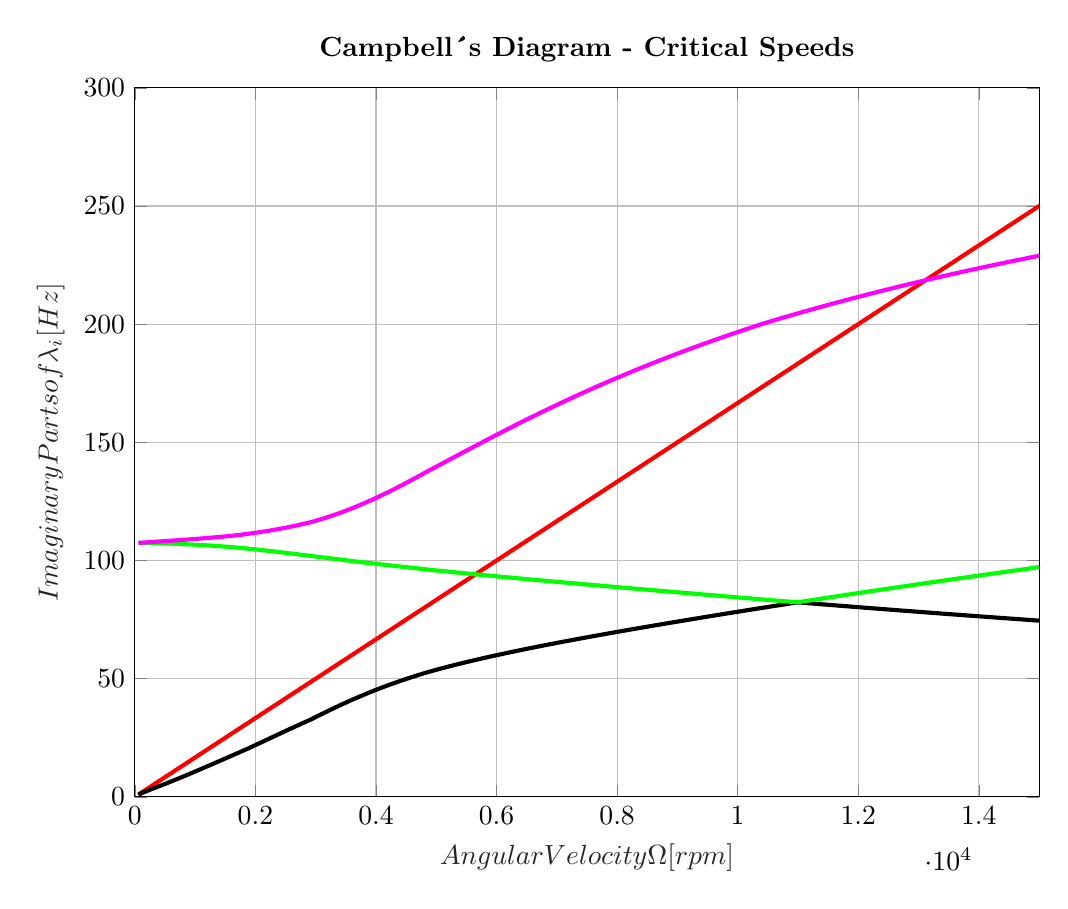
\begin{tikzpicture}

\begin{axis}[%
width=4.521in,
height=3.545in,
at={(0.758in,0.502in)},
scale only axis,
xmin=0,
xmax=15000,
xlabel style={font=\color{white!15!black}},
xlabel={$\text{Angular Velocity }\Omega\text{ [rpm]}$},
ymin=0,
ymax=300,
ylabel style={font=\color{white!15!black}},
ylabel={$\text{Imaginary Parts of }\lambda{}_\text{i}\text{ [Hz]}$},
axis background/.style={fill=white},
title style={font=\bfseries},
title={Campbell´s Diagram - Critical Speeds},
xmajorgrids,
ymajorgrids
]
\addplot [color=red, line width=1.5pt, forget plot]
  table[row sep=crcr]{%
60	1\\
120	2\\
180	3\\
240	4\\
300	5\\
360	6\\
420	7\\
480	8\\
540	9\\
600	10\\
660	11\\
720	12\\
780	13\\
840	14\\
900	15\\
960	16\\
1020	17\\
1080	18\\
1140	19\\
1200	20\\
1260	21\\
1320	22\\
1380	23\\
1440	24\\
1500	25\\
1560	26\\
1620	27\\
1680	28\\
1740	29\\
1800	30\\
1860	31\\
1920	32\\
1980	33\\
2040	34\\
2100	35\\
2160	36\\
2220	37\\
2280	38\\
2340	39\\
2400	40\\
2460	41\\
2520	42\\
2580	43\\
2640	44\\
2700	45\\
2760	46\\
2820	47\\
2880	48\\
2940	49\\
3000	50\\
3060	51\\
3120	52\\
3180	53\\
3240	54\\
3300	55\\
3360	56\\
3420	57\\
3480	58\\
3540	59\\
3600	60\\
3660	61\\
3720	62\\
3780	63\\
3840	64\\
3900	65\\
3960	66\\
4020	67\\
4080	68\\
4140	69\\
4200	70\\
4260	71\\
4320	72\\
4380	73\\
4440	74\\
4500	75\\
4560	76\\
4620	77\\
4680	78\\
4740	79\\
4800	80\\
4860	81\\
4920	82\\
4980	83\\
5040	84\\
5100	85\\
5160	86\\
5220	87\\
5280	88\\
5340	89\\
5400	90\\
5460	91\\
5520	92\\
5580	93\\
5640	94\\
5700	95\\
5760	96\\
5820	97\\
5880	98\\
5940	99\\
6000	100\\
6060	101\\
6120	102\\
6180	103\\
6240	104\\
6300	105\\
6360	106\\
6420	107\\
6480	108\\
6540	109\\
6600	110\\
6660	111\\
6720	112\\
6780	113\\
6840	114\\
6900	115\\
6960	116\\
7020	117\\
7080	118\\
7140	119\\
7200	120\\
7260	121\\
7320	122\\
7380	123\\
7440	124\\
7500	125\\
7560	126\\
7620	127\\
7680	128\\
7740	129\\
7800	130\\
7860	131\\
7920	132\\
7980	133\\
8040	134\\
8100	135\\
8160	136\\
8220	137\\
8280	138\\
8340	139\\
8400	140\\
8460	141\\
8520	142\\
8580	143\\
8640	144\\
8700	145\\
8760	146\\
8820	147\\
8880	148\\
8940	149\\
9000	150\\
9060	151\\
9120	152\\
9180	153\\
9240	154\\
9300	155\\
9360	156\\
9420	157\\
9480	158\\
9540	159\\
9600	160\\
9660	161\\
9720	162\\
9780	163\\
9840	164\\
9900	165\\
9960	166\\
10020	167\\
10080	168\\
10140	169\\
10200	170\\
10260	171\\
10320	172\\
10380	173\\
10440	174\\
10500	175\\
10560	176\\
10620	177\\
10680	178\\
10740	179\\
10800	180\\
10860	181\\
10920	182\\
10980	183\\
11040	184\\
11100	185\\
11160	186\\
11220	187\\
11280	188\\
11340	189\\
11400	190\\
11460	191\\
11520	192\\
11580	193\\
11640	194\\
11700	195\\
11760	196\\
11820	197\\
11880	198\\
11940	199\\
12000	200\\
12060	201\\
12120	202\\
12180	203\\
12240	204\\
12300	205\\
12360	206\\
12420	207\\
12480	208\\
12540	209\\
12600	210\\
12660	211\\
12720	212\\
12780	213\\
12840	214\\
12900	215\\
12960	216\\
13020	217\\
13080	218\\
13140	219\\
13200	220\\
13260	221\\
13320	222\\
13380	223\\
13440	224\\
13500	225\\
13560	226\\
13620	227\\
13680	228\\
13740	229\\
13800	230\\
13860	231\\
13920	232\\
13980	233\\
14040	234\\
14100	235\\
14160	236\\
14220	237\\
14280	238\\
14340	239\\
14400	240\\
14460	241\\
14520	242\\
14580	243\\
14640	244\\
14700	245\\
14760	246\\
14820	247\\
14880	248\\
14940	249\\
15000	250\\
15060	251\\
15120	252\\
15180	253\\
15240	254\\
15300	255\\
15360	256\\
15420	257\\
15480	258\\
15540	259\\
15600	260\\
15660	261\\
15720	262\\
15780	263\\
15840	264\\
15900	265\\
15960	266\\
16020	267\\
16080	268\\
16140	269\\
16200	270\\
16260	271\\
16320	272\\
16380	273\\
16440	274\\
16500	275\\
16560	276\\
16620	277\\
16680	278\\
16740	279\\
16800	280\\
16860	281\\
16920	282\\
16980	283\\
17040	284\\
17100	285\\
17160	286\\
17220	287\\
17280	288\\
17340	289\\
17400	290\\
17460	291\\
17520	292\\
17580	293\\
17640	294\\
17700	295\\
17760	296\\
17820	297\\
17880	298\\
17940	299\\
};
\addplot [color=black, line width=1.5pt, forget plot]
  table[row sep=crcr]{%
60	0.874971235678326\\
120	1.65028234178887\\
180	2.29003417707735\\
240	2.90211216554813\\
300	3.49752599609471\\
360	4.08587592863577\\
420	4.66448336554673\\
480	5.2648752878829\\
540	5.88506694682445\\
600	6.50272881155821\\
660	7.11841170331159\\
720	7.73227894313637\\
780	8.35275038174122\\
840	8.99652621579654\\
900	9.64287859315492\\
960	10.2919983209097\\
1020	10.9439796393002\\
1080	11.5988248344515\\
1140	12.2564478558825\\
1200	12.9166777712831\\
1260	13.5785713117566\\
1320	14.2414574049218\\
1380	14.9055644508479\\
1440	15.5708652281663\\
1500	16.2372873765126\\
1560	16.9047165373701\\
1620	17.5729999442359\\
1680	18.2419496394459\\
1740	18.9113428750971\\
1800	19.5809276781827\\
1860	20.2504220784664\\
1920	20.9459482307154\\
1980	21.6626562412702\\
2040	22.3802835780286\\
2100	23.0984761494743\\
2160	23.8168618984701\\
2220	24.5350529200253\\
2280	25.2526466909656\\
2340	25.9692267415315\\
2400	26.6843658298727\\
2460	27.3976266046195\\
2520	28.1085651007425\\
2580	28.8167310616445\\
2640	29.521670677902\\
2700	30.2229303730059\\
2760	30.9200571060524\\
2820	31.6126030621734\\
2880	32.3001260700648\\
2940	32.9965769598336\\
3000	33.7666328773794\\
3060	34.530473746824\\
3120	35.2874221413458\\
3180	36.0368293490531\\
3240	36.7780815504769\\
3300	37.5106064333073\\
3360	38.2338733010946\\
3420	38.947400723206\\
3480	39.6507585861593\\
3540	40.3435682287762\\
3600	41.0255074070328\\
3660	41.6963110206504\\
3720	42.355764317333\\
3780	43.0037110711102\\
3840	43.6400475958616\\
3900	44.2647174191144\\
3960	44.8777161873039\\
4020	45.4790801523487\\
4080	46.0688886995667\\
4140	46.647256161092\\
4200	47.2143329277274\\
4260	47.7702956409862\\
4320	48.3153492380047\\
4380	48.8497173577916\\
4440	49.3736452092431\\
4500	49.8873892794849\\
4560	50.3912105711955\\
4620	50.8853980740008\\
4680	51.3702314523437\\
4740	51.8459968376434\\
4800	52.3129831074109\\
4860	52.7714775492181\\
4920	53.2114063561139\\
4980	53.6318831903345\\
5040	54.0457155280634\\
5100	54.4531570998982\\
5160	54.8544556946398\\
5220	55.2498477475872\\
5280	55.6395609152914\\
5340	56.0238191054382\\
5400	56.402832488164\\
5460	56.7768070637616\\
5520	57.1459383809535\\
5580	57.5104141975662\\
5640	57.8704157955585\\
5700	58.2261168529434\\
5760	58.5776829122139\\
5820	58.9252748745487\\
5880	59.2690418584976\\
5940	59.6091333258985\\
6000	59.9456866463015\\
6060	60.278836908745\\
6120	60.6087113782215\\
6180	60.9354337694301\\
6240	61.2591207174227\\
6300	61.5798846811075\\
6360	61.8978336037226\\
6420	62.2130709924424\\
6480	62.5256942590559\\
6540	62.835799046335\\
6600	63.1434756911398\\
6660	63.4488117208134\\
6720	63.7518899765025\\
6780	64.0527908812874\\
6840	64.3515900571127\\
6900	64.6483624734165\\
6960	64.9431782178254\\
7020	65.236104672285\\
7080	65.527208303802\\
7140	65.8165492324286\\
7200	66.1041899993393\\
7260	66.3901867978064\\
7320	66.6745961897116\\
7380	66.9574708956231\\
7440	67.2388620574515\\
7500	67.5188210448238\\
7560	67.7973927713324\\
7620	68.0746238668184\\
7680	68.350557819417\\
7740	68.6252379001533\\
7800	68.8987037388456\\
7860	69.1709938007465\\
7920	69.4421461\\
7980	69.712196750918\\
8040	69.9811803183804\\
8100	70.249129593971\\
8160	70.5160757746199\\
8220	70.7820493311958\\
8280	71.0470795401074\\
8340	71.3111935625834\\
8400	71.5744193425002\\
8460	71.8367802986837\\
8520	72.0983000742772\\
8580	72.3590041853098\\
8640	72.6189092985473\\
8700	72.878040174709\\
8760	73.136414344701\\
8820	73.394053249129\\
8880	73.6509657636732\\
8940	73.9071767171253\\
9000	74.1626938137736\\
9060	74.417537960681\\
9120	74.6717161742831\\
9180	74.9252424128807\\
9240	75.1781286317722\\
9300	75.430384522173\\
9360	75.6820198814565\\
9420	75.9330425358877\\
9480	76.1834586326292\\
9540	76.4332764961505\\
9600	76.6825048607542\\
9660	76.9311477289735\\
9720	77.1792088267549\\
9780	77.4266924568041\\
9840	77.6736043356203\\
9900	77.9199486610357\\
9960	78.1657269361672\\
10020	78.4109442633865\\
10080	78.6556016125088\\
10140	78.8997030952633\\
10200	79.143247684255\\
10260	79.3862387959495\\
10320	79.6286774182963\\
10380	79.8705721184434\\
10440	80.1119173903067\\
10500	80.3527760644489\\
10560	80.593205698259\\
10620	80.8331622454144\\
10680	81.0726483980372\\
10740	81.311661649621\\
10800	81.5501980901488\\
10860	81.7882610256689\\
10920	82.0258503013461\\
10980	82.2629611127702\\
11040	82.2246976940528\\
11100	82.1004960975746\\
11160	81.9765436243732\\
11220	81.8528481580071\\
11280	81.729420118185\\
11340	81.606244602735\\
11400	81.4833288527217\\
11460	81.3606777433785\\
11520	81.2382927817483\\
11580	81.1161689104734\\
11640	80.9943132321542\\
11700	80.8727266611065\\
11760	80.7514101634066\\
11820	80.6303644806269\\
11880	80.5095781013566\\
11940	80.3890680215667\\
12000	80.2688170228538\\
12060	80.14883301285\\
12120	80.0291165600196\\
12180	79.9096707148795\\
12240	79.7904843618206\\
12300	79.671558284838\\
12360	79.5528940283344\\
12420	79.434500824243\\
12480	79.3163540873091\\
12540	79.1984701362982\\
12600	79.0808426920816\\
12660	78.9634761464361\\
12720	78.846352992154\\
12780	78.7294843694103\\
12840	78.6128691439155\\
12900	78.4965002973703\\
12960	78.3803721997643\\
13020	78.2645002068745\\
13080	78.1488599263504\\
13140	78.0334757710933\\
13200	77.9183252686202\\
13260	77.8034123429967\\
13320	77.6887310033188\\
13380	77.574290138813\\
13440	77.4600835254443\\
13500	77.3461095564699\\
13560	77.2323655640607\\
13620	77.1188490012141\\
13680	77.0055636158265\\
13740	76.8924990396833\\
13800	76.7796680846399\\
13860	76.6670544331906\\
13920	76.5546663108671\\
13980	76.4424903153601\\
14040	76.3305373708341\\
14100	76.2188070192804\\
14160	76.1072834618601\\
14220	75.99598725353\\
14280	75.884893213376\\
14340	75.7740274610102\\
14400	75.6633617566415\\
14460	75.5529139550454\\
14520	75.4426644565845\\
14580	75.3326330494156\\
14640	75.2228133010081\\
14700	75.113188710028\\
14760	75.0037794725985\\
14820	74.8945749766065\\
14880	74.7855642479056\\
14940	74.6767685957737\\
15000	74.5681653698277\\
15060	74.4597688301189\\
15120	74.3515752395572\\
15180	74.2435811493815\\
15240	74.1357825665933\\
15300	74.0281838955838\\
15360	73.9207803050883\\
15420	73.8135805422962\\
15480	73.7065740360517\\
15540	73.5997658614502\\
15600	73.4931469508739\\
15660	73.3867237033657\\
15720	73.2804913537815\\
15780	73.1744624334474\\
15840	73.0686206866147\\
15900	72.9629718287934\\
15960	72.857513064703\\
16020	72.7522424327762\\
16080	72.6471719911193\\
16140	72.5422900337659\\
16200	72.43759266349\\
16260	72.3330907330171\\
16320	72.228775064032\\
16380	72.1246456303719\\
16440	72.0207100861059\\
16500	71.9169553321222\\
16560	71.8133957082014\\
16620	71.71002347392\\
16680	71.6068301617355\\
16740	71.5038284880118\\
16800	71.4010099054537\\
16860	71.2983796158417\\
16920	71.1959361648195\\
16980	71.0936773797552\\
17040	70.9915996065137\\
17100	70.889708821151\\
17160	70.7880038149882\\
17220	70.6864831932118\\
17280	70.5851449138499\\
17340	70.4839878334988\\
17400	70.38301475327\\
17460	70.2822263862518\\
17520	70.1816192206949\\
17580	70.081194662031\\
17640	69.9809567712123\\
17700	69.8808938253025\\
17760	69.7810117567439\\
17820	69.6813208937371\\
17880	69.581805426246\\
17940	69.4824660045069\\
};
\addplot [color=green, line width=1.5pt, forget plot]
  table[row sep=crcr]{%
60	107.406805161813\\
120	107.397589804316\\
180	107.38327630972\\
240	107.363987582276\\
300	107.340650404373\\
360	107.312989988406\\
420	107.281284706434\\
480	107.244138171917\\
540	107.201285512702\\
600	107.1539039473\\
660	107.102161793738\\
720	107.046239738925\\
780	106.985847771243\\
840	106.919865486159\\
900	106.849315462609\\
960	106.774244646795\\
1020	106.69468355488\\
1080	106.610676059192\\
1140	106.522265469744\\
1200	106.4294945806\\
1260	106.330622069012\\
1320	106.225981033169\\
1380	106.116541401448\\
1440	106.002337307745\\
1500	105.883431793869\\
1560	105.759902100817\\
1620	105.631837262856\\
1680	105.499356381336\\
1740	105.362573143114\\
1800	105.221636106733\\
1860	105.076700904002\\
1920	104.924894092617\\
1980	104.766753263646\\
2040	104.604753001115\\
2100	104.439123672906\\
2160	104.270110550111\\
2220	104.097975507432\\
2280	103.922976586632\\
2340	103.745374953051\\
2400	103.565436865955\\
2460	103.383421141548\\
2520	103.199590954223\\
2580	103.014197216567\\
2640	102.827473563143\\
2700	102.639661411305\\
2760	102.450972945906\\
2820	102.261621280615\\
2880	102.071790900172\\
2940	101.881749481352\\
3000	101.692069640573\\
3060	101.50253945543\\
3120	101.313283815452\\
3180	101.124408957826\\
3240	100.936020783143\\
3300	100.748211630114\\
3360	100.561056427997\\
3420	100.374623311088\\
3480	100.188983645416\\
3540	100.004171142395\\
3600	99.8202425074528\\
3660	99.6372377453624\\
3720	99.4551799395959\\
3780	99.2741021247057\\
3840	99.0940199667411\\
3900	98.9149514930112\\
3960	98.7369091132477\\
4020	98.5599035279277\\
4080	98.3839365699301\\
4140	98.2090145888631\\
4200	98.0351341760411\\
4260	97.8622956976233\\
4320	97.6904909955505\\
4380	97.5197131675484\\
4440	97.3499519929102\\
4500	97.1812132592794\\
4560	97.0134735545946\\
4620	96.8467241324884\\
4680	96.6809442374607\\
4740	96.5161390449857\\
4800	96.352281498789\\
4860	96.1893647259657\\
4920	96.0294652193923\\
4980	95.872953149955\\
5040	95.7173370505758\\
5100	95.5625960219751\\
5160	95.4087041811349\\
5220	95.2556404469075\\
5280	95.1033821435004\\
5340	94.9519123078428\\
5400	94.8012049076441\\
5460	94.6512369609839\\
5520	94.50199117552\\
5580	94.3534506271905\\
5640	94.2055896804913\\
5700	94.0583936166039\\
5760	93.9118432230243\\
5820	93.7659163830878\\
5880	93.62060113165\\
5940	93.4758757584545\\
6000	93.331729301577\\
6060	93.1881389135417\\
6120	93.0450872098825\\
6180	92.9025635039387\\
6240	92.7605455723391\\
6300	92.6190288725217\\
6360	92.4779904201492\\
6420	92.3374151531754\\
6480	92.1972926742415\\
6540	92.0576086283796\\
6600	91.9183466010284\\
6660	91.7794942459478\\
6720	91.6410378427241\\
6780	91.5029634350833\\
6840	91.3652649044511\\
6900	91.2279193254945\\
6960	91.0909266262641\\
7020	90.9542628993366\\
7080	90.8179239636487\\
7140	90.6818996741034\\
7200	90.5461727025086\\
7260	90.4107382927456\\
7320	90.2755778065945\\
7380	90.1406882942629\\
7440	90.0060580484404\\
7500	89.871671639673\\
7560	89.7375263496846\\
7620	89.6036091845198\\
7680	89.4699112243511\\
7740	89.3364241197363\\
7800	89.2031380249837\\
7860	89.0700490129288\\
7920	88.9371446128117\\
7980	88.8044167877677\\
8040	88.6718626532602\\
8100	88.5394713478994\\
8160	88.4072361629258\\
8220	88.2751515949533\\
8280	88.1432132758276\\
8340	88.0114224392963\\
8400	87.8797510096138\\
8460	87.7482206317219\\
8520	87.6168184501182\\
8580	87.4855394475982\\
8640	87.3543785374832\\
8700	87.2233328094276\\
8760	87.0924134820546\\
8820	86.9615885857729\\
8880	86.8308948660143\\
8940	86.7003084243912\\
9000	86.5698344765754\\
9060	86.4394658817929\\
9120	86.3092269023702\\
9180	86.1790932565008\\
9240	86.0490847893578\\
9300	85.9191880369986\\
9360	85.7894209899142\\
9420	85.6597686968738\\
9480	85.5302612243312\\
9540	85.4008866664162\\
9600	85.2716451396519\\
9660	85.1425448638193\\
9720	85.0135890144358\\
9780	84.8847979805932\\
9840	84.7561662534641\\
9900	84.6276915946072\\
9960	84.499387881047\\
10020	84.3712547907969\\
10080	84.2433099870805\\
10140	84.1155458020941\\
10200	83.9879775505884\\
10260	83.860613436112\\
10320	83.7334506751925\\
10380	83.6064892945436\\
10440	83.4797438673752\\
10500	83.353227416285\\
10560	83.2269391087109\\
10620	83.1008649913361\\
10680	82.9749997326409\\
10740	82.8493664738399\\
10800	82.7239570981312\\
10860	82.5987788159368\\
10920	82.4738369121576\\
10980	82.3491431721571\\
11040	82.4995975114542\\
11100	82.7357599793743\\
11160	82.9714487359736\\
11220	83.2066646981587\\
11280	83.4414040717418\\
11340	83.6756743625754\\
11400	83.9094780754288\\
11460	84.1428115899759\\
11520	84.3756814202394\\
11580	84.6080899433121\\
11640	84.8400351372031\\
11700	85.0715199736719\\
11760	85.3025481849178\\
11820	85.5331253601183\\
11880	85.7632541727655\\
11940	85.9929342818708\\
12000	86.2221688541459\\
12060	86.4509668064684\\
12120	86.6793257182842\\
12180	86.9072503596821\\
12240	87.1347463949298\\
12300	87.361818855648\\
12360	87.5884671603202\\
12420	87.814693241934\\
12480	88.0405071429826\\
12540	88.2659089210155\\
12600	88.4909059826409\\
12660	88.7154934315393\\
12720	88.9396886115041\\
12780	89.1634846593095\\
12840	89.3868883752269\\
12900	89.6099020806981\\
12960	89.8325342562156\\
13020	90.0547809493271\\
13080	90.2766551405118\\
13140	90.498151464183\\
13200	90.7192823262608\\
13260	90.9400407274587\\
13320	91.1604404173782\\
13380	91.3804796072083\\
13440	91.6001613094644\\
13500	91.8194949766663\\
13560	92.0384726809826\\
13620	92.2571095218017\\
13680	92.475400897673\\
13740	92.693350179102\\
13800	92.9109668278794\\
13860	93.1282463129411\\
13920	93.3451966262433\\
13980	93.5618190044285\\
14040	93.7781185621439\\
14100	93.9940906937967\\
14160	94.2097497694778\\
14220	94.4250855825205\\
14280	94.6401121111834\\
14340	94.8548215793602\\
14400	95.0692276356609\\
14460	95.2833245940848\\
14520	95.4971200124144\\
14580	95.7106110047248\\
14640	95.9238007693269\\
14700	96.136696918209\\
14760	96.3492955807543\\
14820	96.5616023844129\\
14880	96.7736207350613\\
14940	96.9853447365024\\
15000	97.1967910011334\\
15060	97.4079445399229\\
15120	97.6188154847172\\
15180	97.8294059069494\\
15240	98.0397235168008\\
15300	98.2497573755157\\
15360	98.459521738866\\
15420	98.6690035826204\\
15480	98.8782198553571\\
15540	99.0871620850204\\
15600	99.2958388021641\\
15660	99.5042482422782\\
15720	99.7123949437628\\
15780	99.9202729705853\\
15840	100.127889347403\\
15900	100.335243087931\\
15960	100.542338737003\\
16020	100.749177073527\\
16080	100.955757452795\\
16140	101.162083596599\\
16200	101.368151417156\\
16260	101.573971695741\\
16320	101.77953644811\\
16380	101.984851088003\\
16440	102.189918337662\\
16500	102.394739028217\\
16560	102.599310555856\\
16620	102.803634868969\\
16680	103.007715916049\\
16740	103.211553705675\\
16800	103.415146884398\\
16860	103.618503979853\\
16920	103.82161399704\\
16980	104.024489623313\\
17040	104.227125409269\\
17100	104.429520279727\\
17160	104.631683893889\\
17220	104.833606964615\\
17280	105.03530138376\\
17340	105.23675833222\\
17400	105.437985377882\\
17460	105.638972188997\\
17520	105.839734685599\\
17580	106.040265558746\\
17640	106.240567947614\\
17700	106.440648727792\\
17760	106.640491923577\\
17820	106.840106504677\\
17880	107.039496287743\\
17940	107.238667656429\\
};
\addplot [color=mycolor1, line width=1.5pt, forget plot]
  table[row sep=crcr]{%
60	107.473294103906\\
120	107.574980911479\\
180	107.677494965992\\
240	107.780822471265\\
300	107.88189904721\\
360	107.983266415924\\
420	108.084272581532\\
480	108.190576033492\\
540	108.297392183312\\
600	108.403283265453\\
660	108.509410769961\\
720	108.617157293604\\
780	108.726510803889\\
840	108.833943775075\\
900	108.943190499153\\
960	109.055069210575\\
1020	109.170414109815\\
1080	109.29007463738\\
1140	109.414897092724\\
1200	109.545776949552\\
1260	109.671753337529\\
1320	109.796921759449\\
1380	109.928238238032\\
1440	110.066171668789\\
1500	110.211186834715\\
1560	110.363680461532\\
1620	110.524047261735\\
1680	110.692683070704\\
1740	110.869888255038\\
1800	111.056031824317\\
1860	111.251407338124\\
1920	111.454516284575\\
1980	111.66538224855\\
2040	111.885373768123\\
2100	112.114673845776\\
2160	112.353420967238\\
2220	112.601752816223\\
2280	112.859830956495\\
2340	113.127763211389\\
2400	113.405679403629\\
2460	113.693706307707\\
2520	113.991975494327\\
2580	114.300599936008\\
2640	114.61972464021\\
2700	114.949459758467\\
2760	115.289926735415\\
2820	115.641276501182\\
2880	116.003609929025\\
2940	116.3844864339\\
3000	116.820014881272\\
3060	117.271176227857\\
3120	117.738269475841\\
3180	118.221536968492\\
3240	118.72122531913\\
3300	119.237493183481\\
3360	119.770465271588\\
3420	120.320212078629\\
3480	120.886760566123\\
3540	121.470042904367\\
3600	122.069989218894\\
3660	122.686394381153\\
3720	123.319073109879\\
3780	123.967736420068\\
3840	124.632019469772\\
3900	125.311573116527\\
3960	126.00592297718\\
4020	126.714613281026\\
4080	127.437086131707\\
4140	128.17283595322\\
4200	128.921214923063\\
4260	129.681661008085\\
4320	130.453492604371\\
4380	131.236080208799\\
4440	132.028765750609\\
4500	132.830853802631\\
4560	133.641727227253\\
4620	134.460655322766\\
4680	135.286978992206\\
4740	136.120062076654\\
4800	136.959243008898\\
4860	137.803910126356\\
4920	138.633927631452\\
4980	139.443536266893\\
5040	140.254780252349\\
5100	141.067269030276\\
5160	141.880552187356\\
5220	142.694265861102\\
5280	143.508109163431\\
5340	144.3216718601\\
5400	145.134653691336\\
5460	145.946724397451\\
5520	146.757599400658\\
5580	147.567038846842\\
5640	148.374771076926\\
5700	149.180531696946\\
5760	149.984112937539\\
5820	150.785274785508\\
5880	151.58389342693\\
5940	152.379682167082\\
6000	153.172549677341\\
6060	153.962304331699\\
6120	154.748790953851\\
6180	155.531882712002\\
6240	156.311436501955\\
6300	157.08737174656\\
6360	157.859553171744\\
6420	158.627883850797\\
6480	159.392288752298\\
6540	160.152691595636\\
6600	160.908989870718\\
6660	161.661135835026\\
6720	162.409073298255\\
6780	163.152719218086\\
6840	163.892098496255\\
6900	164.627069400533\\
6960	165.357666899146\\
7020	166.083841064999\\
7080	166.805532633549\\
7140	167.522793680922\\
7200	168.235534606193\\
7260	168.943804359005\\
7320	169.647532838435\\
7380	170.346737385524\\
7440	171.041443456526\\
7500	171.731557876299\\
7560	172.417175893935\\
7620	173.098270196268\\
7680	173.774860273428\\
7740	174.446911424496\\
7800	175.114464123412\\
7860	175.777555203701\\
7920	176.4361635607\\
7980	177.090320953165\\
8040	177.740020509849\\
8100	178.385293902799\\
8160	179.026176390868\\
8220	179.662678515987\\
8280	180.294817019304\\
8340	180.922635114408\\
8400	181.546062069348\\
8460	182.16528237205\\
8520	182.780236215082\\
8580	183.390904523004\\
8640	183.997371256433\\
8700	184.599683233635\\
8760	185.19786299681\\
8820	185.791763817937\\
8880	186.38172611371\\
8940	186.967522238666\\
9000	187.549314838202\\
9060	188.127038962957\\
9120	188.700838791251\\
9180	189.270615016038\\
9240	189.836544106708\\
9300	190.398511382292\\
9360	190.956596589519\\
9420	191.510817242782\\
9480	192.061312175872\\
9540	192.608011627812\\
9600	193.150918046199\\
9660	193.690054029698\\
9720	194.225545848501\\
9780	194.757424035883\\
9840	195.285654565507\\
9900	195.810265671666\\
9960	196.331280219399\\
10020	196.848721676973\\
10080	197.362685954744\\
10140	197.87307807145\\
10200	198.380112117835\\
10260	198.883705164886\\
10320	199.383926025762\\
10380	199.880666952704\\
10440	200.374050570655\\
10500	200.849880602571\\
10560	201.308192236029\\
10620	201.763911939734\\
10680	202.216931318281\\
10740	202.667368747792\\
10800	203.115261657687\\
10860	203.560562562571\\
10920	204.003265659598\\
10980	204.443517340955\\
11040	204.881301347771\\
11100	205.316534486292\\
11160	205.749250172523\\
11220	206.179516208456\\
11280	206.607452013988\\
11340	207.032886800928\\
11400	207.455873871063\\
11460	207.876498933328\\
11520	208.294715817003\\
11580	208.710484451327\\
11640	209.123982082306\\
11700	209.535138715455\\
11760	209.944000590572\\
11820	210.350545959037\\
11880	210.75474863429\\
11940	211.156724945335\\
12000	211.55637879921\\
12060	211.953792076771\\
12120	212.348985392656\\
12180	212.742015474269\\
12240	213.132793851173\\
12300	213.52131465042\\
12360	213.907692520385\\
12420	214.292023361138\\
12480	214.674056006987\\
12540	215.054061292272\\
12600	215.431874639359\\
12660	215.807706940317\\
12720	216.181285982226\\
12780	216.552847284437\\
12840	216.922379266738\\
12900	217.289857457898\\
12960	217.655207133186\\
13020	218.018668158465\\
13080	218.379998694936\\
13140	218.739464824059\\
13200	219.096874382526\\
13260	219.452339808987\\
13320	219.805805560564\\
13380	220.157323328978\\
13440	220.506980283672\\
13500	220.854670326977\\
13560	221.200510749375\\
13620	221.544415734049\\
13680	221.886467163901\\
13740	222.226646699945\\
13800	222.565006606376\\
13860	222.901553467629\\
13920	223.236229791854\\
13980	223.56907807637\\
14040	223.900105981106\\
14100	224.229442555465\\
14160	224.55688781852\\
14220	224.882678421051\\
14280	225.206633610789\\
14340	225.52896499979\\
14400	225.849477162884\\
14460	226.168316062651\\
14520	226.485357818184\\
14580	226.800819156005\\
14640	227.114646521585\\
14700	227.426681950969\\
14760	227.737135725918\\
14820	228.045965897999\\
14880	228.353087223076\\
14940	228.658678078837\\
15000	228.962535944072\\
15060	229.264910272022\\
15120	229.565706349428\\
15180	229.864923875705\\
15240	230.162512469022\\
15300	230.458629941365\\
15360	230.753120644747\\
15420	231.046193195456\\
15480	231.337680167242\\
15540	231.627725590281\\
15600	231.916194149643\\
15660	232.203185805865\\
15720	232.488654311966\\
15780	232.77279283461\\
15840	233.055434197934\\
15900	233.33658873553\\
15960	233.616350573647\\
16020	233.894623039736\\
16080	234.171574010409\\
16140	234.447132984997\\
16200	234.721242663667\\
16260	234.993997560017\\
16320	235.265377919508\\
16380	235.535380670954\\
16440	235.804065625868\\
16500	236.071371146208\\
16560	236.337414554582\\
16620	236.602114815809\\
16680	236.865439730607\\
16740	237.127519800893\\
16800	237.388274712091\\
16860	237.647773647253\\
16920	237.906012212928\\
16980	238.16298004698\\
17040	238.418649990758\\
17100	238.673118763934\\
17160	238.926369031509\\
17220	239.178415680613\\
17280	239.429164495322\\
17340	239.678726970931\\
17400	239.927067820581\\
17460	240.174275751367\\
17520	240.420272218437\\
17580	240.665115430512\\
17640	240.908804283742\\
17700	241.151268919907\\
17760	241.392591057997\\
17820	241.632894014791\\
17880	241.872006737969\\
17940	242.109907045657\\
};
\end{axis}
\end{tikzpicture}%
    \caption{Campbell diagram of Hydrodynamic Bearing}
    \label{fig:hydrodynamic_bearing_campbell}
\end{figure}


\subsubsection{Operational range}
The operation range can be determined from figure \ref{fig:hydrodynamic_bearing_campbell} to be approximatly 7500 rpm.

\subsection{Rotor Bearing Stability Limit}
Instability occurs when the real part of the eigenvalues are positive.

\subsubsection{Maximum angular velocity}
To check for instability, the real parts of the eigenvalues are compared to the angular velocity in figure \ref{fig:hydrodynamic_bearing_eigenvalues}.
\begin{figure}[ht]
    \centering
    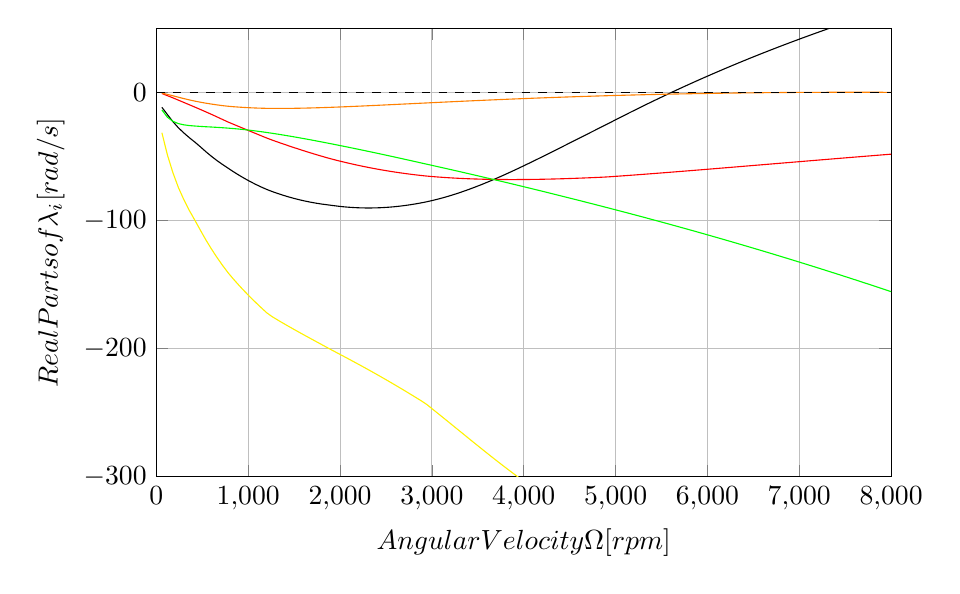
\begin{tikzpicture}

\begin{axis}[%
width=0.9\linewidth,
height=0.6\linewidth,
ymin=-300,
ymax=50,
xmin=0,
xmax=8000,
xlabel={$\text{Angular Velocity }\Omega\text{ [rpm]}$},
ylabel={$\text{Real Parts of }\lambda{}_\text{i}\text{ [rad/s]}$},
grid=major,
]
\addplot [color=black, forget plot]
  table[row sep=crcr]{%
60	-11.7378188663084\\
120	-17.4305641796133\\
180	-22.9287996607167\\
240	-27.7571053061481\\
300	-31.8168875588271\\
360	-35.5510837506116\\
420	-38.9577340966405\\
480	-42.6441859040235\\
540	-46.4707787514977\\
600	-50.0346572560797\\
660	-53.3380728475882\\
720	-56.3800215902463\\
780	-59.2331835623643\\
840	-62.0823494250039\\
900	-64.7671944451812\\
960	-67.2911713097243\\
1020	-69.6566956631429\\
1080	-71.8653395855256\\
1140	-73.9179834930207\\
1200	-75.8149444570892\\
1260	-77.4874357911471\\
1320	-79.0009969575832\\
1380	-80.4050893182093\\
1440	-81.7012887466219\\
1500	-82.8908994082669\\
1560	-83.9750054940951\\
1620	-84.9545149231793\\
1680	-85.8301997303113\\
1740	-86.6027339742371\\
1800	-87.2727181481711\\
1860	-87.8407144866309\\
1920	-88.4083161633821\\
1980	-88.9588891163609\\
2040	-89.4166529257057\\
2100	-89.781956202306\\
2160	-90.0551833025719\\
2220	-90.2367674106098\\
2280	-90.3272036723401\\
2340	-90.3270686289457\\
2400	-90.2370309153059\\
2460	-90.0578653421107\\
2520	-89.7904600289643\\
2580	-89.4358336373275\\
2640	-88.9951338877343\\
2700	-88.4696569597766\\
2760	-87.8608449134132\\
2820	-87.1702852672848\\
2880	-86.3997300651424\\
2940	-85.547071153193\\
3000	-84.5844070535899\\
3060	-83.5275138588301\\
3120	-82.3791265291541\\
3180	-81.1422797779227\\
3240	-79.8202719977605\\
3300	-78.4166752934921\\
3360	-76.9352827848105\\
3420	-75.3800913466495\\
3480	-73.7552568651064\\
3540	-72.0650858616293\\
3600	-70.3139564867685\\
3660	-68.5063252116507\\
3720	-66.6466583974228\\
3780	-64.7394112488614\\
3840	-62.7890030542976\\
3900	-60.7997561805557\\
3960	-58.7759055211068\\
4020	-56.7215431783251\\
4080	-54.6406225387765\\
4140	-52.5369119231958\\
4200	-50.4140228914593\\
4260	-48.2753518056414\\
4320	-46.1241191424078\\
4380	-43.9633332526793\\
4440	-41.7958036615159\\
4500	-39.62411330846\\
4560	-37.4507164509088\\
4620	-35.2778053238786\\
4680	-33.1074264845061\\
4740	-30.9414280361321\\
4800	-28.7815060929244\\
4860	-26.6291875864728\\
4920	-24.4462819284045\\
4980	-22.2312053296088\\
5040	-20.033192502541\\
5100	-17.8527750678401\\
5160	-15.690413423151\\
5220	-13.5464893321386\\
5280	-11.4213171246916\\
5340	-9.31514664724817\\
5400	-7.22818597639497\\
5460	-5.16058440122031\\
5520	-3.11244563193185\\
5580	-1.08383168835578\\
5640	0.925226328195507\\
5700	2.9147310798752\\
5760	4.88471670035542\\
5820	6.83524426571491\\
5880	8.76638937350834\\
5940	10.678258615205\\
6000	12.5709701395126\\
6060	14.4446595525311\\
6120	16.2994682043848\\
6180	18.1355686869869\\
6240	19.953120153122\\
6300	21.7523163993411\\
6360	23.5333357482089\\
6420	25.2963767770428\\
6480	27.0416343054815\\
6540	28.7693214468546\\
6600	30.4796321825131\\
6660	32.1727963941115\\
6720	33.8490174384334\\
6780	35.5085106043674\\
6840	37.1515028261204\\
6900	38.7781960741334\\
6960	40.3888295060532\\
7020	41.9836066175374\\
7080	43.5627565171574\\
7140	45.1264898897773\\
7200	46.6750339664741\\
7260	48.2086052895946\\
7320	49.7274147676031\\
7380	51.2316825406613\\
7440	52.7216281939333\\
7500	54.1974649243231\\
7560	55.6594002146994\\
7620	57.1076509871004\\
7680	58.5424278713219\\
7740	59.963945540737\\
7800	61.3724023128967\\
7860	62.768013333124\\
7920	64.150976476688\\
7980	65.5215064449926\\
8040	66.8798043507317\\
8100	68.226069758724\\
8160	69.5604942839992\\
8220	70.8832889312726\\
8280	72.1946439309145\\
8340	73.4947663742575\\
8400	74.7838258395087\\
8460	76.0620276726354\\
8520	77.3296027149088\\
8580	78.5866978098187\\
8640	79.8334244915922\\
8700	81.0701160613009\\
8760	82.2968463659545\\
8820	83.5138603641425\\
8880	84.7213004956291\\
8940	85.9193440166648\\
9000	87.108097330628\\
9060	88.2878701516301\\
9120	89.458757704331\\
9180	90.6208299487751\\
9240	91.7743829672856\\
9300	92.9195296198763\\
9360	94.0563548475906\\
9420	95.1850971187452\\
9480	96.3058410039506\\
9540	97.4187028838986\\
9600	98.5238904784986\\
9660	99.6214887602578\\
9720	100.711603569552\\
9780	101.794372441988\\
9840	102.869939462614\\
9900	103.938389229929\\
9960	104.999791639116\\
10020	106.054297980151\\
10080	107.102002091418\\
10140	108.142942455749\\
10200	109.17728635128\\
10260	110.205064804802\\
10320	111.226364260951\\
10380	112.241247989815\\
10440	113.24988700145\\
10500	114.244081672753\\
10560	115.223987156484\\
10620	116.198058183678\\
10680	117.166280442917\\
10740	118.128825201081\\
10800	119.085648725391\\
10860	120.036811946146\\
10920	120.982371099348\\
10980	121.922458024833\\
11040	-33.5413557041303\\
11100	-33.3022036791618\\
11160	-33.0656237776559\\
11220	-32.8315363377484\\
11280	-32.6000082678254\\
11340	-32.3709354167391\\
11400	-32.1441487597894\\
11460	-31.9197805360053\\
11520	-31.6976699468114\\
11580	-31.4778305913639\\
11640	-31.2602295373125\\
11700	-31.044815847717\\
11760	-30.8315811181487\\
11820	-30.6204219253917\\
11880	-30.4112355282241\\
11940	-30.2041039080485\\
12000	-29.9990202114919\\
12060	-29.7957952957378\\
12120	-29.5945044138539\\
12180	-29.3950748234683\\
12240	-29.1974954917213\\
12300	-29.0016607993933\\
12360	-28.8076185653309\\
12420	-28.6153385922447\\
12480	-28.4247594705604\\
12540	-28.2358105930605\\
12600	-28.048500252392\\
12660	-27.8628606283154\\
12720	-27.678770682282\\
12780	-27.4962407627785\\
12840	-27.3152143334102\\
12900	-27.1357547612498\\
12960	-26.9577515621525\\
13020	-26.7812493347345\\
13080	-26.6061465044082\\
13140	-26.4324925038637\\
13200	-26.2601612679965\\
13260	-26.0893391925551\\
13320	-25.9197969481705\\
13380	-25.7516219814276\\
13440	-25.5847622363848\\
13500	-25.4191554801889\\
13560	-25.2549304095\\
13620	-25.0918783169595\\
13680	-24.930140219976\\
13740	-24.7696627457025\\
13800	-24.6103612217229\\
13860	-24.4522974120403\\
13920	-24.2954381455943\\
13980	-24.1397419042043\\
14040	-23.9852169838302\\
14100	-23.8318720280828\\
14160	-23.6796265954513\\
14220	-23.5285719501656\\
14280	-23.3785929645904\\
14340	-23.2297698582696\\
14400	-23.0819963590732\\
14460	-22.9353424397587\\
14520	-22.7897425621863\\
14580	-22.645215869294\\
14640	-22.5017637943477\\
14700	-22.3593272265888\\
14760	-22.2179439658214\\
14820	-22.0776009268219\\
14880	-21.9382388763633\\
14940	-21.7999426529566\\
15000	-21.6625815649381\\
15060	-21.5262618672889\\
15120	-21.3909246803089\\
15180	-21.2565582445174\\
15240	-21.1231120575135\\
15300	-20.990656360818\\
15360	-20.8591453397294\\
15420	-20.7286178907851\\
15480	-20.5989830094655\\
15540	-20.4702973722705\\
15600	-20.3425164372076\\
15660	-20.2156528664369\\
15720	-20.0896767949331\\
15780	-19.9646086323446\\
15840	-19.8404289070802\\
15900	-19.7171653112821\\
15960	-19.5947546137236\\
16020	-19.4732128609152\\
16080	-19.3525431473482\\
16140	-19.2327008873555\\
16200	-19.1137669338908\\
16260	-18.9956153299857\\
16320	-18.8783404576789\\
16380	-18.7618969710218\\
16440	-18.6462639159008\\
16500	-18.5314287804087\\
16560	-18.4174167992562\\
16620	-18.3042365103396\\
16680	-18.1918506091494\\
16740	-18.0802468738287\\
16800	-17.9694559936616\\
16860	-17.8593931826759\\
16920	-17.7501646644908\\
16980	-17.641668314105\\
17040	-17.5339513250947\\
17100	-17.4270139982349\\
17160	-17.3207967282763\\
17220	-17.2153432307822\\
17280	-17.1106301947651\\
17340	-17.0066592886886\\
17400	-16.903413582571\\
17460	-16.8009292798025\\
17520	-16.6991269349713\\
17580	-16.5980506769961\\
17640	-16.4976840185084\\
17700	-16.3979868983803\\
17760	-16.2990452056861\\
17820	-16.2007940904637\\
17880	-16.1032273487194\\
17940	-16.0063171038567\\
};
\addplot [color=red, forget plot]
  table[row sep=crcr]{%
60	-0.969384937903058\\
120	-2.65521516397317\\
180	-4.36123924225487\\
240	-6.17418027155545\\
300	-7.97909572491899\\
360	-9.79085548968578\\
420	-11.6174519504166\\
480	-13.4659566583383\\
540	-15.3417066678391\\
600	-17.2623903426656\\
660	-19.2286412035638\\
720	-21.2410475480852\\
780	-23.2225477054987\\
840	-25.0167140561377\\
900	-26.8085207678952\\
960	-28.597029839679\\
1020	-30.381249409488\\
1080	-32.1601038869775\\
1140	-33.9324422201191\\
1200	-35.6970598741125\\
1260	-37.3187272600841\\
1320	-38.8395716325985\\
1380	-40.3329197793937\\
1440	-41.7978390763073\\
1500	-43.2333499211443\\
1560	-44.6384348935439\\
1620	-46.0120870357315\\
1680	-47.3532902644559\\
1740	-48.6610548557197\\
1800	-49.9344426971906\\
1860	-51.172553795662\\
1920	-52.3347252279161\\
1980	-53.4272561876297\\
2040	-54.4796072105369\\
2100	-55.4913127747738\\
2160	-56.4619906085781\\
2220	-57.3913751940509\\
2280	-58.2793881308392\\
2340	-59.1260344912781\\
2400	-59.9314691633287\\
2460	-60.6959832458495\\
2520	-61.4199844959879\\
2580	-62.103979201789\\
2640	-62.7486430942031\\
2700	-63.3546591069296\\
2760	-63.9228510436713\\
2820	-64.4541217556491\\
2880	-64.9494206791367\\
2940	-65.4024233853299\\
3000	-65.7812715687675\\
3060	-66.1272718543412\\
3120	-66.4416086427963\\
3180	-66.7254370357654\\
3240	-66.9799208831966\\
3300	-67.2061988926439\\
3360	-67.4053928961845\\
3420	-67.5786067612941\\
3480	-67.7269027648227\\
3540	-67.8513398651225\\
3600	-67.9529565193245\\
3660	-68.0326924204015\\
3720	-68.0915517201566\\
3780	-68.1304429783306\\
3840	-68.1502460560139\\
3900	-68.1518515117839\\
3960	-68.1360617367548\\
4020	-68.1036861012084\\
4080	-68.0554705322659\\
4140	-67.9921975031075\\
4200	-67.914516661687\\
4260	-67.8231641826347\\
4320	-67.7187514586938\\
4380	-67.6019160826631\\
4440	-67.473308939062\\
4500	-67.3334143686376\\
4560	-67.1827707058669\\
4620	-67.0219811073424\\
4680	-66.851533635879\\
4740	-66.6718699954785\\
4800	-66.4834871674447\\
4860	-66.286824820265\\
4920	-66.0423140983372\\
4980	-65.7443865463432\\
5040	-65.4412147451267\\
5100	-65.1331817571383\\
5160	-64.8205657347035\\
5220	-64.5036814868667\\
5280	-64.1828910071432\\
5340	-63.8583994905338\\
5400	-63.5304981502382\\
5460	-63.1994207843609\\
5520	-62.8653972554058\\
5580	-62.5286839401888\\
5640	-62.1894987553814\\
5700	-61.8480073882011\\
5760	-61.5044126600798\\
5820	-61.1589026612677\\
5880	-60.8116856374558\\
5940	-60.4628417253977\\
6000	-60.1125924764006\\
6060	-59.7610754950891\\
6120	-59.4084135573146\\
6180	-59.0547539206063\\
6240	-58.7002097527238\\
6300	-58.3449166024387\\
6360	-57.9889845809033\\
6420	-57.6325278919875\\
6480	-57.2756360234227\\
6540	-56.9184328698133\\
6600	-56.5609736805871\\
6660	-56.2033966656126\\
6720	-55.8457683119643\\
6780	-55.4881564566834\\
6840	-55.1306874838873\\
6900	-54.7733698221931\\
6960	-54.4163214254124\\
7020	-54.0596244576432\\
7080	-53.7032962379447\\
7140	-53.3474540523165\\
7200	-52.9921436347\\
7260	-52.6374497635434\\
7320	-52.2834125355096\\
7380	-51.930076548586\\
7440	-51.5775449710855\\
7500	-51.2258188905519\\
7560	-50.8749911197653\\
7620	-50.525120694723\\
7680	-50.1762728928957\\
7740	-49.8284611829114\\
7800	-49.4817661235302\\
7860	-49.1362474926033\\
7920	-48.7919425419065\\
7980	-48.4489329400532\\
8040	-48.1072304032866\\
8100	-47.7669168739697\\
8160	-47.4280463838595\\
8220	-47.09067548822\\
8280	-46.754840566873\\
8340	-46.4205858686898\\
8400	-46.0879874645797\\
8460	-45.7571047948542\\
8520	-45.4280116110287\\
8580	-45.1006880094274\\
8640	-44.7751418980879\\
8700	-44.451645582614\\
8760	-44.1300252750912\\
8820	-43.8104589141553\\
8880	-43.4929597334395\\
8940	-43.1775371900718\\
9000	-42.8642181640253\\
9060	-42.5532137849266\\
9120	-42.2444101414406\\
9180	-41.9378037443957\\
9240	-41.6336151380584\\
9300	-41.3318098127595\\
9360	-41.0322840878634\\
9420	-40.7353060292534\\
9480	-40.4407390649151\\
9540	-40.1486153146504\\
9600	-39.8590586583031\\
9660	-39.5720067363264\\
9720	-39.2875395389568\\
9780	-39.0056006541927\\
9840	-38.7262562331818\\
9900	-38.4495411031518\\
9960	-38.1753481559981\\
10020	-37.9037854557107\\
10080	-37.6348156407161\\
10140	-37.3683738776935\\
10200	-37.1046164067432\\
10260	-36.8433714223394\\
10320	-36.5847194581278\\
10380	-36.32858264491\\
10440	-36.07504001615\\
10500	-35.8161419055208\\
10560	-35.5520544995624\\
10620	-35.2909175287444\\
10680	-35.0325910490616\\
10740	-34.7771400317987\\
10800	-34.5245226522789\\
10860	-34.2746610865482\\
10920	-34.0274956603266\\
10980	-33.7831352916686\\
11040	122.856945981418\\
11100	123.785969811777\\
11160	124.709549558721\\
11220	125.627688532953\\
11280	126.54050890873\\
11340	127.447988597491\\
11400	128.35006214198\\
11460	129.246888237721\\
11520	130.138430745028\\
11580	131.024762406955\\
11640	131.905861799105\\
11700	132.781803691095\\
11760	133.652628789689\\
11820	134.518330665475\\
11880	135.378835374882\\
11940	136.234327066566\\
12000	137.084816390653\\
12060	137.930197382836\\
12120	138.770616557186\\
12180	139.606068938465\\
12240	140.436585427733\\
12300	141.262159040568\\
12360	142.082841021355\\
12420	142.898699074447\\
12480	143.709720451007\\
12540	144.51585286331\\
12600	145.317252147828\\
12660	146.113915891363\\
12720	146.905837018973\\
12780	147.693051581259\\
12840	148.475568000415\\
12900	149.253475576142\\
12960	150.02675568049\\
13020	150.795497024973\\
13080	151.559606171864\\
13140	152.31926031424\\
13200	153.074334013077\\
13260	153.825038714783\\
13320	154.571204704848\\
13380	155.313039277459\\
13440	156.050440693848\\
13500	156.783472379809\\
13560	157.512233772944\\
13620	158.236622358269\\
13680	158.956815346213\\
13740	159.672750900524\\
13800	160.384490366832\\
13860	161.091993815153\\
13920	161.795435851104\\
13980	162.49465191961\\
14040	163.189830720391\\
14100	163.880952741413\\
14160	164.567961017812\\
14220	165.25108004372\\
14280	165.930093336016\\
14340	166.605292520256\\
14400	167.27644550292\\
14460	167.943793192997\\
14520	168.607174474812\\
14580	169.266743720735\\
14640	169.922533662864\\
14700	170.574454883491\\
14760	171.222703654492\\
14820	171.867196196035\\
14880	172.507864539102\\
14940	173.145010541644\\
15000	173.778389125222\\
15060	174.40815861346\\
15120	175.034351305216\\
15180	175.656956176234\\
15240	176.275945663124\\
15300	176.891403979411\\
15360	177.503363164126\\
15420	178.111891262139\\
15480	178.716924232591\\
15540	179.318515514166\\
15600	179.916659103035\\
15660	180.511419537536\\
15720	181.102789697711\\
15780	181.690849225714\\
15840	182.275534142659\\
15900	182.857008535794\\
15960	183.435103712442\\
16020	184.00994305264\\
16080	184.58161972447\\
16140	185.150001277026\\
16200	185.715226162109\\
16260	186.277267818704\\
16320	186.836160335573\\
16380	187.391894456429\\
16440	187.944546800423\\
16500	188.493998706568\\
16560	189.040447433025\\
16620	189.583900166493\\
16680	190.12423116373\\
16740	190.66155678785\\
16800	191.195901099692\\
16860	191.727198479896\\
16920	192.255627520668\\
16980	192.781056002243\\
17040	193.30353791787\\
17100	193.8231445383\\
17160	194.339814306371\\
17220	194.853621787723\\
17280	195.36462355984\\
17340	195.872715440901\\
17400	196.37801440053\\
17460	196.880528743422\\
17520	197.380193603602\\
17580	197.877080480015\\
17640	198.371286156266\\
17700	198.862612553452\\
17760	199.351271849125\\
17820	199.837300308564\\
17880	200.320552610854\\
17940	200.801070219511\\
};
\addplot [color=yellow, forget plot]
  table[row sep=crcr]{%
60	-31.610314482445\\
120	-48.9100632863906\\
180	-62.803913682156\\
240	-74.4295524181647\\
300	-83.969695196675\\
360	-92.4399154425885\\
420	-100.035404350847\\
480	-107.806132269885\\
540	-115.389436775496\\
600	-122.407654904541\\
660	-128.958321880579\\
720	-135.121267185612\\
780	-140.84174662807\\
840	-145.945857736879\\
900	-150.778048163615\\
960	-155.377424131657\\
1020	-159.777555143561\\
1080	-164.007427379897\\
1140	-168.092216767791\\
1200	-172.054173781341\\
1260	-175.165434310085\\
1320	-177.762086686999\\
1380	-180.290319948445\\
1440	-182.762813478047\\
1500	-185.191032670568\\
1560	-187.58496077958\\
1620	-189.953625648477\\
1680	-192.305385352051\\
1740	-194.647047753808\\
1800	-196.985462363735\\
1860	-199.3262521328\\
1920	-201.625823536273\\
1980	-203.895198597724\\
2040	-206.175244480903\\
2100	-208.470341932964\\
2160	-210.78414643728\\
2220	-213.119938320813\\
2280	-215.480557854753\\
2340	-217.868052130016\\
2400	-220.28421113222\\
2460	-222.730255272608\\
2520	-225.207149753215\\
2580	-227.715241912461\\
2640	-230.254520654737\\
2700	-232.824647819807\\
2760	-235.424749714878\\
2820	-238.053952424008\\
2880	-240.710596689946\\
2940	-243.505115662081\\
3000	-246.940987316472\\
3060	-250.397611633801\\
3120	-253.871078414561\\
3180	-257.356966315826\\
3240	-260.850926443124\\
3300	-264.348104889226\\
3360	-267.843411425929\\
3420	-271.331592570952\\
3480	-274.807568203784\\
3540	-278.265473803941\\
3600	-281.700228471356\\
3660	-285.106280396497\\
3720	-288.478233638187\\
3780	-291.810940510956\\
3840	-295.099068230722\\
3900	-298.337888685132\\
3960	-301.522529985605\\
4020	-304.648664961751\\
4080	-307.711893390691\\
4140	-310.708584929598\\
4200	-313.634843724205\\
4260	-316.487589734959\\
4320	-319.263620017362\\
4380	-321.960296326925\\
4440	-324.575195407743\\
4500	-327.106711906283\\
4560	-329.552722404644\\
4620	-331.911824549322\\
4680	-334.18267191943\\
4740	-336.364818868467\\
4800	-338.457365290226\\
4860	-340.460095011405\\
4920	-342.163716188867\\
4980	-343.540531215888\\
5040	-344.842748342044\\
5100	-346.071143507343\\
5160	-347.226348345474\\
5220	-348.309258018611\\
5280	-349.320946884575\\
5340	-350.26241763517\\
5400	-351.134682490684\\
5460	-351.938758248457\\
5520	-352.675956462191\\
5580	-353.347607925695\\
5640	-353.954739640263\\
5700	-354.498782046816\\
5760	-354.980982150926\\
5820	-355.402548820568\\
5880	-355.764998867488\\
5940	-356.069471672928\\
6000	-356.317507756856\\
6060	-356.510291316436\\
6120	-356.648990941256\\
6180	-356.735163442384\\
6240	-356.76984524826\\
6300	-356.754719970018\\
6360	-356.690761117809\\
6420	-356.579211210105\\
6480	-356.421420723004\\
6540	-356.218655925904\\
6600	-355.971931508955\\
6660	-355.682541852211\\
6720	-355.351576213319\\
6780	-354.98014949188\\
6840	-354.569587402584\\
6900	-354.120605967259\\
6960	-353.634704008136\\
7020	-353.112510459103\\
7080	-352.555296100676\\
7140	-351.964106154022\\
7200	-351.339680072153\\
7260	-350.683169049512\\
7320	-349.995257391367\\
7380	-349.277110742613\\
7440	-348.529495563788\\
7500	-347.753163496266\\
7560	-346.94915035945\\
7620	-346.118137927856\\
7680	-345.260918014528\\
7740	-344.378360423103\\
7800	-343.471111523386\\
7860	-342.540012423864\\
7920	-341.585674937659\\
7980	-340.608790408089\\
8040	-339.610200456032\\
8100	-338.59036566401\\
8160	-337.549907549233\\
8220	-336.489551757119\\
8280	-335.409873045567\\
8340	-334.31179125163\\
8400	-333.194993312784\\
8460	-332.060831052623\\
8520	-330.909819922068\\
8580	-329.742270876249\\
8640	-328.55862784799\\
8700	-327.359289212286\\
8760	-326.145334279491\\
8820	-324.916161004332\\
8880	-323.673534808557\\
8940	-322.417062910951\\
9000	-321.147356649439\\
9060	-319.864511201441\\
9120	-318.56998230146\\
9180	-317.263050282898\\
9240	-315.944707741846\\
9300	-314.614946646472\\
9360	-313.274641492739\\
9420	-311.923356831251\\
9480	-310.562529635556\\
9540	-309.191863337621\\
9600	-307.811526602951\\
9660	-306.422128528973\\
9720	-305.023604745794\\
9780	-303.6170838184\\
9840	-302.202470720917\\
9900	-300.779525596642\\
9960	-299.349125760266\\
10020	-297.911202258551\\
10080	-296.466457644005\\
10140	-295.014862613374\\
10200	-293.556596905261\\
10260	-292.09234347445\\
10320	-290.621903696013\\
10380	-289.145402787476\\
10440	-287.663479440232\\
10500	-286.210176700946\\
10560	-284.788008357916\\
10620	-283.361906670336\\
10680	-281.931925397955\\
10740	-280.498657734736\\
10800	-279.061627720289\\
10860	-277.621176951536\\
10920	-276.177688490434\\
10980	-274.731127605441\\
11040	-273.281710673567\\
11100	-271.829294791677\\
11160	-270.374064389776\\
11220	-268.916305182878\\
11280	-267.456231773875\\
11340	-265.99348395285\\
11400	-264.528539613966\\
11460	-263.061392752113\\
11520	-261.592346397075\\
11580	-260.12116540606\\
11640	-258.648078418504\\
11700	-257.17330716995\\
11760	-255.696817023215\\
11820	-254.218956914693\\
11880	-252.73948750258\\
11940	-251.258908458939\\
12000	-249.776623743027\\
12060	-248.29321659672\\
12120	-246.808695433391\\
12180	-245.323400130626\\
12240	-243.83693703667\\
12300	-242.349736219742\\
12360	-240.861670889283\\
12420	-239.373107259503\\
12480	-237.883672030917\\
12540	-236.393698895331\\
12600	-234.903555083795\\
12660	-233.412863527587\\
12720	-231.921795188433\\
12780	-230.430514319501\\
12840	-228.939268011342\\
12900	-227.447620513162\\
12960	-225.955957632163\\
13020	-224.464602902631\\
13080	-222.972995858616\\
13140	-221.482020898369\\
13200	-219.99123752486\\
13260	-218.500332343645\\
13320	-217.009734528714\\
13380	-215.519842161005\\
13440	-214.030293030268\\
13500	-212.541586391346\\
13560	-211.053039143295\\
13620	-209.565458337704\\
13680	-208.078561478794\\
13740	-206.5920803867\\
13800	-205.106964651928\\
13860	-203.622114274056\\
13920	-202.138663356309\\
13980	-200.655571497898\\
14040	-199.173899393036\\
14100	-197.693234091793\\
14160	-196.213377103152\\
14220	-194.735090688862\\
14280	-193.257495204037\\
14340	-191.781753241253\\
14400	-190.306801940695\\
14460	-188.833548983946\\
14520	-187.361081509212\\
14580	-185.890286688448\\
14640	-184.421081006459\\
14700	-182.952923191798\\
14760	-181.486852389073\\
14820	-180.022049026081\\
14880	-178.558352710564\\
14940	-177.096861429967\\
15000	-175.636916309695\\
15060	-174.178349877477\\
15120	-172.721732677542\\
15180	-171.266854093963\\
15240	-169.813810463102\\
15300	-168.3623628276\\
15360	-166.912788827708\\
15420	-165.465066796763\\
15480	-164.019428838884\\
15540	-162.575491278826\\
15600	-161.133407542675\\
15660	-159.693335659729\\
15720	-158.255235837384\\
15780	-156.819400153021\\
15840	-155.385295786291\\
15900	-153.953427605054\\
15960	-152.523383077335\\
16020	-151.095393783497\\
16080	-149.670021404635\\
16140	-148.24657005378\\
16200	-146.824902222977\\
16260	-145.406088854438\\
16320	-143.989037868716\\
16380	-142.574052332214\\
16440	-141.161744134865\\
16500	-139.751267204766\\
16560	-138.343420245779\\
16620	-136.937905142484\\
16680	-135.534209527169\\
16740	-134.133092608176\\
16800	-132.734187868902\\
16860	-131.3378412119\\
16920	-129.94374427162\\
16980	-128.552170298122\\
17040	-127.162692846482\\
17100	-125.775603603725\\
17160	-124.391062101969\\
17220	-123.008843544734\\
17280	-121.629405301102\\
17340	-120.251944477925\\
17400	-118.877218104332\\
17460	-117.504705056792\\
17520	-116.13471236315\\
17580	-114.767152214957\\
17640	-113.402512276086\\
17700	-112.040051776353\\
17760	-110.679789463359\\
17820	-109.322542289175\\
17880	-107.967433632772\\
17940	-106.614953298668\\
};
\addplot [color=orange, forget plot]
  table[row sep=crcr]{%
60	-0.615826523609491\\
120	-1.66124866274809\\
180	-2.74526672950872\\
240	-3.87157094402988\\
300	-4.95966137099587\\
360	-5.98120936188275\\
420	-6.92379529902336\\
480	-7.77025855190103\\
540	-8.5316356910011\\
600	-9.22495536834444\\
660	-9.8541811293034\\
720	-10.4225795428881\\
780	-10.9113550526609\\
840	-11.2867954434529\\
900	-11.6080361683111\\
960	-11.8806628958086\\
1020	-12.1069112379453\\
1080	-12.2919193655477\\
1140	-12.4389490714234\\
1200	-12.549825474311\\
1260	-12.6069600411844\\
1320	-12.6229282034583\\
1380	-12.6134411167263\\
1440	-12.5801020686507\\
1500	-12.5252067044111\\
1560	-12.4512574047015\\
1620	-12.359901576081\\
1680	-12.2535859038582\\
1740	-12.1334436879152\\
1800	-12.0004126696284\\
1860	-11.8559503775598\\
1920	-11.6997063147719\\
1980	-11.5326302742503\\
2040	-11.3588095547763\\
2100	-11.1784041404233\\
2160	-10.9922954082637\\
2220	-10.8019700054407\\
2280	-10.6073315407102\\
2340	-10.4093931066272\\
2400	-10.2087958565702\\
2460	-10.0055044538426\\
2520	-9.80059685422583\\
2580	-9.59442531662852\\
2640	-9.38666976612745\\
2700	-9.17865205918209\\
2760	-8.97044846906056\\
2820	-8.76224202508934\\
2880	-8.55389112250023\\
2940	-8.3464370965745\\
3000	-8.13707460625432\\
3060	-7.92907270971835\\
3120	-7.72258952873362\\
3180	-7.51770689183824\\
3240	-7.31415034940102\\
3300	-7.11276349955903\\
3360	-6.91336791066413\\
3420	-6.71593399220829\\
3480	-6.52106888646128\\
3540	-6.3282840932283\\
3600	-6.13775375683979\\
3660	-5.95027616921615\\
3720	-5.76486779475153\\
3780	-5.58224120098918\\
3840	-5.40259157377004\\
3900	-5.22511294616847\\
3960	-5.05081927676573\\
4020	-4.87926151212577\\
4080	-4.71089781728726\\
4140	-4.54505782376495\\
4200	-4.38256063090562\\
4260	-4.22269525226557\\
4320	-4.0661231681552\\
4380	-3.91232426882352\\
4440	-3.76134754077829\\
4500	-3.61401267820297\\
4560	-3.4691089685005\\
4620	-3.32775461735917\\
4680	-3.18896159938141\\
4740	-3.05388315789689\\
4800	-2.92158818774884\\
4860	-2.79229905688211\\
4920	-2.66598387531267\\
4980	-2.54234141708121\\
5040	-2.42171318620207\\
5100	-2.30407114207393\\
5160	-2.18988830864899\\
5220	-2.07909555821103\\
5280	-1.97057976981573\\
5340	-1.86575725280548\\
5400	-1.76378257158715\\
5460	-1.66507166133889\\
5520	-1.5695057692237\\
5580	-1.47679663526081\\
5640	-1.3869280598192\\
5700	-1.30025053465132\\
5760	-1.21654797137857\\
5820	-1.13590737140532\\
5880	-1.05775755881344\\
5940	-0.983058788290392\\
6000	-0.911152114789181\\
6060	-0.842055344499019\\
6120	-0.775763492928593\\
6180	-0.712443315888378\\
6240	-0.651839882793173\\
6300	-0.594246003663375\\
6360	-0.539513003422996\\
6420	-0.487349460681988\\
6480	-0.438128087334276\\
6540	-0.39144445889737\\
6600	-0.347640646320847\\
6660	-0.306515033756096\\
6720	-0.267966010308696\\
6780	-0.232201939583389\\
6840	-0.198854275797679\\
6900	-0.168314611850267\\
6960	-0.140584182774253\\
7020	-0.115059252175668\\
7080	-0.0925366357747666\\
7140	-0.0722929959828981\\
7200	-0.0547299852841526\\
7260	-0.0395456417074743\\
7320	-0.0266645863246078\\
7380	-0.0164858830699601\\
7440	-0.00864327168605204\\
7500	-0.0035494350077173\\
7560	-0.00070717909575605\\
7620	-0.000197592541587624\\
7680	-0.00182959757408584\\
7740	-0.00621314598869316\\
7800	-0.0128511943136507\\
7860	-0.0217030928186818\\
7920	-0.0329354203510178\\
7980	-0.0462245680889049\\
8040	-0.0621781864459356\\
8100	-0.0802588831077872\\
8160	-0.100314439041008\\
8220	-0.122596421868512\\
8280	-0.147140280593074\\
8340	-0.174251879804478\\
8400	-0.203029380929471\\
8460	-0.233842370007384\\
8520	-0.267029317342391\\
8580	-0.302672005146467\\
8640	-0.340025185629531\\
8700	-0.378993295515444\\
8760	-0.420543818435387\\
8820	-0.46418574726053\\
8880	-0.509456244514906\\
8940	-0.557149977654558\\
9000	-0.606482701106676\\
9060	-0.657593668431948\\
9120	-0.711151071678306\\
9180	-0.766470270481674\\
9240	-0.823500642691661\\
9300	-0.88233673971944\\
9360	-0.943564529810299\\
9420	-1.00608181903299\\
9480	-1.0706655806523\\
9540	-1.1370947086859\\
9600	-1.2052672862508\\
9660	-1.27556404777542\\
9720	-1.34687741591719\\
9780	-1.42028773689179\\
9840	-1.49568011286673\\
9900	-1.57240061280286\\
9960	-1.65107114427789\\
10020	-1.73121880303418\\
10080	-1.81326515478713\\
10140	-1.89729808338443\\
10200	-1.98220875006471\\
10260	-2.06934111244699\\
10320	-2.15760330643181\\
10380	-2.2477232171828\\
10440	-2.33963198247022\\
10500	-2.43266618372362\\
10560	-2.52730890809936\\
10620	-2.62318257390696\\
10680	-2.72082325740048\\
10740	-2.82035777064717\\
10800	-2.92084005911928\\
10860	-3.02277136173049\\
10920	-3.12663333528616\\
10980	-3.23163720201205\\
11040	-3.33805863235487\\
11100	-3.44581483317482\\
11160	-3.55506656678806\\
11220	-3.66573631255695\\
11280	-3.77759551504273\\
11340	-3.89063393895875\\
11400	-4.00516372811446\\
11460	-4.12084180268386\\
11520	-4.23819006491074\\
11580	-4.35691811611437\\
11640	-4.47643892046585\\
11700	-4.59736854457126\\
11760	-4.71933601465124\\
11820	-4.84288161043945\\
11880	-4.96749729435386\\
11940	-5.09352347046304\\
12000	-5.22043562681745\\
12060	-5.34859988988514\\
12120	-5.47784921135042\\
12180	-5.60826026001307\\
12240	-5.73975912718655\\
12300	-5.87273137896167\\
12360	-6.00660035185307\\
12420	-6.14130849595383\\
12480	-6.27733872159606\\
12540	-6.41402159113428\\
12600	-6.552357049303\\
12660	-6.69114633262361\\
12720	-6.83146076278109\\
12780	-6.97252694667115\\
12840	-7.11468082692247\\
12900	-7.25758091154979\\
12960	-7.40173245243879\\
13020	-7.54663600807056\\
13080	-7.69255019232169\\
13140	-7.83949925718119\\
13200	-7.98750511421586\\
13260	-8.13596444625114\\
13320	-8.28532441335921\\
13380	-8.43594148905141\\
13440	-8.58706381867925\\
13500	-8.73954346768769\\
13560	-8.89224516107865\\
13620	-9.04624529929741\\
13680	-9.20103315850514\\
13740	-9.35625895814619\\
13800	-9.51284844638873\\
13860	-9.66947007045108\\
13920	-9.82754912838612\\
13980	-9.98577319634922\\
14040	-10.1452837370568\\
14100	-10.3051838142632\\
14160	-10.4658534173591\\
14220	-10.6274273960816\\
14280	-10.7893650459157\\
14340	-10.9524138045865\\
14400	-11.115842041035\\
14460	-11.2802514298608\\
14520	-11.4449799945442\\
14580	-11.6104042751367\\
14640	-11.7764545611518\\
14700	-11.9430655274389\\
14760	-12.1106710019016\\
14820	-12.2786300937133\\
14880	-12.4468415944482\\
14940	-12.616008599783\\
15000	-12.7860175720989\\
15060	-12.9559825755432\\
15120	-13.126708474713\\
15180	-13.2979934376488\\
15240	-13.4700408887999\\
15300	-13.6421430275575\\
15360	-13.815122855251\\
15420	-13.9882555361859\\
15480	-14.1622586211072\\
15540	-14.3363645215874\\
15600	-14.5110416846831\\
15660	-14.6862087894799\\
15720	-14.8619150739047\\
15780	-15.0380042795143\\
15840	-15.2142815232265\\
15900	-15.3912894699331\\
15960	-15.5683419525782\\
16020	-15.7459162381219\\
16080	-15.9241333924686\\
16140	-16.1024699157522\\
16200	-16.2809468471758\\
16260	-16.4603517857242\\
16320	-16.6397337361595\\
16380	-16.8192912874255\\
16440	-16.9995609167486\\
16500	-17.1797847704716\\
16560	-17.3605289591118\\
16620	-17.541667508969\\
16680	-17.7227665605186\\
16740	-17.9042325992306\\
16800	-18.0859767685931\\
16860	-18.2680655439781\\
16920	-18.4503083948217\\
16980	-18.6329182371766\\
17040	-18.8156052774241\\
17100	-18.9984144902099\\
17160	-19.1815246548765\\
17220	-19.3646828468958\\
17280	-19.5485279453206\\
17340	-19.7320854188327\\
17400	-19.9161495306371\\
17460	-20.1000195969969\\
17520	-20.2841390820283\\
17580	-20.4683337153243\\
17640	-20.6530329363294\\
17700	-20.837730703671\\
17760	-21.0222897432033\\
17820	-21.2071193103176\\
17880	-21.3918526879422\\
17940	-21.5769875259441\\
};
\addplot [color=green, forget plot]
  table[row sep=crcr]{%
60	-13.8346343934835\\
120	-19.4676556503717\\
180	-22.6662536217238\\
240	-24.4718275211344\\
300	-25.4328115189411\\
360	-26.0022041488138\\
420	-26.3604681518745\\
480	-26.6611280869184\\
540	-26.9147720035555\\
600	-27.1477682256888\\
660	-27.3950758838391\\
720	-27.6781631448747\\
780	-27.9999975843703\\
840	-28.34512384024\\
900	-28.7386026314216\\
960	-29.1786463847999\\
1020	-29.6657319914257\\
1080	-30.1960455996459\\
1140	-30.7671250553307\\
1200	-31.3777067296951\\
1260	-32.0171158059273\\
1320	-32.6822562339151\\
1380	-33.3732092699091\\
1440	-34.0887748625931\\
1500	-34.8267637424023\\
1560	-35.5847488140344\\
1620	-36.3613015871504\\
1680	-37.1539406881943\\
1740	-37.961829352223\\
1800	-38.7842743673179\\
1860	-39.6199785344884\\
1920	-40.4628888697507\\
1980	-41.3151765269714\\
2040	-42.1778034316647\\
2100	-43.0510171947073\\
2160	-43.9342112707675\\
2220	-44.8258575073966\\
2280	-45.7264366880978\\
2340	-46.6351046862235\\
2400	-47.5513165407361\\
2460	-48.4755361656541\\
2520	-49.4066189526351\\
2580	-50.3443992379755\\
2640	-51.2896259724712\\
2700	-52.2408040519671\\
2760	-53.1980953224459\\
2820	-54.1614880064179\\
2880	-55.1314474039294\\
2940	-56.1021773705288\\
3000	-57.0574646977207\\
3060	-58.0180023945975\\
3120	-58.9837698716931\\
3180	-59.9548183374269\\
3240	-60.9317328517901\\
3300	-61.9133818799644\\
3360	-62.9001587548849\\
3420	-63.8923196270241\\
3480	-64.8889700637957\\
3540	-65.8910739723941\\
3600	-66.8983779967047\\
3660	-67.9098300455756\\
3720	-68.9269989995073\\
3780	-69.9488863040737\\
3840	-70.9752455065928\\
3900	-72.0074007174364\\
3960	-73.0438620170903\\
4020	-74.0853675042333\\
4080	-75.1312919619163\\
4140	-76.1826694831436\\
4200	-77.2382701922687\\
4260	-78.2992736082495\\
4320	-79.3646395092951\\
4380	-80.4352820346654\\
4440	-81.5110383039965\\
4500	-82.590742867501\\
4560	-83.6763623163783\\
4620	-84.7659329023629\\
4680	-85.8612857742823\\
4740	-86.9603488186962\\
4800	-88.0647162026002\\
4860	-89.1740586148678\\
4920	-90.2855738097382\\
4980	-91.4001875898502\\
5040	-92.521103956727\\
5100	-93.6482697962693\\
5160	-94.7809742588908\\
5220	-95.9192408024461\\
5280	-97.0651548004715\\
5340	-98.2160430531961\\
5400	-99.3735987962845\\
5460	-100.536947170665\\
5520	-101.706286264755\\
5580	-102.882217870154\\
5640	-104.064739571091\\
5700	-105.253152119377\\
5760	-106.447932200921\\
5820	-107.648787896839\\
5880	-108.856886058822\\
5940	-110.070255998334\\
6000	-111.290259611397\\
6060	-112.516727902393\\
6120	-113.749823638352\\
6180	-114.989024753921\\
6240	-116.234978678138\\
6300	-117.486836366419\\
6360	-118.745032927407\\
6420	-120.010110938397\\
6480	-121.281264239897\\
6540	-122.559355845658\\
6600	-123.843547123569\\
6660	-125.134269981316\\
6720	-126.431702443912\\
6780	-127.735350525058\\
6840	-129.046000231174\\
6900	-130.36285208381\\
6960	-131.685637139618\\
7020	-133.015789743963\\
7080	-134.351577538612\\
7140	-135.694424309816\\
7200	-137.043368360141\\
7260	-138.399195146227\\
7320	-139.762036385654\\
7380	-141.130811895658\\
7440	-142.506386034597\\
7500	-143.887778580727\\
7560	-145.276049097923\\
7620	-146.670987780351\\
7680	-148.0730956989\\
7740	-149.480686497057\\
7800	-150.89500324874\\
7860	-152.316164004558\\
7920	-153.743672678527\\
7980	-155.178229364925\\
8040	-156.61824490618\\
8100	-158.065188614059\\
8160	-159.519255908049\\
8220	-160.979862497413\\
8280	-162.446749956597\\
8340	-163.919033942779\\
8400	-165.399313682677\\
8460	-166.886254674163\\
8520	-168.379012162178\\
8580	-169.877391505448\\
8640	-171.383443167662\\
8700	-172.897085563874\\
8760	-174.415620226937\\
8820	-175.940523903353\\
8880	-177.473233299371\\
8940	-179.011174611171\\
9000	-180.556647098779\\
9060	-182.108868062319\\
9120	-183.666368360328\\
9180	-185.231125204404\\
9240	-186.802593157777\\
9300	-188.380875370598\\
9360	-189.964483097038\\
9420	-191.555900158139\\
9480	-193.15328908285\\
9540	-194.757479374781\\
9600	-196.368023223354\\
9660	-197.984194835365\\
9720	-199.609151541238\\
9780	-201.239954484163\\
9840	-202.876315201738\\
9900	-204.520238191292\\
9960	-206.170586537289\\
10020	-207.828104670024\\
10080	-209.491303397773\\
10140	-211.160126863672\\
10200	-212.837989943073\\
10260	-214.520868556673\\
10320	-216.211954998233\\
10380	-217.90872598228\\
10440	-219.611167720679\\
10500	-221.353750996787\\
10560	-223.136074005761\\
10620	-224.927648642959\\
10680	-226.726893499539\\
10740	-228.532899379062\\
10800	-230.349027274956\\
10860	-232.17404878102\\
10920	-234.005729803204\\
10980	-235.846527864996\\
11040	-237.695965881468\\
11100	-239.554541410009\\
11160	-241.421006160379\\
11220	-243.296395637251\\
11280	-245.180592738262\\
11340	-247.074318812601\\
11400	-248.976862952853\\
11460	-250.888610760968\\
11520	-252.807814036331\\
11580	-254.735854140824\\
11640	-256.674762693438\\
11700	-258.622275196003\\
11760	-260.579474821124\\
11820	-262.544541149769\\
11880	-264.520147129398\\
11940	-266.503998372808\\
12000	-268.498350141975\\
12060	-270.502192580761\\
12120	-272.516256608505\\
12180	-274.539681599342\\
12240	-276.573056840655\\
12300	-278.615266421254\\
12360	-280.668205498722\\
12420	-282.732112787963\\
12480	-284.805315401568\\
12540	-286.89089011015\\
12600	-288.984155714811\\
12660	-291.090377168684\\
12720	-293.20489428892\\
12780	-295.331515145031\\
12840	-297.469297533005\\
12900	-299.618242728853\\
12960	-301.777833006835\\
13020	-303.94887037055\\
13080	-306.131800450136\\
13140	-308.325018698616\\
13200	-310.530477935756\\
13260	-312.748492346705\\
13320	-314.979831279315\\
13380	-317.221090381025\\
13440	-319.476398151238\\
13500	-321.741882635387\\
13560	-324.023008877825\\
13620	-326.315488484119\\
13680	-328.620309810818\\
13740	-330.940825404461\\
13800	-333.271509856438\\
13860	-335.620354376939\\
13920	-337.978878241743\\
13980	-340.356082895346\\
14040	-342.744078876864\\
14100	-345.148411342928\\
14160	-347.568701385989\\
14220	-350.001640459229\\
14280	-352.453002596493\\
14340	-354.916723148673\\
14400	-357.399471026111\\
14460	-359.895544981247\\
14520	-362.411824814255\\
14580	-364.943928888194\\
14640	-367.493233089821\\
14700	-370.062334043256\\
14760	-372.645948639087\\
14820	-375.248956377537\\
14880	-377.875314984003\\
14940	-380.516353415033\\
15000	-383.177017763229\\
15060	-385.861459759338\\
15120	-388.565101825735\\
15180	-391.289930751671\\
15240	-394.036064935527\\
15300	-396.807534131665\\
15360	-399.598820458075\\
15420	-402.41615476465\\
15480	-405.255379379491\\
15540	-408.121982340361\\
15600	-411.014376584366\\
15660	-413.932968709947\\
15720	-416.878690049491\\
15780	-419.852012894906\\
15840	-422.857174409563\\
15900	-425.889359457952\\
15960	-428.955547775402\\
16020	-432.053884563538\\
16080	-435.181711583166\\
16140	-438.34680628014\\
16200	-441.549793411896\\
16260	-444.786220022406\\
16320	-448.063720967103\\
16380	-451.382721834273\\
16440	-454.740408932806\\
16500	-458.14640445077\\
16560	-461.594588036013\\
16620	-465.090013548813\\
16680	-468.640367282169\\
16740	-472.241704913728\\
16800	-475.898249502059\\
16860	-479.613566815676\\
16920	-483.38995182325\\
16980	-487.230471512806\\
17040	-491.143231257618\\
17100	-495.129321099532\\
17160	-499.191692589266\\
17220	-503.340438696544\\
17280	-507.571025720882\\
17340	-511.905252035311\\
17400	-516.337082453951\\
17460	-520.88480783194\\
17520	-525.553013745778\\
17580	-530.35381682237\\
17640	-535.290927067942\\
17700	-540.392349997281\\
17760	-545.671950971698\\
17820	-551.141872121971\\
17880	-556.835554488806\\
17940	-562.772970703999\\
};
\addplot [color=black, dashed, forget plot]
  table[row sep=crcr]{%
0	0\\
8000	0\\
};
\end{axis}

\end{tikzpicture}%
    \caption{Real parts of eigenvalues of Hydrodynamic Bearing}
    \label{fig:hydrodynamic_bearing_eigenvalues}
\end{figure}
Around 5500 rpm the real part of one of the eigenvalues becomes positive. This is the maximum stable angular velocity of the system.

\subsubsection{Frequency of unstable vibration}
The frequency of the unstable vibration is found to be \SI{57.8704}{\hertz}. Compared to the angular velocity this gives a ratio of 0.6156. Very close to the expected 0.5.

\subsection{Unbalance response}
Unlike with a ball bearing (see section \ref{sec:unbalance_response_ball_bearing}), the unbalance response of a hydrodynamic bearing is not infinite at the critical speed. As there is damping in the system, the response will not increase to infinity at the critical speed. The maximum displacement can be found and is shown in figure \ref{fig:hydrodynamic_bearing_unbalance_response} for a unbalance of \SI{1100}{\gram \milli \meter}.
\begin{figure}[ht]
    \centering
    % This file was created by matlab2tikz.
%
%The latest updates can be retrieved from
%  http://www.mathworks.com/matlabcentral/fileexchange/22022-matlab2tikz-matlab2tikz
%where you can also make suggestions and rate matlab2tikz.
%
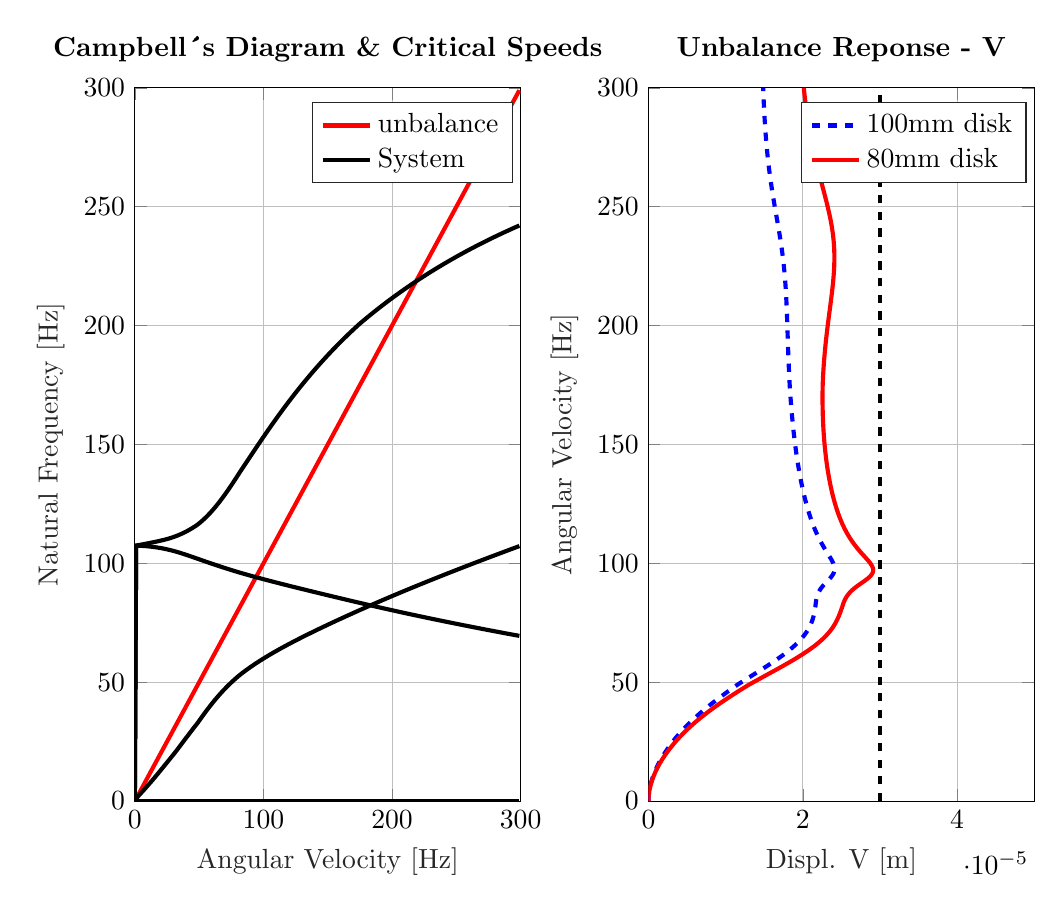
\begin{tikzpicture}

\begin{axis}[%
width=1.929in,
height=3.566in,
at={(0.777in,0.481in)},
scale only axis,
xmin=0,
xmax=300,
xlabel style={font=\color{white!15!black}},
xlabel={Angular Velocity [Hz]},
ymin=0,
ymax=300,
ylabel style={font=\color{white!15!black}},
ylabel={Natural Frequency [Hz]},
axis background/.style={fill=white},
title style={font=\bfseries},
title={Campbell´s Diagram \& Critical Speeds},
xmajorgrids,
ymajorgrids,
legend style={legend cell align=left, align=left, draw=white!15!black}
]
\addplot [color=red, line width=1.5pt]
  table[row sep=crcr]{%
0	0\\
1	1\\
2	2\\
3	3\\
4	4\\
5	5\\
6	6\\
7	7\\
8	8\\
9	9\\
10	10\\
11	11\\
12	12\\
13	13\\
14	14\\
15	15\\
16	16\\
17	17\\
18	18\\
19	19\\
20	20\\
21	21\\
22	22\\
23	23\\
24	24\\
25	25\\
26	26\\
27	27\\
28	28\\
29	29\\
30	30\\
31	31\\
32	32\\
33	33\\
34	34\\
35	35\\
36	36\\
37	37\\
38	38\\
39	39\\
40	40\\
41	41\\
42	42\\
43	43\\
44	44\\
45	45\\
46	46\\
47	47\\
48	48\\
49	49\\
50	50\\
51	51\\
52	52\\
53	53\\
54	54\\
55	55\\
56	56\\
57	57\\
58	58\\
59	59\\
60	60\\
61	61\\
62	62\\
63	63\\
64	64\\
65	65\\
66	66\\
67	67\\
68	68\\
69	69\\
70	70\\
71	71\\
72	72\\
73	73\\
74	74\\
75	75\\
76	76\\
77	77\\
78	78\\
79	79\\
80	80\\
81	81\\
82	82\\
83	83\\
84	84\\
85	85\\
86	86\\
87	87\\
88	88\\
89	89\\
90	90\\
91	91\\
92	92\\
93	93\\
94	94\\
95	95\\
96	96\\
97	97\\
98	98\\
99	99\\
100	100\\
101	101\\
102	102\\
103	103\\
104	104\\
105	105\\
106	106\\
107	107\\
108	108\\
109	109\\
110	110\\
111	111\\
112	112\\
113	113\\
114	114\\
115	115\\
116	116\\
117	117\\
118	118\\
119	119\\
120	120\\
121	121\\
122	122\\
123	123\\
124	124\\
125	125\\
126	126\\
127	127\\
128	128\\
129	129\\
130	130\\
131	131\\
132	132\\
133	133\\
134	134\\
135	135\\
136	136\\
137	137\\
138	138\\
139	139\\
140	140\\
141	141\\
142	142\\
143	143\\
144	144\\
145	145\\
146	146\\
147	147\\
148	148\\
149	149\\
150	150\\
151	151\\
152	152\\
153	153\\
154	154\\
155	155\\
156	156\\
157	157\\
158	158\\
159	159\\
160	160\\
161	161\\
162	162\\
163	163\\
164	164\\
165	165\\
166	166\\
167	167\\
168	168\\
169	169\\
170	170\\
171	171\\
172	172\\
173	173\\
174	174\\
175	175\\
176	176\\
177	177\\
178	178\\
179	179\\
180	180\\
181	181\\
182	182\\
183	183\\
184	184\\
185	185\\
186	186\\
187	187\\
188	188\\
189	189\\
190	190\\
191	191\\
192	192\\
193	193\\
194	194\\
195	195\\
196	196\\
197	197\\
198	198\\
199	199\\
200	200\\
201	201\\
202	202\\
203	203\\
204	204\\
205	205\\
206	206\\
207	207\\
208	208\\
209	209\\
210	210\\
211	211\\
212	212\\
213	213\\
214	214\\
215	215\\
216	216\\
217	217\\
218	218\\
219	219\\
220	220\\
221	221\\
222	222\\
223	223\\
224	224\\
225	225\\
226	226\\
227	227\\
228	228\\
229	229\\
230	230\\
231	231\\
232	232\\
233	233\\
234	234\\
235	235\\
236	236\\
237	237\\
238	238\\
239	239\\
240	240\\
241	241\\
242	242\\
243	243\\
244	244\\
245	245\\
246	246\\
247	247\\
248	248\\
249	249\\
250	250\\
251	251\\
252	252\\
253	253\\
254	254\\
255	255\\
256	256\\
257	257\\
258	258\\
259	259\\
260	260\\
261	261\\
262	262\\
263	263\\
264	264\\
265	265\\
266	266\\
267	267\\
268	268\\
269	269\\
270	270\\
271	271\\
272	272\\
273	273\\
274	274\\
275	275\\
276	276\\
277	277\\
278	278\\
279	279\\
280	280\\
281	281\\
282	282\\
283	283\\
284	284\\
285	285\\
286	286\\
287	287\\
288	288\\
289	289\\
290	290\\
291	291\\
292	292\\
293	293\\
294	294\\
295	295\\
296	296\\
297	297\\
298	298\\
299	299\\
};
\addlegendentry{unbalance}

\addplot [color=black, line width=1.5pt]
  table[row sep=crcr]{%
0	0\\
1	0\\
2	0\\
3	0\\
4	0\\
5	0\\
6	0\\
7	0\\
8	0\\
9	0\\
10	0\\
11	0\\
12	0\\
13	0\\
14	0\\
15	0\\
16	0\\
17	0\\
18	0\\
19	0\\
20	0\\
21	0\\
22	0\\
23	0\\
24	0\\
25	0\\
26	0\\
27	0\\
28	0\\
29	0\\
30	0\\
31	0\\
32	0\\
33	0\\
34	0\\
35	0\\
36	0\\
37	0\\
38	0\\
39	0\\
40	0\\
41	0\\
42	0\\
43	0\\
44	0\\
45	0\\
46	0\\
47	0\\
48	0\\
49	0\\
50	0\\
51	0\\
52	0\\
53	0\\
54	0\\
55	0\\
56	0\\
57	0\\
58	0\\
59	0\\
60	0\\
61	0\\
62	0\\
63	0\\
64	0\\
65	0\\
66	0\\
67	0\\
68	0\\
69	0\\
70	0\\
71	0\\
72	0\\
73	0\\
74	0\\
75	0\\
76	0\\
77	0\\
78	0\\
79	0\\
80	0\\
81	0\\
82	0\\
83	0\\
84	0\\
85	0\\
86	0\\
87	0\\
88	0\\
89	0\\
90	0\\
91	0\\
92	0\\
93	0\\
94	0\\
95	0\\
96	0\\
97	0\\
98	0\\
99	0\\
100	0\\
101	0\\
102	0\\
103	0\\
104	0\\
105	0\\
106	0\\
107	0\\
108	0\\
109	0\\
110	0\\
111	0\\
112	0\\
113	0\\
114	0\\
115	0\\
116	0\\
117	0\\
118	0\\
119	0\\
120	0\\
121	0\\
122	0\\
123	0\\
124	0\\
125	0\\
126	0\\
127	0\\
128	0\\
129	0\\
130	0\\
131	0\\
132	0\\
133	0\\
134	0\\
135	0\\
136	0\\
137	0\\
138	0\\
139	0\\
140	0\\
141	0\\
142	0\\
143	0\\
144	0\\
145	0\\
146	0\\
147	0\\
148	0\\
149	0\\
150	0\\
151	0\\
152	0\\
153	0\\
154	0\\
155	0\\
156	0\\
157	0\\
158	0\\
159	0\\
160	0\\
161	0\\
162	0\\
163	0\\
164	0\\
165	0\\
166	0\\
167	0\\
168	0\\
169	0\\
170	0\\
171	0\\
172	0\\
173	0\\
174	0\\
175	0\\
176	0\\
177	0\\
178	0\\
179	0\\
180	0\\
181	0\\
182	0\\
183	0\\
184	0\\
185	0\\
186	0\\
187	0\\
188	0\\
189	0\\
190	0\\
191	0\\
192	0\\
193	0\\
194	0\\
195	0\\
196	0\\
197	0\\
198	0\\
199	0\\
200	0\\
201	0\\
202	0\\
203	0\\
204	0\\
205	0\\
206	0\\
207	0\\
208	0\\
209	0\\
210	0\\
211	0\\
212	0\\
213	0\\
214	0\\
215	0\\
216	0\\
217	0\\
218	0\\
219	0\\
220	0\\
221	0\\
222	0\\
223	0\\
224	0\\
225	0\\
226	0\\
227	0\\
228	0\\
229	0\\
230	0\\
231	0\\
232	0\\
233	0\\
234	0\\
235	0\\
236	0\\
237	0\\
238	0\\
239	0\\
240	0\\
241	0\\
242	0\\
243	0\\
244	0\\
245	0\\
246	0\\
247	0\\
248	0\\
249	0\\
250	0\\
251	0\\
252	0\\
253	0\\
254	0\\
255	0\\
256	0\\
257	0\\
258	0\\
259	0\\
260	0\\
261	0\\
262	0\\
263	0\\
264	0\\
265	0\\
266	0\\
267	0\\
268	0\\
269	0\\
270	0\\
271	0\\
272	0\\
273	0\\
274	0\\
275	0\\
276	0\\
277	0\\
278	0\\
279	0\\
280	0\\
281	0\\
282	0\\
283	0\\
284	0\\
285	0\\
286	0\\
287	0\\
288	0\\
289	0\\
290	0\\
291	0\\
292	0\\
293	0\\
294	0\\
295	0\\
296	0\\
297	0\\
298	0\\
299	0\\
};
\addlegendentry{System}

\addplot [color=black, line width=1.5pt, forget plot]
  table[row sep=crcr]{%
0	0\\
1	0.874971235678326\\
2	1.65028234178887\\
3	2.29003417707735\\
4	2.90211216554813\\
5	3.49752599609471\\
6	4.08587592863577\\
7	4.66448336554673\\
8	5.2648752878829\\
9	5.88506694682445\\
10	6.50272881155821\\
11	7.11841170331159\\
12	7.73227894313637\\
13	8.35275038174122\\
14	8.99652621579654\\
15	9.64287859315492\\
16	10.2919983209097\\
17	10.9439796393002\\
18	11.5988248344515\\
19	12.2564478558825\\
20	12.9166777712831\\
21	13.5785713117566\\
22	14.2414574049218\\
23	14.9055644508479\\
24	15.5708652281663\\
25	16.2372873765126\\
26	16.9047165373701\\
27	17.5729999442359\\
28	18.2419496394459\\
29	18.9113428750971\\
30	19.5809276781827\\
31	20.2504220784664\\
32	20.9459482307154\\
33	21.6626562412702\\
34	22.3802835780286\\
35	23.0984761494743\\
36	23.8168618984701\\
37	24.5350529200253\\
38	25.2526466909656\\
39	25.9692267415315\\
40	26.6843658298727\\
41	27.3976266046195\\
42	28.1085651007425\\
43	28.8167310616445\\
44	29.521670677902\\
45	30.2229303730059\\
46	30.9200571060524\\
47	31.6126030621734\\
48	32.3001260700648\\
49	32.9965769598336\\
50	33.7666328773794\\
51	34.530473746824\\
52	35.2874221413458\\
53	36.0368293490531\\
54	36.7780815504769\\
55	37.5106064333073\\
56	38.2338733010946\\
57	38.947400723206\\
58	39.6507585861593\\
59	40.3435682287762\\
60	41.0255074070328\\
61	41.6963110206504\\
62	42.355764317333\\
63	43.0037110711102\\
64	43.6400475958616\\
65	44.2647174191144\\
66	44.8777161873039\\
67	45.4790801523487\\
68	46.0688886995667\\
69	46.647256161092\\
70	47.2143329277274\\
71	47.7702956409862\\
72	48.3153492380047\\
73	48.8497173577916\\
74	49.3736452092431\\
75	49.8873892794849\\
76	50.3912105711955\\
77	50.8853980740008\\
78	51.3702314523437\\
79	51.8459968376434\\
80	52.3129831074109\\
81	52.7714775492181\\
82	53.2114063561139\\
83	53.6318831903345\\
84	54.0457155280634\\
85	54.4531570998982\\
86	54.8544556946398\\
87	55.2498477475872\\
88	55.6395609152914\\
89	56.0238191054382\\
90	56.402832488164\\
91	56.7768070637616\\
92	57.1459383809535\\
93	57.5104141975662\\
94	57.8704157955585\\
95	58.2261168529434\\
96	58.5776829122139\\
97	58.9252748745487\\
98	59.2690418584976\\
99	59.6091333258985\\
100	59.9456866463015\\
101	60.278836908745\\
102	60.6087113782215\\
103	60.9354337694301\\
104	61.2591207174227\\
105	61.5798846811075\\
106	61.8978336037226\\
107	62.2130709924424\\
108	62.5256942590559\\
109	62.835799046335\\
110	63.1434756911398\\
111	63.4488117208134\\
112	63.7518899765025\\
113	64.0527908812874\\
114	64.3515900571127\\
115	64.6483624734165\\
116	64.9431782178254\\
117	65.236104672285\\
118	65.527208303802\\
119	65.8165492324286\\
120	66.1041899993393\\
121	66.3901867978064\\
122	66.6745961897116\\
123	66.9574708956231\\
124	67.2388620574515\\
125	67.5188210448238\\
126	67.7973927713324\\
127	68.0746238668184\\
128	68.350557819417\\
129	68.6252379001533\\
130	68.8987037388456\\
131	69.1709938007465\\
132	69.4421461\\
133	69.712196750918\\
134	69.9811803183804\\
135	70.249129593971\\
136	70.5160757746199\\
137	70.7820493311958\\
138	71.0470795401074\\
139	71.3111935625834\\
140	71.5744193425002\\
141	71.8367802986837\\
142	72.0983000742772\\
143	72.3590041853098\\
144	72.6189092985473\\
145	72.878040174709\\
146	73.136414344701\\
147	73.394053249129\\
148	73.6509657636732\\
149	73.9071767171253\\
150	74.1626938137736\\
151	74.417537960681\\
152	74.6717161742831\\
153	74.9252424128807\\
154	75.1781286317722\\
155	75.430384522173\\
156	75.6820198814565\\
157	75.9330425358877\\
158	76.1834586326292\\
159	76.4332764961505\\
160	76.6825048607542\\
161	76.9311477289735\\
162	77.1792088267549\\
163	77.4266924568041\\
164	77.6736043356203\\
165	77.9199486610357\\
166	78.1657269361672\\
167	78.4109442633865\\
168	78.6556016125088\\
169	78.8997030952633\\
170	79.143247684255\\
171	79.3862387959495\\
172	79.6286774182963\\
173	79.8705721184434\\
174	80.1119173903067\\
175	80.3527760644489\\
176	80.593205698259\\
177	80.8331622454144\\
178	81.0726483980372\\
179	81.311661649621\\
180	81.5501980901488\\
181	81.7882610256689\\
182	82.0258503013461\\
183	82.2629611127702\\
184	82.2246976940528\\
185	82.1004960975746\\
186	81.9765436243732\\
187	81.8528481580071\\
188	81.729420118185\\
189	81.606244602735\\
190	81.4833288527217\\
191	81.3606777433785\\
192	81.2382927817483\\
193	81.1161689104734\\
194	80.9943132321542\\
195	80.8727266611065\\
196	80.7514101634066\\
197	80.6303644806269\\
198	80.5095781013566\\
199	80.3890680215667\\
200	80.2688170228538\\
201	80.14883301285\\
202	80.0291165600196\\
203	79.9096707148795\\
204	79.7904843618206\\
205	79.671558284838\\
206	79.5528940283344\\
207	79.434500824243\\
208	79.3163540873091\\
209	79.1984701362982\\
210	79.0808426920816\\
211	78.9634761464361\\
212	78.846352992154\\
213	78.7294843694103\\
214	78.6128691439155\\
215	78.4965002973703\\
216	78.3803721997643\\
217	78.2645002068745\\
218	78.1488599263504\\
219	78.0334757710933\\
220	77.9183252686202\\
221	77.8034123429967\\
222	77.6887310033188\\
223	77.574290138813\\
224	77.4600835254443\\
225	77.3461095564699\\
226	77.2323655640607\\
227	77.1188490012141\\
228	77.0055636158265\\
229	76.8924990396833\\
230	76.7796680846399\\
231	76.6670544331906\\
232	76.5546663108671\\
233	76.4424903153601\\
234	76.3305373708341\\
235	76.2188070192804\\
236	76.1072834618601\\
237	75.99598725353\\
238	75.884893213376\\
239	75.7740274610102\\
240	75.6633617566415\\
241	75.5529139550454\\
242	75.4426644565845\\
243	75.3326330494156\\
244	75.2228133010081\\
245	75.113188710028\\
246	75.0037794725985\\
247	74.8945749766065\\
248	74.7855642479056\\
249	74.6767685957737\\
250	74.5681653698277\\
251	74.4597688301189\\
252	74.3515752395572\\
253	74.2435811493815\\
254	74.1357825665933\\
255	74.0281838955838\\
256	73.9207803050883\\
257	73.8135805422962\\
258	73.7065740360517\\
259	73.5997658614502\\
260	73.4931469508739\\
261	73.3867237033657\\
262	73.2804913537815\\
263	73.1744624334474\\
264	73.0686206866147\\
265	72.9629718287934\\
266	72.857513064703\\
267	72.7522424327762\\
268	72.6471719911193\\
269	72.5422900337659\\
270	72.43759266349\\
271	72.3330907330171\\
272	72.228775064032\\
273	72.1246456303719\\
274	72.0207100861059\\
275	71.9169553321222\\
276	71.8133957082014\\
277	71.71002347392\\
278	71.6068301617355\\
279	71.5038284880118\\
280	71.4010099054537\\
281	71.2983796158417\\
282	71.1959361648195\\
283	71.0936773797552\\
284	70.9915996065137\\
285	70.889708821151\\
286	70.7880038149882\\
287	70.6864831932118\\
288	70.5851449138499\\
289	70.4839878334988\\
290	70.38301475327\\
291	70.2822263862518\\
292	70.1816192206949\\
293	70.081194662031\\
294	69.9809567712123\\
295	69.8808938253025\\
296	69.7810117567439\\
297	69.6813208937371\\
298	69.581805426246\\
299	69.4824660045069\\
};
\addplot [color=black, line width=1.5pt, forget plot]
  table[row sep=crcr]{%
0	0\\
1	107.406805161813\\
2	107.397589804316\\
3	107.38327630972\\
4	107.363987582276\\
5	107.340650404373\\
6	107.312989988406\\
7	107.281284706434\\
8	107.244138171917\\
9	107.201285512702\\
10	107.1539039473\\
11	107.102161793738\\
12	107.046239738925\\
13	106.985847771243\\
14	106.919865486159\\
15	106.849315462609\\
16	106.774244646795\\
17	106.69468355488\\
18	106.610676059192\\
19	106.522265469744\\
20	106.4294945806\\
21	106.330622069012\\
22	106.225981033169\\
23	106.116541401448\\
24	106.002337307745\\
25	105.883431793869\\
26	105.759902100817\\
27	105.631837262856\\
28	105.499356381336\\
29	105.362573143114\\
30	105.221636106733\\
31	105.076700904002\\
32	104.924894092617\\
33	104.766753263646\\
34	104.604753001115\\
35	104.439123672906\\
36	104.270110550111\\
37	104.097975507432\\
38	103.922976586632\\
39	103.745374953051\\
40	103.565436865955\\
41	103.383421141548\\
42	103.199590954223\\
43	103.014197216567\\
44	102.827473563143\\
45	102.639661411305\\
46	102.450972945906\\
47	102.261621280615\\
48	102.071790900172\\
49	101.881749481352\\
50	101.692069640573\\
51	101.50253945543\\
52	101.313283815452\\
53	101.124408957826\\
54	100.936020783143\\
55	100.748211630114\\
56	100.561056427997\\
57	100.374623311088\\
58	100.188983645416\\
59	100.004171142395\\
60	99.8202425074528\\
61	99.6372377453624\\
62	99.4551799395959\\
63	99.2741021247057\\
64	99.0940199667411\\
65	98.9149514930112\\
66	98.7369091132477\\
67	98.5599035279277\\
68	98.3839365699301\\
69	98.2090145888631\\
70	98.0351341760411\\
71	97.8622956976233\\
72	97.6904909955505\\
73	97.5197131675484\\
74	97.3499519929102\\
75	97.1812132592794\\
76	97.0134735545946\\
77	96.8467241324884\\
78	96.6809442374607\\
79	96.5161390449857\\
80	96.352281498789\\
81	96.1893647259657\\
82	96.0294652193923\\
83	95.872953149955\\
84	95.7173370505758\\
85	95.5625960219751\\
86	95.4087041811349\\
87	95.2556404469075\\
88	95.1033821435004\\
89	94.9519123078428\\
90	94.8012049076441\\
91	94.6512369609839\\
92	94.50199117552\\
93	94.3534506271905\\
94	94.2055896804913\\
95	94.0583936166039\\
96	93.9118432230243\\
97	93.7659163830878\\
98	93.62060113165\\
99	93.4758757584545\\
100	93.331729301577\\
101	93.1881389135417\\
102	93.0450872098825\\
103	92.9025635039387\\
104	92.7605455723391\\
105	92.6190288725217\\
106	92.4779904201492\\
107	92.3374151531754\\
108	92.1972926742415\\
109	92.0576086283796\\
110	91.9183466010284\\
111	91.7794942459478\\
112	91.6410378427241\\
113	91.5029634350833\\
114	91.3652649044511\\
115	91.2279193254945\\
116	91.0909266262641\\
117	90.9542628993366\\
118	90.8179239636487\\
119	90.6818996741034\\
120	90.5461727025086\\
121	90.4107382927456\\
122	90.2755778065945\\
123	90.1406882942629\\
124	90.0060580484404\\
125	89.871671639673\\
126	89.7375263496846\\
127	89.6036091845198\\
128	89.4699112243511\\
129	89.3364241197363\\
130	89.2031380249837\\
131	89.0700490129288\\
132	88.9371446128117\\
133	88.8044167877677\\
134	88.6718626532602\\
135	88.5394713478994\\
136	88.4072361629258\\
137	88.2751515949533\\
138	88.1432132758276\\
139	88.0114224392963\\
140	87.8797510096138\\
141	87.7482206317219\\
142	87.6168184501182\\
143	87.4855394475982\\
144	87.3543785374832\\
145	87.2233328094276\\
146	87.0924134820546\\
147	86.9615885857729\\
148	86.8308948660143\\
149	86.7003084243912\\
150	86.5698344765754\\
151	86.4394658817929\\
152	86.3092269023702\\
153	86.1790932565008\\
154	86.0490847893578\\
155	85.9191880369986\\
156	85.7894209899142\\
157	85.6597686968738\\
158	85.5302612243312\\
159	85.4008866664162\\
160	85.2716451396519\\
161	85.1425448638193\\
162	85.0135890144358\\
163	84.8847979805932\\
164	84.7561662534641\\
165	84.6276915946072\\
166	84.499387881047\\
167	84.3712547907969\\
168	84.2433099870805\\
169	84.1155458020941\\
170	83.9879775505884\\
171	83.860613436112\\
172	83.7334506751925\\
173	83.6064892945436\\
174	83.4797438673752\\
175	83.353227416285\\
176	83.2269391087109\\
177	83.1008649913361\\
178	82.9749997326409\\
179	82.8493664738399\\
180	82.7239570981312\\
181	82.5987788159368\\
182	82.4738369121576\\
183	82.3491431721571\\
184	82.4995975114542\\
185	82.7357599793743\\
186	82.9714487359736\\
187	83.2066646981587\\
188	83.4414040717418\\
189	83.6756743625754\\
190	83.9094780754288\\
191	84.1428115899759\\
192	84.3756814202394\\
193	84.6080899433121\\
194	84.8400351372031\\
195	85.0715199736719\\
196	85.3025481849178\\
197	85.5331253601183\\
198	85.7632541727655\\
199	85.9929342818708\\
200	86.2221688541459\\
201	86.4509668064684\\
202	86.6793257182842\\
203	86.9072503596821\\
204	87.1347463949298\\
205	87.361818855648\\
206	87.5884671603202\\
207	87.814693241934\\
208	88.0405071429826\\
209	88.2659089210155\\
210	88.4909059826409\\
211	88.7154934315393\\
212	88.9396886115041\\
213	89.1634846593095\\
214	89.3868883752269\\
215	89.6099020806981\\
216	89.8325342562156\\
217	90.0547809493271\\
218	90.2766551405118\\
219	90.498151464183\\
220	90.7192823262608\\
221	90.9400407274587\\
222	91.1604404173782\\
223	91.3804796072083\\
224	91.6001613094644\\
225	91.8194949766663\\
226	92.0384726809826\\
227	92.2571095218017\\
228	92.475400897673\\
229	92.693350179102\\
230	92.9109668278794\\
231	93.1282463129411\\
232	93.3451966262433\\
233	93.5618190044285\\
234	93.7781185621439\\
235	93.9940906937967\\
236	94.2097497694778\\
237	94.4250855825205\\
238	94.6401121111834\\
239	94.8548215793602\\
240	95.0692276356609\\
241	95.2833245940848\\
242	95.4971200124144\\
243	95.7106110047248\\
244	95.9238007693269\\
245	96.136696918209\\
246	96.3492955807543\\
247	96.5616023844129\\
248	96.7736207350613\\
249	96.9853447365024\\
250	97.1967910011334\\
251	97.4079445399229\\
252	97.6188154847172\\
253	97.8294059069494\\
254	98.0397235168008\\
255	98.2497573755157\\
256	98.459521738866\\
257	98.6690035826204\\
258	98.8782198553571\\
259	99.0871620850204\\
260	99.2958388021641\\
261	99.5042482422782\\
262	99.7123949437628\\
263	99.9202729705853\\
264	100.127889347403\\
265	100.335243087931\\
266	100.542338737003\\
267	100.749177073527\\
268	100.955757452795\\
269	101.162083596599\\
270	101.368151417156\\
271	101.573971695741\\
272	101.77953644811\\
273	101.984851088003\\
274	102.189918337662\\
275	102.394739028217\\
276	102.599310555856\\
277	102.803634868969\\
278	103.007715916049\\
279	103.211553705675\\
280	103.415146884398\\
281	103.618503979853\\
282	103.82161399704\\
283	104.024489623313\\
284	104.227125409269\\
285	104.429520279727\\
286	104.631683893889\\
287	104.833606964615\\
288	105.03530138376\\
289	105.23675833222\\
290	105.437985377882\\
291	105.638972188997\\
292	105.839734685599\\
293	106.040265558746\\
294	106.240567947614\\
295	106.440648727792\\
296	106.640491923577\\
297	106.840106504677\\
298	107.039496287743\\
299	107.238667656429\\
};
\addplot [color=black, line width=1.5pt, forget plot]
  table[row sep=crcr]{%
0	0\\
1	107.473294103906\\
2	107.574980911479\\
3	107.677494965992\\
4	107.780822471265\\
5	107.88189904721\\
6	107.983266415924\\
7	108.084272581532\\
8	108.190576033492\\
9	108.297392183312\\
10	108.403283265453\\
11	108.509410769961\\
12	108.617157293604\\
13	108.726510803889\\
14	108.833943775075\\
15	108.943190499153\\
16	109.055069210575\\
17	109.170414109815\\
18	109.29007463738\\
19	109.414897092724\\
20	109.545776949552\\
21	109.671753337529\\
22	109.796921759449\\
23	109.928238238032\\
24	110.066171668789\\
25	110.211186834715\\
26	110.363680461532\\
27	110.524047261735\\
28	110.692683070704\\
29	110.869888255038\\
30	111.056031824317\\
31	111.251407338124\\
32	111.454516284575\\
33	111.66538224855\\
34	111.885373768123\\
35	112.114673845776\\
36	112.353420967238\\
37	112.601752816223\\
38	112.859830956495\\
39	113.127763211389\\
40	113.405679403629\\
41	113.693706307707\\
42	113.991975494327\\
43	114.300599936008\\
44	114.61972464021\\
45	114.949459758467\\
46	115.289926735415\\
47	115.641276501182\\
48	116.003609929025\\
49	116.3844864339\\
50	116.820014881272\\
51	117.271176227857\\
52	117.738269475841\\
53	118.221536968492\\
54	118.72122531913\\
55	119.237493183481\\
56	119.770465271588\\
57	120.320212078629\\
58	120.886760566123\\
59	121.470042904367\\
60	122.069989218894\\
61	122.686394381153\\
62	123.319073109879\\
63	123.967736420068\\
64	124.632019469772\\
65	125.311573116527\\
66	126.00592297718\\
67	126.714613281026\\
68	127.437086131707\\
69	128.17283595322\\
70	128.921214923063\\
71	129.681661008085\\
72	130.453492604371\\
73	131.236080208799\\
74	132.028765750609\\
75	132.830853802631\\
76	133.641727227253\\
77	134.460655322766\\
78	135.286978992206\\
79	136.120062076654\\
80	136.959243008898\\
81	137.803910126356\\
82	138.633927631452\\
83	139.443536266893\\
84	140.254780252349\\
85	141.067269030276\\
86	141.880552187356\\
87	142.694265861102\\
88	143.508109163431\\
89	144.3216718601\\
90	145.134653691336\\
91	145.946724397451\\
92	146.757599400658\\
93	147.567038846842\\
94	148.374771076926\\
95	149.180531696946\\
96	149.984112937539\\
97	150.785274785508\\
98	151.58389342693\\
99	152.379682167082\\
100	153.172549677341\\
101	153.962304331699\\
102	154.748790953851\\
103	155.531882712002\\
104	156.311436501955\\
105	157.08737174656\\
106	157.859553171744\\
107	158.627883850797\\
108	159.392288752298\\
109	160.152691595636\\
110	160.908989870718\\
111	161.661135835026\\
112	162.409073298255\\
113	163.152719218086\\
114	163.892098496255\\
115	164.627069400533\\
116	165.357666899146\\
117	166.083841064999\\
118	166.805532633549\\
119	167.522793680922\\
120	168.235534606193\\
121	168.943804359005\\
122	169.647532838435\\
123	170.346737385524\\
124	171.041443456526\\
125	171.731557876299\\
126	172.417175893935\\
127	173.098270196268\\
128	173.774860273428\\
129	174.446911424496\\
130	175.114464123412\\
131	175.777555203701\\
132	176.4361635607\\
133	177.090320953165\\
134	177.740020509849\\
135	178.385293902799\\
136	179.026176390868\\
137	179.662678515987\\
138	180.294817019304\\
139	180.922635114408\\
140	181.546062069348\\
141	182.16528237205\\
142	182.780236215082\\
143	183.390904523004\\
144	183.997371256433\\
145	184.599683233635\\
146	185.19786299681\\
147	185.791763817937\\
148	186.38172611371\\
149	186.967522238666\\
150	187.549314838202\\
151	188.127038962957\\
152	188.700838791251\\
153	189.270615016038\\
154	189.836544106708\\
155	190.398511382292\\
156	190.956596589519\\
157	191.510817242782\\
158	192.061312175872\\
159	192.608011627812\\
160	193.150918046199\\
161	193.690054029698\\
162	194.225545848501\\
163	194.757424035883\\
164	195.285654565507\\
165	195.810265671666\\
166	196.331280219399\\
167	196.848721676973\\
168	197.362685954744\\
169	197.87307807145\\
170	198.380112117835\\
171	198.883705164886\\
172	199.383926025762\\
173	199.880666952704\\
174	200.374050570655\\
175	200.849880602571\\
176	201.308192236029\\
177	201.763911939734\\
178	202.216931318281\\
179	202.667368747792\\
180	203.115261657687\\
181	203.560562562571\\
182	204.003265659598\\
183	204.443517340955\\
184	204.881301347771\\
185	205.316534486292\\
186	205.749250172523\\
187	206.179516208456\\
188	206.607452013988\\
189	207.032886800928\\
190	207.455873871063\\
191	207.876498933328\\
192	208.294715817003\\
193	208.710484451327\\
194	209.123982082306\\
195	209.535138715455\\
196	209.944000590572\\
197	210.350545959037\\
198	210.75474863429\\
199	211.156724945335\\
200	211.55637879921\\
201	211.953792076771\\
202	212.348985392656\\
203	212.742015474269\\
204	213.132793851173\\
205	213.52131465042\\
206	213.907692520385\\
207	214.292023361138\\
208	214.674056006987\\
209	215.054061292272\\
210	215.431874639359\\
211	215.807706940317\\
212	216.181285982226\\
213	216.552847284437\\
214	216.922379266738\\
215	217.289857457898\\
216	217.655207133186\\
217	218.018668158465\\
218	218.379998694936\\
219	218.739464824059\\
220	219.096874382526\\
221	219.452339808987\\
222	219.805805560564\\
223	220.157323328978\\
224	220.506980283672\\
225	220.854670326977\\
226	221.200510749375\\
227	221.544415734049\\
228	221.886467163901\\
229	222.226646699945\\
230	222.565006606376\\
231	222.901553467629\\
232	223.236229791854\\
233	223.56907807637\\
234	223.900105981106\\
235	224.229442555465\\
236	224.55688781852\\
237	224.882678421051\\
238	225.206633610789\\
239	225.52896499979\\
240	225.849477162884\\
241	226.168316062651\\
242	226.485357818184\\
243	226.800819156005\\
244	227.114646521585\\
245	227.426681950969\\
246	227.737135725918\\
247	228.045965897999\\
248	228.353087223076\\
249	228.658678078837\\
250	228.962535944072\\
251	229.264910272022\\
252	229.565706349428\\
253	229.864923875705\\
254	230.162512469022\\
255	230.458629941365\\
256	230.753120644747\\
257	231.046193195456\\
258	231.337680167242\\
259	231.627725590281\\
260	231.916194149643\\
261	232.203185805865\\
262	232.488654311966\\
263	232.77279283461\\
264	233.055434197934\\
265	233.33658873553\\
266	233.616350573647\\
267	233.894623039736\\
268	234.171574010409\\
269	234.447132984997\\
270	234.721242663667\\
271	234.993997560017\\
272	235.265377919508\\
273	235.535380670954\\
274	235.804065625868\\
275	236.071371146208\\
276	236.337414554582\\
277	236.602114815809\\
278	236.865439730607\\
279	237.127519800893\\
280	237.388274712091\\
281	237.647773647253\\
282	237.906012212928\\
283	238.16298004698\\
284	238.418649990758\\
285	238.673118763934\\
286	238.926369031509\\
287	239.178415680613\\
288	239.429164495322\\
289	239.678726970931\\
290	239.927067820581\\
291	240.174275751367\\
292	240.420272218437\\
293	240.665115430512\\
294	240.908804283742\\
295	241.151268919907\\
296	241.392591057997\\
297	241.632894014791\\
298	241.872006737969\\
299	242.109907045657\\
};
\end{axis}

\begin{axis}[%
width=1.929in,
height=3.566in,
at={(3.345in,0.481in)},
scale only axis,
xmin=0,
xmax=5e-05,
xlabel style={font=\color{white!15!black}},
xlabel={Displ. V [m]},
ymin=0,
ymax=300,
ylabel style={font=\color{white!15!black}},
ylabel={Angular Velocity [Hz]},
axis background/.style={fill=white},
title style={font=\bfseries},
title={Unbalance Reponse - V},
xmajorgrids,
ymajorgrids,
legend style={legend cell align=left, align=left, draw=white!15!black}
]
\addplot [color=blue, dashed, line width=1.5pt]
  table[row sep=crcr]{%
0	0\\
5.68742446831822e-10	0.3\\
2.22149003769155e-09	0.6\\
4.95634561659305e-09	0.9\\
9.10415279399603e-09	1.2\\
1.42749064960762e-08	1.5\\
2.04380736867539e-08	1.8\\
2.77888994573599e-08	2.1\\
3.62426361657711e-08	2.4\\
4.54333991895716e-08	2.7\\
5.56471491828436e-08	3\\
6.69174726803994e-08	3.3\\
7.92957876183908e-08	3.6\\
9.25403567113165e-08	3.9\\
1.06736579510498e-07	4.2\\
1.21940592058567e-07	4.5\\
1.38173062532252e-07	4.8\\
1.55460906688741e-07	5.1\\
1.7368512292356e-07	5.4\\
1.92499123901877e-07	5.7\\
2.12246890147687e-07	6\\
2.32936818876024e-07	6.3\\
2.54579782630535e-07	6.6\\
2.77189129420699e-07	6.9\\
3.00780682203485e-07	7.2\\
3.25006901070921e-07	7.5\\
3.49665658227703e-07	7.8\\
3.75166784177616e-07	8.1\\
4.01513021593643e-07	8.4\\
4.28708172005332e-07	8.7\\
4.56757077110127e-07	9\\
4.85665602277501e-07	9.3\\
5.15440622050408e-07	9.6\\
5.46090007446188e-07	9.9\\
5.77622614869579e-07	10.2\\
6.1004827642229e-07	10.5\\
6.43377791436837e-07	10.8\\
6.77622918963878e-07	11.1\\
7.12796371036056e-07	11.4\\
7.48911806427579e-07	11.7\\
7.85983824674297e-07	12\\
8.24027960066938e-07	12.3\\
8.63060675295291e-07	12.6\\
9.02302320831105e-07	12.9\\
9.41846113320911e-07	13.2\\
9.82215348151603e-07	13.5\\
1.02341443754289e-06	13.8\\
1.06544813837865e-06	14.1\\
1.10832154139436e-06	14.4\\
1.15204006064655e-06	14.7\\
1.19660942315941e-06	15\\
1.24203565876036e-06	15.3\\
1.28832509002794e-06	15.6\\
1.33548432233017e-06	15.9\\
1.38352023390338e-06	16.2\\
1.43243996592146e-06	16.5\\
1.4822509125481e-06	16.8\\
1.53296071087251e-06	17.1\\
1.5845772307556e-06	17.4\\
1.63710856448093e-06	17.7\\
1.69056301622259e-06	18\\
1.74494909123548e-06	18.3\\
1.80027548475372e-06	18.6\\
1.85655107057431e-06	18.9\\
1.91378488923854e-06	19.2\\
1.97198613574264e-06	19.5\\
2.03116414686591e-06	19.8\\
2.0913283878709e-06	20.1\\
2.15218518833012e-06	20.4\\
2.21157277119969e-06	20.7\\
2.2717655683088e-06	21\\
2.33276666022028e-06	21.3\\
2.39457916855522e-06	21.6\\
2.45720624760088e-06	21.9\\
2.52065107590256e-06	22.2\\
2.58491684772365e-06	22.5\\
2.65000676443512e-06	22.8\\
2.71592402578766e-06	23.1\\
2.78267182106942e-06	23.4\\
2.85025332010094e-06	23.7\\
2.91867166418848e-06	24\\
2.98792995677342e-06	24.3\\
3.05803125407665e-06	24.6\\
3.12897855548865e-06	24.9\\
3.2007747938127e-06	25.2\\
3.27342282530326e-06	25.5\\
3.3469254195443e-06	25.8\\
3.42128524912242e-06	26.1\\
3.49650487905194e-06	26.4\\
3.57258675607346e-06	26.7\\
3.64953319765707e-06	27\\
3.72734638082516e-06	27.3\\
3.8060283307285e-06	27.6\\
3.88558090905477e-06	27.9\\
3.96600580207613e-06	28.2\\
4.04730450862848e-06	28.5\\
4.1294783277241e-06	28.8\\
4.21252834598755e-06	29.1\\
4.29645542486176e-06	29.4\\
4.38126018755979e-06	29.7\\
4.46694300579984e-06	30\\
4.55350398630259e-06	30.3\\
4.64094295709694e-06	30.6\\
4.72925945354568e-06	30.9\\
4.81845270428641e-06	31.2\\
4.90848566156817e-06	31.5\\
4.99927508168127e-06	31.8\\
5.09095942149316e-06	32.1\\
5.18353930983244e-06	32.4\\
5.27701513620844e-06	32.7\\
5.37138703877079e-06	33\\
5.46665489204977e-06	33.3\\
5.56281829454896e-06	33.6\\
5.65987655600709e-06	33.9\\
5.75782868453204e-06	34.2\\
5.85667337357708e-06	34.5\\
5.95640898862518e-06	34.8\\
6.05703355380047e-06	35.1\\
6.15854473824636e-06	35.4\\
6.2609398423686e-06	35.7\\
6.36421578397658e-06	36\\
6.46836908418775e-06	36.3\\
6.57339585337037e-06	36.6\\
6.67929177689057e-06	36.9\\
6.78605210080403e-06	37.2\\
6.89367161751913e-06	37.5\\
7.00214465140882e-06	37.8\\
7.11146504444427e-06	38.1\\
7.22162614176763e-06	38.4\\
7.33262077744472e-06	38.7\\
7.44444126017229e-06	39\\
7.55707935909671e-06	39.3\\
7.6705262899301e-06	39.6\\
7.78477270096931e-06	39.9\\
7.8998086595431e-06	40.2\\
8.01562363865135e-06	40.5\\
8.1322065038414e-06	40.8\\
8.24954550043871e-06	41.1\\
8.36762824111005e-06	41.4\\
8.48644169397706e-06	41.7\\
8.60597217097367e-06	42\\
8.72620531688304e-06	42.3\\
8.84712609888829e-06	42.6\\
8.96871879664096e-06	42.9\\
9.09096699312572e-06	43.2\\
9.21385356611278e-06	43.5\\
9.3373606804874e-06	43.8\\
9.46146978123821e-06	44.1\\
9.58616158747995e-06	44.4\\
9.71141608733788e-06	44.7\\
9.83721253373807e-06	45\\
9.96352944137822e-06	45.3\\
1.00903445846414e-05	45.6\\
1.021763499679e-05	45.9\\
1.03453769702518e-05	46.2\\
1.04735460582185e-05	46.5\\
1.06021170774959e-05	46.8\\
1.07310641127726e-05	47.1\\
1.08603605222771e-05	47.4\\
1.09899789447266e-05	47.7\\
1.11198913080697e-05	48\\
1.12500688394091e-05	48.3\\
1.13804820767499e-05	48.6\\
1.1513495413408e-05	48.9\\
1.16579173968967e-05	49.2\\
1.18028152011607e-05	49.5\\
1.19481528785795e-05	49.8\\
1.20938933019003e-05	50.1\\
1.22399981733233e-05	50.4\\
1.23864280361472e-05	50.7\\
1.2533142289541e-05	51\\
1.26800992063275e-05	51.3\\
1.28272559539818e-05	51.6\\
1.29745686188226e-05	51.9\\
1.31219922336584e-05	52.2\\
1.32694808085329e-05	52.5\\
1.34169873652925e-05	52.8\\
1.35644639753708e-05	53.1\\
1.37118618010435e-05	53.4\\
1.38591311404738e-05	53.7\\
1.40062214758969e-05	54\\
1.41530815256171e-05	54.3\\
1.42996592992348e-05	54.6\\
1.44459021563855e-05	54.9\\
1.45917568687442e-05	55.2\\
1.4737169685251e-05	55.5\\
1.48820864006046e-05	55.8\\
1.50264524265089e-05	56.1\\
1.51702128659902e-05	56.4\\
1.5313312590274e-05	56.7\\
1.54556963182144e-05	57\\
1.55973086979687e-05	57.3\\
1.57380943908724e-05	57.6\\
1.58779981570769e-05	57.9\\
1.60169649427795e-05	58.2\\
1.61549399688101e-05	58.5\\
1.6291868820314e-05	58.8\\
1.64276975371686e-05	59.1\\
1.6562372704875e-05	59.4\\
1.66958415456947e-05	59.7\\
1.68280520094406e-05	60\\
1.69589528640634e-05	60.3\\
1.70884937853008e-05	60.6\\
1.72166254452488e-05	60.9\\
1.734329959948e-05	61.2\\
1.74684691726072e-05	61.5\\
1.75920883415126e-05	61.8\\
1.77141126165207e-05	62.1\\
1.78344989197748e-05	62.4\\
1.79532056607496e-05	62.7\\
1.80701928086697e-05	63\\
1.81854219613843e-05	63.3\\
1.82988564108402e-05	63.6\\
1.84104612043978e-05	63.9\\
1.85202032025008e-05	64.2\\
1.86280511319209e-05	64.5\\
1.8733975634871e-05	64.8\\
1.88379493134989e-05	65.1\\
1.8939946770279e-05	65.4\\
1.90399446433835e-05	65.7\\
1.91379216380341e-05	66\\
1.92338585528792e-05	66.3\\
1.93277383021739e-05	66.6\\
1.94195459333461e-05	66.9\\
1.9509268640352e-05	67.2\\
1.95968957727266e-05	67.5\\
1.96824188407829e-05	67.8\\
1.97658315165107e-05	68.1\\
1.98471296313847e-05	68.4\\
1.99263111703386e-05	68.7\\
2.00033762627266e-05	69\\
2.00783271702726e-05	69.3\\
2.01511682727493e-05	69.6\\
2.02219060510351e-05	69.9\\
2.02905490684495e-05	70.2\\
2.03571079507653e-05	70.5\\
2.04215953646714e-05	70.8\\
2.04840259957732e-05	71.1\\
2.05444165263609e-05	71.4\\
2.06027856129953e-05	71.7\\
2.06591538650572e-05	72\\
2.07135438241431e-05	72.3\\
2.07659799450119e-05	72.6\\
2.08164885786061e-05	72.9\\
2.08650979577762e-05	73.2\\
2.09118381858821e-05	73.5\\
2.09567412291534e-05	73.8\\
2.09998409132264e-05	74.1\\
2.1041172924371e-05	74.4\\
2.10807748161202e-05	74.7\\
2.11186860217714e-05	75\\
2.11549478734769e-05	75.3\\
2.11896036284878e-05	75.6\\
2.12226985029178e-05	75.9\\
2.12542797142387e-05	76.2\\
2.12843965326558e-05	76.5\\
2.1313100342069e-05	76.8\\
2.13404447112636e-05	77.1\\
2.13664854762746e-05	77.4\\
2.13912808338096e-05	77.7\\
2.14148914470513e-05	78\\
2.14373805636077e-05	78.3\\
2.14588141468076e-05	78.6\\
2.1479261019684e-05	78.9\\
2.14987930229682e-05	79.2\\
2.15174851860644e-05	79.5\\
2.15354159116532e-05	79.8\\
2.15526671727273e-05	80.1\\
2.15693247220293e-05	80.4\\
2.15854783118807e-05	80.7\\
2.1601221923485e-05	81\\
2.16166540026084e-05	81.3\\
2.16305828763909e-05	81.6\\
2.16391367690586e-05	81.9\\
2.16479551328357e-05	82.2\\
2.1657163488152e-05	82.5\\
2.16668932679869e-05	82.8\\
2.16772820352962e-05	83.1\\
2.16884736600386e-05	83.4\\
2.17006184409574e-05	83.7\\
2.17138731550225e-05	84\\
2.17284010143593e-05	84.3\\
2.17443715058993e-05	84.6\\
2.17619600875155e-05	84.9\\
2.17813477077931e-05	85.2\\
2.18027201154029e-05	85.5\\
2.18262669177902e-05	85.8\\
2.18521803473633e-05	86.1\\
2.18806536894241e-05	86.4\\
2.19118793252597e-05	86.7\\
2.19460463440291e-05	87\\
2.1983337679192e-05	87.3\\
2.20239267320279e-05	87.6\\
2.2067973454344e-05	87.9\\
2.2115619877732e-05	88.2\\
2.21669850972949e-05	88.5\\
2.22221597465162e-05	88.8\\
2.22812000333879e-05	89.1\\
2.23441214504287e-05	89.4\\
2.2410892318831e-05	89.7\\
2.24814273794591e-05	90\\
2.2555581696793e-05	90.3\\
2.26331451941672e-05	90.6\\
2.27138381805694e-05	90.9\\
2.27973082590491e-05	91.2\\
2.28831290134916e-05	91.5\\
2.29708008485796e-05	91.8\\
2.30597543039584e-05	92.1\\
2.31493560690857e-05	92.4\\
2.32389177974334e-05	92.7\\
2.33277076575589e-05	93\\
2.34149643750246e-05	93.3\\
2.34999133325906e-05	93.6\\
2.35817841169065e-05	93.9\\
2.36598287575467e-05	94.2\\
2.37333398080163e-05	94.5\\
2.38016673891716e-05	94.8\\
2.38642343560219e-05	95.1\\
2.39205488605584e-05	95.4\\
2.39702137531425e-05	95.7\\
2.40129324770255e-05	96\\
2.40485113435572e-05	96.3\\
2.40768583023969e-05	96.6\\
2.40979785221172e-05	96.9\\
2.41119672577619e-05	97.2\\
2.4119000585828e-05	97.5\\
2.41193246397146e-05	97.8\\
2.41132439766169e-05	98.1\\
2.41011096619671e-05	98.4\\
2.40833075808859e-05	98.7\\
2.40602473896781e-05	99\\
2.4032352415216e-05	99.3\\
2.40000507078446e-05	99.6\\
2.39637673596156e-05	99.9\\
2.39239181195995e-05	100.2\\
2.38809042756472e-05	100.5\\
2.38351087226227e-05	100.8\\
2.37868931079056e-05	101.1\\
2.37365959244254e-05	101.4\\
2.36845314153464e-05	101.7\\
2.36309891550474e-05	102\\
2.35762341774732e-05	102.3\\
2.35205075353433e-05	102.6\\
2.34640271847089e-05	102.9\\
2.34069891056224e-05	103.2\\
2.33495685822664e-05	103.5\\
2.32919215796933e-05	103.8\\
2.32341861665075e-05	104.1\\
2.31764839439764e-05	104.4\\
2.3118921450427e-05	104.7\\
2.30615915184116e-05	105\\
2.30045745694927e-05	105.3\\
2.29479398345988e-05	105.6\\
2.2891746494696e-05	105.9\\
2.28360447380044e-05	106.2\\
2.27808767338751e-05	106.5\\
2.27262775244973e-05	106.8\\
2.26722758370614e-05	107.1\\
2.2618894820757e-05	107.4\\
2.25661527123992e-05	107.7\\
2.25140634362123e-05	108\\
2.24626371416142e-05	108.3\\
2.24118806851794e-05	108.6\\
2.23617980605523e-05	108.9\\
2.2312390781723e-05	109.2\\
2.2263658223229e-05	109.5\\
2.22155979223255e-05	109.8\\
2.21682058462116e-05	110.1\\
2.21214766281397e-05	110.4\\
2.2075403775739e-05	110.7\\
2.20299798542094e-05	111\\
2.19851966474737e-05	111.3\\
2.194104529929e-05	111.6\\
2.18975164368332e-05	111.9\\
2.18546002786988e-05	112.2\\
2.18122867287563e-05	112.5\\
2.17705654580485e-05	112.8\\
2.17294259755402e-05	113.1\\
2.16888576894596e-05	113.4\\
2.16488499599462e-05	113.7\\
2.16093921444259e-05	114\\
2.15704736363853e-05	114.3\\
2.15320838981163e-05	114.6\\
2.14942124887913e-05	114.9\\
2.14568490877136e-05	115.2\\
2.14199835138266e-05	115.5\\
2.13836057418704e-05	115.8\\
2.13477059154144e-05	116.1\\
2.13122743573515e-05	116.4\\
2.12773015781528e-05	116.7\\
2.12427782821473e-05	117\\
2.12086953720622e-05	117.3\\
2.11750439521294e-05	117.6\\
2.11418153299371e-05	117.9\\
2.11090010171537e-05	118.2\\
2.1076592729322e-05	118.5\\
2.10445823848715e-05	118.8\\
2.10129621035301e-05	119.1\\
2.09817242039996e-05	119.4\\
2.09508612013897e-05	119.7\\
2.09203658039402e-05	120\\
2.08902309098853e-05	120.3\\
2.08604496035637e-05	120.6\\
2.08310151516307e-05	120.9\\
2.08019209990789e-05	121.2\\
2.07731607650005e-05	121.5\\
2.07447282384713e-05	121.8\\
2.07166173742424e-05	122.1\\
2.06888222883319e-05	122.4\\
2.06613372539321e-05	122.7\\
2.0634156696924e-05	123\\
2.06072751917445e-05	123.3\\
2.05806874571397e-05	123.6\\
2.05543883519631e-05	123.9\\
2.05283728711866e-05	124.2\\
2.05026361418416e-05	124.5\\
2.04771734190199e-05	124.8\\
2.04519800821212e-05	125.1\\
2.04270516310829e-05	125.4\\
2.04023836826114e-05	125.7\\
2.03779719667946e-05	126\\
2.03538123233917e-05	126.3\\
2.0329900698684e-05	126.6\\
2.0306233141972e-05	126.9\\
2.02828058025852e-05	127.2\\
2.02596149265969e-05	127.5\\
2.02366568540017e-05	127.8\\
2.02139280156576e-05	128.1\\
2.01914249305354e-05	128.4\\
2.01691442030251e-05	128.7\\
2.01470825202098e-05	129\\
2.01252366493823e-05	129.3\\
2.01036034355324e-05	129.6\\
2.00821797989964e-05	129.9\\
2.00609627331172e-05	130.2\\
2.00399493019777e-05	130.5\\
2.00191366383798e-05	130.8\\
1.99985219415671e-05	131.1\\
1.99781024753724e-05	131.4\\
1.99578755661773e-05	131.7\\
1.99378386011226e-05	132\\
1.99179890261363e-05	132.3\\
1.98983243443853e-05	132.6\\
1.98788421144536e-05	132.9\\
1.98595399486776e-05	133.2\\
1.98404155116971e-05	133.5\\
1.98214665188168e-05	133.8\\
1.9802690734592e-05	134.1\\
1.9784085971371e-05	134.4\\
1.97656500879295e-05	134.7\\
1.97473809882139e-05	135\\
1.97292766199211e-05	135.3\\
1.97113349734048e-05	135.6\\
1.96935540803336e-05	135.9\\
1.96759320126822e-05	136.2\\
1.96584668814958e-05	136.5\\
1.96411568358427e-05	136.8\\
1.96240000618849e-05	137.1\\
1.96069947816635e-05	137.4\\
1.95901392522435e-05	137.7\\
1.95734317647913e-05	138\\
1.95568706435731e-05	138.3\\
1.95404542452039e-05	138.6\\
1.95241809576195e-05	138.9\\
1.9508049199402e-05	139.2\\
1.94920574189035e-05	139.5\\
1.94762040935078e-05	139.8\\
1.94604877288072e-05	140.1\\
1.94449068580253e-05	140.4\\
1.94294600410956e-05	140.7\\
1.94141458642451e-05	141\\
1.93989629391324e-05	141.3\\
1.93839099022481e-05	141.6\\
1.93689854143701e-05	141.9\\
1.9354188159872e-05	142.2\\
1.93395168462616e-05	142.5\\
1.93249702034251e-05	142.8\\
1.93105469833155e-05	143.1\\
1.92962459592046e-05	143.4\\
1.92820659253543e-05	143.7\\
1.92680056963554e-05	144\\
1.9254064106751e-05	144.3\\
1.92402400105243e-05	144.6\\
1.92265322806528e-05	144.9\\
1.92129398086414e-05	145.2\\
1.91994615041525e-05	145.5\\
1.91860962944888e-05	145.8\\
1.91728431243152e-05	146.1\\
1.91597009550806e-05	146.4\\
1.91466687648281e-05	146.7\\
1.91337455477109e-05	147\\
1.91209303136299e-05	147.3\\
1.91082220879348e-05	147.6\\
1.90956199109825e-05	147.9\\
1.9083122837917e-05	148.2\\
1.90707299382578e-05	148.5\\
1.90584402956248e-05	148.8\\
1.90462530073928e-05	149.1\\
1.90341671844242e-05	149.4\\
1.90221819507393e-05	149.7\\
1.90102964432705e-05	150\\
1.89985098114972e-05	150.3\\
1.89868212173234e-05	150.6\\
1.89752298346288e-05	150.9\\
1.89637348491371e-05	151.2\\
1.89523354581305e-05	151.5\\
1.89410308701518e-05	151.8\\
1.8929820304811e-05	152.1\\
1.8918702992549e-05	152.4\\
1.89076781743721e-05	152.7\\
1.88967451016541e-05	153\\
1.88859030358896e-05	153.3\\
1.88751512484756e-05	153.6\\
1.88644890205276e-05	153.9\\
1.88539156426555e-05	154.2\\
1.88434304147298e-05	154.5\\
1.88330326456933e-05	154.8\\
1.88227216534379e-05	155.1\\
1.88124967644682e-05	155.4\\
1.88023573138322e-05	155.7\\
1.87923026449055e-05	156\\
1.87823321091725e-05	156.3\\
1.87724450660527e-05	156.6\\
1.87626408827964e-05	156.9\\
1.87529189341887e-05	157.2\\
1.87432786025029e-05	157.5\\
1.87337192772509e-05	157.8\\
1.87242403550026e-05	158.1\\
1.87148412393367e-05	158.4\\
1.87055213405261e-05	158.7\\
1.86962800755328e-05	159\\
1.86871168677026e-05	159.3\\
1.86780311467415e-05	159.6\\
1.86690223484876e-05	159.9\\
1.86600899147205e-05	160.2\\
1.8651233293173e-05	160.5\\
1.86424519372144e-05	160.8\\
1.86337453057773e-05	161.1\\
1.86251128632345e-05	161.4\\
1.86165540792234e-05	161.7\\
1.86080684284812e-05	162\\
1.85996553907799e-05	162.3\\
1.85913144507135e-05	162.6\\
1.8583045097605e-05	162.9\\
1.85748468253606e-05	163.2\\
1.85667191323379e-05	163.5\\
1.85586615211711e-05	163.8\\
1.85506734986961e-05	164.1\\
1.85427545757937e-05	164.4\\
1.85349042672319e-05	164.7\\
1.85271220915726e-05	165\\
1.85194075710756e-05	165.3\\
1.85117602314245e-05	165.6\\
1.85041796017439e-05	165.9\\
1.84966652144259e-05	166.2\\
1.84892166049763e-05	166.5\\
1.84818333118839e-05	166.8\\
1.84745148765466e-05	167.1\\
1.84672608430859e-05	167.4\\
1.846007075822e-05	167.7\\
1.84529441711715e-05	168\\
1.84458806335244e-05	168.3\\
1.84388796990711e-05	168.6\\
1.84319409237316e-05	168.9\\
1.84250638653385e-05	169.2\\
1.84182480836191e-05	169.5\\
1.84114931400024e-05	169.8\\
1.84047985974655e-05	170.1\\
1.8398164020437e-05	170.4\\
1.83915889746982e-05	170.7\\
1.8385073027176e-05	171\\
1.83786157458778e-05	171.3\\
1.83722166996931e-05	171.6\\
1.83658754583435e-05	171.9\\
1.83595915921497e-05	172.2\\
1.83533646719758e-05	172.5\\
1.83471942690677e-05	172.8\\
1.83410799549028e-05	173.1\\
1.83350213010495e-05	173.4\\
1.83290178790464e-05	173.7\\
1.83230692602639e-05	174\\
1.83171750157306e-05	174.3\\
1.83115192068053e-05	174.6\\
1.83063340661688e-05	174.9\\
1.83012008858645e-05	175.2\\
1.82961191739688e-05	175.5\\
1.8291088437008e-05	175.8\\
1.82861081797213e-05	176.1\\
1.82811779049739e-05	176.4\\
1.82762971134927e-05	176.7\\
1.82714653037995e-05	177\\
1.82666819719126e-05	177.3\\
1.82619466112948e-05	177.6\\
1.82572587125987e-05	177.9\\
1.82526177635437e-05	178.2\\
1.82480232486433e-05	178.5\\
1.82434746491609e-05	178.8\\
1.82389714427896e-05	179.1\\
1.82345131035788e-05	179.4\\
1.82300991016703e-05	179.7\\
1.8225728903186e-05	180\\
1.8221401969935e-05	180.3\\
1.82171177593372e-05	180.6\\
1.82128757241612e-05	180.9\\
1.82086753123467e-05	181.2\\
1.82045159668061e-05	181.5\\
1.8200397125252e-05	181.8\\
1.81963182199671e-05	182.1\\
1.8192278677617e-05	182.4\\
1.8188277919036e-05	182.7\\
1.81843153590643e-05	183\\
1.81803904063062e-05	183.3\\
1.81765024629077e-05	183.6\\
1.81726509244083e-05	183.9\\
1.81688351794677e-05	184.2\\
1.81650546097066e-05	184.5\\
1.81613085894554e-05	184.8\\
1.81575964855562e-05	185.1\\
1.81539176571426e-05	185.4\\
1.81502714554692e-05	185.7\\
1.81466572235875e-05	186\\
1.81430742962296e-05	186.3\\
1.81395219995448e-05	186.6\\
1.81359996508861e-05	186.9\\
1.81325065585696e-05	187.2\\
1.8129042021673e-05	187.5\\
1.81256053298272e-05	187.8\\
1.81221957629412e-05	188.1\\
1.81188125910097e-05	188.4\\
1.81154550739049e-05	188.7\\
1.81121224610933e-05	189\\
1.81088139914802e-05	189.3\\
1.81055288931151e-05	189.6\\
1.81022663830238e-05	189.9\\
1.80990256669328e-05	190.2\\
1.80958059390793e-05	190.5\\
1.80926063819733e-05	190.8\\
1.80894261661549e-05	191.1\\
1.80862644500137e-05	191.4\\
1.80831203795386e-05	191.7\\
1.80799930880366e-05	192\\
1.8076881696058e-05	192.3\\
1.8073785311051e-05	192.6\\
1.80707030271793e-05	192.9\\
1.80676339251294e-05	193.2\\
1.80645770718959e-05	193.5\\
1.80615315205337e-05	193.8\\
1.80584963100015e-05	194.1\\
1.80554704649393e-05	194.4\\
1.80524529954631e-05	194.7\\
1.80494428969826e-05	195\\
1.80464391499745e-05	195.3\\
1.80434407198644e-05	195.6\\
1.80404465567862e-05	195.9\\
1.80374555954358e-05	196.2\\
1.80344667548932e-05	196.5\\
1.80314789384675e-05	196.8\\
1.80284910335011e-05	197.1\\
1.80255019113045e-05	197.4\\
1.80225104268957e-05	197.7\\
1.80195154190015e-05	198\\
1.80165157098085e-05	198.3\\
1.80135101049364e-05	198.6\\
1.80104973932813e-05	198.9\\
1.80074763469118e-05	199.2\\
1.80044457210508e-05	199.5\\
1.80014042539184e-05	199.8\\
1.79983506667156e-05	200.1\\
1.79952836635569e-05	200.4\\
1.7992201931431e-05	200.7\\
1.79891041401788e-05	201\\
1.79859889424934e-05	201.3\\
1.79828549739192e-05	201.6\\
1.79797008528473e-05	201.9\\
1.79765251805807e-05	202.2\\
1.79733265413739e-05	202.5\\
1.79701035024995e-05	202.8\\
1.79668546143419e-05	203.1\\
1.79635784104983e-05	203.4\\
1.79602734079028e-05	203.7\\
1.7956938106998e-05	204\\
1.79535709918364e-05	204.3\\
1.79501705303512e-05	204.6\\
1.79467351745194e-05	204.9\\
1.79432633605754e-05	205.2\\
1.79397535093262e-05	205.5\\
1.79362040264089e-05	205.8\\
1.79326133025718e-05	206.1\\
1.79289797140377e-05	206.4\\
1.79253016228555e-05	206.7\\
1.79215773772972e-05	207\\
1.79178053122531e-05	207.3\\
1.79139837496984e-05	207.6\\
1.79101109991638e-05	207.9\\
1.79061853582225e-05	208.2\\
1.79022051130541e-05	208.5\\
1.78981685389835e-05	208.8\\
1.78940739010994e-05	209.1\\
1.78899194548873e-05	209.4\\
1.78857034468952e-05	209.7\\
1.78814241154121e-05	210\\
1.78770796912386e-05	210.3\\
1.78726683984104e-05	210.6\\
1.78681884550683e-05	210.9\\
1.78636380742245e-05	211.2\\
1.78590154646885e-05	211.5\\
1.78543188319695e-05	211.8\\
1.78495463792111e-05	212.1\\
1.7844696308206e-05	212.4\\
1.7839766820373e-05	212.7\\
1.78347561178783e-05	213\\
1.78296624046756e-05	213.3\\
1.78244838876743e-05	213.6\\
1.7819218777902e-05	213.9\\
1.78138652917061e-05	214.2\\
1.78084216520098e-05	214.5\\
1.78028860895852e-05	214.8\\
1.77972568443432e-05	215.1\\
1.77915321667528e-05	215.4\\
1.7785710319143e-05	215.7\\
1.7779789577186e-05	216\\
1.77737682313173e-05	216.3\\
1.77676445882116e-05	216.6\\
1.77614169723241e-05	216.9\\
1.77550837274098e-05	217.2\\
1.77486432181064e-05	217.5\\
1.77420938315457e-05	217.8\\
1.77354339789604e-05	218.1\\
1.77286620973211e-05	218.4\\
1.77217766510439e-05	218.7\\
1.77147761336687e-05	219\\
1.77076590695483e-05	219.3\\
1.77004240156101e-05	219.6\\
1.76930695630764e-05	219.9\\
1.76855943392342e-05	220.2\\
1.76779970091853e-05	220.5\\
1.76702762776271e-05	220.8\\
1.76624308906368e-05	221.1\\
1.76544596374402e-05	221.4\\
1.76463613522095e-05	221.7\\
1.76381349158107e-05	222\\
1.76297792576042e-05	222.3\\
1.76212933572024e-05	222.6\\
1.76126762461943e-05	222.9\\
1.7603927009895e-05	223.2\\
1.75950447890914e-05	223.5\\
1.75860287816776e-05	223.8\\
1.75768782443574e-05	224.1\\
1.75675924942894e-05	224.4\\
1.75581709106704e-05	224.7\\
1.75486129363136e-05	225\\
1.75389180791766e-05	225.3\\
1.75290859138682e-05	225.6\\
1.75191160830579e-05	225.9\\
1.75090082988863e-05	226.2\\
1.74987623442931e-05	226.5\\
1.74883780743074e-05	226.8\\
1.74778554172391e-05	227.1\\
1.74671943758668e-05	227.4\\
1.74563950284937e-05	227.7\\
1.74454575299668e-05	228\\
1.74343821126458e-05	228.3\\
1.7423169087217e-05	228.6\\
1.741181884351e-05	228.9\\
1.74003318511842e-05	229.2\\
1.73887086603358e-05	229.5\\
1.73769499020245e-05	229.8\\
1.73650562886977e-05	230.1\\
1.73530286145378e-05	230.4\\
1.73408677556877e-05	230.7\\
1.73285746704018e-05	231\\
1.73161503990883e-05	231.3\\
1.73035960642261e-05	231.6\\
1.72909128702443e-05	231.9\\
1.72781021032107e-05	232.2\\
1.7265165130479e-05	232.5\\
1.72521034002153e-05	232.8\\
1.72389184407996e-05	233.1\\
1.72256118601163e-05	233.4\\
1.72121853448047e-05	233.7\\
1.71986406593147e-05	234\\
1.7184979644888e-05	234.3\\
1.71712042184767e-05	234.6\\
1.71573163714809e-05	234.9\\
1.71433181684519e-05	235.2\\
1.71292117456616e-05	235.5\\
1.71149993095808e-05	235.8\\
1.71006831352131e-05	236.1\\
1.70862655644625e-05	236.4\\
1.70717490042231e-05	236.7\\
1.70571359245768e-05	237\\
1.70424288567115e-05	237.3\\
1.70276303909344e-05	237.6\\
1.70127431744368e-05	237.9\\
1.69977699091405e-05	238.2\\
1.69827133493645e-05	238.5\\
1.69675762994522e-05	238.8\\
1.69523616113268e-05	239.1\\
1.69370721820346e-05	239.4\\
1.69217109511577e-05	239.7\\
1.69062808982297e-05	240\\
1.68907850400992e-05	240.3\\
1.68752264281957e-05	240.6\\
1.6859608145867e-05	240.9\\
1.68439333055573e-05	241.2\\
1.68282050461073e-05	241.5\\
1.68124265298202e-05	241.8\\
1.6796600939788e-05	242.1\\
1.67807314769388e-05	242.4\\
1.67648213572713e-05	242.7\\
1.67488738089767e-05	243\\
1.67328920695953e-05	243.3\\
1.6716879383232e-05	243.6\\
1.67008389976927e-05	243.9\\
1.66847741617195e-05	244.2\\
1.66686881222094e-05	244.5\\
1.66525841214587e-05	244.8\\
1.66364653944542e-05	245.1\\
1.66203351662289e-05	245.4\\
1.66041966491749e-05	245.7\\
1.65880530404947e-05	246\\
1.65719075196291e-05	246.3\\
1.65557632458123e-05	246.6\\
1.65396233555844e-05	246.9\\
1.65234909604637e-05	247.2\\
1.65073691446304e-05	247.5\\
1.64912609626545e-05	247.8\\
1.64751694373475e-05	248.1\\
1.64590975576474e-05	248.4\\
1.64430482766093e-05	248.7\\
1.64270245094111e-05	249\\
1.64110291315062e-05	249.3\\
1.63950649768081e-05	249.6\\
1.6379134835997e-05	249.9\\
1.63632414548401e-05	250.2\\
1.63473875326949e-05	250.5\\
1.63315757209788e-05	250.8\\
1.63158086218334e-05	251.1\\
1.6300088786811e-05	251.4\\
1.62844187156344e-05	251.7\\
1.62688008550899e-05	252\\
1.62532375980147e-05	252.3\\
1.6237731282257e-05	252.6\\
1.62222841898807e-05	252.9\\
1.62068985463099e-05	253.2\\
1.61915765196693e-05	253.5\\
1.61763202201387e-05	253.8\\
1.61611316993857e-05	254.1\\
1.61460129501371e-05	254.4\\
1.6130965905757e-05	254.7\\
1.61159924399595e-05	255\\
1.61010943665429e-05	255.3\\
1.60862734392668e-05	255.6\\
1.60715313517005e-05	255.9\\
1.60568697372618e-05	256.2\\
1.60422901692316e-05	256.5\\
1.60277941608556e-05	256.8\\
1.60133831655171e-05	257.1\\
1.59990585770138e-05	257.4\\
1.59848217297823e-05	257.7\\
1.59706738993087e-05	258\\
1.5956616302499e-05	258.3\\
1.59426500981421e-05	258.6\\
1.59287763874212e-05	258.9\\
1.59149962144692e-05	259.2\\
1.59013105669431e-05	259.5\\
1.58877203766977e-05	259.8\\
1.58742265204585e-05	260.1\\
1.58608298205177e-05	260.4\\
1.58475310455136e-05	260.7\\
1.5834330911198e-05	261\\
1.58212300812896e-05	261.3\\
1.58082291682789e-05	261.6\\
1.57953287343432e-05	261.9\\
1.5782529292196e-05	262.2\\
1.57698313060463e-05	262.5\\
1.57572351925605e-05	262.8\\
1.57447413217365e-05	263.1\\
1.57323500179741e-05	263.4\\
1.57200615609978e-05	263.7\\
1.57078761869134e-05	264\\
1.56957940891577e-05	264.3\\
1.56838154195701e-05	264.6\\
1.56719402894177e-05	264.9\\
1.56601687703887e-05	265.2\\
1.56485008956667e-05	265.5\\
1.56369366609648e-05	265.8\\
1.56254760255746e-05	266.1\\
1.56141189133585e-05	266.4\\
1.56028652138703e-05	266.7\\
1.55917147833084e-05	267\\
1.55806674456036e-05	267.3\\
1.5569722993419e-05	267.6\\
1.55588811891816e-05	267.9\\
1.55481417660849e-05	268.2\\
1.55375044291085e-05	268.5\\
1.55269688559691e-05	268.8\\
1.55165346981791e-05	269.1\\
1.55062015819511e-05	269.4\\
1.54959691091859e-05	269.7\\
1.54858368584325e-05	270\\
1.54758043858045e-05	270.3\\
1.54658712259261e-05	270.6\\
1.54560368928068e-05	270.9\\
1.54463008807583e-05	271.2\\
1.5436662665283e-05	271.5\\
1.54271217039188e-05	271.8\\
1.54176774370792e-05	272.1\\
1.54083292889228e-05	272.4\\
1.53990766681255e-05	272.7\\
1.53899189687018e-05	273\\
1.53808555707856e-05	273.3\\
1.53718858414025e-05	273.6\\
1.53630091351926e-05	273.9\\
1.53542247951808e-05	274.2\\
1.53455321534478e-05	274.5\\
1.53369305318615e-05	274.8\\
1.53284192427373e-05	275.1\\
1.53199975895171e-05	275.4\\
1.53116648673965e-05	275.7\\
1.53034203639712e-05	276\\
1.52952633598299e-05	276.3\\
1.52871931291677e-05	276.6\\
1.52792089403604e-05	276.9\\
1.52713100565121e-05	277.2\\
1.5263495736023e-05	277.5\\
1.52557652331038e-05	277.8\\
1.52481177982903e-05	278.1\\
1.52405526789475e-05	278.4\\
1.52330691197462e-05	278.7\\
1.52256663631337e-05	279\\
1.52183436497776e-05	279.3\\
1.52111002190249e-05	279.6\\
1.52039353092987e-05	279.9\\
1.51968481585154e-05	280.2\\
1.51898380044887e-05	280.5\\
1.51829040853014e-05	280.8\\
1.51760456396711e-05	281.1\\
1.5169261907314e-05	281.4\\
1.51625521292779e-05	281.7\\
1.51559155482747e-05	282\\
1.5149351409e-05	282.3\\
1.51428589584338e-05	282.6\\
1.51364374461328e-05	282.9\\
1.51300861245271e-05	283.2\\
1.51238042491704e-05	283.5\\
1.5117591079023e-05	283.8\\
1.51114458766738e-05	284.1\\
1.51053679086217e-05	284.4\\
1.50993564454751e-05	284.7\\
1.50934107621733e-05	285\\
1.50875301382216e-05	285.3\\
1.50817138578904e-05	285.6\\
1.50759612103825e-05	285.9\\
1.50702714900668e-05	286.2\\
1.50646439966265e-05	286.5\\
1.50590780352341e-05	286.8\\
1.50535729167437e-05	287.1\\
1.50481279578093e-05	287.4\\
1.50427424810793e-05	287.7\\
1.50374158153192e-05	288\\
1.50321472955481e-05	288.3\\
1.50269362632005e-05	288.6\\
1.50217820662341e-05	288.9\\
1.50166840592567e-05	289.2\\
1.5011641603666e-05	289.5\\
1.5006654067747e-05	289.8\\
1.50017208267901e-05	290.1\\
1.49968412632117e-05	290.4\\
1.49920147666536e-05	290.7\\
1.49872407340746e-05	291\\
1.49825185698787e-05	291.3\\
1.49778476859959e-05	291.6\\
1.4973227501983e-05	291.9\\
1.49686574451073e-05	292.2\\
1.49641369504793e-05	292.5\\
1.49596654610981e-05	292.8\\
1.49552424279816e-05	293.1\\
1.49508673102479e-05	293.4\\
1.49465395752053e-05	293.7\\
1.49422586984494e-05	294\\
1.49380241639547e-05	294.3\\
1.49338354641975e-05	294.6\\
1.49296921002142e-05	294.9\\
1.49255935817406e-05	295.2\\
1.49215394272899e-05	295.5\\
1.49175291642757e-05	295.8\\
1.49135623291283e-05	296.1\\
1.49096384673947e-05	296.4\\
1.49057571338758e-05	296.7\\
1.49019178927462e-05	297\\
1.48981203176966e-05	297.3\\
1.48943639920532e-05	297.6\\
1.48906485089575e-05	297.9\\
1.48869734714914e-05	298.2\\
1.4883338492871e-05	298.5\\
1.48797431965952e-05	298.8\\
1.48761872166493e-05	299.1\\
1.48726701977033e-05	299.4\\
1.48691917953078e-05	299.7\\
1.48657516761302e-05	300\\
};
\addlegendentry{100mm disk}

\addplot [color=red, line width=1.5pt]
  table[row sep=crcr]{%
0	0\\
6.23637536357369e-10	0.3\\
2.43820965604681e-09	0.6\\
5.44363403123684e-09	0.9\\
9.99771560611636e-09	1.2\\
1.56788330770146e-08	1.5\\
2.24554886033736e-08	1.8\\
3.0537966417931e-08	2.1\\
3.98358586882514e-08	2.4\\
4.99582260296422e-08	2.7\\
6.12115505228972e-08	3\\
7.36321246313966e-08	3.3\\
8.72752082787005e-08	3.6\\
1.01877172238312e-07	3.9\\
1.17532400572998e-07	4.2\\
1.34301895759075e-07	4.5\\
1.52207792560096e-07	4.8\\
1.71278832744597e-07	5.1\\
1.91387383438328e-07	5.4\\
2.12162615860804e-07	5.7\\
2.33973244051053e-07	6\\
2.56828290581543e-07	6.3\\
2.80739393404377e-07	6.6\\
3.05720800270123e-07	6.9\\
3.31789361662736e-07	7.2\\
3.58581020449904e-07	7.5\\
3.8588424796076e-07	7.8\\
4.14129044405884e-07	8.1\\
4.43318664096141e-07	8.4\\
4.73457491211771e-07	8.7\\
5.04551019110954e-07	9\\
5.36605831929409e-07	9.3\\
5.69629588255054e-07	9.6\\
6.03631006661209e-07	9.9\\
6.38619852891368e-07	10.2\\
6.74606928456873e-07	10.5\\
7.11604060456149e-07	10.8\\
7.49624092317584e-07	11.1\\
7.88680875265441e-07	11.4\\
8.28789260201719e-07	11.7\\
8.69965089736648e-07	12\\
9.12225190052531e-07	12.3\\
9.55587362240182e-07	12.6\\
9.9921104619889e-07	12.9\\
1.04319841083449e-06	13.2\\
1.0881143746484e-06	13.5\\
1.13396403389323e-06	13.8\\
1.18075285690142e-06	14.1\\
1.22848667235716e-06	14.4\\
1.27717165785837e-06	14.7\\
1.32681432865546e-06	15\\
1.37742152657941e-06	15.3\\
1.42900040907562e-06	15.6\\
1.48155843831924e-06	15.9\\
1.53510337035833e-06	16.2\\
1.5896432442269e-06	16.5\\
1.64518637102366e-06	16.8\\
1.70174132284392e-06	17.1\\
1.75931692159501e-06	17.4\\
1.81792222758184e-06	17.7\\
1.87756652786831e-06	18\\
1.93825932432016e-06	18.3\\
2.00001032130635e-06	18.6\\
2.06282941303547e-06	18.9\\
2.12672667043098e-06	19.2\\
2.1917123274718e-06	19.5\\
2.25779676708798e-06	19.8\\
2.32499050635217e-06	20.1\\
2.39297528159448e-06	20.4\\
2.45940760181894e-06	20.7\\
2.52675532873661e-06	21\\
2.59502219912878e-06	21.3\\
2.66421199556018e-06	21.6\\
2.73432853714093e-06	21.9\\
2.80537567025816e-06	22.2\\
2.87735725915121e-06	22.5\\
2.95027717640071e-06	22.8\\
3.02413929328038e-06	23.1\\
3.09894746996881e-06	23.4\\
3.1747055455711e-06	23.7\\
3.25141732809315e-06	24\\
3.32908658405609e-06	24.3\\
3.40771702810843e-06	24.6\\
3.4873123123363e-06	24.9\\
3.56787601540732e-06	25.2\\
3.64941163147734e-06	25.5\\
3.73192255890286e-06	25.8\\
3.81541208872368e-06	26.1\\
3.89988339285643e-06	26.4\\
3.98533951213418e-06	26.7\\
4.07178334401793e-06	27\\
4.15921763008127e-06	27.3\\
4.24764494322753e-06	27.6\\
4.33706767469654e-06	27.9\\
4.42748802066662e-06	28.2\\
4.51890796876679e-06	28.5\\
4.61132928417329e-06	28.8\\
4.70475349549265e-06	29.1\\
4.79918188038595e-06	29.4\\
4.8946154508925e-06	29.7\\
4.99105493850205e-06	30\\
5.08850077895176e-06	30.3\\
5.18695309680127e-06	30.6\\
5.28641168967818e-06	30.9\\
5.38687601242215e-06	31.2\\
5.48832964679669e-06	31.5\\
5.59074821211311e-06	31.8\\
5.69419987887758e-06	32.1\\
5.79868583505837e-06	32.4\\
5.90420700348815e-06	32.7\\
6.01076402825839e-06	33\\
6.11835726085566e-06	33.3\\
6.22698674612392e-06	33.6\\
6.33665220784063e-06	33.9\\
6.44735303414085e-06	34.2\\
6.55908826275457e-06	34.5\\
6.67185656589645e-06	34.8\\
6.78565623507415e-06	35.1\\
6.90048516560708e-06	35.4\\
7.01634084099372e-06	35.7\\
7.13322031714968e-06	36\\
7.25112020635971e-06	36.3\\
7.37003666126495e-06	36.6\\
7.4899653586209e-06	36.9\\
7.61090148297234e-06	37.2\\
7.73283971028442e-06	37.5\\
7.85577419151277e-06	37.8\\
7.97969853616662e-06	38.1\\
8.10460579580066e-06	38.4\\
8.2304884477014e-06	38.7\\
8.35733837849564e-06	39\\
8.48514686787025e-06	39.3\\
8.61390457263738e-06	39.6\\
8.74360151063897e-06	39.9\\
8.87422704514542e-06	40.2\\
9.00576986945805e-06	40.5\\
9.13821799174838e-06	40.8\\
9.27155872029552e-06	41.1\\
9.40577864908292e-06	41.4\\
9.5408636440046e-06	41.7\\
9.67679882932475e-06	42\\
9.81356857490292e-06	42.3\\
9.95115648398015e-06	42.6\\
1.0089545381536e-05	42.9\\
1.02287173035405e-05	43.2\\
1.03686534868505e-05	43.5\\
1.05093343600902e-05	43.8\\
1.06507395352659e-05	44.1\\
1.07928478005327e-05	44.4\\
1.09356371139489e-05	44.7\\
1.10790845982105e-05	45\\
1.12231665367452e-05	45.3\\
1.13678583708504e-05	45.6\\
1.15131346982752e-05	45.9\\
1.16589692730457e-05	46.2\\
1.18053350067431e-05	46.5\\
1.19522039712323e-05	46.8\\
1.20995474029689e-05	47.1\\
1.22473357088926e-05	47.4\\
1.23955384737717e-05	47.7\\
1.2544124469604e-05	48\\
1.26930616663292e-05	48.3\\
1.28423172446431e-05	48.6\\
1.29945228859044e-05	48.9\\
1.31594855836248e-05	49.2\\
1.33250381331169e-05	49.5\\
1.34911405161843e-05	49.8\\
1.36577513725726e-05	50.1\\
1.38248280096569e-05	50.4\\
1.39923264150146e-05	50.7\\
1.41602012725652e-05	51\\
1.43284059821191e-05	51.3\\
1.44968926826061e-05	51.6\\
1.46656122789231e-05	51.9\\
1.48345144727506e-05	52.2\\
1.50035477968559e-05	52.5\\
1.51726596538313e-05	52.8\\
1.53417963584735e-05	53.1\\
1.55109031841203e-05	53.4\\
1.56799244134017e-05	53.7\\
1.58488033925197e-05	54\\
1.60174825899679e-05	54.3\\
1.61859036589473e-05	54.6\\
1.63540075038396e-05	54.9\\
1.65217343504538e-05	55.2\\
1.66890238199999e-05	55.5\\
1.68558150068749e-05	55.8\\
1.70220465596437e-05	56.1\\
1.71876567655862e-05	56.4\\
1.73525836382826e-05	56.7\\
1.75167650081842e-05	57\\
1.76801386158297e-05	57.3\\
1.78426422077155e-05	57.6\\
1.800421363426e-05	57.9\\
1.81647909497168e-05	58.2\\
1.83243125137623e-05	58.5\\
1.8482717094476e-05	58.8\\
1.8639943972307e-05	59.1\\
1.87959330446951e-05	59.4\\
1.89506249312043e-05	59.7\\
1.91039610783449e-05	60\\
1.92558838644027e-05	60.3\\
1.94063367033292e-05	60.6\\
1.95552641476323e-05	60.9\\
1.97026119897668e-05	61.2\\
1.98483273619863e-05	61.5\\
1.99923588337031e-05	61.8\\
2.01346565067511e-05	62.1\\
2.02751721076594e-05	62.4\\
2.04138590768857e-05	62.7\\
2.05506726547714e-05	63\\
2.06855699636786e-05	63.3\\
2.08185100864901e-05	63.6\\
2.09494541406365e-05	63.9\\
2.10783653482196e-05	64.2\\
2.12052091013475e-05	64.5\\
2.13299530230451e-05	64.8\\
2.14525670231572e-05	65.1\\
2.15730233499041e-05	65.4\\
2.16912966359453e-05	65.7\\
2.18073639402366e-05	66\\
2.19212047844844e-05	66.3\\
2.20328011851657e-05	66.6\\
2.21421376806008e-05	66.9\\
2.2249201353602e-05	67.2\\
2.23539818495563e-05	67.5\\
2.24564713905216e-05	67.8\\
2.25566647847607e-05	68.1\\
2.26545594332065e-05	68.4\\
2.27501553319758e-05	68.7\\
2.28434550718664e-05	69\\
2.2934463834896e-05	69.3\\
2.30231893887396e-05	69.6\\
2.31096420786902e-05	69.9\\
2.31938348181554e-05	70.2\\
2.32757830782361e-05	70.5\\
2.33555048760723e-05	70.8\\
2.34330207633248e-05	71.1\\
2.35083538149464e-05	71.4\\
2.35815296184513e-05	71.7\\
2.36525762649622e-05	72\\
2.37215243418977e-05	72.3\\
2.37884069281866e-05	72.6\\
2.38532595925894e-05	72.9\\
2.3916120395878e-05	73.2\\
2.39770298970941e-05	73.5\\
2.40360311648648e-05	73.8\\
2.40931697943434e-05	74.1\\
2.41484939302436e-05	74.4\\
2.4202054296868e-05	74.7\\
2.42539042355852e-05	75\\
2.43040997505682e-05	75.3\\
2.43526995633654e-05	75.6\\
2.43997651765961e-05	75.9\\
2.44453609482228e-05	76.2\\
2.44895541761543e-05	76.5\\
2.45324151940887e-05	76.8\\
2.4574017478964e-05	77.1\\
2.46144377708407e-05	77.4\\
2.46537562048267e-05	77.7\\
2.46920564560491e-05	78\\
2.47294258970482e-05	78.3\\
2.47659557682802e-05	78.6\\
2.48017413603241e-05	78.9\\
2.48368822085409e-05	79.2\\
2.48714822979445e-05	79.5\\
2.49056502779634e-05	79.8\\
2.49394996843728e-05	80.1\\
2.49731491668041e-05	80.4\\
2.50067227177561e-05	80.7\\
2.50403498999896e-05	81\\
2.50741660664398e-05	81.3\\
2.51068968750843e-05	81.6\\
2.51343683652084e-05	81.9\\
2.51627988961734e-05	82.2\\
2.51923594700457e-05	82.5\\
2.52232281354062e-05	82.8\\
2.52555900334397e-05	83.1\\
2.52896373543588e-05	83.4\\
2.53255691814873e-05	83.7\\
2.5363591196863e-05	84\\
2.54039152188208e-05	84.3\\
2.54467585363732e-05	84.6\\
2.54923430036582e-05	84.9\\
2.55408938505095e-05	85.2\\
2.55926381646167e-05	85.5\\
2.56478029946521e-05	85.8\\
2.57066130239731e-05	86.1\\
2.57692877623867e-05	86.4\\
2.58360382059096e-05	86.7\\
2.59070629191678e-05	87\\
2.59825435026482e-05	87.3\\
2.60626394217346e-05	87.6\\
2.61474821925927e-05	87.9\\
2.62371689465452e-05	88.2\\
2.63317554273718e-05	88.5\\
2.64312485189335e-05	88.8\\
2.65355984485314e-05	89.1\\
2.66446908690233e-05	89.4\\
2.67583390841946e-05	89.7\\
2.68762767459947e-05	90\\
2.69981514128019e-05	90.3\\
2.71235194119814e-05	90.6\\
2.72518424846954e-05	90.9\\
2.73824867050456e-05	91.2\\
2.75147241442629e-05	91.5\\
2.76477376898007e-05	91.8\\
2.77806293251501e-05	92.1\\
2.79124320221745e-05	92.4\\
2.80421252049448e-05	92.7\\
2.81686535173785e-05	93\\
2.82909483834455e-05	93.3\\
2.84079516141073e-05	93.6\\
2.8518640107144e-05	93.9\\
2.86220505383202e-05	94.2\\
2.87173028672635e-05	94.5\\
2.88036215011319e-05	94.8\\
2.88803530710625e-05	95.1\\
2.89469799785035e-05	95.4\\
2.90031291361351e-05	95.7\\
2.90485756392676e-05	96\\
2.90832414246224e-05	96.3\\
2.910718927178e-05	96.6\\
2.91206127506941e-05	96.9\\
2.91238229040642e-05	97.2\\
2.91172325541324e-05	97.5\\
2.91013391540841e-05	97.8\\
2.90767070615581e-05	98.1\\
2.90439500179779e-05	98.4\\
2.90037144847944e-05	98.7\\
2.89566643387591e-05	99\\
2.89034672720155e-05	99.3\\
2.88447830999152e-05	99.6\\
2.87812540512511e-05	99.9\\
2.87134970121307e-05	100.2\\
2.86420976166211e-05	100.5\\
2.85676060195702e-05	100.8\\
2.84905341569366e-05	101.1\\
2.84113542804056e-05	101.4\\
2.83304985536468e-05	101.7\\
2.82483595062435e-05	102\\
2.81652911567841e-05	102.3\\
2.80816106389754e-05	102.6\\
2.79976001842301e-05	102.9\\
2.7913509339422e-05	103.2\\
2.7829557318464e-05	103.5\\
2.77459354065115e-05	103.8\\
2.76628093537179e-05	104.1\\
2.75803217106495e-05	104.4\\
2.74985940698585e-05	104.7\\
2.74177291892514e-05	105\\
2.73378129828974e-05	105.3\\
2.72589163688258e-05	105.6\\
2.7181096972158e-05	105.9\\
2.7104400683353e-05	106.2\\
2.70288630762885e-05	106.5\\
2.69545106917618e-05	106.8\\
2.68813621935243e-05	107.1\\
2.68094294060102e-05	107.4\\
2.67387182414773e-05	107.7\\
2.66692295265338e-05	108\\
2.66009597354361e-05	108.3\\
2.65339016398977e-05	108.6\\
2.64680448825303e-05	108.9\\
2.64033764820897e-05	109.2\\
2.6339881276675e-05	109.5\\
2.62775423125494e-05	109.8\\
2.62163411834786e-05	110.1\\
2.61562583265281e-05	110.4\\
2.60972732791244e-05	110.7\\
2.60393649016738e-05	111\\
2.59825115700328e-05	111.3\\
2.59266913410222e-05	111.6\\
2.58718820943989e-05	111.9\\
2.5818061654234e-05	112.2\\
2.57652078918487e-05	112.5\\
2.57132988131154e-05	112.8\\
2.56623126315179e-05	113.1\\
2.56122278293674e-05	113.4\\
2.55630232080372e-05	113.7\\
2.55146779292742e-05	114\\
2.54671715484081e-05	114.3\\
2.54204840404572e-05	114.6\\
2.53745958205563e-05	114.9\\
2.53294877588821e-05	115.2\\
2.52851411912949e-05	115.5\\
2.52415379262575e-05	115.8\\
2.51986602483001e-05	116.1\\
2.51564909187963e-05	116.4\\
2.51150131744781e-05	116.7\\
2.50742107238916e-05	117\\
2.50340677422019e-05	117.3\\
2.49945688647311e-05	117.6\\
2.49556991792344e-05	117.9\\
2.49174442174203e-05	118.2\\
2.4879789945621e-05	118.5\\
2.48427227548839e-05	118.8\\
2.48062294508585e-05	119.1\\
2.4770297243046e-05	119.4\\
2.47349137341286e-05	119.7\\
2.47000669088713e-05	120\\
2.46657451233927e-05	120.3\\
2.4631937094022e-05	120.6\\
2.45986318863947e-05	120.9\\
2.45658189047568e-05	121.2\\
2.45334878812299e-05	121.5\\
2.45016288653793e-05	121.8\\
2.44702322139614e-05	122.1\\
2.44392885806869e-05	122.4\\
2.44087889066573e-05	122.7\\
2.43787244105436e-05	123\\
2.43490865793821e-05	123.3\\
2.43198671594637e-05	123.6\\
2.4291058147447e-05	123.9\\
2.42626517819633e-05	124.2\\
2.42346405352554e-05	124.5\\
2.42070171050504e-05	124.8\\
2.41797744069885e-05	125.1\\
2.41529055670238e-05	125.4\\
2.41264039141477e-05	125.7\\
2.41002629735242e-05	126\\
2.40744764595308e-05	126.3\\
2.40490382695173e-05	126.6\\
2.40239424772034e-05	126.9\\
2.39991833269526e-05	127.2\\
2.39747552276574e-05	127.5\\
2.39506527473425e-05	127.8\\
2.39268706075724e-05	128.1\\
2.39034036783335e-05	128.4\\
2.38802469730432e-05	128.7\\
2.38573956436058e-05	129\\
2.38348449758546e-05	129.3\\
2.38125903850635e-05	129.6\\
2.37906274115925e-05	129.9\\
2.37689517167847e-05	130.2\\
2.37475590789254e-05	130.5\\
2.37264453895185e-05	130.8\\
2.37056066494094e-05	131.1\\
2.36850389654169e-05	131.4\\
2.36647385467267e-05	131.7\\
2.36447017018184e-05	132\\
2.36249248350471e-05	132.3\\
2.36054044438226e-05	132.6\\
2.35861371155253e-05	132.9\\
2.35671195246973e-05	133.2\\
2.35483484304121e-05	133.5\\
2.35298206735725e-05	133.8\\
2.35115331743792e-05	134.1\\
2.34934829299906e-05	134.4\\
2.34756670120666e-05	134.7\\
2.34580825646776e-05	135\\
2.34407268019334e-05	135.3\\
2.34235970060878e-05	135.6\\
2.34066905253809e-05	135.9\\
2.33900047721824e-05	136.2\\
2.33735372210906e-05	136.5\\
2.33572854071039e-05	136.8\\
2.33412469240264e-05	137.1\\
2.33254194225872e-05	137.4\\
2.330980060894e-05	137.7\\
2.32943882431203e-05	138\\
2.32791801374874e-05	138.3\\
2.32641741553297e-05	138.6\\
2.3249368209421e-05	138.9\\
2.32347602607241e-05	139.2\\
2.32203483169879e-05	139.5\\
2.3206130431662e-05	139.8\\
2.31921047024637e-05	140.1\\
2.31782692704405e-05	140.4\\
2.31646223186027e-05	140.7\\
2.31511620710698e-05	141\\
2.3137886791834e-05	141.3\\
2.31247947837833e-05	141.6\\
2.31118843877759e-05	141.9\\
2.30991539815963e-05	142.2\\
2.30866019791555e-05	142.5\\
2.3074226829423e-05	142.8\\
2.30620270157736e-05	143.1\\
2.30500010549489e-05	143.4\\
2.30381474964387e-05	143.7\\
2.302646492154e-05	144\\
2.3014951942706e-05	144.3\\
2.30036072027603e-05	144.6\\
2.2992429374219e-05	144.9\\
2.2981417158572e-05	145.2\\
2.29705692856909e-05	145.5\\
2.29598845130652e-05	145.8\\
2.29493616253249e-05	146.1\\
2.29389994334365e-05	146.4\\
2.29287967743305e-05	146.7\\
2.29187525102278e-05	147\\
2.29088655280642e-05	147.3\\
2.28991347390024e-05	147.6\\
2.28895590778786e-05	147.9\\
2.28801375027472e-05	148.2\\
2.28708689943404e-05	148.5\\
2.28617525556198e-05	148.8\\
2.28527872112976e-05	149.1\\
2.28439720074015e-05	149.4\\
2.2835306010835e-05	149.7\\
2.28267883089633e-05	150\\
2.28184180091317e-05	150.3\\
2.28101942384227e-05	150.6\\
2.28021161430626e-05	150.9\\
2.27941828881962e-05	151.2\\
2.27863936574921e-05	151.5\\
2.27787476526712e-05	151.8\\
2.27712440933134e-05	152.1\\
2.27638822164059e-05	152.4\\
2.27566612760716e-05	152.7\\
2.27495805431953e-05	153\\
2.27426393051482e-05	153.3\\
2.27358368654322e-05	153.6\\
2.27291725434429e-05	153.9\\
2.27226456741249e-05	154.2\\
2.27162556077057e-05	154.5\\
2.271000170936e-05	154.8\\
2.2703883359063e-05	155.1\\
2.26978999511691e-05	155.4\\
2.26920508942457e-05	155.7\\
2.26863356108144e-05	156\\
2.26807535370478e-05	156.3\\
2.2675304122524e-05	156.6\\
2.26699868300731e-05	156.9\\
2.26648011354133e-05	157.2\\
2.26597465270245e-05	157.5\\
2.26548225058716e-05	157.8\\
2.26500285851264e-05	158.1\\
2.26453642900871e-05	158.4\\
2.26408291578168e-05	158.7\\
2.26364227370378e-05	159\\
2.263214458783e-05	159.3\\
2.26279942815071e-05	159.6\\
2.26239714003631e-05	159.9\\
2.26200755374277e-05	160.2\\
2.26163062964216e-05	160.5\\
2.26126632913854e-05	160.8\\
2.26091461465805e-05	161.1\\
2.26057544962858e-05	161.4\\
2.26024879846031e-05	161.7\\
2.25993462652377e-05	162\\
2.25963290013742e-05	162.3\\
2.25934358654315e-05	162.6\\
2.25906665389189e-05	162.9\\
2.25880207122485e-05	163.2\\
2.2585498084552e-05	163.5\\
2.25830983634578e-05	163.8\\
2.25808212649883e-05	164.1\\
2.25786665133387e-05	164.4\\
2.2576633840681e-05	164.7\\
2.25747229870237e-05	165\\
2.25729337000736e-05	165.3\\
2.25712657349157e-05	165.6\\
2.25697188539769e-05	165.9\\
2.25682928268042e-05	166.2\\
2.25669874298873e-05	166.5\\
2.25658024464269e-05	166.8\\
2.25647376662867e-05	167.1\\
2.25637928856815e-05	167.4\\
2.25629679070545e-05	167.7\\
2.25622625389144e-05	168\\
2.25616765956281e-05	168.3\\
2.25612098972392e-05	168.6\\
2.25608622693221e-05	168.9\\
2.25606335426822e-05	169.2\\
2.25605235533398e-05	169.5\\
2.25605321422371e-05	169.8\\
2.25606591550186e-05	170.1\\
2.25609044419116e-05	170.4\\
2.25612678575313e-05	170.7\\
2.25617492606159e-05	171\\
2.25623485139081e-05	171.3\\
2.2563065483873e-05	171.6\\
2.25639000405952e-05	171.9\\
2.25648520574459e-05	172.2\\
2.25659214109872e-05	172.5\\
2.25671079807071e-05	172.8\\
2.25684116488039e-05	173.1\\
2.25698322999749e-05	173.4\\
2.25713698211733e-05	173.7\\
2.25730241014283e-05	174\\
2.25747950315538e-05	174.3\\
2.25770483932845e-05	174.6\\
2.25802479278871e-05	174.9\\
2.2583565295278e-05	175.2\\
2.25870003006817e-05	175.5\\
2.25905527482804e-05	175.8\\
2.25942224407993e-05	176.1\\
2.25980091793223e-05	176.4\\
2.2601912762839e-05	176.7\\
2.2605932988068e-05	177\\
2.26100696489651e-05	177.3\\
2.2614322536546e-05	177.6\\
2.26186914384491e-05	177.9\\
2.26231761386512e-05	178.2\\
2.26277764170159e-05	178.5\\
2.26324920490862e-05	178.8\\
2.2637322805571e-05	179.1\\
2.26422684520882e-05	179.4\\
2.26473287486861e-05	179.7\\
2.26525034496057e-05	180\\
2.265779230267e-05	180.3\\
2.26631950491085e-05	180.6\\
2.26687114230092e-05	180.9\\
2.26743411509552e-05	181.2\\
2.26800839515892e-05	181.5\\
2.26859395351977e-05	181.8\\
2.26919076032615e-05	182.1\\
2.26979878480153e-05	182.4\\
2.27041799519698e-05	182.7\\
2.27104835875137e-05	183\\
2.27168984163857e-05	183.3\\
2.27234240891788e-05	183.6\\
2.2730060244937e-05	183.9\\
2.27368065105672e-05	184.2\\
2.27436625004032e-05	184.5\\
2.27506278156435e-05	184.8\\
2.27577020438481e-05	185.1\\
2.27648847583929e-05	185.4\\
2.27721755179945e-05	185.7\\
2.27795738660416e-05	186\\
2.27870793301135e-05	186.3\\
2.27946914214137e-05	186.6\\
2.28024096341675e-05	186.9\\
2.2810233445004e-05	187.2\\
2.28181623124254e-05	187.5\\
2.28261956761706e-05	187.8\\
2.28343329565622e-05	188.1\\
2.28425735539251e-05	188.4\\
2.28509168479429e-05	188.7\\
2.28593621969759e-05	189\\
2.28679089374669e-05	189.3\\
2.2876556383206e-05	189.6\\
2.28853038247158e-05	189.9\\
2.28941505285229e-05	190.2\\
2.2903095736511e-05	190.5\\
2.29121386651678e-05	190.8\\
2.29212785049071e-05	191.1\\
2.2930514419349e-05	191.4\\
2.29398455445929e-05	191.7\\
2.29492709883864e-05	192\\
2.29587898295714e-05	192.3\\
2.29684011171707e-05	192.6\\
2.29781038696593e-05	192.9\\
2.29878970742297e-05	193.2\\
2.29977796860125e-05	193.5\\
2.30077506272452e-05	193.8\\
2.30178087865267e-05	194.1\\
2.30279530180304e-05	194.4\\
2.30381821406539e-05	194.7\\
2.30484949372554e-05	195\\
2.30588901537745e-05	195.3\\
2.30693664985273e-05	195.6\\
2.30799226412662e-05	195.9\\
2.30905572124569e-05	196.2\\
2.31012688023737e-05	196.5\\
2.3112055960317e-05	196.8\\
2.31229171937157e-05	197.1\\
2.31338509674318e-05	197.4\\
2.31448557027277e-05	197.7\\
2.31559297766705e-05	198\\
2.31670715210661e-05	198.3\\
2.31782792218236e-05	198.6\\
2.31895511180241e-05	198.9\\
2.32008854010845e-05	199.2\\
2.3212280214064e-05	199.5\\
2.32237336507296e-05	199.8\\
2.32352437548057e-05	200.1\\
2.32468085191827e-05	200.4\\
2.32584258851122e-05	200.7\\
2.32700937414594e-05	201\\
2.32818099239378e-05	201.3\\
2.32935722143481e-05	201.6\\
2.33053783398647e-05	201.9\\
2.33172259722829e-05	202.2\\
2.3329112727368e-05	202.5\\
2.33410361641317e-05	202.8\\
2.33529937842157e-05	203.1\\
2.3364983031208e-05	203.4\\
2.33770012900533e-05	203.7\\
2.33890458865294e-05	204\\
2.3401114086499e-05	204.3\\
2.34132030956216e-05	204.6\\
2.34253100586895e-05	204.9\\
2.34374320591823e-05	205.2\\
2.34495661188943e-05	205.5\\
2.34617091975231e-05	205.8\\
2.34738581922383e-05	206.1\\
2.34860099374673e-05	206.4\\
2.34981612045571e-05	206.7\\
2.35103087015854e-05	207\\
2.35224490731619e-05	207.3\\
2.35345789002834e-05	207.6\\
2.35466947003144e-05	207.9\\
2.35587929268733e-05	208.2\\
2.35708699699578e-05	208.5\\
2.35829221559671e-05	208.8\\
2.35949457478692e-05	209.1\\
2.36069369454434e-05	209.4\\
2.36188918855626e-05	209.7\\
2.36308066424674e-05	210\\
2.36426772282941e-05	210.3\\
2.36544995934449e-05	210.6\\
2.36662696273025e-05	210.9\\
2.36779831587465e-05	211.2\\
2.36896359568905e-05	211.5\\
2.37012237319664e-05	211.8\\
2.37127421361188e-05	212.1\\
2.37241867644689e-05	212.4\\
2.37355531560621e-05	212.7\\
2.37468367951263e-05	213\\
2.37580331122605e-05	213.3\\
2.37691374857543e-05	213.6\\
2.37801452430824e-05	213.9\\
2.37910516623697e-05	214.2\\
2.38018519740508e-05	214.5\\
2.38125413625957e-05	214.8\\
2.38231149682834e-05	215.1\\
2.3833567889258e-05	215.4\\
2.38438951833988e-05	215.7\\
2.38540918706061e-05	216\\
2.38641529349478e-05	216.3\\
2.38740733270412e-05	216.6\\
2.38838479665057e-05	216.9\\
2.38934717445151e-05	217.2\\
2.39029395264823e-05	217.5\\
2.39122461548439e-05	217.8\\
2.39213864518817e-05	218.1\\
2.39303552227159e-05	218.4\\
2.39391472584777e-05	218.7\\
2.39477573394012e-05	219\\
2.39561802381459e-05	219.3\\
2.396441072321e-05	219.6\\
2.39724435623848e-05	219.9\\
2.39802735263678e-05	220.2\\
2.39878953924444e-05	220.5\\
2.39953039481983e-05	220.8\\
2.40024939954422e-05	221.1\\
2.40094603541305e-05	221.4\\
2.40161978663982e-05	221.7\\
2.40227014005919e-05	222\\
2.4028965855524e-05	222.3\\
2.4034986164735e-05	222.6\\
2.40407573006525e-05	222.9\\
2.40462742791037e-05	223.2\\
2.40515321637063e-05	223.5\\
2.40565260702707e-05	223.8\\
2.40612511713585e-05	224.1\\
2.4065702700842e-05	224.4\\
2.40698759584345e-05	224.7\\
2.40737663143226e-05	225\\
2.40773692137576e-05	225.3\\
2.40806801817081e-05	225.6\\
2.40836948274928e-05	225.9\\
2.40864088493683e-05	226.2\\
2.40888180391451e-05	226.5\\
2.40909182868271e-05	226.8\\
2.4092705585114e-05	227.1\\
2.40941760339524e-05	227.4\\
2.40953258450214e-05	227.7\\
2.40961513461576e-05	228\\
2.40966489857189e-05	228.3\\
2.40968153368809e-05	228.6\\
2.4096647101848e-05	228.9\\
2.40961411160268e-05	229.2\\
2.40952943519838e-05	229.5\\
2.4094103923476e-05	229.8\\
2.40925670892121e-05	230.1\\
2.40906812565536e-05	230.4\\
2.40884439851124e-05	230.7\\
2.40858529902076e-05	231\\
2.40829061461121e-05	231.3\\
2.4079601489208e-05	231.6\\
2.40759372210224e-05	231.9\\
2.40719117109907e-05	232.2\\
2.40675234990944e-05	232.5\\
2.40627712983967e-05	232.8\\
2.40576539972666e-05	233.1\\
2.40521706614719e-05	233.4\\
2.40463205361019e-05	233.7\\
2.40401030472656e-05	234\\
2.40335178035264e-05	234.3\\
2.40265645972125e-05	234.6\\
2.40192434054957e-05	234.9\\
2.40115543911791e-05	235.2\\
2.40034979033757e-05	235.5\\
2.39950744778652e-05	235.8\\
2.39862848372975e-05	236.1\\
2.39771298911111e-05	236.4\\
2.39676107352553e-05	236.7\\
2.39577286517148e-05	237\\
2.394748510772e-05	237.3\\
2.39368817548307e-05	237.6\\
2.39259204276969e-05	237.9\\
2.39146031426859e-05	238.2\\
2.39029320962362e-05	238.5\\
2.38909096629838e-05	238.8\\
2.3878538393697e-05	239.1\\
2.38658210130046e-05	239.4\\
2.38527604168883e-05	239.7\\
2.38393596699912e-05	240\\
2.38256220027367e-05	240.3\\
2.38115508082057e-05	240.6\\
2.37971496389077e-05	240.9\\
2.37824222033005e-05	241.2\\
2.37673723621731e-05	241.5\\
2.37520041248174e-05	241.8\\
2.37363216451429e-05	242.1\\
2.37203292175172e-05	242.4\\
2.37040312725389e-05	242.7\\
2.36874323726523e-05	243\\
2.36705372076297e-05	243.3\\
2.36533505899814e-05	243.6\\
2.36358774501675e-05	243.9\\
2.36181228318137e-05	244.2\\
2.36000918867503e-05	244.5\\
2.35817898700332e-05	244.8\\
2.35632221348304e-05	245.1\\
2.35443941273444e-05	245.4\\
2.35253113815451e-05	245.7\\
2.35059795139826e-05	246\\
2.34864042184871e-05	246.3\\
2.34665912609055e-05	246.6\\
2.34465464737383e-05	246.9\\
2.34262757508543e-05	247.2\\
2.34057850421868e-05	247.5\\
2.3385080348359e-05	247.8\\
2.33641677154559e-05	248.1\\
2.33430532297268e-05	248.4\\
2.332174301238e-05	248.7\\
2.33002432143763e-05	249\\
2.32785600112996e-05	249.3\\
2.32566995982686e-05	249.6\\
2.32346681849606e-05	249.9\\
2.32124719906085e-05	250.2\\
2.31901172392002e-05	250.5\\
2.31676101546448e-05	250.8\\
2.31449569561024e-05	251.1\\
2.31221638534188e-05	251.4\\
2.30992370425557e-05	251.7\\
2.30761827012563e-05	252\\
2.3053006984772e-05	252.3\\
2.30297160216208e-05	252.6\\
2.30063159096253e-05	252.9\\
2.2982812711895e-05	253.2\\
2.29592124530748e-05	253.5\\
2.29355211156536e-05	253.8\\
2.29117446363582e-05	254.1\\
2.28878889028121e-05	254.4\\
2.28639597501528e-05	254.7\\
2.28399629579381e-05	255\\
2.28159042470756e-05	255.3\\
2.2791789276973e-05	255.6\\
2.2767623642711e-05	255.9\\
2.27434128725076e-05	256.2\\
2.27191624251994e-05	256.5\\
2.26948776878587e-05	256.8\\
2.26705639735986e-05	257.1\\
2.26462265195353e-05	257.4\\
2.2621870484764e-05	257.7\\
2.25975009485867e-05	258\\
2.25731229088331e-05	258.3\\
2.25487412802684e-05	258.6\\
2.25243608931662e-05	258.9\\
2.24999864920376e-05	259.2\\
2.24756227343718e-05	259.5\\
2.24512741896389e-05	259.8\\
2.24269453383248e-05	260.1\\
2.24026405710536e-05	260.4\\
2.23783641879166e-05	260.7\\
2.23541203978165e-05	261\\
2.23299133179991e-05	261.3\\
2.23057469736283e-05	261.6\\
2.22816252974812e-05	261.9\\
2.22575521297315e-05	262.2\\
2.2233531217856e-05	262.5\\
2.22095662166343e-05	262.8\\
2.21856606881299e-05	263.1\\
2.21618181019525e-05	263.4\\
2.21380418353958e-05	263.7\\
2.21143351738211e-05	264\\
2.2090701310971e-05	264.3\\
2.20671433494756e-05	264.6\\
2.20436643013797e-05	264.9\\
2.20202670886774e-05	265.2\\
2.19969545440237e-05	265.5\\
2.19737294114112e-05	265.8\\
2.19505943469654e-05	266.1\\
2.19275519196884e-05	266.4\\
2.190460461245e-05	266.7\\
2.18817548227603e-05	267\\
2.18590048638474e-05	267.3\\
2.18363569655785e-05	267.6\\
2.18138132755485e-05	267.9\\
2.17913758600993e-05	268.2\\
2.17690467054817e-05	268.5\\
2.17468277189224e-05	268.8\\
2.17247207298692e-05	269.1\\
2.17027274910983e-05	269.4\\
2.16808496799772e-05	269.7\\
2.16590888996761e-05	270\\
2.16374466804065e-05	270.3\\
2.16159244807197e-05	270.6\\
2.15945236887558e-05	270.9\\
2.15732456235175e-05	271.2\\
2.15520915362358e-05	271.5\\
2.15310626116192e-05	271.8\\
2.15101599691798e-05	272.1\\
2.14893846645889e-05	272.4\\
2.14687376909567e-05	272.7\\
2.14482199801699e-05	273\\
2.14278324042369e-05	273.3\\
2.14075757765988e-05	273.6\\
2.1387450853431e-05	273.9\\
2.13674583350021e-05	274.2\\
2.13475988669303e-05	274.5\\
2.13278730415577e-05	274.8\\
2.1308281399166e-05	275.1\\
2.12888244293552e-05	275.4\\
2.12695025722522e-05	275.7\\
2.12503162198116e-05	276\\
2.12312657170819e-05	276.3\\
2.1212351363431e-05	276.6\\
2.11935734137984e-05	276.9\\
2.11749320798957e-05	277.2\\
2.11564275314454e-05	277.5\\
2.11380598973495e-05	277.8\\
2.11198292668613e-05	278.1\\
2.1101735690762e-05	278.4\\
2.1083779182514e-05	278.7\\
2.10659597193571e-05	279\\
2.10482772434554e-05	279.3\\
2.10307316629808e-05	279.6\\
2.10133228531853e-05	279.9\\
2.09960506574609e-05	280.2\\
2.09789148883913e-05	280.5\\
2.09619153287741e-05	280.8\\
2.09450517326148e-05	281.1\\
2.09283238261416e-05	281.4\\
2.09117313087301e-05	281.7\\
2.08952738538998e-05	282\\
2.087895111023e-05	282.3\\
2.08627627022569e-05	282.6\\
2.08467082313922e-05	282.9\\
2.08307872767982e-05	283.2\\
2.08149993962167e-05	283.5\\
2.07993441268578e-05	283.8\\
2.07838209861625e-05	284.1\\
2.07684294726639e-05	284.4\\
2.07531690667464e-05	284.7\\
2.07380392313896e-05	285\\
2.07230394129575e-05	285.3\\
2.07081690419196e-05	285.6\\
2.06934275335396e-05	285.9\\
2.06788142886055e-05	286.2\\
2.06643286940958e-05	286.5\\
2.06499701238251e-05	286.8\\
2.06357379391359e-05	287.1\\
2.06216314894705e-05	287.4\\
2.06076501130281e-05	287.7\\
2.05937931373542e-05	288\\
2.0580059879893e-05	288.3\\
2.05664496485989e-05	288.6\\
2.05529617424559e-05	288.9\\
2.05395954520053e-05	289.2\\
2.05263500599148e-05	289.5\\
2.05132248414338e-05	289.8\\
2.05002190648968e-05	290.1\\
2.04873319922302e-05	290.4\\
2.04745628793862e-05	290.7\\
2.04619109767966e-05	291\\
2.04493755298343e-05	291.3\\
2.04369557792145e-05	291.6\\
2.04246509614174e-05	291.9\\
2.04124603090714e-05	292.2\\
2.04003830513805e-05	292.5\\
2.0388418414457e-05	292.8\\
2.03765656217066e-05	293.1\\
2.03648238941965e-05	293.4\\
2.0353192450966e-05	293.7\\
2.03416705093763e-05	294\\
2.03302572854335e-05	294.3\\
2.03189519940962e-05	294.6\\
2.03077538495826e-05	294.9\\
2.02966620656536e-05	295.2\\
2.02856758558948e-05	295.5\\
2.02747944340024e-05	295.8\\
2.02640170140448e-05	296.1\\
2.02533428106977e-05	296.4\\
2.02427710395372e-05	296.7\\
2.0232300917228e-05	297\\
2.02219316618086e-05	297.3\\
2.02116624928617e-05	297.6\\
2.02014926317774e-05	297.9\\
2.01914213019526e-05	298.2\\
2.01814477289858e-05	298.5\\
2.01715711408811e-05	298.8\\
2.01617907682458e-05	299.1\\
2.01521058444766e-05	299.4\\
2.01425156059358e-05	299.7\\
2.01330192921347e-05	300\\
};
\addlegendentry{80mm disk}

\addplot [color=black, dashed, line width=1.5pt, forget plot]
  table[row sep=crcr]{%
3e-05	0\\
3e-05	300\\
};
\end{axis}
\end{tikzpicture}%
    \caption{Unbalance response of Hydrodynamic Bearing}
    \label{fig:hydrodynamic_bearing_unbalance_response}
\end{figure}
It can be seen that the maximum response is below the maximum allowed displacement. Thus a unbalance of \SI{1100}{\gram \milli \meter} is acceptable. Notably is that the maximum displacement is at the small disc, not the disc with a unbalance as the smaller disc is mounted further out on the shaft and thus have a larger displacement.

\subsection{Engeineering application}
It's possible to extend the maximum angular velocity of the system by changing the charictaristics of the hydrodynamic bearing.

\subsubsection{Extend maximum angular velocity}
One change could be the oil type used. Changing it to ISO-10 with a lower viscosity yields the stability map seen in figure \ref{fig:hydrodynamic_bearing_stability_map}.
\begin{figure}[ht]
    \centering
    % This file was created by matlab2tikz.
%
%The latest updates can be retrieved from
%  http://www.mathworks.com/matlabcentral/fileexchange/22022-matlab2tikz-matlab2tikz
%where you can also make suggestions and rate matlab2tikz.
%
\definecolor{mycolor1}{rgb}{1.00000,0.00000,1.00000}%
\definecolor{mycolor2}{rgb}{1.00000,1.00000,0.00000}%
%
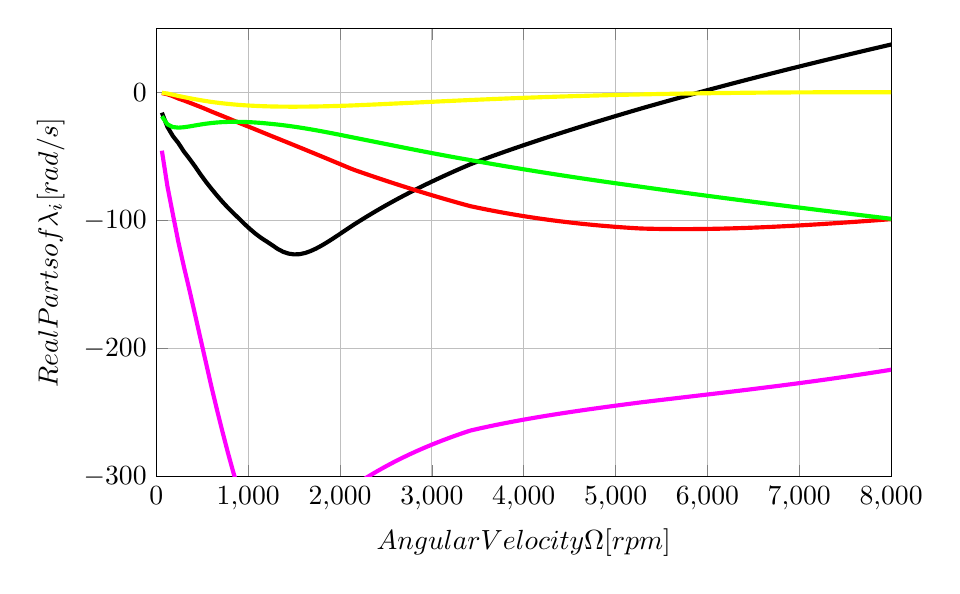
\begin{tikzpicture}

\begin{axis}[%
width=0.9\linewidth,
height=0.6\linewidth,
ymin=-300,
ymax=50,
xmin=0,
xmax=8000,
xlabel={$\text{Angular Velocity }\Omega\text{ [rpm]}$},
ylabel={$\text{Real Parts of }\lambda{}_\text{i}\text{ [rad/s]}$},
grid=major,
]
\addplot [color=black, line width=1.5pt, forget plot]
  table[row sep=crcr]{%
60	-15.9535237713727\\
120	-27.0027681574936\\
180	-34.2492085163738\\
240	-39.7123665530157\\
300	-46.325033845028\\
360	-51.910965962902\\
420	-57.7980337112896\\
480	-64.0772326163478\\
540	-69.9503097735983\\
600	-75.4033950488307\\
660	-80.6261783111265\\
720	-85.5761243717566\\
780	-90.2118086049729\\
840	-94.5222710340556\\
900	-98.5807601678979\\
960	-102.864854549932\\
1020	-106.83749967614\\
1080	-110.461677197053\\
1140	-113.693093508265\\
1200	-116.48168705662\\
1260	-119.313311891817\\
1320	-122.286622091035\\
1380	-124.537684060673\\
1440	-125.983883352464\\
1500	-126.593369206472\\
1560	-126.396765980168\\
1620	-125.480498248603\\
1680	-123.965575652555\\
1740	-121.982836056256\\
1800	-119.654183273279\\
1860	-117.082773419679\\
1920	-114.350410363874\\
1980	-111.519116989999\\
2040	-108.634452299717\\
2100	-105.729011790439\\
2160	-102.899493568159\\
2220	-100.193896055179\\
2280	-97.5373284041763\\
2340	-94.9341178943943\\
2400	-92.3863163331579\\
2460	-89.8944040589008\\
2520	-87.4577786914628\\
2580	-85.0751131397287\\
2640	-82.7445735802128\\
2700	-80.4640642412414\\
2760	-78.2312959379033\\
2820	-76.0438878250976\\
2880	-73.8994729027091\\
2940	-71.795690424006\\
3000	-69.7302450359813\\
3060	-67.7009098767948\\
3120	-65.7055686568227\\
3180	-63.7421801948693\\
3240	-61.8088217036545\\
3300	-59.9036705196311\\
3360	-58.0250021997602\\
3420	-56.1921711142472\\
3480	-54.5674170534887\\
3540	-52.9652590370951\\
3600	-51.3844389072955\\
3660	-49.8238278909201\\
3720	-48.2823249604413\\
3780	-46.7589405957094\\
3840	-45.2527411111916\\
3900	-43.762852085649\\
3960	-42.2884649927931\\
4020	-40.8288221951694\\
4080	-39.3832075400334\\
4140	-37.9509644252974\\
4200	-36.5314748093399\\
4260	-35.1241556696298\\
4320	-33.7284686876442\\
4380	-32.3439027629033\\
4440	-30.9699866656393\\
4500	-29.6062731539707\\
4560	-28.2523393688194\\
4620	-26.9078112096899\\
4680	-25.5723128833883\\
4740	-24.2454996733814\\
4800	-22.927056199921\\
4860	-21.6166748354043\\
4920	-20.3140857722783\\
4980	-19.019009864765\\
5040	-17.7312102692791\\
5100	-16.4504474577287\\
5160	-15.176509950824\\
5220	-13.9091925236439\\
5280	-12.6523667002017\\
5340	-11.4217324572681\\
5400	-10.1989006929735\\
5460	-8.98365263617866\\
5520	-7.77579228814406\\
5580	-6.57513098846104\\
5640	-5.38148596752587\\
5700	-4.1946851006421\\
5760	-3.01456288923904\\
5820	-1.84097318857587\\
5880	-0.673758677112176\\
5940	0.487214765569452\\
6000	1.64208157488331\\
6060	2.79097148181623\\
6120	3.93400326909369\\
6180	5.07128989201568\\
6240	6.20294848212495\\
6300	7.32907852714651\\
6360	8.44977503314857\\
6420	9.56514297301936\\
6480	10.675267422307\\
6540	11.7802386884117\\
6600	12.8801413749396\\
6660	13.9750536743829\\
6720	15.0650502663419\\
6780	16.1502059845077\\
6840	17.2305858752846\\
6900	18.3062594374279\\
6960	19.3772991884634\\
7020	20.443760800353\\
7080	21.505696902457\\
7140	22.5631738774703\\
7200	23.616243110374\\
7260	24.6649525551329\\
7320	25.7093584211374\\
7380	26.7495124430822\\
7440	27.785450447266\\
7500	28.8172297902397\\
7560	29.8448820292335\\
7620	30.8684501444685\\
7680	31.8879931047794\\
7740	32.9035267186508\\
7800	33.9151052519377\\
7860	34.9227520389867\\
7920	35.9265075914317\\
7980	36.9264029751755\\
8040	37.9224752249414\\
8100	-1261.36715875494\\
8160	-1253.48792246467\\
8220	-1245.89746619594\\
8280	-1238.57766460134\\
8340	-1231.46488497436\\
8400	-1224.55193841251\\
8460	-1217.83184719548\\
8520	-1211.29805046666\\
8580	-1204.94412250167\\
8640	-1198.76412614121\\
8700	-1192.75233972014\\
8760	-94.0502047682856\\
8820	-93.6283737251746\\
8880	-93.2056569289729\\
8940	-92.7822196716144\\
9000	-92.3581309097997\\
9060	-91.9335260611439\\
9120	-91.5085612980305\\
9180	-91.0832864325335\\
9240	-90.6578421036114\\
9300	-90.2323452143626\\
9360	-89.8068380655702\\
9420	-89.381465495943\\
9480	-88.9562749789174\\
9540	-88.5313600574461\\
9600	-88.1068088800141\\
9660	-87.6827243895624\\
9720	-87.2591266664398\\
9780	-86.8360755119381\\
9840	-86.4137068832956\\
9900	-85.9920237325197\\
9960	-85.5711122654958\\
10020	-85.1510334874291\\
10080	-84.7317880130719\\
10140	-84.313518256346\\
10200	-83.8961744096828\\
10260	-83.4798709832995\\
10320	-83.0646174445203\\
10380	-82.6504673171187\\
10440	-82.237447915087\\
10500	-81.8256208813137\\
10560	-81.4149660585723\\
10620	-81.0055781443491\\
10680	-80.5974331142203\\
10740	-80.1905916002321\\
10800	-79.7850848857134\\
10860	-79.3809051642762\\
10920	-78.9780911368782\\
10980	-78.5766556734642\\
11040	-78.1766449846501\\
11100	-77.7780352855438\\
11160	-77.3809082063623\\
11220	-76.9851956603114\\
11280	-76.5909622432819\\
11340	-76.1982094177683\\
11400	-75.8069678787898\\
11460	-75.4172121469165\\
11520	-75.0289732635815\\
11580	-74.6422703592467\\
11640	-74.2570634330142\\
11700	-73.8734043924682\\
11760	-73.491299527647\\
11820	-73.1107429682652\\
11880	-72.731703455293\\
11940	-72.3542659070283\\
12000	-71.9783579803642\\
12060	-71.6040400762158\\
12120	-71.2312677684274\\
12180	-70.8600520423302\\
12240	-70.4904314825799\\
12300	-70.1223458165372\\
12360	-69.7558549764643\\
12420	-69.3909148902468\\
12480	-69.0275518767641\\
12540	-68.6657517300662\\
12600	-68.3055167913149\\
12660	-67.9468655608007\\
12720	-67.5897599206112\\
12780	-67.2342187266138\\
12840	-66.8802526445262\\
12900	-66.527840850658\\
12960	-66.1769946302148\\
13020	-65.8276873754038\\
13080	-65.4799289206558\\
13140	-65.1337488995004\\
13200	-64.7891080994663\\
13260	-64.4460045087301\\
13320	-64.1044578260205\\
13380	-63.7644616590735\\
13440	-63.4259843510809\\
13500	-63.0890480503171\\
13560	-62.7536668235002\\
13620	-62.4198021213658\\
13680	-62.0819350705631\\
13740	-61.7221932826281\\
13800	-61.3646055219743\\
13860	-61.0091916795574\\
13920	-60.6559399353283\\
13980	-60.3048033247169\\
14040	-59.955795350529\\
14100	-59.6089018486589\\
14160	-59.2641081902194\\
14220	127.256434754825\\
14280	127.98506305495\\
14340	128.711236630994\\
14400	129.434988490636\\
14460	130.156340550437\\
14520	130.87530417978\\
14580	131.591889301925\\
14640	132.30611309474\\
14700	133.017975414087\\
14760	133.72752208316\\
14820	134.434735200722\\
14880	135.13965190749\\
14940	135.842264830851\\
15000	136.5426110642\\
15060	137.240697227685\\
15120	137.936525687355\\
15180	138.630126369403\\
15240	139.321507566565\\
15300	140.010684128621\\
15360	140.697670200083\\
15420	141.382472629359\\
15480	142.065121155845\\
15540	142.745617466452\\
15600	143.423980463297\\
15660	144.100224760129\\
15720	144.774359724704\\
15780	145.446405399938\\
15840	146.116376525611\\
15900	146.784285706782\\
15960	147.450133193203\\
16020	148.113954617795\\
16080	148.775750088772\\
16140	149.435531370909\\
16200	150.093326250288\\
16260	150.749139929088\\
16320	151.402979398561\\
16380	152.054866108124\\
16440	152.704813021878\\
16500	153.352832409115\\
16560	153.998942356935\\
16620	154.643144919865\\
16680	155.285453613306\\
16740	155.925884782103\\
16800	156.564454726058\\
16860	157.201191632018\\
16920	157.836079639112\\
16980	158.46914078921\\
17040	159.10038260896\\
17100	159.729838259695\\
17160	160.357496129537\\
17220	160.983385333555\\
17280	161.607511204072\\
17340	162.229877977597\\
17400	162.850507015891\\
17460	163.469420097449\\
17520	164.086603419462\\
17580	164.702082810725\\
17640	165.315875430636\\
17700	165.927981774363\\
17760	166.538421640528\\
17820	167.14720123407\\
17880	167.754317902954\\
17940	168.359819764138\\
};
\addplot [color=red, line width=1.5pt, forget plot]
  table[row sep=crcr]{%
60	-0.634785090911355\\
120	-1.57326730805758\\
180	-3.08748189819646\\
240	-4.91950256094786\\
300	-6.43597336865415\\
360	-8.09554426870448\\
420	-9.77309573755644\\
480	-11.4504872031123\\
540	-13.2118810246595\\
600	-15.0633371631906\\
660	-16.7978677410889\\
720	-18.5228316285803\\
780	-20.2832553822678\\
840	-22.0800186292708\\
900	-23.8933772733445\\
960	-25.6064893251516\\
1020	-27.3334201078566\\
1080	-29.0741025852867\\
1140	-30.8285029446625\\
1200	-32.596607189631\\
1260	-34.3524294189064\\
1320	-36.0809610564813\\
1380	-37.8158357068303\\
1440	-39.5568959818819\\
1500	-41.3040124760252\\
1560	-43.0570638527529\\
1620	-44.8159639408595\\
1680	-46.5806399812359\\
1740	-48.3510444026209\\
1800	-50.1271680410887\\
1860	-51.9089822180319\\
1920	-53.6965136179173\\
1980	-55.4897929161016\\
2040	-57.2888756902623\\
2100	-59.0938321844539\\
2160	-60.7693490896018\\
2220	-62.272112839667\\
2280	-63.7599953850233\\
2340	-65.2327471141134\\
2400	-66.6901586528128\\
2460	-68.1320095665795\\
2520	-69.5581170514282\\
2580	-70.9682983403674\\
2640	-72.3624009919562\\
2700	-73.7402762735769\\
2760	-75.1017892048769\\
2820	-76.446851254876\\
2880	-77.7753281579229\\
2940	-79.0871612805517\\
3000	-80.3822639131996\\
3060	-81.6605746061078\\
3120	-82.9220485749022\\
3180	-84.1666611025361\\
3240	-85.3943682898921\\
3300	-86.6051471883859\\
3360	-87.7989992624237\\
3420	-88.9510368409119\\
3480	-89.8627145551345\\
3540	-90.7491457650009\\
3600	-91.6104662187679\\
3660	-92.4467704470735\\
3720	-93.2582599369433\\
3780	-94.0450499650665\\
3840	-94.8073460953459\\
3900	-95.5453280046252\\
3960	-96.2591860982228\\
4020	-96.9491580570312\\
4080	-97.6154665726807\\
4140	-98.2583191095821\\
4200	-98.8780182870406\\
4260	-99.4747630653058\\
4320	-100.048876565686\\
4380	-100.600599495137\\
4440	-101.130237220298\\
4500	-101.638078803237\\
4560	-102.124435743436\\
4620	-102.589568945774\\
4680	-103.033850897312\\
4740	-103.45756687898\\
4800	-103.861055014123\\
4860	-104.244637235825\\
4920	-104.608630094925\\
4980	-104.953412570547\\
5040	-105.279286054076\\
5100	-105.586608037807\\
5160	-105.875699382668\\
5220	-106.14693366583\\
5280	-106.380181147392\\
5340	-106.500077056536\\
5400	-106.601358631952\\
5460	-106.684482988709\\
5520	-106.749880595192\\
5580	-106.798001106588\\
5640	-106.829290796915\\
5700	-106.844210017906\\
5760	-106.843160359033\\
5820	-106.82660898246\\
5880	-106.794994422245\\
5940	-106.748722566343\\
6000	-106.688255730211\\
6060	-106.613991339236\\
6120	-106.526381296813\\
6180	-106.425795208311\\
6240	-106.312706763275\\
6300	-106.187456567575\\
6360	-106.050466236557\\
6420	-105.902147335806\\
6480	-105.742836916162\\
6540	-105.572964710486\\
6600	-105.39286976469\\
6660	-105.202929303395\\
6720	-105.003494612095\\
6780	-104.794912064795\\
6840	-104.577512395051\\
6900	-104.351627845127\\
6960	-104.117620884473\\
7020	-103.875773109787\\
7080	-103.626420851518\\
7140	-103.369828279075\\
7200	-103.106315746233\\
7260	-102.836185620871\\
7320	-102.559670979758\\
7380	-102.277063381293\\
7440	-101.988648393531\\
7500	-101.694660444944\\
7560	-101.395348920187\\
7620	-101.090960638672\\
7680	-100.781735503447\\
7740	-100.467887321575\\
7800	-100.149622817628\\
7860	-99.8272040080259\\
7920	-99.5007917422034\\
7980	-99.1705928413746\\
8040	-98.836814336526\\
8100	-98.4996420774329\\
8160	-98.1592624715169\\
8220	-97.7832015219837\\
8280	-97.3760188646859\\
8340	-96.9665019835356\\
8400	-96.5548916499082\\
8460	-96.141336626641\\
8520	-95.7260233153757\\
8580	-95.3091037846938\\
8640	-94.8907127367512\\
8700	-94.4710112672367\\
8760	-1186.90310880511\\
8820	-1181.21123724474\\
8880	-1175.67164586122\\
8940	-1170.27947281526\\
9000	-1165.030033896\\
9060	-1159.91886569437\\
9120	-1154.94182552932\\
9180	-1150.09456020257\\
9240	-1145.37326298861\\
9300	-1140.77421294912\\
9360	-1136.29353957661\\
9420	-1131.92788164862\\
9480	-1127.67374066939\\
9540	-1123.52791884623\\
9600	-1119.48727238364\\
9660	-1115.54879951495\\
9720	-1111.70949453121\\
9780	-1107.96656072399\\
9840	-1104.31731125555\\
9900	-1100.75914810815\\
9960	-1097.28942084196\\
10020	-1093.90583535872\\
10080	-1090.6058623018\\
10140	-1087.38733183481\\
10200	-1084.24798022005\\
10260	-1081.18570182185\\
10320	-1078.19845989835\\
10380	-1075.28411542502\\
10440	-1072.44085433469\\
10500	-1069.66676468005\\
10560	-1066.96004520547\\
10620	-1064.31895871056\\
10680	-1061.741703666\\
10740	-1059.22675773177\\
10800	-1056.77242536066\\
10860	-1054.37719863979\\
10920	-1052.03952119278\\
10980	-1049.75796137122\\
11040	-1047.53121003211\\
11100	-1045.35772734147\\
11160	-1043.23625820913\\
11220	-1041.16547533001\\
11280	-1039.14421238573\\
11340	-1037.17114770824\\
11400	-1035.24516676552\\
11460	-1033.36505652689\\
11520	-1031.52974132865\\
11580	-1029.73813661019\\
11640	-1027.98916477907\\
11700	-1026.28182446768\\
11760	-1024.61513636336\\
11820	-1022.98807325761\\
11880	-1021.39971910296\\
11940	-1019.84914581126\\
12000	-1018.33550232624\\
12060	-1016.85789956848\\
12120	-1015.41551555076\\
12180	-1014.00747193912\\
12240	-1012.63304795744\\
12300	-1011.29138902244\\
12360	-1009.98181362922\\
12420	-1008.70352584974\\
12480	-1007.4558430651\\
12540	-1006.23808685602\\
12600	-1005.04949901509\\
12660	-1003.88949636898\\
12720	-1002.75741073159\\
12780	-1001.65258693014\\
12840	-1000.57444802734\\
12900	-999.522396103008\\
12960	-998.495853144231\\
13020	-997.494210564215\\
13080	-996.516991561631\\
13140	-995.563567665232\\
13200	-994.6335035158\\
13260	-993.726256422917\\
13320	-992.841323618357\\
13380	-991.978204855515\\
13440	-991.136434957127\\
13500	-990.315585643653\\
13560	-989.515144962166\\
13620	-988.734719075192\\
13680	-988.073754032915\\
13740	-987.858117461614\\
13800	-987.654392853969\\
13860	-987.462295628886\\
13920	-987.281701659466\\
13980	-987.112231752798\\
14040	-986.953704565176\\
14100	-986.80580884116\\
14160	-986.668324093985\\
14220	-986.541112316595\\
14280	-986.423881496551\\
14340	-986.316299543001\\
14400	-986.218302805644\\
14460	-986.12965500625\\
14520	-986.050078903935\\
14580	-985.979457477221\\
14640	-985.917540705369\\
14700	-985.864145282946\\
14760	-985.819120322445\\
14820	-985.782248060232\\
14880	-985.753335902932\\
14940	-985.732198886101\\
15000	-985.718737861592\\
15060	-985.712748862806\\
15120	-985.71403595217\\
15180	-985.7224707794\\
15240	-985.737914923463\\
15300	-985.760204418205\\
15360	-985.789138931388\\
15420	-985.824612878662\\
15480	-985.866523254247\\
15540	-985.914667530708\\
15600	-985.968959627177\\
15660	-986.029218989058\\
15720	-986.095346817953\\
15780	-986.167239369903\\
15840	-986.244720175687\\
15900	-986.327705728044\\
15960	-986.416006984375\\
16020	-986.509610979569\\
16080	-986.608333934536\\
16140	-986.712090795297\\
16200	-986.820783287959\\
16260	-986.934294355021\\
16320	-987.052494472707\\
16380	-987.175315334447\\
16440	-987.302657247227\\
16500	-987.434395126628\\
16560	-987.570454670423\\
16620	-987.71073266512\\
16680	-987.855134289868\\
16740	-988.003611147076\\
16800	-988.155986589899\\
16860	-988.312300870783\\
16920	-988.472354815573\\
16980	-988.636155457722\\
17040	-988.803522408073\\
17100	-988.97445948375\\
17160	-989.148903908012\\
17220	-989.326692223214\\
17280	-989.507855172749\\
17340	-989.692216339372\\
17400	-989.879775457808\\
17460	-990.07043936337\\
17520	-990.264108758416\\
17580	-990.460816502857\\
17640	-990.660420146293\\
17700	-990.862836449316\\
17760	-991.068056931018\\
17820	-991.276036222971\\
17880	-991.48660187197\\
17940	-991.699885789654\\
};
\addplot [color=mycolor1, line width=1.5pt, forget plot]
  table[row sep=crcr]{%
60	-45.6324568226401\\
120	-73.3489573695338\\
180	-95.4338768216743\\
240	-117.167337052117\\
300	-136.296262467286\\
360	-154.431752396742\\
420	-173.206271348184\\
480	-192.260359781744\\
540	-211.147234327967\\
600	-230.0553890955\\
660	-247.910916878157\\
720	-265.115853988378\\
780	-281.694551912313\\
840	-297.29156642312\\
900	-311.438185653451\\
960	-323.625721886836\\
1020	-333.369211629031\\
1080	-340.587886428014\\
1140	-345.451403979025\\
1200	-348.287606816285\\
1260	-349.635098510583\\
1320	-349.615145698018\\
1380	-348.341118155159\\
1440	-346.199598862493\\
1500	-343.476066277872\\
1560	-340.375717021965\\
1620	-337.044787798649\\
1680	-333.58588545892\\
1740	-330.071308069747\\
1800	-326.551459568982\\
1860	-323.060890753444\\
1920	-319.623252263515\\
1980	-316.254412556233\\
2040	-312.964366382725\\
2100	-309.759131392857\\
2160	-306.733266247646\\
2220	-303.914303269521\\
2280	-301.193245650472\\
2340	-298.567744788354\\
2400	-296.03495352327\\
2460	-293.591648582699\\
2520	-291.234639850514\\
2580	-288.960358927791\\
2640	-286.76558883017\\
2700	-284.646842428258\\
2760	-282.600795516629\\
2820	-280.624359606553\\
2880	-278.714275289653\\
2940	-276.867590446916\\
3000	-275.081348115147\\
3060	-273.352937526154\\
3120	-271.679434778563\\
3180	-270.058480638208\\
3240	-268.487579674604\\
3300	-266.964289076413\\
3360	-265.486443961507\\
3420	-264.093372687442\\
3480	-263.100814442469\\
3540	-262.137486503783\\
3600	-261.202277257923\\
3660	-260.293484848073\\
3720	-259.410091247493\\
3780	-258.550866310358\\
3840	-257.714527836515\\
3900	-256.900041782918\\
3960	-256.106239110599\\
4020	-255.332066295079\\
4080	-254.576573428455\\
4140	-253.838818322282\\
4200	-253.117695603335\\
4260	-252.412417054013\\
4320	-251.721958023805\\
4380	-251.045593180548\\
4440	-250.382349333633\\
4500	-249.73155013693\\
4560	-249.092385583691\\
4620	-248.463896496999\\
4680	-247.845454436055\\
4740	-247.236373685765\\
4800	-246.635866545777\\
4860	-246.043287585429\\
4920	-245.457831483285\\
4980	-244.878984179077\\
5040	-244.305988528903\\
5100	-243.7383237917\\
5160	-243.175333411763\\
5220	-242.616337804677\\
5280	-242.066379954191\\
5340	-241.545867707236\\
5400	-241.029215422153\\
5460	-240.515937991838\\
5520	-240.005512706413\\
5580	-239.497428559695\\
5640	-238.991069827156\\
5700	-238.48603045246\\
5760	-237.981986091536\\
5820	-237.478147767747\\
5880	-236.97439690366\\
5940	-236.470069225921\\
6000	-235.964843624385\\
6060	-235.458345131042\\
6120	-234.950090088158\\
6180	-234.43980415877\\
6240	-233.927022683312\\
6300	-233.411547565381\\
6360	-232.892856363148\\
6420	-232.370755122707\\
6480	-231.845001874357\\
6540	-231.315088481424\\
6600	-230.780942468286\\
6660	-230.242165081117\\
6720	-229.698683094137\\
6780	-229.150158872522\\
6840	-228.596198914002\\
6900	-228.036750837646\\
6960	-227.471673174598\\
7020	-226.900807503786\\
7080	-226.323675158443\\
7140	-225.740542352593\\
7200	-225.151019293818\\
7260	-224.554873409831\\
7320	-223.952286280271\\
7380	-223.343010764657\\
7440	-222.726892451108\\
7500	-222.103946342936\\
7560	-221.474061957115\\
7620	-220.836973504447\\
7680	-220.193094472313\\
7740	-219.541951395479\\
7800	-218.883902553934\\
7860	-218.218582951404\\
7920	-217.546061358144\\
7980	-216.866516836007\\
8040	-216.179858416883\\
8100	-215.486121205316\\
8160	-214.785322288302\\
8220	-213.995683748394\\
8280	-213.129235428757\\
8340	-212.258024126909\\
8400	-211.382052193355\\
8460	-210.501270229596\\
8520	-209.615878639668\\
8580	-208.725760195651\\
8640	-207.831082863106\\
8700	-206.932100843916\\
8760	-206.028455041009\\
8820	-205.12050129441\\
8880	-204.208355046715\\
8940	-203.29191525366\\
9000	-202.371313221128\\
9060	-201.446766613338\\
9120	-200.51842724082\\
9180	-199.586062338327\\
9240	-198.650038103946\\
9300	-197.710612341283\\
9360	-196.767511717886\\
9420	-195.821075439924\\
9480	-194.871320681152\\
9540	-193.918456644922\\
9600	-192.962488810575\\
9660	-192.003768790261\\
9720	-191.042155148639\\
9780	-190.07790659548\\
9840	-189.111022856306\\
9900	-188.141852220433\\
9960	-187.170200754258\\
10020	-186.196467130709\\
10080	-185.22060612026\\
10140	-184.242682323722\\
10200	-183.263057706545\\
10260	-182.281681506637\\
10320	-181.298877423837\\
10380	-180.314342420888\\
10440	-179.328563571376\\
10500	-178.341433975228\\
10560	-177.353418782996\\
10620	-176.364338462709\\
10680	-175.374209177707\\
10740	-174.383464216882\\
10800	-173.391999879709\\
10860	-172.399997901177\\
10920	-171.407439144703\\
10980	-170.414428047992\\
11040	-169.421500109223\\
11100	-168.428239762314\\
11160	-167.434817545912\\
11220	-166.441537961572\\
11280	-165.448511885123\\
11340	-164.455629988484\\
11400	-163.463052977074\\
11460	-162.470961559542\\
11520	-161.479309595844\\
11580	-160.488310510132\\
11640	-159.497987485723\\
11700	-158.508438548705\\
11760	-157.519767480535\\
11820	-156.531943838247\\
11880	-155.545302348806\\
11940	-154.559407775473\\
12000	-153.57496101594\\
12060	-152.591480811311\\
12120	-151.609401317232\\
12180	-150.628652186536\\
12240	-149.64944916446\\
12300	-148.671662455109\\
12360	-147.695433044709\\
12420	-146.720758495014\\
12480	-145.747809987335\\
12540	-144.776672929886\\
12600	-143.8072040398\\
12660	-142.839476677363\\
12720	-141.873747580583\\
12780	-140.909880780276\\
12840	-139.947970299418\\
12900	-138.988157949907\\
12960	-138.030339418318\\
13020	-137.074666129034\\
13080	-136.121317118847\\
13140	-135.169871050711\\
13200	-134.220775710492\\
13260	-133.274018057192\\
13320	-132.329608646618\\
13380	-131.387371132203\\
13440	-130.447568293406\\
13500	-129.510320260802\\
13560	-128.575287321594\\
13620	-127.642769055213\\
13680	-126.722522246657\\
13740	-125.84716980333\\
13800	-124.973877825889\\
13860	-124.102628592066\\
13920	-123.233681110761\\
13980	-122.367008315827\\
14040	-121.502585725744\\
14100	-120.64034191193\\
14160	-119.780256760454\\
14220	-118.922548525934\\
14280	-118.067363872044\\
14340	-117.214078821899\\
14400	-116.363260728151\\
14460	-115.51482045684\\
14520	-114.668647525233\\
14580	-113.824979160825\\
14640	-112.983606340139\\
14700	-112.144503586869\\
14760	-111.308054395071\\
14820	-110.473753856205\\
14880	-109.641946464568\\
14940	-108.812449289043\\
15000	-107.985448384573\\
15060	-107.160968155296\\
15120	-106.338647331321\\
15180	-105.519012033734\\
15240	-104.701752022836\\
15300	-103.886908808907\\
15360	-103.074495262136\\
15420	-102.264497368614\\
15480	-101.4569956974\\
15540	-100.651982100138\\
15600	-99.84943287467\\
15660	-99.0492398392583\\
15720	-98.2516131226304\\
15780	-97.4564434840798\\
15840	-96.6636484303502\\
15900	-95.8734953748746\\
15960	-95.0854638701662\\
16020	-94.3002171330113\\
16080	-93.5172319760896\\
16140	-92.7367262442775\\
16200	-91.9588267261693\\
16260	-91.1833692372834\\
16320	-90.410180505134\\
16380	-89.6395349121906\\
16440	-88.8714530764008\\
16500	-88.105688880397\\
16560	-87.3425410807162\\
16620	-86.5816259105218\\
16680	-85.8232221003054\\
16740	-85.0672331738187\\
16800	-84.3136303663191\\
16860	-83.562637159832\\
16920	-82.8138590764077\\
16980	-82.0676419508945\\
17040	-81.3237154682285\\
17100	-80.5821769572118\\
17160	-79.8431384760048\\
17220	-79.106523362792\\
17280	-78.3723132824318\\
17340	-77.6403890895142\\
17400	-76.9108914647116\\
17460	-76.1838321122413\\
17520	-75.4588724462115\\
17580	-74.7365685606369\\
17640	-74.0166290127713\\
17700	-73.2988276875791\\
17760	-72.5835100046577\\
17820	-71.870596116562\\
17880	-71.1596972852874\\
17940	-70.4515752622843\\
};
\addplot [color=mycolor2, line width=1.5pt, forget plot]
  table[row sep=crcr]{%
60	-0.407376310136437\\
120	-1.0084815909232\\
180	-1.90072812961505\\
240	-2.91716696607875\\
300	-3.76209722964898\\
360	-4.62410622719283\\
420	-5.42858677457318\\
480	-6.1674222157221\\
540	-6.87479674680998\\
600	-7.54815363364689\\
660	-8.11734525076324\\
720	-8.62452808849658\\
780	-9.08610184774486\\
840	-9.50450826313933\\
900	-9.87414158985293\\
960	-10.1696609656193\\
1020	-10.426095315327\\
1080	-10.6457758167546\\
1140	-10.8309771255214\\
1200	-10.9826938182836\\
1260	-11.0985834726682\\
1320	-11.1770853399826\\
1380	-11.2304547868942\\
1440	-11.2599570838652\\
1500	-11.2666798761882\\
1560	-11.2520639831595\\
1620	-11.2183158952918\\
1680	-11.1660020253001\\
1740	-11.0969084640175\\
1800	-11.0110499751236\\
1860	-10.9108713738523\\
1920	-10.7971826757685\\
1980	-10.6708177973799\\
2040	-10.5328726908637\\
2100	-10.3843630035882\\
2160	-10.2201486957775\\
2220	-10.0407975416382\\
2280	-9.85601215533241\\
2340	-9.66662241707355\\
2400	-9.47335045304488\\
2460	-9.27644377386653\\
2520	-9.07696040351799\\
2580	-8.87496264938015\\
2640	-8.67161946041799\\
2700	-8.46714341484238\\
2760	-8.26212133695056\\
2820	-8.05642234876554\\
2880	-7.85103813999851\\
2940	-7.64584436765336\\
3000	-7.44180267780888\\
3060	-7.23860833653723\\
3120	-7.03666227672968\\
3180	-6.83575562241921\\
3240	-6.63724139163648\\
3300	-6.4404970496127\\
3360	-6.24576770232066\\
3420	-6.05367561591546\\
3480	-5.86544797073\\
3540	-5.68008652834234\\
3600	-5.49801656068624\\
3660	-5.31848332476798\\
3720	-5.14201771018846\\
3780	-4.96865200034941\\
3840	-4.79823963184295\\
3900	-4.63101614704335\\
3960	-4.46696480668847\\
4020	-4.30587461691966\\
4080	-4.14806120407249\\
4140	-3.99397573533998\\
4200	-3.84237729941676\\
4260	-3.69478475120384\\
4320	-3.54965761923636\\
4380	-3.40827460053272\\
4440	-3.26982639871554\\
4500	-3.13473679997655\\
4560	-3.00304384913245\\
4620	-2.87456778846223\\
4680	-2.74894215910181\\
4740	-2.62677594888528\\
4800	-2.50771933180011\\
4860	-2.39187594399616\\
4920	-2.27890459082023\\
4980	-2.16923180166359\\
5040	-2.06249173853908\\
5100	-1.95892188307746\\
5160	-1.85852736299745\\
5220	-1.76086943535289\\
5280	-1.66637576661065\\
5340	-1.57523437850656\\
5400	-1.48687895289068\\
5460	-1.40147990710992\\
5520	-1.31902155335971\\
5580	-1.23923527312094\\
5640	-1.16218034704828\\
5700	-1.08771047723693\\
5760	-1.01644016608537\\
5820	-0.947389983784932\\
5880	-0.881240348020291\\
5940	-0.817786910927916\\
6000	-0.756730960535924\\
6060	-0.698512996457879\\
6120	-0.642600010649758\\
6180	-0.589458983440084\\
6240	-0.53849643989325\\
6300	-0.490326561422321\\
6360	-0.444351059679594\\
6420	-0.400818003895415\\
6480	-0.359933553096561\\
6540	-0.321135160994824\\
6600	-0.284761917865478\\
6660	-0.250616544529938\\
6720	-0.21898830702706\\
6780	-0.189581824074657\\
6840	-0.162265509129779\\
6900	-0.137180549677978\\
6960	-0.1142811242988\\
7020	-0.0937924579973175\\
7080	-0.0749637350010927\\
7140	-0.0586391021101592\\
7200	-0.0443260987758837\\
7260	-0.0316148115518095\\
7320	-0.0214510922718456\\
7380	-0.0133488446615328\\
7440	-0.00703314065479265\\
7500	-0.00283885572918291\\
7560	-0.000569666492813203\\
7620	0.000137646622668015\\
7680	-0.00155781796531879\\
7740	-0.00474888489372149\\
7800	-0.0103643750074445\\
7860	-0.01740000026746\\
7920	-0.0261897633921287\\
7980	-0.0370106706797935\\
8040	-0.0495546146573384\\
8100	-0.0639453883525876\\
8160	-0.0799946556325671\\
8220	-0.0976470571530619\\
8280	-0.117083820567583\\
8340	-0.138390525116664\\
8400	-0.161268607011383\\
8460	-0.185687015797745\\
8520	-0.211879355720159\\
8580	-0.239548711353711\\
8640	-0.268931795523542\\
8700	-0.300086233593296\\
8760	-0.33254906878947\\
8820	-0.36655755175365\\
8880	-0.402316474990016\\
8940	-0.439327004313486\\
9000	-0.477899193370683\\
9060	-0.518025016818358\\
9120	-0.559775717961757\\
9180	-0.60274009416472\\
9240	-0.647216792515379\\
9300	-0.693242860965508\\
9360	-0.74055881625236\\
9420	-0.78928276228362\\
9480	-0.839393142478781\\
9540	-0.890886353767685\\
9600	-0.943669979627727\\
9660	-0.997956986475855\\
9720	-1.05342976941241\\
9780	-1.11040900389464\\
9840	-1.16849970539434\\
9900	-1.22805270069564\\
9960	-1.28867146093238\\
10020	-1.35067010804224\\
10080	-1.41399060175507\\
10140	-1.47823022118408\\
10200	-1.54397622030477\\
10260	-1.61084963916702\\
10320	-1.67909352047543\\
10380	-1.7482611828195\\
10440	-1.81876506632723\\
10500	-1.8902116129946\\
10560	-1.9631870964325\\
10620	-2.03714735847203\\
10680	-2.11218145733808\\
10740	-2.18842057294258\\
10800	-2.26575782507685\\
10860	-2.34421524513927\\
10920	-2.42371044870085\\
10980	-2.50416005595837\\
11040	-2.58600238685367\\
11100	-2.66874795743244\\
11160	-2.75233209060776\\
11220	-2.83716078176088\\
11280	-2.92312016704723\\
11340	-3.00994410966857\\
11400	-3.09774837674291\\
11460	-3.18669598608918\\
11520	-3.27646086928921\\
11580	-3.36731351937684\\
11640	-3.45917026461331\\
11700	-3.55197962665672\\
11760	-3.64572716591944\\
11820	-3.74040009668616\\
11880	-3.83619789994203\\
11940	-3.93255637117476\\
12000	-4.03018362998068\\
12060	-4.12837562663608\\
12120	-4.22762243726041\\
12180	-4.32778578112131\\
12240	-4.42887883210685\\
12300	-4.53088080788497\\
12360	-4.63366747260915\\
12420	-4.73730421140927\\
12480	-4.84187561160836\\
12540	-4.94735650148582\\
12600	-5.0536180895116\\
12660	-5.16054140718393\\
12720	-5.26847654948119\\
12780	-5.37712393077492\\
12840	-5.48657411956424\\
12900	-5.59688651799509\\
12960	-5.70789677384588\\
13020	-5.8197849681045\\
13080	-5.93260273095839\\
13140	-6.04587383375581\\
13200	-6.16002791125269\\
13260	-6.27506823910002\\
13320	-6.39087549898685\\
13380	-6.50722807573106\\
13440	-6.62439355535677\\
13500	-6.74247926372448\\
13560	-6.86099041616866\\
13620	-6.98032730152553\\
13680	-7.10060965357612\\
13740	-7.22294473121768\\
13800	-7.34597550668945\\
13860	-7.46960280524095\\
13920	-7.59403252418726\\
13980	-7.71929606348079\\
14040	-7.84524316303424\\
14100	-7.97188144852224\\
14160	-8.09910695938213\\
14220	-8.22710306537701\\
14280	-8.35602477287968\\
14340	-8.48528925319171\\
14400	-8.6153318647002\\
14460	-8.74609964447441\\
14520	-8.87747983219224\\
14580	-9.00965775166321\\
14640	-9.14243737995251\\
14700	-9.27577007598466\\
14760	-9.41004313462303\\
14820	-9.54465981519638\\
14880	-9.68003111819762\\
14940	-9.81596354560355\\
15000	-9.95256559015893\\
15060	-10.0899080706512\\
15120	-10.22761645289\\
15180	-10.3661602056451\\
15240	-10.5052761763926\\
15300	-10.6449375342525\\
15360	-10.785209264228\\
15420	-10.9260484778878\\
15480	-11.0675091462633\\
15540	-11.2095931080509\\
15600	-11.3522414845802\\
15660	-11.4953821176333\\
15720	-11.6391945308791\\
15780	-11.7835834275929\\
15840	-11.9284096992284\\
15900	-12.0739832579155\\
15960	-12.2198061154767\\
16020	-12.3664675049851\\
16080	-12.5134994409081\\
16140	-12.6610554365158\\
16200	-12.8093028672444\\
16260	-12.9580784505777\\
16320	-13.1071751342604\\
16380	-13.2568939076866\\
16440	-13.4072372620156\\
16500	-13.5579579071081\\
16560	-13.7093778322341\\
16620	-13.8610785547597\\
16680	-14.0133642025546\\
16740	-14.1661196409373\\
16800	-14.3193638656737\\
16860	-14.473201403144\\
16920	-14.6273665744536\\
16980	-14.7821378575283\\
17040	-14.9372964610267\\
17100	-15.0928725823353\\
17160	-15.2490079378948\\
17220	-15.4056733461482\\
17280	-15.5627826870996\\
17340	-15.7202518798386\\
17400	-15.8782434531182\\
17460	-16.036728468355\\
17520	-16.1954059696251\\
17580	-16.3548197648863\\
17640	-16.5146512768445\\
17700	-16.6747448780911\\
17760	-16.8354007845646\\
17820	-16.9965308658928\\
17880	-17.1578232458316\\
17940	-17.3198953312503\\
};
\addplot [color=green, line width=1.5pt, forget plot]
  table[row sep=crcr]{%
60	-18.7904124394339\\
120	-25.0238492890537\\
180	-27.1474122437005\\
240	-27.6316672477321\\
300	-27.302359697662\\
360	-26.6780576308732\\
420	-25.936636304512\\
480	-25.1999643255325\\
540	-24.5478990499881\\
600	-24.0062116017952\\
660	-23.5990379765995\\
720	-23.3129995551093\\
780	-23.1385674914165\\
840	-23.0674961916615\\
900	-23.0916045453415\\
960	-23.188463123352\\
1020	-23.3681645886601\\
1080	-23.6237642530924\\
1140	-23.9487657464753\\
1200	-24.3384678062253\\
1260	-24.7620818362314\\
1320	-25.2137837165355\\
1380	-25.720795131122\\
1440	-26.2789595250998\\
1500	-26.884491691246\\
1560	-27.533311067822\\
1620	-28.2204386969794\\
1680	-28.9431054453346\\
1740	-29.6969694614163\\
1800	-30.4800447648286\\
1860	-31.2873001152349\\
1920	-32.1158491260874\\
1980	-32.9627451515489\\
2040	-33.8247614777458\\
2100	-34.6988206163376\\
2160	-35.5632575350388\\
2220	-36.4135393643902\\
2280	-37.2696241552624\\
2340	-38.1297680249141\\
2400	-38.9923630893278\\
2460	-39.8565716775525\\
2520	-40.7203073263241\\
2580	-41.5830940092822\\
2640	-42.4427786933237\\
2700	-43.2986867672134\\
2760	-44.1495715474761\\
2820	-44.9951970193488\\
2880	-45.8339390517172\\
2940	-46.6655666793863\\
3000	-47.4885032686085\\
3060	-48.3028968980809\\
3120	-49.10799213291\\
3180	-49.9038685901672\\
3240	-50.6884298401513\\
3300	-51.462495790597\\
3360	-52.225551273214\\
3420	-52.9799351208504\\
3480	-53.7522417369923\\
3540	-54.5172907697506\\
3600	-55.2744464731229\\
3660	-56.0250358399693\\
3720	-56.7682896101988\\
3780	-57.5042460004603\\
3840	-58.2332839902967\\
3900	-58.955051542727\\
3960	-59.6698287532428\\
4020	-60.3779252442034\\
4080	-61.0789887311897\\
4140	-61.7724450701074\\
4200	-62.4603085769111\\
4260	-63.140379551508\\
4320	-63.8151303557804\\
4380	-64.482624416686\\
4440	-65.1443590284899\\
4500	-65.7996143947292\\
4560	-66.4485685658203\\
4620	-67.0915666487359\\
4680	-67.7292721858952\\
4740	-68.3608654244651\\
4800	-68.9869339301409\\
4860	-69.6074883095777\\
4920	-70.2231315204906\\
4980	-70.8332646271454\\
5040	-71.4385706418357\\
5100	-72.0387644738158\\
5160	-72.6338794661379\\
5220	-73.2248226669878\\
5280	-73.8148056494739\\
5340	-74.4184854255278\\
5400	-75.0188832128815\\
5460	-75.6157785221967\\
5520	-76.2092401165769\\
5580	-76.7997939059618\\
5640	-77.3873187675813\\
5700	-77.9722067323457\\
5760	-78.553258348458\\
5820	-79.1323525450369\\
5880	-79.7082878457068\\
5940	-80.2814921650128\\
6000	-80.8524096291725\\
6060	-81.4203263574393\\
6120	-81.9863085390938\\
6180	-82.5494457470511\\
6240	-83.1108383433221\\
6300	-83.6693912536976\\
6360	-84.2262249745853\\
6420	-84.7809207921351\\
6480	-85.3330351845323\\
6540	-85.8836419737112\\
6600	-86.4321227899854\\
6660	-86.9789519961996\\
6720	-87.5234605980486\\
6780	-88.066242404321\\
6840	-88.6075620981433\\
6900	-89.1471971739765\\
6960	-89.6851879245525\\
7020	-90.2210992315914\\
7080	-90.7563929293712\\
7140	-91.2894212323798\\
7200	-91.821129090325\\
7260	-92.3523711609807\\
7320	-92.8811951513736\\
7380	-93.4086483217008\\
7440	-93.9352286341729\\
7500	-94.4602261169069\\
7560	-94.984040435624\\
7620	-95.5074764818644\\
7680	-96.0287360819528\\
7740	-96.5496687497376\\
7800	-97.0683311377804\\
7860	-97.5867866664054\\
7920	-98.1044648440386\\
7980	-98.6206170020082\\
8040	-99.1358968240235\\
8100	-99.6501281042638\\
8160	-100.163607602982\\
8220	-100.667140869516\\
8280	-101.161322937127\\
8340	-101.65410852499\\
8400	-102.146056979317\\
8460	-102.637286162052\\
8520	-103.127279269179\\
8580	-103.616513826547\\
8640	-104.104671798091\\
8700	-104.59142314545\\
8760	-105.077838012612\\
8820	-105.563421941689\\
8880	-106.047620383306\\
8940	-106.531595987643\\
9000	-107.014520145163\\
9060	-107.496514757858\\
9120	-107.977406387186\\
9180	-108.457916921243\\
9240	-108.937588943729\\
9300	-109.416210910419\\
9360	-109.894309841231\\
9420	-110.371691980423\\
9480	-110.8482688413\\
9540	-111.324197811302\\
9600	-111.799495881204\\
9660	-112.273753480436\\
9720	-112.747724289486\\
9780	-113.220461301624\\
9840	-113.693013371292\\
9900	-114.164603472699\\
9960	-114.636020216283\\
10020	-115.106485232157\\
10080	-115.57622900273\\
10140	-116.046128456637\\
10200	-116.514734820348\\
10260	-116.983036764769\\
10320	-117.45029191437\\
10380	-117.917671299293\\
10440	-118.384113743426\\
10500	-118.850580455617\\
10560	-119.315616821212\\
10620	-119.780529844966\\
10680	-120.245034629849\\
10740	-120.708828382083\\
10800	-121.172240010095\\
10860	-121.635133671022\\
10920	-122.097655554397\\
10980	-122.559981217553\\
11040	-123.021029749444\\
11100	-123.482142546346\\
11160	-123.943334869486\\
11220	-124.403556785311\\
11280	-124.863071463722\\
11340	-125.322618624804\\
11400	-125.78193808542\\
11460	-126.240333209442\\
11520	-126.698906416792\\
11580	-127.156798387555\\
11640	-127.614265899479\\
11700	-128.071401759304\\
11760	-128.528255698425\\
11820	-128.984863227473\\
11880	-129.440634085505\\
11940	-129.897019475446\\
12000	-130.352168005817\\
12060	-130.808032045496\\
12120	-131.263093481048\\
12180	-131.717799818814\\
12240	-132.172229796073\\
12300	-132.626289319311\\
12360	-133.080398701232\\
12420	-133.534175683532\\
12480	-133.987457669306\\
12540	-134.440459960369\\
12600	-134.893383142169\\
12660	-135.34650220243\\
12720	-135.798898079712\\
12780	-136.251509496316\\
12840	-136.703949551832\\
12900	-137.155927923667\\
12960	-137.608020383772\\
13020	-138.059723654245\\
13080	-138.511011604225\\
13140	-138.962860638595\\
13200	-139.414414087415\\
13260	-139.865358013643\\
13320	-140.316226222745\\
13380	-140.767516657334\\
13440	-141.218596451283\\
13500	-141.668936774968\\
13560	-142.120237138915\\
13620	-142.571034254789\\
13680	-143.034350434928\\
13740	-143.550576991752\\
13800	-144.067105322475\\
13860	-144.584245660614\\
13920	-145.101281517182\\
13980	-145.618252059949\\
14040	-146.135442549717\\
14100	-146.652817488143\\
14160	-147.170940169487\\
14220	-147.688974357155\\
14280	-148.20654945668\\
14340	-148.725270523175\\
14400	-149.244015754678\\
14460	-149.762878238928\\
14520	-150.28213794801\\
14580	-150.801227785136\\
14640	-151.320841912173\\
14700	-151.840909475624\\
14760	-152.36031396641\\
14820	-152.881204351851\\
14880	-153.401765036602\\
14940	-153.922924298774\\
15000	-154.444376744652\\
15060	-154.965754657366\\
15120	-155.488223499641\\
15180	-156.010228650674\\
15240	-156.532775704748\\
15300	-157.05574173356\\
15360	-157.579262813785\\
15420	-158.103046182774\\
15480	-158.627243921787\\
15540	-159.151620485212\\
15600	-159.676513160978\\
15660	-160.202085058832\\
15720	-160.727748561372\\
15780	-161.253556075434\\
15840	-161.780514498547\\
15900	-162.307126666863\\
15960	-162.835344908421\\
16020	-163.362887608716\\
16080	-163.891627747083\\
16140	-164.421069551645\\
16200	-164.950334849024\\
16260	-165.479908400317\\
16320	-166.011137588875\\
16380	-166.542338485261\\
16440	-167.07375310491\\
16500	-167.606047985271\\
16560	-168.138578409016\\
16620	-168.672373521899\\
16680	-169.206532489471\\
16740	-169.741290896464\\
16800	-170.276736490949\\
16860	-170.812560199899\\
16920	-171.34954777464\\
16980	-171.886912771517\\
17040	-172.425241921123\\
17100	-172.96452094007\\
17160	-173.504167214661\\
17220	-174.044499211375\\
17280	-174.585613278793\\
17340	-175.127863576525\\
17400	-175.670783865957\\
17460	-176.214348968964\\
17520	-176.759895462281\\
17580	-177.30516446508\\
17640	-177.851431143777\\
17700	-178.399454325152\\
17760	-178.947972311825\\
17820	-179.497253228474\\
17880	-180.048723050509\\
17940	-180.599748536278\\
};
\addplot[black, dashed, samples=2] {0};
\end{axis}

\end{tikzpicture}%
    \caption{Stability map of Hydrodynamic Bearing}
    \label{fig:hydrodynamic_bearing_stability_map}
\end{figure}
The maximum angular velocity is now approximatly 6000 rpm. This is a increase from 5500 rpm of approximatly $9 \%$.